% Layout revision: simple continuous tabulars, one data row per block.
% Complete typed-quantifier and predicate-hyperlink revision, 2026-11-20.
% Source: uploads/Modular_Mills_typed_quantifiers.tex; link idiom: uploads/FTC.tex
% Original preserved. Retains the ten classical and ten finite route orders.
% Mathematical Lean-style contracts, not a compiled Lean formalization.
% TeX and Lean compilers unavailable: static checks only.
\documentclass[11pt,reqno]{amsart}
\usepackage{mathtools,adjustbox}
\usepackage{amsfonts}
\usepackage[utf8]{inputenc}
\usepackage{amsmath,amssymb,amsthm}
\usepackage{changepage}
\usepackage{ragged2e}
\usepackage{float}
\usepackage{array}
\usepackage{graphicx}
\usepackage{setspace}
\usepackage{xcolor}
\usepackage{enumitem}
\usepackage[margin=17mm]{geometry}
\setlength{\tabcolsep}{3pt}
\renewcommand{\arraystretch}{1.35}
\renewcommand{\tablename}{$\textsf{Tab}$}
\setlength{\tabcolsep}{3pt}
\renewcommand{\arraystretch}{1.2}
% Tables use simple paragraph columns and one data row per block.
\setcounter{MaxMatrixCols}{20}
\newcommand{\N}{\mathbb N}
\newcommand{\Z}{\mathbb Z}
\newcommand{\Q}{\mathbb Q}
\newcommand{\R}{\mathbb R}
\newcommand{\C}{\mathbb C}
\newcommand{\Np}{\N_{\ge1}}
\newcommand{\fl}[1]{\left\lfloor #1\right\rfloor}

\usepackage{tikz}
\usetikzlibrary{arrows.meta,positioning}
\usepackage{fancyvrb}
\usepackage{fancyhdr}
\usepackage{titlesec,titletoc}
\usepackage[colorlinks=true,linkcolor=blue,citecolor=green,urlcolor=magenta]{hyperref}
\usepackage{aliascnt}
\usepackage[nameinlink]{cleveref}
\usepackage{listings}
\usepackage{booktabs}
\providecommand{\TEXTsymbol}[1]{#1}
% Nonfloating table captions; each simple tabular contains one data row.
\makeatletter
\newcommand{\SplitTableCaption}{\def\@captype{table}\caption}
\makeatother
\restylefloat{figure}
\hypersetup{pageanchor=false}
\makeatletter
\@ifundefined{theorem}{}{\let\theorem\relax}
\@ifundefined{definition}{}{\let\definition\relax}
\@ifundefined{lemma}{}{\let\lemma\relax}
\@ifundefined{corollary}{}{\let\corollary\relax}
\@ifundefined{proposition}{}{\let\proposition\relax}
\@ifundefined{remark}{}{\let\remark\relax}
\@ifundefined{statement}{}{\let\statement\relax}
\makeatother
\DeclareUnicodeCharacter{03B9}{\ensuremath{\iota}}
\DeclareUnicodeCharacter{2200}{\ensuremath{\forall}}
\DeclareUnicodeCharacter{2203}{\ensuremath{\exists }}
\DeclareUnicodeCharacter{2208}{\ensuremath{\in}}
\DeclareUnicodeCharacter{2218}{\ensuremath{\circ}}
\DeclareUnicodeCharacter{2264}{\ensuremath{\leq}}
\DeclareUnicodeCharacter{2265}{\ensuremath{\geq}}
\DeclareUnicodeCharacter{2192}{\ensuremath{\to}}
\DeclareUnicodeCharacter{21A6}{\ensuremath{\mapsto}}
\DeclareUnicodeCharacter{2260}{\ensuremath{\neq}}
\DeclareUnicodeCharacter{00D7}{\ensuremath{\times}}
\DeclareUnicodeCharacter{2115}{\ensuremath{\mathbb{N}}}
\DeclareUnicodeCharacter{211D}{\ensuremath{\mathbb{R}}}
\DeclareUnicodeCharacter{27E8}{\ensuremath{\langle}}
\DeclareUnicodeCharacter{27E9}{\ensuremath{\rangle}}
\providecommand{\period}{\,\allowbreak}
\newcommand{\pagenumside}{C}
\newlength{\pageNumberOffset}
\setlength{\pageNumberOffset}{0pt}
\newcommand{\PagenumSideC}{C}
\newcommand{\applypagehead}[1]{\expandafter\fancyhead\expandafter[\pagenumside]{#1}\ifx\pagenumside\PagenumSideC\else\ifdim\pageNumberOffset=0pt\else\expandafter\fancyheadoffset\expandafter[\pagenumside]{\pageNumberOffset}\fi\fi}
\newcommand{\applypagefoot}[1]{\expandafter\fancyfoot\expandafter[\pagenumside]{#1}\ifx\pagenumside\PagenumSideC\else\ifdim\pageNumberOffset=0pt\else\expandafter\fancyfootoffset\expandafter[\pagenumside]{\pageNumberOffset}\fi\fi}
\pagestyle{fancy}
\fancyhf{}
\applypagehead{\thepage}
\renewcommand{\headrulewidth}{0pt}
\renewcommand{\footrulewidth}{0pt}
\fancypagestyle{plain}{\fancyhf{}\applypagehead{\thepage}\renewcommand{\headrulewidth}{0pt}}
\setlength{\arraycolsep}{1.5pt}
\setlength{\tabcolsep}{1.5pt}
\renewcommand{\arraystretch}{1.0}
\setlength{\arrayrulewidth}{0.4pt}
\setlength{\doublerulesep}{1pt}
\setlength{\extrarowheight}{0pt}
\newcolumntype{C}{>{\centering\arraybackslash\scriptsize}m{40pt}}
\newcolumntype{R}{>{\centering\arraybackslash\scriptsize}m{2.5cm}}
\newcolumntype{L}{>{\centering\arraybackslash\scriptsize}m{10.5cm}}
\fvset{frame=lines,framerule=0.7pt,rulecolor=\color{blue!60!black},framesep=2pt,fontsize=\scriptsize,xleftmargin=4pt,xrightmargin=4pt}
\RecustomVerbatimEnvironment{verbatim}{Verbatim}{}
\DefineVerbatimEnvironment{verbatimbox}{Verbatim}{frame=single,framerule=0.7pt,rulecolor=\color{blue!60!black},framesep=2pt,fontsize=\scriptsize,xleftmargin=4pt,xrightmargin=4pt}
\makeatletter
\def\@setsubjclass{\ifx\@subjclass\@empty\else\@subjclass\fi}
\makeatother
\subjclass{\textbf{2020 Mathematics Subject Classification.}\,Primary 11A41, 11N05; Secondary 11-03.}
\keywords{prime-representing function, Mills' theorem, prime gaps, Ingham's estimate, Bertrand's postulate, finite-stage constructions, nested intervals, binary trees, certified finite computations}
\renewcommand{\abstractname}{\fontsize{9}{11}\selectfont Abstract}
\newcommand{\abstractfont}{\normalfont\fontsize{8}{10}\selectfont}
\newcommand{\abstractheadingsep}{\vspace{0.5em}}
\makeatletter
\renewenvironment{abstract}{\ifx\maketitle\relax\ClassWarning{\@classname}{Abstract should precede\protect\maketitle\space in AMS document classes reported}\fi\global\setbox\abstractbox=\vtop \bgroup\abstractfont{\centering\abstractname\par}\abstractheadingsep\list{}{\labelwidth\z@\leftmargin3pc \rightmargin\leftmargin\listparindent\normalparindent \itemindent\z@\parsep\z@ \@plus\p@\let\fullwidthdisplay\relax}\item\relax}{\endlist\egroup\ifx\@setabstract\relax \@setabstracta \fi}
\makeatother
\setcounter{secnumdepth}{3}
\newcommand{\SecAbove}{1.0ex plus 0.3ex minus 0.1ex}
\newcommand{\SecBelow}{0pt}
\newcommand{\SubsecAbove}{0.8ex plus 0.2ex minus 0.1ex}
\newcommand{\SubsecBelow}{0pt}
\newcommand{\SubsubsecAbove}{0.6ex plus 0.2ex minus 0.1ex}
\newcommand{\SubsubsecBelow}{0pt}
\makeatletter
\titleformat{\section}{\normalfont\fontsize{16}{18}\selectfont\bfseries}{\thesection.}{0.5em}{}
\titleformat{\subsection}{\normalfont\fontsize{14}{16}\selectfont\bfseries}{\thesubsection.}{0.5em}{}
\titleformat{\subsubsection}{\normalfont\fontsize{12}{14}\selectfont\bfseries}{\thesubsubsection.}{0.5em}{}
\titlespacing*{\section}{\z@}{\SecAbove}{\SecBelow}
\titlespacing*{\subsection}{\z@}{\SubsecAbove}{\SubsecBelow}
\titlespacing*{\subsubsection}{\z@}{\SubsubsecAbove}{\SubsubsecBelow}
\makeatother
\newcounter{axctr}\newcounter{posctr}
\newcounter{lemctr}\newcounter{thmctr}\newcounter{asserctr}\newcounter{corctr}
\renewcommand{\theaxctr}{\arabic{axctr}}
\renewcommand{\theposctr}{\arabic{posctr}}
\renewcommand{\thelemctr}{\arabic{lemctr}}
\renewcommand{\thethmctr}{\arabic{thmctr}}
\renewcommand{\theasserctr}{\arabic{asserctr}}
\renewcommand{\thecorctr}{\arabic{corctr}}
\renewcommand{\theHaxctr}{\thesection.\arabic{axctr}}
\renewcommand{\theHposctr}{\thesection.\arabic{posctr}}
\renewcommand{\theHlemctr}{\thesection.\arabic{lemctr}}
\renewcommand{\theHthmctr}{\thesection.\arabic{thmctr}}
\renewcommand{\theHasserctr}{\thesection.\arabic{asserctr}}
\providecommand{\theHasser}{\theequation}
\renewcommand{\theHcorctr}{\thesection.\arabic{corctr}}
\newcommand{\swpax}[2]{\refstepcounter{axctr}\hypertarget{#1}{\mbox{\textbf{Ax\,\theaxctr}}}\label{#2}}
\newcommand{\swppos}[2]{\refstepcounter{posctr}\hypertarget{#1}{\mbox{\textbf{Pos\,\theposctr}}}\label{#2}}
\newcommand{\swplem}[2]{\refstepcounter{lemctr}\hyperlink{#1}{\mbox{\textbf{Lem\,\thelemctr}}}\label{#2}}
\newcommand{\swpthm}[2]{\refstepcounter{thmctr}\hyperlink{#1}{\mbox{\textbf{Thm\,\thethmctr}}}\label{#2}}
\newcommand{\swpcor}[2]{\refstepcounter{corctr}\hypertarget{#1}{\mbox{\textbf{Cor\,\thecorctr}}}\label{#2}}
\newcommand{\tagged}[2]{\hypertarget{#1}{\mbox{\textbf{#2}}}}
\newcommand{\autorefto}[2]{\hyperlink{#1}{#2}}
\newcommand{\mcite}[1]{\text{\cite{#1}}}
\newtheoremstyle{blueplain}{2pt plus 1pt minus 0.5pt}{1pt plus 0.5pt minus 0.3pt}{\itshape}{}{\bfseries\color{blue}}{.}{\newline}{\thmname{#1}\thmnumber{ #2}\thmnote{ {\bfseries\color{blue}(#3)}}}
\theoremstyle{blueplain}
\newtheorem{theorem}{Theorem}[section]
\newtheorem{lemma}{Lemma}[section]
\newtheorem{corollary}{Corollary}[section]
\newtheorem{proposition}{Proposition}[section]
\newtheorem{remark}{Remark}[section]
\newtheorem*{definition}{Definition}
\newtheorem{statement}{Statement}[section]
\definecolor{proofhead}{RGB}{11,83,148}
\definecolor{proofqed}{RGB}{204,0,0}
\renewcommand{\qedsymbol}{\textcolor{proofqed}{\ensuremath{\square}}}
\renewenvironment{proof}[1][Proof]{\par\noindent\textbf{\textcolor{proofhead}{#1.}}\par\nobreak}{\par\nobreak\hfill\qedsymbol}
\newenvironment{swpproof}[1][Proof]{\begin{proof}[#1]}{\end{proof}}
\renewcommand{\theHtheorem}{\thesection.\arabic{theorem}}
\renewcommand{\theHstatement}{\thesection.\arabic{statement}}
\providecommand{\axctrautorefname}{Axiom}
\providecommand{\posctrautorefname}{Postulate}
\providecommand{\lemctrautorefname}{Lemma}
\providecommand{\thmctrautorefname}{Theorem}
\providecommand{\asserctrautorefname}{Proposition}
\providecommand{\corctrautorefname}{Corollary}
\providecommand{\statementautorefname}{Statement}
\crefname{axctr}{axiom}{axioms}
\crefname{posctr}{postulate}{postulates}
\crefname{lemctr}{lemma}{lemmas}
\crefname{thmctr}{theorem}{theorems}
\crefname{asserctr}{proposition}{propositions}
\crefname{corctr}{corollary}{corollaries}
\Crefname{axctr}{Axiom}{Axioms}
\Crefname{posctr}{Postulate}{Postulates}
\Crefname{lemctr}{Lemma}{Lemmas}
\Crefname{thmctr}{Theorem}{Theorems}
\Crefname{asserctr}{Proposition}{Propositions}
\Crefname{corctr}{Corollary}{Corollaries}
\crefname{statement}{statement}{statements}
\Crefname{statement}{Statement}{Statements}
\crefname{section}{section}{sections}
\Crefname{section}{Section}{Sections}
\crefname{equation}{eq}{eqs}
\Crefname{equation}{Eq}{Eqs}
\crefformat{equation}{#2\textcolor{blue}{eq~#1}#3}
\Crefformat{equation}{#2\textcolor{blue}{Eq~#1}#3}
\newcounter{inq}
\renewcommand{\theinq}{\theequation}
\makeatletter
\renewcommand{\p@inq}{\p@equation}
\makeatother
\crefname{inq}{ineq}{inequalities}
\Crefname{inq}{Ineq}{Inequalities}
\crefformat{inq}{#2\textcolor{blue}{inequality~#1}#3}
\Crefformat{inq}{#2\textcolor{blue}{Inequality~#1}#3}
\crefmultiformat{inq}{#2\textcolor{blue}{inequalities~#1}#3}{\textcolor{blue}{ ,\,~#2#1#3}}{\textcolor{blue}{, #2#1#3}}{\textcolor{blue}{ ,\,~#2#1#3}}
\Crefmultiformat{inq}{#2\textcolor{blue}{Inequalities~#1}#3}{\textcolor{blue}{ ,\,~#2#1#3}}{\textcolor{blue}{, #2#1#3}}{\textcolor{blue}{ ,\,~#2#1#3}}
\makeatletter
\newenvironment{ineq}
{\begin{equation}\refstepcounter{inq}}
{\end{equation}}
\makeatother
\newcounter{type}
\renewcommand{\thetype}{\theequation}
\makeatletter
\renewcommand{\p@type}{\p@equation}
\makeatother
\crefname{type}{type}{types}
\Crefname{type}{Type}{Types}
\crefformat{type}{#2\textcolor{blue}{type~#1}#3}
\Crefformat{type}{#2\textcolor{blue}{Type~#1}#3}
\crefmultiformat{type}{#2\textcolor{blue}{types~#1}#3}{\textcolor{blue}{ ,\,~#2#1#3}}{\textcolor{blue}{, #2#1#3}}{\textcolor{blue}{ ,\,~#2#1#3}}
\Crefmultiformat{type}{#2\textcolor{blue}{Types~#1}#3}{\textcolor{blue}{ ,\,~#2#1#3}}{\textcolor{blue}{, #2#1#3}}{\textcolor{blue}{ ,\,~#2#1#3}}
\makeatletter
\newenvironment{type}
{\begin{equation}\refstepcounter{type}}
{\end{equation}}
\makeatother
\newcounter{asser}
\renewcommand{\theasser}{\theequation}
\makeatletter
\renewcommand{\p@asser}{\p@equation}
\makeatother
\crefname{asser}{Assertion}{assertions}
\Crefname{asser}{Assertion}{Assertions}
\crefformat{asser}{#2\textcolor{blue}{assertion~#1}#3}
\Crefformat{asser}{#2\textcolor{blue}{Assertion~#1}#3}
\crefmultiformat{asser}{#2\textcolor{blue}{assertions~#1}#3}{\textcolor{blue}{ ,\,~#2#1#3}}{\textcolor{blue}{, #2#1#3}}{\textcolor{blue}{ ,\,~#2#1#3}}
\Crefmultiformat{asser}{#2\textcolor{blue}{Assertions~#1}#3}{\textcolor{blue}{ ,\,~#2#1#3}}{\textcolor{blue}{, #2#1#3}}{\textcolor{blue}{ ,\,~#2#1#3}}
\makeatletter
\newenvironment{asser}
{\begin{equation}\refstepcounter{asser}}
{\end{equation}}
\makeatother
\newcommand{\thmref}[1]{\hyperref[#1]{Theorem~\ref*{#1}}}
\newcommand{\lemref}[1]{\hyperref[#1]{Lemma~\ref*{#1}}}
\newcommand{\corref}[1]{\hyperref[#1]{Corollary~\ref*{#1}}}
\newcommand{\propref}[1]{\hyperref[#1]{Proposition~\ref*{#1}}}
\makeatletter
\let\orig@maketitle\maketitle
\renewcommand{\maketitle}{\begingroup\let\MakeUppercase\@firstofone\let\uppercase\@firstofone\orig@maketitle\endgroup}
\newlength{\titleToAuthorSkip}
\newlength{\authorToAbstractSkip}
\setlength{\titleToAuthorSkip}{6pt plus 2pt minus 1pt}
\setlength{\authorToAbstractSkip}{10pt plus 3pt minus 2pt}
\renewcommand{\@maketitle}{\normalfont\normalsize\let\@makefnmark\relax\let\@thefnmark\relax\ifx\@empty\@subjclass\else\@footnotetext{\@setsubjclass}\fi\ifx\@empty\@keywords\else\@footnotetext{\@setkeywords}\fi\ifx\@empty\@thanks\else\@footnotetext{\@setthanks}\fi\@settitle\ifx\@empty\@authors\else\vspace{\titleToAuthorSkip}\@setauthors\fi\ifx\@empty\@date\else\vspace{3pt}\@setdate\fi\ifx\@empty\@abstract\else\vspace{\authorToAbstractSkip}\fi\@setabstract}
\makeatother
\makeatletter
\renewcommand{\encodingdefault}{OT1}
\makeatother
\renewcommand{\rmdefault}{cmr}
\renewcommand{\sfdefault}{cmss}
\renewcommand{\ttdefault}{cmtt}
\fontencoding{OT1}\fontfamily{cmr}\selectfont
\renewcommand{\contentsname}{\texorpdfstring{{\color{blue!60!black}\sffamily\Large\selectfont\bfseries Contents}}{Contents}}
\renewcommand{\seriesdefault}{\bfdefault}
\boldmath
\providecommand{\comma}{\allowbreak,\,}
\IfFileExists{tcilatex.tex}{\input{tcilatex}}{}
\makeatletter
\def\dudley@listtighten{  \setlength{\topsep}{0pt}  \setlength{\partopsep}{0pt}  \setlength{\itemsep}{1pt plus 0.5pt minus 0.3pt}  \setlength{\parsep}{0pt}  \setlength{\labelsep}{0.4em}}
\def\dudley@itemlabel{  \ifnum\@listdepth=\@ne \labelitemi
	\else\ifnum\@listdepth=\tw@ \labelitemii
	\else\ifnum\@listdepth=\thr@@ \labelitemiii
	\else \labelitemiv\fi\fi\fi}
\def\dudley@enumlabel{  \ifnum\@listdepth=\@ne \arabic{enumi}.
	\else\ifnum\@listdepth=\tw@ \alph{enumii}.
	\else\ifnum\@listdepth=\thr@@ \roman{enumiii}.
	\else \Alph{enumiv}.\fi\fi\fi}
\def\dudley@enumcounter{  \ifnum\@listdepth=\@ne \usecounter{enumi}  \else\ifnum\@listdepth=\tw@ \usecounter{enumii}  \else\ifnum\@listdepth=\thr@@ \usecounter{enumiii}  \else \usecounter{enumiv}\fi\fi\fi}

\makeatother
\setlength{\parindent}{0pt}
\setlength{\parskip}{0.25em plus 0.05em minus 0.05em}
\makeatletter
\renewenvironment{quotation}
{\list{}{\listparindent\z@
		\itemindent\z@
		\rightmargin\leftmargin
		\parsep\z@}	\item\relax}
{\endlist}
\makeatother
\numberwithin{equation}{section}
\newcolumntype{P}[1]{>{\centering\arraybackslash\scriptsize}m{#1}|}
\lstdefinestyle{python}{
	language=Python,
	basicstyle=\ttfamily\scriptsize,
	keywordstyle=\color{blue},
	commentstyle=\color{gray},
	stringstyle=\color{orange},
	numbers=left,
	numberstyle=\tiny,
	breaklines=true,
	frame=single,
	showstringspaces=false,
	xleftmargin=4pt,
	xrightmargin=4pt
}
\lstdefinestyle{lean}{
	language=ML,
	literate={θ}{{$\theta$}}1 {ε}{{$\varepsilon$}}1 {ℝ}{{$\mathbb R$}}1 {ℕ}{{$\mathbb N$}}1 {ℚ}{{$\mathbb Q$}}1 {·}{{$\cdot$}}1
	{∀}{{$\forall$}}1 {∃}{{$\exists$}}1 {∧}{{$\wedge$}}1
	{→}{{$\to$}}1 {←}{{$\leftarrow$}}1 {≤}{{$\le$}}1
	{⌊}{{$\lfloor$}}1 {⌋}{{$\rfloor$}}1 {₊}{{$_+$}}1
	{⟨}{{$\langle$}}1 {⟩}{{$\rangle$}}1,
	basicstyle=\ttfamily\scriptsize,
	keywordstyle=\color{blue},
	commentstyle=\color{gray},
	stringstyle=\color{orange},
	numbers=left,
	numberstyle=\tiny,
	breaklines=true,
	frame=single,
	showstringspaces=false,
	xleftmargin=4pt,
	xrightmargin=4pt
}
\setcounter{tocdepth}{1}
\contentsmargin{1em}
\titlecontents{part}[0pt]{\addvspace{14pt}\large\bfseries}{\makebox[2.0em][l]{\thecontentslabel.}}{}{\titlerule*[0.6pc]{.}\contentspage}[\addvspace{4pt}]
\titlecontents{section}[2.0em]{\addvspace{10pt}\small\bfseries}{\makebox[2.0em][l]{\thecontentslabel.}}{\hspace*{-2.0em}}{\titlerule*[0.6pc]{.}\contentspage}[\addvspace{2pt}]
\titlecontents{subsection}[4.5em]{\addvspace{4pt}\footnotesize}{\makebox[2.5em][l]{\thecontentslabel.}}{\hspace*{-2.5em}}{\titlerule*[0.6pc]{.}\contentspage}[\addvspace{1pt}]
\setlist[itemize]{topsep=0pt,partopsep=0pt,itemsep=1pt plus 0.5pt minus 0.3pt,parsep=0pt,leftmargin=1.5em,labelsep=0.4em,label=\textbullet}
\setlist[enumerate]{topsep=0pt,partopsep=0pt,itemsep=1pt plus 0.5pt minus 0.3pt,parsep=0pt,leftmargin=1.8em,labelsep=0.4em}


% Predicate display expressions are written directly in hyperlinks.
\newcommand{\defitem}[2]{\hypertarget{def:#1}{#2}}
\newcommand{\proofitem}[2]{\hypertarget{proof:#1}{#2}}
\DeclareRobustCommand{\proofref}[2]{\hyperlink{proof:#1}{\ensuremath{#2}}}
% Suppress hyperlinks, but retain displayed names, in PDF bookmark strings.
\pdfstringdefDisableCommands{%
  \def\proofref#1#2{#2}%
  \def\hyperlink#1#2{#2}}


% Exact row navigation: range links lead to the first row of the cited range.
\newcommand{\DeclareProofBlock}[2]{%
  \expandafter\def\csname ProofBlockName@#1\endcsname{#2}}
\newcommand{\stepitem}[3]{\hypertarget{proofstep:#1:#2}{#3}}
\DeclareRobustCommand{\stepref}[2]{%
  \hyperlink{proofstep:#1:#2}{\ensuremath{\csname ProofBlockName@#1\endcsname(#2)}}}
\DeclareRobustCommand{\steprangeref}[3]{%
  \hyperlink{proofstep:#1:#2}{\ensuremath{\csname ProofBlockName@#1\endcsname(#2\text{--}#3)}}}
\DeclareProofBlock{L-E}{\textsf{L}_{E}}
\DeclareProofBlock{L-S}{\textsf{L}_{S}}
\DeclareProofBlock{L-B}{\textsf{L}_{B}}
\DeclareProofBlock{L-G}{\textsf{L}_{G}}
\DeclareProofBlock{L-P}{\textsf{L}_{P}}
\DeclareProofBlock{L-M}{\textsf{L}_{M}}
\DeclareProofBlock{L-C}{\textsf{L}_{C}}
\DeclareProofBlock{L-QR}{\textsf L_{QR}}
\DeclareProofBlock{L-F}{\textsf L_F}
\DeclareProofBlock{L-T}{\textsf{L}_{T}}
\DeclareProofBlock{L-W}{\textsf{L}_{W}}
\DeclareProofBlock{L-2P}{\textsf{L}_{2P}}
\DeclareProofBlock{R-1a}{\textsf R_{1a}}
\DeclareProofBlock{R-1p}{\textsf R_{1p}}
\DeclareProofBlock{R-1b}{\textsf R_{1b}}
\DeclareProofBlock{F-1}{\textsf{F}_1}
\DeclareProofBlock{R-2}{\textsf R_2}
\DeclareProofBlock{F-2}{\textsf{F}_2}
\DeclareProofBlock{R-3}{\textsf R_3}
\DeclareProofBlock{F-3}{\textsf{F}_3}
\DeclareProofBlock{R-4}{\textsf R_4}
\DeclareProofBlock{F-4}{\textsf{F}_4}
\DeclareProofBlock{R-5}{\textsf R_5}
\DeclareProofBlock{F-5}{\textsf{F}_5}
\DeclareProofBlock{R-6}{\textsf R_6}
\DeclareProofBlock{F-6}{\textsf{F}_6}
\DeclareProofBlock{R-7}{\textsf R_7}
\DeclareProofBlock{F-7}{\textsf{F}_7}
\DeclareProofBlock{R-8a}{\textsf R_{8a}}
\DeclareProofBlock{R-8w}{\textsf R_{8w}}
\DeclareProofBlock{R-8n}{\textsf R_{8n}}
\DeclareProofBlock{R-8}{\textsf R_8}
\DeclareProofBlock{F-8}{\textsf{F}_8}
\DeclareProofBlock{R-9e}{\textsf R_{9e}}
\DeclareProofBlock{R-9m}{\textsf R_{9m}}
\DeclareProofBlock{R-9i}{\textsf R_{9i}}
\DeclareProofBlock{R-9r}{\textsf R_{9r}}
\DeclareProofBlock{F-9}{\textsf{F}_9}
\DeclareProofBlock{R-10}{\textsf R_{10}}
\DeclareProofBlock{C-rat}{\textsf C_{\mathrm{rat}}}
\DeclareProofBlock{L-trial}{\textsf L_{\mathrm{trial}}}
\DeclareProofBlock{L-root}{\textsf L_{\mathrm{root}}}
\DeclareProofBlock{F-10}{\textsf{F}_{10}}
\DeclareProofBlock{C-root}{\textsf C_{\mathrm{root}}}
\DeclareProofBlock{F-S}{\textsf{F}_{S}}
\DeclareProofBlock{M-6}{\textsf{M}_{6}}
\DeclareProofBlock{M-1}{\textsf{M}_{1}}
\DeclareProofBlock{M-2}{\textsf{M}_{2}}
\DeclareProofBlock{M-F}{\textsf{M}_{F}}
\DeclareProofBlock{M-C}{\textsf{M}_{C}}
\DeclareProofBlock{M-10}{\textsf{M}_{10}}
\DeclareProofBlock{M-8}{\textsf{M}_{8}}


% One measured maximum for every formula; never exceed the local column.
\newlength{\FormulaMaxWidth}
\setlength{\FormulaMaxWidth}{0.90\textwidth}
\newlength{\FormulaFitWidth}
\DeclareRobustCommand{\FormulaFit}[2][\displaystyle]{%
  \begingroup
  \setlength{\FormulaFitWidth}{\dimexpr\linewidth-4pt\relax}%
  \ifdim\hsize<\linewidth
    \setlength{\FormulaFitWidth}{\dimexpr\hsize-4pt\relax}%
  \fi
  \ifdim\FormulaFitWidth>\FormulaMaxWidth
    \setlength{\FormulaFitWidth}{\FormulaMaxWidth}%
  \fi
  \mathord{\hbox{%
    \adjustbox{max width=\FormulaFitWidth}{%
      $\mathsurround=0pt #1 #2$}%
  }}%
  \endgroup
}

\begin{document}
\title{\huge Modular Mills' Theorem in Lean\\[10pt]
 {\large Typed Quantifiers, Linked Proof Dependencies, and Finite Certificates}}

\author{ 
	\bfseries{\large \hspace{1.2in} Brahimi Mahdi Tahar\newline\text{ \
		} \newline\text{ \  } \hspace{0.5in}\text{ \  } University of Mohamed
		Boudiaf of M'sila, Algeria\newline\text{ \  }
		\newline\href{mailto:mahditahar.brahimi@univ-msila.dz}{mahditahar.brahimi@univ-msila.dz}}
}

\begin{abstract}
	\noindent\setstretch{1.2}
	We establish
{
\begin{gathered}
\forall m,a:\N\comma 
	 
	[2\le m\wedge\hyperlink{def:Nat.Coprime}{\ensuremath{\textsf{Nat.Coprime}}}(a\comma m)]
\\[4pt]
\Rightarrow 
	 \exists A:\R\comma
	1<A\ \wedge\
	\forall n:\N\comma\ 1\le n\Rightarrow
\\[4pt]
\exists p:\N\comma
	\hyperlink{def:Nat.Prime}{\ensuremath{\textsf{Nat.Prime}}}(p) 
	 {}\wedge
	\lfloor A^{3^n}\rfloor=\iota(p) 
	 {}\wedge
	\hyperlink{def:Nat.ModEq}{\ensuremath{\textsf{Nat.ModEq}}}(m\comma p\comma a).
\end{gathered}
}\]
	\medskip
	\noindent
	\begin{quotation}
		The proof imports a published \hyperlink{term:AP}{AP} short-interval theorem to obtain an
	integer successor window, then uses least bounded successors and an
	explicit fast rational Cauchy code. Typed hypotheses expose this
	dependency chain without asserting a compiled Lean proof.
	Finite arithmetic certificates verify bounded prefixes and rational
	inner cells; the computations do not certify extensions from the
	tested seeds to arbitrarily large finite heights.
	A sourced historical discussion separates finite certificates, uniform
	computable approximation, and constructive proof, and distinguishes
	positional real prefixes from congruence suffixes.
	\end{quotation}

\end{abstract}
\maketitle
\thispagestyle{empty}
\begin{figure}[H]
	\centering
	\begin{adjustbox}{
			max width=\textwidth,
			max totalheight=\dimexpr\pagegoal-\pagetotal-2\intextsep-2\baselineskip\relax
		}
		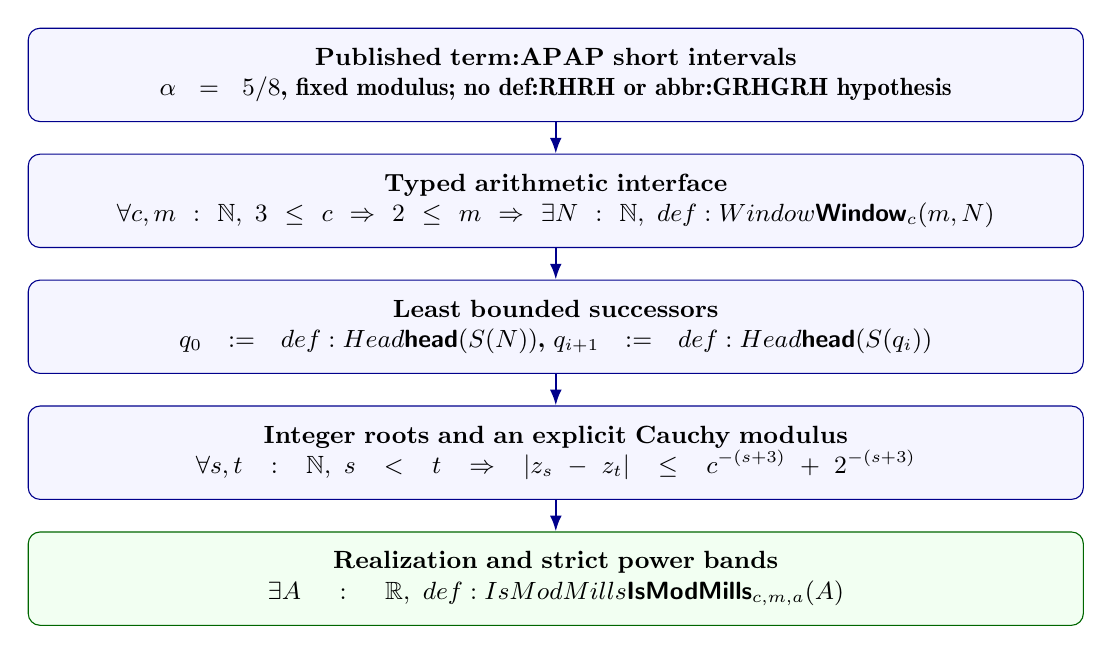
\begin{tikzpicture}[
		node distance=4mm,
		dep/.style={draw=blue!55!black,fill=blue!4,rounded corners=1.5mm,
			text width=12.9cm,align=center,font=\small,inner sep=2.5mm},
		done/.style={dep,draw=green!40!black,fill=green!5},
		flow/.style={-{Latex[length=2mm]},thick,blue!55!black}]
		\node[dep] (ap) {\textbf{Published \hyperlink{term:AP}{AP} short intervals}\\
			$\alpha=5/8$, fixed modulus; no \hyperlink{def:RH}{RH} or \hyperlink{abbr:GRH}{GRH} hypothesis};
		\node[dep,below=of ap] (win) {\textbf{Typed arithmetic interface}\\
			$\forall c,m:\N,\ 3\le c\Rightarrow2\le m\Rightarrow
			\exists N:\N,\ \hyperlink{def:Window}{\ensuremath{\textsf{Window}}}_c(m,N)$};
		\node[dep,below=of win] (seq) {\textbf{Least bounded successors}\\
			$q_0:=\hyperlink{def:Head}{\ensuremath{\textsf{head}}}(S(N))$,
			$q_{i+1}:=\hyperlink{def:Head}{\ensuremath{\textsf{head}}}(S(q_i))$};
		\node[dep,below=of seq] (code) {\textbf{Integer roots and an explicit Cauchy modulus}\\
			$\forall s,t:\N,\ s<t\Rightarrow
			|z_s-z_t|\le c^{-(s+3)}+2^{-(s+3)}$};
		\node[done,below=of code] (result) {\textbf{Realization and strict power bands}\\
			$\exists A:\R,\ \hyperlink{def:IsModMills}{\ensuremath{\textsf{IsModMills}}}_{c,m,a}(A)$};
		\draw[flow] (ap)--(win);
		\draw[flow] (win)--(seq);
		\draw[flow] (seq)--(code);
		\draw[flow] (code)--(result);
		\end{tikzpicture}
	\end{adjustbox}
	% Optional: uncomment if you use a caption
	% \caption{Your caption here}
\end{figure}

\thispagestyle{empty}


\newpage

\thispagestyle{empty}
\bigskip\tableofcontents\bigskip
\newpage\setstretch{1.2}\pagestyle{plain}\pagenumbering{arabic}
\hypersetup{pageanchor=true}

\section{Introduction}
\begin{quotation}
Mills' theorem~\cite{Mills1947} gives a real number \(\FormulaFit[\textstyle]{A>1}\) for which
\(\FormulaFit[\textstyle]{\lfloor A^{3^n}\rfloor}\) is prime for every \(\FormulaFit[\textstyle]{n\ge1}\).\\
We study the additional requirement that all these primes belong to
one prescribed reduced residue class.

For fixed \(\FormulaFit[\textstyle]{m\ge2}\) and \(\FormulaFit[\textstyle]{\operatorname{\hyperlink{abbr:gcd}{gcd}}(a,m)=1}\), the short-interval result of
Thorner--Zaman~\cite{ThornerZaman2024} supplies, for every sufficiently
large integer \(\FormulaFit[\textstyle]{p}\), a prime \(\FormulaFit[\textstyle]{r}\) satisfying
\[\FormulaFit[\displaystyle]{
p^3<r\le(p+1)^3-2,
 r\equiv a\pmod m.
}\]
Least bounded successor recursion and an explicitly convergent rational
code then yield the required constant. This is a deduction from the cited analytic input,
not a priority claim.\\

The contribution of the present exposition is the explicit interface between
that analytic input and prescribed-congruence prime chains, together with a
rational Cauchy construction and a separately bounded certificate layer.
\Cref{lem:ap-window} derives a uniform integer window;
\cref{lem:typed-window-limit,sec:typed-cauchy-proof} give its realization.
\Cref{thm:mod-finite} states exactly what the finite certificates establish.
These are different assertions, not interchangeable proofs of global existence.

The classical ten-route exposition supplies context.\\
Finite prefixes, rational inner cells, and bounded branching examples
are treated separately: their certificates verify only the stated
finite data and do not replace the analytic continuation argument.

\end{quotation}


\subsection{Historical overview: finite rules and completed numbers}\label{sec:historical-overview}
Positional notation, exact arithmetic classification, and an ontology of the
continuum have different histories. Stevin's \emph{De Thiende} (1585)
helped establish decimal arithmetic; it did not supply the later theory of
real-number completeness. The nineteenth-century constructions associated
with Dedekind and Cantor, published in 1872, gave precise accounts of real
numbers through cuts or fundamental sequences. O'Connor and Robertson
survey this development, including the distinction between Dedekind's
1858 ideas and their publication~\cite{RealNumbersHistory2005}.
These constructions explain what an exact real denotes within a theory;
they do not assert that a finite decimal display contains infinitely much
inspected information. A finite rule for a sequence and the completed
object represented by that sequence must therefore be distinguished.

Liouville's work makes the distinction especially clear. His 1851 paper
reproduces and extends notes presented in May 1844. The earlier work used
continued fractions; the later exposition also treats rapidly convergent
series and decimal constructions~\cite[pp.~133--140]{Liouville1851}.
A number specified by a finite summation rule can be transcendental: the
proof compares its rational approximants with a lower bound valid for
algebraic numbers. Thus transcendence historically arose together with
explicit approximation procedures, not as a synonym for the absence of
such procedures. The finite text of a proof can establish a statement
about every polynomial without enumerating all polynomials individually.
Whether one accepts the associated unbounded quantification is a further
foundational question, not a defect in the decimal algorithm.

The twentieth-century foundational debates also concerned different
questions. Brouwer's thesis (1907) and his critique of logical principles
(1908) initiated a systematic intuitionistic challenge to unrestricted
classical reasoning. Hilbert's programme in the 1920s sought a finitary
justification of ideal mathematics by consistency proofs; it was not
simply a proposal to replace every irrational by a terminating decimal.
Zach discusses both the programme and the competing analyses of its
finite standpoint~\cite{Zach2023}. The distinction matters here because
potentially unbounded finite calculation, primitive-recursive arithmetic,
and rejection of the completed continuum are not equivalent commitments.
The present bounded certificates address the first issue directly, but do
not settle the other two.

Turing's 1936--37 paper gave a machine account of computable
numbers~\cite{Turing1936}. His correction explicitly separated two claims:
a suitably effective shrinking rational enclosure has a digit-computable
limit in the classical, individual-existence sense, but there is no
uniform procedure converting every such enclosure into a canonical digit
machine. He then changed the representation, using overlapping intervals
and crediting Brouwer, without changing the class of computable
reals~\cite[pp.~545--546]{TuringCorrection1938}. This is an early warning
against identifying an obstruction to a particular digit representation
with an obstruction to approximation itself. Specker subsequently showed
that a computable increasing bounded rational sequence need not have a
computable limit~\cite{Specker1949}. A convergence theorem alone need not
supply a computable rate.

Bishop's \emph{Foundations of Constructive Analysis} (1967) established a
large constructive development of analysis. Modern accounts distinguish
Bishop-style mathematics, intuitionistic mathematics with choice sequences,
and recursive constructive analysis~\cite{ConstructiveSEP2022,Bauer2017}.
They must not all be equated with strict finitism or with a single
computability model. In particular, constructive mathematics allows
proofs of negation; it does not reject the ordinary elementary proof
that \(\FormulaFit[\textstyle]{\sqrt2}\) is irrational merely because that proof derives a
contradiction from an assumed rational expression.

Within number theory, Mills' 1947 theorem concerns one parameter working
for every index, whereas the computation of a least parameter is a
separate problem~\cite{Mills1947,CaldwellCheng2005}. The modern
short-interval theorem for arithmetic progressions used here adds a
prescribed congruence to the prime outputs~\cite{ThornerZaman2024}.
Saito proved irrationality of the least ordinary cubic Mills constant in
2025~\cite{Saito2025}. His subsequent paper, published in 2026, proves
its transcendence under the Density Hypothesis for the Riemann zeta
function, and hence under the Riemann Hypothesis~\cite{Saito2026}.
Unconditional transcendence of that least cubic constant remains open in
the inspected source. These arithmetic results concern exact specified
constants, not the classification of a point from a finite decimal
prefix, and they do not automatically classify our modular parameters.

\subsection{Computability, constructivity, and exact specification}\label{sec:computation-constructivity}
For the discussion in this subsection, a computable real \(\FormulaFit[\textstyle]{x}\) has one
total algorithm which, given \(\FormulaFit[\textstyle]{s:\N}\), returns a rational \(\FormulaFit[\textstyle]{E(s)}\) with
\[\FormulaFit[\displaystyle]{
 |x-E(s)|\le 2^{-s}.
}\]
The word ``one'' is essential. Separately displaying a certificate at
some fixed precision, or proving classically that an appropriate rational
exists at each precision, does not provide this algorithm. Its termination
and error bound must hold for all inputs. Conversely, computability is a
property of the represented object; constructivity concerns the proof
principles and information supporting an assertion. A classical proof
can establish computability without furnishing the program explicitly.
A nonconstructive presentation does not prove that its object is
incomputable~\cite{ConstructiveSEP2022,Bauer2017}.

\paragraph{The irrational-power example.}
The familiar two-case proof uses
\[\FormulaFit[\displaystyle]{
 t=(\sqrt2)^{\sqrt2}
   =\exp\!\left(\frac{\log 2}{\sqrt2}\right).
}\]
If \(\FormulaFit[\textstyle]{t}\) is rational, take \(\FormulaFit[\textstyle]{a=b=\sqrt2}\). If \(\FormulaFit[\textstyle]{t}\) is irrational,
take \(\FormulaFit[\textstyle]{a=t}\), \(\FormulaFit[\textstyle]{b=\sqrt2}\), so that \(\FormulaFit[\textstyle]{a^b=2}\). As presented, this
argument uses excluded middle without selecting its branch
\cite[Introduction]{ConstructiveSEP2022}. It does not demonstrate
noncomputability: \(\FormulaFit[\textstyle]{t}\) is computable by the effective operations in its
displayed expression, and the Gelfond--Schneider theorem establishes its
transcendence. A recent Lean formalization preprint includes this
application~\cite{KaratarakisWiedijk2026}; that external report is not a
kernel check of the present manuscript. Bauer also gives the direct
alternative \(\FormulaFit[\textstyle]{a=\sqrt2}\), \(\FormulaFit[\textstyle]{b=\log_2 9}\), for which \(\FormulaFit[\textstyle]{a^b=3}\);
unique prime factorization proves that \(\FormulaFit[\textstyle]{b}\) is irrational
\cite[Section~1.2]{Bauer2017}. None of these expressions is the nested
radical \(\FormulaFit[\textstyle]{\sqrt{\sqrt2}}\), which is algebraic because its fourth power is
\(\FormulaFit[\textstyle]{2}\).

\paragraph{Finite digits versus a finite defining rule.}
A finite prefix, by itself, does not establish irrationality or
transcendence of an unrestricted real point. Every nondegenerate rational
interval contains rational numbers, irrational algebraic numbers, and,
classically, transcendental numbers. This is an information limitation on
the prefix, not a contradiction in the predicates. A finite formula can
contain more information than that prefix. For example, set
\[\FormulaFit[\displaystyle]{%
\begin{gathered}
L_0:=0,\qquad
L_{N+1}:=L_N+\frac{1}{10^{(N+1)!}}\quad(N:\N),
\\[4pt]
L_N=\sum_{n=1}^{N}\frac{1}{10^{n!}}\quad(1\le N).
\end{gathered}%
}\]
The factorial gaps give the effective finite-stage bound
\[\FormulaFit[\displaystyle]{%
\begin{gathered}
\forall M,N:\N,\quad 1\le N<M\Rightarrow
\\[4pt]
0<L_M-L_N\le\frac{10}{9}\,10^{-(N+1)!}.
\end{gathered}%
}\]
Thus the finite-stage rule specifies an effective rational Cauchy code.
In the classical real interpretation, let \(\FormulaFit[\textstyle]{L}\)
denote the real represented by this code; the same upper bound controls
\(\FormulaFit[\textstyle]{L-L_N}\).
This bound supplies a terminating rational approximation algorithm: choose
\(\FormulaFit[\textstyle]{N}\) by integer comparisons until the right side is below the requested
error. It also gives rational approximations, with denominator
\(\FormulaFit[\textstyle]{10^{N!}}\), too accurate for any fixed algebraic degree, by Liouville's
inequality~\cite[Sections~3--4]{Liouville1851}. This is the standard
transcendental Liouville number, with a computable approximation rule.
Computability and transcendence therefore answer different questions.
The derivation of the displayed tail bound and the approximation algorithm
are elementary consequences of the rule, not claims that a finite digit
sample decides all algebraic relations.

\paragraph{Negation and foundations.}
To prove that a specified number is not algebraic, one may assume an
algebraic relation and derive a contradiction. Such an argument can be a
constructive proof of negation if its internal steps are constructive;
it is not automatically an application of unrestricted double-negation
elimination~\cite[Section~2]{ConstructiveSEP2022}\cite[Section~1.2]{Bauer2017}.
This observation does not certify that every transcendence proof is
constructive. Constructive formulations may also distinguish mere
non-equality from positive apartness. The logic, real representation,
and formulation of the desired conclusion must be stated before a
constructive status is claimed. Here the global proofs retain their
stated classical status; the finite certificates have the narrower
arithmetic interpretation already specified.

\subsection{Positional prefixes and congruence suffixes}\label{sec:digits-congruences}
Let \(\FormulaFit[\textstyle]{b\ge2}\) be an integer base. If a nonnegative integer has digits
\(\FormulaFit[\textstyle]{n=\sum_{j=0}^{\ell-1}d_jb^j}\), then its last \(\FormulaFit[\textstyle]{k}\) digits, padded
with zeros when necessary, specify
\[\FormulaFit[\displaystyle]{
 n\bmod b^k=\sum_{j=0}^{k-1}d_jb^j, 0\le d_j<b.
}\]
A congruence modulo \(\FormulaFit[\textstyle]{b^k}\) is therefore exactly a suffix condition.
Prescribing a prime's suffix requires compatibility with coprimality to
\(\FormulaFit[\textstyle]{b}\), apart from primes dividing \(\FormulaFit[\textstyle]{b}\). This is the finite positional
meaning of an appropriate reduced residue class. Thorner and Zaman
explicitly connect arithmetic progressions with least-significant digits
and short intervals with most-significant digits in their discussion of
prescribed-digit primes~\cite[Section~3.1, after Corollary~3.2]{ThornerZaman2024}.
Our construction prescribes congruences on prime integers, not digits of
the real parameter \(\FormulaFit[\textstyle]{A}\).

For a fractional real \(\FormulaFit[\textstyle]{0\le x<1}\), the first \(\FormulaFit[\textstyle]{k}\) digits instead
specify \(\FormulaFit[\textstyle]{D_k=\lfloor b^kx\rfloor}\) and the rational cell
\[\FormulaFit[\displaystyle]{
 \frac{D_k}{b^k}\le x<\frac{D_k+1}{b^k}.
}\]
The compatibility law is
\[\FormulaFit[\displaystyle]{
 D_{k+1}=bD_k+d_{k+1},
 D_k=\left\lfloor\frac{D_{k+1}}b\right\rfloor.
}\]
It is not the suffix compatibility law
\(\FormulaFit[\textstyle]{r_{k+1}\equiv r_k\pmod{b^k}}\). In the latter, a new high-order
integer digit is adjoined; in the former, a new low-order fractional
digit refines a real interval. Compatible residues modulo \(\FormulaFit[\textstyle]{p^k}\), for
prime \(\FormulaFit[\textstyle]{p}\), describe a \(\FormulaFit[\textstyle]{p}\)-adic integer, not in general an ordinary
real limit. For instance, the compatible residues
\(\FormulaFit[\textstyle]{1+3+\cdots+3^{k-1}}\) grow without bound in the real metric.
The shared finite digit notation does not identify the two limiting
constructions.

Likewise, the decimal identity \(\FormulaFit[\textstyle]{0.999\ldots=1}\) expresses two names
for one real, not two unequal real values. Canonical digit conventions
introduce boundary and carry problems for uniform algorithms; rational
error-bounded approximations need not decide such boundaries. Turing's
correction is a primary source for this distinction
\cite[pp.~545--546]{TuringCorrection1938}. Changing base does not convert
an unsupported real-equality decision into a finite congruence test.
The finite arithmetic interpretation is valid in each base, but it does
not by itself eliminate the logical difference between a residue, an
approximation name, and an exact real object.

\subsection{Classical, finite, and congruence layers}\label{sec:merged-scope}
The classical assertions and their finite analogues are retained together,
not substituted for one another. A finite analogue can be weaker and can
concern a different object: a finite table orbit is not the real compactness
selection theorem, and finite leaf counts are not continuum cardinality.
The proof labels \(\FormulaFit[\textstyle]{\textsf R}\), \(\FormulaFit[\textstyle]{\textsf F}\), and \(\FormulaFit[\textstyle]{\textsf M}\) identify,
respectively, the retained classical route blocks, finite route blocks,
and modular supplements. They are presentations of mathematical proofs,
not machine-checked derivations. The presentation uses typed functions,
propositions, finite data, and named analytic hypotheses. No membership-language
axiom catalogue is part of the mathematical interface. Classical real analysis
remains available for the auxiliary routes, but the main modular construction
uses an explicit convergence rate rather than arbitrary compactness.


Classical selected sequences use \(\FormulaFit[\textstyle]{n\ge1}\), whereas finite and congruence
sequences use \(\FormulaFit[\textstyle]{0\le i\le H}\). The identification is
\[\FormulaFit[\displaystyle]{
q^{\mathrm{cl}}_n=q^{\mathrm{fin}}_{n-1}\comma
c^n=c^{i+1}(n=i+1).
}\]
Thus \(\FormulaFit[\textstyle]{H}\) counts links and \(\FormulaFit[\textstyle]{H+1}\) counts primes. The modular \hyperlink{abbr:CLI}{CLI}'s
\texttt{height} counts primes: \(\FormulaFit[\textstyle]{\texttt{height}=H+1}\).
A bounded run can return fewer primes with an explicit resource status.

An outer enclosure brackets a radical endpoint or, under a separate full
continuation premise, a limiting parameter. In contrast, a finite inner
cell \(\FormulaFit[\textstyle]{[A\comma B]}\) satisfies
\[\FormulaFit[\displaystyle]{
0<A\le B\comma q_i<A^{c^{i+1}}\comma
B^{c^{i+1}}<q_i+1(0\le i\le H).
}\]
Every rational point of this cell passes the finite power tests; ordinary
real-power monotonicity gives the same conclusion for real points if the
classical layer is invoked. It is not an enclosure of a selected global
constant. The small congruence examples do not certify continuation from
their seeds. ``Modular'' means congruences on the prime values, not a
congruence on the real parameter. These are variants of Routes 1--2 and 6,
with bounded branching under Route 8 and cells under Route 10; no eleventh
route is introduced.

\subsection{Research basis and logical scope}
\hypertarget{term:PRA}{}
Historical finitism, primitive-recursive arithmetic and executable
certificate checking are distinct notions. Tait's analysis of the finite
standpoint in terms of primitive recursion is a defended foundational
position, not an uncontested definition; Zach surveys competing
analyses~\cite{Zach2023,Tait1981,Tait2012}. Leivant discusses a programming
approach to this issue~\cite{Leivant2021}. Our bounded arithmetic algorithms
are candidates for a primitive-recursive implementation, but neither a
translation of this development into \hyperlink{abbr:PRA}{PRA} nor a \hyperlink{abbr:PRA}{PRA} soundness derivation is
supplied. Termination does not imply polynomial running time.

Avigad, Gerhardy and Towsner distinguish local stability from computable
convergence rates~\cite{AvigadGerhardyTowsner2010}. We use only a finite
rational telescoping argument motivated by that distinction, stated in
\cref{fin:lem:finite-stability}. O'Connor's certified exact-real implementation
in Coq is relevant to a separate analysis layer~\cite{OConnor2008}; it is
not a verification result for the Lean source here.

Caldwell and Cheng's least cubic parameter computation is conditional on
\hyperlink{def:RH}{RH}~\cite{CaldwellCheng2005}. Elsholtz supplies unconditional explicit
large-exponent variants~\cite{Elsholtz2020}; thus one must not infer that
all explicit prime-representing parameters require \hyperlink{def:RH}{RH}. Explicit
prime-between-powers theorems include exponent \(\FormulaFit[\textstyle]{155}\) in Cully-Hugill's
published result and exponent \(\FormulaFit[\textstyle]{90}\) in Theorem~1.4 of the inspected
Cully-Hugill--Johnston preprint~\cite{CullyHugill2023,CullyHugillJohnston2026}.
These are analytic theorems, not consequences of our bounded gap tests,
and are not imported as premises of the finite certificate results. Saito's irrationality result is
also separate from finite certificate soundness~\cite{Saito2025}.



\subsection{The threshold and the computational content of this construction}\label{sec:threshold-effectivity}
The modular construction has a precise conditional algorithmic reading.
For fixed \(\FormulaFit[\textstyle]{c,m,a}\), supply an integer \(\FormulaFit[\textstyle]{N}\) satisfying the window
contract. At each stage, trial division and integer comparison decide
membership in the finite successor list, and its first entry determines
the next prime. Integer-root search then computes the rational \(\FormulaFit[\textstyle]{z_s}\)
in \cref{sec:typed-cauchy-proof}. That section proves, for the resulting
parameter \(\FormulaFit[\textstyle]{A}\),
\[\FormulaFit[\displaystyle]{
 0\le A-\iota_{\Q\R}(z_s)
 \le c^{-(s+3)}+2^{-(s+3)}\le2^{-(s+2)}.
}\]
Thus the post-window proof supplies one approximation algorithm with a
proved modulus, rather than isolated successful runs. No feasible
running-time estimate is implied: the search bounds and integer powers
can be very large.

The analytic theorem supplies existence of a suitable threshold, not a
numerical threshold in this exposition. Thorner--Zaman explicitly discuss
ineffective dependence in the small-modulus regime
\cite[Remark~1.2]{ThornerZaman2024}. Consequently the present argument
does not supply a uniform executable map from \(\FormulaFit[\textstyle]{(c,m,a)}\) to a valid
threshold and an approximation program. Within classical mathematics,
for each fixed admissible triple the existence of a finite threshold,
together with the post-window algorithm, does imply existence of a
computable parameter: a suitable integer can be hard-coded into a
program. This individual-existence conclusion must not be confused with
having identified that integer or produced the program uniformly from
the triple. Nor does ineffectivity prove that the parameter is
incomputable, or exclude a different effective construction. The least
ordinary Mills constant is a different selection problem again.

Finite inner-cell certificates make a weaker assertion. A rational point
passing every test through height \(\FormulaFit[\textstyle]{H}\) need not extend to a global prime
chain; successful finite checking supplies neither the threshold contract
nor a uniform continuation procedure. Specker's example warns in general
against inferring effective convergence merely from computable stages
and a classical limiting argument~\cite{Specker1949}. Here the modulus is
explicitly proved, so the remaining missing numerical input is identified
rather than hidden in an appeal to convergence.

\paragraph{Reading and navigation.}
Abbreviations and shortened tags are listed in \cref{tab:abbreviations}.
For the main modular argument, read the \hyperlink{term:AP}{AP} hypothesis in
\cref{sec:ap-input}, the two contracts in
\cref{lem:ap-window,lem:typed-window-limit}, and the explicit construction in
\cref{sec:typed-cauchy-proof}. The complete three-column catalogue is retained
in \cref{tab:formal-predicates}; the four-column table in
\cref{tab:all-proofs} records the classical, finite, and modular dependencies.
A blue predicate or named proof rule links to its catalogue entry.
The Dependency column contains navigation links only; mathematical details
are stated in the Formula column. A linked proof-block tag leads to its
first row, a step link to that row, and a range link to its first cited row.
Literal source listings are not rewritten as TeX hyperlinks.
The historical and foundational discussion is in
\cref{sec:historical-overview,sec:computation-constructivity,sec:digits-congruences};
\cref{sec:threshold-effectivity} states the algorithmic boundary, and
\cref{sec:conclusion-finitist,sec:conclusion-obligations} give the interpretation
and remaining proof obligations.

\section{Definitions}\label{sec:defs}

All formal predicates and notation are collected in
\cref{tab:formal-predicates}. These are mathematical specifications,
not kernel-checked declarations or a complete axiomatisation.
The table distinguishes typed objects, imported analytic facts,
inference rules, and computational status records. Hyperlinks are navigation
aids; a link does not certify the linked statement or its implementation.
The Type column gives the signature of an unapplied operator or the value
type of an applied expression. In particular, an applied predicate has type
\(\FormulaFit[\textstyle]{\hyperlink{def:Prop}{\ensuremath{\textsf{Prop}}}}\). Carriers and operations are fixed row parameters.
The typed displays are mathematical specifications, not literal Lean syntax;
their universe notation is not an implementation of Lean universes.

Universes $\FormulaFit[\textstyle]{u,v}$ are fixed parameters. Write
$\FormulaFit[\textstyle]{\mathbb B=\hyperlink{def:Fin}{\ensuremath{\textsf{Fin}}}(2)}$, $\FormulaFit[\textstyle]{\mathbb B^{<\N}=\textsf{List}(\mathbb B)}$,
and $\FormulaFit[\textstyle]{\mathbb B^j=\hyperlink{def:Fin}{\ensuremath{\textsf{Fin}}}(j)\to\mathbb B}$.
For a fixed predicate $\FormulaFit[\textstyle]{P:X\to\hyperlink{def:Prop}{\ensuremath{\textsf{Prop}}}}$, the expression
$\FormulaFit[\textstyle]{\{x:X\mid P(x)\}}$ denotes its subtype when used as a type and the
same predicate when used as an argument of a predicate-valued operation. A binder $\FormulaFit[\textstyle]{\forall x:X}$ or
$\FormulaFit[\textstyle]{\exists x:X}$ has the Lean-style meaning of quantification over terms of $\FormulaFit[\textstyle]{X}$;
$\FormulaFit[\textstyle]{P\Rightarrow Q}$ is a function type between propositions, and
$\FormulaFit[\textstyle]{\exists!x:X,\,P(x)}$ means existence together with uniqueness.
A bounded binder is notation, not an untyped domain: for $\FormulaFit[\textstyle]{S:X\to\hyperlink{def:Prop}{\ensuremath{\textsf{Prop}}}}$,
\[\FormulaFit[\displaystyle]{
\begin{gathered}
\forall x: S,\,P(x) \;:=\;\forall x:X,\ S(x)\Rightarrow P(x),
\\[4pt]
\exists x: S,\,P(x) \;:=\;\exists x:X,\ S(x)\wedge P(x).
\end{gathered}
}\]
Likewise $\FormulaFit[\textstyle]{\forall i:\N_{\le H}}$ abbreviates
$\FormulaFit[\textstyle]{\forall i:\N,\ i\le H\Rightarrow\cdots}$, whereas
$\FormulaFit[\textstyle]{\exists i\le H}$ abbreviates
$\FormulaFit[\textstyle]{\exists i:\N,\ i\le H\wedge\cdots}$.
Carrier quantification is written $\FormulaFit[\textstyle]{\forall x:X}$; bounded predicate
quantification is expanded by the preceding conventions. Subtypes retain their coercions to the
underlying carrier. In particular $\FormulaFit[\textstyle]{\Np=\{n:\N\mid 0<n\}}$ and
$\FormulaFit[\textstyle]{\R_{>a}=\{x:\R\mid a<x\}}$.

The notation $\FormulaFit[\textstyle]{\hyperlink{def:Set}{\ensuremath{\textsf{Set}}}(X)}$ means the predicate type
$\FormulaFit[\textstyle]{X\to\hyperlink{def:Prop}{\ensuremath{\textsf{Prop}}}}$, not an untyped collection. Intersections, unions,
intervals, and inclusion in the measure and branching routes are operations
on such predicates. For example,
\[\FormulaFit[\displaystyle]{
(S\cap T)(x)\iff S(x)\wedge T(x),
S\subseteq T\iff\forall x:X,\ S(x)\Rightarrow T(x).
}\]
These familiar operations are retained where mathematically useful; no
axioms of a membership-based foundational theory are asserted.
All displayed types are mathematical specifications. Only material in an
explicit Lean listing is intended as Lean syntax, and compilation is not
claimed. When the Type column names an annotation, rule, or construction,
it records a meta-level role rather than a Lean universe or a new carrier.
Such entries describe the stated proof interface, not additional axioms. Fixed row parameters are universally quantified in their stated
carrier types; names such as $\FormulaFit[\textstyle]{\hyperlink{def:Pow}{\ensuremath{\textsf{Pow}}}}$ and $\FormulaFit[\textstyle]{\hyperlink{def:Ord}{\ensuremath{\textsf{Ord}}}}$ in proof
columns refer to previously stated library facts, not additional axioms.

For measure predicates,
\(\FormulaFit[\textstyle]{\nu:\mathcal A\to\overline{\R}_{\ge0}}\),
where \(\FormulaFit[\textstyle]{\mathcal A}\) is the stated sigma-algebra;
for Lebesgue measure, \(\FormulaFit[\textstyle]{\mathcal A=\mathcal M_\mu}\).

Subscripts such as \(\FormulaFit[\textstyle]{\R_{>a}}\) denote subtypes, and \(\FormulaFit[\textstyle]{(0\comma 1)}\) denotes its real
subtype when used as a parameter type. Natural numbers start at zero; prime
classical sequences and prime-representing assertions use positive indices;
finite and modular sequences use the zero-based convention of \cref{sec:merged-scope}. The canonical
sequence \(\FormulaFit[\textstyle]{p_n}\) enumerates all primes and is distinct from a selected sequence
\(\FormulaFit[\textstyle]{q_n}\). The notation $\FormulaFit[\textstyle]{\iota_{\Q\R}:\Q\to\R}$ denotes the canonical rational embedding. The standard embeddings \(\FormulaFit[\textstyle]{\N\hookrightarrow\Z\hookrightarrow\R}\)
are understood in powers and inequalities; \(\FormulaFit[\textstyle]{\iota:\N\hookrightarrow\Z}\)
is explicit where integer primality is transported. In classical proof blocks,
unqualified sequence indices \(\FormulaFit[\textstyle]{n,j}\) range over \(\FormulaFit[\textstyle]{\Np}\); finite indices
range only over their displayed bounds. Mathematical finite lists $\FormulaFit[\textstyle]{q}$ may
be padded to functions $\FormulaFit[\textstyle]{\N\to\N}$; all finite assertions inspect only
$\FormulaFit[\textstyle]{i\le H}$. The corresponding Lean datum is the restriction
$\FormulaFit[\textstyle]{\lambda i:\hyperlink{def:Fin}{\ensuremath{\textsf{Fin}}}(H+1),\,q(i.\textsf{val})}$, so padding values
have no mathematical effect. A positive-index sequence may be
encoded in Lean as a total natural-index function with a \(\FormulaFit[\textstyle]{0<n}\) guard;
its value at zero is immaterial. Natural-valued sequences are coerced
pointwise when a real-valued predicate is applied. Fields and rings in the
supporting rows mean carriers with fixed operations, not additional sorts
named by the predicates \(\FormulaFit[\textstyle]{\hyperlink{def:Field}{\ensuremath{\textsf{Field}}}}\) and \(\FormulaFit[\textstyle]{\hyperlink{def:CommutativeRing}{\ensuremath{\textsf{CommutativeRing}}}}\).

The zeta specification includes its usual meromorphic continuation, with its
only pole at \(\FormulaFit[\textstyle]{1}\), and the auxiliary total-function convention \(\FormulaFit[\textstyle]{\zeta(1)=0}\).
Zero statements exclude the pole. The symbol \(\FormulaFit[\textstyle]{\mu}\) is Lebesgue outer measure;
no countable-additivity claim on all subsets of \(\FormulaFit[\textstyle]{\R}\) is intended.
On bounded measurable sets its value is finite; when \(\FormulaFit[\textstyle]{\mu(F_m)}\)
appears in real arithmetic or in \(\FormulaFit[\textstyle]{\hyperlink{def:Conv}{\ensuremath{\textsf{Conv}}}}\), it denotes the unique
nonnegative real whose embedding is that extended measure value. The floor
specification is not a uniform computability assertion for arbitrary reals.
The fixed-base and fixed-exponent parameter families do not imply a null-set
statement for an uncountable union over their parameters. Iterated logarithms
are used only on the recursively specified domains \(\FormulaFit[\textstyle]{D_n}\).

\phantomsection\label{sec:defs-prim-types}
\phantomsection\label{sec:defs-prim-ops}
\phantomsection\label{sec:defs-prim-pred}
\phantomsection\label{sec:defs-mills}
\phantomsection\label{sec:defs-kanw}
\phantomsection\label{sec:defs-ore}
\phantomsection\label{sec:defs-polygap}
\phantomsection\label{sec:defs-rm}
\phantomsection\label{sec:defs-theta}
\phantomsection\label{sec:defs-iter}

\begingroup
\scriptsize
\renewcommand{\arraystretch}{1.2}
\setlength{\tabcolsep}{3pt}
\begingroup
\SplitTableCaption{All formal predicates and notation.}\label{tab:formal-predicates}\label{tab:proof-definitions}\label{tab:definitions}\label{tab:euclid-definitions}\label{tab:slope-definitions}\label{tab:power-bound-definitions}\label{tab:mills-squeeze-definitions}\label{tab:axioms}\label{tab:algorithms}\label{tab:systems}
\par\nobreak
\noindent
\begin{tabular}{|@{}p{0.19251\linewidth}|p{0.16845\linewidth}|p{0.53904\linewidth}|}\hline
{\textbf{\large{Predicate}}} & {\textbf{\large{Type}}} & {\textbf{\large{Formula}}}\\
\hline
{\defitem{Prop}{\phantomsection\label{def:prop}\label{type:PropType}\label{asser:prop-axioms}\(\FormulaFit[\textstyle]{\textsf{Prop}}\)}} & {\(\FormulaFit[\textstyle]{\textsf{Sort}_{1}}\)} & {\(\FormulaFit[\textstyle]{

\forall P\comma Q:\hyperlink{def:Prop}{\ensuremath{\textsf{Prop}}}\comma (P\wedge Q)\comma (P\vee Q)\comma (P\Rightarrow Q)\comma \neg P:\hyperlink{def:Prop}{\ensuremath{\textsf{Prop}}}
\allowbreak  \forall X:\hyperlink{def:Universe}{\ensuremath{\textsf{Type}}}\comma \ \forall P:X\to\allowbreak \hyperlink{def:Prop}{\ensuremath{\textsf{Prop}}}\comma (
\quad 
\forall x:X\comma P(x))\comma (\exists x:X\comma P(x)):\hyperlink{def:Prop}{\ensuremath{\textsf{Prop}}}

}\)}\\
\hline
\end{tabular}%
\par\setlength{\parskip}{0pt}\nointerlineskip
\noindent
\begin{tabular}{|@{}p{0.19251\linewidth}|p{0.16845\linewidth}|p{0.53904\linewidth}|}\hline
{\defitem{Nat}{\phantomsection\label{def:nat}\label{type:NatType}\label{asser:nat-axioms}\(\FormulaFit[\textstyle]{\mathbb{N}}\)}} & {\(\FormulaFit[\textstyle]{\hyperlink{def:Universe}{\textsf{Type}}}\)} & {\(\FormulaFit[\textstyle]{\hyperlink{def:Peano}{\ensuremath{\textsf{Peano}}}(\mathbb{N}\comma  0\comma  \hyperlink{def:Successor}{\mathsf{succ}})}\)}\\
\hline
\end{tabular}%
\par\setlength{\parskip}{0pt}\nointerlineskip
\noindent
\begin{tabular}{|@{}p{0.19251\linewidth}|p{0.16845\linewidth}|p{0.53904\linewidth}|}\hline
{\defitem{IntType}{\phantomsection\label{def:int}\label{type:IntType}\label{asser:int-axioms}\(\FormulaFit[\textstyle]{\mathbb{Z}}\)}} & {\(\FormulaFit[\textstyle]{\hyperlink{def:Universe}{\textsf{Type}}}\)} & {\(\FormulaFit[\textstyle]{\hyperlink{def:IntegralDomain}{\ensuremath{\textsf{IntegralDomain}}}(\mathbb{Z}\comma  +\comma  \cdot\comma  0\comma 
1) \wedge \hyperlink{def:Initial}{\ensuremath{\textsf{Initial}}}(\mathbb{Z}) \wedge \hyperlink{def:Characteristic}{\mathsf{char}}(\mathbb{Z})
= 0}\)}\\
\hline
\end{tabular}%
\par\setlength{\parskip}{0pt}\nointerlineskip
\noindent
\begin{tabular}{|@{}p{0.19251\linewidth}|p{0.16845\linewidth}|p{0.53904\linewidth}|}\hline
{\defitem{RealType}{\phantomsection\label{def:real}\label{type:RealType}\label{asser:real-axioms}\(\FormulaFit[\textstyle]{\mathbb{R}}\)}} & {\(\FormulaFit[\textstyle]{\hyperlink{def:Universe}{\textsf{Type}}}\)} & {\(\FormulaFit[\textstyle]{

\hyperlink{def:Field}{\ensuremath{\textsf{Field}}}(\mathbb{R}\comma  +\comma  \cdot\comma  0\comma  1) \wedge \hyperlink{def:LinearOrder}{\ensuremath{\textsf{LinearOrder}}}(\mathbb{R}\comma  <) \allowbreak 
 \wedge \hyperlink{def:OrderCompatible}{\ensuremath{\textsf{OrderCompatible}}}(+\comma  \cdot\comma  <)
\quad 
\wedge \hyperlink{def:DedekindComplete}{\ensuremath{\textsf{DedekindComplete}}}(\mathbb{R}\comma  <)

}\)}\\
\hline
\end{tabular}%
\par\setlength{\parskip}{0pt}\nointerlineskip
\noindent
\begin{tabular}{|@{}p{0.19251\linewidth}|p{0.16845\linewidth}|p{0.53904\linewidth}|}\hline
{\defitem{ComplexType}{\phantomsection\label{def:complex}\label{type:ComplexType}\label{asser:complex-axioms}\(\FormulaFit[\textstyle]{\mathbb{C}}\)}} & {\(\FormulaFit[\textstyle]{\hyperlink{def:Universe}{\textsf{Type}}}\)} & {\(\FormulaFit[\textstyle]{\hyperlink{def:AlgebraicClosure}{\ensuremath{\textsf{AlgebraicClosure}}}(\mathbb{C}\comma 
\mathbb{R}) \wedge \hyperlink{def:ContainsBase}{\ensuremath{\textsf{ContainsBase}}}(\R,\C)}\)}\\
\hline
\end{tabular}%
\par\setlength{\parskip}{0pt}\nointerlineskip
\noindent
\begin{tabular}{|@{}p{0.19251\linewidth}|p{0.16845\linewidth}|p{0.53904\linewidth}|}\hline
{\defitem{Exp}{\phantomsection\label{def:exp-prim}\label{type:ExpPrimType}\label{asser:exp-prim-axioms}\(\FormulaFit[\textstyle]{\exp}\)}} & {\(\FormulaFit[\textstyle]{\mathbb{R} \to\allowbreak  \mathbb{R}}\)} & {\(\FormulaFit[\textstyle]{
\exp(0) = 1 \wedge \bigl(\forall x : \mathbb{R}\comma \ \exp'(x) = \exp(x)\bigr) \allowbreak 
 \wedge \bigl(\forall x\comma  y : \mathbb{R}\comma \ \exp(x+y) = \exp(x)\cdot\exp(y)\bigr)
}\)}\\
\hline
\end{tabular}%
\par\setlength{\parskip}{0pt}\nointerlineskip
\noindent
\begin{tabular}{|@{}p{0.19251\linewidth}|p{0.16845\linewidth}|p{0.53904\linewidth}|}\hline
{\defitem{Log}{\phantomsection\label{def:log-prim}\label{type:LogPrimType}\label{asser:log-prim-axioms}\(\FormulaFit[\textstyle]{\log}\)}} & {\(\FormulaFit[\textstyle]{\mathbb{R}_{>0} \to\allowbreak  \mathbb{R}}\)} & {\(\FormulaFit[\textstyle]{\bigl(\forall x : \mathbb{R}\comma \ \log(\exp(x))
= x\bigr) \wedge \bigl(\forall y : \mathbb{R}_{>0}\comma \ \exp(\log(y)) = y
\bigr)}\)}\\
\hline
\end{tabular}%
\par\setlength{\parskip}{0pt}\nointerlineskip
\noindent
\begin{tabular}{|@{}p{0.19251\linewidth}|p{0.16845\linewidth}|p{0.53904\linewidth}|}\hline
{\defitem{Exp2}{\phantomsection\label{def:exp2-prim}\label{type:Exp2PrimType}\label{asser:exp2-prim-axioms}\(\FormulaFit[\textstyle]{\exp_2}\)}} & {\(\FormulaFit[\textstyle]{\mathbb{R} \to\allowbreak  \mathbb{R}}\)} & {\(\FormulaFit[\textstyle]{\forall x : \mathbb{R}\comma \ \exp_2(x) = \exp(x \log 2)}\)}\\
\hline
\end{tabular}%
\par\setlength{\parskip}{0pt}\nointerlineskip
\noindent
\begin{tabular}{|@{}p{0.19251\linewidth}|p{0.16845\linewidth}|p{0.53904\linewidth}|}\hline
{\defitem{Log2}{\phantomsection\label{def:log2-prim}\label{type:Log2PrimType}\label{asser:log2-prim-axioms}\(\FormulaFit[\textstyle]{\log_2}\)}} & {\(\FormulaFit[\textstyle]{\mathbb{R}_{>0} \to\allowbreak  \mathbb{R}}\)} & {\(\FormulaFit[\textstyle]{\bigl(\forall x : \mathbb{R}\comma \ \log_2(\exp_2(x))
= x\bigr) \wedge \bigl(\forall y : \mathbb{R}_{>0}\comma \ \exp_2(\log_2(y)) = y
\bigr)}\)}\\
\hline
\end{tabular}%
\par\setlength{\parskip}{0pt}\nointerlineskip
\noindent
\begin{tabular}{|@{}p{0.19251\linewidth}|p{0.16845\linewidth}|p{0.53904\linewidth}|}\hline
{\defitem{LogBase}{\phantomsection\label{def:logc-prim}\label{type:LogCPrimType}\label{asser:logc-prim-axioms}\(\FormulaFit[\textstyle]{\log_c}\)}} & {\(\FormulaFit[\textstyle]{\mathbb{R}_{>0} \to\allowbreak  \mathbb{R}}\)} & {\(\FormulaFit[\textstyle]{\forall c : \mathbb{R}_{>0\comma  \neq 1}\comma \ \forall x : \mathbb{R}_{>0}\comma \ \log_c(x) = \frac{\log x}{\log c}}\)}\\
\hline
\end{tabular}%
\par\setlength{\parskip}{0pt}\nointerlineskip
\noindent
\begin{tabular}{|@{}p{0.19251\linewidth}|p{0.16845\linewidth}|p{0.53904\linewidth}|}\hline
{\defitem{Zeta}{\phantomsection\label{def:zeta}\label{type:ZetaType}\label{asser:zeta-axioms}\(\FormulaFit[\textstyle]{\zeta}\)}} & {\(\FormulaFit[\textstyle]{\mathbb{C} \to\allowbreak  \mathbb{C}}\)} & {\(\FormulaFit[\textstyle]{\forall s : \mathbb{C}\comma \ \Re(s) > 1 \Rightarrow
	\zeta(s) = \sum_{n:\mathbb{N}_{>0}} n^{-s}}\)}\\
\hline
\end{tabular}%
\par\setlength{\parskip}{0pt}\nointerlineskip
\noindent
\begin{tabular}{|@{}p{0.19251\linewidth}|p{0.16845\linewidth}|p{0.53904\linewidth}|}\hline
{\defitem{RealPart}{\phantomsection\label{def:re}\label{type:ReType}\label{asser:re-axioms}\(\FormulaFit[\textstyle]{\Re}\)}} & {\(\FormulaFit[\textstyle]{\mathbb{C} \to\allowbreak  \mathbb{R}}\)} & {\(\FormulaFit[\textstyle]{\forall a\comma  b : \mathbb{R}\comma \ \Re(a + bi) = a}\)}\\
\hline
\end{tabular}%
\par\setlength{\parskip}{0pt}\nointerlineskip
\noindent
\begin{tabular}{|@{}p{0.19251\linewidth}|p{0.16845\linewidth}|p{0.53904\linewidth}|}\hline
{\defitem{Continuous}{\phantomsection\label{def:continuous}\label{type:ContinuousType}\label{asser:continuous-axioms}\(\FormulaFit[\textstyle]{\textsf{Continuous}}\)}} & {\(\FormulaFit[\textstyle]{(\mathbb{R} \to\allowbreak 
\mathbb{R}) \to\allowbreak  \hyperlink{def:Prop}{\textsf{Prop}}}\)} & {\(\FormulaFit[\textstyle]{

\forall f : \mathbb{R} \to\allowbreak  \mathbb{R}\comma \ \hyperlink{def:Continuous}{\ensuremath{\textsf{Continuous}}}(f) :\iff \allowbreak 
 \forall x : \mathbb{R}\comma \ \forall \varepsilon : \mathbb{R}_{>0}\comma \ \exists  \delta : \mathbb{R}_{>0}\comma \
\quad 
\forall y : \mathbb{R}\comma  \allowbreak 
 |y - x| < \delta \Rightarrow |f(y) - f(x)| < \varepsilon

}\)}\\
\hline
\end{tabular}%
\par\setlength{\parskip}{0pt}\nointerlineskip
\noindent
\begin{tabular}{|@{}p{0.19251\linewidth}|p{0.16845\linewidth}|p{0.53904\linewidth}|}\hline
{\defitem{EventuallyIncreasing}{\phantomsection\label{def:eventually-increasing}\label{type:EventuallyIncreasingType}\label{asser:eventually-increasing-axioms}\(\FormulaFit[\textstyle]{\textsf{EventuallyIncreasing}}\)}} & {\(\FormulaFit[\textstyle]{(
\mathbb{R} \to\allowbreak  \mathbb{R}) \to\allowbreak  \hyperlink{def:Prop}{\textsf{Prop}}}\)} & {\(\FormulaFit[\textstyle]{

\forall f : \mathbb{R} \to\allowbreak  \mathbb{R}\comma \ \hyperlink{def:EventuallyIncreasing}{\ensuremath{\textsf{EventuallyIncreasing}}}(f) :\iff \allowbreak 
 \exists  N : \mathbb{R}\comma \ \forall x\comma  y : \mathbb{R}\comma \ N < x < y
\quad 
\Rightarrow f(x) < f(y)

}\)}\\
\hline
\end{tabular}%
\par\setlength{\parskip}{0pt}\nointerlineskip
\noindent
\begin{tabular}{|@{}p{0.19251\linewidth}|p{0.16845\linewidth}|p{0.53904\linewidth}|}\hline
{\defitem{Bijective}{\phantomsection\label{def:bijective}\label{type:BijectiveType}\label{asser:bijective-axioms}\(\FormulaFit[\textstyle]{\textsf{Bijective}}\)}} & {\(\FormulaFit[\textstyle]{

\forall \alpha\comma  \beta :
\hyperlink{def:Universe}{\textsf{Type}}\comma \ (\alpha \to\allowbreak  \beta)
\quad 
\to\allowbreak  \hyperlink{def:Prop}{\textsf{Prop}}

}\)} & {\(\FormulaFit[\textstyle]{

\forall \alpha\comma  \beta : \hyperlink{def:Universe}{\ensuremath{\textsf{Type}}}\comma \ \forall f : \alpha \to\allowbreak  \beta\comma \ \hyperlink{def:Bijective}{\ensuremath{\textsf{Bijective}}}(f) :\iff \allowbreak 
 \bigl(\forall x\comma  y : \alpha\comma \ f(x) = f(y)
\quad 
\Rightarrow x = y\bigr) \allowbreak 
 \wedge \bigl(\forall y : \beta\comma \ \exists  x : \alpha\comma \ f(x) = y\bigr)

}\)}\\
\hline
\end{tabular}%
\par\setlength{\parskip}{0pt}\nointerlineskip
\noindent
\begin{tabular}{|@{}p{0.19251\linewidth}|p{0.16845\linewidth}|p{0.53904\linewidth}|}\hline
{\defitem{LebesgueOuter}{\phantomsection\label{def:measure}\label{type:MeasureType}\label{asser:measure-axioms}\(\FormulaFit[\textstyle]{\mu}\)}} & {\(\FormulaFit[\textstyle]{(\mathbb{R} \to\allowbreak  \hyperlink{def:Prop}{\textsf{Prop}}) \to\allowbreak 
	\mathbb{R}_{\geq 0}^{\mathrm{ext}}}\)} & {\(\FormulaFit[\textstyle]{\hyperlink{def:LebesgueOuterMeasure}{\ensuremath{\textsf{LebesgueOuterMeasure}}}(\mu\comma  \mathbb{R})}\)}\\
\hline
\end{tabular}%
\par\setlength{\parskip}{0pt}\nointerlineskip
\noindent
\begin{tabular}{|@{}p{0.19251\linewidth}|p{0.16845\linewidth}|p{0.53904\linewidth}|}\hline
{\defitem{Int}{\phantomsection\label{def:interior}\label{type:InteriorType}\label{asser:interior-axioms}\(\FormulaFit[\textstyle]{\textsf{Int}}\)}} & {\(\FormulaFit[\textstyle]{(\mathbb{R} \to\allowbreak  \hyperlink{def:Prop}{\textsf{Prop}})
\to\allowbreak  (\mathbb{R} \to\allowbreak  \hyperlink{def:Prop}{\textsf{Prop}})}\)} & {\(\FormulaFit[\textstyle]{

\forall S : \mathbb{R} \to\allowbreak  \hyperlink{def:Prop}{\ensuremath{\textsf{Prop}}}\comma \ \hyperlink{def:Int}{\ensuremath{\textsf{Int}}}(S) \subseteq S \wedge \hyperlink{def:IsOpen}{\ensuremath{\textsf{IsOpen}}}(\hyperlink{def:Int}{\ensuremath{\textsf{Int}}}(S)) \allowbreak 
 \wedge \forall U : \mathbb{R} \to\allowbreak  \hyperlink{def:Prop}{\ensuremath{\textsf{Prop}}}\comma \ \bigl(\hyperlink{def:IsOpen}{\ensuremath{\textsf{IsOpen}}}(U)
\quad 
\wedge U \subseteq S\bigr) \Rightarrow U \subseteq \hyperlink{def:Int}{\ensuremath{\textsf{Int}}}(S)

}\)}\\
\hline
\end{tabular}%
\par\setlength{\parskip}{0pt}\nointerlineskip
\noindent
\begin{tabular}{|@{}p{0.19251\linewidth}|p{0.16845\linewidth}|p{0.53904\linewidth}|}\hline
{\defitem{cl}{\phantomsection\label{def:closure}\label{type:ClosureType}\label{asser:closure-axioms}\(\FormulaFit[\textstyle]{\textsf{cl}}\)}} & {\(\FormulaFit[\textstyle]{

(\mathbb{R} \to\allowbreak  \hyperlink{def:Prop}{\textsf{Prop}}) \to\allowbreak 
( \mathbb{R}
\quad 
\to\allowbreak  \hyperlink{def:Prop}{\textsf{Prop}})

}\)} & {\(\FormulaFit[\textstyle]{

\forall S : \mathbb{R} \to\allowbreak  \hyperlink{def:Prop}{\ensuremath{\textsf{Prop}}}\comma \ S \subseteq \hyperlink{def:cl}{\ensuremath{\textsf{cl}}}(S) \wedge \hyperlink{def:IsClosed}{\ensuremath{\textsf{IsClosed}}}(\hyperlink{def:cl}{\ensuremath{\textsf{cl}}}(S)) \allowbreak 
 \wedge \forall F : \mathbb{R} \to\allowbreak  \hyperlink{def:Prop}{\ensuremath{\textsf{Prop}}}\comma \ \bigl(\hyperlink{def:IsClosed}{\ensuremath{\textsf{IsClosed}}}(F)
\quad 
\wedge S \subseteq F\bigr) \Rightarrow \hyperlink{def:cl}{\ensuremath{\textsf{cl}}}(S) \subseteq F

}\)}\\
\hline
\end{tabular}%
\par\setlength{\parskip}{0pt}\nointerlineskip
\noindent
\begin{tabular}{|@{}p{0.19251\linewidth}|p{0.16845\linewidth}|p{0.53904\linewidth}|}\hline
{\defitem{Prime}{\phantomsection\label{def:prime}\label{type:PrimeType}\label{asser:prime}\(\FormulaFit[\textstyle]{\textsf{Prime}}\)}} & {\(\FormulaFit[\textstyle]{\mathbb{N} \to\allowbreak  \hyperlink{def:Prop}{\textsf{Prop}}}\)} & {\(\FormulaFit[\textstyle]{\forall p : \mathbb{N}\comma \ \hyperlink{def:Prime}{\ensuremath{\textsf{Prime}}}(p) :\iff (p
\geq 2) \wedge \bigl(\forall d : \mathbb{N}\comma \ (d \geq 2 \wedge d \mid p)
\Rightarrow d = p\bigr)}\)}\\
\hline
\end{tabular}%
\par\setlength{\parskip}{0pt}\nointerlineskip
\noindent
\begin{tabular}{|@{}p{0.19251\linewidth}|p{0.16845\linewidth}|p{0.53904\linewidth}|}\hline
{\defitem{Nat.Prime}{\(\FormulaFit[\textstyle]{\textsf{Nat.Prime}(p)}\)}} & {\(\FormulaFit[\textstyle]{\hyperlink{def:Prop}{\textsf{Prop}}}\)} & {\(\FormulaFit[\textstyle]{p:\N\comma\hyperlink{def:Nat.Prime}{\ensuremath{\textsf{Nat.Prime}}}(p)\iff\hyperlink{def:Prime}{\ensuremath{\textsf{Prime}}}(p)}\)}\\
\hline
\end{tabular}%
\par\setlength{\parskip}{0pt}\nointerlineskip
\noindent
\begin{tabular}{|@{}p{0.19251\linewidth}|p{0.16845\linewidth}|p{0.53904\linewidth}|}\hline
{\defitem{floor}{\phantomsection\label{def:floor}\label{type:FloorType}\label{asser:floor}\(\FormulaFit[\textstyle]{\textsf{floor}}\)}} & {\(\FormulaFit[\textstyle]{\mathbb{R} \to\allowbreak  \mathbb{Z}}\)} & {\(\FormulaFit[\textstyle]{\forall x : \mathbb{R}\comma \ \forall n : \mathbb{Z}\comma \
\hyperlink{def:floor}{\ensuremath{\textsf{floor}}}(x) = n \iff (n \leq x < n + 1)}\)}\\
\hline
\end{tabular}%
\par\setlength{\parskip}{0pt}\nointerlineskip
\noindent
\begin{tabular}{|@{}p{0.19251\linewidth}|p{0.16845\linewidth}|p{0.53904\linewidth}|}\hline
{\defitem{PrimeZ}{\phantomsection\label{def:primez}\label{type:PrimeZType}\label{asser:primez}\(\FormulaFit[\textstyle]{\textsf{Prime}_{\Z}}\)}} & {\(\FormulaFit[\textstyle]{\Z\to\allowbreak \hyperlink{def:Prop}{\textsf{Prop}}}\)} & {\(\FormulaFit[\textstyle]{\forall m:\Z\comma  \hyperlink{def:PrimeZ}{\ensuremath{\textsf{Prime}_{\Z}}}(m)\iff
\exists p:\N\comma \ \hyperlink{def:Prime}{\ensuremath{\textsf{Prime}}}(p)\wedge m=\iota(p)\comma }\)}\\
\hline
\end{tabular}%
\par\setlength{\parskip}{0pt}\nointerlineskip
\noindent
\begin{tabular}{|@{}p{0.19251\linewidth}|p{0.16845\linewidth}|p{0.53904\linewidth}|}\hline
{\defitem{PSeq}{\phantomsection\label{def:pseq}\label{type:PSeqType}\label{asser:pseq}\(\FormulaFit[\textstyle]{\textsf{PSeq}}\)}} & {\(\FormulaFit[\textstyle]{(\Np \to\allowbreak  \mathbb{N})
\to\allowbreak  \hyperlink{def:Prop}{\textsf{Prop}}}\)} & {\(\FormulaFit[\textstyle]{

\forall p : \Np \to\allowbreak  \mathbb{N}\comma \ \hyperlink{def:PSeq}{\ensuremath{\textsf{PSeq}}}(p) :\iff \bigl(p_1 = 2\bigr) \allowbreak 
 \wedge \bigl(\forall n : \mathbb{N}_{\geq 1}\comma \ \hyperlink{def:Prime}{\ensuremath{\textsf{Prime}}}(p_n)\bigr) \allowbreak 
 \wedge \bigl(
\quad 
\forall n : \mathbb{N}_{\geq 1}\comma \ p_n < p_{n+1}\bigr) \allowbreak 
 \wedge\bigl(\forall r:\N\comma \ \hyperlink{def:Prime}{\ensuremath{\textsf{Prime}}}(r)\Rightarrow\exists n\ge1\comma \ p_n=r\bigr)

}\)}\\
\hline
\end{tabular}%
\par\setlength{\parskip}{0pt}\nointerlineskip
\noindent
\begin{tabular}{|@{}p{0.19251\linewidth}|p{0.16845\linewidth}|p{0.53904\linewidth}|}\hline
{\defitem{IsMills}{\phantomsection\label{def:ismills}\label{type:IsMillsType}\label{asser:ismills}\(\FormulaFit[\textstyle]{\textsf{IsMills}}\)}} & {\(\FormulaFit[\textstyle]{\mathbb{R} \to\allowbreak  \textsf{
Prop}}\)} & {\(\FormulaFit[\textstyle]{\forall A : \mathbb{R}\comma \ \hyperlink{def:IsMills}{\ensuremath{\textsf{IsMills}}}(A) :\iff
(A > 1) \wedge \bigl(\forall n : \mathbb{N}_{\geq 1}\comma \ \hyperlink{def:PrimeZ}{\ensuremath{\textsf{Prime}_{\Z}}}(\hyperlink{def:floor}{\ensuremath{\textsf{floor}}}(A^{3^{n}}))\bigr)}\)}\\
\hline
\end{tabular}%
\par\setlength{\parskip}{0pt}\nointerlineskip
\noindent
\begin{tabular}{|@{}p{0.19251\linewidth}|p{0.16845\linewidth}|p{0.53904\linewidth}|}\hline
{\defitem{IsMinMills}{\phantomsection\label{def:isminmills}\label{type:IsMinMillsType}\label{asser:isminmills}\(\FormulaFit[\textstyle]{\textsf{IsMinMills}}\)}} & {\(\FormulaFit[\textstyle]{\mathbb{R} \to\allowbreak 
\hyperlink{def:Prop}{\textsf{Prop}}}\)} & {\(\FormulaFit[\textstyle]{\forall A : \mathbb{R}\comma \ \hyperlink{def:IsMinMills}{\ensuremath{\textsf{IsMinMills}}}(A)
:\iff \hyperlink{def:IsMills}{\ensuremath{\textsf{IsMills}}}(A) \wedge \bigl(\forall B : \mathbb{R}\comma \ \hyperlink{def:IsMills}{\ensuremath{\textsf{IsMills}}}(B) \Rightarrow A \leq B\bigr)}\)}\\
\hline
\end{tabular}%
\par\setlength{\parskip}{0pt}\nointerlineskip
\noindent
\begin{tabular}{|@{}p{0.19251\linewidth}|p{0.16845\linewidth}|p{0.53904\linewidth}|}\hline
{\defitem{MillsRec}{\phantomsection\label{def:millsrec}\label{type:MillsRecType}\label{asser:millsrec}\(\FormulaFit[\textstyle]{\textsf{MillsRec}}\)}} & {\(\FormulaFit[\textstyle]{(\Np \to\allowbreak 
\mathbb{N}) \to\allowbreak  \hyperlink{def:Prop}{\textsf{Prop}}}\)} & {\(\FormulaFit[\textstyle]{\forall q : \Np \to\allowbreak  \mathbb{N}\comma \ \hyperlink{def:MillsRec}{\ensuremath{\textsf{MillsRec}}}(q) :\iff \forall n : \mathbb{N}_{\geq 1}\comma \ q_n^{3} < q_{n+1} <
(q_n + 1)^{3} - 1}\)}\\
\hline
\end{tabular}%
\par\setlength{\parskip}{0pt}\nointerlineskip
\noindent
\begin{tabular}{|@{}p{0.19251\linewidth}|p{0.16845\linewidth}|p{0.53904\linewidth}|}\hline
{\defitem{UV}{\phantomsection\label{def:uv}\label{type:UVType}\label{asser:uv}\(\FormulaFit[\textstyle]{\textsf{UV}}\)}} & {\(\FormulaFit[\textstyle]{

(\Np \to\allowbreak  \mathbb{N})
\times\allowbreak  (\Np \to\allowbreak  \mathbb{R}) \times\allowbreak  (\Np
\quad 
\to\allowbreak  \mathbb{R}
) \to\allowbreak  \hyperlink{def:Prop}{\textsf{Prop}}

}\)} & {\(\FormulaFit[\textstyle]{

\forall q : \Np \to\allowbreak  \mathbb{N}\comma \ \forall u\comma  v : \Np \to\allowbreak  \mathbb{R}\comma \ \hyperlink{def:UV}{\ensuremath{\textsf{UV}}}(q\comma  u\comma  v) :\iff \allowbreak 
 \forall n : \mathbb{N}_{\geq 1}\comma \ \bigl(u_n = q_n^{3^{-n}}\bigr)
\quad 
\wedge \bigl(v_n = (q_n + 1)^{3^{-n}}\bigr)

}\)}\\
\hline
\end{tabular}%
\par\setlength{\parskip}{0pt}\nointerlineskip
\noindent
\begin{tabular}{|@{}p{0.19251\linewidth}|p{0.16845\linewidth}|p{0.53904\linewidth}|}\hline
{\defitem{IsKuipers}{\phantomsection\label{def:iskuipers}\label{type:IsKuipersType}\label{asser:iskuipers}\(\FormulaFit[\textstyle]{\textsf{IsKuipers}}\)}} & {\(\FormulaFit[\textstyle]{\mathbb{N}_{\geq 3}
\times\allowbreak  \mathbb{R} \to\allowbreak  \hyperlink{def:Prop}{\textsf{Prop}}}\)} & {\(\FormulaFit[\textstyle]{

\forall c : \mathbb{N}_{\geq 3}\comma \ \forall A : \mathbb{R}\comma \ \hyperlink{def:IsKuipers}{\ensuremath{\textsf{IsKuipers}}}(c\comma  A) :\iff \allowbreak 
 (A > 1) \wedge \bigl(
\quad 
\forall n : \mathbb{N}_{\geq 1}\comma \ \hyperlink{def:PrimeZ}{\ensuremath{\textsf{Prime}_{\Z}}}(\hyperlink{def:floor}{\ensuremath{\textsf{floor}}}(A^{c^{n}}))\bigr)

}\)}\\
\hline
\end{tabular}%
\par\setlength{\parskip}{0pt}\nointerlineskip
\noindent
\begin{tabular}{|@{}p{0.19251\linewidth}|p{0.16845\linewidth}|p{0.53904\linewidth}|}\hline
{\defitem{IsAnsari}{\phantomsection\label{def:isansari}\label{type:IsAnsariType}\label{asser:isansari}\(\FormulaFit[\textstyle]{\textsf{IsAnsari}}\)}} & {\(\FormulaFit[\textstyle]{\mathbb{R}_{>8/3}
\times\allowbreak  \mathbb{R} \to\allowbreak  \hyperlink{def:Prop}{\textsf{Prop}}}\)} & {\(\FormulaFit[\textstyle]{

\forall c : \mathbb{R}_{>8/3}\comma \ \forall A : \mathbb{R}\comma \ \hyperlink{def:IsAnsari}{\ensuremath{\textsf{IsAnsari}}}(c\comma  A) :\iff \allowbreak 
 (A > 1) \wedge \bigl(
\quad 
\forall n : \mathbb{N}_{\geq 1}\comma \ \hyperlink{def:PrimeZ}{\ensuremath{\textsf{Prime}_{\Z}}}(\hyperlink{def:floor}{\ensuremath{\textsf{floor}}}(A^{c^{n}}))\bigr)

}\)}\\
\hline
\end{tabular}%
\par\setlength{\parskip}{0pt}\nointerlineskip
\noindent
\begin{tabular}{|@{}p{0.19251\linewidth}|p{0.16845\linewidth}|p{0.53904\linewidth}|}\hline
{\defitem{IsWright}{\phantomsection\label{def:iswright}\label{type:IsWrightType}\label{asser:iswright}\(\FormulaFit[\textstyle]{\textsf{IsWright}}\)}} & {\(\FormulaFit[\textstyle]{\mathbb{R} \to\allowbreak  \hyperlink{def:Prop}{\textsf{Prop}}}\)} & {\(\FormulaFit[\textstyle]{\forall A : \mathbb{R}\comma \ \hyperlink{def:IsWright}{\ensuremath{\textsf{IsWright}}}(A) :\iff
(A > 1) \wedge \bigl(\forall n : \mathbb{N}_{\geq 1}\comma \ \hyperlink{def:PrimeZ}{\ensuremath{\textsf{Prime}_{\Z}}}(\hyperlink{def:floor}{\ensuremath{\textsf{floor}}}(\hyperlink{def:ExpIter}{\ensuremath{\textsf{exp}}}_2^{[n]}(A)))\bigr)}\)}\\
\hline
\end{tabular}%
\par\setlength{\parskip}{0pt}\nointerlineskip
\noindent
\begin{tabular}{|@{}p{0.19251\linewidth}|p{0.16845\linewidth}|p{0.53904\linewidth}|}\hline
{\defitem{IsNiven}{\phantomsection\label{def:isniven}\label{type:IsNivenType}\label{asser:isniven}\(\FormulaFit[\textstyle]{\textsf{IsNiven}}\)}} & {\(\FormulaFit[\textstyle]{\mathbb{R}_{>1} \times\allowbreak 
\mathbb{R} \to\allowbreak  \hyperlink{def:Prop}{\textsf{Prop}}}\)} & {\(\FormulaFit[\textstyle]{

\forall c : \mathbb{R}_{>1}\comma \ \forall \theta :
\mathbb{R}\comma \ \hyperlink{def:IsNiven}{\ensuremath{\textsf{IsNiven}}}(c\comma  \theta) :\iff (\theta > 0) \wedge \bigl(
\quad 
\forall n : \mathbb{N}_{\geq 1}\comma \ \hyperlink{def:PrimeZ}{\ensuremath{\textsf{Prime}_{\Z}}}(\hyperlink{def:floor}{\ensuremath{\textsf{floor}}}
(c^{\theta^{n}}))\bigr)

}\)}\\
\hline
\end{tabular}%
\par\setlength{\parskip}{0pt}\nointerlineskip
\noindent
\begin{tabular}{|@{}p{0.19251\linewidth}|p{0.16845\linewidth}|p{0.53904\linewidth}|}\hline
{\defitem{IsOreSel}{\phantomsection\label{def:isoresel}\label{type:IsOreSelType}\label{asser:isoresel}\(\FormulaFit[\textstyle]{\textsf{IsOreSel}}\)}} & {\(\FormulaFit[\textstyle]{(\mathbb{R} \to\allowbreak 
\mathbb{R}) \to\allowbreak  \hyperlink{def:Prop}{\textsf{Prop}}}\)} & {\(\FormulaFit[\textstyle]{\forall f : \mathbb{R} \to\allowbreak  \mathbb{R}\comma \ \hyperlink{def:IsOreSel}{\ensuremath{\textsf{IsOreSel}}}(f) :\iff \hyperlink{def:Continuous}{\ensuremath{\textsf{Continuous}}}(f) \wedge \hyperlink{def:EventuallyIncreasing}{\ensuremath{\textsf{EventuallyIncreasing}}}(f)}\)}\\
\hline
\end{tabular}%
\par\setlength{\parskip}{0pt}\nointerlineskip
\noindent
\begin{tabular}{|@{}p{0.19251\linewidth}|p{0.16845\linewidth}|p{0.53904\linewidth}|}\hline
{\defitem{OreBound}{\phantomsection\label{def:orebound}\label{type:OreBoundType}\label{asser:orebound}\(\FormulaFit[\textstyle]{\textsf{OreBound}}\)}} & {\(\FormulaFit[\textstyle]{

(\mathbb{R} \to\allowbreak 
\mathbb{R}) \times\allowbreak  (\Np \to\allowbreak  \mathbb{N}) \times\allowbreak  (\mathbb{N}
\quad 
\to\allowbreak  \mathbb{R}_{\geq 0}) \times\allowbreak  (\Np \to\allowbreak  \mathbb{R}_{\geq 0})
\quad 
\to\allowbreak  \hyperlink{def:Prop}{\textsf{Prop}}

}\)} & {\(\FormulaFit[\textstyle]{

\forall f : \mathbb{R} \to\allowbreak  \mathbb{R}\comma \ \forall q : \Np \to\allowbreak  \mathbb{N}\comma \ \forall \delta\comma  \epsilon : \Np \to\allowbreak  \mathbb{R}_{\geq 0}\comma \ \allowbreak 
 \hyperlink{def:OreBound}{\ensuremath{\textsf{OreBound}}}(f\comma  q\comma  \delta\comma  \epsilon) :
\quad 
\iff \allowbreak 
 \forall n : \mathbb{N}_{\geq 1}\comma \ f(q_n - \delta_n) < q_{n+1} - \delta_{n+1} \allowbreak 
 \wedge q_{n+1} + \epsilon_{n+1} < f(q_n + \epsilon_n)

}\)}\\
\hline
\end{tabular}%
\par\setlength{\parskip}{0pt}\nointerlineskip
\noindent
\begin{tabular}{|@{}p{0.19251\linewidth}|p{0.16845\linewidth}|p{0.53904\linewidth}|}\hline
{\defitem{PolyGap}{\phantomsection\label{def:polygap}\label{type:PolyGapType}\label{asser:polygap}\(\FormulaFit[\textstyle]{\textsf{PolyGap}}\)}} & {\(\FormulaFit[\textstyle]{(0\comma 1) \times\allowbreak  \mathbb{R}
_{>0} \to\allowbreak  \hyperlink{def:Prop}{\textsf{Prop}}}\)} & {\(\FormulaFit[\textstyle]{\forall \alpha :\R_{>0,\,<1}\comma \ \forall k : \mathbb{R}
_{>0}\comma \ \hyperlink{def:PolyGap}{\ensuremath{\textsf{PolyGap}}}(\alpha\comma  k) :\iff \forall n : \mathbb{N}_{\geq
1}\comma \ p_{n+1} - p_n < k\, p_n^{\alpha}}\)}\\
\hline
\end{tabular}%
\par\setlength{\parskip}{0pt}\nointerlineskip
\noindent
\begin{tabular}{|@{}p{0.19251\linewidth}|p{0.16845\linewidth}|p{0.53904\linewidth}|}\hline
{\defitem{IsNull}{\phantomsection\label{def:isnull}\label{type:IsNullType}\label{asser:isnull}\(\FormulaFit[\textstyle]{\textsf{IsNull}}\)}} & {\(\FormulaFit[\textstyle]{(\mathbb{R} \to\allowbreak  \hyperlink{def:Prop}{\textsf{Prop}}) \to\allowbreak  \hyperlink{def:Prop}{\textsf{Prop}}}\)} & {\(\FormulaFit[\textstyle]{\forall S : \mathbb{R} \to\allowbreak  \hyperlink{def:Prop}{\ensuremath{\textsf{Prop}}}\comma \ \hyperlink{def:IsNull}{\ensuremath{\textsf{IsNull}}}(S) :\iff \mu(S) = 0}\)}\\
\hline
\end{tabular}%
\par\setlength{\parskip}{0pt}\nointerlineskip
\noindent
\begin{tabular}{|@{}p{0.19251\linewidth}|p{0.16845\linewidth}|p{0.53904\linewidth}|}\hline
{\defitem{NowhereDense}{\phantomsection\label{def:nowheredense}\label{type:NowhereDenseType}\label{asser:nowheredense}\(\FormulaFit[\textstyle]{\textsf{NowhereDense}}\)}} & {\(\FormulaFit[\textstyle]{(\mathbb{R} \to\allowbreak 
\hyperlink{def:Prop}{\textsf{Prop}}) \to\allowbreak  \hyperlink{def:Prop}{\textsf{Prop}}}\)} & {\(\FormulaFit[\textstyle]{\forall S : \mathbb{R} \to\allowbreak  \hyperlink{def:Prop}{\ensuremath{\textsf{Prop}}}\comma \
\hyperlink{def:NowhereDense}{\ensuremath{\textsf{NowhereDense}}}(S) :\iff \hyperlink{def:Int}{\ensuremath{\textsf{Int}}}(\hyperlink{def:cl}{\ensuremath{\textsf{cl}}}(S)) = \varnothing}\)}\\
\hline
\end{tabular}%
\par\setlength{\parskip}{0pt}\nointerlineskip
\noindent
\begin{tabular}{|@{}p{0.19251\linewidth}|p{0.16845\linewidth}|p{0.53904\linewidth}|}\hline
{\defitem{ContinuumCard}{\phantomsection\label{def:continuumcard}\label{type:ContinuumCardType}\label{asser:continuumcard}\(\FormulaFit[\textstyle]{\textsf{ContinuumCard}}\)}} & {\(\FormulaFit[\textstyle]{(\mathbb{R}
\to\allowbreak  \hyperlink{def:Prop}{\textsf{Prop}}) \to\allowbreak  \hyperlink{def:Prop}{\textsf{Prop}}}\)} & {\(\FormulaFit[\textstyle]{
\forall P : \mathbb{R} \to\allowbreak  \hyperlink{def:Prop}{\ensuremath{\textsf{Prop}}}\comma \ \hyperlink{def:ContinuumCard}{\ensuremath{\textsf{ContinuumCard}}}(P) :\iff \allowbreak 
 \exists f:\mathbb{R}\to\allowbreak \{x:\mathbb{R}\mid P(x)\}\comma \hyperlink{def:Bijective}{\ensuremath{\textsf{Bijective}}}(f)
}\)}\\
\hline
\end{tabular}%
\par\setlength{\parskip}{0pt}\nointerlineskip
\noindent
\begin{tabular}{|@{}p{0.19251\linewidth}|p{0.16845\linewidth}|p{0.53904\linewidth}|}\hline
{\defitem{Irrational}{\phantomsection\label{def:irrational}\label{type:IrrationalType}\label{asser:irrational}\(\FormulaFit[\textstyle]{\textsf{Irrational}}\)}} & {\(\FormulaFit[\textstyle]{\mathbb{R} \to\allowbreak 
\hyperlink{def:Prop}{\textsf{Prop}}}\)} & {\(\FormulaFit[\textstyle]{\forall A : \mathbb{R}\comma \ \hyperlink{def:Irrational}{\ensuremath{\textsf{Irrational}}}(A)
:\iff \neg\bigl(\exists p : \mathbb{Z}\comma \ \exists q : \mathbb{N}_{\geq
1}\comma \ A = p/q\bigr)}\)}\\
\hline
\end{tabular}%
\par\setlength{\parskip}{0pt}\nointerlineskip
\noindent
\begin{tabular}{|@{}p{0.19251\linewidth}|p{0.16845\linewidth}|p{0.53904\linewidth}|}\hline
{\defitem{RH}{\phantomsection\label{def:rh}\label{type:RHType}\label{asser:rh}\(\FormulaFit[\textstyle]{\textsf{RH}}\)}} & {\(\FormulaFit[\textstyle]{\hyperlink{def:Prop}{\textsf{Prop}}}\)} & {\(\FormulaFit[\textstyle]{\hyperlink{def:RH}{\ensuremath{\textsf{RH}}} :\iff \forall s:\mathbb C\comma 
\bigl(0<\Re(s)<1\wedge\zeta(s)=0\bigr)\Rightarrow\Re(s)=1/2.}\)}\\
\hline
\end{tabular}%
\par\setlength{\parskip}{0pt}\nointerlineskip
\noindent
\begin{tabular}{|@{}p{0.19251\linewidth}|p{0.16845\linewidth}|p{0.53904\linewidth}|}\hline
{\defitem{ThetaAnsari}{\phantomsection\label{def:theta-ansari}\label{type:ThetaAnsariType}\label{asser:theta-ansari}\(\FormulaFit[\textstyle]{\textsf{ThetaAnsari}_c}\)}} & {\(\FormulaFit[\textstyle]{\R\to\allowbreak \hyperlink{def:Prop}{\textsf{Prop}}}\)} & {\(\FormulaFit[\textstyle]{\hyperlink{def:ThetaAnsari}{\ensuremath{\textsf{ThetaAnsari}}}_c(\theta)\iff\hyperlink{def:IsAnsari}{\ensuremath{\textsf{IsAnsari}}}(c\comma \theta).}\)}\\
\hline
\end{tabular}%
\par\setlength{\parskip}{0pt}\nointerlineskip
\noindent
\begin{tabular}{|@{}p{0.19251\linewidth}|p{0.16845\linewidth}|p{0.53904\linewidth}|}\hline
{\defitem{ThetaWright}{\phantomsection\label{def:theta-wright}\label{type:ThetaWrightType}\label{asser:theta-wright}\(\FormulaFit[\textstyle]{\textsf{ThetaWright}}\)}} & {\(\FormulaFit[\textstyle]{\R\to\allowbreak \hyperlink{def:Prop}{\textsf{Prop}}}\)} & {\(\FormulaFit[\textstyle]{\hyperlink{def:ThetaWright}{\ensuremath{\textsf{ThetaWright}}}(\theta)\iff\hyperlink{def:IsWright}{\ensuremath{\textsf{IsWright}}}(\theta).}\)}\\
\hline
\end{tabular}%
\par\setlength{\parskip}{0pt}\nointerlineskip
\noindent
\begin{tabular}{|@{}p{0.19251\linewidth}|p{0.16845\linewidth}|p{0.53904\linewidth}|}\hline
{\defitem{ThetaNiven}{\phantomsection\label{def:theta-niven}\label{type:ThetaNivenType}\label{asser:theta-niven}\(\FormulaFit[\textstyle]{\textsf{ThetaNiven}_b}\)}} & {\(\FormulaFit[\textstyle]{\R\to\allowbreak \hyperlink{def:Prop}{\textsf{Prop}}}\)} & {\(\FormulaFit[\textstyle]{\hyperlink{def:ThetaNiven}{\ensuremath{\textsf{ThetaNiven}}}_b(\theta)\iff\hyperlink{def:IsNiven}{\ensuremath{\textsf{IsNiven}}}(b\comma \theta).}\)}\\
\hline
\end{tabular}%
\par\setlength{\parskip}{0pt}\nointerlineskip
\noindent
\begin{tabular}{|@{}p{0.19251\linewidth}|p{0.16845\linewidth}|p{0.53904\linewidth}|}\hline
{\defitem{ExpIter}{\phantomsection\label{def:expiter}\label{type:ExpIterType}\label{asser:expiter}\(\FormulaFit[\textstyle]{\textsf{exp}_2^{[n]}}\)}} & {\(\FormulaFit[\textstyle]{\mathbb{R} \to\allowbreak 
\mathbb{R}}\)} & {\(\FormulaFit[\textstyle]{

\forall x:\R,\quad\hyperlink{def:ExpIter}{\ensuremath{\textsf{exp}}}_2^{[0]}(x)=x,
\quad 
\forall n:\N,\quad\hyperlink{def:ExpIter}{\ensuremath{\textsf{exp}}}_2^{[n+1]}=
\hyperlink{def:Exp2}{\ensuremath{\exp_2}}\circ\hyperlink{def:ExpIter}{\ensuremath{\textsf{exp}}}_2^{[n]}.

}\)}\\
\hline
\end{tabular}%
\par\setlength{\parskip}{0pt}\nointerlineskip
\noindent
\begin{tabular}{|@{}p{0.19251\linewidth}|p{0.16845\linewidth}|p{0.53904\linewidth}|}\hline
{\defitem{LogIter}{\phantomsection\label{def:logiter}\label{type:LogIterType}\label{asser:logiter}\(\FormulaFit[\textstyle]{\log_2^{[n]}}\)}} & {\(\FormulaFit[\textstyle]{D_n\to\allowbreak \R}\)} & {\(\FormulaFit[\textstyle]{

D_0=\R\comma  D_{n+1}=\{x:\R:x>0\wedge\log_2x: D_n\}\comma \allowbreak \log_2^{[0]}(x)=x\comma
\quad 
\log_2^{[n+1]}(x)=\log_2^{[n]}(\log_2x)(x: D_{n+1}).

}\)}\\
\hline
\end{tabular}%
\par\setlength{\parskip}{0pt}\nointerlineskip
\noindent
\begin{tabular}{|@{}p{0.19251\linewidth}|p{0.16845\linewidth}|p{0.53904\linewidth}|}\hline
{\defitem{PositiveBinary}{\(\FormulaFit[\textstyle]{\Np\comma\ \mathbb B}\)}} & {\(\FormulaFit[\textstyle]{\textsf{Set}(\N)\times\textsf{Set}(\N)}\)} & {\(\FormulaFit[\textstyle]{

\Np:=\{n:\N:n\ge1\}\comma
\quad 
\mathbb B:=\hyperlink{def:Fin}{\ensuremath{\textsf{Fin}}}(2)

}\)}\\
\hline
\end{tabular}%
\par\setlength{\parskip}{0pt}\nointerlineskip
\noindent
\begin{tabular}{|@{}p{0.19251\linewidth}|p{0.16845\linewidth}|p{0.53904\linewidth}|}\hline
{\defitem{Floor}{\(\FormulaFit[\textstyle]{\textsf{Floor}(x\comma z)}\)}} & {\(\FormulaFit[\textstyle]{\hyperlink{def:Prop}{\textsf{Prop}}}\)} & {\(\FormulaFit[\textstyle]{

x:\R\comma\quad z:\Z\comma
\quad 
\hyperlink{def:Floor}{\ensuremath{\textsf{Floor}}}(x\comma z)\iff z\le x<z+1

}\)}\\
\hline
\end{tabular}%
\par\setlength{\parskip}{0pt}\nointerlineskip
\noindent
\begin{tabular}{|@{}p{0.19251\linewidth}|p{0.16845\linewidth}|p{0.53904\linewidth}|}\hline
{\defitem{PrimeValued}{\(\FormulaFit[\textstyle]{\textsf{PrimeValued}(q)}\)}} & {\(\FormulaFit[\textstyle]{\hyperlink{def:Prop}{\textsf{Prop}}}\)} & {\(\FormulaFit[\textstyle]{

q:\Np\to\N\comma
\quad 
\hyperlink{def:PrimeValued}{\ensuremath{\textsf{PrimeValued}}}(q)\iff
\forall n:\Np\comma\ \hyperlink{def:Prime}{\ensuremath{\textsf{Prime}}}(q_n)

}\)}\\
\hline
\end{tabular}%
\par\setlength{\parskip}{0pt}\nointerlineskip
\noindent
\begin{tabular}{|@{}p{0.19251\linewidth}|p{0.16845\linewidth}|p{0.53904\linewidth}|}\hline
{\defitem{Euclid}{\phantomsection\label{lem:euclid}\label{asser:lem-euclid}
\(\FormulaFit[\textstyle]{\textsf{Euclid}}\)}} & {\(\FormulaFit[\textstyle]{\hyperlink{def:Prop}{\textsf{Prop}}}\)} & {\(\FormulaFit[\textstyle]{

\hyperlink{def:Euclid}{\ensuremath{\textsf{Euclid}}}\iff
\quad 
\quad\forall N:\Np\ \exists p:\N\comma\
N<p\wedge\hyperlink{def:Prime}{\ensuremath{\textsf{Prime}}}(p)

}\)}\\
\hline
\end{tabular}%
\par\setlength{\parskip}{0pt}\nointerlineskip
\noindent
\begin{tabular}{|@{}p{0.19251\linewidth}|p{0.16845\linewidth}|p{0.53904\linewidth}|}\hline
{\defitem{WO}{}\defitem{Min}{}\defitem{WellOrder}{\(\FormulaFit[\textstyle]{\textsf{WellOrder}(\N)}\)}} & {\(\FormulaFit[\textstyle]{\hyperlink{def:Prop}{\textsf{Prop}}}\)} & {\(\FormulaFit[\textstyle]{
 \hyperlink{def:WellOrder}{\ensuremath{\textsf{WellOrder}}}(\N)\iff 
 \forall S\subseteq\N\comma\ S\ne\varnothing\Rightarrow 
 \exists m: S\ \forall d: S\comma\ m\le d
}\)}\\
\hline
\end{tabular}%
\par\setlength{\parskip}{0pt}\nointerlineskip
\noindent
\begin{tabular}{|@{}p{0.19251\linewidth}|p{0.16845\linewidth}|p{0.53904\linewidth}|}\hline
{\defitem{GLB}{\(\FormulaFit[\textstyle]{\textsf{GLB}(S\comma L)}\)}} & {\(\FormulaFit[\textstyle]{\hyperlink{def:Prop}{\textsf{Prop}}}\)} & {\(\FormulaFit[\textstyle]{
 S\subseteq\R\comma L:\R\comma 
 \hyperlink{def:GLB}{\ensuremath{\textsf{GLB}}}(S\comma L)\iff 
 \bigl(\forall x: S\comma\ L\le x\bigr) 
 {}\wedge
\bigl(\forall b:\R\comma 
 [\forall x: S\comma\ b\le x]\Rightarrow b\le L\bigr)
}\)}\\
\hline
\end{tabular}%
\par\setlength{\parskip}{0pt}\nointerlineskip
\noindent
\begin{tabular}{|@{}p{0.19251\linewidth}|p{0.16845\linewidth}|p{0.53904\linewidth}|}\hline
{\defitem{Sup}{}\defitem{LUB}{\(\FormulaFit[\textstyle]{\textsf{LUB}(S\comma L)}\)}} & {\(\FormulaFit[\textstyle]{\hyperlink{def:Prop}{\textsf{Prop}}}\)} & {\(\FormulaFit[\textstyle]{
 S\subseteq\R\comma L:\R\comma 
 \hyperlink{def:LUB}{\ensuremath{\textsf{LUB}}}(S\comma L)\iff 
 (\forall x: S\comma\ x\le L) 
 {}\wedge(\forall b:\R\comma 
 [\forall x: S\comma\ x\le b]\Rightarrow L\le b)
}\)}\\\hline
\end{tabular}%
\par\setlength{\parskip}{0pt}\nointerlineskip
\noindent
\begin{tabular}{|@{}p{0.19251\linewidth}|p{0.16845\linewidth}|p{0.53904\linewidth}|}\hline
{\defitem{Complete}{\(\FormulaFit[\textstyle]{\textsf{Complete}}\)}} & {\(\FormulaFit[\textstyle]{\hyperlink{def:Prop}{\textsf{Prop}}}\)} & {\(\FormulaFit[\textstyle]{

\hyperlink{def:Complete}{\ensuremath{\textsf{Complete}}}\iff\forall S\subseteq\R\comma
\quad 
\quad\bigl[S\ne\varnothing
\wedge\exists b:\R\ \forall x: S\comma\ b\le x\bigr]
\quad 
\quad\Rightarrow\exists L:\R\comma\
\hyperlink{def:GLB}{\ensuremath{\textsf{GLB}}}(S\comma L)

}\)}\\
\hline
\end{tabular}%
\par\setlength{\parskip}{0pt}\nointerlineskip
\noindent
\begin{tabular}{|@{}p{0.19251\linewidth}|p{0.16845\linewidth}|p{0.53904\linewidth}|}\hline
{\defitem{Arch}{\(\FormulaFit[\textstyle]{\textsf{Arch}(\R)}\)}} & {\(\FormulaFit[\textstyle]{\hyperlink{def:Prop}{\textsf{Prop}}}\)} & {\(\FormulaFit[\textstyle]{\hyperlink{def:Arch}{\ensuremath{\textsf{Arch}}}(\R)\iff
\forall x:\R\ \exists m:\N\comma\ x<m}\)}\\
\hline
\end{tabular}%
\par\setlength{\parskip}{0pt}\nointerlineskip
\noindent
\begin{tabular}{|@{}p{0.19251\linewidth}|p{0.16845\linewidth}|p{0.53904\linewidth}|}\hline
{\defitem{PowMonotone}{\(\FormulaFit[\textstyle]{\textsf{PowMonotone}}\)}} & {\(\FormulaFit[\textstyle]{\hyperlink{def:Prop}{\textsf{Prop}}}\)} & {\(\FormulaFit[\textstyle]{

\hyperlink{def:PowMonotone}{\ensuremath{\textsf{PowMonotone}}}\iff
\forall r,x,y:\R_{>0}\comma
\quad 
\quad(x<y\Rightarrow x^r<y^r)
\quad 
\quad{}\wedge(x\le y\Rightarrow x^r\le y^r)

}\)}\\
\hline
\end{tabular}%
\par\setlength{\parskip}{0pt}\nointerlineskip
\noindent
\begin{tabular}{|@{}p{0.19251\linewidth}|p{0.16845\linewidth}|p{0.53904\linewidth}|}\hline
{\defitem{Pow}{}\defitem{PowerLaws}{\(\FormulaFit[\textstyle]{\textsf{PowerLaws}}\)}} & {\(\FormulaFit[\textstyle]{\hyperlink{def:Prop}{\textsf{Prop}}}\)} & {\(\FormulaFit[\textstyle]{

\hyperlink{def:PowerLaws}{\ensuremath{\textsf{PowerLaws}}}\iff 
 \forall x,y:\R_{>0}\ \forall a,b:\R\comma 
  (x^a)^b=x^{ab}
\wedge(xy)^a=x^ay^a 
 {}\wedge x^{a+b}=x^ax^b
\quad 
\wedge x^{-a}=\dfrac1{x^a} 
 {}\wedge x^0=1\wedge1^a=1

}\)
\(\FormulaFit[\textstyle]{

\hyperlink{def:Pow}{\ensuremath{\textsf{Pow}}}:\quad\hyperlink{def:PowerLaws}{\ensuremath{\textsf{PowerLaws}}}\wedge\hyperlink{def:PowMonotone}{\ensuremath{\textsf{PowMonotone}}},
\quad 
\forall x,y:\Q_{\ge0}\ \forall r,s:\N,
\quad 
\quad x^0=1,\quad x^{r+s}=x^rx^s,
\quad 
\quad(xy)^r=x^ry^r,\quad(x^r)^s=x^{rs}.

}\)}\\
\hline
\end{tabular}%
\par\setlength{\parskip}{0pt}\nointerlineskip
\noindent
\begin{tabular}{|@{}p{0.19251\linewidth}|p{0.16845\linewidth}|p{0.53904\linewidth}|}\hline
{\defitem{PowerDiff}{\(\FormulaFit[\textstyle]{\textsf{PowerDiff}}\)}} & {\(\FormulaFit[\textstyle]{\hyperlink{def:Prop}{\textsf{Prop}}}\)} & {\(\FormulaFit[\textstyle]{
 \hyperlink{def:PowerDiff}{\ensuremath{\textsf{PowerDiff}}}\iff\forall a:\R\comma 
 \bigl[(x\mapsto x^a): C^1(\R_{>0}) 
 {}\wedge\forall x:\R_{>0}\comma\
\dfrac{d}{dx}x^a=ax^{a-1}\bigr]
}\)}\\
\hline
\end{tabular}%
\par\setlength{\parskip}{0pt}\nointerlineskip
\noindent
\begin{tabular}{|@{}p{0.19251\linewidth}|p{0.16845\linewidth}|p{0.53904\linewidth}|}\hline
{\defitem{Growth}{}\defitem{PowerGrowth}{\(\FormulaFit[\textstyle]{\textsf{PowerGrowth}}\)}} & {\(\FormulaFit[\textstyle]{\hyperlink{def:Prop}{\textsf{Prop}}}\)} & {\(\FormulaFit[\textstyle]{
 \hyperlink{def:PowerGrowth}{\ensuremath{\textsf{PowerGrowth}}}\iff 
 \forall\gamma,C:\R_{>0}\ \exists X:\R_{\ge1} 
 \forall x:\R_{\ge X}\comma\ x^\gamma>C
}\)}\\
\hline
\end{tabular}%
\par\setlength{\parskip}{0pt}\nointerlineskip
\noindent
\begin{tabular}{|@{}p{0.19251\linewidth}|p{0.16845\linewidth}|p{0.53904\linewidth}|}\hline
{\defitem{ContinuousOn}{\(\FormulaFit[\textstyle]{\textsf{Continuous}(f;I)}\)}} & {\(\FormulaFit[\textstyle]{\hyperlink{def:Prop}{\textsf{Prop}}}\)} & {\(\FormulaFit[\textstyle]{

I\subseteq\R\comma f:I\to\R\comma 
 \hyperlink{def:ContinuousOn}{\ensuremath{\textsf{Continuous}}}(f;I)\iff 
 \forall x: I\ \forall\varepsilon:\R_{>0}\
\exists\delta:\R_{>0} 
 \forall y: I\comma 
  |y-x|<\delta
\quad 
\Rightarrow|f(y)-f(x)|<\varepsilon

}\)}\\
\hline
\end{tabular}%
\par\setlength{\parskip}{0pt}\nointerlineskip
\noindent
\begin{tabular}{|@{}p{0.19251\linewidth}|p{0.16845\linewidth}|p{0.53904\linewidth}|}\hline
{\defitem{Differentiable}{\(\FormulaFit[\textstyle]{\textsf{Differentiable}(f;J)}\)}} & {\(\FormulaFit[\textstyle]{\hyperlink{def:Prop}{\textsf{Prop}}}\)} & {\(\FormulaFit[\textstyle]{

J\subseteq\R\comma f:J\to\R\comma 
 \hyperlink{def:Differentiable}{\ensuremath{\textsf{Differentiable}}}(f;J)\iff 
  J=\hyperlink{def:Int}{\ensuremath{\textsf{Int}}}(J) 
 {}\wedge\forall x: J\ \exists\ell:\R\
\forall\varepsilon:\R_{>0}\
\exists\delta:\R_{>0}
\quad 
\forall h:\R\comma 
[0<|h|<\delta\wedge x+h: J] 
 \Rightarrow
\left|\dfrac{f(x+h)-f(x)}h-\ell\right|<\varepsilon

}\)}\\
\hline
\end{tabular}%
\par\setlength{\parskip}{0pt}\nointerlineskip
\noindent
\begin{tabular}{|@{}p{0.19251\linewidth}|p{0.16845\linewidth}|p{0.53904\linewidth}|}\hline
{\defitem{MVT}{\(\FormulaFit[\textstyle]{\textsf{MVT}(f;a\comma b)}\)}} & {\(\FormulaFit[\textstyle]{\hyperlink{def:Prop}{\textsf{Prop}}}\)} & {\(\FormulaFit[\textstyle]{
 \hyperlink{def:MVT}{\ensuremath{\textsf{MVT}}}(f;a\comma b)\iff 
 \Bigl(\bigl[a<b
\wedge\hyperlink{def:ContinuousOn}{\ensuremath{\textsf{Continuous}}}(f;[a\comma b]) 
 {}\wedge\hyperlink{def:Differentiable}{\ensuremath{\textsf{Differentiable}}}(f;(a\comma b))\bigr] 
 \Rightarrow\exists\xi\in(a\comma b)\comma 
  f(b)-f(a)=f'(\xi)(b-a)
\Bigr)
}\)}\\
\hline
\end{tabular}%
\par\setlength{\parskip}{0pt}\nointerlineskip
\noindent
\begin{tabular}{|@{}p{0.19251\linewidth}|p{0.16845\linewidth}|p{0.53904\linewidth}|}\hline
{\defitem{IVT}{\(\FormulaFit[\textstyle]{\textsf{IVT}(f;a\comma b)}\)}} & {\(\FormulaFit[\textstyle]{\hyperlink{def:Prop}{\textsf{Prop}}}\)} & {\(\FormulaFit[\textstyle]{

\hyperlink{def:IVT}{\ensuremath{\textsf{IVT}}}(f;a\comma b)\iff 
 \Bigl([a<b\wedge\hyperlink{def:ContinuousOn}{\ensuremath{\textsf{Continuous}}}(f;[a\comma b])] 
 \Rightarrow
\forall y\in[\min\{f(a)\comma f(b)\}\comma 
 \hspace{75pt}\max\{f(a)\comma f(b)\}]
\quad 
\exists x\in[a\comma b]\comma\ f(x)=y
\Bigr)

}\)}\\
\hline
\end{tabular}%
\par\setlength{\parskip}{0pt}\nointerlineskip
\noindent
\begin{tabular}{|@{}p{0.19251\linewidth}|p{0.16845\linewidth}|p{0.53904\linewidth}|}\hline
{\defitem{Slope}{\phantomsection\label{lem:slope}\label{asser:lem-slope}
\(\FormulaFit[\textstyle]{\textsf{Slope}(\beta\comma\varepsilon)}\)}} & {\(\FormulaFit[\textstyle]{\hyperlink{def:Prop}{\textsf{Prop}}}\)} & {\(\FormulaFit[\textstyle]{
 \hyperlink{def:Slope}{\ensuremath{\textsf{Slope}}}(\beta\comma\varepsilon)\iff 
 \exists N_0:\Np\ \forall N:\N_{\ge N_0}\comma 
  N^\beta+N^{\beta-1}<(N+1)^\beta-\varepsilon
}\)}\\
\hline
\end{tabular}%
\par\setlength{\parskip}{0pt}\nointerlineskip
\noindent
\begin{tabular}{|@{}p{0.19251\linewidth}|p{0.16845\linewidth}|p{0.53904\linewidth}|}\hline
{\defitem{SlopeFunction}{\(\FormulaFit[\textstyle]{g_\beta(x)}\)}} & {\(\FormulaFit[\textstyle]{\R}\)} & {\(\FormulaFit[\textstyle]{

x:\R_{\ge1}\comma
\quad 
g_\beta(x):=(x+1)^\beta-x^\beta-x^{\beta-1}

}\)}\\
\hline
\end{tabular}%
\par\setlength{\parskip}{0pt}\nointerlineskip
\noindent
\begin{tabular}{|@{}p{0.19251\linewidth}|p{0.16845\linewidth}|p{0.53904\linewidth}|}\hline
{\defitem{PowerBound}{\phantomsection\label{lem:power-bound}\label{asser:lem-power-bound}
\(\FormulaFit[\textstyle]{

\textsf{PowerBound}(a\comma x)\comma
\quad 
\
\textsf{PowerBound}

}\)}} & {\(\FormulaFit[\textstyle]{\hyperlink{def:Prop}{\textsf{Prop}}}\)} & {\(\FormulaFit[\textstyle]{

a\in(0\comma1)\comma x:\R_{\ge0}\comma 
 \hyperlink{def:PowerBound}{\ensuremath{\textsf{PowerBound}}}(a\comma x)\iff(1+x)^a\le1+ax\comma 
 \hyperlink{def:PowerBound}{\ensuremath{\textsf{PowerBound}}}\iff 
 \forall a\in(0\comma1)\
\quad 
\forall x:\R_{\ge0}\comma 
 \hyperlink{def:PowerBound}{\ensuremath{\textsf{PowerBound}}}(a\comma x)

}\)}\\
\hline
\end{tabular}%
\par\setlength{\parskip}{0pt}\nointerlineskip
\noindent
\begin{tabular}{|@{}p{0.19251\linewidth}|p{0.16845\linewidth}|p{0.53904\linewidth}|}\hline
{\defitem{PowerBoundFunction}{\(\FormulaFit[\textstyle]{h_a(t)}\)}} & {\(\FormulaFit[\textstyle]{\R}\)} & {\(\FormulaFit[\textstyle]{

a\in(0\comma1)\comma\quad t:\R_{>-1}\comma
\quad 
h_a(t):=1+at-(1+t)^a

}\)}\\
\hline
\end{tabular}%
\par\setlength{\parskip}{0pt}\nointerlineskip
\noindent
\begin{tabular}{|@{}p{0.19251\linewidth}|p{0.16845\linewidth}|p{0.53904\linewidth}|}\hline
{\defitem{MillsRecGeneral}{\(\FormulaFit[\textstyle]{\textsf{MillsRec}_c(q)}\)}} & {\(\FormulaFit[\textstyle]{\hyperlink{def:Prop}{\textsf{Prop}}}\)} & {\(\FormulaFit[\textstyle]{

c:\R_{>1}\comma\quad q:\Np\to\R_{\ge1}\comma
\quad 
\hyperlink{def:MillsRecGeneral}{\ensuremath{\textsf{MillsRec}}}_c(q)\iff
\quad 
\quad\forall n:\Np\comma\
q_n^c<q_{n+1}<(q_n+1)^c-1

}\)}\\
\hline
\end{tabular}%
\par\setlength{\parskip}{0pt}\nointerlineskip
\noindent
\begin{tabular}{|@{}p{0.19251\linewidth}|p{0.16845\linewidth}|p{0.53904\linewidth}|}\hline
{\defitem{UVGeneral}{\(\FormulaFit[\textstyle]{\textsf{UV}_c(q\comma u\comma v)}\)}} & {\(\FormulaFit[\textstyle]{\hyperlink{def:Prop}{\textsf{Prop}}}\)} & {\(\FormulaFit[\textstyle]{

c:\R_{>1}\comma\quad q:\Np\to\R_{\ge1}\comma
\quad 
u,v:\Np\to\R\comma
\quad 
\hyperlink{def:UVGeneral}{\ensuremath{\textsf{UV}}}_c(q\comma u\comma v)\iff
\quad 
\quad\forall n:\Np\comma\
u_n=q_n^{c^{-n}}\wedge v_n=(q_n+1)^{c^{-n}}

}\)}\\
\hline
\end{tabular}%
\par\setlength{\parskip}{0pt}\nointerlineskip
\noindent
\begin{tabular}{|@{}p{0.19251\linewidth}|p{0.16845\linewidth}|p{0.53904\linewidth}|}\hline
{\defitem{Lim}{}\defitem{Conv}{\(\FormulaFit[\textstyle]{\textsf{Conv}(w\comma L)\comma\ w_n\to L}\)}} & {\(\FormulaFit[\textstyle]{\hyperlink{def:Prop}{\textsf{Prop}}}\)} & {\(\FormulaFit[\textstyle]{
 w:\Np\to\R\comma L:\R\comma 
 \hyperlink{def:Conv}{\ensuremath{\textsf{Conv}}}(w\comma L)\iff 
 \forall\varepsilon:\R_{>0}\ \exists N:\Np\
\forall n:\N_{\ge N}\comma 
  |w_n-L|<\varepsilon\comma 
 (w_n\to L)\iff\hyperlink{def:Conv}{\ensuremath{\textsf{Conv}}}(w\comma L)
}\)}\\
\hline
\end{tabular}%
\par\setlength{\parskip}{0pt}\nointerlineskip
\noindent
\begin{tabular}{|@{}p{0.19251\linewidth}|p{0.16845\linewidth}|p{0.53904\linewidth}|}\hline
{\defitem{Dec}{}\defitem{Inc}{\(\FormulaFit[\textstyle]{\textsf{Inc}(w)\comma\ \textsf{Dec}(w)}\)}} & {\(\FormulaFit[\textstyle]{\hyperlink{def:Prop}{\textsf{Prop}}}\)} & {\(\FormulaFit[\textstyle]{

w:\Np\to\R\comma
\quad 
\hyperlink{def:Inc}{\ensuremath{\textsf{Inc}}}(w)\iff
\forall n:\Np\comma\ w_n\le w_{n+1}\comma
\quad 
\hyperlink{def:Dec}{\ensuremath{\textsf{Dec}}}(w)\iff
\forall n:\Np\comma\ w_{n+1}\le w_n

}\)}\\
\hline
\end{tabular}%
\par\setlength{\parskip}{0pt}\nointerlineskip
\noindent
\begin{tabular}{|@{}p{0.19251\linewidth}|p{0.16845\linewidth}|p{0.53904\linewidth}|}\hline
{\defitem{Bounded}{}\defitem{Monotone}{\(\FormulaFit[\textstyle]{\textsf{Monotone}(w)\comma\ \textsf{Bounded}(w)}\)}} & {\(\FormulaFit[\textstyle]{\hyperlink{def:Prop}{\textsf{Prop}}}\)} & {\(\FormulaFit[\textstyle]{

w:\Np\to\R\comma
\quad 
\hyperlink{def:Monotone}{\ensuremath{\textsf{Monotone}}}(w)\iff\hyperlink{def:Inc}{\ensuremath{\textsf{Inc}}}(w)\vee\hyperlink{def:Dec}{\ensuremath{\textsf{Dec}}}(w)\comma
\quad 
\hyperlink{def:Bounded}{\ensuremath{\textsf{Bounded}}}(w)\iff
\quad 
\quad\exists A,B:\R\ \forall n:\Np\comma\
A\le w_n\le B

}\)}\\
\hline
\end{tabular}%
\par\setlength{\parskip}{0pt}\nointerlineskip
\noindent
\begin{tabular}{|@{}p{0.19251\linewidth}|p{0.16845\linewidth}|p{0.53904\linewidth}|}\hline
{\defitem{MCT}{\(\FormulaFit[\textstyle]{\textsf{MCT}}\)}} & {\(\FormulaFit[\textstyle]{\hyperlink{def:Prop}{\textsf{Prop}}}\)} & {\(\FormulaFit[\textstyle]{

\hyperlink{def:MCT}{\ensuremath{\textsf{MCT}}}\iff\forall w:\Np\to\R\comma
\quad 
\quad[\hyperlink{def:Monotone}{\ensuremath{\textsf{Monotone}}}(w)\wedge\hyperlink{def:Bounded}{\ensuremath{\textsf{Bounded}}}(w)]
\quad 
\quad\Rightarrow\exists L:\R\comma\ \hyperlink{def:Conv}{\ensuremath{\textsf{Conv}}}(w\comma L)

}\)}\\
\hline
\end{tabular}%
\par\setlength{\parskip}{0pt}\nointerlineskip
\noindent
\begin{tabular}{|@{}p{0.19251\linewidth}|p{0.16845\linewidth}|p{0.53904\linewidth}|}\hline
{\defitem{Squeeze}{\(\FormulaFit[\textstyle]{\textsf{Squeeze}}\)}} & {\(\FormulaFit[\textstyle]{\hyperlink{def:Prop}{\textsf{Prop}}}\)} & {\(\FormulaFit[\textstyle]{
 \hyperlink{def:Squeeze}{\ensuremath{\textsf{Squeeze}}}\iff 
 \forall u,w,v:\Np\to\R\ \forall L:\R\comma 
 \bigl[
(\forall n:\Np\comma\ u_n\le w_n\le v_n) 
 {}\wedge\hyperlink{def:Conv}{\ensuremath{\textsf{Conv}}}(u\comma L)\wedge\hyperlink{def:Conv}{\ensuremath{\textsf{Conv}}}(v\comma L)
\bigr] 
 \Rightarrow\hyperlink{def:Conv}{\ensuremath{\textsf{Conv}}}(w\comma L)
}\)}\\
\hline
\end{tabular}%
\par\setlength{\parskip}{0pt}\nointerlineskip
\noindent
\begin{tabular}{|@{}p{0.19251\linewidth}|p{0.16845\linewidth}|p{0.53904\linewidth}|}\hline
{\defitem{GeomLimit}{\(\FormulaFit[\textstyle]{\textsf{GeomLimit}}\)}} & {\(\FormulaFit[\textstyle]{\hyperlink{def:Prop}{\textsf{Prop}}}\)} & {\(\FormulaFit[\textstyle]{
 \hyperlink{def:GeomLimit}{\ensuremath{\textsf{GeomLimit}}}\iff 
 \forall r\in(0\comma1)\ \forall C:\R\comma 
 \hyperlink{def:Conv}{\ensuremath{\textsf{Conv}}}((Cr^n)_{n\ge1}\comma0)
}\)}\\
\hline
\end{tabular}%
\par\setlength{\parskip}{0pt}\nointerlineskip
\noindent
\begin{tabular}{|@{}p{0.19251\linewidth}|p{0.16845\linewidth}|p{0.53904\linewidth}|}\hline
{\defitem{MonotoneLimitBounds}{\(\FormulaFit[\textstyle]{\textsf{MonotoneLimitBounds}}\)}} & {\(\FormulaFit[\textstyle]{\hyperlink{def:Prop}{\textsf{Prop}}}\)} & {\(\FormulaFit[\textstyle]{

\hyperlink{def:MonotoneLimitBounds}{\ensuremath{\textsf{MonotoneLimitBounds}}}\iff 
 \forall u,v:\Np\to\R\ \forall L:\R\comma 
 \bigl[
(\hyperlink{def:Inc}{\ensuremath{\textsf{Inc}}}(u)\wedge\hyperlink{def:Conv}{\ensuremath{\textsf{Conv}}}(u\comma L))
\quad 
\Rightarrow\forall n:\Np\comma\ u_n\le L
\bigr] 
 {}\wedge\bigl[
(\hyperlink{def:Dec}{\ensuremath{\textsf{Dec}}}(v)\wedge\hyperlink{def:Conv}{\ensuremath{\textsf{Conv}}}(v\comma L)) 
 \Rightarrow\forall n:\Np\comma\ L\le v_n
\bigr]

}\)}\\
\hline
\end{tabular}%
\par\setlength{\parskip}{0pt}\nointerlineskip
\noindent
\begin{tabular}{|@{}p{0.19251\linewidth}|p{0.16845\linewidth}|p{0.53904\linewidth}|}\hline
{\defitem{MillsSqueeze}{\phantomsection\label{lem:squeeze}\label{asser:lem-squeeze}
\(\FormulaFit[\textstyle]{\textsf{MillsSqueeze}_c(q\comma u\comma v)}\)}} & {\(\FormulaFit[\textstyle]{\hyperlink{def:Prop}{\textsf{Prop}}}\)} & {\(\FormulaFit[\textstyle]{

\hyperlink{def:MillsSqueeze}{\ensuremath{\textsf{MillsSqueeze}}}_c(q\comma u\comma v)\iff 
 \bigl[
\forall n:\Np\comma\
u_n<u_{n+1}<v_{n+1}<v_n\bigr] 
 {}\wedge
\bigl[
\quad 
\forall n:\Np\comma\
0<v_n-u_n\le v_1c^{-n}\bigr] 
 {}\wedge\exists L:\R_{>1}\comma 
 \hyperlink{def:Conv}{\ensuremath{\textsf{Conv}}}(u\comma L)\wedge\hyperlink{def:Conv}{\ensuremath{\textsf{Conv}}}(v\comma L) 
 {}\wedge
\bigl[\forall n:\Np\comma\ u_n<L<v_n\bigr]

}\)}\\
\hline
\end{tabular}%
\par\setlength{\parskip}{0pt}\nointerlineskip
\noindent
\begin{tabular}{|@{}p{0.19251\linewidth}|p{0.16845\linewidth}|p{0.53904\linewidth}|}\hline
{\defitem{RealGap}{\(\FormulaFit[\textstyle]{\textsf{RealGap}(\alpha\comma k)}\)}} & {\(\FormulaFit[\textstyle]{\hyperlink{def:Prop}{\textsf{Prop}}}\)} & {\(\FormulaFit[\textstyle]{
 \hyperlink{def:RealGap}{\ensuremath{\textsf{RealGap}}}(\alpha\comma k)\iff 
 \forall x:\R_{\ge2}\ \exists r:\N\comma 
 \hyperlink{def:Prime}{\ensuremath{\textsf{Prime}}}(r)\wedge x<r\le x+kx^\alpha
}\)}\\
\hline
\end{tabular}%
\par\setlength{\parskip}{0pt}\nointerlineskip
\noindent
\begin{tabular}{|@{}p{0.19251\linewidth}|p{0.16845\linewidth}|p{0.53904\linewidth}|}\hline
{\defitem{PolyGapConstruct}{\(\FormulaFit[\textstyle]{\textsf{PolyGapConstruct}(\alpha\comma k\comma c)}\)}} & {\(\FormulaFit[\textstyle]{\hyperlink{def:Prop}{\textsf{Prop}}}\)} & {\(\FormulaFit[\textstyle]{

\hyperlink{def:PolyGapConstruct}{\ensuremath{\textsf{PolyGapConstruct}}}(\alpha\comma k\comma c)\iff 
 \exists N_0:\N_{\ge2}\
\forall N:\N_{\ge N_0}\ \exists r:\N\comma 
 \hyperlink{def:Prime}{\ensuremath{\textsf{Prime}}}(r)
\quad 
\wedge N^c<r<(N+1)^c-1

}\)}\\
\hline
\end{tabular}%
\par\setlength{\parskip}{0pt}\nointerlineskip
\noindent
\begin{tabular}{|@{}p{0.19251\linewidth}|p{0.16845\linewidth}|p{0.53904\linewidth}|}\hline
{\defitem{TwoPrimeThreshold}{\(\FormulaFit[\textstyle]{\textsf{TwoPrimeThreshold}(\alpha\comma k\comma D\comma X_0)}\)}} & {\(\FormulaFit[\textstyle]{\hyperlink{def:Prop}{\textsf{Prop}}}\)} & {\(\FormulaFit[\textstyle]{

\hyperlink{def:TwoPrimeThreshold}{\ensuremath{\textsf{TwoPrimeThreshold}}}(\alpha\comma k\comma D\comma X_0)
\iff 
 \hyperlink{def:PolyGap}{\ensuremath{\textsf{PolyGap}}}(\alpha\comma k)
\wedge D=k(1+2^\alpha)\wedge X_0\ge3 
 {}\wedge\forall x:\R_{\ge X_0}\
\quad 
\exists r,s:\N\comma 
 \hyperlink{def:Prime}{\ensuremath{\textsf{Prime}}}(r)\wedge\hyperlink{def:Prime}{\ensuremath{\textsf{Prime}}}(s) 
 {}\wedge r\in2\N+1\wedge s\in2\N+1 
 {}\wedge x<r<r+1<s<x+Dx^\alpha

}\)}\\
\hline
\end{tabular}%
\par\setlength{\parskip}{0pt}\nointerlineskip
\noindent
\begin{tabular}{|@{}p{0.19251\linewidth}|p{0.16845\linewidth}|p{0.53904\linewidth}|}\hline
{\defitem{PrimeRep}{\(\FormulaFit[\textstyle]{\textsf{PrimeRep}(c\comma A)}\)}} & {\(\FormulaFit[\textstyle]{\hyperlink{def:Prop}{\textsf{Prop}}}\)} & {\(\FormulaFit[\textstyle]{

\hyperlink{def:PrimeRep}{\ensuremath{\textsf{PrimeRep}}}(c\comma A)\iff
\quad 
\quad c>1\wedge A>1
\quad 
\quad{}\wedge\forall n:\Np\comma\
\hyperlink{def:PrimeZ}{\ensuremath{\textsf{Prime}_{\Z}}}(\lfloor A^{c^n}\rfloor)

}\)}\\
\hline
\end{tabular}%
\par\setlength{\parskip}{0pt}\nointerlineskip
\noindent
\begin{tabular}{|@{}p{0.19251\linewidth}|p{0.16845\linewidth}|p{0.53904\linewidth}|}\hline
{\defitem{TailPrefix}{\(\FormulaFit[\textstyle]{\textsf{TailPrefix}(q\comma m\comma K)}\)}} & {\(\FormulaFit[\textstyle]{\hyperlink{def:Prop}{\textsf{Prop}}}\)} & {\(\FormulaFit[\textstyle]{

m:\Np\comma
q:\{1\comma\ldots\comma m\}\to\N\comma K>0\comma 
 \hyperlink{def:TailPrefix}{\ensuremath{\textsf{TailPrefix}}}(q\comma m\comma K)\iff 
 \hyperlink{def:PolyGap}{\ensuremath{\textsf{PolyGap}}}(5/8\comma K) 
 {}\wedge
\bigl(
\quad 
\forall j:\{1\comma\ldots\comma m\}\comma\
\hyperlink{def:Prime}{\ensuremath{\textsf{Prime}}}(q_j)\bigr) 
 {}\wedge
\bigl(\forall j:\N\comma\ 1\le j<m\Rightarrow 
  q_j^3<q_{j+1}<(q_j+1)^3-1\bigr) 
 {}\wedge q_m>K^8

}\)}\\
\hline
\end{tabular}%
\par\setlength{\parskip}{0pt}\nointerlineskip
\noindent
\begin{tabular}{|@{}p{0.19251\linewidth}|p{0.16845\linewidth}|p{0.53904\linewidth}|}\hline
{\defitem{RationalCert}{\(\FormulaFit[\textstyle]{\textsf{RationalCert}(A\comma B\comma Q\comma m)}\)}} & {\(\FormulaFit[\textstyle]{\hyperlink{def:Prop}{\textsf{Prop}}}\)} & {\(\FormulaFit[\textstyle]{
 A,B:\Q\comma Q:\N\comma m:\Np\comma 
 \hyperlink{def:RationalCert}{\ensuremath{\textsf{RationalCert}}}(A\comma B\comma Q\comma m)\iff 
 0\le A<B
\wedge A^{3^m}\le Q
\wedge Q+1\le B^{3^m}
}\)}\\
\hline
\end{tabular}%
\par\setlength{\parskip}{0pt}\nointerlineskip
\noindent
\begin{tabular}{|@{}p{0.19251\linewidth}|p{0.16845\linewidth}|p{0.53904\linewidth}|}\hline
{\defitem{Iter}{}\defitem{Iterate}{\(\FormulaFit[\textstyle]{f^{[n]}}\)}} & {\(\FormulaFit[\textstyle]{X\to X}\)} & {\(\FormulaFit[\textstyle]{

f:X\to X\comma\quad n:\N\comma
\quad 
f^{[0]}:=\operatorname{id}_X\comma
\quad 
f^{[n+1]}:=f\circ f^{[n]}

}\)}\\
\hline
\end{tabular}%
\par\setlength{\parskip}{0pt}\nointerlineskip
\noindent
\begin{tabular}{|@{}p{0.19251\linewidth}|p{0.16845\linewidth}|p{0.53904\linewidth}|}\hline
{\defitem{TowerAux}{\(\FormulaFit[\textstyle]{E_n^{(a)}\comma\ \rho_a}\)}} & {\(\FormulaFit[\textstyle]{\R\times\R}\)} & {\(\FormulaFit[\textstyle]{

a>0\comma\quad n:\N\comma
\quad 
E_0^{(a)}:=a\comma\quad E_{n+1}^{(a)}:=2^{E_n^{(a)}}\comma
\quad 
\rho_a:=(a\log2)^{-1}

}\)}\\
\hline
\end{tabular}%
\par\setlength{\parskip}{0pt}\nointerlineskip
\noindent
\begin{tabular}{|@{}p{0.19251\linewidth}|p{0.16845\linewidth}|p{0.53904\linewidth}|}\hline
{\defitem{WrightRec}{\(\FormulaFit[\textstyle]{\textsf{WrightRec}(q)}\)}} & {\(\FormulaFit[\textstyle]{\hyperlink{def:Prop}{\textsf{Prop}}}\)} & {\(\FormulaFit[\textstyle]{

\hyperlink{def:WrightRec}{\ensuremath{\textsf{WrightRec}}}(q)\iff
\quad 
\quad\hyperlink{def:PrimeValued}{\ensuremath{\textsf{PrimeValued}}}(q)\wedge q_1\ge5
\quad 
\quad{}\wedge\forall n:\Np\comma\
2^{q_n}<q_{n+1}<2^{q_n+1}

}\)}\\
\hline
\end{tabular}%
\par\setlength{\parskip}{0pt}\nointerlineskip
\noindent
\begin{tabular}{|@{}p{0.19251\linewidth}|p{0.16845\linewidth}|p{0.53904\linewidth}|}\hline
{\defitem{WrightUV}{\(\FormulaFit[\textstyle]{\textsf{WrightUV}(q\comma u\comma v)}\)}} & {\(\FormulaFit[\textstyle]{\hyperlink{def:Prop}{\textsf{Prop}}}\)} & {\(\FormulaFit[\textstyle]{

\hyperlink{def:WrightUV}{\ensuremath{\textsf{WrightUV}}}(q\comma u\comma v)\iff 
 \forall n:\Np\comma 
 [q_n\comma q_n+1]\subseteq D_n 
 {}\wedge u_n=\log_2^{[n]}(q_n) 
 {}
\quad 
\wedge v_n=\log_2^{[n]}(q_n+1)

}\)}\\
\hline
\end{tabular}%
\par\setlength{\parskip}{0pt}\nointerlineskip
\noindent
\begin{tabular}{|@{}p{0.19251\linewidth}|p{0.16845\linewidth}|p{0.53904\linewidth}|}\hline
{\defitem{WrightConv}{\(\FormulaFit[\textstyle]{\textsf{WrightConv}(q\comma u\comma v)}\)}} & {\(\FormulaFit[\textstyle]{\hyperlink{def:Prop}{\textsf{Prop}}}\)} & {\(\FormulaFit[\textstyle]{

\hyperlink{def:WrightConv}{\ensuremath{\textsf{WrightConv}}}(q\comma u\comma v)\iff 
\bigl[\forall n:\Np\comma\
u_n<u_{n+1}<v_{n+1}<v_n\bigr] 
 {}\wedge
\bigl[
\quad 
\forall n:\Np\comma\
0<v_n-u_n\le(2\log2)^{-n}\bigr] 
 {}\wedge\exists\theta:\R_{>1}\comma 
 \hyperlink{def:Conv}{\ensuremath{\textsf{Conv}}}(u\comma\theta)\wedge\hyperlink{def:Conv}{\ensuremath{\textsf{Conv}}}(v\comma\theta) 
 {}\wedge
\bigl[\forall n:\Np\comma\ u_n<\theta<v_n\bigr]

}\)}\\
\hline
\end{tabular}%
\par\setlength{\parskip}{0pt}\nointerlineskip
\noindent
\begin{tabular}{|@{}p{0.19251\linewidth}|p{0.16845\linewidth}|p{0.53904\linewidth}|}\hline
{\defitem{OreIntervals}{\(\FormulaFit[\textstyle]{\textsf{OreIntervals}(q\comma\delta\comma\epsilon)}\)}} & {\(\FormulaFit[\textstyle]{\hyperlink{def:Prop}{\textsf{Prop}}}\)} & {\(\FormulaFit[\textstyle]{

q:\Np\to\R\comma\quad
\delta,\epsilon:\Np\to\R_{\ge0}\comma
\quad 
I_n:=[q_n-\delta_n\comma q_n+\epsilon_n]\comma
\quad 
\hyperlink{def:OreIntervals}{\ensuremath{\textsf{OreIntervals}}}(q\comma\delta\comma\epsilon)
\iff q_1-\delta_1>0

}\)}\\
\hline
\end{tabular}%
\par\setlength{\parskip}{0pt}\nointerlineskip
\noindent
\begin{tabular}{|@{}p{0.19251\linewidth}|p{0.16845\linewidth}|p{0.53904\linewidth}|}\hline
{\defitem{OrbitCompact}{\(\FormulaFit[\textstyle]{K_m(f\comma I)}\)}} & {\(\FormulaFit[\textstyle]{\textsf{Set}(\R)}\)} & {\(\FormulaFit[\textstyle]{

K_m(f\comma I):=
\quad 
\quad\{x: I_1:
\forall j:\{1\comma\ldots\comma m\}\comma\
f^{[j-1]}(x): I_j\}

}\)}\\
\hline
\end{tabular}%
\par\setlength{\parskip}{0pt}\nointerlineskip
\noindent
\begin{tabular}{|@{}p{0.19251\linewidth}|p{0.16845\linewidth}|p{0.53904\linewidth}|}\hline
{\defitem{NivenAux}{\(\FormulaFit[\textstyle]{

H_{b\comma n}(x)\comma\
F_{b\comma n}(t)\comma
\quad 
\
G_{b\comma n}(x)

}\)}} & {\(\FormulaFit[\textstyle]{\R^3}\)} & {\(\FormulaFit[\textstyle]{

b>1\comma\quad n:\Np\comma\quad x>1\comma\quad t>0\comma
\quad 
H_{b\comma n}(x):=(\log_bx)^{1/n}\comma
\quad 
F_{b\comma n}(t):=b^{t^n}\comma
\quad 
G_{b\comma n}(x):=F_{b\comma n+1}(H_{b\comma n}(x))
\quad 
\hspace{70pt}=x^{H_{b\comma n}(x)}\comma
\quad 
H_n:=H_{b\comma n}\comma\quad F_n:=F_{b\comma n}\comma
\quad 
G_n:=G_{b\comma n}

}\)}\\
\hline
\end{tabular}%
\par\setlength{\parskip}{0pt}\nointerlineskip
\noindent
\begin{tabular}{|@{}p{0.19251\linewidth}|p{0.16845\linewidth}|p{0.53904\linewidth}|}\hline
{\defitem{RootIntervals}{\(\FormulaFit[\textstyle]{

J_{a\comma n}(q)\comma\
J_{w\comma n}(q)\comma
\quad 
\
J_{b\comma n}(q)

}\)}} & {\(\FormulaFit[\textstyle]{\textsf{Set}(\R)^3}\)} & {\(\FormulaFit[\textstyle]{

J_{a\comma n}(q):=[q^{c^{-n}}\comma(q+1)^{c^{-n}}] 
 (c>1\comma\ q\ge1)\comma 
 J_{w\comma n}(q):=
[\log_2^{[n]}q\comma
\quad 
\log_2^{[n]}(q+1)] 
 ([q\comma q+1]\subseteq D_n)\comma 
 J_{b\comma n}(q):=
[H_{b\comma n}(q)\comma H_{b\comma n}(q+1)] 
 (b>1\comma\ q>1)

}\)}\\
\hline
\end{tabular}%
\par\setlength{\parskip}{0pt}\nointerlineskip
\noindent
\begin{tabular}{|@{}p{0.19251\linewidth}|p{0.16845\linewidth}|p{0.53904\linewidth}|}\hline
{\defitem{len}{\(\FormulaFit[\textstyle]{\textsf{len}([a\comma b])}\)}} & {\(\FormulaFit[\textstyle]{\R_{\ge0}}\)} & {\(\FormulaFit[\textstyle]{\hyperlink{def:len}{\ensuremath{\textsf{len}}}([a\comma b]):=b-a(a\le b)}\)}\\
\hline
\end{tabular}%
\par\setlength{\parskip}{0pt}\nointerlineskip
\noindent
\begin{tabular}{|@{}p{0.19251\linewidth}|p{0.16845\linewidth}|p{0.53904\linewidth}|}\hline
{\defitem{Cl}{\(\FormulaFit[\textstyle]{\textsf{Cl}(S)}\)}} & {\(\FormulaFit[\textstyle]{\textsf{Set}(\R)}\)} & {\(\FormulaFit[\textstyle]{\hyperlink{def:Cl}{\ensuremath{\textsf{Cl}}}(S):=\hyperlink{def:cl}{\ensuremath{\textsf{cl}}}(S)}\)}\\
\hline
\end{tabular}%
\par\setlength{\parskip}{0pt}\nointerlineskip
\noindent
\begin{tabular}{|@{}p{0.19251\linewidth}|p{0.16845\linewidth}|p{0.53904\linewidth}|}\hline
{\defitem{Compact}{\(\FormulaFit[\textstyle]{\textsf{Compact}(S)}\)}} & {\(\FormulaFit[\textstyle]{\hyperlink{def:Prop}{\textsf{Prop}}}\)} & {\(\FormulaFit[\textstyle]{

\hyperlink{def:Compact}{\ensuremath{\textsf{Compact}}}(S)\iff
\quad 
\quad S=\hyperlink{def:Cl}{\ensuremath{\textsf{Cl}}}(S)
\quad 
\quad{}\wedge\exists a,b:\R\comma\
a\le b\wedge S\subseteq[a\comma b]

}\)}\\
\hline
\end{tabular}%
\par\setlength{\parskip}{0pt}\nointerlineskip
\noindent
\begin{tabular}{|@{}p{0.19251\linewidth}|p{0.16845\linewidth}|p{0.53904\linewidth}|}\hline
{\defitem{Good}{\(\FormulaFit[\textstyle]{\textsf{Good}(S)}\)}} & {\(\FormulaFit[\textstyle]{\hyperlink{def:Prop}{\textsf{Prop}}}\)} & {\(\FormulaFit[\textstyle]{

\hyperlink{def:Good}{\ensuremath{\textsf{Good}}}(S)\iff
\quad 
\quad S\ne\varnothing
\wedge\hyperlink{def:Compact}{\ensuremath{\textsf{Compact}}}(S)\wedge\mu(S)=0
\quad 
\quad{}\wedge\hyperlink{def:NowhereDense}{\ensuremath{\textsf{NowhereDense}}}(S)
\wedge\hyperlink{def:ContinuumCard}{\ensuremath{\textsf{ContinuumCard}}}(S)

}\)}\\
\hline
\end{tabular}%
\par\setlength{\parskip}{0pt}\nointerlineskip
\noindent
\begin{tabular}{|@{}p{0.19251\linewidth}|p{0.16845\linewidth}|p{0.53904\linewidth}|}\hline
{\defitem{WrightSets}{\(\FormulaFit[\textstyle]{\textsf{WrightSets}(\mathcal I\comma F)}\)}} & {\(\FormulaFit[\textstyle]{\hyperlink{def:Prop}{\textsf{Prop}}}\)} & {\(\FormulaFit[\textstyle]{

\hyperlink{def:WrightSets}{\ensuremath{\textsf{WrightSets}}}(\mathcal I\comma F)\iff 
 \Bigl[
\bigl(\forall m:\Np\comma 
 \mathcal I_m\ne\varnothing
\wedge\hyperlink{def:Finite}{\ensuremath{\textsf{Finite}}}(\mathcal I_m) 
 {}\wedge F_m=\bigcup\mathcal I_m 
 {}\wedge
\bigl(\forall I:\mathcal I_m\
\exists a,b:\R\comma\ a<b
\quad 
\wedge I=[a\comma b]\bigr) 
 {}\wedge
\bigl(\forall I,J:\mathcal I_m\comma 
  I\ne J\Rightarrow I\cap J=\varnothing\bigr) 
 {}\wedge F_{m+1}\subseteq F_m\bigr) 
 {}\wedge\hyperlink{def:Conv}{\ensuremath{\textsf{Conv}}}((\mu(F_m))_{m\ge1}\comma0) 
 {}\wedge
\bigl(
\quad 
\exists m_0:\Np\
\forall m:\N_{\ge m_0}\
\forall I:\mathcal I_m 
 \exists J_0,J_1:\mathcal I_{m+1}\comma 
  J_0\ne J_1
\wedge J_0\cup J_1\subseteq I\bigr)\Bigr]

}\)}\\
\hline
\end{tabular}%
\par\setlength{\parskip}{0pt}\nointerlineskip
\noindent
\begin{tabular}{|@{}p{0.19251\linewidth}|p{0.16845\linewidth}|p{0.53904\linewidth}|}\hline
{\defitem{BinaryTree}{\(\FormulaFit[\textstyle]{\mathcal B\comma\ \textsf{Tree}(J)}\)}} & {\(\FormulaFit[\textstyle]{\hyperlink{def:Universe}{\textsf{Type}}\times\hyperlink{def:Prop}{\textsf{Prop}}}\)} & {\(\FormulaFit[\textstyle]{

\mathcal B:=\operatorname{List}(\mathbb B),
\quad 
J:\mathcal B\to\hyperlink{def:Set}{\ensuremath{\textsf{Set}}}(\R),
\quad 
\hyperlink{def:BinaryTree}{\ensuremath{\textsf{Tree}}}(J)\iff\forall\sigma:\mathcal B,
\quad 
\quad J_{\sigma0}\cup J_{\sigma1}\subseteq\hyperlink{def:Int}{\ensuremath{\textsf{Int}}}(J_\sigma)
\quad 
\quad{}\wedge J_{\sigma0}\cap J_{\sigma1}=\varnothing

}\)}\\
\hline
\end{tabular}%
\par\setlength{\parskip}{0pt}\nointerlineskip
\noindent
\begin{tabular}{|@{}p{0.19251\linewidth}|p{0.16845\linewidth}|p{0.53904\linewidth}|}\hline
{\defitem{TreeLimits}{\(\FormulaFit[\textstyle]{F_m(J)\comma\ \Sigma(J)\comma\ \omega|j}\)}} & {\(\FormulaFit[\textstyle]{\textsf{Set}(\R)^2\times\mathbb B^{<\N}}\)} & {\(\FormulaFit[\textstyle]{

F_m(J):=\bigcup_{\sigma:\mathbb B^{m-1}}J_\sigma
\quad(m:\Np)\comma
\quad 
\Sigma(J):=
\{x:\R:\forall m:\Np\comma\ x: F_m(J)\}\comma
\quad 
\omega|j:=(\omega_1\comma\ldots\comma\omega_j)
\quad(\omega:\mathbb B^\Np\comma\ j:\Np)\comma
\quad 
\omega|0:=\varnothing

}\)}\\
\hline
\end{tabular}%
\par\setlength{\parskip}{0pt}\nointerlineskip
\noindent
\begin{tabular}{|@{}p{0.19251\linewidth}|p{0.16845\linewidth}|p{0.53904\linewidth}|}\hline
{\defitem{ParameterFamilies}{\(\FormulaFit[\textstyle]{\Theta_{a\comma c}\comma\ \Theta_w\comma\ \Theta_{n\comma b}}\)}} & {\(\FormulaFit[\textstyle]{\textsf{Set}(\R)^3}\)} & {\(\FormulaFit[\textstyle]{

\Theta_{a\comma c}:=
\{A:\R:\hyperlink{def:IsAnsari}{\ensuremath{\textsf{IsAnsari}}}(c\comma A)\}\comma
\quad 
\Theta_w:=\{A:\R:\hyperlink{def:IsWright}{\ensuremath{\textsf{IsWright}}}(A)\}\comma
\quad 
\Theta_{n\comma b}:=
\{A:\R:\hyperlink{def:IsNiven}{\ensuremath{\textsf{IsNiven}}}(b\comma A)\}

}\)}\\
\hline
\end{tabular}%
\par\setlength{\parskip}{0pt}\nointerlineskip
\noindent
\begin{tabular}{|@{}p{0.19251\linewidth}|p{0.16845\linewidth}|p{0.53904\linewidth}|}\hline
{\defitem{CubicParameterFamily}{\(\FormulaFit[\textstyle]{\mathcal W(3)}\)}} & {\(\FormulaFit[\textstyle]{\textsf{Set}(\R)}\)} & {\(\FormulaFit[\textstyle]{\mathcal W(3):=\{A:\R:\hyperlink{def:IsMills}{\ensuremath{\textsf{IsMills}}}(A)\}}\)}\\
\hline
\end{tabular}%
\par\setlength{\parskip}{0pt}\nointerlineskip
\noindent
\begin{tabular}{|@{}p{0.19251\linewidth}|p{0.16845\linewidth}|p{0.53904\linewidth}|}\hline
{\defitem{ExtSaito2025}{\(\FormulaFit[\textstyle]{\textsf{Ext}_{\mathtt{Saito2025}}}\)}} & {\(\FormulaFit[\textstyle]{\hyperlink{def:Prop}{\textsf{Prop}}}\)} & {\(\FormulaFit[\textstyle]{

\hyperlink{def:ExtSaito2025}{\ensuremath{\textsf{Ext}_{\mathtt{Saito2025}}}}\iff
\quad 
\quad\forall A:\R\comma\
\hyperlink{def:IsMinMills}{\ensuremath{\textsf{IsMinMills}}}(A)\Rightarrow\hyperlink{def:Irrational}{\ensuremath{\textsf{Irrational}}}(A)

}\)}\\
\hline
\end{tabular}%
\par\setlength{\parskip}{0pt}\nointerlineskip
\noindent
\begin{tabular}{|@{}p{0.19251\linewidth}|p{0.16845\linewidth}|p{0.53904\linewidth}|}\hline
{\defitem{ExtCaldwellCheng2005}{\(\FormulaFit[\textstyle]{\textsf{Ext}_{\mathtt{CaldwellCheng2005}}}\)}} & {\(\FormulaFit[\textstyle]{\hyperlink{def:Prop}{\textsf{Prop}}}\)} & {\(\FormulaFit[\textstyle]{
 \hyperlink{def:ExtCaldwellCheng2005}{\ensuremath{\textsf{Ext}_{\mathtt{CaldwellCheng2005}}}}\iff 
 \bigl[\hyperlink{def:RH}{\ensuremath{\textsf{RH}}}\Rightarrow\forall A:\R\comma 
 \hyperlink{def:IsMinMills}{\ensuremath{\textsf{IsMinMills}}}(A)\Rightarrow 
 1.3063778838<A<1.3063778839\bigr]
}\)}\\
\hline
\end{tabular}%
\par\setlength{\parskip}{0pt}\nointerlineskip
\noindent
\begin{tabular}{|@{}p{0.19251\linewidth}|p{0.16845\linewidth}|p{0.53904\linewidth}|}\hline
{\defitem{Nested}{}\defitem{NestedCompact}{\(\FormulaFit[\textstyle]{\textsf{NestedCompact}}\)}} & {\(\FormulaFit[\textstyle]{\hyperlink{def:Prop}{\textsf{Prop}}}\)} & {\(\FormulaFit[\textstyle]{

\hyperlink{def:NestedCompact}{\ensuremath{\textsf{NestedCompact}}}\iff
\forall K:\Np\to\hyperlink{def:Set}{\ensuremath{\textsf{Set}}}(\R)\comma 
 \bigl[
\forall m:\Np\comma\
K_m\ne\varnothing\wedge\hyperlink{def:Compact}{\ensuremath{\textsf{Compact}}}(K_m) 
 {}\wedge K_{m+1}\subseteq K_m\bigr]
\quad 
\Rightarrow\exists x:\R\
\forall m:\Np\comma\ x: K_m

}\)}\\
\hline
\end{tabular}%
\par\setlength{\parskip}{0pt}\nointerlineskip
\noindent
\begin{tabular}{|@{}p{0.19251\linewidth}|p{0.16845\linewidth}|p{0.53904\linewidth}|}\hline
{\defitem{LimitLaws}{}\defitem{LimitUnique}{\(\FormulaFit[\textstyle]{\textsf{LimitUnique}\comma\ \textsf{LimitLaws}}\)}} & {\(\FormulaFit[\textstyle]{\hyperlink{def:Prop}{\textsf{Prop}}}\)} & {\(\FormulaFit[\textstyle]{

\hyperlink{def:LimitUnique}{\ensuremath{\textsf{LimitUnique}}}\iff 
 \forall w:\Np\to\R\ \forall A,B:\R\comma 
 [\hyperlink{def:Conv}{\ensuremath{\textsf{Conv}}}(w\comma A)\wedge\hyperlink{def:Conv}{\ensuremath{\textsf{Conv}}}(w\comma B)]
\Rightarrow A=B\comma 
 \hyperlink{def:LimitLaws}{\ensuremath{\textsf{LimitLaws}}}\iff 
 \forall u,v:\Np\to\R\
\quad 
\forall A,B:\R\comma 
 [\hyperlink{def:Conv}{\ensuremath{\textsf{Conv}}}(u\comma A)\wedge\hyperlink{def:Conv}{\ensuremath{\textsf{Conv}}}(v\comma B)] 
 \Rightarrow\hyperlink{def:Conv}{\ensuremath{\textsf{Conv}}}((v_n-u_n)_{n\ge1}\comma B-A)

}\)}\\
\hline
\end{tabular}%
\par\setlength{\parskip}{0pt}\nointerlineskip
\noindent
\begin{tabular}{|@{}p{0.19251\linewidth}|p{0.16845\linewidth}|p{0.53904\linewidth}|}\hline
{\defitem{Measure}{\(\FormulaFit[\textstyle]{\textsf{Measure}}\)}} & {\(\FormulaFit[\textstyle]{\hyperlink{def:Prop}{\textsf{Prop}}}\)} & {\(\FormulaFit[\textstyle]{

\hyperlink{def:Measure}{\ensuremath{\textsf{Measure}}}\iff 
 \bigl[
\forall S,T\subseteq\R\comma\
S\subseteq T\Rightarrow\mu(S)\le\mu(T)\bigr] 
 {}\wedge
\bigl[\forall a,b:\R\comma\
a\le b\Rightarrow\mu([a\comma b])=b-a\bigr] 
 {}\wedge
\bigl[
\quad 
\forall r:\Np\
\forall I:\{1,\ldots,r\}\to
\{[a\comma b]:a,b:\R\comma\ a\le b\}\comma 
[\forall i,j:\{1\comma\ldots\comma r\}\comma 
  i\ne j\Rightarrow I_i\cap I_j=\varnothing]
\quad 
\Rightarrow
\mu\!\left(\bigcup_{i=1}^r I_i\right)
=\sum_{i=1}^r\hyperlink{def:len}{\ensuremath{\textsf{len}}}(I_i)\bigr]

}\)}\\
\hline
\end{tabular}%
\par\setlength{\parskip}{0pt}\nointerlineskip
\noindent
\begin{tabular}{|@{}p{0.19251\linewidth}|p{0.16845\linewidth}|p{0.53904\linewidth}|}\hline
{\defitem{CSB}{\(\FormulaFit[\textstyle]{\textsf{CSB}}\)}} & {\(\FormulaFit[\textstyle]{\hyperlink{def:Prop}{\textsf{Prop}}}\)} & {\(\FormulaFit[\textstyle]{

\hyperlink{def:CSB}{\ensuremath{\textsf{CSB}}}\iff\forall X,Y:\hyperlink{def:Universe}{\ensuremath{\textsf{Type}}}\comma
\quad 
\quad(X\hookrightarrow Y\wedge Y\hookrightarrow X)
\quad 
\quad\Rightarrow\exists f:X\to Y\comma\ \hyperlink{def:Bijective}{\ensuremath{\textsf{Bijective}}}(f)

}\)}\\
\hline
\end{tabular}%
\par\setlength{\parskip}{0pt}\nointerlineskip
\noindent
\begin{tabular}{|@{}p{0.19251\linewidth}|p{0.16845\linewidth}|p{0.53904\linewidth}|}\hline
{\defitem{NatFloor}{\(\FormulaFit[\textstyle]{\fl{x}_{\N}}\)}} & {\(\FormulaFit[\textstyle]{\N}\)} & {\(\FormulaFit[\textstyle]{

\iota:\N\overset{\sim}{\longrightarrow}\Z_{\ge0}\comma
\quad 
\fl{x}_{\N}:=\iota^{-1}(\max\{0\comma\fl{x}\})

}\)}\\
\hline
\end{tabular}%
\par\setlength{\parskip}{0pt}\nointerlineskip
\noindent
\begin{tabular}{|@{}p{0.19251\linewidth}|p{0.16845\linewidth}|p{0.53904\linewidth}|}\hline
{\defitem{MillsSqueezeAt}{\(\FormulaFit[\textstyle]{\textsf{MillsSqueezeAt}_c(q\comma u\comma v\comma L)}\)}} & {\(\FormulaFit[\textstyle]{\hyperlink{def:Prop}{\textsf{Prop}}}\)} & {\(\FormulaFit[\textstyle]{

\hyperlink{def:MillsSqueezeAt}{\ensuremath{\textsf{MillsSqueezeAt}}}_c(q\comma u\comma v\comma L)\iff 
 \hyperlink{def:MillsRecGeneral}{\ensuremath{\textsf{MillsRec}}}_c(q)
\wedge\hyperlink{def:UVGeneral}{\ensuremath{\textsf{UV}}}_c(q\comma u\comma v)\wedge L>1 
 {}\wedge\hyperlink{def:Conv}{\ensuremath{\textsf{Conv}}}(u\comma L)
\quad 
\wedge\hyperlink{def:Conv}{\ensuremath{\textsf{Conv}}}(v\comma L) 
 {}\wedge\forall n:\Np\comma 
  u_n<u_{n+1}<L<v_{n+1}<v_n 
 {}\wedge0<v_n-u_n\le v_1c^{-n}

}\)}\\
\hline
\end{tabular}%
\par\setlength{\parskip}{0pt}\nointerlineskip
\noindent
\begin{tabular}{|@{}p{0.19251\linewidth}|p{0.16845\linewidth}|p{0.53904\linewidth}|}\hline
{\defitem{IsOpen}{\(\FormulaFit[\textstyle]{\textsf{IsOpen}(U)}\)}} & {\(\FormulaFit[\textstyle]{\hyperlink{def:Prop}{\textsf{Prop}}}\)} & {\(\FormulaFit[\textstyle]{
 \hyperlink{def:IsOpen}{\ensuremath{\textsf{IsOpen}}}(U)\iff 
 \forall x: U\ \exists\varepsilon:\R_{>0}\
\forall y:\R\comma 
 |y-x|<\varepsilon\Rightarrow y: U
}\)}\\
\hline
\end{tabular}%
\par\setlength{\parskip}{0pt}\nointerlineskip
\noindent
\begin{tabular}{|@{}p{0.19251\linewidth}|p{0.16845\linewidth}|p{0.53904\linewidth}|}\hline
{\defitem{IsClosed}{\(\FormulaFit[\textstyle]{\textsf{IsClosed}(S)}\)}} & {\(\FormulaFit[\textstyle]{\hyperlink{def:Prop}{\textsf{Prop}}}\)} & {\(\FormulaFit[\textstyle]{\hyperlink{def:IsClosed}{\ensuremath{\textsf{IsClosed}}}(S)\iff\hyperlink{def:IsOpen}{\ensuremath{\textsf{IsOpen}}}(\R\setminus S)}\)}\\
\hline
\end{tabular}%
\par\setlength{\parskip}{0pt}\nointerlineskip
\noindent
\begin{tabular}{|@{}p{0.19251\linewidth}|p{0.16845\linewidth}|p{0.53904\linewidth}|}\hline
{\defitem{RealPower}{\(\FormulaFit[\textstyle]{x^a}\)}} & {\(\FormulaFit[\textstyle]{\R}\)} & {\(\FormulaFit[\textstyle]{

x^a:=\exp(a\log x)\quad(x>0\comma\ a:\R)\comma
\quad 
0^a:=0\quad(a>0)

}\)}\\
\hline
\end{tabular}%
\par\setlength{\parskip}{0pt}\nointerlineskip
\noindent
\begin{tabular}{|@{}p{0.19251\linewidth}|p{0.16845\linewidth}|p{0.53904\linewidth}|}\hline
{\defitem{IterateAliases}{\(\FormulaFit[\textstyle]{E_n(x)\comma\ L_n(x)}\)}} & {\(\FormulaFit[\textstyle]{\R^2}\)} & {\(\FormulaFit[\textstyle]{

E_n(x):=\exp_2^{[n]}(x)\quad(x:\R)\comma
\quad 
L_n(x):=\log_2^{[n]}(x)\quad(x: D_n)

}\)}\\
\hline
\end{tabular}%
\par\setlength{\parskip}{0pt}\nointerlineskip
\noindent
\begin{tabular}{|@{}p{0.19251\linewidth}|p{0.16845\linewidth}|p{0.53904\linewidth}|}\hline
{\defitem{Ingham}{\(\FormulaFit[\textstyle]{\textsf{Ingham}}\)}} & {\(\FormulaFit[\textstyle]{\hyperlink{def:Prop}{\textsf{Prop}}}\)} & {\(\FormulaFit[\textstyle]{
 \hyperlink{def:Ingham}{\ensuremath{\textsf{Ingham}}}\iff 
 \exists k:\R_{>0}\ \forall n:\Np\comma 
  p_{n+1}-p_n<kp_n^{5/8}
}\)}\\
\hline
\end{tabular}%
\par\setlength{\parskip}{0pt}\nointerlineskip
\noindent
\begin{tabular}{|@{}p{0.19251\linewidth}|p{0.16845\linewidth}|p{0.53904\linewidth}|}\hline
{\defitem{Bertrand}{\(\FormulaFit[\textstyle]{\textsf{Bertrand}}\)}} & {\(\FormulaFit[\textstyle]{\hyperlink{def:Prop}{\textsf{Prop}}}\)} & {\(\FormulaFit[\textstyle]{
 \hyperlink{def:Bertrand}{\ensuremath{\textsf{Bertrand}}}\iff 
 \forall N:\N_{\ge2}\ \exists p:\N\comma 
  N<p<2N\wedge\hyperlink{def:Prime}{\ensuremath{\textsf{Prime}}}(p)
}\)}\\
\hline
\end{tabular}%
\par\setlength{\parskip}{0pt}\nointerlineskip
\noindent
\begin{tabular}{|@{}p{0.19251\linewidth}|p{0.16845\linewidth}|p{0.53904\linewidth}|}\hline
{\defitem{AnalyticContext}{\(\FormulaFit[\textstyle]{\textsf{AnalyticContext}(p,\mu)}\)}} & {\(\FormulaFit[\textstyle]{\hyperlink{def:Prop}{\textsf{Prop}}}\)} & {\(\FormulaFit[\textstyle]{

\hyperlink{def:CompleteOrderedField}{\ensuremath{\textsf{CompleteOrderedField}}}(\R)\wedge\hyperlink{def:PSeq}{\ensuremath{\textsf{PSeq}}}(p)
\quad 
{}\wedge\hyperlink{def:LebesgueOuterMeasure}{\ensuremath{\textsf{LebesgueOuterMeasure}}}(\mu)

}\)}\\
\hline
\end{tabular}%
\par\setlength{\parskip}{0pt}\nointerlineskip
\noindent
\begin{tabular}{|@{}p{0.19251\linewidth}|p{0.16845\linewidth}|p{0.53904\linewidth}|}\hline
{\defitem{LEM}{\(\FormulaFit[\textstyle]{\textsf{LEM}}\)}} & {\(\FormulaFit[\textstyle]{\hyperlink{def:Prop}{\textsf{Prop}}}\)} & {\(\FormulaFit[\textstyle]{\forall P:\hyperlink{def:Prop}{\ensuremath{\textsf{Prop}}}\comma  P\vee\neg P}\)}\\
\hline
\end{tabular}%
\par\setlength{\parskip}{0pt}\nointerlineskip
\noindent
\begin{tabular}{|@{}p{0.19251\linewidth}|p{0.16845\linewidth}|p{0.53904\linewidth}|}\hline
{\defitem{CompleteReal}{\(\FormulaFit[\textstyle]{\textsf{Complete}(\R)}\)}} & {\(\FormulaFit[\textstyle]{\hyperlink{def:Prop}{\textsf{Prop}}}\)} & {\(\FormulaFit[\textstyle]{\hyperlink{def:CompleteReal}{\ensuremath{\textsf{Complete}}}(\R)\iff\hyperlink{def:Complete}{\ensuremath{\textsf{Complete}}}\iff\hyperlink{def:DedekindComplete}{\ensuremath{\textsf{DedekindComplete}}}(\R\comma<)}\)}\\
\hline
\end{tabular}%
\par\setlength{\parskip}{0pt}\nointerlineskip
\noindent
\begin{tabular}{|@{}p{0.19251\linewidth}|p{0.16845\linewidth}|p{0.53904\linewidth}|}\hline
{\defitem{OrdField}{}\defitem{OrderedField}{\(\FormulaFit[\textstyle]{\textsf{OrderedField}(\R)}\)}} & {\(\FormulaFit[\textstyle]{\hyperlink{def:Prop}{\textsf{Prop}}}\)} & {\(\FormulaFit[\textstyle]{

\hyperlink{def:Field}{\ensuremath{\textsf{Field}}}(\R,+,\cdot,0,1)\wedge\hyperlink{def:LinearOrder}{\ensuremath{\textsf{LinearOrder}}}(\R,<)
\quad 
{}\wedge(\forall x,y,z:\R,\ x<y\Rightarrow x+z<y+z)
\quad 
{}\wedge(\forall x,y,z:\R,\ (x<y\wedge0<z)\Rightarrow xz<yz)

}\)}\\
\hline
\end{tabular}%
\par\setlength{\parskip}{0pt}\nointerlineskip
\noindent
\begin{tabular}{|@{}p{0.19251\linewidth}|p{0.16845\linewidth}|p{0.53904\linewidth}|}\hline
{\defitem{NatInduction}{}\defitem{FiniteInd}{}\defitem{IndHyp}{}\defitem{Ind}{\(\FormulaFit[\textstyle]{\textsf{Ind}}\)}} & {\(\FormulaFit[\textstyle]{\hyperlink{def:Prop}{\textsf{Prop}}}\)} & {\(\FormulaFit[\textstyle]{
 \forall P:\N\to\hyperlink{def:Prop}{\ensuremath{\textsf{Prop}}},
[P(0)\wedge\forall n:\N,\ P(n)\Rightarrow P(n+1)] 
 \Rightarrow\forall n:\N,\ P(n).
}\)
\(\FormulaFit[\textstyle]{

\forall P:\Np\to\hyperlink{def:Prop}{\ensuremath{\textsf{Prop}}}, 
 [P(1)\wedge\forall n:\Np,\ P(n)\Rightarrow P(n+1)] 
 \Rightarrow\forall n:\Np,\ P(n), 
 \forall H:\N\ \forall P:\N\to\hyperlink{def:Prop}{\ensuremath{\textsf{Prop}}}, 
 [P(0)\wedge\forall n:\N,\ n<H
\quad 
\Rightarrow(P(n)\Rightarrow P(n+1))] 
 \Rightarrow\forall n:\N,\ n\le H\Rightarrow P(n), 
 P:\N\to\hyperlink{def:Prop}{\ensuremath{\textsf{Prop}}}, n:\N, 
 \hyperlink{def:IndHyp}{\ensuremath{\textsf{IndHyp}}}:\Gamma,P(n)\vdash P(n).

}\)}\\
\hline
\end{tabular}%
\par\setlength{\parskip}{0pt}\nointerlineskip
\noindent
\begin{tabular}{|@{}p{0.19251\linewidth}|p{0.16845\linewidth}|p{0.53904\linewidth}|}\hline
{\defitem{ExtIngham1937}{\(\FormulaFit[\textstyle]{\textsf{Ext}_{\mathtt{Ingham1937}}}\)}} & {\(\FormulaFit[\textstyle]{\hyperlink{def:Prop}{\textsf{Prop}}}\)} & {\(\FormulaFit[\textstyle]{\hyperlink{def:Ingham}{\ensuremath{\textsf{Ingham}}}}\)}\\
\hline
\end{tabular}%
\par\setlength{\parskip}{0pt}\nointerlineskip
\noindent
\begin{tabular}{|@{}p{0.19251\linewidth}|p{0.16845\linewidth}|p{0.53904\linewidth}|}\hline
{\defitem{ExtBertrand}{\(\FormulaFit[\textstyle]{\textsf{Ext}_{\mathtt{Bertrand}}}\)}} & {\(\FormulaFit[\textstyle]{\hyperlink{def:Prop}{\textsf{Prop}}}\)} & {\(\FormulaFit[\textstyle]{\hyperlink{def:Bertrand}{\ensuremath{\textsf{Bertrand}}}}\)}\\
\hline
\end{tabular}%
\par\setlength{\parskip}{0pt}\nointerlineskip
\noindent
\begin{tabular}{|@{}p{0.19251\linewidth}|p{0.16845\linewidth}|p{0.53904\linewidth}|}\hline
{\defitem{Ext}{}\defitem{ExternalFacts}{\(\FormulaFit[\textstyle]{\textsf{ExternalFacts}}\)}} & {\(\FormulaFit[\textstyle]{\hyperlink{def:Prop}{\textsf{Prop}}}\)} & {\(\FormulaFit[\textstyle]{

\hyperlink{def:ExtIngham1937}{\ensuremath{\textsf{Ext}_{\mathtt{Ingham1937}}}}\wedge\hyperlink{def:ExtBertrand}{\ensuremath{\textsf{Ext}_{\mathtt{Bertrand}}}}
\quad 
{}\wedge\hyperlink{def:ExtSaito2025}{\ensuremath{\textsf{Ext}_{\mathtt{Saito2025}}}}
\quad 
{}\wedge\hyperlink{def:ExtCaldwellCheng2005}{\ensuremath{\textsf{Ext}_{\mathtt{CaldwellCheng2005}}}}

}\)}\\
\hline
\end{tabular}%
\par\setlength{\parskip}{0pt}\nointerlineskip
\noindent
\begin{tabular}{|@{}p{0.19251\linewidth}|p{0.16845\linewidth}|p{0.53904\linewidth}|}\hline
{\defitem{TrialPrime}{\(\FormulaFit[\textstyle]{\textsf{TrialPrime}(p)}\)}} & {\(\FormulaFit[\textstyle]{\hyperlink{def:Prop}{\textsf{Prop}}}\)} & {\(\FormulaFit[\textstyle]{p:\N\comma  p\ge2\ \wedge\ \forall d:\N\comma \ (2\le d\le\fl{\sqrt p})\Rightarrow d\nmid p}\)}\\
\hline
\end{tabular}%
\par\setlength{\parskip}{0pt}\nointerlineskip
\noindent
\begin{tabular}{|@{}p{0.19251\linewidth}|p{0.16845\linewidth}|p{0.53904\linewidth}|}\hline
{\defitem{TrialPrimeCorrect}{\(\FormulaFit[\textstyle]{\textsf{TrialPrimeCorrect}}\)}} & {\(\FormulaFit[\textstyle]{\hyperlink{def:Prop}{\textsf{Prop}}}\)} & {\(\FormulaFit[\textstyle]{\forall p:\N\comma \hyperlink{def:TrialPrime}{\ensuremath{\textsf{TrialPrime}}}(p)\iff\hyperlink{def:Prime}{\ensuremath{\textsf{Prime}}}(p)[\proofref{L-trial}{\textsf L_{\mathrm{trial}}}]}\)}\\
\hline
\end{tabular}%
\par\setlength{\parskip}{0pt}\nointerlineskip
\noindent
\begin{tabular}{|@{}p{0.19251\linewidth}|p{0.16845\linewidth}|p{0.53904\linewidth}|}\hline
{\defitem{NextPrime}{\(\FormulaFit[\textstyle]{\textsf{NextPrime}(N)}\)}} & {\(\FormulaFit[\textstyle]{\N}\)} & {\(\FormulaFit[\textstyle]{\min\{p:\N:p>N\wedge\hyperlink{def:TrialPrime}{\ensuremath{\textsf{TrialPrime}}}(p)\}[\proofref{L-E}{\textsf L_E}]}\)}\\
\hline
\end{tabular}%
\par\setlength{\parskip}{0pt}\nointerlineskip
\noindent
\begin{tabular}{|@{}p{0.19251\linewidth}|p{0.16845\linewidth}|p{0.53904\linewidth}|}\hline
{\defitem{CubicPrefix}{\(\FormulaFit[\textstyle]{\textsf{CubicPrefix}(q\comma m)}\)}} & {\(\FormulaFit[\textstyle]{\hyperlink{def:Prop}{\textsf{Prop}}}\)} & {\(\FormulaFit[\textstyle]{m:\Np\comma\ q:\{1\comma\ldots\comma m\}\to\N\comma q_1=2\ \wedge\ \forall j:\N\comma\ 1\le j<m\Rightarrow  q_{j+1}=\hyperlink{def:NextPrime}{\ensuremath{\textsf{NextPrime}}}(q_j^3)}\)}\\
\hline
\end{tabular}%
\par\setlength{\parskip}{0pt}\nointerlineskip
\noindent
\begin{tabular}{|@{}p{0.19251\linewidth}|p{0.16845\linewidth}|p{0.53904\linewidth}|}\hline
{\defitem{DecimalRootCert}{\(\FormulaFit[\textstyle]{\textsf{DecimalRootCert}(Q\comma d\comma s\comma L)}\)}} & {\(\FormulaFit[\textstyle]{\hyperlink{def:Prop}{\textsf{Prop}}}\)} & {\(\FormulaFit[\textstyle]{Q\comma s\comma L:\N\comma  d:\Np\comma  L^d\le Q10^{sd}<(L+1)^d}\)}\\
\hline
\end{tabular}%
\par\setlength{\parskip}{0pt}\nointerlineskip
\noindent
\begin{tabular}{|@{}p{0.19251\linewidth}|p{0.16845\linewidth}|p{0.53904\linewidth}|}\hline
{\defitem{RootFloor}{\(\FormulaFit[\textstyle]{\textsf{RootFloor}(Q\comma d\comma s)}\)}} & {\(\FormulaFit[\textstyle]{\N}\)} & {\(\FormulaFit[\textstyle]{\max\{t:\N:t^d\le Q10^{sd}\}[\proofref{L-root}{\textsf L_{\mathrm{root}}}]}\)}\\
\hline
\end{tabular}%
\par\setlength{\parskip}{0pt}\nointerlineskip
\noindent
\begin{tabular}{|@{}p{0.19251\linewidth}|p{0.16845\linewidth}|p{0.53904\linewidth}|}\hline
{\defitem{BisectInv}{\(\FormulaFit[\textstyle]{\textsf{BisectInv}(\ell\comma u)}\)}} & {\(\FormulaFit[\textstyle]{\hyperlink{def:Prop}{\textsf{Prop}}}\)} & {\(\FormulaFit[\textstyle]{0\le\ell<u\le(Q+1)10^s\comma \ell^d\le Q10^{sd}<u^d}\)}\\
\hline
\end{tabular}%
\par\setlength{\parskip}{0pt}\nointerlineskip
\noindent
\begin{tabular}{|@{}p{0.19251\linewidth}|p{0.16845\linewidth}|p{0.53904\linewidth}|}\hline
{\defitem{BisectStep}{\(\FormulaFit[\textstyle]{\textsf{BisectStep}(\ell\comma u)}\)}} & {\(\FormulaFit[\textstyle]{\hyperlink{def:Prop}{\textsf{Prop}}}\)} & {\(\FormulaFit[\textstyle]{u-\ell>1\comma  M=\fl{(\ell+u)/2}\comma \ell<M<u\allowbreak (\ell'\comma u')=\begin{cases}(M\comma u)\comma &M^d\le Q10^{sd}\comma \\(\ell\comma M)\comma &M^d>Q10^{sd}\comma \end{cases}}\)}\\
\hline
\end{tabular}%
\par\setlength{\parskip}{0pt}\nointerlineskip
\noindent
\begin{tabular}{|@{}p{0.19251\linewidth}|p{0.16845\linewidth}|p{0.53904\linewidth}|}\hline
{\defitem{BisectTerm}{\(\FormulaFit[\textstyle]{\textsf{BisectTerm}}\)}} & {\(\FormulaFit[\textstyle]{\hyperlink{def:Prop}{\textsf{Prop}}}\)} & {\(\FormulaFit[\textstyle]{\hyperlink{def:BisectInv}{\ensuremath{\textsf{BisectInv}}}(\ell\comma u)\wedge u-\ell>1\allowbreak {}\Rightarrow\hyperlink{def:BisectInv}{\ensuremath{\textsf{BisectInv}}}(\ell'\comma u')\wedge0<u'-\ell'<u-\ell\allowbreak u-\ell=1\Rightarrow\hyperlink{def:DecimalRootCert}{\ensuremath{\textsf{DecimalRootCert}}}(Q\comma d\comma s\comma \ell)}\)}\\
\hline
\end{tabular}%
\par\setlength{\parskip}{0pt}\nointerlineskip
\noindent
\begin{tabular}{|@{}p{0.19251\linewidth}|p{0.16845\linewidth}|p{0.53904\linewidth}|}\hline
{\defitem{Cap}{\(\FormulaFit[\textstyle]{\textsf{Cap}}\)}} & {\(\FormulaFit[\textstyle]{\N\times\allowbreak \textsf{Set}(\N)}\)} & {\(\FormulaFit[\textstyle]{\kappa=10^{12}\comma \hyperlink{def:Cap}{\mathsf{TrialDomain}}=\{p:\N:p\le\kappa\}}\)}\\
\hline
\end{tabular}%
\par\setlength{\parskip}{0pt}\nointerlineskip
\noindent
\begin{tabular}{|@{}p{0.19251\linewidth}|p{0.16845\linewidth}|p{0.53904\linewidth}|}\hline
{\defitem{FiniteTests}{\(\FormulaFit[\textstyle]{\textsf{FiniteTests}}\)}} & {\(\FormulaFit[\textstyle]{\hyperlink{def:Prop}{\textsf{Prop}}}\)} & {\(\FormulaFit[\textstyle]{\hyperlink{def:FiniteTests}{\mathsf{Run}}_{\mathrm{Python}}(50)=\hyperlink{def:StatusCode}{\mathsf{Pass}}}\)}\\
\hline
\end{tabular}%
\par\setlength{\parskip}{0pt}\nointerlineskip
\noindent
\begin{tabular}{|@{}p{0.19251\linewidth}|p{0.16845\linewidth}|p{0.53904\linewidth}|}\hline
{\defitem{Scope}{\(\FormulaFit[\textstyle]{\textsf{Scope}}\)}} & {\(\FormulaFit[\textstyle]{\textsf{StatusCode}}\)} & {\(\FormulaFit[\textstyle]{\hyperlink{def:Scope}{\mathsf{AnalyticProofStatus}}(\hyperlink{def:FiniteTests}{\ensuremath{\textsf{FiniteTests}}};\hyperlink{def:Ingham}{\ensuremath{\textsf{Ingham}}}\comma \hyperlink{def:RH}{\ensuremath{\textsf{RH}}}):=\hyperlink{def:StatusCode}{\mathsf{NotSupplied}}}\)}\\
\hline
\end{tabular}%
\par\setlength{\parskip}{0pt}\nointerlineskip
\noindent
\begin{tabular}{|@{}p{0.19251\linewidth}|p{0.16845\linewidth}|p{0.53904\linewidth}|}\hline
{\defitem{Status}{\(\FormulaFit[\textstyle]{\textsf{Status}_{\mathrm{alg}}}\)}} & {\(\FormulaFit[\textstyle]{\textsf{StatusCode}^2}\)} & {\(\FormulaFit[\textstyle]{\hyperlink{def:Status}{\mathsf{CompileStatus}}_{\mathrm{TeX}}(\mathcal D)=\hyperlink{def:StatusCode}{\mathsf{Unverified}}\allowbreak \hyperlink{def:Status}{\mathsf{CompileStatus}}_{\mathrm{Lean}}(\mathcal D)=\hyperlink{def:StatusCode}{\mathsf{Unverified}}}\)}\\
\hline
\end{tabular}%
\par\setlength{\parskip}{0pt}\nointerlineskip
\noindent
\begin{tabular}{|@{}p{0.19251\linewidth}|p{0.16845\linewidth}|p{0.53904\linewidth}|}\hline
{\defitem{LeanTargets}{\(\FormulaFit[\textstyle]{\textsf{LeanTargets}}\)}} & {\(\FormulaFit[\textstyle]{\hyperlink{def:Prop}{\textsf{Prop}}}\)} & {\(\FormulaFit[\textstyle]{

[\forall A,B:\R\comma\ (\hyperlink{def:IsMinMills}{\ensuremath{\textsf{IsMinMills}}}(A)\wedge\hyperlink{def:IsMinMills}{\ensuremath{\textsf{IsMinMills}}}(B))\Rightarrow A=B] 
 {}\wedge[\forall q:\Np\to\N\ \forall A:\R\comma 
 [\hyperlink{def:PrimeValued}{\ensuremath{\textsf{PrimeValued}}}(q)\wedge A>1 
 {}\wedge(
\quad 
\forall n:\Np\comma\ q_n=\fl{A^{3^n}}_{\N})] 
 \Rightarrow\hyperlink{def:IsMills}{\ensuremath{\textsf{IsMills}}}(A)]

}\)}\\\hline
\end{tabular}%
\par\setlength{\parskip}{0pt}\nointerlineskip
\noindent
\begin{tabular}{|@{}p{0.19251\linewidth}|p{0.16845\linewidth}|p{0.53904\linewidth}|}\hline
{\defitem{EnclosureTargets}{\(\FormulaFit[\textstyle]{\textsf{EnclosureTargets}}\)}} & {\(\FormulaFit[\textstyle]{\hyperlink{def:Prop}{\textsf{Prop}}}\)} & {\(\FormulaFit[\textstyle]{

\forall\ell,u,A,B,\varepsilon:\R\comma 
 [\ell\le A\le u\wedge u-\ell\le\varepsilon] 
 \Rightarrow|A-(\ell+u)/2|\le\varepsilon/2\comma 
 [\ell\le A\le u\wedge\ell\le B\le u]
\quad 
\Rightarrow|A-B|\le u-\ell

}\)}\\\hline
\end{tabular}%
\par\setlength{\parskip}{0pt}\nointerlineskip
\noindent
\begin{tabular}{|@{}p{0.19251\linewidth}|p{0.16845\linewidth}|p{0.53904\linewidth}|}\hline
{\defitem{Set}{\(\FormulaFit[\textstyle]{\textsf{Set}(X)}\)}} & {\(\FormulaFit[\textstyle]{\hyperlink{def:Universe}{\textsf{Type}}_u}\)} & {\(\FormulaFit[\textstyle]{X:\hyperlink{def:Universe}{\ensuremath{\textsf{Type}}}_u,\hyperlink{def:Set}{\ensuremath{\textsf{Set}}}(X):=X\to\hyperlink{def:Prop}{\ensuremath{\textsf{Prop}}}}\)}\\
\hline
\end{tabular}%
\par\setlength{\parskip}{0pt}\nointerlineskip
\noindent
\begin{tabular}{|@{}p{0.19251\linewidth}|p{0.16845\linewidth}|p{0.53904\linewidth}|}\hline
{\defitem{ExtendedNonnegative}{\(\FormulaFit[\textstyle]{\R_{\ge0}^{\mathrm{ext}}\comma\ \overline{\R}_{\ge0}}\)}} & {\(\FormulaFit[\textstyle]{\hyperlink{def:Universe}{\textsf{Type}}}\)} & {\(\FormulaFit[\textstyle]{

\overline\R_{\ge0}:=\R_{\ge0}\sqcup\{\top\},
\R_{\ge0}^{\mathrm{ext}}:=\overline\R_{\ge0}, 
 \hyperlink{def:Top}{\ensuremath{\textsf{Top}}}:=\top,\top\notin\R_{\ge0}, 
 \forall x:\overline\R_{\ge0}, x\le\top,
\quad 
\forall x,y:\R_{\ge0},
[x\le_{\mathrm{ext}}y\iff x\le_{\R}y], 
  x+_{\mathrm{ext}}y:=x+_{\R}y, 
 \forall x:\overline\R_{\ge0}, x+\top=\top+x=\top, 
 \sup\varnothing:=0,\inf\varnothing:=\top,
\quad 
\forall S:\hyperlink{def:Set}{\ensuremath{\textsf{Set}}}(\overline\R_{\ge0}), 
 \bigl[\top: S\vee
\neg\exists b:\R_{\ge0}\ \forall x: S\cap\R_{\ge0},\ x\le b\bigr] 
 \Rightarrow\sup S=\top, 
 \bigl[S\ne\varnothing\wedge\top\notin S 
 {}\wedge\exists b:\R_{\ge0}\
\quad 
\forall x: S\cap\R_{\ge0},\ x\le b\bigr] 
 \Rightarrow\sup S=\sup_{\R}(S\cap\R_{\ge0}), 
  S\cap\R_{\ge0}\ne\varnothing
\quad 
\Rightarrow\inf S=\inf_{\R}(S\cap\R_{\ge0}), 
 \inf\{\top\}:=\top,\sum_{n:\varnothing}a_n:=0.

}\)}\\
\hline
\end{tabular}%
\par\setlength{\parskip}{0pt}\nointerlineskip
\noindent
\begin{tabular}{|@{}p{0.19251\linewidth}|p{0.16845\linewidth}|p{0.53904\linewidth}|}\hline
{\defitem{Successor}{\(\FormulaFit[\textstyle]{\mathrm{succ}}\)}} & {\(\FormulaFit[\textstyle]{\N\to\allowbreak \N}\)} & {\(\FormulaFit[\textstyle]{\forall n:\N\comma \mathrm{succ}(n)=n+1}\)}\\
\hline
\end{tabular}%
\par\setlength{\parskip}{0pt}\nointerlineskip
\noindent
\begin{tabular}{|@{}p{0.19251\linewidth}|p{0.16845\linewidth}|p{0.53904\linewidth}|}\hline
{\defitem{AddAssoc}{\(\FormulaFit[\textstyle]{\textsf{AddAssoc}(F\comma +)}\)}} & {\(\FormulaFit[\textstyle]{\hyperlink{def:Prop}{\textsf{Prop}}}\)} & {\(\FormulaFit[\textstyle]{\forall x\comma y\comma z:F\comma (x+y)+z=x+(y+z)}\)}\\
\hline
\end{tabular}%
\par\setlength{\parskip}{0pt}\nointerlineskip
\noindent
\begin{tabular}{|@{}p{0.19251\linewidth}|p{0.16845\linewidth}|p{0.53904\linewidth}|}\hline
{\defitem{AddComm}{\(\FormulaFit[\textstyle]{\textsf{AddComm}(F\comma +)}\)}} & {\(\FormulaFit[\textstyle]{\hyperlink{def:Prop}{\textsf{Prop}}}\)} & {\(\FormulaFit[\textstyle]{\forall x\comma y:F\comma  x+y=y+x}\)}\\
\hline
\end{tabular}%
\par\setlength{\parskip}{0pt}\nointerlineskip
\noindent
\begin{tabular}{|@{}p{0.19251\linewidth}|p{0.16845\linewidth}|p{0.53904\linewidth}|}\hline
{\defitem{AddId}{\(\FormulaFit[\textstyle]{\textsf{AddId}(F\comma +\comma 0)}\)}} & {\(\FormulaFit[\textstyle]{\hyperlink{def:Prop}{\textsf{Prop}}}\)} & {\(\FormulaFit[\textstyle]{\forall x:F\comma  x+0=x}\)}\\
\hline
\end{tabular}%
\par\setlength{\parskip}{0pt}\nointerlineskip
\noindent
\begin{tabular}{|@{}p{0.19251\linewidth}|p{0.16845\linewidth}|p{0.53904\linewidth}|}\hline
{\defitem{AddInv}{\(\FormulaFit[\textstyle]{\textsf{AddInv}(F\comma +\comma 0)}\)}} & {\(\FormulaFit[\textstyle]{\hyperlink{def:Prop}{\textsf{Prop}}}\)} & {\(\FormulaFit[\textstyle]{\forall x:F\ \exists y:F\comma  x+y=0}\)}\\
\hline
\end{tabular}%
\par\setlength{\parskip}{0pt}\nointerlineskip
\noindent
\begin{tabular}{|@{}p{0.19251\linewidth}|p{0.16845\linewidth}|p{0.53904\linewidth}|}\hline
{\defitem{MulAssoc}{\(\FormulaFit[\textstyle]{\textsf{MulAssoc}(F\comma \cdot)}\)}} & {\(\FormulaFit[\textstyle]{\hyperlink{def:Prop}{\textsf{Prop}}}\)} & {\(\FormulaFit[\textstyle]{\forall x\comma y\comma z:F\comma (xy)z=x(yz)}\)}\\
\hline
\end{tabular}%
\par\setlength{\parskip}{0pt}\nointerlineskip
\noindent
\begin{tabular}{|@{}p{0.19251\linewidth}|p{0.16845\linewidth}|p{0.53904\linewidth}|}\hline
{\defitem{MulComm}{\(\FormulaFit[\textstyle]{\textsf{MulComm}(F\comma \cdot)}\)}} & {\(\FormulaFit[\textstyle]{\hyperlink{def:Prop}{\textsf{Prop}}}\)} & {\(\FormulaFit[\textstyle]{\forall x\comma y:F\comma  xy=yx}\)}\\
\hline
\end{tabular}%
\par\setlength{\parskip}{0pt}\nointerlineskip
\noindent
\begin{tabular}{|@{}p{0.19251\linewidth}|p{0.16845\linewidth}|p{0.53904\linewidth}|}\hline
{\defitem{MulId}{\(\FormulaFit[\textstyle]{\textsf{MulId}(F\comma \cdot\comma 1)}\)}} & {\(\FormulaFit[\textstyle]{\hyperlink{def:Prop}{\textsf{Prop}}}\)} & {\(\FormulaFit[\textstyle]{\forall x:F\comma  x1=x}\)}\\
\hline
\end{tabular}%
\par\setlength{\parskip}{0pt}\nointerlineskip
\noindent
\begin{tabular}{|@{}p{0.19251\linewidth}|p{0.16845\linewidth}|p{0.53904\linewidth}|}\hline
{\defitem{MulInv}{\(\FormulaFit[\textstyle]{\textsf{MulInv}(F\comma \cdot\comma 0\comma 1)}\)}} & {\(\FormulaFit[\textstyle]{\hyperlink{def:Prop}{\textsf{Prop}}}\)} & {\(\FormulaFit[\textstyle]{\forall x:F\comma  x\ne0\Rightarrow\exists y:F\comma \ xy=1}\)}\\
\hline
\end{tabular}%
\par\setlength{\parskip}{0pt}\nointerlineskip
\noindent
\begin{tabular}{|@{}p{0.19251\linewidth}|p{0.16845\linewidth}|p{0.53904\linewidth}|}\hline
{\defitem{Distrib}{\(\FormulaFit[\textstyle]{\textsf{Distrib}(F\comma +\comma \cdot)}\)}} & {\(\FormulaFit[\textstyle]{\hyperlink{def:Prop}{\textsf{Prop}}}\)} & {\(\FormulaFit[\textstyle]{\forall x\comma y\comma z:F\comma  x(y+z)=xy+xz}\)}\\
\hline
\end{tabular}%
\par\setlength{\parskip}{0pt}\nointerlineskip
\noindent
\begin{tabular}{|@{}p{0.19251\linewidth}|p{0.16845\linewidth}|p{0.53904\linewidth}|}\hline
{\defitem{Nontrivial}{\(\FormulaFit[\textstyle]{\textsf{Nontrivial}(F\comma 0\comma 1)}\)}} & {\(\FormulaFit[\textstyle]{\hyperlink{def:Prop}{\textsf{Prop}}}\)} & {\(\FormulaFit[\textstyle]{0\ne1}\)}\\
\hline
\end{tabular}%
\par\setlength{\parskip}{0pt}\nointerlineskip
\noindent
\begin{tabular}{|@{}p{0.19251\linewidth}|p{0.16845\linewidth}|p{0.53904\linewidth}|}\hline
{\defitem{NoZeroDiv}{\(\FormulaFit[\textstyle]{\textsf{NoZeroDiv}(F\comma \cdot\comma 0)}\)}} & {\(\FormulaFit[\textstyle]{\hyperlink{def:Prop}{\textsf{Prop}}}\)} & {\(\FormulaFit[\textstyle]{\forall x\comma y:F\comma  xy=0\Rightarrow(x=0\vee y=0)}\)}\\
\hline
\end{tabular}%
\par\setlength{\parskip}{0pt}\nointerlineskip
\noindent
\begin{tabular}{|@{}p{0.19251\linewidth}|p{0.16845\linewidth}|p{0.53904\linewidth}|}\hline
{\defitem{Ring}{}\defitem{CommutativeRing}{\(\FormulaFit[\textstyle]{\textsf{CommutativeRing}(F\comma +\comma \cdot\comma 0\comma 1)}\)}} & {\(\FormulaFit[\textstyle]{\hyperlink{def:Prop}{\textsf{Prop}}}\)} & {\(\FormulaFit[\textstyle]{

\hyperlink{def:AddAssoc}{\ensuremath{\textsf{AddAssoc}}}(F\comma +)\wedge\hyperlink{def:AddComm}{\ensuremath{\textsf{AddComm}}}(F\comma +)\wedge\hyperlink{def:AddId}{\ensuremath{\textsf{AddId}}}(F\comma +\comma 0)\allowbreak 
{}\wedge\hyperlink{def:AddInv}{\ensuremath{\textsf{AddInv}}}(F\comma +\comma 0)\wedge\hyperlink{def:MulAssoc}{\ensuremath{\textsf{MulAssoc}}}(F\comma \cdot)\allowbreak 
{}\wedge\hyperlink{def:MulComm}{\ensuremath{\textsf{MulComm}}}(F\comma \cdot)\wedge\hyperlink{def:MulId}{\ensuremath{\textsf{MulId}}}(F\comma \cdot\comma 1)\allowbreak 
{}\wedge\hyperlink{def:Distrib}{\ensuremath{\textsf{Distrib}}}(F\comma +\comma \cdot)
\quad 
\wedge\hyperlink{def:Nontrivial}{\ensuremath{\textsf{Nontrivial}}}(F\comma 0\comma 1)

}\)}\\
\hline
\end{tabular}%
\par\setlength{\parskip}{0pt}\nointerlineskip
\noindent
\begin{tabular}{|@{}p{0.19251\linewidth}|p{0.16845\linewidth}|p{0.53904\linewidth}|}\hline
{\defitem{IntegralDomain}{\(\FormulaFit[\textstyle]{\textsf{IntegralDomain}(F\comma +\comma \cdot\comma 0\comma 1)}\)}} & {\(\FormulaFit[\textstyle]{\hyperlink{def:Prop}{\textsf{Prop}}}\)} & {\(\FormulaFit[\textstyle]{\hyperlink{def:CommutativeRing}{\ensuremath{\textsf{CommutativeRing}}}(F\comma +\comma \cdot\comma 0\comma 1)\wedge\hyperlink{def:NoZeroDiv}{\ensuremath{\textsf{NoZeroDiv}}}(F\comma \cdot\comma 0)}\)}\\
\hline
\end{tabular}%
\par\setlength{\parskip}{0pt}\nointerlineskip
\noindent
\begin{tabular}{|@{}p{0.19251\linewidth}|p{0.16845\linewidth}|p{0.53904\linewidth}|}\hline
{\defitem{Field}{\(\FormulaFit[\textstyle]{\textsf{Field}(F\comma +\comma \cdot\comma 0\comma 1)}\)}} & {\(\FormulaFit[\textstyle]{\hyperlink{def:Prop}{\textsf{Prop}}}\)} & {\(\FormulaFit[\textstyle]{\hyperlink{def:CommutativeRing}{\ensuremath{\textsf{CommutativeRing}}}(F\comma +\comma \cdot\comma 0\comma 1)\wedge\hyperlink{def:MulInv}{\ensuremath{\textsf{MulInv}}}(F\comma \cdot\comma 0\comma 1)}\)}\\
\hline
\end{tabular}%
\par\setlength{\parskip}{0pt}\nointerlineskip
\noindent
\begin{tabular}{|@{}p{0.19251\linewidth}|p{0.16845\linewidth}|p{0.53904\linewidth}|}\hline
{\defitem{Irrefl}{\(\FormulaFit[\textstyle]{\textsf{Irrefl}(F\comma <)}\)}} & {\(\FormulaFit[\textstyle]{\hyperlink{def:Prop}{\textsf{Prop}}}\)} & {\(\FormulaFit[\textstyle]{\forall x:F\comma \neg(x<x)}\)}\\
\hline
\end{tabular}%
\par\setlength{\parskip}{0pt}\nointerlineskip
\noindent
\begin{tabular}{|@{}p{0.19251\linewidth}|p{0.16845\linewidth}|p{0.53904\linewidth}|}\hline
{\defitem{Trans}{\(\FormulaFit[\textstyle]{\textsf{Trans}(F\comma <)}\)}} & {\(\FormulaFit[\textstyle]{\hyperlink{def:Prop}{\textsf{Prop}}}\)} & {\(\FormulaFit[\textstyle]{\forall x\comma y\comma z:F\comma (x<y\wedge y<z)\Rightarrow x<z}\)}\\
\hline
\end{tabular}%
\par\setlength{\parskip}{0pt}\nointerlineskip
\noindent
\begin{tabular}{|@{}p{0.19251\linewidth}|p{0.16845\linewidth}|p{0.53904\linewidth}|}\hline
{\defitem{Total}{\(\FormulaFit[\textstyle]{\textsf{Total}(F\comma <)}\)}} & {\(\FormulaFit[\textstyle]{\hyperlink{def:Prop}{\textsf{Prop}}}\)} & {\(\FormulaFit[\textstyle]{\forall x\comma y:F\comma  x<y\vee x=y\vee y<x}\)}\\
\hline
\end{tabular}%
\par\setlength{\parskip}{0pt}\nointerlineskip
\noindent
\begin{tabular}{|@{}p{0.19251\linewidth}|p{0.16845\linewidth}|p{0.53904\linewidth}|}\hline
{\defitem{Antisym}{}\defitem{LinearOrder}{\(\FormulaFit[\textstyle]{\textsf{LinearOrder}(F\comma <)}\)}} & {\(\FormulaFit[\textstyle]{\hyperlink{def:Prop}{\textsf{Prop}}}\)} & {\(\FormulaFit[\textstyle]{%

\hyperlink{def:Irrefl}{\ensuremath{\textsf{Irrefl}}}(F\comma <)
\wedge\hyperlink{def:Trans}{\ensuremath{\textsf{Trans}}}(F\comma <)
\quad 
\wedge\hyperlink{def:Total}{\ensuremath{\textsf{Total}}}(F\comma <)
\quad 
\forall x,y:F,\quad
(x\le y\wedge y\le x)\Rightarrow x=y.
%
}\)}\\
\hline
\end{tabular}%
\par\setlength{\parskip}{0pt}\nointerlineskip
\noindent
\begin{tabular}{|@{}p{0.19251\linewidth}|p{0.16845\linewidth}|p{0.53904\linewidth}|}\hline
{\defitem{OrderCompatible}{\(\FormulaFit[\textstyle]{
 \textsf{OrderCompatible}(F\comma +\comma \cdot\comma <)

}\)}} & {\(\FormulaFit[\textstyle]{\hyperlink{def:Prop}{\textsf{Prop}}}\)} & {\(\FormulaFit[\textstyle]{
\forall x\comma y\comma z:F\comma  x<y\Rightarrow x+z<y+z\comma \allowbreak 
\forall x\comma y\comma z:F\comma (x<y\wedge0<z)\Rightarrow xz<yz
}\)}\\
\hline
\end{tabular}%
\par\setlength{\parskip}{0pt}\nointerlineskip
\noindent
\begin{tabular}{|@{}p{0.19251\linewidth}|p{0.16845\linewidth}|p{0.53904\linewidth}|}\hline
{\defitem{BddAbove}{\(\FormulaFit[\textstyle]{\textsf{BddAbove}(F\comma S\comma \le)}\)}} & {\(\FormulaFit[\textstyle]{\hyperlink{def:Prop}{\textsf{Prop}}}\)} & {\(\FormulaFit[\textstyle]{\exists b:F\ \forall x: S\comma  x\le b}\)}\\
\hline
\end{tabular}%
\par\setlength{\parskip}{0pt}\nointerlineskip
\noindent
\begin{tabular}{|@{}p{0.19251\linewidth}|p{0.16845\linewidth}|p{0.53904\linewidth}|}\hline
{\defitem{HasSup}{\(\FormulaFit[\textstyle]{\textsf{HasSup}(F\comma S\comma \le)}\)}} & {\(\FormulaFit[\textstyle]{\hyperlink{def:Prop}{\textsf{Prop}}}\)} & {\(\FormulaFit[\textstyle]{
\exists s:F\comma (\forall x: S\comma \ x\le s)\allowbreak 
{}\wedge\forall b:F\comma \ (\forall x: S\comma \ x\le b)\Rightarrow s\le b
}\)}\\
\hline
\end{tabular}%
\par\setlength{\parskip}{0pt}\nointerlineskip
\noindent
\begin{tabular}{|@{}p{0.19251\linewidth}|p{0.16845\linewidth}|p{0.53904\linewidth}|}\hline
{\defitem{DedekindComplete}{\(\FormulaFit[\textstyle]{\textsf{DedekindComplete}(F\comma <)}\)}} & {\(\FormulaFit[\textstyle]{\hyperlink{def:Prop}{\textsf{Prop}}}\)} & {\(\FormulaFit[\textstyle]{
\forall S\subseteq F\comma \allowbreak 
(S\ne\varnothing\wedge\hyperlink{def:BddAbove}{\ensuremath{\textsf{BddAbove}}}(F\comma S\comma \le))\Rightarrow\hyperlink{def:HasSup}{\ensuremath{\textsf{HasSup}}}(F\comma S\comma \le)
}\)}\\
\hline
\end{tabular}%
\par\setlength{\parskip}{0pt}\nointerlineskip
\noindent
\begin{tabular}{|@{}p{0.19251\linewidth}|p{0.16845\linewidth}|p{0.53904\linewidth}|}\hline
{\defitem{CompleteOrderedField}{\(\FormulaFit[\textstyle]{\textsf{CompleteOrderedField}(F)}\)}} & {\(\FormulaFit[\textstyle]{\hyperlink{def:Prop}{\textsf{Prop}}}\)} & {\(\FormulaFit[\textstyle]{
\hyperlink{def:Field}{\ensuremath{\textsf{Field}}}(F\comma +\comma \cdot\comma 0\comma 1)\wedge\hyperlink{def:LinearOrder}{\ensuremath{\textsf{LinearOrder}}}(F\comma <)\allowbreak 
{}\wedge\hyperlink{def:OrderCompatible}{\ensuremath{\textsf{OrderCompatible}}}(+\comma \cdot\comma <)\wedge\hyperlink{def:DedekindComplete}{\ensuremath{\textsf{DedekindComplete}}}(F\comma <)
}\)}\\
\hline
\end{tabular}%
\par\setlength{\parskip}{0pt}\nointerlineskip
\noindent
\begin{tabular}{|@{}p{0.19251\linewidth}|p{0.16845\linewidth}|p{0.53904\linewidth}|}\hline
{\defitem{Characteristic}{\(\FormulaFit[\textstyle]{\mathrm{char}(F)\comma \ \mathrm{char}(F\comma +\comma \cdot\comma 0\comma 1)}\)}} & {\(\FormulaFit[\textstyle]{\N}\)} & {\(\FormulaFit[\textstyle]{
\mathrm{char}(F)=0\iff\forall n:\Np\comma \ n1_F\ne0_F\comma \allowbreak 
\forall m:\Np\comma \mathrm{char}(F)=m\allowbreak 
\iff m1_F=0_F\wedge\forall n:\Np\comma \ n<m\Rightarrow n1_F\ne0_F
}\)}\\
\hline
\end{tabular}%
\par\setlength{\parskip}{0pt}\nointerlineskip
\noindent
\begin{tabular}{|@{}p{0.19251\linewidth}|p{0.16845\linewidth}|p{0.53904\linewidth}|}\hline
{\defitem{RingHom}{\(\FormulaFit[\textstyle]{\textsf{RingHom}(\varphi:F\to\allowbreak  G)}\)}} & {\(\FormulaFit[\textstyle]{\hyperlink{def:Prop}{\textsf{Prop}}}\)} & {\(\FormulaFit[\textstyle]{
\forall x\comma y:F\comma \varphi(x+y)=\varphi(x)+\varphi(y)\comma \allowbreak 
\varphi(xy)=\varphi(x)\varphi(y)\comma \varphi(1_F)=1_G
}\)}\\
\hline
\end{tabular}%
\par\setlength{\parskip}{0pt}\nointerlineskip
\noindent
\begin{tabular}{|@{}p{0.19251\linewidth}|p{0.16845\linewidth}|p{0.53904\linewidth}|}\hline
{\defitem{Initial}{\(\FormulaFit[\textstyle]{\textsf{Initial}(F)}\)}} & {\(\FormulaFit[\textstyle]{\hyperlink{def:Prop}{\textsf{Prop}}}\)} & {\(\FormulaFit[\textstyle]{\forall G:\hyperlink{def:Universe}{\ensuremath{\textsf{Type}}},
\hyperlink{def:CommutativeRing}{\ensuremath{\textsf{CommutativeRing}}}(G,+,\cdot,0,1)\Rightarrow
\exists!\varphi:F\to G,\ \hyperlink{def:RingHom}{\ensuremath{\textsf{RingHom}}}(\varphi)}\)}\\
\hline
\end{tabular}%
\par\setlength{\parskip}{0pt}\nointerlineskip
\noindent
\begin{tabular}{|@{}p{0.19251\linewidth}|p{0.16845\linewidth}|p{0.53904\linewidth}|}\hline
{\defitem{Peano}{\(\FormulaFit[\textstyle]{\textsf{Peano}(N,0,s)}\)}} & {\(\FormulaFit[\textstyle]{\hyperlink{def:Prop}{\textsf{Prop}}}\)} & {\(\FormulaFit[\textstyle]{

N:\hyperlink{def:Universe}{\ensuremath{\textsf{Type}}}, 0:N, s:N\to N, 
 [\forall n:N,\ s(n)\ne0] 
 {}\wedge[\forall m,n:N,\ s(m)=s(n)\Rightarrow m=n] 
 {}\wedge\forall P:N\to\hyperlink{def:Prop}{\ensuremath{\textsf{Prop}}}, 
  P(0)
\quad 
\Rightarrow[\forall n:N,\ P(n)\Rightarrow P(s(n))] 
 \Rightarrow\forall n:N,\ P(n)

}\)}\\
\hline
\end{tabular}%
\par\setlength{\parskip}{0pt}\nointerlineskip
\noindent
\begin{tabular}{|@{}p{0.19251\linewidth}|p{0.16845\linewidth}|p{0.53904\linewidth}|}\hline
{\defitem{AlgClosed}{\(\FormulaFit[\textstyle]{\textsf{AlgClosed}(C)}\)}} & {\(\FormulaFit[\textstyle]{\hyperlink{def:Prop}{\textsf{Prop}}}\)} & {\(\FormulaFit[\textstyle]{\forall f:C[X]\comma \deg f\ge1\Rightarrow\exists z:C\comma \ f(z)=0}\)}\\
\hline
\end{tabular}%
\par\setlength{\parskip}{0pt}\nointerlineskip
\noindent
\begin{tabular}{|@{}p{0.19251\linewidth}|p{0.16845\linewidth}|p{0.53904\linewidth}|}\hline
{\defitem{AlgebraicOver}{\(\FormulaFit[\textstyle]{\textsf{AlgebraicOver}(C\comma F)}\)}} & {\(\FormulaFit[\textstyle]{\hyperlink{def:Prop}{\textsf{Prop}}}\)} & {\(\FormulaFit[\textstyle]{\forall z:C\ \exists f:F[X]\comma  f\ne0\wedge f(z)=0}\)}\\
\hline
\end{tabular}%
\par\setlength{\parskip}{0pt}\nointerlineskip
\noindent
\begin{tabular}{|@{}p{0.19251\linewidth}|p{0.16845\linewidth}|p{0.53904\linewidth}|}\hline
{\defitem{AlgebraicClosure}{\(\FormulaFit[\textstyle]{\textsf{AlgebraicClosure}(C\comma F)}\)}} & {\(\FormulaFit[\textstyle]{\hyperlink{def:Prop}{\textsf{Prop}}}\)} & {\(\FormulaFit[\textstyle]{
\hyperlink{def:Field}{\ensuremath{\textsf{Field}}}(C\comma +\comma \cdot\comma 0\comma 1)\wedge\hyperlink{def:ContainsBase}{\ensuremath{\textsf{ContainsBase}}}(F,C)\allowbreak 
{}\wedge\hyperlink{def:AlgClosed}{\ensuremath{\textsf{AlgClosed}}}(C)\wedge\hyperlink{def:AlgebraicOver}{\ensuremath{\textsf{AlgebraicOver}}}(C\comma F)
}\)}\\
\hline
\end{tabular}%
\par\setlength{\parskip}{0pt}\nointerlineskip
\noindent
\begin{tabular}{|@{}p{0.19251\linewidth}|p{0.16845\linewidth}|p{0.53904\linewidth}|}\hline
{\defitem{Degree}{\(\FormulaFit[\textstyle]{\deg}\)}} & {\(\FormulaFit[\textstyle]{F[X]\to\N\sqcup\{\bot\}}\)} & {\(\FormulaFit[\textstyle]{
 \deg(0):=\bot\comma 
 \forall k:\N\comma\bot<k\comma 
 \forall f:F[X]\comma f\ne0\Rightarrow 
 \deg(f)=\max\{k:\N:[X^k]f\ne0\}
}\)}\\
\hline
\end{tabular}%
\par\setlength{\parskip}{0pt}\nointerlineskip
\noindent
\begin{tabular}{|@{}p{0.19251\linewidth}|p{0.16845\linewidth}|p{0.53904\linewidth}|}\hline
{\defitem{LebesgueOuterMeasure}{\(\FormulaFit[\textstyle]{

\textsf{LebesgueOuterMeasure}(\mu\comma\R)\comma
\quad 
\
\textsf{LebesgueOuterMeasure}(\mu)

}\)}} & {\(\FormulaFit[\textstyle]{\hyperlink{def:Prop}{\textsf{Prop}}}\)} & {\(\FormulaFit[\textstyle]{

\mu:\hyperlink{def:Set}{\ensuremath{\textsf{Set}}}(\R)\to\overline{\R}_{\ge0}\comma 
 \hyperlink{def:LebesgueOuterMeasure}{\ensuremath{\textsf{LebesgueOuterMeasure}}}(\mu\comma\R) 
 \iff\hyperlink{def:LebesgueOuterMeasure}{\ensuremath{\textsf{LebesgueOuterMeasure}}}(\mu)
\quad 
\iff\forall S\subseteq\R\comma 
 \mu(S)=
\inf\left\{
\sum_{n\ge1}(b_n-a_n):
\begin{array}{l}
a,b:\Np\to\R\comma\\
\forall n:\Np\comma\ a_n<b_n\comma\\
\forall x: S\ \exists n:\Np\comma\\
 a_n<x<b_n
\end{array}
\right\}

}\)}\\
\hline
\end{tabular}%
\par\setlength{\parskip}{0pt}\nointerlineskip
\noindent
\begin{tabular}{|@{}p{0.19251\linewidth}|p{0.16845\linewidth}|p{0.53904\linewidth}|}\hline
{\defitem{Finite}{\(\FormulaFit[\textstyle]{\textsf{Finite}(S)}\)}} & {\(\FormulaFit[\textstyle]{\hyperlink{def:Prop}{\textsf{Prop}}}\)} & {\(\FormulaFit[\textstyle]{\exists m:\N\ \exists f:\{j:\N:j<m\}\to\allowbreak  S\comma \hyperlink{def:Bijective}{\ensuremath{\textsf{Bijective}}}(f)}\)}\\
\hline
\end{tabular}%
\par\setlength{\parskip}{0pt}\nointerlineskip
\noindent
\begin{tabular}{|@{}p{0.19251\linewidth}|p{0.16845\linewidth}|p{0.53904\linewidth}|}\hline
{\defitem{PrefixClosed}{\(\FormulaFit[\textstyle]{\textsf{PrefixClosed}(T)}\)}} & {\(\FormulaFit[\textstyle]{\hyperlink{def:Prop}{\textsf{Prop}}}\)} & {\(\FormulaFit[\textstyle]{\forall\sigma: T\ \forall j\le|\sigma|\comma \sigma|j: T}\)}\\
\hline
\end{tabular}%
\par\setlength{\parskip}{0pt}\nointerlineskip
\noindent
\begin{tabular}{|@{}p{0.19251\linewidth}|p{0.16845\linewidth}|p{0.53904\linewidth}|}\hline
{\defitem{StatusCode}{\(\FormulaFit[\textstyle]{\textsf{StatusCode}}\)}} & {\(\FormulaFit[\textstyle]{\hyperlink{def:Universe}{\textsf{Type}}}\)} & {\(\FormulaFit[\textstyle]{\{\hyperlink{def:StatusCode}{\mathsf{Unverified}}\comma \hyperlink{def:StatusCode}{\mathsf{NotSupplied}}\comma \hyperlink{def:StatusCode}{\mathsf{NotEstablished}}\comma \hyperlink{def:StatusCode}{\mathsf{Pass}}\}}\)}\\
\hline
\end{tabular}%
\par\setlength{\parskip}{0pt}\nointerlineskip
\noindent
\begin{tabular}{|@{}p{0.19251\linewidth}|p{0.16845\linewidth}|p{0.53904\linewidth}|}\hline
{\defitem{PredicateExtensionality}{\(\FormulaFit[\textstyle]{\textsf{PredicateExtensionality}_X}\)}} & {\(\FormulaFit[\textstyle]{\hyperlink{def:Prop}{\textsf{Prop}}}\)} & {\(\FormulaFit[\textstyle]{\forall A,B:X\to\hyperlink{def:Prop}{\ensuremath{\textsf{Prop}}},
[\forall x:X,\ A(x)\leftrightarrow B(x)]\Rightarrow A=B}\)}\\
\hline
\end{tabular}%
\par\setlength{\parskip}{0pt}\nointerlineskip
\noindent
\begin{tabular}{|@{}p{0.19251\linewidth}|p{0.16845\linewidth}|p{0.53904\linewidth}|}\hline
{\defitem{FunExt}{\(\FormulaFit[\textstyle]{\textsf{FunExt}_{X\comma Y}}\)}} & {\(\FormulaFit[\textstyle]{\hyperlink{def:Prop}{\textsf{Prop}}}\)} & {\(\FormulaFit[\textstyle]{\forall f\comma g:X\to\allowbreak Y\comma [\forall x:X\comma \ f(x)=g(x)]\Rightarrow f=g}\)}\\
\hline
\end{tabular}%
\par\setlength{\parskip}{0pt}\nointerlineskip
\noindent
\begin{tabular}{|@{}p{0.19251\linewidth}|p{0.16845\linewidth}|p{0.53904\linewidth}|}\hline
{\defitem{BinTreeAllLevels}{\(\FormulaFit[\textstyle]{\textsf{BinTreeAllLevels}(T)}\)}} & {\(\FormulaFit[\textstyle]{\hyperlink{def:Prop}{\textsf{Prop}}}\)} & {\(\FormulaFit[\textstyle]{\hyperlink{def:BinTreeAllLevels}{\ensuremath{\textsf{BinTreeAllLevels}}}(T)\iff\hyperlink{def:PrefixClosed}{\ensuremath{\textsf{PrefixClosed}}}(T)\wedge\forall n:\N\ \exists\sigma: T\comma \ |\sigma|=n}\)}\\
\hline
\end{tabular}%
\par\setlength{\parskip}{0pt}\nointerlineskip
\noindent
\begin{tabular}{|@{}p{0.19251\linewidth}|p{0.16845\linewidth}|p{0.53904\linewidth}|}\hline
{\defitem{Universe}{\(\FormulaFit[\textstyle]{\textsf{Type}_u}\)}} & {\(\FormulaFit[\textstyle]{\hyperlink{def:Universe}{\textsf{Type}}_{u+1}}\)} & {\(\FormulaFit[\textstyle]{\hyperlink{def:Universe}{\ensuremath{\textsf{Type}}}_u:=\operatorname{Sort}_{u+1},\hyperlink{def:Universe}{\ensuremath{\textsf{Type}}}_u:\hyperlink{def:Universe}{\ensuremath{\textsf{Type}}}_{u+1}}\)}\\
\hline
\end{tabular}%
\par\setlength{\parskip}{0pt}\nointerlineskip
\noindent
\begin{tabular}{|@{}p{0.19251\linewidth}|p{0.16845\linewidth}|p{0.53904\linewidth}|}\hline
{\defitem{EmptyPredicate}{\(\FormulaFit[\textstyle]{\varnothing_X}\)}} & {\(\FormulaFit[\textstyle]{\textsf{Set}(X)}\)} & {\(\FormulaFit[\textstyle]{\varnothing_X:=\{x: X:\bot\}\comma \varnothing_X(x)\iff\bot}\)}\\
\hline
\end{tabular}%
\par\setlength{\parskip}{0pt}\nointerlineskip
\noindent
\begin{tabular}{|@{}p{0.19251\linewidth}|p{0.16845\linewidth}|p{0.53904\linewidth}|}\hline
{\defitem{Equality}{\(\FormulaFit[\textstyle]{=_X\comma \ \ne_X}\)}} & {\(\FormulaFit[\textstyle]{X^2\to\allowbreak \hyperlink{def:Prop}{\textsf{Prop}}}\)} & {\(\FormulaFit[\textstyle]{x=_Xy\iff\forall P:X\to\allowbreak \hyperlink{def:Prop}{\ensuremath{\textsf{Prop}}}\comma \ P(x)\Rightarrow P(y)\comma  x\ne_Xy\iff\neg(x=_Xy)}\)}\\
\hline
\end{tabular}%
\par\setlength{\parskip}{0pt}\nointerlineskip
\noindent
\begin{tabular}{|@{}p{0.19251\linewidth}|p{0.16845\linewidth}|p{0.53904\linewidth}|}\hline
{\defitem{Membership}{\(\FormulaFit[\textstyle]{:}\)}} & {\(\FormulaFit[\textstyle]{X\times\allowbreak \textsf{Set}(X)\to\allowbreak \hyperlink{def:Prop}{\textsf{Prop}}}\)} & {\(\FormulaFit[\textstyle]{x: A\iff A(x)(A:X\to\allowbreak \hyperlink{def:Prop}{\ensuremath{\textsf{Prop}}})}\)}\\
\hline
\end{tabular}%
\par\setlength{\parskip}{0pt}\nointerlineskip
\noindent
\begin{tabular}{|@{}p{0.19251\linewidth}|p{0.16845\linewidth}|p{0.53904\linewidth}|}\hline
{\defitem{Inclusion}{\(\FormulaFit[\textstyle]{\subseteq}\)}} & {\(\FormulaFit[\textstyle]{\textsf{Set}(X)^2\to\allowbreak \hyperlink{def:Prop}{\textsf{Prop}}}\)} & {\(\FormulaFit[\textstyle]{A\subseteq B\iff\forall x:X\comma \ x: A\Rightarrow x: B}\)}\\
\hline
\end{tabular}%
\par\setlength{\parskip}{0pt}\nointerlineskip
\noindent
\begin{tabular}{|@{}p{0.19251\linewidth}|p{0.16845\linewidth}|p{0.53904\linewidth}|}\hline
{\defitem{Ord}{}\defitem{OrderRelations}{\(\FormulaFit[\textstyle]{<_F\comma \ \le_F}\)}} & {\(\FormulaFit[\textstyle]{F^2\to\allowbreak \hyperlink{def:Prop}{\textsf{Prop}}}\)} & {\(\FormulaFit[\textstyle]{\hyperlink{def:LinearOrder}{\ensuremath{\textsf{LinearOrder}}}(F\comma <)\wedge\hyperlink{def:OrderCompatible}{\ensuremath{\textsf{OrderCompatible}}}(+\comma \cdot\comma <)\comma  x\le_Fy\iff(x<_Fy\vee x=y)}\)}\\
\hline
\end{tabular}%
\par\setlength{\parskip}{0pt}\nointerlineskip
\noindent
\begin{tabular}{|@{}p{0.19251\linewidth}|p{0.16845\linewidth}|p{0.53904\linewidth}|}\hline
{\defitem{HomAdd}{\(\FormulaFit[\textstyle]{\textsf{HomAdd}(\varphi)}\)}} & {\(\FormulaFit[\textstyle]{\hyperlink{def:Prop}{\textsf{Prop}}}\)} & {\(\FormulaFit[\textstyle]{\forall x\comma y:F\comma \varphi(x+y)=\varphi(x)+\varphi(y)}\)}\\
\hline
\end{tabular}%
\par\setlength{\parskip}{0pt}\nointerlineskip
\noindent
\begin{tabular}{|@{}p{0.19251\linewidth}|p{0.16845\linewidth}|p{0.53904\linewidth}|}\hline
{\defitem{HomMul}{\(\FormulaFit[\textstyle]{\textsf{HomMul}(\varphi)}\)}} & {\(\FormulaFit[\textstyle]{\hyperlink{def:Prop}{\textsf{Prop}}}\)} & {\(\FormulaFit[\textstyle]{\forall x\comma y:F\comma \varphi(xy)=\varphi(x)\varphi(y)}\)}\\
\hline
\end{tabular}%
\par\setlength{\parskip}{0pt}\nointerlineskip
\noindent
\begin{tabular}{|@{}p{0.19251\linewidth}|p{0.16845\linewidth}|p{0.53904\linewidth}|}\hline
{\defitem{HomOne}{\(\FormulaFit[\textstyle]{\textsf{HomOne}(\varphi)}\)}} & {\(\FormulaFit[\textstyle]{\hyperlink{def:Prop}{\textsf{Prop}}}\)} & {\(\FormulaFit[\textstyle]{\varphi(1_F)=1_G}\)}\\
\hline
\end{tabular}%
\par\setlength{\parskip}{0pt}\nointerlineskip
\noindent
\begin{tabular}{|@{}p{0.19251\linewidth}|p{0.16845\linewidth}|p{0.53904\linewidth}|}\hline
{\defitem{OrdAdd}{\(\FormulaFit[\textstyle]{\textsf{OrdAdd}(F\comma +\comma <)}\)}} & {\(\FormulaFit[\textstyle]{\hyperlink{def:Prop}{\textsf{Prop}}}\)} & {\(\FormulaFit[\textstyle]{\forall x\comma y\comma z:F\comma  x<y\Rightarrow x+z<y+z}\)}\\
\hline
\end{tabular}%
\par\setlength{\parskip}{0pt}\nointerlineskip
\noindent
\begin{tabular}{|@{}p{0.19251\linewidth}|p{0.16845\linewidth}|p{0.53904\linewidth}|}\hline
{\defitem{OrdMul}{\(\FormulaFit[\textstyle]{\textsf{OrdMul}(F\comma \cdot\comma <)}\)}} & {\(\FormulaFit[\textstyle]{\hyperlink{def:Prop}{\textsf{Prop}}}\)} & {\(\FormulaFit[\textstyle]{\forall x\comma y\comma z:F\comma (x<y\wedge0<z)\Rightarrow xz<yz}\)}\\
\hline
\end{tabular}%
\par\setlength{\parskip}{0pt}\nointerlineskip
\noindent
\begin{tabular}{|@{}p{0.19251\linewidth}|p{0.16845\linewidth}|p{0.53904\linewidth}|}\hline
{\defitem{ContainsBase}{\(\FormulaFit[\textstyle]{\textsf{ContainsBase}(F,C)}\)}} & {\(\FormulaFit[\textstyle]{\hyperlink{def:Prop}{\textsf{Prop}}}\)} & {\(\FormulaFit[\textstyle]{\exists e:F\to C,\hyperlink{def:RingHom}{\ensuremath{\textsf{RingHom}}}(e)\wedge(\forall x,y:F,\ e(x)=e(y)\Rightarrow x=y)}\)}\\
\hline
\end{tabular}%
\par\setlength{\parskip}{0pt}\nointerlineskip
\noindent
\begin{tabular}{|@{}p{0.19251\linewidth}|p{0.16845\linewidth}|p{0.53904\linewidth}|}\hline
{\defitem{Top}{\(\FormulaFit[\textstyle]{\textsf{Top}}\)}} & {\(\FormulaFit[\textstyle]{\overline{\R}_{\ge0}}\)} & {\(\FormulaFit[\textstyle]{\forall r:\overline{\R}_{\ge0}\comma r\le\hyperlink{def:Top}{\ensuremath{\textsf{Top}}}}\)}\\
\hline
\end{tabular}%
\par\setlength{\parskip}{0pt}\nointerlineskip
\noindent
\begin{tabular}{|@{}p{0.19251\linewidth}|p{0.16845\linewidth}|p{0.53904\linewidth}|}\hline
{\defitem{Finset}{\(\FormulaFit[\textstyle]{\textsf{Finset}(X)}\)}} & {\(\FormulaFit[\textstyle]{\hyperlink{def:Universe}{\textsf{Type}}_u}\)} & {\(\FormulaFit[\textstyle]{X:\hyperlink{def:Universe}{\ensuremath{\textsf{Type}}}_u,
\forall A:\hyperlink{def:Finset}{\ensuremath{\textsf{Finset}}}(X),
\hyperlink{def:Finite}{\ensuremath{\textsf{Finite}}}(\{x:X\mid x: A\})}\)}\\
\hline
\end{tabular}%
\par\setlength{\parskip}{0pt}\nointerlineskip
\noindent
\begin{tabular}{|@{}p{0.19251\linewidth}|p{0.16845\linewidth}|p{0.53904\linewidth}|}\hline
{\defitem{Series}{\(\FormulaFit[\textstyle]{\sum_{n\ge0}a_n}\)}} & {\(\FormulaFit[\textstyle]{\overline{\R}_{\ge0}}\)} & {\(\FormulaFit[\textstyle]{

a:\N\to\overline{\R}_{\ge0}\comma
\quad 
\sum_{n\ge0}a_n:=
\quad 
\quad\sup\left\{
\sum_{n: F}a_n:
F:\hyperlink{def:Finset}{\ensuremath{\textsf{Finset}}}(\N)
\right\}

}\)}\\
\hline
\end{tabular}%
\par\setlength{\parskip}{0pt}\nointerlineskip
\noindent
\begin{tabular}{|@{}p{0.19251\linewidth}|p{0.16845\linewidth}|p{0.53904\linewidth}|}\hline
{\defitem{Measurable}{\(\FormulaFit[\textstyle]{\mathcal M_\mu\comma \ \textsf{Measurable}_\mu(S)}\)}} & {\(\FormulaFit[\textstyle]{\textsf{Set}(\textsf{Set}(\R))\times\allowbreak \hyperlink{def:Prop}{\textsf{Prop}}}\)} & {\(\FormulaFit[\textstyle]{\hyperlink{def:Measurable}{\ensuremath{\textsf{Measurable}}}_\mu(S)\iff\forall E\subseteq\R\comma \ \mu(E)=\mu(E\cap S)+\mu(E\setminus S)\comma \mathcal M_\mu:=\{S:\hyperlink{def:Measurable}{\ensuremath{\textsf{Measurable}}}_\mu(S)\}}\)}\\
\hline
\end{tabular}%
\par\setlength{\parskip}{0pt}\nointerlineskip
\noindent
\begin{tabular}{|@{}p{0.19251\linewidth}|p{0.16845\linewidth}|p{0.53904\linewidth}|}\hline
{\defitem{TransInv}{\(\FormulaFit[\textstyle]{\textsf{TransInv}(\nu)}\)}} & {\(\FormulaFit[\textstyle]{\hyperlink{def:Prop}{\textsf{Prop}}}\)} & {\(\FormulaFit[\textstyle]{
 \nu:\mathcal A\to\overline{\R}_{\ge0}\comma 
 \hyperlink{def:TransInv}{\ensuremath{\textsf{TransInv}}}(\nu)\iff 
 \forall a:\R\ \forall S:\mathcal A\comma 
  S+a:\mathcal A 
 {}\wedge\nu(S+a)=\nu(S)
}\)}\\
\hline
\end{tabular}%
\par\setlength{\parskip}{0pt}\nointerlineskip
\noindent
\begin{tabular}{|@{}p{0.19251\linewidth}|p{0.16845\linewidth}|p{0.53904\linewidth}|}\hline
{\defitem{CountAdd}{\(\FormulaFit[\textstyle]{\textsf{CountAdd}(\nu)}\)}} & {\(\FormulaFit[\textstyle]{\hyperlink{def:Prop}{\textsf{Prop}}}\)} & {\(\FormulaFit[\textstyle]{

\nu:\mathcal A\to\overline{\R}_{\ge0}\comma 
 \hyperlink{def:CountAdd}{\ensuremath{\textsf{CountAdd}}}(\nu)\iff 
 \forall(S_n)_{n:\N}:\mathcal A^\N\comma 
 \bigl[\forall m,n:\N\comma 
  m\ne n\Rightarrow S_m\cap S_n=\varnothing\bigr]
\quad 
\Rightarrow
\biggl[\bigcup_{n:\N}S_n:\mathcal A 
 {}\wedge
\nu\!\left(\bigcup_{n:\N}S_n\right)
=\sum_{n\ge0}\nu(S_n)\biggr]

}\)}\\
\hline
\end{tabular}%
\par\setlength{\parskip}{0pt}\nointerlineskip
\noindent
\begin{tabular}{|@{}p{0.19251\linewidth}|p{0.16845\linewidth}|p{0.53904\linewidth}|}\hline
{\defitem{MeasureEmptyZero}{\(\FormulaFit[\textstyle]{\textsf{MeasureEmptyZero}(\nu)}\)}} & {\(\FormulaFit[\textstyle]{\hyperlink{def:Prop}{\textsf{Prop}}}\)} & {\(\FormulaFit[\textstyle]{

\nu:\mathcal A\to\overline{\R}_{\ge0}\comma
\quad 
\hyperlink{def:MeasureEmptyZero}{\ensuremath{\textsf{MeasureEmptyZero}}}(\nu)\iff
\quad 
\quad\varnothing:\mathcal A\wedge\nu(\varnothing)=0

}\)}\\
\hline
\end{tabular}%
\par\setlength{\parskip}{0pt}\nointerlineskip
\noindent
\begin{tabular}{|@{}p{0.19251\linewidth}|p{0.16845\linewidth}|p{0.53904\linewidth}|}\hline
{\defitem{MeasureUnitInterval}{\(\FormulaFit[\textstyle]{\textsf{MeasureUnitInterval}(\nu)}\)}} & {\(\FormulaFit[\textstyle]{\hyperlink{def:Prop}{\textsf{Prop}}}\)} & {\(\FormulaFit[\textstyle]{

\nu:\mathcal A\to\overline{\R}_{\ge0}\comma
\quad 
\hyperlink{def:MeasureUnitInterval}{\ensuremath{\textsf{MeasureUnitInterval}}}(\nu)\iff
\quad 
\quad[0\comma1]:\mathcal A\wedge\nu([0\comma1])=1

}\)}\\
\hline
\end{tabular}%
\par\setlength{\parskip}{0pt}\nointerlineskip
\noindent
\begin{tabular}{|@{}p{0.19251\linewidth}|p{0.16845\linewidth}|p{0.53904\linewidth}|}\hline
{\defitem{LebesgueMeasure}{\(\FormulaFit[\textstyle]{\textsf{LebesgueMeasure}(\nu)}\)}} & {\(\FormulaFit[\textstyle]{\hyperlink{def:Prop}{\textsf{Prop}}}\)} & {\(\FormulaFit[\textstyle]{

\nu:\mathcal M_\mu\to\overline{\R}_{\ge0}\comma
\quad 
\hyperlink{def:LebesgueMeasure}{\ensuremath{\textsf{LebesgueMeasure}}}(\nu)\iff
\nu=\mu|_{\mathcal M_\mu}\comma
\quad 
\hyperlink{def:LebesgueMeasure}{\ensuremath{\textsf{LebesgueMeasure}}}(\nu)\Rightarrow
\quad 
\quad\hyperlink{def:TransInv}{\ensuremath{\textsf{TransInv}}}(\nu)\wedge\hyperlink{def:CountAdd}{\ensuremath{\textsf{CountAdd}}}(\nu)
\quad 
\quad{}\wedge\hyperlink{def:MeasureEmptyZero}{\ensuremath{\textsf{MeasureEmptyZero}}}(\nu)
\quad 
\quad{}\wedge\hyperlink{def:MeasureUnitInterval}{\ensuremath{\textsf{MeasureUnitInterval}}}(\nu)

}\)}\\
\hline
\end{tabular}%
\par\setlength{\parskip}{0pt}\nointerlineskip
\noindent
\begin{tabular}{|@{}p{0.19251\linewidth}|p{0.16845\linewidth}|p{0.53904\linewidth}|}\hline
{\defitem{ThetaMills}{\(\FormulaFit[\textstyle]{\mathrm{ThetaMills}(\theta)}\)}} & {\(\FormulaFit[\textstyle]{\hyperlink{def:Prop}{\textsf{Prop}}}\)} & {\(\FormulaFit[\textstyle]{
 \hyperlink{def:ThetaMills}{\ensuremath{\mathrm{ThetaMills}}}(\theta)\iff\hyperlink{def:IsMills}{\ensuremath{\textsf{IsMills}}}(\theta).
}\)}\\
\hline
\end{tabular}%
\par\setlength{\parskip}{0pt}\nointerlineskip
\noindent
\begin{tabular}{|@{}p{0.19251\linewidth}|p{0.16845\linewidth}|p{0.53904\linewidth}|}\hline
{\defitem{ThetaAnsariUnindexed}{\(\FormulaFit[\textstyle]{\mathrm{ThetaAnsari}(\theta)}\)}} & {\(\FormulaFit[\textstyle]{\hyperlink{def:Prop}{\textsf{Prop}}}\)} & {\(\FormulaFit[\textstyle]{
 \hyperlink{def:ThetaAnsariUnindexed}{\ensuremath{\mathrm{ThetaAnsari}}}(\theta)\iff\exists c:\R_{>8/3},\ \hyperlink{def:ThetaAnsari}{\ensuremath{\textsf{ThetaAnsari}}}_c(\theta).
}\)}\\
\hline
\end{tabular}%
\par\setlength{\parskip}{0pt}\nointerlineskip
\noindent
\begin{tabular}{|@{}p{0.19251\linewidth}|p{0.16845\linewidth}|p{0.53904\linewidth}|}\hline
{\defitem{ThetaNivenUnindexed}{\(\FormulaFit[\textstyle]{\mathrm{ThetaNiven}(\theta)}\)}} & {\(\FormulaFit[\textstyle]{\hyperlink{def:Prop}{\textsf{Prop}}}\)} & {\(\FormulaFit[\textstyle]{
 \hyperlink{def:ThetaNivenUnindexed}{\ensuremath{\mathrm{ThetaNiven}}}(\theta)\iff\exists b:\R_{>1},\ \hyperlink{def:ThetaNiven}{\ensuremath{\textsf{ThetaNiven}}}_b(\theta).
}\)}\\
\hline
\end{tabular}%
\par\setlength{\parskip}{0pt}\nointerlineskip
\noindent
\begin{tabular}{|@{}p{0.19251\linewidth}|p{0.16845\linewidth}|p{0.53904\linewidth}|}\hline
{\defitem{Fin}{\(\FormulaFit[\textstyle]{\textsf{Fin}(n)}\)}} & {\(\FormulaFit[\textstyle]{\hyperlink{def:Universe}{\textsf{Type}}}\)} & {\(\FormulaFit[\textstyle]{\{i:\N:i<n\}}\)}\\
\hline
\end{tabular}%
\par\setlength{\parskip}{0pt}\nointerlineskip
\noindent
\begin{tabular}{|@{}p{0.19251\linewidth}|p{0.16845\linewidth}|p{0.53904\linewidth}|}\hline
{\defitem{RatPair}{\(\FormulaFit[\textstyle]{\textsf{RatPair}}\)}} & {\(\FormulaFit[\textstyle]{\hyperlink{def:Universe}{\textsf{Type}}}\)} & {\(\FormulaFit[\textstyle]{\{(z\comma d):\Z\times\N:0<d\}\comma (z\comma d)\sim(w\comma v)\iff zv=wd}\)}\\
\hline
\end{tabular}%
\par\setlength{\parskip}{0pt}\nointerlineskip
\noindent
\begin{tabular}{|@{}p{0.19251\linewidth}|p{0.16845\linewidth}|p{0.53904\linewidth}|}\hline
{\defitem{RationalType}{\(\FormulaFit[\textstyle]{\Q}\)}} & {\(\FormulaFit[\textstyle]{\hyperlink{def:Universe}{\textsf{Type}}}\)} & {\(\FormulaFit[\textstyle]{

\Q:=\hyperlink{def:RatPair}{\ensuremath{\textsf{RatPair}}}/{\sim},
\quad 
\forall z,w:\Z\ \forall d,v:\Np,\quad
\frac zd\le\frac wv\iff zv\le wd.

}\)}\\
\hline
\end{tabular}%
\par\setlength{\parskip}{0pt}\nointerlineskip
\noindent
\begin{tabular}{|@{}p{0.19251\linewidth}|p{0.16845\linewidth}|p{0.53904\linewidth}|}\hline
{\defitem{Link}{\(\FormulaFit[\textstyle]{\textsf{Link}_c(a\comma b)}\)}} & {\(\FormulaFit[\textstyle]{\hyperlink{def:Prop}{\textsf{Prop}}}\)} & {\(\FormulaFit[\textstyle]{\hyperlink{def:Prime}{\ensuremath{\textsf{Prime}}}(b)\wedge a^c<b\wedge b+1<(a+1)^c}\)}\\
\hline
\end{tabular}%
\par\setlength{\parskip}{0pt}\nointerlineskip
\noindent
\begin{tabular}{|@{}p{0.19251\linewidth}|p{0.16845\linewidth}|p{0.53904\linewidth}|}\hline
{\defitem{FinPrefix}{\(\FormulaFit[\textstyle]{\textsf{FinPrefix}_c(H\comma q)}\)}} & {\(\FormulaFit[\textstyle]{\hyperlink{def:Prop}{\textsf{Prop}}}\)} & {\(\FormulaFit[\textstyle]{c\ge2\wedge[\forall i:\N_{\le H}\comma\ \hyperlink{def:Prime}{\ensuremath{\textsf{Prime}}}(q_i)]\wedge[\forall i:\hyperlink{def:Fin}{\ensuremath{\textsf{Fin}}}(H)\comma\ \hyperlink{def:Link}{\ensuremath{\textsf{Link}}}_c(q_i\comma q_{i+1})]}\)}\\
\hline
\end{tabular}%
\par\setlength{\parskip}{0pt}\nointerlineskip
\noindent
\begin{tabular}{|@{}p{0.19251\linewidth}|p{0.16845\linewidth}|p{0.53904\linewidth}|}\hline
{\defitem{Candidates}{\(\FormulaFit[\textstyle]{\textsf{Candidates}_c(a\comma B)}\)}} & {\(\FormulaFit[\textstyle]{\textsf{List}(\N)}\)} & {\(\FormulaFit[\textstyle]{

c,a,B:\N, L:\operatorname{List}(\N), 
 \hyperlink{def:Candidates}{\ensuremath{\textsf{Candidates}}}_c(a,B)=L\iff 
 \hyperlink{def:Increasing}{\ensuremath{\textsf{Increasing}}}(L)\wedge\forall b:\N, 
 [b: L
\quad 
\iff b\le B\wedge\hyperlink{def:Link}{\ensuremath{\textsf{Link}}}_c(a,b)].

}\)}\\
\hline
\end{tabular}%
\par\setlength{\parskip}{0pt}\nointerlineskip
\noindent
\begin{tabular}{|@{}p{0.19251\linewidth}|p{0.16845\linewidth}|p{0.53904\linewidth}|}\hline
{\defitem{Next}{\(\FormulaFit[\textstyle]{\textsf{Next}_c(a\comma B)}\)}} & {\(\FormulaFit[\textstyle]{\textsf{Option}(\N)}\)} & {\(\FormulaFit[\textstyle]{\hyperlink{def:HeadOption}{\ensuremath{\textsf{head?}}}(\hyperlink{def:Candidates}{\ensuremath{\textsf{Candidates}}}_c(a\comma B))}\)}\\
\hline
\end{tabular}%
\par\setlength{\parskip}{0pt}\nointerlineskip
\noindent
\begin{tabular}{|@{}p{0.19251\linewidth}|p{0.16845\linewidth}|p{0.53904\linewidth}|}\hline
{\defitem{LeastIn}{\(\FormulaFit[\textstyle]{\textsf{LeastIn}(b\comma L)}\)}} & {\(\FormulaFit[\textstyle]{\hyperlink{def:Prop}{\textsf{Prop}}}\)} & {\(\FormulaFit[\textstyle]{b: L\wedge\forall t: L\comma\ b\le t}\)}\\
\hline
\end{tabular}%
\par\setlength{\parskip}{0pt}\nointerlineskip
\noindent
\begin{tabular}{|@{}p{0.19251\linewidth}|p{0.16845\linewidth}|p{0.53904\linewidth}|}\hline
{\defitem{NextPrimeBounded}{\(\FormulaFit[\textstyle]{\textsf{NextPrime}_B(p\comma r)}\)}} & {\(\FormulaFit[\textstyle]{\hyperlink{def:Prop}{\textsf{Prop}}}\)} & {\(\FormulaFit[\textstyle]{p<r\le B\wedge\hyperlink{def:Prime}{\ensuremath{\textsf{Prime}}}(r)\wedge\forall t:\{p+1\comma\ldots\comma r-1\}\comma\neg\hyperlink{def:Prime}{\ensuremath{\textsf{Prime}}}(t)}\)}\\
\hline
\end{tabular}%
\par\setlength{\parskip}{0pt}\nointerlineskip
\noindent
\begin{tabular}{|@{}p{0.19251\linewidth}|p{0.16845\linewidth}|p{0.53904\linewidth}|}\hline
{\defitem{Band}{\(\FormulaFit[\textstyle]{\textsf{Band}(q\comma r\comma s;x)}\)}} & {\(\FormulaFit[\textstyle]{\hyperlink{def:Prop}{\textsf{Prop}}}\)} & {\(\FormulaFit[\textstyle]{q^s<x^r<(q+1)^s\comma r\comma s\ge1\comma\ x>0}\)}\\
\hline
\end{tabular}%
\par\setlength{\parskip}{0pt}\nointerlineskip
\noindent
\begin{tabular}{|@{}p{0.19251\linewidth}|p{0.16845\linewidth}|p{0.53904\linewidth}|}\hline
{\defitem{Cell}{\(\FormulaFit[\textstyle]{\textsf{Cell}(q\comma r\comma s;A\comma B)}\)}} & {\(\FormulaFit[\textstyle]{\hyperlink{def:Prop}{\textsf{Prop}}}\)} & {\(\FormulaFit[\textstyle]{0<A\le B\comma q^s<A^r\comma B^r<(q+1)^s\comma r\comma s\ge1}\)}\\
\hline
\end{tabular}%
\par\setlength{\parskip}{0pt}\nointerlineskip
\noindent
\begin{tabular}{|@{}p{0.19251\linewidth}|p{0.16845\linewidth}|p{0.53904\linewidth}|}\hline
{\defitem{Full}{\(\FormulaFit[\textstyle]{\textsf{Full}_c(H\comma q;A\comma B)}\)}} & {\(\FormulaFit[\textstyle]{\hyperlink{def:Prop}{\textsf{Prop}}}\)} & {\(\FormulaFit[\textstyle]{\hyperlink{def:FinPrefix}{\ensuremath{\textsf{FinPrefix}}}_c(H\comma q)\wedge\forall i:\N_{\le H}\comma\ \hyperlink{def:Cell}{\ensuremath{\textsf{Cell}}}(q_i\comma c^{i+1}\comma1;A\comma B)}\)}\\
\hline
\end{tabular}%
\par\setlength{\parskip}{0pt}\nointerlineskip
\noindent
\begin{tabular}{|@{}p{0.19251\linewidth}|p{0.16845\linewidth}|p{0.53904\linewidth}|}\hline
{\defitem{Check}{\(\FormulaFit[\textstyle]{\textsf{Check}(C)}\)}} & {\(\FormulaFit[\textstyle]{\textsf{Bool}}\)} & {\(\FormulaFit[\textstyle]{

C:\hyperlink{def:Prop}{\ensuremath{\textsf{Prop}}}\comma\quad [\hyperlink{def:Decidable}{\ensuremath{\textsf{Decidable}}}(C)]\comma
\quad 
\hyperlink{def:Check}{\ensuremath{\textsf{Check}}}(C):=\hyperlink{def:Check}{\mathsf{decide}}(C)\comma
\quad 
\hyperlink{def:Check}{\ensuremath{\textsf{Check}}}(C)=\hyperlink{def:true}{\ensuremath{\textsf{true}}}\iff C\comma
\quad 
\hyperlink{def:Check}{\ensuremath{\textsf{Check}}}(C)=\hyperlink{def:false}{\ensuremath{\textsf{false}}}\iff\neg C

}\)}\\
\hline
\end{tabular}%
\par\setlength{\parskip}{0pt}\nointerlineskip
\noindent
\begin{tabular}{|@{}p{0.19251\linewidth}|p{0.16845\linewidth}|p{0.53904\linewidth}|}\hline
{\defitem{RatLink}{\(\FormulaFit[\textstyle]{\textsf{RatLink}_{a\comma b}(p\comma q)}\)}} & {\(\FormulaFit[\textstyle]{\hyperlink{def:Prop}{\textsf{Prop}}}\)} & {\(\FormulaFit[\textstyle]{a>b\ge1\comma\hyperlink{def:Prime}{\ensuremath{\textsf{Prime}}}(q)\comma p^a<q^b\comma(q+1)^b<(p+1)^a}\)}\\
\hline
\end{tabular}%
\par\setlength{\parskip}{0pt}\nointerlineskip
\noindent
\begin{tabular}{|@{}p{0.19251\linewidth}|p{0.16845\linewidth}|p{0.53904\linewidth}|}\hline
{\defitem{RationalExponentData}{\(\FormulaFit[\textstyle]{r_i\comma s_i}\)}} & {\(\FormulaFit[\textstyle]{\N^2}\)} & {\(\FormulaFit[\textstyle]{r_i=a^{i+1}\comma s_i=b^{i+1}\comma 0\le i\le H}\)}\\
\hline
\end{tabular}%
\par\setlength{\parskip}{0pt}\nointerlineskip
\noindent
\begin{tabular}{|@{}p{0.19251\linewidth}|p{0.16845\linewidth}|p{0.53904\linewidth}|}\hline
{\defitem{TowerLink}{\(\FormulaFit[\textstyle]{\textsf{TowerLink}(p\comma q)}\)}} & {\(\FormulaFit[\textstyle]{\hyperlink{def:Prop}{\textsf{Prop}}}\)} & {\(\FormulaFit[\textstyle]{\hyperlink{def:Prime}{\ensuremath{\textsf{Prime}}}(q)\wedge2^p<q\wedge q+1<2^{p+1}}\)}\\
\hline
\end{tabular}%
\par\setlength{\parskip}{0pt}\nointerlineskip
\noindent
\begin{tabular}{|@{}p{0.19251\linewidth}|p{0.16845\linewidth}|p{0.53904\linewidth}|}\hline
{\defitem{Orbit}{\(\FormulaFit[\textstyle]{\textsf{Orbit}(f\comma x\comma I\comma H)}\)}} & {\(\FormulaFit[\textstyle]{\hyperlink{def:Prop}{\textsf{Prop}}}\)} & {\(\FormulaFit[\textstyle]{f:\hyperlink{def:Fin}{\ensuremath{\textsf{Fin}}}(M)\to\hyperlink{def:Fin}{\ensuremath{\textsf{Fin}}}(M)\comma x:\hyperlink{def:Fin}{\ensuremath{\textsf{Fin}}}(H+1)\to\hyperlink{def:Fin}{\ensuremath{\textsf{Fin}}}(M)\comma\forall i:\hyperlink{def:Fin}{\ensuremath{\textsf{Fin}}}(H)\comma\ x_{i+1}=f(x_i)\comma\forall i:\N_{\le H}\comma\ x_i: I_i\subseteq\hyperlink{def:Fin}{\ensuremath{\textsf{Fin}}}(M)}\)}\\
\hline
\end{tabular}%
\par\setlength{\parskip}{0pt}\nointerlineskip
\noindent
\begin{tabular}{|@{}p{0.19251\linewidth}|p{0.16845\linewidth}|p{0.53904\linewidth}|}\hline
{\defitem{LocalGap}{\(\FormulaFit[\textstyle]{\textsf{LocalGap}(T\comma B\comma a\comma b\comma K)}\)}} & {\(\FormulaFit[\textstyle]{\hyperlink{def:Prop}{\textsf{Prop}}}\)} & {\(\FormulaFit[\textstyle]{

0<a<b\comma\ K\ge1\comma\ T\le B\comma\forall p:\N_{\le T}\comma\ \hyperlink{def:Prime}{\ensuremath{\textsf{Prime}}}(p)\Rightarrow\exists r\le B\comma\ \hyperlink{def:NextPrimeBounded}{\ensuremath{\textsf{NextPrime}}}_B(p\comma r)
\quad 
\wedge(r-p)^b\le K^bp^a

}\)}\\
\hline
\end{tabular}%
\par\setlength{\parskip}{0pt}\nointerlineskip
\noindent
\begin{tabular}{|@{}p{0.19251\linewidth}|p{0.16845\linewidth}|p{0.53904\linewidth}|}\hline
{\defitem{BaseBand}{\(\FormulaFit[\textstyle]{\textsf{BaseBand}(U\comma V\comma R\comma S;k\comma q)}\)}} & {\(\FormulaFit[\textstyle]{\hyperlink{def:Prop}{\textsf{Prop}}}\)} & {\(\FormulaFit[\textstyle]{U>V\ge1\comma\ R>S\ge1\comma\ k\ge1\comma\ \hyperlink{def:Prime}{\ensuremath{\textsf{Prime}}}(q)\comma q^{S^k}V^{R^k}<U^{R^k}<(q+1)^{S^k}V^{R^k}}\)}\\
\hline
\end{tabular}%
\par\setlength{\parskip}{0pt}\nointerlineskip
\noindent
\begin{tabular}{|@{}p{0.19251\linewidth}|p{0.16845\linewidth}|p{0.53904\linewidth}|}\hline
{\defitem{Words}{\(\FormulaFit[\textstyle]{\textsf{Words}_H}\)}} & {\(\FormulaFit[\textstyle]{\hyperlink{def:Universe}{\textsf{Type}}}\)} & {\(\FormulaFit[\textstyle]{\hyperlink{def:Words}{\ensuremath{\textsf{Words}}}_H:=\{w:\operatorname{List}(\mathbb B)\mid |w|\le H\}}\)}\\
\hline
\end{tabular}%
\par\setlength{\parskip}{0pt}\nointerlineskip
\noindent
\begin{tabular}{|@{}p{0.19251\linewidth}|p{0.16845\linewidth}|p{0.53904\linewidth}|}\hline
{\defitem{Depth}{\(\FormulaFit[\textstyle]{\textsf{Depth}(w)}\)}} & {\(\FormulaFit[\textstyle]{\N}\)} & {\(\FormulaFit[\textstyle]{\hyperlink{def:Depth}{\ensuremath{\textsf{Depth}}}(w)=|w|\le H}\)}\\
\hline
\end{tabular}%
\par\setlength{\parskip}{0pt}\nointerlineskip
\noindent
\begin{tabular}{|@{}p{0.19251\linewidth}|p{0.16845\linewidth}|p{0.53904\linewidth}|}\hline
{\defitem{FiniteIntervals}{\(\FormulaFit[\textstyle]{J_w\comma\ \ell_w}\)}} & {\(\FormulaFit[\textstyle]{\textsf{Set}(\Q)\times\Q_{>0}}\)} & {\(\FormulaFit[\textstyle]{J_w=[A_w\comma B_w]_{\Q}\comma\ell_w=B_w-A_w>0}\)}\\
\hline
\end{tabular}%
\par\setlength{\parskip}{0pt}\nointerlineskip
\noindent
\begin{tabular}{|@{}p{0.19251\linewidth}|p{0.16845\linewidth}|p{0.53904\linewidth}|}\hline
{\defitem{TreeCert}{\(\FormulaFit[\textstyle]{\textsf{TreeCert}_H(J)}\)}} & {\(\FormulaFit[\textstyle]{\hyperlink{def:Prop}{\textsf{Prop}}}\)} & {\(\FormulaFit[\textstyle]{\forall w:\hyperlink{def:Words}{\ensuremath{\textsf{Words}}}_H\comma |w|<H\Rightarrow A_w<A_{w0}<B_{w0}<A_{w1}<B_{w1}<B_w\comma4\ell_{w0}\le\ell_w\comma\ 4\ell_{w1}\le\ell_w}\)}\\
\hline
\end{tabular}%
\par\setlength{\parskip}{0pt}\nointerlineskip
\noindent
\begin{tabular}{|@{}p{0.19251\linewidth}|p{0.16845\linewidth}|p{0.53904\linewidth}|}\hline
{\defitem{FiniteLevelLengths}{\(\FormulaFit[\textstyle]{F_j\comma\ L_j}\)}} & {\(\FormulaFit[\textstyle]{\textsf{FiniteUnion}(\Q)\comma\ \Q}\)} & {\(\FormulaFit[\textstyle]{F_j=\displaystyle\bigcup_{w:\{0\comma1\}^{j}}J_w\comma L_j=\displaystyle\sum_{w:\{0\comma1\}^{j}}\ell_w\comma j\le H}\)}\\
\hline
\end{tabular}%
\par\setlength{\parskip}{0pt}\nointerlineskip
\noindent
\begin{tabular}{|@{}p{0.19251\linewidth}|p{0.16845\linewidth}|p{0.53904\linewidth}|}\hline
{\defitem{RootCert}{\(\FormulaFit[\textstyle]{\textsf{RootCert}(Q\comma d\comma D\comma L)}\)}} & {\(\FormulaFit[\textstyle]{\hyperlink{def:Prop}{\textsf{Prop}}}\)} & {\(\FormulaFit[\textstyle]{d\comma D\ge1\comma L^d\le QD^d<(L+1)^d}\)}\\
\hline
\end{tabular}%
\par\setlength{\parskip}{0pt}\nointerlineskip
\noindent
\begin{tabular}{|@{}p{0.19251\linewidth}|p{0.16845\linewidth}|p{0.53904\linewidth}|}\hline
{\defitem{GridCell}{\(\FormulaFit[\textstyle]{\textsf{GridCell}(a\comma D)}\)}} & {\(\FormulaFit[\textstyle]{\textsf{Set}(\Q)}\)} & {\(\FormulaFit[\textstyle]{D\ge1\comma [a/D\comma(a+1)/D]_{\Q}}\)}\\
\hline
\end{tabular}%
\par\setlength{\parskip}{0pt}\nointerlineskip
\noindent
\begin{tabular}{|@{}p{0.19251\linewidth}|p{0.16845\linewidth}|p{0.53904\linewidth}|}\hline
{\defitem{Mid}{\(\FormulaFit[\textstyle]{\textsf{Mid}(A\comma B)}\)}} & {\(\FormulaFit[\textstyle]{\Q}\)} & {\(\FormulaFit[\textstyle]{\hyperlink{def:Mid}{\ensuremath{\textsf{Mid}}}(A\comma B)=(A+B)/2}\)}\\
\hline
\end{tabular}%
\par\setlength{\parskip}{0pt}\nointerlineskip
\noindent
\begin{tabular}{|@{}p{0.19251\linewidth}|p{0.16845\linewidth}|p{0.53904\linewidth}|}\hline
{\defitem{Budget}{\(\FormulaFit[\textstyle]{\textsf{Budget}(B\comma P)}\)}} & {\(\FormulaFit[\textstyle]{\N^2}\)} & {\(\FormulaFit[\textstyle]{

B,P:\N\comma\quad
	\hyperlink{def:Budget}{\ensuremath{\textsf{Budget}}}(B\comma P):=(B,P)\comma
\quad 
\mathcal C_B:=\{n:\N\mid n\le B\}\comma
\quad 
\ell_2(a):=\min\{k:\N\mid a<2^k\}\comma
\quad 
\mathcal E_P:=
	\{(a,e):\N^2\mid e\max(1,\ell_2(a))\le P\}

}\)}\\
\hline
\end{tabular}%
\par\setlength{\parskip}{0pt}\nointerlineskip
\noindent
\begin{tabular}{|@{}p{0.19251\linewidth}|p{0.16845\linewidth}|p{0.53904\linewidth}|}\hline
{\defitem{FinStatus}{\(\FormulaFit[\textstyle]{\textsf{FinStatus}}\)}} & {\(\FormulaFit[\textstyle]{\hyperlink{def:Universe}{\textsf{Type}}}\)} & {\(\FormulaFit[\textstyle]{\{\hyperlink{def:FinStatus}{\mathsf{accepted}}\comma\ \hyperlink{def:FinStatus}{\mathsf{rejected}}\comma\ \hyperlink{def:FinStatus}{\mathsf{capReached}}\comma\ \hyperlink{def:FinStatus}{\mathsf{budgetExceeded}}\}}\)}\\
\hline
\end{tabular}%
\par\setlength{\parskip}{0pt}\nointerlineskip
\noindent
\begin{tabular}{|@{}p{0.19251\linewidth}|p{0.16845\linewidth}|p{0.53904\linewidth}|}\hline
{\defitem{MonotoneTable}{\(\FormulaFit[\textstyle]{\textsf{MonotoneTable}_H(x)}\)}} & {\(\FormulaFit[\textstyle]{\hyperlink{def:Prop}{\textsf{Prop}}}\)} & {\(\FormulaFit[\textstyle]{\forall i:\hyperlink{def:Fin}{\ensuremath{\textsf{Fin}}}(H)\comma\ x_i\le x_{i+1}}\)}\\
\hline
\end{tabular}%
\par\setlength{\parskip}{0pt}\nointerlineskip
\noindent
\begin{tabular}{|@{}p{0.19251\linewidth}|p{0.16845\linewidth}|p{0.53904\linewidth}|}\hline
{\defitem{Schedule}{\(\FormulaFit[\textstyle]{\textsf{Schedule}_{H\comma R}(N)}\)}} & {\(\FormulaFit[\textstyle]{\hyperlink{def:Prop}{\textsf{Prop}}}\)} & {\(\FormulaFit[\textstyle]{R\ge1\comma N_0=0\comma N_R\le H\comma\forall j:\hyperlink{def:Fin}{\ensuremath{\textsf{Fin}}}(R)\comma\ N_j<N_{j+1}}\)}\\
\hline
\end{tabular}%
\par\setlength{\parskip}{0pt}\nointerlineskip
\noindent
\begin{tabular}{|@{}p{0.19251\linewidth}|p{0.16845\linewidth}|p{0.53904\linewidth}|}\hline
{\defitem{StableWindow}{\(\FormulaFit[\textstyle]{\textsf{StableWindow}(x\comma a\comma b\comma\varepsilon)}\)}} & {\(\FormulaFit[\textstyle]{\hyperlink{def:Prop}{\textsf{Prop}}}\)} & {\(\FormulaFit[\textstyle]{0\le a\le b\le H\comma\varepsilon:\Q_{>0}\comma\forall i\comma k:\{a\comma\ldots\comma b\}\comma\ |x_i-x_k|<\varepsilon}\)}\\
\hline
\end{tabular}%
\par\setlength{\parskip}{0pt}\nointerlineskip
\noindent
\begin{tabular}{|@{}p{0.19251\linewidth}|p{0.16845\linewidth}|p{0.53904\linewidth}|}\hline
{\defitem{SmallWidth}{\(\FormulaFit[\textstyle]{\textsf{SmallWidth}(A\comma B\comma\varepsilon)}\)}} & {\(\FormulaFit[\textstyle]{\hyperlink{def:Prop}{\textsf{Prop}}}\)} & {\(\FormulaFit[\textstyle]{A\le B\comma0<\varepsilon\comma B-A\le\varepsilon}\)}\\
\hline
\end{tabular}%
\par\setlength{\parskip}{0pt}\nointerlineskip
\noindent
\begin{tabular}{|@{}p{0.19251\linewidth}|p{0.16845\linewidth}|p{0.53904\linewidth}|}\hline
{\defitem{Nat.Coprime}{\(\FormulaFit[\textstyle]{\textsf{Nat.Coprime}(a\comma m)}\)}} & {\(\FormulaFit[\textstyle]{\hyperlink{def:Prop}{\textsf{Prop}}}\)} & {\(\FormulaFit[\textstyle]{

a,m:\N\comma
\quad 
\hyperlink{def:Nat.Coprime}{\ensuremath{\textsf{Nat.Coprime}}}(a\comma m)
\iff\operatorname{\hyperlink{abbr:gcd}{gcd}}(a\comma m)=1

}\)}\\
\hline
\end{tabular}%
\par\setlength{\parskip}{0pt}\nointerlineskip
\noindent
\begin{tabular}{|@{}p{0.19251\linewidth}|p{0.16845\linewidth}|p{0.53904\linewidth}|}\hline
{\defitem{Nat.ModEq}{\(\FormulaFit[\textstyle]{\textsf{Nat.ModEq}(m\comma a\comma b)}\)}} & {\(\FormulaFit[\textstyle]{\hyperlink{def:Prop}{\textsf{Prop}}}\)} & {\(\FormulaFit[\textstyle]{

m,a,b:\N\comma
\quad 
\hyperlink{def:Nat.ModEq}{\ensuremath{\textsf{Nat.ModEq}}}(m\comma a\comma b)
\iff a\bmod m=b\bmod m\comma
\quad 
a\bmod0:=a\comma
\quad 
m\ge1\Rightarrow
\quad 
\quad
[\hyperlink{def:Nat.ModEq}{\ensuremath{\textsf{Nat.ModEq}}}(m\comma a\comma b)
\iff a\equiv b\pmod m]

}\)}\\
\hline
\end{tabular}%
\par\setlength{\parskip}{0pt}\nointerlineskip
\noindent
\begin{tabular}{|@{}p{0.19251\linewidth}|p{0.16845\linewidth}|p{0.53904\linewidth}|}\hline
{\defitem{Reduced}{\(\FormulaFit[\textstyle]{\textsf{Reduced}(m\comma a)}\)}} & {\(\FormulaFit[\textstyle]{\hyperlink{def:Prop}{\textsf{Prop}}}\)} & {\(\FormulaFit[\textstyle]{m\ge2\wedge0\le a<m\wedge\hyperlink{def:Nat.Coprime}{\ensuremath{\textsf{Nat.Coprime}}}(a\comma m)}\)}\\\hline
\end{tabular}%
\par\setlength{\parskip}{0pt}\nointerlineskip
\noindent
\begin{tabular}{|@{}p{0.19251\linewidth}|p{0.16845\linewidth}|p{0.53904\linewidth}|}\hline
{\defitem{PrimeClass}{\(\FormulaFit[\textstyle]{\textsf{PrimeClass}_{m\comma a}(p)}\)}} & {\(\FormulaFit[\textstyle]{\hyperlink{def:Prop}{\textsf{Prop}}}\)} & {\(\FormulaFit[\textstyle]{\hyperlink{def:Prime}{\ensuremath{\textsf{Prime}}}(p)\wedge \hyperlink{def:Nat.ModEq}{\ensuremath{\textsf{Nat.ModEq}}}(m\comma p\comma a)}\)}\\\hline
\end{tabular}%
\par\setlength{\parskip}{0pt}\nointerlineskip
\noindent
\begin{tabular}{|@{}p{0.19251\linewidth}|p{0.16845\linewidth}|p{0.53904\linewidth}|}\hline
{\defitem{APShort}{\(\FormulaFit[\textstyle]{\textsf{APShort}_{m}(\alpha)}\)}} & {\(\FormulaFit[\textstyle]{\hyperlink{def:Prop}{\textsf{Prop}}}\)} & {\(\FormulaFit[\textstyle]{

m:\N_{\ge2}\comma\alpha:\R\comma 
 \hyperlink{def:APShort}{\ensuremath{\textsf{APShort}}}_m(\alpha)\iff0<\alpha<1 
 {}\wedge\exists X_0:\R_{\ge2}\comma 
 \forall x:\R_{\ge X_0}\ \forall h:\R\ \forall a:\N\comma 
 [x^\alpha\le h\le x
\quad 
\wedge a<m 
 {}\wedge\hyperlink{def:Nat.Coprime}{\ensuremath{\textsf{Nat.Coprime}}}(a\comma m)] 
 \Rightarrow\exists r:\N\comma 
 \hyperlink{def:PrimeClass}{\ensuremath{\textsf{PrimeClass}}}_{m\comma a}(r)\wedge x-h<r\le x

}\)}\\\hline
\end{tabular}%
\par\setlength{\parskip}{0pt}\nointerlineskip
\noindent
\begin{tabular}{|@{}p{0.19251\linewidth}|p{0.16845\linewidth}|p{0.53904\linewidth}|}\hline
{\defitem{IsModMills}{\(\FormulaFit[\textstyle]{\textsf{IsModMills}}\)}} & {\(\FormulaFit[\textstyle]{\N\to\N\to\N\to\R\to\hyperlink{def:Prop}{\textsf{Prop}}}\)} & {\(\FormulaFit[\textstyle]{

\forall c,m,a:\N\ \forall A:\R, 
 \hyperlink{def:IsModMills}{\ensuremath{\textsf{IsModMills}}}_{c,m,a}(A)\iff 1<A 
 {}\wedge\forall i:\N\ \exists p:\N, 
 \hyperlink{def:PrimeClass}{\ensuremath{\textsf{PrimeClass}}}_{m,a}(p) 
 {}
\quad 
\wedge\hyperlink{def:floor}{\ensuremath{\textsf{floor}}}(A^{c^{i+1}})=\iota(p)

}\)}\\\hline
\end{tabular}%
\par\setlength{\parskip}{0pt}\nointerlineskip
\noindent
\begin{tabular}{|@{}p{0.19251\linewidth}|p{0.16845\linewidth}|p{0.53904\linewidth}|}\hline
{\defitem{ModPrefix}{\(\FormulaFit[\textstyle]{\textsf{ModPrefix}_{c\comma m\comma a}(H\comma q)}\)}} & {\(\FormulaFit[\textstyle]{\hyperlink{def:Prop}{\textsf{Prop}}}\)} & {\(\FormulaFit[\textstyle]{\hyperlink{def:FinPrefix}{\ensuremath{\textsf{FinPrefix}}}_c(H\comma q)\wedge\forall i:\N_{\le H}\comma\ \hyperlink{def:Nat.ModEq}{\ensuremath{\textsf{Nat.ModEq}}}(m\comma q_i\comma a)}\)}\\\hline
\end{tabular}%
\par\setlength{\parskip}{0pt}\nointerlineskip
\noindent
\begin{tabular}{|@{}p{0.19251\linewidth}|p{0.16845\linewidth}|p{0.53904\linewidth}|}\hline
{\defitem{ModFull}{\(\FormulaFit[\textstyle]{\textsf{ModFull}_{c\comma m\comma a}(H\comma q;A\comma B)}\)}} & {\(\FormulaFit[\textstyle]{\hyperlink{def:Prop}{\textsf{Prop}}}\)} & {\(\FormulaFit[\textstyle]{\hyperlink{def:ModPrefix}{\ensuremath{\textsf{ModPrefix}}}_{c\comma m\comma a}(H\comma q)\wedge\hyperlink{def:Full}{\ensuremath{\textsf{Full}}}_c(H\comma q;A\comma B)}\)}\\\hline
\end{tabular}%
\par\setlength{\parskip}{0pt}\nointerlineskip
\noindent
\begin{tabular}{|@{}p{0.19251\linewidth}|p{0.16845\linewidth}|p{0.53904\linewidth}|}\hline
{\defitem{ModCandidates}{\(\FormulaFit[\textstyle]{\textsf{ModCandidates}(p\comma c\comma m\comma a\comma B)}\)}} & {\(\FormulaFit[\textstyle]{\textsf{List}(\N)}\)} & {\(\FormulaFit[\textstyle]{

c,m,a,p,B:\N, L:\operatorname{List}(\N), 
 \hyperlink{def:ModCandidates}{\ensuremath{\textsf{ModCandidates}}}_{c,m,a}(p,B)=L\iff 
 \hyperlink{def:Increasing}{\ensuremath{\textsf{Increasing}}}(L)\wedge\forall r:\N, 
 [r: L
\quad 
\iff r\le B\wedge\hyperlink{def:Link}{\ensuremath{\textsf{Link}}}_c(p,r) 
 \hspace{95pt}{}\wedge\hyperlink{def:Nat.ModEq}{\ensuremath{\textsf{Nat.ModEq}}}(m,r,a)].

}\)}\\\hline
\end{tabular}%
\par\setlength{\parskip}{0pt}\nointerlineskip
\noindent
\begin{tabular}{|@{}p{0.19251\linewidth}|p{0.16845\linewidth}|p{0.53904\linewidth}|}\hline
{\defitem{ModRunStatus}{\(\FormulaFit[\textstyle]{\textsf{ModRunStatus}}\)}} & {\(\FormulaFit[\textstyle]{\hyperlink{def:Universe}{\textsf{Type}}}\)} & {\(\FormulaFit[\textstyle]{\{\hyperlink{def:ModRunStatus}{\mathsf{accepted}}\comma\hyperlink{def:ModRunStatus}{\mathsf{height\_reached}}\comma\hyperlink{def:ModRunStatus}{\mathsf{cap\_reached}}\comma\hyperlink{def:ModRunStatus}{\mathsf{budget\_exceeded}}\comma\hyperlink{def:ModRunStatus}{\mathsf{empty\_full\_band}}\}}\)}\\\hline
\end{tabular}%
\par\setlength{\parskip}{0pt}\nointerlineskip
\noindent
\begin{tabular}{|@{}p{0.19251\linewidth}|p{0.16845\linewidth}|p{0.53904\linewidth}|}\hline
{\defitem{IRoot}{\(\FormulaFit[\textstyle]{\textsf{IRoot}(M,e)}\)}} & {\(\FormulaFit[\textstyle]{\N}\)} & {\(\FormulaFit[\textstyle]{

M:\N,\quad e:\Np,
\quad 
k:=\hyperlink{def:IRoot}{\ensuremath{\textsf{IRoot}}}(M,e),
\quad 
k^e\le M<(k+1)^e,
\quad 
\forall j:\N,\quad j^e\le M\Rightarrow j\le k

}\)}\\\hline
\end{tabular}%
\par\setlength{\parskip}{0pt}\nointerlineskip
\noindent
\begin{tabular}{|@{}p{0.19251\linewidth}|p{0.16845\linewidth}|p{0.53904\linewidth}|}\hline
{\defitem{GridEndpoints}{\(\FormulaFit[\textstyle]{u_i^D\comma v_i^D}\)}} & {\(\FormulaFit[\textstyle]{\N^2}\)} & {\(\FormulaFit[\textstyle]{e_i=c^{i+1}\comma\ D\ge1\comma u_i^D=\hyperlink{def:IRoot}{\ensuremath{\textsf{IRoot}}}(q_iD^{e_i}\comma e_i)+1\comma v_i^D=\hyperlink{def:IRoot}{\ensuremath{\textsf{IRoot}}}((q_i+1)D^{e_i}-1\comma e_i)}\)}\\\hline
\end{tabular}%
\par\setlength{\parskip}{0pt}\nointerlineskip
\noindent
\begin{tabular}{|@{}p{0.19251\linewidth}|p{0.16845\linewidth}|p{0.53904\linewidth}|}\hline
{\defitem{InnerGridCell}{\(\FormulaFit[\textstyle]{C_i^D}\)}} & {\(\FormulaFit[\textstyle]{\textsf{Set}(\Q)}\)} & {\(\FormulaFit[\textstyle]{[u_i^D/D\comma v_i^D/D]_{\Q}(u_i^D<v_i^D)\comma q_iD^{e_i}<(u_i^D)^{e_i}\comma(v_i^D)^{e_i}<(q_i+1)D^{e_i}}\)}\\\hline
\end{tabular}%
\par\setlength{\parskip}{0pt}\nointerlineskip
\noindent
\begin{tabular}{|@{}p{0.19251\linewidth}|p{0.16845\linewidth}|p{0.53904\linewidth}|}\hline
{\defitem{CRTCompatible}{\(\FormulaFit[\textstyle]{\textsf{CRTCompatible}(m\comma a\comma n\comma b)}\)}} & {\(\FormulaFit[\textstyle]{\hyperlink{def:Prop}{\textsf{Prop}}}\)} & {\(\FormulaFit[\textstyle]{m\comma n\ge1\wedge \hyperlink{def:Nat.ModEq}{\ensuremath{\textsf{Nat.ModEq}}}(\operatorname{\hyperlink{abbr:gcd}{gcd}}(m\comma n)\comma a\comma b)}\)}\\\hline
\end{tabular}%
\par\setlength{\parskip}{0pt}\nointerlineskip
\noindent
\begin{tabular}{|@{}p{0.19251\linewidth}|p{0.16845\linewidth}|p{0.53904\linewidth}|}\hline
{\defitem{DecimalRootSpecialization}{\(\FormulaFit[\textstyle]{\textsf{DecimalRootCert}\leftrightarrow\textsf{RootCert}}\)}} & {\(\FormulaFit[\textstyle]{\hyperlink{def:Prop}{\textsf{Prop}}}\)} & {\(\FormulaFit[\textstyle]{\hyperlink{def:DecimalRootCert}{\ensuremath{\textsf{DecimalRootCert}}}(Q\comma d\comma s\comma L)\iff\hyperlink{def:RootCert}{\ensuremath{\textsf{RootCert}}}(Q\comma d\comma10^s\comma L)(Q\comma s\comma L:\N\comma\ d\ge1)}\)}\\\hline
\end{tabular}%
\par\setlength{\parskip}{0pt}\nointerlineskip
\noindent
\begin{tabular}{|@{}p{0.19251\linewidth}|p{0.16845\linewidth}|p{0.53904\linewidth}|}\hline
{\defitem{Window}{\(\FormulaFit[\textstyle]{\textsf{Window}}\)}} & {\(\FormulaFit[\textstyle]{\N\to\N\to\N\to\hyperlink{def:Prop}{\textsf{Prop}}}\)} & {\(\FormulaFit[\textstyle]{

\forall c,m,N:\N, 
 \hyperlink{def:Window}{\ensuremath{\textsf{Window}}}_c(m,N)\iff 
  2\le c\wedge2\le m\wedge2\le N 
 {}\wedge\forall p:\N,\ N\le p\Rightarrow 
 \forall a:\N,\ \hyperlink{def:Nat.Coprime}{\ensuremath{\textsf{Nat.Coprime}}}(a,m)
\quad 
\Rightarrow 
 \exists r:\N,\ \hyperlink{def:PrimeClass}{\ensuremath{\textsf{PrimeClass}}}_{m,a}(r) 
 {}\wedge p^c<r\wedge r\le(p+1)^c-2

}\)}\\\hline
\end{tabular}%
\par\setlength{\parskip}{0pt}\nointerlineskip
\noindent
\begin{tabular}{|@{}p{0.19251\linewidth}|p{0.16845\linewidth}|p{0.53904\linewidth}|}\hline
{\defitem{PrimeChain}{\(\FormulaFit[\textstyle]{\textsf{PrimeChain}}\)}} & {\(\FormulaFit[\textstyle]{\N\to\N\to\N\to(\N\to\N)\to\hyperlink{def:Prop}{\textsf{Prop}}}\)} & {\(\FormulaFit[\textstyle]{

\forall c,m,a:\N\ \forall q:\N\to\N, 
 \hyperlink{def:PrimeChain}{\ensuremath{\textsf{PrimeChain}}}_{c,m,a}(q)\iff 
 \forall i:\N,\ \hyperlink{def:PrimeClass}{\ensuremath{\textsf{PrimeClass}}}_{m,a}(q_i) 
 {}\wedge q_i^c<q_{i+1} 
 {}
\quad 
\wedge q_{i+1}+1<(q_i+1)^c

}\)}\\\hline
\end{tabular}%
\par\setlength{\parskip}{0pt}\nointerlineskip
\noindent
\begin{tabular}{|@{}p{0.19251\linewidth}|p{0.16845\linewidth}|p{0.53904\linewidth}|}\hline
{\defitem{FastCauchy}{\(\FormulaFit[\textstyle]{\textsf{FastCauchy}}\)}} & {\(\FormulaFit[\textstyle]{(\N\to\Q)\to\hyperlink{def:Prop}{\textsf{Prop}}}\)} & {\(\FormulaFit[\textstyle]{\forall z:\N\to\Q,\hyperlink{def:FastCauchy}{\ensuremath{\textsf{FastCauchy}}}(z)\iff
\forall s,t:\N,\ s\le t\Rightarrow|z_s-z_t|\le2^{-s}}\)}\\\hline
\end{tabular}%
\par\setlength{\parskip}{0pt}\nointerlineskip
\noindent
\begin{tabular}{|@{}p{0.19251\linewidth}|p{0.16845\linewidth}|p{0.53904\linewidth}|}\hline
{\defitem{Realises}{\(\FormulaFit[\textstyle]{\textsf{Realises}}\)}} & {\(\FormulaFit[\textstyle]{(\N\to\Q)\to\R\to\hyperlink{def:Prop}{\textsf{Prop}}}\)} & {\(\FormulaFit[\textstyle]{
 \forall z:\N\to\Q\ \forall A:\R, 
 \hyperlink{def:Realises}{\ensuremath{\textsf{Realises}}}(z,A)\iff 
 \forall\varepsilon:\R_{>0}\ \exists S:\N, 
 \forall s:\N,\ S\le s\Rightarrow|\iota_{\Q\R}(z_s)-A|<\varepsilon
}\)}\\\hline
\end{tabular}%
\par\setlength{\parskip}{0pt}\nointerlineskip
\noindent
\begin{tabular}{|@{}p{0.19251\linewidth}|p{0.16845\linewidth}|p{0.53904\linewidth}|}\hline
{\defitem{Hyp}{}\defitem{Def}{}\defitem{Eq}{}\defitem{I}{}\defitem{E}{}\defitem{ProofAnnotations}{\(\FormulaFit[\textstyle]{\textsf{Hyp},\ \textsf{Def},\ \textsf{Eq}}\)}} & {\(\FormulaFit[\textstyle]{\text{Inference annotations}}\)} & {\(\FormulaFit[\textstyle]{

P,Q,R:\hyperlink{def:Prop}{\ensuremath{\textsf{Prop}}}, X:\hyperlink{def:Universe}{\ensuremath{\textsf{Type}}}_u,
\Phi:X\to\hyperlink{def:Prop}{\ensuremath{\textsf{Prop}}}, t,u,x:X, 
 \hyperlink{def:Hyp}{\ensuremath{\textsf{Hyp}}}:\Gamma,P\vdash P, 
 \hyperlink{def:Def}{\ensuremath{\textsf{Def}}}: x\notin\operatorname{\hyperlink{abbr:FV}{FV}}(\Gamma,t)
\quad 
\Rightarrow 
 [(\Gamma,x:=t\vdash\Phi(x))\Longleftrightarrow(\Gamma\vdash\Phi(t))], 
 \hyperlink{def:Eq}{\ensuremath{\textsf{Eq}}}:(\Gamma\vdash t=u)\Rightarrow 
 [(\Gamma\vdash\Phi(t))\Longleftrightarrow(\Gamma\vdash\Phi(u))], 
 \wedge\hyperlink{def:I}{\ensuremath{\textsf{I}}}:
[(\Gamma\vdash P)
\quad 
\wedge(\Gamma\vdash Q)]\Rightarrow\Gamma\vdash P\wedge Q, 
 \wedge\hyperlink{def:E}{\ensuremath{\textsf{E}}}:
(\Gamma\vdash P\wedge Q)\Rightarrow[(\Gamma\vdash P)\wedge(\Gamma\vdash Q)], 
 \vee\hyperlink{def:I}{\ensuremath{\textsf{I}}}:
[(\Gamma\vdash P)\vee(\Gamma\vdash Q)]
\quad 
\Rightarrow\Gamma\vdash P\vee Q, 
 \vee\hyperlink{def:E}{\ensuremath{\textsf{E}}}:
[(\Gamma\vdash P\vee Q)\wedge(\Gamma,P\vdash R) 
 {}\wedge(\Gamma,Q\vdash R)]\Rightarrow\Gamma\vdash R, 
 \to\hyperlink{def:I}{\ensuremath{\textsf{I}}}:(\Gamma,P\vdash Q)\Rightarrow\Gamma\vdash(P
\quad 
\Rightarrow Q), 
 \to\hyperlink{def:E}{\ensuremath{\textsf{E}}}:
[(\Gamma\vdash P\Rightarrow Q)\wedge(\Gamma\vdash P)]\Rightarrow\Gamma\vdash Q, 
 \neg\hyperlink{def:I}{\ensuremath{\textsf{I}}}:(\Gamma,P\vdash\bot)\Rightarrow\Gamma\vdash\neg P, 
 \neg\hyperlink{def:E}{\ensuremath{\textsf{E}}}:
[(\Gamma\vdash P)\wedge(\Gamma\vdash\neg P)]
\quad 
\Rightarrow\Gamma\vdash\bot, 
 \forall\hyperlink{def:I}{\ensuremath{\textsf{I}}}:
[(\Gamma\vdash\Phi(x))\wedge x\notin\operatorname{\hyperlink{abbr:FV}{FV}}(\Gamma)] 
 \Rightarrow\Gamma\vdash\forall x:X,\ \Phi(x), 
 \forall\hyperlink{def:E}{\ensuremath{\textsf{E}}}:
(\Gamma\vdash\forall x:X,\ \Phi(x))
\quad 
\Rightarrow\Gamma\vdash\Phi(t), 
 \exists\hyperlink{def:I}{\ensuremath{\textsf{I}}}:
(\Gamma\vdash\Phi(t))\Rightarrow\Gamma\vdash\exists x:X,\ \Phi(x), 
 \exists\hyperlink{def:E}{\ensuremath{\textsf{E}}}:
[(\Gamma\vdash\exists x:X,\ \Phi(x))\wedge(\Gamma,\Phi(x)\vdash Q) 
 {}
\quad 
\wedge x\notin\operatorname{\hyperlink{abbr:FV}{FV}}(\Gamma,Q)]\Rightarrow\Gamma\vdash Q.

}\)}\\
\hline
\end{tabular}%
\par\setlength{\parskip}{0pt}\nointerlineskip
\noindent
\begin{tabular}{|@{}p{0.19251\linewidth}|p{0.16845\linewidth}|p{0.53904\linewidth}|}\hline
{\defitem{Arith}{\(\FormulaFit[\textstyle]{\textsf{Arith}}\)}} & {\(\FormulaFit[\textstyle]{\hyperlink{def:Prop}{\textsf{Prop}}}\)} & {\(\FormulaFit[\textstyle]{

\forall n:\N,\quad 1\le n!\ \wedge\ n<n+1,
\quad 
\forall d:\N,\quad 2\le d\Rightarrow\neg(d\mid1).

}\)}\\
\hline
\end{tabular}%
\par\setlength{\parskip}{0pt}\nointerlineskip
\noindent
\begin{tabular}{|@{}p{0.19251\linewidth}|p{0.16845\linewidth}|p{0.53904\linewidth}|}\hline
{\defitem{Div}{\(\FormulaFit[\textstyle]{\textsf{Div}}\)}} & {\(\FormulaFit[\textstyle]{\hyperlink{def:Prop}{\textsf{Prop}}}\)} & {\(\FormulaFit[\textstyle]{

\forall a,b,c:\N,\quad (a\mid b\wedge b\mid c)\Rightarrow a\mid c,
\quad 
\forall a,b:\N,\quad (a\mid b\wedge0<b)\Rightarrow a\le b,
\quad 
\forall a,b,c:\Z,\quad(a\mid b\wedge a\mid c)\Rightarrow a\mid(b-c).

}\)}\\
\hline
\end{tabular}%
\par\setlength{\parskip}{0pt}\nointerlineskip
\noindent
\begin{tabular}{|@{}p{0.19251\linewidth}|p{0.16845\linewidth}|p{0.53904\linewidth}|}\hline
{\defitem{FactorialDiv}{\(\FormulaFit[\textstyle]{\textsf{FactorialDiv}}\)}} & {\(\FormulaFit[\textstyle]{\hyperlink{def:Prop}{\textsf{Prop}}}\)} & {\(\FormulaFit[\textstyle]{\forall d,n:\N,1\le d\le n\Rightarrow d\mid n!.}\)}\\
\hline
\end{tabular}%
\par\setlength{\parskip}{0pt}\nointerlineskip
\noindent
\begin{tabular}{|@{}p{0.19251\linewidth}|p{0.16845\linewidth}|p{0.53904\linewidth}|}\hline
{\defitem{Factor}{\(\FormulaFit[\textstyle]{\textsf{Factor}}\)}} & {\(\FormulaFit[\textstyle]{\hyperlink{def:Prop}{\textsf{Prop}}}\)} & {\(\FormulaFit[\textstyle]{

\forall a,b:\N,\quad 2\le a\wedge2\le b\Rightarrow
\quad 
\quad 2^{ab}-1=(2^a-1)\sum_{j=0}^{b-1}2^{aj}
\quad 
\quad{}\wedge\neg\hyperlink{def:Prime}{\ensuremath{\textsf{Prime}}}(2^{ab}-1).

}\)}\\
\hline
\end{tabular}%
\par\setlength{\parskip}{0pt}\nointerlineskip
\noindent
\begin{tabular}{|@{}p{0.19251\linewidth}|p{0.16845\linewidth}|p{0.53904\linewidth}|}\hline
{\defitem{Parity}{\(\FormulaFit[\textstyle]{\textsf{Parity}}\)}} & {\(\FormulaFit[\textstyle]{\hyperlink{def:Prop}{\textsf{Prop}}}\)} & {\(\FormulaFit[\textstyle]{
 \forall p:\N,\hyperlink{def:Prime}{\ensuremath{\textsf{Prime}}}(p)\wedge2<p\Rightarrow p\bmod2=1, 
 \forall p,q:\N,[\hyperlink{def:Prime}{\ensuremath{\textsf{Prime}}}(p)\wedge\hyperlink{def:Prime}{\ensuremath{\textsf{Prime}}}(q)\wedge2<p<q] 
 \Rightarrow p+1<q.
}\)}\\
\hline
\end{tabular}%
\par\setlength{\parskip}{0pt}\nointerlineskip
\noindent
\begin{tabular}{|@{}p{0.19251\linewidth}|p{0.16845\linewidth}|p{0.53904\linewidth}|}\hline
{\defitem{Bezout}{\(\FormulaFit[\textstyle]{\textsf{Bezout}}\)}} & {\(\FormulaFit[\textstyle]{\hyperlink{def:Prop}{\textsf{Prop}}}\)} & {\(\FormulaFit[\textstyle]{
 \forall m,n:\N,\exists u,v:\Z, 
 \iota(m)u+\iota(n)v=\iota(\operatorname{\hyperlink{abbr:gcd}{gcd}}(m,n)).
}\)}\\
\hline
\end{tabular}%
\par\setlength{\parskip}{0pt}\nointerlineskip
\noindent
\begin{tabular}{|@{}p{0.19251\linewidth}|p{0.16845\linewidth}|p{0.53904\linewidth}|}\hline
{\defitem{Abs}{\(\FormulaFit[\textstyle]{\textsf{Abs}}\)}} & {\(\FormulaFit[\textstyle]{\hyperlink{def:Prop}{\textsf{Prop}}}\)} & {\(\FormulaFit[\textstyle]{
 \forall a,b,x:\R, a<x<b\Rightarrow 
  |x-(a+b)/2|<(b-a)/2.
}\)
\(\FormulaFit[\textstyle]{
 \forall a,b,x:\R, a\le x\le b\Rightarrow
|x-(a+b)/2|\le(b-a)/2.
}\)}\\
\hline
\end{tabular}%
\par\setlength{\parskip}{0pt}\nointerlineskip
\noindent
\begin{tabular}{|@{}p{0.19251\linewidth}|p{0.16845\linewidth}|p{0.53904\linewidth}|}\hline
{\defitem{Chain}{\(\FormulaFit[\textstyle]{\textsf{Chain}}\)}} & {\(\FormulaFit[\textstyle]{\text{Differentiation rule}}\)} & {\(\FormulaFit[\textstyle]{

\forall f:\R\to\R\ \forall x,a:\R, 
 \hyperlink{def:Chain}{\mathsf{D}}(f,x,a)\iff 
 \forall\varepsilon:\R_{>0}\ \exists\delta:\R_{>0}\ \forall h:\R, 
 0<|h|<\delta
\quad 
\Rightarrow
\left|\frac{f(x+h)-f(x)}h-a\right|<\varepsilon, 
 \hyperlink{def:Chain}{\ensuremath{\textsf{Chain}}}:
\forall f,g:\R\to\R\ \forall x,a,b:\R, 
 [\hyperlink{def:Chain}{\mathsf{D}}(f,g(x),a)\wedge\hyperlink{def:Chain}{\mathsf{D}}(g,x,b)]
\quad 
\Rightarrow\hyperlink{def:Chain}{\mathsf{D}}(f\circ g,x,ab), 
 [\hyperlink{def:Chain}{\mathsf{D}}(f,g(x),a)\wedge\hyperlink{def:Chain}{\mathsf{D}}(g,x,b)] 
 \Rightarrow(f\circ g)'(x)=f'(g(x))g'(x).

}\)}\\
\hline
\end{tabular}%
\par\setlength{\parskip}{0pt}\nointerlineskip
\noindent
\begin{tabular}{|@{}p{0.19251\linewidth}|p{0.16845\linewidth}|p{0.53904\linewidth}|}\hline
{\defitem{Diff}{\(\FormulaFit[\textstyle]{\textsf{Diff}}\)}} & {\(\FormulaFit[\textstyle]{\text{Differentiation rules}}\)} & {\(\FormulaFit[\textstyle]{

\forall f,g:\R\to\R\ \forall x,a,b:\R, 
 [\hyperlink{def:Chain}{\mathsf{D}}(f,x,a)\wedge\hyperlink{def:Chain}{\mathsf{D}}(g,x,b)] 
 \Rightarrow\hyperlink{def:Chain}{\mathsf{D}}(f+g,x,a+b) 
 {}\wedge\hyperlink{def:Chain}{\mathsf{D}}(fg,x,ag(x)+f(x)b),
\quad 
\hyperlink{def:Chain}{\mathsf{D}}(f,x,a)\Rightarrow
\hyperlink{def:Chain}{\mathsf{D}}(\exp\circ f,x,\exp(f(x))a), 
 [\hyperlink{def:Chain}{\mathsf{D}}(f,x,a)\wedge0<f(x)] 
 \Rightarrow\hyperlink{def:Chain}{\mathsf{D}}(\log\circ f,x,a/f(x)).

}\)}\\
\hline
\end{tabular}%
\par\setlength{\parskip}{0pt}\nointerlineskip
\noindent
\begin{tabular}{|@{}p{0.19251\linewidth}|p{0.16845\linewidth}|p{0.53904\linewidth}|}\hline
{\defitem{Inv}{\(\FormulaFit[\textstyle]{\textsf{Inv}}\)}} & {\(\FormulaFit[\textstyle]{\text{Inverse-function rule}}\)} & {\(\FormulaFit[\textstyle]{

I,J:\hyperlink{def:Set}{\ensuremath{\textsf{Set}}}(\R), f:I\to J, g:J\to I, 
 \bigl[(\forall x:I,\ g(f(x))=x)\wedge(\forall y:J,\ f(g(y))=y) 
 {}\wedge(
\quad 
\forall x,y:I,\ x<y\Rightarrow f(x)<f(y)) 
 {}\wedge(\forall x,y:J,\ x<y\Rightarrow g(x)<g(y))\bigr] 
 \Rightarrow\forall x:I\ \forall a,b:J, 
 [a<f(x)<b
\quad 
\iff g(a)<x<g(b)].

}\)}\\
\hline
\end{tabular}%
\par\setlength{\parskip}{0pt}\nointerlineskip
\noindent
\begin{tabular}{|@{}p{0.19251\linewidth}|p{0.16845\linewidth}|p{0.53904\linewidth}|}\hline
{\defitem{LogMono}{\(\FormulaFit[\textstyle]{\textsf{LogMono}}\)}} & {\(\FormulaFit[\textstyle]{\hyperlink{def:Prop}{\textsf{Prop}}}\)} & {\(\FormulaFit[\textstyle]{
 \forall b:\R_{>1}\ \forall x,y:\R_{>0}, 
  x<y\Rightarrow\log_bx<\log_by.
}\)}\\
\hline
\end{tabular}%
\par\setlength{\parskip}{0pt}\nointerlineskip
\noindent
\begin{tabular}{|@{}p{0.19251\linewidth}|p{0.16845\linewidth}|p{0.53904\linewidth}|}\hline
{\defitem{Mono}{\(\FormulaFit[\textstyle]{\textsf{Mono}}\)}} & {\(\FormulaFit[\textstyle]{\text{Monotonicity rule}}\)} & {\(\FormulaFit[\textstyle]{

I:\hyperlink{def:Set}{\ensuremath{\textsf{Set}}}(\R), f:\R\to\R, 
 \hyperlink{def:Mono}{\mathcal{M}}(I,f)\iff\forall x,y:I,\ x\le y\Rightarrow f(x)\le f(y), 
 \forall I,J:\hyperlink{def:Set}{\ensuremath{\textsf{Set}}}(\R)\ \forall f,g:\R\to\R, 
 [\hyperlink{def:Mono}{\mathcal{M}}(I,f)
\quad 
\wedge\hyperlink{def:Mono}{\mathcal{M}}(J,g)\wedge f(I)\subseteq J] 
 \Rightarrow\hyperlink{def:Mono}{\mathcal{M}}(I,g\circ f), 
 \forall I:\hyperlink{def:Set}{\ensuremath{\textsf{Set}}}(\R)\ \forall f,g:\R\to\R, 
 [\hyperlink{def:Mono}{\mathcal{M}}(I,f)\wedge\hyperlink{def:Mono}{\mathcal{M}}(I,g) 
 {}\wedge
\quad 
\forall x:I,\ 0\le f(x)\wedge0\le g(x)] 
 \Rightarrow\hyperlink{def:Mono}{\mathcal{M}}(I,fg), 
 \forall b:\R_{>1}\ \forall n:\Np\ \forall x:\R_{>1}, 
  H_{b,n}(x)=(\log_bx)^{1/n}>0,
\quad 
G_{b,n}(x)=x^{H_{b,n}(x)}.

}\)}\\
\hline
\end{tabular}%
\par\setlength{\parskip}{0pt}\nointerlineskip
\noindent
\begin{tabular}{|@{}p{0.19251\linewidth}|p{0.16845\linewidth}|p{0.53904\linewidth}|}\hline
{\defitem{ContinuousPow}{\(\FormulaFit[\textstyle]{\textsf{ContinuousPow}}\)}} & {\(\FormulaFit[\textstyle]{\hyperlink{def:Prop}{\textsf{Prop}}}\)} & {\(\FormulaFit[\textstyle]{\forall n:\N,\hyperlink{def:Continuous}{\ensuremath{\textsf{Continuous}}}(\lambda x:\R,\ x^n).}\)}\\
\hline
\end{tabular}%
\par\setlength{\parskip}{0pt}\nointerlineskip
\noindent
\begin{tabular}{|@{}p{0.19251\linewidth}|p{0.16845\linewidth}|p{0.53904\linewidth}|}\hline
{\defitem{ContinuousPreimage}{\(\FormulaFit[\textstyle]{\textsf{ContinuousPreimage}}\)}} & {\(\FormulaFit[\textstyle]{\text{Closed-preimage rule}}\)} & {\(\FormulaFit[\textstyle]{

\forall f:\R\to\R\ \forall C:\hyperlink{def:Set}{\ensuremath{\textsf{Set}}}(\R), 
 [\hyperlink{def:Continuous}{\ensuremath{\textsf{Continuous}}}(f)\wedge\hyperlink{def:IsClosed}{\ensuremath{\textsf{IsClosed}}}(C)] 
 \Rightarrow\hyperlink{def:IsClosed}{\ensuremath{\textsf{IsClosed}}}(\{x:\R\mid f(x): C\}), 
 \forall n:\N\ \forall C:\hyperlink{def:Fin}{\ensuremath{\textsf{Fin}}}(n)\to\hyperlink{def:Set}{\ensuremath{\textsf{Set}}}(\R), 
 [
\quad 
\forall i:\hyperlink{def:Fin}{\ensuremath{\textsf{Fin}}}(n),\ \hyperlink{def:IsClosed}{\ensuremath{\textsf{IsClosed}}}(C_i)] 
 \Rightarrow\hyperlink{def:IsClosed}{\ensuremath{\textsf{IsClosed}}}\left(\bigcap_{i:\hyperlink{def:Fin}{\ensuremath{\textsf{Fin}}}(n)}C_i\right), 
 \forall K,C:\hyperlink{def:Set}{\ensuremath{\textsf{Set}}}(\R), 
 [\hyperlink{def:Compact}{\ensuremath{\textsf{Compact}}}(K)\wedge\hyperlink{def:IsClosed}{\ensuremath{\textsf{IsClosed}}}(C)]
\quad 
\Rightarrow\hyperlink{def:Compact}{\ensuremath{\textsf{Compact}}}(K\cap C).

}\)}\\
\hline
\end{tabular}%
\par\setlength{\parskip}{0pt}\nointerlineskip
\noindent
\begin{tabular}{|@{}p{0.19251\linewidth}|p{0.16845\linewidth}|p{0.53904\linewidth}|}\hline
{\defitem{ClosedInt}{\(\FormulaFit[\textstyle]{\textsf{ClosedInt}}\)}} & {\(\FormulaFit[\textstyle]{\hyperlink{def:Prop}{\textsf{Prop}}}\)} & {\(\FormulaFit[\textstyle]{\forall a,b:\R,\ a\le b\Rightarrow\hyperlink{def:Compact}{\ensuremath{\textsf{Compact}}}([a,b])\wedge\hyperlink{def:IsClosed}{\ensuremath{\textsf{IsClosed}}}([a,b])\wedge a\in[a,b].}\)}\\
\hline
\end{tabular}%
\par\setlength{\parskip}{0pt}\nointerlineskip
\noindent
\begin{tabular}{|@{}p{0.19251\linewidth}|p{0.16845\linewidth}|p{0.53904\linewidth}|}\hline
{\defitem{FiniteUnion}{\(\FormulaFit[\textstyle]{\textsf{FiniteUnion}}\)}} & {\(\FormulaFit[\textstyle]{\hyperlink{def:Prop}{\textsf{Prop}}}\)} & {\(\FormulaFit[\textstyle]{
 \forall n:\N\ \forall K:\hyperlink{def:Fin}{\ensuremath{\textsf{Fin}}}(n)\to\hyperlink{def:Set}{\ensuremath{\textsf{Set}}}(\R), 
 [\forall i:\hyperlink{def:Fin}{\ensuremath{\textsf{Fin}}}(n),\ \hyperlink{def:Compact}{\ensuremath{\textsf{Compact}}}(K_i)] 
 \Rightarrow\hyperlink{def:Compact}{\ensuremath{\textsf{Compact}}}\left(\bigcup_{i:\hyperlink{def:Fin}{\ensuremath{\textsf{Fin}}}(n)}K_i\right).
}\)}\\
\hline
\end{tabular}%
\par\setlength{\parskip}{0pt}\nointerlineskip
\noindent
\begin{tabular}{|@{}p{0.19251\linewidth}|p{0.16845\linewidth}|p{0.53904\linewidth}|}\hline
{\defitem{FiniteMin}{}\defitem{FiniteMinimum}{}\defitem{FiniteMax}{}\defitem{FiniteExtrema}{\(\FormulaFit[\textstyle]{\textsf{FiniteExtrema}}\)}} & {\(\FormulaFit[\textstyle]{\text{Finite-order theorem}}\)} & {\(\FormulaFit[\textstyle]{

X:\hyperlink{def:Universe}{\ensuremath{\textsf{Type}}}_u, (<):X^2\to\hyperlink{def:Prop}{\ensuremath{\textsf{Prop}}}, 
 \hyperlink{def:LinearOrder}{\ensuremath{\textsf{LinearOrder}}}(X,<)\Rightarrow\forall S:\hyperlink{def:Set}{\ensuremath{\textsf{Set}}}(X), 
 [S\ne\varnothing\wedge\hyperlink{def:Finite}{\ensuremath{\textsf{Finite}}}(S)]
\quad 
\Rightarrow\exists!(m,M):X\times X, 
  m: S\wedge M: S\wedge\forall x: S,\ m\le x\le M.

}\)}\\
\hline
\end{tabular}%
\par\setlength{\parskip}{0pt}\nointerlineskip
\noindent
\begin{tabular}{|@{}p{0.19251\linewidth}|p{0.16845\linewidth}|p{0.53904\linewidth}|}\hline
{\defitem{Nat.rec}{}\defitem{RecN}{}\defitem{Recursion}{\(\FormulaFit[\textstyle]{\textsf{Recursion}}\)}} & {\(\FormulaFit[\textstyle]{\text{Natural-number recursor}}\)} & {\(\FormulaFit[\textstyle]{
 \forall X:\hyperlink{def:Universe}{\ensuremath{\textsf{Type}}}\ \forall x_0:X\ \forall T:\N\to X\to X, 
 \exists!q:\N\to X,\ q(0)=x_0 
 {}\wedge\forall n:\N,\ q(n+1)=T(n,q(n)).
}\)}\\
\hline
\end{tabular}%
\par\setlength{\parskip}{0pt}\nointerlineskip
\noindent
\begin{tabular}{|@{}p{0.19251\linewidth}|p{0.16845\linewidth}|p{0.53904\linewidth}|}\hline
{\defitem{WellFounded}{\(\FormulaFit[\textstyle]{\textsf{WellFounded}(<_{\N})}\)}} & {\(\FormulaFit[\textstyle]{\hyperlink{def:Prop}{\textsf{Prop}}}\)} & {\(\FormulaFit[\textstyle]{
 \forall P:\N\to\hyperlink{def:Prop}{\ensuremath{\textsf{Prop}}}, 
 [\forall n:\N,\ (\forall k:\N,\ k<n\Rightarrow P(k))\Rightarrow P(n)] 
 \Rightarrow\forall n:\N,\ P(n).
}\)}\\
\hline
\end{tabular}%
\par\setlength{\parskip}{0pt}\nointerlineskip
\noindent
\begin{tabular}{|@{}p{0.19251\linewidth}|p{0.16845\linewidth}|p{0.53904\linewidth}|}\hline
{\defitem{BoundedSearch}{\(\FormulaFit[\textstyle]{\textsf{BoundedSearch}}\)}} & {\(\FormulaFit[\textstyle]{(\N\to\hyperlink{def:Prop}{\textsf{Prop}})\to\N\to\textsf{List}(\N)}\)} & {\(\FormulaFit[\textstyle]{

P:\N\to\hyperlink{def:Prop}{\ensuremath{\textsf{Prop}}}, B:\N, 
 d:\prod_{n:\N}\hyperlink{def:Decidable}{\ensuremath{\textsf{Decidable}}}(P(n)),
L:=\hyperlink{def:BoundedSearch}{\ensuremath{\textsf{BoundedSearch}}}(P,B), 
 \hyperlink{def:Increasing}{\ensuremath{\textsf{Increasing}}}(L)\wedge\forall n:\N, 
 [n: L
\quad 
\iff n\le B\wedge P(n)].

}\)}\\
\hline
\end{tabular}%
\par\setlength{\parskip}{0pt}\nointerlineskip
\noindent
\begin{tabular}{|@{}p{0.19251\linewidth}|p{0.16845\linewidth}|p{0.53904\linewidth}|}\hline
{\defitem{FiniteIntervalSelect}{\(\FormulaFit[\textstyle]{\textsf{FiniteIntervalSelect}}\)}} & {\(\FormulaFit[\textstyle]{\text{Finite ordered selection}}\)} & {\(\FormulaFit[\textstyle]{

\forall k:\Np\ \forall u,v:\R^k, 
 u\preceq_{\mathrm{lex}}v\iff u=v\vee\exists j:\hyperlink{def:Fin}{\ensuremath{\textsf{Fin}}}(k), 
 [(\forall i:\hyperlink{def:Fin}{\ensuremath{\textsf{Fin}}}(k),\ i<j
\quad 
\Rightarrow u_i=v_i)\wedge u_j<v_j], 
 \forall k:\Np\ \forall S:\hyperlink{def:Set}{\ensuremath{\textsf{Set}}}(\R^k), 
 [\hyperlink{def:Finite}{\ensuremath{\textsf{Finite}}}(S)\wedge S\ne\varnothing]
\quad 
\Rightarrow 
 \hyperlink{def:FiniteIntervalSelect}{\ensuremath{\textsf{FiniteIntervalSelect}}}(S): S 
 {}\wedge\forall v: S,\ \hyperlink{def:FiniteIntervalSelect}{\ensuremath{\textsf{FiniteIntervalSelect}}}(S)\preceq_{\mathrm{lex}}v, 
 \mathcal J:=\{[a,b]\mid a,
\quad 
b:\R,\ a<b\},
v([a,b]):=(a,b), 
 \forall S:\hyperlink{def:Set}{\ensuremath{\textsf{Set}}}(\mathcal J)\
\quad 
\forall I:\mathcal J, 
 \mathcal P_{S,I}:=\{(\inf J_0,\sup J_0,\inf J_1,\sup J_1): 
  J_0,J_1: S,\ J_0\ne J_1, 
  J_0\cup J_1\subseteq I,
\quad 
\ J_0\cap J_1=\varnothing\}, 
 [\hyperlink{def:Finite}{\ensuremath{\textsf{Finite}}}(S)\wedge\mathcal P_{S,I}\ne\varnothing]\Rightarrow 
 \hyperlink{def:FiniteIntervalSelect}{\ensuremath{\textsf{FiniteIntervalSelect}}}(\mathcal P_{S,I}):\mathcal P_{S,I}.

}\)}\\
\hline
\end{tabular}%
\par\setlength{\parskip}{0pt}\nointerlineskip
\noindent
\begin{tabular}{|@{}p{0.19251\linewidth}|p{0.16845\linewidth}|p{0.53904\linewidth}|}\hline
{\defitem{Head}{\(\FormulaFit[\textstyle]{\textsf{head}}\)}} & {\(\FormulaFit[\textstyle]{\forall L:\textsf{List}(X),\ L\ne[]\to X}\)} & {\(\FormulaFit[\textstyle]{
 \forall X:\hyperlink{def:Universe}{\ensuremath{\textsf{Type}}}_u\ \forall x:X\ \forall L:\operatorname{List}(X), 
 \hyperlink{def:Head}{\ensuremath{\textsf{head}}}(x::L)=x.
}\)}\\
\hline
\end{tabular}%
\par\setlength{\parskip}{0pt}\nointerlineskip
\noindent
\begin{tabular}{|@{}p{0.19251\linewidth}|p{0.16845\linewidth}|p{0.53904\linewidth}|}\hline
{\defitem{some}{}\defitem{none}{}\defitem{HeadOption}{\(\FormulaFit[\textstyle]{\textsf{head?}}\)}} & {\(\FormulaFit[\textstyle]{\textsf{List}(X)\to\textsf{Option}(X)}\)} & {\(\FormulaFit[\textstyle]{

X:\hyperlink{def:Universe}{\ensuremath{\textsf{Type}}}_u,
\operatorname{Option}(X):=X\sqcup\{\star\}, 
 \hyperlink{def:some}{\ensuremath{\textsf{some}}}:X\to\operatorname{Option}(X),
\hyperlink{def:some}{\ensuremath{\textsf{some}}}(x):=\operatorname{inl}(x), 
 \hyperlink{def:none}{\ensuremath{\textsf{none}}}:\operatorname{Option}(X),
\quad 
\hyperlink{def:none}{\ensuremath{\textsf{none}}}:=\operatorname{inr}(\star), 
 \hyperlink{def:HeadOption}{\ensuremath{\textsf{head?}}}([])=\hyperlink{def:none}{\ensuremath{\textsf{none}}}, 
 \forall x:X\ \forall L:\operatorname{List}(X), 
 \hyperlink{def:HeadOption}{\ensuremath{\textsf{head?}}}(x::L)=\hyperlink{def:some}{\ensuremath{\textsf{some}}}(x).

}\)}\\
\hline
\end{tabular}%
\par\setlength{\parskip}{0pt}\nointerlineskip
\noindent
\begin{tabular}{|@{}p{0.19251\linewidth}|p{0.16845\linewidth}|p{0.53904\linewidth}|}\hline
{\defitem{Increasing}{\(\FormulaFit[\textstyle]{\textsf{Increasing}(L)}\)}} & {\(\FormulaFit[\textstyle]{\hyperlink{def:Prop}{\textsf{Prop}}}\)} & {\(\FormulaFit[\textstyle]{

X:\hyperlink{def:Universe}{\ensuremath{\textsf{Type}}}_u,\quad (<):X^2\to\hyperlink{def:Prop}{\ensuremath{\textsf{Prop}}},
\quad 
\hyperlink{def:LinearOrder}{\ensuremath{\textsf{LinearOrder}}}(X,<),\quad L:\operatorname{List}(X),
\quad 
\hyperlink{def:Increasing}{\ensuremath{\textsf{Increasing}}}(L)\iff
\quad 
\quad\forall i:\N,\ i+1<|L|\Rightarrow L_i<L_{i+1},
\quad 
[\hyperlink{def:Increasing}{\ensuremath{\textsf{Increasing}}}(L)\wedge L\ne[]]\Rightarrow
\quad 
\quad\hyperlink{def:Head}{\ensuremath{\textsf{head}}}(L): L\wedge\forall t: L,\ \hyperlink{def:Head}{\ensuremath{\textsf{head}}}(L)\le t.

}\)}\\
\hline
\end{tabular}%
\par\setlength{\parskip}{0pt}\nointerlineskip
\noindent
\begin{tabular}{|@{}p{0.19251\linewidth}|p{0.16845\linewidth}|p{0.53904\linewidth}|}\hline
{\defitem{Decidable}{\(\FormulaFit[\textstyle]{\textsf{Decidable}(P)}\)}} & {\(\FormulaFit[\textstyle]{\hyperlink{def:Universe}{\textsf{Type}}}\)} & {\(\FormulaFit[\textstyle]{

\forall P:\hyperlink{def:Prop}{\ensuremath{\textsf{Prop}}},
\hyperlink{def:Decidable}{\ensuremath{\textsf{Decidable}}}(P):=P\sqcup(P\to\bot), 
 \forall d:\hyperlink{def:Decidable}{\ensuremath{\textsf{Decidable}}}(P), 
 [(\exists p:P,\ d=\operatorname{inl}(p))
\quad 
\Rightarrow\hyperlink{def:Check}{\ensuremath{\textsf{Check}}}(P)=\hyperlink{def:true}{\ensuremath{\textsf{true}}}] 
 {}\wedge[(\exists h:P\to\bot,\ d=\operatorname{inr}(h)) 
 \Rightarrow\hyperlink{def:Check}{\ensuremath{\textsf{Check}}}(P)=\hyperlink{def:false}{\ensuremath{\textsf{false}}}].

}\)}\\
\hline
\end{tabular}%
\par\setlength{\parskip}{0pt}\nointerlineskip
\noindent
\begin{tabular}{|@{}p{0.19251\linewidth}|p{0.16845\linewidth}|p{0.53904\linewidth}|}\hline
{\defitem{Subtype}{\(\FormulaFit[\textstyle]{\textsf{Subtype}}\)}} & {\(\FormulaFit[\textstyle]{(X\to\hyperlink{def:Prop}{\textsf{Prop}})\to\hyperlink{def:Universe}{\textsf{Type}}}\)} & {\(\FormulaFit[\textstyle]{

X:\hyperlink{def:Universe}{\ensuremath{\textsf{Type}}}_u,\quad P:X\to\hyperlink{def:Prop}{\ensuremath{\textsf{Prop}}},
\quad 
\hyperlink{def:Subtype}{\ensuremath{\textsf{Subtype}}}(P):=\{x:X\mid P(x)\},
\quad 
\forall w:\hyperlink{def:Subtype}{\ensuremath{\textsf{Subtype}}}(P),\quad
\pi_1(w):X,\quad\pi_2(w):P(\pi_1(w)).

}\)}\\
\hline
\end{tabular}%
\par\setlength{\parskip}{0pt}\nointerlineskip
\noindent
\begin{tabular}{|@{}p{0.19251\linewidth}|p{0.16845\linewidth}|p{0.53904\linewidth}|}\hline
{\defitem{true}{}\defitem{false}{}\defitem{BoolValues}{\(\FormulaFit[\textstyle]{\textsf{true},\ \textsf{false}}\)}} & {\(\FormulaFit[\textstyle]{\textsf{Bool}}\)} & {\(\FormulaFit[\textstyle]{

\mathsf{Bool}=\{\hyperlink{def:true}{\ensuremath{\textsf{true}}},\hyperlink{def:false}{\ensuremath{\textsf{false}}}\},\quad
\hyperlink{def:true}{\ensuremath{\textsf{true}}}\ne\hyperlink{def:false}{\ensuremath{\textsf{false}}},
\quad 
\forall P:\hyperlink{def:Prop}{\ensuremath{\textsf{Prop}}}\ \forall d:\hyperlink{def:Decidable}{\ensuremath{\textsf{Decidable}}}(P),
\quad 
\quad[\hyperlink{def:Check}{\ensuremath{\textsf{Check}}}(P)=\hyperlink{def:true}{\ensuremath{\textsf{true}}}\iff P]
\quad 
\quad{}\wedge[\hyperlink{def:Check}{\ensuremath{\textsf{Check}}}(P)=\hyperlink{def:false}{\ensuremath{\textsf{false}}}\iff\neg P].

}\)}\\
\hline
\end{tabular}%
\par\setlength{\parskip}{0pt}\nointerlineskip
\noindent
\begin{tabular}{|@{}p{0.19251\linewidth}|p{0.16845\linewidth}|p{0.53904\linewidth}|}\hline
{\defitem{FullCert}{\(\FormulaFit[\textstyle]{\textsf{FullCert}(c,H,q,A,B)}\)}} & {\(\FormulaFit[\textstyle]{\hyperlink{def:Prop}{\textsf{Prop}}}\)} & {\(\FormulaFit[\textstyle]{

c,H:\N, q:\hyperlink{def:Fin}{\ensuremath{\textsf{Fin}}}(H+1)\to\N, A,B:\Q, 
 \bar q:\N\to\N,
\quad 
\bar q(i):=\begin{cases}
q(\langle i,h\rangle),&h:i<H+1,\\
0,&H+1\le i,
\end{cases} 
 \hyperlink{def:FullCert}{\ensuremath{\textsf{FullCert}}}(c,H,q,A,B)\iff\hyperlink{def:Full}{\ensuremath{\textsf{Full}}}_c(H,\bar q;A,B),
\quad 
\forall u,v:\N\to\N, 
 [\forall i:\N,\ i\le H\Rightarrow u_i=v_i] 
 \Rightarrow[\hyperlink{def:Full}{\ensuremath{\textsf{Full}}}_c(H,u;A,B)\iff\hyperlink{def:Full}{\ensuremath{\textsf{Full}}}_c(H,v;A,B)].

}\)}\\
\hline
\end{tabular}%
\par\setlength{\parskip}{0pt}\nointerlineskip
\noindent
\begin{tabular}{|@{}p{0.19251\linewidth}|p{0.16845\linewidth}|p{0.53904\linewidth}|}\hline
{\defitem{Neg}{\(\FormulaFit[\textstyle]{\textsf{Neg}}\)}} & {\(\FormulaFit[\textstyle]{\hyperlink{def:Prop}{\textsf{Prop}}}\)} & {\(\FormulaFit[\textstyle]{
 \forall u:\Np\to\R\ \forall A:\R, 
 (-u)_n:=-u_n, 
 \hyperlink{def:Conv}{\ensuremath{\textsf{Conv}}}(u,A)\iff\hyperlink{def:Conv}{\ensuremath{\textsf{Conv}}}(-u,-A).
}\)
\(\FormulaFit[\textstyle]{

\forall u:\Np\to\R,
\quad 
\quad[\hyperlink{def:Inc}{\ensuremath{\textsf{Inc}}}(u)\iff\hyperlink{def:Dec}{\ensuremath{\textsf{Dec}}}(-u)]
\quad 
\quad{}\wedge[\hyperlink{def:Dec}{\ensuremath{\textsf{Dec}}}(u)\iff\hyperlink{def:Inc}{\ensuremath{\textsf{Inc}}}(-u)].

}\)}\\
\hline
\end{tabular}%
\par\setlength{\parskip}{0pt}\nointerlineskip
\noindent
\begin{tabular}{|@{}p{0.19251\linewidth}|p{0.16845\linewidth}|p{0.53904\linewidth}|}\hline
{\defitem{Int.toNat}{\(\FormulaFit[\textstyle]{\textsf{Int.toNat}}\)}} & {\(\FormulaFit[\textstyle]{\Z\to\N}\)} & {\(\FormulaFit[\textstyle]{

\forall z:\Z,
\hyperlink{def:Int.toNat}{\ensuremath{\textsf{Int.toNat}}}(z):=\begin{cases}
\iota^{-1}(z),&0\le z,\\
0,&z<0,
\end{cases} 
 \iota(\hyperlink{def:Int.toNat}{\ensuremath{\textsf{Int.toNat}}}(z))=\max(z,0), 
 0\le z
\quad 
\Rightarrow\iota(\hyperlink{def:Int.toNat}{\ensuremath{\textsf{Int.toNat}}}(z))=z.

}\)}\\
\hline
\end{tabular}%
\par\setlength{\parskip}{0pt}\nointerlineskip
\noindent
\begin{tabular}{|@{}p{0.19251\linewidth}|p{0.16845\linewidth}|p{0.53904\linewidth}|}\hline
{\defitem{Nat.ModEq.trans}{\(\FormulaFit[\textstyle]{\textsf{Nat.ModEq.trans}}\)}} & {\(\FormulaFit[\textstyle]{\hyperlink{def:Prop}{\textsf{Prop}}}\)} & {\(\FormulaFit[\textstyle]{
 \forall m,a,b,d:\N, 
 [\hyperlink{def:Nat.ModEq}{\ensuremath{\textsf{Nat.ModEq}}}(m,a,b)\wedge\hyperlink{def:Nat.ModEq}{\ensuremath{\textsf{Nat.ModEq}}}(m,b,d)] 
 \Rightarrow\hyperlink{def:Nat.ModEq}{\ensuremath{\textsf{Nat.ModEq}}}(m,a,d).
}\)}\\
\hline
\end{tabular}%
\par\setlength{\parskip}{0pt}\nointerlineskip
\noindent
\begin{tabular}{|@{}p{0.19251\linewidth}|p{0.16845\linewidth}|p{0.53904\linewidth}|}\hline
{\defitem{FastCauchyCode}{\(\FormulaFit[\textstyle]{\textsf{FastCauchyCode}}\)}} & {\(\FormulaFit[\textstyle]{\text{Derived construction}}\)} & {\(\FormulaFit[\textstyle]{

c:\N_{\ge3},\quad m:\N_{\ge2},\quad a:\N,\quad q:\N\to\N,
\quad 
e_i:=c^{i+1},\quad j_s:=s+2,\quad D_s:=2^{s+3},
\quad 
z:\N\to\Q,\quad
z_s:=\frac{\hyperlink{def:IRoot}{\ensuremath{\textsf{IRoot}}}(q_{j_s}D_s^{e_{j_s}},e_{j_s})}{D_s},
\quad 
\hyperlink{def:FastCauchyCode}{\ensuremath{\textsf{FastCauchyCode}}}:\quad
\hyperlink{def:PrimeChain}{\ensuremath{\textsf{PrimeChain}}}_{c,m,a}(q)\Rightarrow\hyperlink{def:FastCauchy}{\ensuremath{\textsf{FastCauchy}}}(z)
\quad[\ref{sec:typed-cauchy-proof}].

}\)}\\
\hline
\end{tabular}%
\par\setlength{\parskip}{0pt}\nointerlineskip
\noindent
\begin{tabular}{|@{}p{0.19251\linewidth}|p{0.16845\linewidth}|p{0.53904\linewidth}|}\hline
{\defitem{RealCompletion}{\(\FormulaFit[\textstyle]{\textsf{RealCompletion}}\)}} & {\(\FormulaFit[\textstyle]{\hyperlink{def:Prop}{\textsf{Prop}}}\)} & {\(\FormulaFit[\textstyle]{
 \forall z:\N\to\Q,\hyperlink{def:FastCauchy}{\ensuremath{\textsf{FastCauchy}}}(z)\Rightarrow 
 \exists!A:\R,\hyperlink{def:Realises}{\ensuremath{\textsf{Realises}}}(z,A).
}\)}\\
\hline
\end{tabular}%
\par\setlength{\parskip}{0pt}\nointerlineskip
\noindent
\begin{tabular}{|@{}p{0.19251\linewidth}|p{0.16845\linewidth}|p{0.53904\linewidth}|}\hline
{\defitem{EuclideanDivision}{\(\FormulaFit[\textstyle]{\textsf{EuclideanDivision}}\)}} & {\(\FormulaFit[\textstyle]{\hyperlink{def:Prop}{\textsf{Prop}}}\)} & {\(\FormulaFit[\textstyle]{
 \forall n:\N\ \forall d:\Np,\exists!(q,r):\N\times\N, 
  n=qd+r\ \wedge\ r<d.
}\)
\(\FormulaFit[\textstyle]{

\forall n:\N\ \forall d:\Np,
\quad 
\quad q:=n\mathbin{\mathrm{div}}d,\quad r:=n\bmod d,
\quad 
\quad n=qd+r\wedge r<d.

}\)}\\
\hline
\end{tabular}\par
\endgroup

\endgroup


The finite groups use rational carrier \(\FormulaFit[\textstyle]{\Q}\), finite \(\FormulaFit[\textstyle]{J_w}\) and finite
\(\FormulaFit[\textstyle]{F_j}\) only within their stated height; the classical \(\FormulaFit[\textstyle]{J_\sigma}\) and
\(\FormulaFit[\textstyle]{F_m}\) retain their real analytic meanings. The ordinary predicate
\(\FormulaFit[\textstyle]{\hyperlink{def:Prime}{\ensuremath{\textsf{Prime}}}}\) is shared. The classical \(\FormulaFit[\textstyle]{\hyperlink{def:TailPrefix}{\ensuremath{\textsf{TailPrefix}}}}\)
contains a global gap premise and threshold, unlike \(\FormulaFit[\textstyle]{\textsf{FinPrefix}}\).
The decimal root predicate uses the number of places \(\FormulaFit[\textstyle]{s}\); the general
\(\FormulaFit[\textstyle]{\hyperlink{def:RootCert}{\ensuremath{\textsf{RootCert}}}}\) uses denominator \(\FormulaFit[\textstyle]{D}\). The last catalogue row makes
the specialisation explicit. Finite status values and modular \hyperlink{abbr:CLI}{CLI} status
values are distinct typed enumerations, not analytic conclusions.

\section{Typed hypotheses and imported facts}\label{sec:axioms}
\subsection{Parameters, binders, and dependency contracts}
The primary carriers are $\FormulaFit[\textstyle]{\N}$, $\FormulaFit[\textstyle]{\Z}$, $\FormulaFit[\textstyle]{\Q}$, and $\FormulaFit[\textstyle]{\R}$. Functions, predicates,
and finite certificates have the signatures in \cref{tab:formal-predicates}.
Each theorem is read as a dependent function from its explicit parameters
and hypotheses to its conclusion. An imported analytic result is a proved
mathematical input from the cited literature, not a newly declared Lean axiom.

The main contract is
\[\FormulaFit[\displaystyle]{

 \forall c,m,a,N:\N, 3\le c\Rightarrow2\le m\Rightarrow 
 \hyperlink{def:Nat.Coprime}{\ensuremath{\textsf{Nat.Coprime}}}(a,m)\Rightarrow\hyperlink{def:Window}{\ensuremath{\textsf{Window}}}_c(m,N) 
 \Rightarrow\exists A:\R,\ \hyperlink{def:IsModMills}{\ensuremath{\textsf{IsModMills}}}_{c,m,a}(A).

}\]
The natural-number searches are finite at each stage. The real parameter
is obtained from the explicit fast Cauchy sequence given in the modular
proof, not from an unspecified arbitrary convergent sequence. Other routes
retain their separately stated continuity, compactness, or measure inputs.
No claim that all ten routes have identical dependencies is intended.

\subsection{Analytic input}
We use Ingham's estimate~\cite{Ingham1937} as an explicitly imported theorem:
\begin{ineq}\label{ineq:ingham}\FormulaFit[\displaystyle]{
\hyperlink{def:Ingham}{\ensuremath{\textsf{Ingham}}}[\text{specification: }\cref{tab:formal-predicates}]
}\end{ineq}
The corresponding elementary consequence, for every real \(\FormulaFit[\textstyle]{x\ge2}\), is
\begin{ineq}\label{ineq:real-gap}\FormulaFit[\displaystyle]{
\exists p:\N\comma  \hyperlink{def:Prime}{\ensuremath{\textsf{Prime}}}(p)\ \wedge\ x<p\le x+kx^{5/8}.
}\end{ineq}
Indeed, take the largest prime \(\FormulaFit[\textstyle]{r\le x}\) and its successor \(\FormulaFit[\textstyle]{p>x}\).
This choice also handles the case where \(\FormulaFit[\textstyle]{x}\) itself is prime. For a general
\(\FormulaFit[\textstyle]{\hyperlink{def:PolyGap}{\ensuremath{\textsf{PolyGap}}}(\alpha\comma k)}\), replace \(\FormulaFit[\textstyle]{5/8}\) by \(\FormulaFit[\textstyle]{\alpha}\).
Classical real-analysis facts remain available for the auxiliary routes.
For the main modular theorem, the width estimate is proved by the binomial
theorem and the limit by an explicit fast Cauchy code. Neither argument is
a finite experiment or an imported continuation assumption.

\subsection{Elementary input}
Bertrand's postulate supplies the tower construction:
\begin{ineq}\label{ineq:bertrand}\FormulaFit[\displaystyle]{
\hyperlink{def:Bertrand}{\ensuremath{\textsf{Bertrand}}}[\text{specification: }\cref{tab:formal-predicates}]
}\end{ineq}
\subsection{Classical logical interface}
\begin{asser}\label{asser:lem}\FormulaFit[\displaystyle]{
\hyperlink{def:LEM}{\ensuremath{\textsf{LEM}}}[\text{specification: }\cref{tab:formal-predicates}]
}\end{asser}
The proofs below are classical. Recording \hyperlink{def:LEM}{LEM} separately does not make the
other analytic principles constructive. The displayed type annotations are
mathematical bookkeeping; no identification of Lean's universe hierarchy with
a single universal type is intended.


\subsection{Arithmetic and finite encodings}
The finite certificate arguments use natural-number induction, finite recursion, decidable
comparison, division with remainder, and rational ordered-ring arithmetic.
The finite certificate proofs do not import a global prime-gap estimate, a real completeness rule,
a compactness selection rule, or a countable-additivity principle.
Primality is decidable by finite trial division; the Python implementation
checks potential divisors through the integer square root.

\subsection{Finite Lean trust boundary}
The companion imports \texttt{Mathlib}, but introduces no new axiom,
\texttt{noncomputable} definition, \texttt{classical} tactic or proof hole.
Its working data use \(\FormulaFit[\textstyle]{\N}\), \(\FormulaFit[\textstyle]{\Q}\), \hyperlink{def:Fin}{\texttt{Fin}}, \texttt{List} and
\texttt{Option}. This is not a metatheorem that all imported library
foundations have a finitist interpretation. The listed
\texttt{\#print axioms} commands are to be run after compilation; their
output is not available here. No exact Lean or Mathlib version is certified.
The absence of a \texttt{classical} tactic is only a source-level check:
executable proof-carrying functions may have proofs depending transitively
on \texttt{Classical.choice}, \texttt{propext} or \texttt{Quot.sound}.
The official reference explains this distinction and the dependency-audit
commands~\cite{LeanAxioms}. No axiom-free or \hyperlink{abbr:PRA}{PRA} claim follows from the
present syntactic checks.

Pratt certificates separate primality-witness discovery from
verification~\cite{Pratt1975}. Mathlib documents the Lucas primality
criterion underlying such certificates~\cite{MathlibLucas}. The current
reference implementation uses trial division instead; no Pratt verifier
or automatic certificate-generation tactic is claimed here.



\subsection{Arithmetic-progression analytic input}\label{sec:ap-input}
\hypertarget{term:AP}{}
For fixed \(\FormulaFit[\textstyle]{m\ge2}\), the logarithmic-modulus consequence in Remark~1.2
and Section~1.2 of Thorner--Zaman~\cite{ThornerZaman2024} gives
\(\FormulaFit[\textstyle]{\hyperlink{def:APShort}{\ensuremath{\textsf{APShort}}}_m(\alpha)}\) for every fixed \(\FormulaFit[\textstyle]{7/12<\alpha<1}\).
The inspected preprint has lengths
\(\FormulaFit[\textstyle]{h\ge x^{7/12+\varepsilon}(\log x)^B}\) and
\(\FormulaFit[\textstyle]{m\le(\log x)^B}\), with fixed positive \(\FormulaFit[\textstyle]{B}\). For \(\FormulaFit[\textstyle]{\alpha=5/8}\),
choose \(\FormulaFit[\textstyle]{\varepsilon=1/48}\), giving \(\FormulaFit[\textstyle]{29/48<30/48=5/8}\), and absorb
the fixed logarithmic factor. The threshold can be chosen uniformly
over the finitely many reduced residues of a fixed modulus.
Theorem~1.1 includes an exceptional-zero adjustment; no unqualified
nonexceptional range is being quoted here. The selected corollary can
have ineffective constants. No usable numerical seed threshold is
extracted, and no threshold is certified for the small examples below.

The coarse global endpoint error \(\FormulaFit[\textstyle]{O(x/\log x)}\) in the stated explicit
\hyperlink{term:AP}{AP} estimates of Bennett et al.~\cite{BennettMartinOBryantRechnitzer2018}
is too large by itself to ensure positivity in every eventual cubic
window of order \(\FormulaFit[\textstyle]{x^{2/3}}\). Likewise the separate \hyperlink{term:AP}{AP} and ordinary
short-interval applications in the inspected Matom\"aki--Merikoski--
Ter\"av\"ainen preprint~\cite{MatomakiMerikoskiTeravainen2024} are not a
simultaneous \hyperlink{term:AP}{AP} short-interval theorem. These references delimit the
input used, rather than adding unproved analytic assumptions.

\section{Imported and derived contracts}\label{sec:postulates}
The table distinguishes imported inputs from consequences proved below.
No row asserts convergence for arbitrary unrelated sequences.
\begin{center}\scriptsize
\begingroup
\noindent
\begin{tabular}{|@{}p{0.05882\linewidth}|p{0.62941\linewidth}|p{0.21176\linewidth}|}\hline
{Tag} & {Statement} & {Status}\\
\hline
{Pos 1} & {Ingham's estimate, \cref{ineq:ingham}} & {Imported analytic theorem}\\
\hline
\end{tabular}%
\par\setlength{\parskip}{0pt}\nointerlineskip
\noindent
\begin{tabular}{|@{}p{0.05882\linewidth}|p{0.62941\linewidth}|p{0.21176\linewidth}|}\hline
{Pos 2} & {Bertrand's postulate, \cref{ineq:bertrand}} & {Imported number-theoretic theorem}\\
\hline
\end{tabular}%
\par\setlength{\parskip}{0pt}\nointerlineskip
\noindent
\begin{tabular}{|@{}p{0.05882\linewidth}|p{0.62941\linewidth}|p{0.21176\linewidth}|}\hline
{Pos 3} & {\(\FormulaFit[\textstyle]{\hyperlink{def:PolyGap}{\ensuremath{\textsf{PolyGap}}}(\alpha\comma k)}\), with \(\FormulaFit[\textstyle]{0<\alpha<1}\), \(\FormulaFit[\textstyle]{k>0}\)} & {Explicit hypothesis of Route 6}\\
\hline
\end{tabular}%
\par\setlength{\parskip}{0pt}\nointerlineskip
\noindent
\begin{tabular}{|@{}p{0.05882\linewidth}|p{0.62941\linewidth}|p{0.21176\linewidth}|}\hline
{Pos 4} & {For sufficiently large integers \(\FormulaFit[\textstyle]{N}\), a prime lies in
\(\FormulaFit[\textstyle]{(N^c\comma (N+1)^c-1)}\), if \(\FormulaFit[\textstyle]{c>1/(1-\alpha)}\)} & {Derived in \cref{lem:polygap-construct}}\\
\hline
\end{tabular}%
\par\setlength{\parskip}{0pt}\nointerlineskip
\noindent
\begin{tabular}{|@{}p{0.05882\linewidth}|p{0.62941\linewidth}|p{0.21176\linewidth}|}\hline
{Pos 5} & {Integer-floor specification, \cref{asser:floor}} & {Standard floor specification}\\
\hline
\end{tabular}%
\par\setlength{\parskip}{0pt}\nointerlineskip
\noindent
\begin{tabular}{|@{}p{0.05882\linewidth}|p{0.62941\linewidth}|p{0.21176\linewidth}|}\hline
{Pos 6} & {For a recurrence satisfying the hypotheses of \cref{lem:squeeze},
\(\FormulaFit[\textstyle]{0<v_n-u_n\le v_1c^{-n}}\)} & {Derived bound; not a universal axiom}\\
\hline
\end{tabular}\par
\endgroup
\end{center}

\subsection{Finite run interfaces}
The finite layer uses no global existence postulate. Its run interface is
separate from the imported analytic theorems of the classical and modular layers.
\begin{enumerate}
\item Supply \(\FormulaFit[\textstyle]{H\comma c\comma B}\) and a prime seed \(\FormulaFit[\textstyle]{q_0}\); check \(\FormulaFit[\textstyle]{c\ge2}\).
\item Enumerate candidates within \(\FormulaFit[\textstyle]{\{0\comma \ldots\comma B\}}\). Return a checked
successor or \texttt{none}; repeat at most \(\FormulaFit[\textstyle]{H}\) times.
\item Supply rational cell endpoints and test all \(\FormulaFit[\textstyle]{H+1}\) endpoint bands.
A prefix alone is not a parameter-cell certificate.
\item For rational exponents, supply integer numerator/denominator pairs
and use the corresponding integer-power tests.
\item For a tree, supply every node through depth \(\FormulaFit[\textstyle]{H}\), including endpoint,
sibling-separation and length-contraction data.
\item A cap failure is local to that cap; a bit-budget refusal is a resource
status. Neither is a claim that a suitable prime or cell does not exist.
\end{enumerate}
The reference implementation limits candidate caps to \(\FormulaFit[\textstyle]{200000}\), checks
power-size estimates against \(\FormulaFit[\textstyle]{200000}\) bits, and limits the heights and
decimal grids of its demonstrations. These are explicit implementation
limits, not asymptotic complexity bounds.


The modular reference program has a separate cap of \(\FormulaFit[\textstyle]{50\,000\,000}\),
a candidate budget of \(\FormulaFit[\textstyle]{100\,000}\), powers \(\FormulaFit[\textstyle]{2\le c\le6}\), requested
prime-count heights \(\FormulaFit[\textstyle]{1\le\texttt{height}\le4}\), and a \(\FormulaFit[\textstyle]{20\,000}\)-bit
root-radicand guard. Its examples use \(\FormulaFit[\textstyle]{D=10^{24}}\). A grid refusal or
resource stop is not mathematical nonexistence. The asymptotic \hyperlink{term:AP}{AP} input
belongs to the global deduction, not to either bounded checker.

\section{Theorems}\label{sec:theorems}
The mathematical hypotheses below are separate from the ambient classical
analysis. ``Assume'' and ``Conclude'' retain the original statement format.
Proof tables give mathematical dependencies, not kernel-checked natural deduction.

\subsection{Prime-gap constructions}\label{sec:thm-prime-gap}
\subsubsection{Route 1: Cubic construction}\label{route:1}
\begin{theorem}[Mills \protect\cite{Mills1947}]\label{thm:mills}
\textbf{\textsf{Assume:}} \cref{ineq:ingham}.
\textbf{\textsf{Conclude:}}
\begin{asser}\label{asser:mills}\FormulaFit[\displaystyle]{
\exists\theta:\R_{>1}\comma \hyperlink{def:IsMills}{\ensuremath{\textsf{IsMills}}}(\theta).
}\end{asser}
\end{theorem}
\begin{remark}[Matching exponents]\label{rem:typo}
The cubic recurrence requires roots with exponent \(\FormulaFit[\textstyle]{3^{-n}}\), not \(\FormulaFit[\textstyle]{5^{-n}}\).
For the admissible prefix \(\FormulaFit[\textstyle]{q_1=2\comma q_2=11}\),
\(\FormulaFit[\textstyle]{11^{1/25}<2^{1/5}}\), since \(\FormulaFit[\textstyle]{11<2^5}\). Thus \(\FormulaFit[\textstyle]{5^{-n}}\) does not give the
required increasing lower sequence. This is an internal consistency check;
no claim that the published Dudley article~\cite{Dudley1969} contains this
transcription error is made without inspecting that edition.
\end{remark}
\begin{theorem}[Monotonicity of \protect\hyperlink{def:UV}{UV}]\label{thm:millsseq}
\textbf{\textsf{Assume:}} \(\FormulaFit[\textstyle]{\hyperlink{def:UV}{\ensuremath{\textsf{UV}}}(q\comma u\comma v)}\) and \(\FormulaFit[\textstyle]{\hyperlink{def:MillsRec}{\ensuremath{\textsf{MillsRec}}}(q)}\).
\textbf{\textsf{Conclude:}}
\begin{ineq}\label{ineq:millsseq}\FormulaFit[\displaystyle]{
\forall n:\Np\comma  u_n<u_{n+1}<v_{n+1}<v_n.
}\end{ineq}
\end{theorem}
\begin{theorem}[Certified extension of a finite cubic prefix]
	\label{thm:prefix}
	\textbf{\textsf{Assume:}}
	\[\FormulaFit[\displaystyle]{
	K\ge2\comma \hyperlink{def:TailPrefix}{\ensuremath{\textsf{TailPrefix}}}(q\comma m\comma K).
	}\]
	\textbf{\textsf{Conclude:}}
	\begin{asser}\label{asser:prefix}\FormulaFit[\displaystyle]{
\begin{gathered}
\exists\widetilde q:\mathbb N_{\ge1}\to\mathbb N\
			\exists \theta:\R_{>1}\comma 
			 \bigl[\hyperlink{def:PrimeValued}{\ensuremath{\textsf{PrimeValued}}}(\widetilde q)
			\wedge\hyperlink{def:MillsRec}{\ensuremath{\textsf{MillsRec}}}(\widetilde q) 
			 {}\wedge
			\bigl(\forall j:\{1\comma\ldots\comma m\}\comma\
			\widetilde q_j=q_j\bigr) 
			 {}\wedge
\\[4pt]
\forall n:\mathbb N_{\ge1}\comma 
			 \bigl[
			\hyperlink{def:floor}{\ensuremath{\textsf{floor}}}(\theta^{3^n})=\iota(\widetilde q_n) 
			 {}\wedge
			\widetilde q_n^{3^{-n}}<\theta
			<(\widetilde q_n+1)^{3^{-n}} 
			 {}
\\[4pt]
\wedge
			0<(\widetilde q_n+1)^{3^{-n}}-\widetilde q_n^{3^{-n}}
			\le(q_1+1)3^{-n}\bigr]\bigr].
\end{gathered}
}\end{asser}
\end{theorem}
\begin{remark}
The validity of the gap constant \(\FormulaFit[\textstyle]{K}\) is part of the certificate's hypothesis.
A finite sample of prime gaps does not certify that hypothesis. Ingham's
existence theorem alone does not supply a numerically specified \(\FormulaFit[\textstyle]{K}\).
\end{remark}
\begin{theorem}[Finite Route 1: cubic finite certificate]\label{fin:thm:mills}
If \(\FormulaFit[\textstyle]{\hyperlink{def:Full}{\ensuremath{\textsf{Full}}}_3(H\comma q;A\comma B)}\), then, for every rational \(\FormulaFit[\textstyle]{x}\) with
\(\FormulaFit[\textstyle]{A\le x\le B}\) and each \(\FormulaFit[\textstyle]{i\le H}\),
\[\FormulaFit[\displaystyle]{
\hyperlink{def:Prime}{\ensuremath{\textsf{Prime}}}(q_i)\wedge q_i<x^{3^{i+1}}<q_i+1.
}\]
Consequently the rational integer-division floor of \(\FormulaFit[\textstyle]{x^{3^{i+1}}}\)
is \(\FormulaFit[\textstyle]{q_i}\). No index beyond \(\FormulaFit[\textstyle]{H}\) is covered.
\end{theorem}


\begin{lemma}[Uniform \protect\hyperlink{term:AP}{AP}-to-window deduction]\label{lem:ap-window}
\[\FormulaFit[\displaystyle]{

 \forall c,m:\N, 3\le c\Rightarrow2\le m\Rightarrow 
 \exists N:\N,\hyperlink{def:Window}{\ensuremath{\textsf{Window}}}_c(m,N).

}\]
\end{lemma}
\begin{proof}
Fix $\FormulaFit[\textstyle]{c,m:\N}$ with $\FormulaFit[\textstyle]{3\le c}$ and $\FormulaFit[\textstyle]{2\le m}$. By
\cref{sec:ap-input}, $\FormulaFit[\textstyle]{\hyperlink{def:APShort}{\ensuremath{\textsf{APShort}}}_m(5/8)}$ holds with one threshold
$\FormulaFit[\textstyle]{X_0}$ for all reduced residues of this fixed modulus. Put
$\FormulaFit[\textstyle]{\alpha:=5/8}$ and, for $\FormulaFit[\textstyle]{p:\N}$ with $\FormulaFit[\textstyle]{p\ge2}$, put
\[\FormulaFit[\displaystyle]{
U_p:=(p+1)^c-2, h_p:=U_p-p^c,
\delta:=c-1-c\alpha=3c/8-1\ge1/8.
}\]
Here $\FormulaFit[\textstyle]{U_p}$ and $\FormulaFit[\textstyle]{h_p}$ are viewed as real numbers when the \hyperlink{term:AP}{AP} theorem is
applied. The binomial theorem gives
\[\FormulaFit[\displaystyle]{
p^c\le U_p\le2^cp^c,
h_p\ge cp^{c-1}-2\ge(c/2)p^{c-1}.
}\]
Since $\FormulaFit[\textstyle]{\delta>0}$, choose $\FormulaFit[\textstyle]{N:\N}$ with $\FormulaFit[\textstyle]{N\ge2}$ so that, for every
$\FormulaFit[\textstyle]{p\ge N}$, $\FormulaFit[\textstyle]{U_p\ge X_0}$ and $\FormulaFit[\textstyle]{(c/2)p^\delta\ge2^{c\alpha}}$.
Then
\[\FormulaFit[\displaystyle]{
U_p^\alpha\le2^{c\alpha}p^{c\alpha}
\le(c/2)p^{c-1}\le h_p\le U_p.
}\]
For any $\FormulaFit[\textstyle]{a:\N}$ with $\FormulaFit[\textstyle]{\hyperlink{def:Nat.Coprime}{\ensuremath{\textsf{Nat.Coprime}}}(a,m)}$, use
$\FormulaFit[\textstyle]{b:=a\bmod m}$. The \hyperlink{term:AP}{AP} hypothesis applied to $\FormulaFit[\textstyle]{(U_p,h_p,b)}$ gives a prime
$\FormulaFit[\textstyle]{r:\N}$ in the required class with
\[\FormulaFit[\displaystyle]{
p^c=U_p-h_p<r\le U_p=(p+1)^c-2.
}\]
The same $\FormulaFit[\textstyle]{N}$ works for every such $\FormulaFit[\textstyle]{a}$ because the \hyperlink{term:AP}{AP} threshold was uniform
over reduced residues. This is exactly $\FormulaFit[\textstyle]{\hyperlink{def:Window}{\ensuremath{\textsf{Window}}}_c(m,N)}$.
The argument supplies an eventual threshold, not a certified numerical
threshold for the small examples.
\end{proof}

\begin{lemma}[Typed window-to-parameter contract]\label{lem:typed-window-limit}
\[\FormulaFit[\displaystyle]{

 \forall c,m,a,N:\N, 3\le c\Rightarrow2\le m\Rightarrow 
 \hyperlink{def:Nat.Coprime}{\ensuremath{\textsf{Nat.Coprime}}}(a,m)\Rightarrow\hyperlink{def:Window}{\ensuremath{\textsf{Window}}}_c(m,N) 
 \Rightarrow\exists A:\R,\ \hyperlink{def:IsModMills}{\ensuremath{\textsf{IsModMills}}}_{c,m,a}(A).

}\]
The proof uses least bounded successors and integer-root approximations;
its explicit rate is given in \cref{sec:typed-cauchy-proof} and the
$\FormulaFit[\textstyle]{\proofref{M-1}{\textsf M_1}}$ rows. The entire prime-window premise is required.
\end{lemma}

\begin{theorem}[Route 1 modular variant: fixed reduced class]\label{thm:mod-global}
\[\FormulaFit[\displaystyle]{

 \forall m:\N\ \forall a:\N,
2\le m\Rightarrow\hyperlink{def:Nat.Coprime}{\ensuremath{\textsf{Nat.Coprime}}}(a,m)\Rightarrow 
 \exists A:\R,1<A\ \wedge 
 \forall i:\N\ \exists p:\N, 
 \hyperlink{def:Nat.Prime}{\ensuremath{\textsf{Nat.Prime}}}(p) 
 {}\wedge\hyperlink{def:floor}{\ensuremath{\textsf{floor}}}(A^{3^{i+1}})=\iota(p) 
 {}\wedge\hyperlink{def:Nat.ModEq}{\ensuremath{\textsf{Nat.ModEq}}}(m,p,a).

}\]
\Cref{lem:ap-window} supplies a threshold for
$\FormulaFit[\textstyle]{\hyperlink{def:Window}{\ensuremath{\textsf{Window}}}_3(m,N)}$, and \cref{lem:typed-window-limit} supplies $\FormulaFit[\textstyle]{A}$.
No canonical-range restriction on $\FormulaFit[\textstyle]{a}$ is needed: use $\FormulaFit[\textstyle]{a\bmod m}$ in a
bounded search. The same window at $\FormulaFit[\textstyle]{p=N}$ supplies the seed. For a specified
full chain the parameter is unique, but different chains need not have the
same parameter. This is a deduction from a published distribution theorem,
not a verbatim theorem of its authors or a priority claim.
\end{theorem}

\begin{theorem}[Route 1 modular variant: finite certificate]\label{thm:mod-finite}
\[\FormulaFit[\displaystyle]{
\begin{gathered}
\forall c,m,a,H:\N\ \forall q:\N\to\N\ \forall A,B:\Q, 
 \hyperlink{def:ModFull}{\ensuremath{\textsf{ModFull}}}_{c,m,a}(H,q;A,B)\Rightarrow 
 \forall x:\Q,\ (A\le x\wedge x\le B)\Rightarrow 
 \forall i:\N,\ i\le H
\\[4pt]
\Rightarrow 
 \hyperlink{def:PrimeClass}{\ensuremath{\textsf{PrimeClass}}}_{m,a}(q_i) 
 {}\wedge q_i<x^{c^{i+1}}<q_i+1.
\end{gathered}
}\]
Consequently the integer-division floor is the natural prime $\FormulaFit[\textstyle]{q_i}$.
The corresponding real-point assertion follows by coercion and monotonicity.
Neither assertion produces a successor beyond the checked prefix.
\end{theorem}

\subsubsection{Route 2: Integer powers}\label{route:2}
\begin{theorem}[Kuipers \protect\cite{Kuipers1950}]\label{thm:kuipers}
\textbf{\textsf{Assume:}} \cref{ineq:ingham}.
\textbf{\textsf{Conclude:}}
\begin{asser}\label{asser:kuipers}\FormulaFit[\displaystyle]{
\forall c:\N_{\ge3}\ \exists \theta:\R_{>1}\comma \hyperlink{def:IsKuipers}{\ensuremath{\textsf{IsKuipers}}}(c\comma \theta).
}\end{asser}
\end{theorem}
\begin{theorem}[Finite Route 2: integer exponents and bounded minimality]\label{fin:thm:kuipers}
For any supplied integer \(\FormulaFit[\textstyle]{c\ge2}\), the endpoint implication of Finite Route 1
holds with exponent \(\FormulaFit[\textstyle]{c^{i+1}}\). The bounded candidate enumerator terminates.
If \(\FormulaFit[\textstyle]{\hyperlink{def:Next}{\ensuremath{\textsf{Next}}}_c(a\comma B)=\hyperlink{def:some}{\ensuremath{\textsf{some}}}(b)}\), then
\[\FormulaFit[\displaystyle]{
b\le B\comma\hyperlink{def:Link}{\ensuremath{\textsf{Link}}}_c(a\comma b)\comma
\hyperlink{def:LeastIn}{\ensuremath{\textsf{LeastIn}}}(b\comma \hyperlink{def:Candidates}{\ensuremath{\textsf{Candidates}}}_c(a\comma B)).
}\]
This is minimality inside one finite candidate list only.
\end{theorem}


\begin{corollary}[Route 2 modular variant: integer powers]\label{cor:mod-integer}
\[\FormulaFit[\displaystyle]{

 \forall c,m,a:\N,3\le c\Rightarrow2\le m\Rightarrow 
 \hyperlink{def:Nat.Coprime}{\ensuremath{\textsf{Nat.Coprime}}}(a,m)\Rightarrow 
 \exists A:\R,\ \hyperlink{def:IsModMills}{\ensuremath{\textsf{IsModMills}}}_{c,m,a}(A).

}\]
For varying residues the precise statement is
\[\FormulaFit[\displaystyle]{
\begin{gathered}
\forall c,m:\N\ \forall a:\N\to\N, 
 3\le c\Rightarrow2\le m\Rightarrow 
 [\forall i:\N,\ \hyperlink{def:Nat.Coprime}{\ensuremath{\textsf{Nat.Coprime}}}(a_i,m)]\Rightarrow 
 \exists A:\R,1<A\ \wedge 
 \forall i:\N\
\\[4pt]
\exists p:\N,\hyperlink{def:Nat.Prime}{\ensuremath{\textsf{Nat.Prime}}}(p) 
 {}\wedge\hyperlink{def:floor}{\ensuremath{\textsf{floor}}}(A^{c^{i+1}})=\iota(p) 
 {}\wedge\hyperlink{def:Nat.ModEq}{\ensuremath{\textsf{Nat.ModEq}}}(m,p,a_i).
\end{gathered}
}\]
The \hyperlink{abbr:CLI}{CLI} implements a constant class only. No growing-modulus assertion,
square-case assertion, or uniform least-parameter algorithm is claimed.
\end{corollary}

\subsubsection{Route 3: Real and rational exponents}\label{route:3}
\begin{theorem}[Ansari-type range]\label{thm:ansari}
\textbf{\textsf{Assume:}} \cref{ineq:ingham}.
\textbf{\textsf{Conclude:}}
\begin{asser}\label{asser:ansari}\FormulaFit[\displaystyle]{
\forall c:\R_{>8/3}\ \exists \theta:\R_{>1}\comma \hyperlink{def:IsAnsari}{\ensuremath{\textsf{IsAnsari}}}(c\comma \theta).
}\end{asser}
\end{theorem}
\begin{remark}
The threshold \(\FormulaFit[\textstyle]{8/3}\) is the sufficient range obtained here from Ingham's
exponent. We do not identify it as Ansari's strongest historical range.
Saito's introduction~\cite{Saito2025} distinguishes Ansari's range
\(\FormulaFit[\textstyle]{c>77/29}\) from Niven's range \(\FormulaFit[\textstyle]{c>8/3}\); see also~\cite{Ansari1951,Niven1951}.
\end{remark}
\begin{theorem}[Finite Route 3: rational-exponent encodings]\label{fin:thm:ansari}
Fix positive integers \(\FormulaFit[\textstyle]{a>b}\), a finite prime list \(\FormulaFit[\textstyle]{q_0\comma \ldots\comma q_H}\),
and \(\FormulaFit[\textstyle]{0<A\le B}\) rational. Put \(\FormulaFit[\textstyle]{r_i=a^{i+1}}\), \(\FormulaFit[\textstyle]{s_i=b^{i+1}}\).
If all cells \(\FormulaFit[\textstyle]{\hyperlink{def:Cell}{\ensuremath{\textsf{Cell}}}(q_i\comma r_i\comma s_i;A\comma B)}\) are accepted, then
\[\FormulaFit[\displaystyle]{
\forall x\in[A\comma B]_{\Q}\ \forall i:\N_{\le H}\comma 
q_i^{s_i}<x^{r_i}<(q_i+1)^{s_i}.
}\]
The certificate is expressed without an operation of rational exponentiation.
No admissible-exponent range from a global gap theorem is asserted.
\end{theorem}

\subsection{Elementary and abstract constructions}\label{sec:thm-elementary}
\subsubsection{Route 4: Tower transitions}\label{route:4}
\begin{theorem}[Wright \protect\cite{Wright1951}]\label{thm:wright}
\textbf{\textsf{Assume:}} \cref{ineq:bertrand}.
\textbf{\textsf{Conclude:}}
\begin{asser}\label{asser:wright}\FormulaFit[\displaystyle]{
\exists \theta:\R_{>1}\comma \hyperlink{def:IsWright}{\ensuremath{\textsf{IsWright}}}(\theta).
}\end{asser}
\end{theorem}
\begin{theorem}[Finite Route 4: finite tower-transition certificates]\label{fin:thm:wright}
Given \(\FormulaFit[\textstyle]{q_0\comma \ldots\comma q_H}\) and finite caps for the searches,
primality and all \(\FormulaFit[\textstyle]{H}\) inequalities
\[\FormulaFit[\displaystyle]{
2^{q_i}<q_{i+1}\comma q_{i+1}+1<2^{q_i+1}
}\]
are decidable integer tests. Their acceptance certifies exactly those
transitions. It does not assert a common parameter for an iterated
exponential orbit.
\end{theorem}

\subsubsection{Route 5: Orbit selection}\label{route:5}
\begin{theorem}[Ore-type compact orbit selection]\label{thm:ore}
\textbf{\textsf{Assume:}} \(\FormulaFit[\textstyle]{f:\R\to\R}\) is continuous,
\(\FormulaFit[\textstyle]{q:\Np\to\N}\), \(\FormulaFit[\textstyle]{\delta\comma \epsilon:\Np\to\R_{\ge0}}\),
\(\FormulaFit[\textstyle]{\hyperlink{def:OreBound}{\ensuremath{\textsf{OreBound}}}(f\comma q\comma \delta\comma \epsilon)}\), and \(\FormulaFit[\textstyle]{q_1-\delta_1>0}\).
\textbf{\textsf{Conclude:}}
\begin{asser}\label{asser:ore}\FormulaFit[\displaystyle]{
\exists \theta:\R_{>0}\ \forall n:\Np\comma 
q_n-\delta_n\le f^{[n-1]}(\theta)\le q_n+\epsilon_n.
}\end{asser}
\end{theorem}
\begin{remark}
This is an orbit-selection statement in the spirit of~\cite{Ore1952}, not a
verbatim transcription of Ore's theorem. The starting point lies in the first
interval, so the correct iterate is \(\FormulaFit[\textstyle]{n-1}\). Eventual monotonicity is not
needed for this version. Unrestricted inverse images are not asserted to nest.
\end{remark}
\begin{theorem}[Finite Route 5: finite table orbits]\label{fin:thm:ore}
For a supplied table \(\FormulaFit[\textstyle]{f:\hyperlink{def:Fin}{\ensuremath{\textsf{Fin}}}(M)\to\hyperlink{def:Fin}{\ensuremath{\textsf{Fin}}}(M)}\), finite sets
\(\FormulaFit[\textstyle]{I_0\comma \ldots\comma I_H}\), and a finite state list \(\FormulaFit[\textstyle]{x_0\comma \ldots\comma x_H}\),
\(\FormulaFit[\textstyle]{\hyperlink{def:Orbit}{\ensuremath{\textsf{Orbit}}}(f\comma x\comma I\comma H)}\) is decidable. Acceptance implies
\(\FormulaFit[\textstyle]{x_j=f^{[j]}(x_0): I_j}\) for every \(\FormulaFit[\textstyle]{j\le H}\).
The table is supplied explicitly; no arbitrary function oracle is used.
\end{theorem}

\subsubsection{Route 6: Gap criteria}\label{route:6}
\begin{theorem}[Polynomial-gap construction]\label{thm:direct}
\textbf{\textsf{Assume:}} \(\FormulaFit[\textstyle]{\hyperlink{def:PolyGap}{\ensuremath{\textsf{PolyGap}}}(\alpha\comma k)}\), with
\(\FormulaFit[\textstyle]{0<\alpha<1}\), \(\FormulaFit[\textstyle]{k>0}\), and \(\FormulaFit[\textstyle]{c>1/(1-\alpha)}\).
\textbf{\textsf{Conclude:}}
\begin{asser}\label{asser:direct}\FormulaFit[\displaystyle]{
\exists \theta:\R_{>1}\ \forall n:\Np\comma 
\hyperlink{def:PrimeZ}{\ensuremath{\textsf{Prime}_{\Z}}}(\hyperlink{def:floor}{\ensuremath{\textsf{floor}}}(\theta^{c^n})).
}\end{asser}
\end{theorem}
\begin{remark}\label{rem:direct-valid}
The strict condition \(\FormulaFit[\textstyle]{c>1/(1-\alpha)}\) is sufficient for the interval
comparison used here. It is not claimed to be necessary for prime-representing
constants to exist, nor is the boundary case settled. Choosing \(\FormulaFit[\textstyle]{c=1/\alpha}\)
is compatible with this sufficient condition when \(\FormulaFit[\textstyle]{\alpha<1/2}\), and is not
compatible when \(\FormulaFit[\textstyle]{\alpha\ge1/2}\).
\end{remark}
\begin{theorem}[Finite Route 6: bounded local gaps]\label{fin:thm:direct}
For supplied \(\FormulaFit[\textstyle]{T\le B}\), integers \(\FormulaFit[\textstyle]{0<a<b}\) and \(\FormulaFit[\textstyle]{K\ge1}\), the predicate
\(\FormulaFit[\textstyle]{\hyperlink{def:LocalGap}{\ensuremath{\textsf{LocalGap}}}(T\comma B\comma a\comma b\comma K)}\) is decidable by bounded prime testing.
If accepted, every prime \(\FormulaFit[\textstyle]{p\le T}\) has a certified next prime \(\FormulaFit[\textstyle]{r\le B}\)
with \(\FormulaFit[\textstyle]{(r-p)^b\le K^bp^a}\). No assertion for \(\FormulaFit[\textstyle]{p>T}\) follows.
\end{theorem}

\subsection{Variants and metrical theorems}\label{sec:thm-variants}

\begin{theorem}[Route 6 modular successor criterion]\label{thm:mod-gap}
\[\FormulaFit[\displaystyle]{

 \forall m,c:\N\ \forall\alpha:\R, 
 2\le m\Rightarrow2\le c\Rightarrow
\hyperlink{def:APShort}{\ensuremath{\textsf{APShort}}}_m(\alpha)\Rightarrow 
  c\alpha<c-1\Rightarrow
\exists N:\N,\ \hyperlink{def:Window}{\ensuremath{\textsf{Window}}}_c(m,N).

}\]
Here natural exponents are coerced to $\FormulaFit[\textstyle]{\R}$ in the comparison $\FormulaFit[\textstyle]{c\alpha<c-1}$.
For every integer $\FormulaFit[\textstyle]{p\ge N}$ and every coprime residue, the window supplies
a prime $\FormulaFit[\textstyle]{r}$ with $\FormulaFit[\textstyle]{p^c<r\le(p+1)^c-2}$ in that residue class.
An accepted bounded-search output is least in its finite candidate list.
Reaching a cap or candidate budget does not prove the full window empty.
\end{theorem}
\begin{proposition}[Congruence compatibility and obstruction]\label{prop:mod-crt}
\hypertarget{term:CRT}{}
Let \(\FormulaFit[\textstyle]{m,n:\Np}\) and \(\FormulaFit[\textstyle]{a,b:\N}\). The simultaneous conditions
\(\FormulaFit[\textstyle]{\hyperlink{def:Nat.ModEq}{\ensuremath{\textsf{Nat.ModEq}}}(m\comma r\comma a)}\) and
\(\FormulaFit[\textstyle]{\hyperlink{def:Nat.ModEq}{\ensuremath{\textsf{Nat.ModEq}}}(n\comma r\comma b)}\) have a solution \(\FormulaFit[\textstyle]{r:\N}\) precisely when
\(\FormulaFit[\textstyle]{\hyperlink{def:Nat.ModEq}{\ensuremath{\textsf{Nat.ModEq}}}(\operatorname{\hyperlink{abbr:gcd}{gcd}}(m\comma n)\comma a\comma b)}\). In that case they define one
class modulo \(\FormulaFit[\textstyle]{\operatorname{\hyperlink{abbr:lcm}{lcm}}(m\comma n)}\); the global \hyperlink{term:AP}{AP} deduction
requires the combined class to be reduced. If
\(\FormulaFit[\textstyle]{g=\operatorname{\hyperlink{abbr:gcd}{gcd}}(a\comma m)>1}\), every prime in that class must equal \(\FormulaFit[\textstyle]{g}\)
(if \(\FormulaFit[\textstyle]{g}\) is prime), so no strictly increasing global chain remains
in that nonreduced class. Incompatibility is an obstruction, not a
resource status.
\end{proposition}

\subsubsection{Route 7: Fixed base}\label{route:7}
\begin{theorem}[Niven fixed-base construction \protect\cite{Niven1951}]\label{thm:niven}
\textbf{\textsf{Assume:}} \cref{ineq:ingham}.
\textbf{\textsf{Conclude:}}
\begin{asser}\label{asser:niven}\FormulaFit[\displaystyle]{
\forall b:\R_{>1}\ \exists \theta:\R_{>1}\comma \hyperlink{def:IsNiven}{\ensuremath{\textsf{IsNiven}}}(b\comma \theta).
}\end{asser}
\end{theorem}
\begin{theorem}[Finite Route 7: fixed-base rational encodings]\label{fin:thm:niven}
For finite data \(\FormulaFit[\textstyle]{U>V\ge1}\), \(\FormulaFit[\textstyle]{R>S\ge1}\), \(\FormulaFit[\textstyle]{1\le k\le H+1}\),
and supplied \(\FormulaFit[\textstyle]{q_k}\), all predicates
\(\FormulaFit[\textstyle]{\hyperlink{def:BaseBand}{\ensuremath{\textsf{BaseBand}}}(U\comma V\comma R\comma S;k\comma q_k)}\) are decidable.
Acceptance proves the listed prime integer-power bands. The numbers
\(\FormulaFit[\textstyle]{U/V}\) and \(\FormulaFit[\textstyle]{R/S}\) are rational encodings; the formal result does not
require an exponentiation operator on arbitrary real inputs.
\end{theorem}

\subsubsection{Route 8: Branching families}\label{route:8}
\begin{theorem}[Constructed compact families of prime-representing parameters]\label{thm:wright-metrical}
\textbf{\textsf{Assume:}} Ingham's estimate. Fix \(\FormulaFit[\textstyle]{c>8/3}\) and \(\FormulaFit[\textstyle]{b>1}\).
\textbf{\textsf{Conclude:}} there are compact sets
\(\FormulaFit[\textstyle]{\Sigma_a\comma \Sigma_w\comma \Sigma_n\subset\R}\), contained respectively in
\(\FormulaFit[\textstyle]{\{\theta:\hyperlink{def:ThetaAnsari}{\ensuremath{\textsf{ThetaAnsari}}}_c(\theta)\}}\),
\(\FormulaFit[\textstyle]{\{\theta:\hyperlink{def:ThetaWright}{\ensuremath{\textsf{ThetaWright}}}(\theta)\}}\), and
\(\FormulaFit[\textstyle]{\{\theta:\hyperlink{def:ThetaNiven}{\ensuremath{\textsf{ThetaNiven}}}_b(\theta)\}}\), such that
\begin{asser}\label{asser:wright-metrical}\FormulaFit[\displaystyle]{
\bigwedge_{j:\{a\comma w\comma n\}}
\bigl[\Sigma_j\ne\varnothing\ \wedge\ \hyperlink{def:IsNull}{\ensuremath{\textsf{IsNull}}}(\Sigma_j)
\wedge\hyperlink{def:NowhereDense}{\ensuremath{\textsf{NowhereDense}}}(\Sigma_j)
\wedge\hyperlink{def:ContinuumCard}{\ensuremath{\textsf{ContinuumCard}}}(\Sigma_j)\bigr].
}\end{asser}
\end{theorem}
\begin{remark}
The statement is a compact-subset version of the metrical theme
in~\cite{Wright1954}. Its binary trees are constructed in Route 8 below.
It gives continuum many valid parameters in each stated family; it does not
assert nullness of a larger parameter set merely because it contains a null
subset. No conclusion about an uncountable union over \(\FormulaFit[\textstyle]{c}\) or \(\FormulaFit[\textstyle]{b}\) is drawn.
\end{remark}
\begin{theorem}[Finite Route 8: finite binary trees]\label{fin:thm:wright-metrical}
If \(\FormulaFit[\textstyle]{\hyperlink{def:TreeCert}{\ensuremath{\textsf{TreeCert}}}_H(J)}\), then for each \(\FormulaFit[\textstyle]{j\le H}\) there are exactly
\(\FormulaFit[\textstyle]{2^j}\) pairwise disjoint rational intervals at depth \(\FormulaFit[\textstyle]{j}\), and
\[\FormulaFit[\displaystyle]{
L_j\le2^{-j}L_0\comma
0<\ell_w\le4^{-j}\ell_{\varnothing}(|w|=j).
}\]
Here negative powers denote rational reciprocals. The \(\FormulaFit[\textstyle]{2^H}\) leaf
midpoints are distinct rational witnesses. If each node additionally
carries a checked \(\FormulaFit[\textstyle]{\hyperlink{def:Full}{\ensuremath{\textsf{Full}}}_c}\) certificate, its midpoint has the specified
finite prime bands. No global branching path or measure assertion is made.
\end{theorem}

\subsection{The Lean formulation}\label{sec:thm-lean}
The following are mathematical statements. The Lean material in
\cref{sec:scripts-lean} proves only elementary uniqueness, transport, and
enclosure implications; it does not assume an analytic conclusion merely
to restate it as a theorem.

\begin{remark}[Route 8 modular finite branching]
The four paths displayed in \cref{tab:mod-branches} carry verified modular
prefixes. Their distinct terminal primes give disjoint terminal radical
bands. They are only four finite alternatives, not the complete tree,
not global paths, and not by themselves the stronger quarter-length
\(\FormulaFit[\textstyle]{\hyperlink{def:TreeCert}{\ensuremath{\textsf{TreeCert}}}}\) without its additional checks.
\end{remark}

\paragraph{Exact Lean-style target expressions.}
The following definitions expose the parameter order and the two floor
codomains without relying on an ambient foundational catalogue. The target
expression is a proposition to be proved, not an implemented theorem body.
No proof hole or synthetic axiom declaration is used to stand in for that proof.
\begin{lstlisting}[style=lean,basicstyle=\ttfamily\scriptsize]
import Mathlib

namespace MillsTypedTargets

def PrimeClass (m a p : Nat) : Prop :=
  Nat.Prime p ∧ Nat.ModEq m p a

def ModMills (c m a : Nat) (A : Real) : Prop :=
  1 < A ∧ ∀ i : Nat, ∃ p : Nat,
    PrimeClass m a p ∧
    Int.floor (A ^ (c ^ (i + 1))) = (p : Int)

def Window (c m N : Nat) : Prop :=
  2 <= c ∧ 2 <= m ∧ 2 <= N ∧
  ∀ p : Nat, N <= p →
    ∀ a : Nat, Nat.Coprime a m →
      ∃ r : Nat, PrimeClass m a r ∧
        p ^ c < r ∧ r <= (p + 1) ^ c - 2

-- Target proposition only; not a supplied proof:
def WindowToMillsTarget : Prop :=
  ∀ c m a N : Nat,
    3 <= c → 2 <= m → Nat.Coprime a m →
      Window c m N → ∃ A : Real, ModMills c m a A

end MillsTypedTargets
\end{lstlisting}
Here \texttt{def WindowToMillsTarget : Prop := ...} defines a proposition-valued term;
it does not prove that proposition. The mathematical proof is supplied below;
these added definitions and their library names have not been compiler-checked.

\subsubsection{Route 9: Logical and Lean interfaces}\label{route:9}
\begin{theorem}[Lean-form Mills statement]\label{thm:lean-exists}
\textbf{\textsf{Assume:}} \cref{ineq:ingham}.
\textbf{\textsf{Conclude:}}
\begin{asser}\label{asser:lean-exists}\FormulaFit[\displaystyle]{
\exists A:\R_{>1}\comma \hyperlink{def:IsMills}{\ensuremath{\textsf{IsMills}}}(A).
}\end{asser}
\end{theorem}
\begin{theorem}[Existence of the least Mills constant]\label{thm:lean-least}
\textbf{\textsf{Assume:}} \(\FormulaFit[\textstyle]{\exists A:\R\comma \ \hyperlink{def:IsMills}{\ensuremath{\textsf{IsMills}}}(A)}\).
\textbf{\textsf{Conclude:}}
\begin{asser}\label{asser:lean-least}\FormulaFit[\displaystyle]{
\exists! A:\R\comma \hyperlink{def:IsMinMills}{\ensuremath{\textsf{IsMinMills}}}(A).
}\end{asser}
\end{theorem}
\begin{theorem}[Irrationality of the least Mills constant]\label{thm:lean-irrational}
\textbf{\textsf{Assume:}} Saito's externally proved Theorem 1.2~\cite{Saito2025}.
\textbf{\textsf{Conclude:}}
\begin{asser}\label{asser:lean-irrational}\FormulaFit[\displaystyle]{
\forall A:\R\comma \hyperlink{def:IsMinMills}{\ensuremath{\textsf{IsMinMills}}}(A)\Rightarrow\hyperlink{def:Irrational}{\ensuremath{\textsf{Irrational}}}(A).
}\end{asser}
\end{theorem}
\begin{theorem}[Two-sided bound under \protect\hyperlink{def:RH}{RH}]\label{thm:lean-rh}
\textbf{\textsf{Assume:}} \hyperlink{def:RH}{RH} and the conditional numerical theorem of
Caldwell--Cheng~\cite{CaldwellCheng2005}.
\textbf{\textsf{Conclude:}}
\begin{asser}\label{asser:lean-rh}\FormulaFit[\displaystyle]{
\forall A:\R\comma \hyperlink{def:IsMinMills}{\ensuremath{\textsf{IsMinMills}}}(A)\Rightarrow
1.3063778838<A<1.3063778839.
}\end{asser}
\end{theorem}
\begin{theorem}[Finite Route 9: decidable checks and Lean interfaces]\label{fin:thm:lean-exists}
For supplied \(\FormulaFit[\textstyle]{c\comma H\comma q\comma A\comma B}\), the Lean definition \texttt{fullCheck} terminates,
and its value \texttt{true} implies the certificate proposition
\texttt{FullCert}. That proposition implies the finite rational bands of
Finite Routes 1--2. The companion also defines a proof-carrying bounded successor
search. Finite Routes 3--8 have the separate mathematical proofs below and Python
reference checks; no claim that the companion formalises all ten routes
is made.
\end{theorem}

\subsubsection{Route 10: Limits and finite precision}\label{route:10}
\begin{theorem}[Lean-adapted Mills limit]\label{thm:lean-detailed}
\textbf{\textsf{Assume:}} \(\FormulaFit[\textstyle]{q:\Np\to\N}\),
\(\FormulaFit[\textstyle]{\hyperlink{def:MillsRec}{\ensuremath{\textsf{MillsRec}}}(q)}\), and \(\FormulaFit[\textstyle]{\hyperlink{def:Prime}{\ensuremath{\textsf{Prime}}}(q_n)}\) for every \(\FormulaFit[\textstyle]{n\ge1}\).
\textbf{\textsf{Conclude:}}
\begin{asser}\label{asser:lean-detailed}\FormulaFit[\displaystyle]{
\exists \theta:\R_{>1}\comma 
\bigl(\forall n:\Np\comma \ \iota(q_n)=\hyperlink{def:floor}{\ensuremath{\textsf{floor}}}(\theta^{3^n})\bigr)
\wedge\hyperlink{def:IsMills}{\ensuremath{\textsf{IsMills}}}(\theta).
}\end{asser}
\end{theorem}
No Ingham threshold is required once the entire prime-valued recurrence is
given. The recurrence alone does not imply primality.
\begin{corollary}[Rational enclosure certificate]\label{cor:certificate}
Let \(\FormulaFit[\textstyle]{q}\) satisfy the hypotheses of \cref{thm:lean-detailed}, and let
\(\FormulaFit[\textstyle]{\theta}\) be the limit constructed in its proof. Fix \(\FormulaFit[\textstyle]{m\ge1}\). If rational numbers \(\FormulaFit[\textstyle]{0\le A<B}\) satisfy the exact comparisons
\begin{equation}\label{eq:rational-certificate}\FormulaFit[\displaystyle]{
A^{3^m}\le q_m\comma  q_m+1\le B^{3^m}\comma 
}\end{equation}
then
\begin{asser}\label{asser:certificate}\FormulaFit[\displaystyle]{
A<\theta<B\comma 
\left|\theta-\frac{A+B}{2}\right|<\frac{B-A}{2}.
}\end{asser}
\end{corollary}
\begin{theorem}[Finite Route 10: integer root cuts and rational precision]\label{fin:thm:lean-detailed}
\[\FormulaFit[\displaystyle]{
\forall Q:\N\ \forall d,D:\Np\comma
\exists!L:\N\comma\hyperlink{def:RootCert}{\ensuremath{\textsf{RootCert}}}(Q\comma d\comma D\comma L).
}\]
For these data, the rational grid interval has width
\[\FormulaFit[\displaystyle]{
\frac{L+1}{D}-\frac L D=\frac1D,
}\]
and every rational \(\FormulaFit[\textstyle]{x\ge0}\) satisfies
\[\FormulaFit[\displaystyle]{
x^d=Q\Rightarrow L/D\le x<(L+1)/D.
}\]
Also,
\[\FormulaFit[\displaystyle]{
\forall A,B,x:\Q\comma A\le x\le B\Rightarrow
\left|x-\frac{A+B}{2}\right|\le\frac{B-A}{2}.
}\]
These statements require only bounded integer search and rational arithmetic;
no existence of a rational root is asserted.
\end{theorem}
\begin{corollary}[Classical interpretation of a root cut]\label{cor:root-real}
In the real analytic layer,
\[\FormulaFit[\displaystyle]{
\forall Q,L:\N\ \forall d,D:\Np\comma
\hyperlink{def:RootCert}{\ensuremath{\textsf{RootCert}}}(Q\comma d\comma D\comma L)
\Rightarrow L/D\le Q^{1/d}<(L+1)/D.
}\]
This interpretation uses the positive-power laws and real root existence;
it is not an additional rational-arithmetic certificate theorem.
\end{corollary}

\begin{lemma}[Finite monotone window stability]\label{fin:lem:finite-stability}
Let \(\FormulaFit[\textstyle]{\hyperlink{def:MonotoneTable}{\ensuremath{\textsf{MonotoneTable}}}_H(x)}\) and
\(\FormulaFit[\textstyle]{\hyperlink{def:Schedule}{\ensuremath{\textsf{Schedule}}}_{H\comma R}(N)}\), and let \(\FormulaFit[\textstyle]{\varepsilon:\Q_{>0}}\).
If
\[\FormulaFit[\displaystyle]{
R\varepsilon>x_H-x_0\comma
}\]
then bounded search over \(\FormulaFit[\textstyle]{\{0\comma\ldots\comma R-1\}}\) finds \(\FormulaFit[\textstyle]{j}\) with
\[\FormulaFit[\displaystyle]{
x_{N_{j+1}}-x_{N_j}<\varepsilon\comma
\hyperlink{def:StableWindow}{\ensuremath{\textsf{StableWindow}}}(x\comma N_j\comma N_{j+1}\comma\varepsilon).
}\]
This finite rational statement uses the telescoping strategy discussed
in proof mining~\cite{AvigadGerhardyTowsner2010}; no higher-type challenge
function or analytic conclusion is asserted. The schedule must be supplied
through \(\FormulaFit[\textstyle]{N_R\le H}\). Midpoints of arbitrary accepted cells are not
assumed to form a monotone table. This lemma is mathematical only and is
not included in the Lean listing.
\end{lemma}



\begin{proposition}[Route 10 modular rational cells]\label{prop:mod-cell}
For a supplied modular prefix, compute \(\FormulaFit[\textstyle]{u_i^D\comma v_i^D}\) as in the
catalogue. If \(\FormulaFit[\textstyle]{u_i^D<v_i^D}\), the resulting closed rational inner cell
passes the strict power tests at level \(\FormulaFit[\textstyle]{i}\). To use it as a prefix
certificate, check every preceding level as well. Nesting of rounded
cells is a separate checked condition. A coarse grid can fail even
when the radical band is nonempty.
\end{proposition}

\subsection{Typed dependency summary}\label{sec:thm-summary}
The table records the mathematical hypotheses used by each route.
Its entries are not compiled Lean dependency output. The original route numbering is retained.
\begin{center}\scriptsize
\begingroup
\noindent
\begin{tabular}{|@{}p{0.03699\linewidth}|p{0.36986\linewidth}|p{0.18493\linewidth}|p{0.30822\linewidth}|}\hline
{\#} & {Mechanism} & {Reference} & {Established status}\\
\hline
{1} & {Cubic prime-gap recurrence} & {\cref{asser:mills}} & {Classical; uses Ingham}\\
\hline
\end{tabular}%
\par\setlength{\parskip}{0pt}\nointerlineskip
\noindent
\begin{tabular}{|@{}p{0.03699\linewidth}|p{0.36986\linewidth}|p{0.18493\linewidth}|p{0.30822\linewidth}|}\hline
{2} & {Integer exponent \(\FormulaFit[\textstyle]{c\ge3}\)} & {\cref{asser:kuipers}} & {Same core construction}\\
\hline
\end{tabular}%
\par\setlength{\parskip}{0pt}\nointerlineskip
\noindent
\begin{tabular}{|@{}p{0.03699\linewidth}|p{0.36986\linewidth}|p{0.18493\linewidth}|p{0.30822\linewidth}|}\hline
{3} & {Real exponent \(\FormulaFit[\textstyle]{c>8/3}\)} & {\cref{asser:ansari}} & {Same sufficient gap comparison}\\
\hline
\end{tabular}%
\par\setlength{\parskip}{0pt}\nointerlineskip
\noindent
\begin{tabular}{|@{}p{0.03699\linewidth}|p{0.36986\linewidth}|p{0.18493\linewidth}|p{0.30822\linewidth}|}\hline
{4} & {Bertrand and a base-2 tower} & {\cref{asser:wright}} & {Classical tower construction}\\
\hline
\end{tabular}%
\par\setlength{\parskip}{0pt}\nointerlineskip
\noindent
\begin{tabular}{|@{}p{0.03699\linewidth}|p{0.36986\linewidth}|p{0.18493\linewidth}|p{0.30822\linewidth}|}\hline
{5} & {Compact finite itineraries} & {\cref{asser:ore}} & {Classical selection principle}\\
\hline
\end{tabular}%
\par\setlength{\parskip}{0pt}\nointerlineskip
\noindent
\begin{tabular}{|@{}p{0.03699\linewidth}|p{0.36986\linewidth}|p{0.18493\linewidth}|p{0.30822\linewidth}|}\hline
{6} & {General polynomial gap} & {\cref{asser:direct}} & {Conditional on the stated gap}\\
\hline
\end{tabular}%
\par\setlength{\parskip}{0pt}\nointerlineskip
\noindent
\begin{tabular}{|@{}p{0.03699\linewidth}|p{0.36986\linewidth}|p{0.18493\linewidth}|p{0.30822\linewidth}|}\hline
{7} & {Fixed-base parameter cells} & {\cref{asser:niven}} & {Classical; uses Ingham}\\
\hline
\end{tabular}%
\par\setlength{\parskip}{0pt}\nointerlineskip
\noindent
\begin{tabular}{|@{}p{0.03699\linewidth}|p{0.36986\linewidth}|p{0.18493\linewidth}|p{0.30822\linewidth}|}\hline
{8} & {Constructed binary trees} & {\cref{asser:wright-metrical}} & {Existence and measure decay from Ingham}\\
\hline
\end{tabular}%
\par\setlength{\parskip}{0pt}\nointerlineskip
\noindent
\begin{tabular}{|@{}p{0.03699\linewidth}|p{0.36986\linewidth}|p{0.18493\linewidth}|p{0.30822\linewidth}|}\hline
{9} & {Reformulation; least constant} & {\cref{sec:thm-lean}} & {Classical proof / cited results}\\
\hline
\end{tabular}%
\par\setlength{\parskip}{0pt}\nointerlineskip
\noindent
\begin{tabular}{|@{}p{0.03699\linewidth}|p{0.36986\linewidth}|p{0.18493\linewidth}|p{0.30822\linewidth}|}\hline
{10} & {Limit of a prime recurrence} & {\cref{asser:lean-detailed}} & {Classical limit theorem}\\
\hline
\end{tabular}\par
\endgroup
\end{center}
A Lean formalization would additionally require implementations of the
objects, a pinned library environment, and proofs of every supporting fact.
The table specifies those obligations; it does not discharge them.

\section{Proofs}\label{sec:proofs}

\subsection*{Explicit modular Cauchy construction}\label{sec:typed-cauchy-proof}
Fix $\FormulaFit[\textstyle]{c,m,a,N:\N}$ and hypotheses
$\FormulaFit[\textstyle]{3\le c}$, $\FormulaFit[\textstyle]{2\le m}$, $\FormulaFit[\textstyle]{\hyperlink{def:Nat.Coprime}{\ensuremath{\textsf{Nat.Coprime}}}(a,m)}$,
and $\FormulaFit[\textstyle]{\hyperlink{def:Window}{\ensuremath{\textsf{Window}}}_c(m,N)}$. For each $\FormulaFit[\textstyle]{p\ge N}$, let $\FormulaFit[\textstyle]{S(p)}$ be the
increasing finite list of $\FormulaFit[\textstyle]{r\le(p+1)^c-2}$ satisfying
$\FormulaFit[\textstyle]{\hyperlink{def:PrimeClass}{\ensuremath{\textsf{PrimeClass}}}_{m,a}(r)}$ and $\FormulaFit[\textstyle]{p^c<r}$.
The window hypothesis states exactly that this list is nonempty.
Its first element is uniquely determined. Put
\[\FormulaFit[\displaystyle]{
q_0:=\hyperlink{def:Head}{\ensuremath{\textsf{head}}}(S(N)),
q_{i+1}:=\hyperlink{def:Head}{\ensuremath{\textsf{head}}}(S(q_i))(i:\N).
}\]
Natural-number induction proves $\FormulaFit[\textstyle]{N<q_i}$, primality, congruence, and the
strict successor bounds. Thus recursion never needs an unspecified element.

Write $\FormulaFit[\textstyle]{e_i=c^{i+1}}$, $\FormulaFit[\textstyle]{u_i=q_i^{1/e_i}}$, and
$\FormulaFit[\textstyle]{v_i=(q_i+1)^{1/e_i}}$. Integer-power monotonicity gives
$\FormulaFit[\textstyle]{u_i<u_{i+1}<v_{i+1}<v_i}$. The binomial theorem gives, for
$\FormulaFit[\textstyle]{e:\Np}$ and $\FormulaFit[\textstyle]{u:\R_{\ge1}}$,
\[\FormulaFit[\displaystyle]{
(u+1/e)^e\ge u^e+u^{e-1}\ge u^e+1.
}\]
Consequently $\FormulaFit[\textstyle]{0<v_i-u_i\le1/e_i}$; no differentiation is needed.
For each $\FormulaFit[\textstyle]{s:\N}$, let
\[\FormulaFit[\displaystyle]{
j_s=s+2, D_s=2^{s+3},
z_s=\frac{\hyperlink{def:IRoot}{\ensuremath{\textsf{IRoot}}}(q_{j_s}D_s^{e_{j_s}},e_{j_s})}{D_s}:\Q.
}\]
The integer-root specification implies
$\FormulaFit[\textstyle]{z_s\le u_{j_s}<z_s+D_s^{-1}}$. For $\FormulaFit[\textstyle]{s<t}$,
\[\FormulaFit[\displaystyle]{
\begin{gathered}
z_t-z_s \le v_{j_s}-u_{j_s}+D_s^{-1},
\\[4pt]
z_s-z_t <D_t^{-1},
\\[4pt]
|z_s-z_t| \le c^{-(s+3)}+2^{-(s+3)}
\le2^{-(s+2)}.
\end{gathered}
}\]
This constructs $\FormulaFit[\textstyle]{\hyperlink{def:FastCauchy}{\ensuremath{\textsf{FastCauchy}}}(z)}$ with a displayed modulus.
Interpret this rational code as the real $\FormulaFit[\textstyle]{A}$. In a Cauchy-real
implementation this is the represented real itself; in an existing real
library the corresponding Cauchy-completion theorem gives
$\FormulaFit[\textstyle]{\hyperlink{def:Realises}{\ensuremath{\textsf{Realises}}}(z,A)}$. This step is not a claim that arbitrary real
completeness has disappeared from every possible implementation.
For each fixed $\FormulaFit[\textstyle]{i}$, late approximants are within $\FormulaFit[\textstyle]{D_s^{-1}}$ of
$\FormulaFit[\textstyle]{[u_i,v_i]}$, so $\FormulaFit[\textstyle]{u_i\le A\le v_i}$. Apply the same statement at $\FormulaFit[\textstyle]{i+1}$:
\[\FormulaFit[\displaystyle]{
u_i<u_{i+1}\le A\le v_{i+1}<v_i
\Longrightarrow q_i<A^{e_i}<q_i+1.
}\]
Therefore $\FormulaFit[\textstyle]{1<A}$, $\FormulaFit[\textstyle]{\hyperlink{def:floor}{\ensuremath{\textsf{floor}}}(A^{e_i})=\iota(q_i)}$, and
$\FormulaFit[\textstyle]{\hyperlink{def:IsModMills}{\ensuremath{\textsf{IsModMills}}}_{c,m,a}(A)}$. The same estimates also give a direct
approximation bound for the realized parameter:
\[\FormulaFit[\displaystyle]{
\forall s:\N,
0\le A-\iota_{\Q\R}(z_s)
\le c^{-(s+3)}+2^{-(s+3)}\le2^{-(s+2)}.
}\]
Indeed $\FormulaFit[\textstyle]{z_s\le u_{j_s}\le A\le v_{j_s}}$ and
$\FormulaFit[\textstyle]{u_{j_s}-z_s<D_s^{-1}}$. Thus the displayed code has an explicit error
bound against its real realization, not merely a pairwise Cauchy modulus.
If $\FormulaFit[\textstyle]{A}$ and $\FormulaFit[\textstyle]{B}$ realize the same full
chain, both lie in $\FormulaFit[\textstyle]{[u_i,v_i]}$ for every $\FormulaFit[\textstyle]{i}$; hence
$\FormulaFit[\textstyle]{|A-B|\le c^{-(i+1)}}$ for every $\FormulaFit[\textstyle]{i}$, which implies $\FormulaFit[\textstyle]{A=B}$.
For a residue sequence use $\FormulaFit[\textstyle]{a_0}$ for the seed and $\FormulaFit[\textstyle]{a_{i+1}}$ for the
successor at stage $\FormulaFit[\textstyle]{i}$; the same window threshold and estimates apply.
In the separate $\FormulaFit[\textstyle]{\proofref{L-F}{\textsf L_F}(5)}$ block, $\FormulaFit[\textstyle]{\hyperlink{def:FiniteIntervalSelect}{\ensuremath{\textsf{FiniteIntervalSelect}}}}$
means selecting the first interval, and then the first two admissible children,
in the lexicographic order of their left and right endpoints. The relevant
families are finite and nonempty by $\FormulaFit[\textstyle]{\hyperlink{def:WrightSets}{\ensuremath{\textsf{WrightSets}}}}$; distinct disjoint
intervals have distinct endpoint pairs. Thus the selections are specified
minima. This is a classical finite-order construction, not an unnamed
selection axiom. It is not needed by the main modular theorem.

This proves \cref{lem:typed-window-limit} and supplies the post-window
portion of \cref{thm:mod-global,cor:mod-integer}.




All predicates and notation used below are defined in \cref{tab:formal-predicates}.
Finite cell blocks write \(\FormulaFit[\textstyle]{e_i=c^{i+1}}\), with \(\FormulaFit[\textstyle]{c\ge2}\).
In their rational floor tests, numerators and denominators are natural
numbers with positive denominator; comparisons after clearing denominators
are integer comparisons. Arithmetic rules such as \(\FormulaFit[\textstyle]{\hyperlink{def:Pow}{\ensuremath{\textsf{Pow}}}}\),
\(\FormulaFit[\textstyle]{\hyperlink{def:Ord}{\ensuremath{\textsf{Ord}}}}\), and \(\FormulaFit[\textstyle]{\hyperlink{def:Diff}{\ensuremath{\textsf{Diff}}}}\) abbreviate the power,
ordered-field, and differentiation laws recorded in the catalogue;
they are not additional unlisted axioms.

\begingroup
\scriptsize
\begingroup
\SplitTableCaption{\textsf{Proofs}}\label{tab:all-proofs}
\par\nobreak
\noindent
\begin{tabular}{|@{}p{0.10658\linewidth}|p{0.03553\linewidth}|p{0.52105\linewidth}|p{0.23684\linewidth}|}\hline
	{\textbf{Block}} & {\textbf{Step}} & {\textbf{Formula}} & {\textbf{Dependency}}\\
\hline
	{\phantomsection\label{proof:lem:euclid}\(\FormulaFit[\textstyle]{\proofitem{L-E}{\textsf{L}_{E}}}\)} & {\stepitem{L-E}{1}{1}} & {$\FormulaFit[\textstyle]{N:\mathbb N_{\ge1}\comma  M:=N!+1\ge2}$} & {
\hyperlink{def:Hyp}{\ensuremath{\textsf{Hyp}}} \hyperlink{def:Def}{\ensuremath{\textsf{Def}}} \hyperlink{def:Arith}{\ensuremath{\textsf{Arith}}}
}\\
\hline
\end{tabular}%
\par\setlength{\parskip}{0pt}\nointerlineskip
\noindent
\begin{tabular}{|@{}p{0.10658\linewidth}|p{0.03553\linewidth}|p{0.52105\linewidth}|p{0.23684\linewidth}|}\hline
	{\(\FormulaFit[\textstyle]{\proofref{L-E}{\textsf{L}_{E}}}\)} & {\stepitem{L-E}{2}{2}} & {$\FormulaFit[\textstyle]{

D:=\{d:\mathbb N:2\le d\wedge d\mid M\}\comma
\quad 
M: D\comma  D\ne\varnothing

}$} & {
\stepref{L-E}{1} \hyperlink{def:Def}{\ensuremath{\textsf{Def}}} \hyperlink{def:Div}{\ensuremath{\textsf{Div}}}
}\\
\hline
\end{tabular}%
\par\setlength{\parskip}{0pt}\nointerlineskip
\noindent
\begin{tabular}{|@{}p{0.10658\linewidth}|p{0.03553\linewidth}|p{0.52105\linewidth}|p{0.23684\linewidth}|}\hline
	{\(\FormulaFit[\textstyle]{\proofref{L-E}{\textsf{L}_{E}}}\)} & {\stepitem{L-E}{3}{3}} & {$\FormulaFit[\textstyle]{p:=\min D\comma  p: D\comma \forall d: D\comma \ p\le d}$} & {
\stepref{L-E}{2} \hyperlink{def:WellOrder}{\ensuremath{\textsf{WellOrder}}}
}\\
\hline
\end{tabular}%
\par\setlength{\parskip}{0pt}\nointerlineskip
\noindent
\begin{tabular}{|@{}p{0.10658\linewidth}|p{0.03553\linewidth}|p{0.52105\linewidth}|p{0.23684\linewidth}|}\hline
	{\(\FormulaFit[\textstyle]{\proofref{L-E}{\textsf{L}_{E}}}\)} & {\stepitem{L-E}{4}{4}} & {$\FormulaFit[\textstyle]{p\ge2\comma  p\mid M}$} & {
\stepref{L-E}{2} \stepref{L-E}{3} \hyperlink{def:Def}{\ensuremath{\textsf{Def}}}
}\\
\hline
\end{tabular}%
\par\setlength{\parskip}{0pt}\nointerlineskip
\noindent
\begin{tabular}{|@{}p{0.10658\linewidth}|p{0.03553\linewidth}|p{0.52105\linewidth}|p{0.23684\linewidth}|}\hline
	{\(\FormulaFit[\textstyle]{\proofref{L-E}{\textsf{L}_{E}}}\)} & {\stepitem{L-E}{5}{5}} & {$\FormulaFit[\textstyle]{

\forall d:\mathbb N\comma (2\le d\wedge d\mid p)
\quad 
\Rightarrow(d\mid M\wedge d: D\wedge p\le d\wedge d\le p)

}$} & {
\stepref{L-E}{2} \stepref{L-E}{3} \stepref{L-E}{4} \hyperlink{def:Div}{\ensuremath{\textsf{Div}}}\par\smallskip \hyperlink{def:Ord}{\ensuremath{\textsf{Ord}}}
}\\
\hline
\end{tabular}%
\par\setlength{\parskip}{0pt}\nointerlineskip
\noindent
\begin{tabular}{|@{}p{0.10658\linewidth}|p{0.03553\linewidth}|p{0.52105\linewidth}|p{0.23684\linewidth}|}\hline
	{\(\FormulaFit[\textstyle]{\proofref{L-E}{\textsf{L}_{E}}}\)} & {\stepitem{L-E}{6}{6}} & {$\FormulaFit[\textstyle]{\forall d:\mathbb N\comma (2\le d\wedge d\mid p)\Rightarrow d=p}$} & {
\stepref{L-E}{5} \hyperlink{def:Antisym}{\ensuremath{\textsf{Antisym}}}
}\\
\hline
\end{tabular}%
\par\setlength{\parskip}{0pt}\nointerlineskip
\noindent
\begin{tabular}{|@{}p{0.10658\linewidth}|p{0.03553\linewidth}|p{0.52105\linewidth}|p{0.23684\linewidth}|}\hline
	{\(\FormulaFit[\textstyle]{\proofref{L-E}{\textsf{L}_{E}}}\)} & {\stepitem{L-E}{7}{7}} & {$\FormulaFit[\textstyle]{\hyperlink{def:Prime}{\ensuremath{\textsf{Prime}}}(p)}$} & {
\stepref{L-E}{4} \stepref{L-E}{6} \hyperlink{def:Def}{\ensuremath{\textsf{Def}}} \hyperlink{def:Prime}{\ensuremath{\textsf{Prime}}}
}\\
\hline
\end{tabular}%
\par\setlength{\parskip}{0pt}\nointerlineskip
\noindent
\begin{tabular}{|@{}p{0.10658\linewidth}|p{0.03553\linewidth}|p{0.52105\linewidth}|p{0.23684\linewidth}|}\hline
	{\(\FormulaFit[\textstyle]{\proofref{L-E}{\textsf{L}_{E}}}\)} & {\stepitem{L-E}{8}{8}} & {$\FormulaFit[\textstyle]{p\le N\Rightarrow p\mid N!}$} & {
\stepref{L-E}{1} \stepref{L-E}{4} \hyperlink{def:FactorialDiv}{\ensuremath{\textsf{FactorialDiv}}}
}\\
\hline
\end{tabular}%
\par\setlength{\parskip}{0pt}\nointerlineskip
\noindent
\begin{tabular}{|@{}p{0.10658\linewidth}|p{0.03553\linewidth}|p{0.52105\linewidth}|p{0.23684\linewidth}|}\hline
	{\(\FormulaFit[\textstyle]{\proofref{L-E}{\textsf{L}_{E}}}\)} & {\stepitem{L-E}{9}{9}} & {$\FormulaFit[\textstyle]{

p\le N\Rightarrow p\mid(M-N!)
\quad 
\Rightarrow p\mid1\Rightarrow\bot

}$} & {
\stepref{L-E}{1} \stepref{L-E}{4} \stepref{L-E}{8} \hyperlink{def:Div}{\ensuremath{\textsf{Div}}}\par\smallskip \hyperlink{def:Arith}{\ensuremath{\textsf{Arith}}}
}\\
\hline
\end{tabular}%
\par\setlength{\parskip}{0pt}\nointerlineskip
\noindent
\begin{tabular}{|@{}p{0.10658\linewidth}|p{0.03553\linewidth}|p{0.52105\linewidth}|p{0.23684\linewidth}|}\hline
	{\(\FormulaFit[\textstyle]{\proofref{L-E}{\textsf{L}_{E}}}\)} & {\stepitem{L-E}{10}{10}} & {$\FormulaFit[\textstyle]{\neg(p\le N)\comma  N<p}$} & {
\stepref{L-E}{9} \hyperlink{def:I}{\(\FormulaFit[\textstyle]{\neg\textsf{I}}\)} \hyperlink{def:LinearOrder}{\ensuremath{\textsf{LinearOrder}}}
}\\
\hline
\end{tabular}%
\par\setlength{\parskip}{0pt}\nointerlineskip
\noindent
\begin{tabular}{|@{}p{0.10658\linewidth}|p{0.03553\linewidth}|p{0.52105\linewidth}|p{0.23684\linewidth}|}\hline
	{\(\FormulaFit[\textstyle]{\proofref{L-E}{\textsf{L}_{E}}}\)} & {\stepitem{L-E}{11}{11}} & {$\FormulaFit[\textstyle]{\exists p:\mathbb N\comma  N<p\wedge\hyperlink{def:Prime}{\ensuremath{\textsf{Prime}}}(p)}$} & {
\stepref{L-E}{7} \stepref{L-E}{10} \hyperlink{def:I}{\(\FormulaFit[\textstyle]{\wedge\textsf{I}}\)} \hyperlink{def:I}{\(\FormulaFit[\textstyle]{\exists\textsf{I}}\)}
}\\
\hline
\end{tabular}%
\par\setlength{\parskip}{0pt}\nointerlineskip
\noindent
\begin{tabular}{|@{}p{0.10658\linewidth}|p{0.03553\linewidth}|p{0.52105\linewidth}|p{0.23684\linewidth}|}\hline
	{\(\FormulaFit[\textstyle]{\proofref{L-E}{\textsf{L}_{E}}}\)} & {\stepitem{L-E}{12}{12}} & {$\FormulaFit[\textstyle]{\forall N:\mathbb N_{\ge1}\ \exists p:\mathbb N\comma  N<p\wedge\hyperlink{def:Prime}{\ensuremath{\textsf{Prime}}}(p)}$} & {
\steprangeref{L-E}{1}{11} \hyperlink{def:I}{\(\FormulaFit[\textstyle]{\forall\textsf{I}}\)}
}\\
\hline
\end{tabular}%
\par\setlength{\parskip}{0pt}\nointerlineskip
\noindent
\begin{tabular}{|@{}p{0.10658\linewidth}|p{0.03553\linewidth}|p{0.52105\linewidth}|p{0.23684\linewidth}|}\hline
	{\phantomsection\label{proof:lem:slope}\(\FormulaFit[\textstyle]{\proofitem{L-S}{\textsf{L}_{S}}}\)} & {\stepitem{L-S}{1}{1}} & {$\FormulaFit[\textstyle]{\beta:\mathbb R\comma \beta>1\comma \varepsilon:\mathbb R\comma \varepsilon>0}$} & {
\hyperlink{def:Hyp}{\ensuremath{\textsf{Hyp}}}
}\\
\hline
\end{tabular}%
\par\setlength{\parskip}{0pt}\nointerlineskip
\noindent
\begin{tabular}{|@{}p{0.10658\linewidth}|p{0.03553\linewidth}|p{0.52105\linewidth}|p{0.23684\linewidth}|}\hline
{\(\FormulaFit[\textstyle]{\proofref{L-S}{\textsf{L}_{S}}}\)} & {\stepitem{L-S}{2}{\(\FormulaFit[\textstyle]{2}\)}} & {\(\FormulaFit[\textstyle]{

f:\R_{>0}\to\R\comma
\quad 
\forall x:\R_{>0}\comma\quad f(x):=x^\beta\comma
\quad 
f: C^1(\R_{>0})\comma
\quad 
\forall x:\R_{>0}\comma\quad f'(x)=\beta x^{\beta-1}\comma
\quad 
\forall x:\R_{\ge1}\comma\quad g(x):=g_\beta(x)

}\)} & {
\stepref{L-S}{1} \hyperlink{def:Def}{\ensuremath{\textsf{Def}}} \hyperlink{def:PowerDiff}{\ensuremath{\textsf{PowerDiff}}}
}\\
\hline
\end{tabular}%
\par\setlength{\parskip}{0pt}\nointerlineskip
\noindent
\begin{tabular}{|@{}p{0.10658\linewidth}|p{0.03553\linewidth}|p{0.52105\linewidth}|p{0.23684\linewidth}|}\hline
	{\(\FormulaFit[\textstyle]{\proofref{L-S}{\textsf{L}_{S}}}\)} & {\stepitem{L-S}{3}{3}} & {$\FormulaFit[\textstyle]{

\forall N:\mathbb N_{\ge1}\ \exists\xi\in(N\comma N+1)\comma
\quad 
(N+1)^\beta-N^\beta=\beta\xi^{\beta-1}

}$} & {
\stepref{L-S}{2} \hyperlink{def:MVT}{\ensuremath{\textsf{MVT}}}
}\\
\hline
\end{tabular}%
\par\setlength{\parskip}{0pt}\nointerlineskip
\noindent
\begin{tabular}{|@{}p{0.10658\linewidth}|p{0.03553\linewidth}|p{0.52105\linewidth}|p{0.23684\linewidth}|}\hline
	{\(\FormulaFit[\textstyle]{\proofref{L-S}{\textsf{L}_{S}}}\)} & {\stepitem{L-S}{4}{4}} & {$\FormulaFit[\textstyle]{

\forall N:\mathbb N_{\ge1}\ \forall\xi\in(N\comma N+1)\comma
\quad 
\xi^{\beta-1}>N^{\beta-1}\comma
\quad 
\beta\xi^{\beta-1}-N^{\beta-1}>(\beta-1)N^{\beta-1}

}$} & {
\stepref{L-S}{1} \hyperlink{def:PowMonotone}{\ensuremath{\textsf{PowMonotone}}}\par\smallskip \hyperlink{def:OrdField}{\ensuremath{\textsf{OrdField}}}
}\\
\hline
\end{tabular}%
\par\setlength{\parskip}{0pt}\nointerlineskip
\noindent
\begin{tabular}{|@{}p{0.10658\linewidth}|p{0.03553\linewidth}|p{0.52105\linewidth}|p{0.23684\linewidth}|}\hline
	{\(\FormulaFit[\textstyle]{\proofref{L-S}{\textsf{L}_{S}}}\)} & {\stepitem{L-S}{5}{5}} & {$\FormulaFit[\textstyle]{\forall N:\mathbb N_{\ge1}\comma  g(N)>(\beta-1)N^{\beta-1}}$} & {
\stepref{L-S}{2} \stepref{L-S}{3} \stepref{L-S}{4} \hyperlink{def:E}{\(\FormulaFit[\textstyle]{\exists\textsf{E}}\)}\par\smallskip \hyperlink{def:Eq}{\ensuremath{\textsf{Eq}}}
}\\
\hline
\end{tabular}%
\par\setlength{\parskip}{0pt}\nointerlineskip
\noindent
\begin{tabular}{|@{}p{0.10658\linewidth}|p{0.03553\linewidth}|p{0.52105\linewidth}|p{0.23684\linewidth}|}\hline
	{\(\FormulaFit[\textstyle]{\proofref{L-S}{\textsf{L}_{S}}}\)} & {\stepitem{L-S}{6}{6}} & {$\FormulaFit[\textstyle]{

C:=\left(\frac{\varepsilon}{\beta-1}\right)^{1/(\beta-1)}>0\comma
\quad 
\exists N_0:\mathbb N\comma  N_0>\max\{1\comma C\}

}$} & {
\stepref{L-S}{1} \hyperlink{def:Def}{\ensuremath{\textsf{Def}}} \hyperlink{def:Arch}{\ensuremath{\textsf{Arch}}}
}\\
\hline
\end{tabular}%
\par\setlength{\parskip}{0pt}\nointerlineskip
\noindent
\begin{tabular}{|@{}p{0.10658\linewidth}|p{0.03553\linewidth}|p{0.52105\linewidth}|p{0.23684\linewidth}|}\hline
	{\(\FormulaFit[\textstyle]{\proofref{L-S}{\textsf{L}_{S}}}\)} & {\stepitem{L-S}{7}{7}} & {$\FormulaFit[\textstyle]{

N_0:\mathbb N_{\ge1}\comma  N_0>C\comma
\quad 
(\beta-1)N_0^{\beta-1}>\varepsilon

}$} & {
\stepref{L-S}{1} \stepref{L-S}{6} \hyperlink{def:E}{\(\FormulaFit[\textstyle]{\exists\textsf{E}}\)}\par\smallskip \hyperlink{def:PowMonotone}{\ensuremath{\textsf{PowMonotone}}} \hyperlink{def:PowerLaws}{\ensuremath{\textsf{PowerLaws}}}
}\\
\hline
\end{tabular}%
\par\setlength{\parskip}{0pt}\nointerlineskip
\noindent
\begin{tabular}{|@{}p{0.10658\linewidth}|p{0.03553\linewidth}|p{0.52105\linewidth}|p{0.23684\linewidth}|}\hline
	{\(\FormulaFit[\textstyle]{\proofref{L-S}{\textsf{L}_{S}}}\)} & {\stepitem{L-S}{8}{8}} & {$\FormulaFit[\textstyle]{

\forall N:\mathbb N_{\ge N_0}\comma
\quad 
g(N)>(\beta-1)N^{\beta-1}\ge(\beta-1)N_0^{\beta-1}>\varepsilon

}$} & {
\stepref{L-S}{1} \stepref{L-S}{5} \stepref{L-S}{7}\par\smallskip \hyperlink{def:PowMonotone}{\ensuremath{\textsf{PowMonotone}}} \hyperlink{def:OrdField}{\ensuremath{\textsf{OrdField}}}
}\\
\hline
\end{tabular}%
\par\setlength{\parskip}{0pt}\nointerlineskip
\noindent
\begin{tabular}{|@{}p{0.10658\linewidth}|p{0.03553\linewidth}|p{0.52105\linewidth}|p{0.23684\linewidth}|}\hline
	{\(\FormulaFit[\textstyle]{\proofref{L-S}{\textsf{L}_{S}}}\)} & {\stepitem{L-S}{9}{9}} & {$\FormulaFit[\textstyle]{

\forall N:\mathbb N_{\ge N_0}\comma
\quad 
N^\beta+N^{\beta-1}<(N+1)^\beta-\varepsilon

}$} & {
\stepref{L-S}{2} \stepref{L-S}{8} \hyperlink{def:Eq}{\ensuremath{\textsf{Eq}}} \hyperlink{def:OrdField}{\ensuremath{\textsf{OrdField}}}
}\\
\hline
\end{tabular}%
\par\setlength{\parskip}{0pt}\nointerlineskip
\noindent
\begin{tabular}{|@{}p{0.10658\linewidth}|p{0.03553\linewidth}|p{0.52105\linewidth}|p{0.23684\linewidth}|}\hline
	{\(\FormulaFit[\textstyle]{\proofref{L-S}{\textsf{L}_{S}}}\)} & {\stepitem{L-S}{10}{10}} & {$\FormulaFit[\textstyle]{\hyperlink{def:Slope}{\ensuremath{\textsf{Slope}}}(\beta\comma \varepsilon)}$} & {
\steprangeref{L-S}{6}{9} \hyperlink{def:I}{\(\FormulaFit[\textstyle]{\exists\textsf{I}}\)} \hyperlink{def:Def}{\ensuremath{\textsf{Def}}}
}\\
\hline
\end{tabular}%
\par\setlength{\parskip}{0pt}\nointerlineskip
\noindent
\begin{tabular}{|@{}p{0.10658\linewidth}|p{0.03553\linewidth}|p{0.52105\linewidth}|p{0.23684\linewidth}|}\hline
	{\(\FormulaFit[\textstyle]{\proofref{L-S}{\textsf{L}_{S}}}\)} & {\stepitem{L-S}{11}{11}} & {$\FormulaFit[\textstyle]{\forall\beta:\R_{>1}\ \forall\varepsilon:\R_{>0}\comma \hyperlink{def:Slope}{\ensuremath{\textsf{Slope}}}(\beta\comma \varepsilon)}$} & {
\steprangeref{L-S}{1}{10} \hyperlink{def:I}{\(\FormulaFit[\textstyle]{\forall\textsf{I}}\)}
}\\
\hline
\end{tabular}%
\par\setlength{\parskip}{0pt}\nointerlineskip
\noindent
\begin{tabular}{|@{}p{0.10658\linewidth}|p{0.03553\linewidth}|p{0.52105\linewidth}|p{0.23684\linewidth}|}\hline
	{\phantomsection\label{proof:lem:power-bound}\(\FormulaFit[\textstyle]{\proofitem{L-B}{\textsf{L}_{B}}}\)} & {\stepitem{L-B}{1}{1}} & {$\FormulaFit[\textstyle]{a\comma x:\mathbb R\comma 0<a<1\comma  x\ge0}$} & {
\hyperlink{def:Hyp}{\ensuremath{\textsf{Hyp}}}
}\\
\hline
\end{tabular}%
\par\setlength{\parskip}{0pt}\nointerlineskip
\noindent
\begin{tabular}{|@{}p{0.10658\linewidth}|p{0.03553\linewidth}|p{0.52105\linewidth}|p{0.23684\linewidth}|}\hline
{\(\FormulaFit[\textstyle]{\proofref{L-B}{\textsf{L}_{B}}}\)} & {\stepitem{L-B}{2}{\(\FormulaFit[\textstyle]{2}\)}} & {\(\FormulaFit[\textstyle]{

h:\R_{>-1}\to\R\comma
\quad 
\forall t:\R_{>-1}\comma\quad h(t):=h_a(t)\comma
\quad 
h: C^1(\R_{>-1})\comma
\quad 
h(0)=0

}\)} & {
\stepref{L-B}{1} \hyperlink{def:Def}{\ensuremath{\textsf{Def}}} \hyperlink{def:PowerDiff}{\ensuremath{\textsf{PowerDiff}}}
}\\
\hline
\end{tabular}%
\par\setlength{\parskip}{0pt}\nointerlineskip
\noindent
\begin{tabular}{|@{}p{0.10658\linewidth}|p{0.03553\linewidth}|p{0.52105\linewidth}|p{0.23684\linewidth}|}\hline
	{\(\FormulaFit[\textstyle]{\proofref{L-B}{\textsf{L}_{B}}}\)} & {\stepitem{L-B}{3}{3}} & {$\FormulaFit[\textstyle]{\forall t:\R_{\ge0}\comma  h'(t)=a\bigl[1-(1+t)^{a-1}\bigr]}$} & {
\stepref{L-B}{2} \hyperlink{def:Diff}{\ensuremath{\textsf{Diff}}}
}\\
\hline
\end{tabular}%
\par\setlength{\parskip}{0pt}\nointerlineskip
\noindent
\begin{tabular}{|@{}p{0.10658\linewidth}|p{0.03553\linewidth}|p{0.52105\linewidth}|p{0.23684\linewidth}|}\hline
	{\(\FormulaFit[\textstyle]{\proofref{L-B}{\textsf{L}_{B}}}\)} & {\stepitem{L-B}{4}{4}} & {$\FormulaFit[\textstyle]{

\forall t:\R_{\ge0}\comma 1-a>0\comma (1+t)^{1-a}\ge1\comma
\quad 
0<(1+t)^{a-1}=\frac1{(1+t)^{1-a}}\le1

}$} & {
\stepref{L-B}{1} \hyperlink{def:PowMonotone}{\ensuremath{\textsf{PowMonotone}}}\par\smallskip \hyperlink{def:PowerLaws}{\ensuremath{\textsf{PowerLaws}}} \hyperlink{def:OrdField}{\ensuremath{\textsf{OrdField}}}
}\\
\hline
\end{tabular}%
\par\setlength{\parskip}{0pt}\nointerlineskip
\noindent
\begin{tabular}{|@{}p{0.10658\linewidth}|p{0.03553\linewidth}|p{0.52105\linewidth}|p{0.23684\linewidth}|}\hline
	{\(\FormulaFit[\textstyle]{\proofref{L-B}{\textsf{L}_{B}}}\)} & {\stepitem{L-B}{5}{5}} & {$\FormulaFit[\textstyle]{\forall t:\R_{\ge0}\comma  h'(t)\ge0}$} & {
\stepref{L-B}{1} \stepref{L-B}{3} \stepref{L-B}{4}\par\smallskip \hyperlink{def:OrdField}{\ensuremath{\textsf{OrdField}}}
}\\
\hline
\end{tabular}%
\par\setlength{\parskip}{0pt}\nointerlineskip
\noindent
\begin{tabular}{|@{}p{0.10658\linewidth}|p{0.03553\linewidth}|p{0.52105\linewidth}|p{0.23684\linewidth}|}\hline
	{\(\FormulaFit[\textstyle]{\proofref{L-B}{\textsf{L}_{B}}}\)} & {\stepitem{L-B}{6}{6}} & {$\FormulaFit[\textstyle]{x=0\Rightarrow h(x)=0}$} & {
\stepref{L-B}{2} \hyperlink{def:Eq}{\ensuremath{\textsf{Eq}}}
}\\
\hline
\end{tabular}%
\par\setlength{\parskip}{0pt}\nointerlineskip
\noindent
\begin{tabular}{|@{}p{0.10658\linewidth}|p{0.03553\linewidth}|p{0.52105\linewidth}|p{0.23684\linewidth}|}\hline
	{\(\FormulaFit[\textstyle]{\proofref{L-B}{\textsf{L}_{B}}}\)} & {\stepitem{L-B}{7}{7}} & {$\FormulaFit[\textstyle]{

x>0\Rightarrow\exists\xi\in(0\comma x)\comma
\quad 
h(x)-h(0)=h'(\xi)x\ge0

}$} & {
\stepref{L-B}{1} \stepref{L-B}{2} \stepref{L-B}{5} \hyperlink{def:MVT}{\ensuremath{\textsf{MVT}}}\par\smallskip \hyperlink{def:OrdField}{\ensuremath{\textsf{OrdField}}}
}\\
\hline
\end{tabular}%
\par\setlength{\parskip}{0pt}\nointerlineskip
\noindent
\begin{tabular}{|@{}p{0.10658\linewidth}|p{0.03553\linewidth}|p{0.52105\linewidth}|p{0.23684\linewidth}|}\hline
	{\(\FormulaFit[\textstyle]{\proofref{L-B}{\textsf{L}_{B}}}\)} & {\stepitem{L-B}{8}{8}} & {$\FormulaFit[\textstyle]{h(x)\ge0}$} & {
\stepref{L-B}{1} \stepref{L-B}{6} \stepref{L-B}{7} \hyperlink{def:E}{\(\FormulaFit[\textstyle]{\vee\textsf{E}}\)}\par\smallskip \hyperlink{def:LinearOrder}{\ensuremath{\textsf{LinearOrder}}}
}\\
\hline
\end{tabular}%
\par\setlength{\parskip}{0pt}\nointerlineskip
\noindent
\begin{tabular}{|@{}p{0.10658\linewidth}|p{0.03553\linewidth}|p{0.52105\linewidth}|p{0.23684\linewidth}|}\hline
	{\(\FormulaFit[\textstyle]{\proofref{L-B}{\textsf{L}_{B}}}\)} & {\stepitem{L-B}{9}{9}} & {$\FormulaFit[\textstyle]{1+ax-(1+x)^a\ge0\comma \hyperlink{def:PowerBound}{\ensuremath{\textsf{PowerBound}}}(a\comma x)}$} & {
\stepref{L-B}{2} \stepref{L-B}{8} \hyperlink{def:Def}{\ensuremath{\textsf{Def}}}\par\smallskip \hyperlink{def:OrdField}{\ensuremath{\textsf{OrdField}}}
}\\
\hline
\end{tabular}%
\par\setlength{\parskip}{0pt}\nointerlineskip
\noindent
\begin{tabular}{|@{}p{0.10658\linewidth}|p{0.03553\linewidth}|p{0.52105\linewidth}|p{0.23684\linewidth}|}\hline
	{\(\FormulaFit[\textstyle]{\proofref{L-B}{\textsf{L}_{B}}}\)} & {\stepitem{L-B}{10}{10}} & {$\FormulaFit[\textstyle]{\forall a\in(0\comma 1)\ \forall x\ge0\comma (1+x)^a\le1+ax}$} & {
\steprangeref{L-B}{1}{9} \hyperlink{def:I}{\(\FormulaFit[\textstyle]{\forall\textsf{I}}\)}
}\\
\hline
\end{tabular}%
\par\setlength{\parskip}{0pt}\nointerlineskip
\noindent
\begin{tabular}{|@{}p{0.10658\linewidth}|p{0.03553\linewidth}|p{0.52105\linewidth}|p{0.23684\linewidth}|}\hline
	{\(\FormulaFit[\textstyle]{\proofitem{L-G}{\textsf{L}_{G}}}\)} & {\stepitem{L-G}{1}{\(\FormulaFit[\textstyle]{1}\)}} & {\(\FormulaFit[\textstyle]{\hyperlink{def:PolyGap}{\ensuremath{\textsf{PolyGap}}}(\alpha\comma k)\comma  x\ge2\comma  D_x=\{r:\mathbb N:\hyperlink{def:Prime}{\ensuremath{\textsf{Prime}}}(r)\wedge r\le x\}}\)} & {
\hyperlink{def:Hyp}{\ensuremath{\textsf{Hyp}}} \hyperlink{def:Def}{\ensuremath{\textsf{Def}}}
}\\
\hline
\end{tabular}%
\par\setlength{\parskip}{0pt}\nointerlineskip
\noindent
\begin{tabular}{|@{}p{0.10658\linewidth}|p{0.03553\linewidth}|p{0.52105\linewidth}|p{0.23684\linewidth}|}\hline
	{\(\FormulaFit[\textstyle]{\proofref{L-G}{\textsf{L}_{G}}}\)} & {\stepitem{L-G}{2}{\(\FormulaFit[\textstyle]{2}\)}} & {\(\FormulaFit[\textstyle]{2: D_x\comma  D_x\subseteq\{0\comma \ldots\comma \fl{x}\}\comma  r=\max D_x=p_j}\)} & {
\stepref{L-G}{1} \hyperlink{def:PSeq}{\ensuremath{\textsf{PSeq}}} \hyperlink{def:FiniteMax}{\ensuremath{\textsf{FiniteMax}}}
}\\
\hline
\end{tabular}%
\par\setlength{\parskip}{0pt}\nointerlineskip
\noindent
\begin{tabular}{|@{}p{0.10658\linewidth}|p{0.03553\linewidth}|p{0.52105\linewidth}|p{0.23684\linewidth}|}\hline
	{\(\FormulaFit[\textstyle]{\proofref{L-G}{\textsf{L}_{G}}}\)} & {\stepitem{L-G}{3}{\(\FormulaFit[\textstyle]{3}\)}} & {\(\FormulaFit[\textstyle]{s=p_{j+1}\comma  s>x\comma  s-r<kr^\alpha}\)} & {
\stepref{L-G}{1} \stepref{L-G}{2} \hyperlink{def:PolyGap}{\ensuremath{\textsf{PolyGap}}}\par\smallskip \hyperlink{def:PSeq}{\ensuremath{\textsf{PSeq}}}
}\\
\hline
\end{tabular}%
\par\setlength{\parskip}{0pt}\nointerlineskip
\noindent
\begin{tabular}{|@{}p{0.10658\linewidth}|p{0.03553\linewidth}|p{0.52105\linewidth}|p{0.23684\linewidth}|}\hline
	{\(\FormulaFit[\textstyle]{\proofref{L-G}{\textsf{L}_{G}}}\)} & {\stepitem{L-G}{4}{\(\FormulaFit[\textstyle]{4}\)}} & {\(\FormulaFit[\textstyle]{\hyperlink{def:Prime}{\ensuremath{\textsf{Prime}}}(s)\comma  x<s<r+kr^\alpha\le x+kx^\alpha}\)} & {
\steprangeref{L-G}{1}{3} \hyperlink{def:Pow}{\ensuremath{\textsf{Pow}}}
}\\
\hline
\end{tabular}%
\par\setlength{\parskip}{0pt}\nointerlineskip
\noindent
\begin{tabular}{|@{}p{0.10658\linewidth}|p{0.03553\linewidth}|p{0.52105\linewidth}|p{0.23684\linewidth}|}\hline
	{\(\FormulaFit[\textstyle]{\proofref{L-G}{\textsf{L}_{G}}}\)} & {\stepitem{L-G}{5}{\(\FormulaFit[\textstyle]{5}\)}} & {\(\FormulaFit[\textstyle]{

\hyperlink{def:PolyGap}{\ensuremath{\textsf{PolyGap}}}(\alpha\comma k)\Rightarrow\forall x:\R_{\ge2}\ \exists s:\N\comma
\quad 
\hyperlink{def:Prime}{\ensuremath{\textsf{Prime}}}(s)\wedge x<s\le x+kx^\alpha

}\)} & {
\steprangeref{L-G}{1}{4} \hyperlink{def:I}{\(\FormulaFit[\textstyle]{\to\textsf{I}}\)} \hyperlink{def:I}{\(\FormulaFit[\textstyle]{\forall\textsf{I}}\)}
}\\
\hline
\end{tabular}%
\par\setlength{\parskip}{0pt}\nointerlineskip
\noindent
\begin{tabular}{|@{}p{0.10658\linewidth}|p{0.03553\linewidth}|p{0.52105\linewidth}|p{0.23684\linewidth}|}\hline
	{\phantomsection\label{lem:polygap-construct}\phantomsection\label{asser:lem-polygap-construct}\phantomsection\label{proof:lem:polygap-construct}\(\FormulaFit[\textstyle]{\proofitem{L-P}{\textsf{L}_{P}}}\)} & {\stepitem{L-P}{1}{\(\FormulaFit[\textstyle]{1}\)}} & {\(\FormulaFit[\textstyle]{\hyperlink{def:PolyGap}{\ensuremath{\textsf{PolyGap}}}(\alpha\comma k)\comma  c>(1-\alpha)^{-1}\comma  d=c(1-\alpha)-1>0}\)} & {
\hyperlink{def:Hyp}{\ensuremath{\textsf{Hyp}}} \hyperlink{def:Eq}{\ensuremath{\textsf{Eq}}}
}\\
\hline
\end{tabular}%
\par\setlength{\parskip}{0pt}\nointerlineskip
\noindent
\begin{tabular}{|@{}p{0.10658\linewidth}|p{0.03553\linewidth}|p{0.52105\linewidth}|p{0.23684\linewidth}|}\hline
	{\(\FormulaFit[\textstyle]{\proofref{L-P}{\textsf{L}_{P}}}\)} & {\stepitem{L-P}{2}{\(\FormulaFit[\textstyle]{2}\)}} & {\(\FormulaFit[\textstyle]{

\exists N_0:\N_{\ge2}\ \forall N:\N_{\ge N_0}\comma \quad k<N^d
\quad 
{}\wedge N^c+N^{c-1}<(N+1)^c-1

}\)} & {
\stepref{L-P}{1} \hyperlink{def:Growth}{\ensuremath{\textsf{Growth}}} \proofref{L-S}{\textsf{L}_{S}}
}\\
\hline
\end{tabular}%
\par\setlength{\parskip}{0pt}\nointerlineskip
\noindent
\begin{tabular}{|@{}p{0.10658\linewidth}|p{0.03553\linewidth}|p{0.52105\linewidth}|p{0.23684\linewidth}|}\hline
	{\(\FormulaFit[\textstyle]{\proofref{L-P}{\textsf{L}_{P}}}\)} & {\stepitem{L-P}{3}{\(\FormulaFit[\textstyle]{3}\)}} & {\(\FormulaFit[\textstyle]{N\ge N_0\Rightarrow\exists r:\N\comma \hyperlink{def:Prime}{\ensuremath{\textsf{Prime}}}(r)\wedge N^c<r\le N^c+kN^{c\alpha}}\)} & {
\stepref{L-P}{1} \stepref{L-P}{2} \proofref{L-G}{\textsf{L}_{G}}
}\\
\hline
\end{tabular}%
\par\setlength{\parskip}{0pt}\nointerlineskip
\noindent
\begin{tabular}{|@{}p{0.10658\linewidth}|p{0.03553\linewidth}|p{0.52105\linewidth}|p{0.23684\linewidth}|}\hline
	{\(\FormulaFit[\textstyle]{\proofref{L-P}{\textsf{L}_{P}}}\)} & {\stepitem{L-P}{4}{\(\FormulaFit[\textstyle]{4}\)}} & {\(\FormulaFit[\textstyle]{N^c+kN^{c\alpha}<N^c+N^{d+c\alpha}=N^c+N^{c-1}}\)} & {
\stepref{L-P}{1} \stepref{L-P}{2} \hyperlink{def:Pow}{\ensuremath{\textsf{Pow}}}
}\\
\hline
\end{tabular}%
\par\setlength{\parskip}{0pt}\nointerlineskip
\noindent
\begin{tabular}{|@{}p{0.10658\linewidth}|p{0.03553\linewidth}|p{0.52105\linewidth}|p{0.23684\linewidth}|}\hline
	{\(\FormulaFit[\textstyle]{\proofref{L-P}{\textsf{L}_{P}}}\)} & {\stepitem{L-P}{5}{\(\FormulaFit[\textstyle]{5}\)}} & {\(\FormulaFit[\textstyle]{

\exists N_0:\N_{\ge2}\ \forall N:\N_{\ge N_0}\ \exists r:\N\comma
\quad 
\hyperlink{def:Prime}{\ensuremath{\textsf{Prime}}}(r)\wedge N^c<r<(N+1)^c-1

}\)} & {
\steprangeref{L-P}{2}{4} \hyperlink{def:I}{\(\FormulaFit[\textstyle]{\exists\textsf{I}}\)} \hyperlink{def:I}{\(\FormulaFit[\textstyle]{\forall\textsf{I}}\)}
}\\
\hline
\end{tabular}%
\par\setlength{\parskip}{0pt}\nointerlineskip
\noindent
\begin{tabular}{|@{}p{0.10658\linewidth}|p{0.03553\linewidth}|p{0.52105\linewidth}|p{0.23684\linewidth}|}\hline
	{\(\FormulaFit[\textstyle]{\proofref{L-P}{\textsf{L}_{P}}}\)} & {\stepitem{L-P}{6}{\(\FormulaFit[\textstyle]{6}\)}} & {\(\FormulaFit[\textstyle]{

\hyperlink{def:PolyGap}{\ensuremath{\textsf{PolyGap}}}(\alpha\comma k)\wedge c>(1-\alpha)^{-1}
\quad 
{}\Rightarrow\exists N_0:\N_{\ge2}\ \forall N:\N_{\ge N_0}\ \exists r:\N\comma
\quad 
\hyperlink{def:Prime}{\ensuremath{\textsf{Prime}}}(r)\wedge N^c<r<(N+1)^c-1

}\)} & {
\steprangeref{L-P}{1}{5} \hyperlink{def:I}{\(\FormulaFit[\textstyle]{\to\textsf{I}}\)}
}\\
\hline
\end{tabular}%
\par\setlength{\parskip}{0pt}\nointerlineskip
\noindent
\begin{tabular}{|@{}p{0.10658\linewidth}|p{0.03553\linewidth}|p{0.52105\linewidth}|p{0.23684\linewidth}|}\hline
	{\(\FormulaFit[\textstyle]{\proofitem{L-M}{\textsf{L}_{M}}}\)} & {\stepitem{L-M}{1}{\(\FormulaFit[\textstyle]{1}\)}} & {\(\FormulaFit[\textstyle]{\hyperlink{def:MillsRecGeneral}{\ensuremath{\textsf{MillsRec}}}_c(q)\wedge\hyperlink{def:UVGeneral}{\ensuremath{\textsf{UV}}}_c(q\comma u\comma v)\comma  n:\mathbb N_{\ge1}\comma  a=c^{-(n+1)}>0}\)} & {
\hyperlink{def:Hyp}{\ensuremath{\textsf{Hyp}}} \hyperlink{def:Def}{\ensuremath{\textsf{Def}}}
}\\
\hline
\end{tabular}%
\par\setlength{\parskip}{0pt}\nointerlineskip
\noindent
\begin{tabular}{|@{}p{0.10658\linewidth}|p{0.03553\linewidth}|p{0.52105\linewidth}|p{0.23684\linewidth}|}\hline
	{\(\FormulaFit[\textstyle]{\proofref{L-M}{\textsf{L}_{M}}}\)} & {\stepitem{L-M}{2}{\(\FormulaFit[\textstyle]{2}\)}} & {\(\FormulaFit[\textstyle]{q_n^c<q_{n+1}\Rightarrow(q_n^c)^a<q_{n+1}^a\Rightarrow u_n<u_{n+1}}\)} & {
\stepref{L-M}{1} \hyperlink{def:Pow}{\ensuremath{\textsf{Pow}}}
}\\
\hline
\end{tabular}%
\par\setlength{\parskip}{0pt}\nointerlineskip
\noindent
\begin{tabular}{|@{}p{0.10658\linewidth}|p{0.03553\linewidth}|p{0.52105\linewidth}|p{0.23684\linewidth}|}\hline
	{\(\FormulaFit[\textstyle]{\proofref{L-M}{\textsf{L}_{M}}}\)} & {\stepitem{L-M}{3}{\(\FormulaFit[\textstyle]{3}\)}} & {\(\FormulaFit[\textstyle]{

q_{n+1}+1<(q_n+1)^c\Rightarrow(q_{n+1}+1)^a<(q_n+1)^{ca}
\quad 
{}\Rightarrow v_{n+1}<v_n

}\)} & {
\stepref{L-M}{1} \hyperlink{def:Pow}{\ensuremath{\textsf{Pow}}}
}\\
\hline
\end{tabular}%
\par\setlength{\parskip}{0pt}\nointerlineskip
\noindent
\begin{tabular}{|@{}p{0.10658\linewidth}|p{0.03553\linewidth}|p{0.52105\linewidth}|p{0.23684\linewidth}|}\hline
	{\(\FormulaFit[\textstyle]{\proofref{L-M}{\textsf{L}_{M}}}\)} & {\stepitem{L-M}{4}{\(\FormulaFit[\textstyle]{4}\)}} & {\(\FormulaFit[\textstyle]{q_{n+1}<q_{n+1}+1\Rightarrow u_{n+1}<v_{n+1}}\)} & {
\stepref{L-M}{1} \hyperlink{def:Pow}{\ensuremath{\textsf{Pow}}}
}\\
\hline
\end{tabular}%
\par\setlength{\parskip}{0pt}\nointerlineskip
\noindent
\begin{tabular}{|@{}p{0.10658\linewidth}|p{0.03553\linewidth}|p{0.52105\linewidth}|p{0.23684\linewidth}|}\hline
	{\(\FormulaFit[\textstyle]{\proofref{L-M}{\textsf{L}_{M}}}\)} & {\stepitem{L-M}{5}{\(\FormulaFit[\textstyle]{5}\)}} & {\(\FormulaFit[\textstyle]{

\hyperlink{def:MillsRecGeneral}{\ensuremath{\textsf{MillsRec}}}_c(q)\wedge\hyperlink{def:UVGeneral}{\ensuremath{\textsf{UV}}}_c(q\comma u\comma v)\Rightarrow
\quad 
\forall n:\Np\comma \quad u_n<u_{n+1}<v_{n+1}<v_n

}\)} & {
\steprangeref{L-M}{1}{4} \hyperlink{def:I}{\(\FormulaFit[\textstyle]{\to\textsf{I}}\)} \hyperlink{def:I}{\(\FormulaFit[\textstyle]{\forall\textsf{I}}\)}
}\\
\hline
\end{tabular}%
\par\setlength{\parskip}{0pt}\nointerlineskip
\noindent
\begin{tabular}{|@{}p{0.10658\linewidth}|p{0.03553\linewidth}|p{0.52105\linewidth}|p{0.23684\linewidth}|}\hline
	{\phantomsection\label{lem:monotone}\phantomsection\label{asser:lem-monotone}\phantomsection\label{proof:lem:monotone}\(\FormulaFit[\textstyle]{\proofitem{L-C}{\textsf{L}_{C}}}\)} & {\stepitem{L-C}{1}{\(\FormulaFit[\textstyle]{1}\)}} & {\(\FormulaFit[\textstyle]{\hyperlink{def:Inc}{\ensuremath{\textsf{Inc}}}(u)\wedge\hyperlink{def:Bounded}{\ensuremath{\textsf{Bounded}}}(u)\comma  L=\sup\{u_n:n:\mathbb N_{\ge1}\}}\)} & {
\hyperlink{def:Hyp}{\ensuremath{\textsf{Hyp}}} \hyperlink{def:Complete}{\ensuremath{\textsf{Complete}}} \hyperlink{def:Def}{\ensuremath{\textsf{Def}}} \hyperlink{def:LUB}{\ensuremath{\textsf{LUB}}}
}\\
\hline
\end{tabular}%
\par\setlength{\parskip}{0pt}\nointerlineskip
\noindent
\begin{tabular}{|@{}p{0.10658\linewidth}|p{0.03553\linewidth}|p{0.52105\linewidth}|p{0.23684\linewidth}|}\hline
	{\(\FormulaFit[\textstyle]{\proofref{L-C}{\textsf{L}_{C}}}\)} & {\stepitem{L-C}{2}{\(\FormulaFit[\textstyle]{2}\)}} & {\(\FormulaFit[\textstyle]{\forall\varepsilon:\R_{>0}\ \exists N:\Np\comma  L-\varepsilon<u_N\le L}\)} & {
\stepref{L-C}{1} \hyperlink{def:Sup}{\ensuremath{\textsf{Sup}}}
}\\
\hline
\end{tabular}%
\par\setlength{\parskip}{0pt}\nointerlineskip
\noindent
\begin{tabular}{|@{}p{0.10658\linewidth}|p{0.03553\linewidth}|p{0.52105\linewidth}|p{0.23684\linewidth}|}\hline
	{\(\FormulaFit[\textstyle]{\proofref{L-C}{\textsf{L}_{C}}}\)} & {\stepitem{L-C}{3}{\(\FormulaFit[\textstyle]{3}\)}} & {\(\FormulaFit[\textstyle]{n\ge N\Rightarrow L-\varepsilon<u_N\le u_n\le L\Rightarrow|u_n-L|<\varepsilon}\)} & {
\stepref{L-C}{1} \stepref{L-C}{2} \hyperlink{def:Ord}{\ensuremath{\textsf{Ord}}}
}\\
\hline
\end{tabular}%
\par\setlength{\parskip}{0pt}\nointerlineskip
\noindent
\begin{tabular}{|@{}p{0.10658\linewidth}|p{0.03553\linewidth}|p{0.52105\linewidth}|p{0.23684\linewidth}|}\hline
	{\(\FormulaFit[\textstyle]{\proofref{L-C}{\textsf{L}_{C}}}\)} & {\stepitem{L-C}{4}{\(\FormulaFit[\textstyle]{4}\)}} & {\(\FormulaFit[\textstyle]{\hyperlink{def:Inc}{\ensuremath{\textsf{Inc}}}(u)\wedge\hyperlink{def:Bounded}{\ensuremath{\textsf{Bounded}}}(u)\Rightarrow\hyperlink{def:Conv}{\ensuremath{\textsf{Conv}}}(u\comma L)}\)} & {
\steprangeref{L-C}{1}{3} \hyperlink{def:Def}{\ensuremath{\textsf{Def}}}
}\\
\hline
\end{tabular}%
\par\setlength{\parskip}{0pt}\nointerlineskip
\noindent
\begin{tabular}{|@{}p{0.10658\linewidth}|p{0.03553\linewidth}|p{0.52105\linewidth}|p{0.23684\linewidth}|}\hline
	{\(\FormulaFit[\textstyle]{\proofref{L-C}{\textsf{L}_{C}}}\)} & {\stepitem{L-C}{5}{\(\FormulaFit[\textstyle]{5}\)}} & {\(\FormulaFit[\textstyle]{

\hyperlink{def:Dec}{\ensuremath{\textsf{Dec}}}(u)\wedge\hyperlink{def:Bounded}{\ensuremath{\textsf{Bounded}}}(u)
\quad 
{}\Rightarrow\hyperlink{def:Inc}{\ensuremath{\textsf{Inc}}}(-u)\wedge\hyperlink{def:Bounded}{\ensuremath{\textsf{Bounded}}}(-u)\Rightarrow\exists L:\R\comma \hyperlink{def:Conv}{\ensuremath{\textsf{Conv}}}(u\comma L)

}\)} & {
\stepref{L-C}{4} \hyperlink{def:Neg}{\ensuremath{\textsf{Neg}}} \hyperlink{def:Lim}{\ensuremath{\textsf{Lim}}}
}\\
\hline
\end{tabular}%
\par\setlength{\parskip}{0pt}\nointerlineskip
\noindent
\begin{tabular}{|@{}p{0.10658\linewidth}|p{0.03553\linewidth}|p{0.52105\linewidth}|p{0.23684\linewidth}|}\hline
	{\(\FormulaFit[\textstyle]{\proofref{L-C}{\textsf{L}_{C}}}\)} & {\stepitem{L-C}{6}{\(\FormulaFit[\textstyle]{6}\)}} & {\(\FormulaFit[\textstyle]{\hyperlink{def:Bounded}{\ensuremath{\textsf{Bounded}}}(u)\wedge(\hyperlink{def:Inc}{\ensuremath{\textsf{Inc}}}(u)\vee\hyperlink{def:Dec}{\ensuremath{\textsf{Dec}}}(u))\Rightarrow\exists L:\R\comma \hyperlink{def:Conv}{\ensuremath{\textsf{Conv}}}(u\comma L)}\)} & {
\stepref{L-C}{4} \stepref{L-C}{5} \hyperlink{def:E}{\(\FormulaFit[\textstyle]{\vee\textsf{E}}\)}
}\\
\hline
\end{tabular}%
\par\setlength{\parskip}{0pt}\nointerlineskip
\noindent
\begin{tabular}{|@{}p{0.10658\linewidth}|p{0.03553\linewidth}|p{0.52105\linewidth}|p{0.23684\linewidth}|}\hline
	{\phantomsection\label{proof:lem:squeeze}\(\FormulaFit[\textstyle]{\proofitem{L-QR}{\textsf L_{QR}}}\)} & {\stepitem{L-QR}{1}{1}} & {$\FormulaFit[\textstyle]{\hyperlink{def:MillsRecGeneral}{\ensuremath{\textsf{MillsRec}}}_c(q)\wedge\hyperlink{def:UVGeneral}{\ensuremath{\textsf{UV}}}_c(q\comma u\comma v)}$} & {
\hyperlink{def:Hyp}{\ensuremath{\textsf{Hyp}}}
}\\
\hline
\end{tabular}%
\par\setlength{\parskip}{0pt}\nointerlineskip
\noindent
\begin{tabular}{|@{}p{0.10658\linewidth}|p{0.03553\linewidth}|p{0.52105\linewidth}|p{0.23684\linewidth}|}\hline
	{\(\FormulaFit[\textstyle]{\proofref{L-QR}{\textsf L_{QR}}}\)} & {\stepitem{L-QR}{2}{2}} & {\(\FormulaFit[\textstyle]{

\forall n:\mathbb N_{\ge1}\comma
\quad 
\quad b_n:=c^{-(n+1)}>0\comma
\quad 
\quad (q_n^c)^{b_n}<q_{n+1}^{b_n}\comma
\quad 
\quad cb_n=c^{-n}

}\)} & {
\stepref{L-QR}{1} \hyperlink{def:Def}{\ensuremath{\textsf{Def}}} \hyperlink{def:PowMonotone}{\ensuremath{\textsf{PowMonotone}}}
}\\
\hline
\end{tabular}%
\par\setlength{\parskip}{0pt}\nointerlineskip
\noindent
\begin{tabular}{|@{}p{0.10658\linewidth}|p{0.03553\linewidth}|p{0.52105\linewidth}|p{0.23684\linewidth}|}\hline
	{\(\FormulaFit[\textstyle]{\proofref{L-QR}{\textsf L_{QR}}}\)} & {\stepitem{L-QR}{3}{3}} & {$\FormulaFit[\textstyle]{\forall n:\mathbb N_{\ge1}\comma  u_n<u_{n+1}}$} & {
\stepref{L-QR}{1} \stepref{L-QR}{2} \hyperlink{def:PowerLaws}{\ensuremath{\textsf{PowerLaws}}}\par\smallskip \hyperlink{def:Def}{\ensuremath{\textsf{Def}}} \hyperlink{def:UVGeneral}{\ensuremath{\textsf{UV}}}
}\\
\hline
\end{tabular}%
\par\setlength{\parskip}{0pt}\nointerlineskip
\noindent
\begin{tabular}{|@{}p{0.10658\linewidth}|p{0.03553\linewidth}|p{0.52105\linewidth}|p{0.23684\linewidth}|}\hline
	{\(\FormulaFit[\textstyle]{\proofref{L-QR}{\textsf L_{QR}}}\)} & {\stepitem{L-QR}{4}{4}} & {$\FormulaFit[\textstyle]{

\forall n:\mathbb N_{\ge1}\comma  q_{n+1}+1<(q_n+1)^c\comma
\quad 
(q_{n+1}+1)^{b_n}<((q_n+1)^c)^{b_n}\comma  v_{n+1}<v_n

}$} & {
\stepref{L-QR}{1} \stepref{L-QR}{2} \hyperlink{def:OrdField}{\ensuremath{\textsf{OrdField}}}\par\smallskip \hyperlink{def:PowMonotone}{\ensuremath{\textsf{PowMonotone}}} \hyperlink{def:PowerLaws}{\ensuremath{\textsf{PowerLaws}}}
}\\
\hline
\end{tabular}%
\par\setlength{\parskip}{0pt}\nointerlineskip
\noindent
\begin{tabular}{|@{}p{0.10658\linewidth}|p{0.03553\linewidth}|p{0.52105\linewidth}|p{0.23684\linewidth}|}\hline
	{\(\FormulaFit[\textstyle]{\proofref{L-QR}{\textsf L_{QR}}}\)} & {\stepitem{L-QR}{5}{5}} & {$\FormulaFit[\textstyle]{\forall n:\mathbb N_{\ge1}\comma  u_n<v_n}$} & {
\stepref{L-QR}{1} \hyperlink{def:Def}{\ensuremath{\textsf{Def}}} \hyperlink{def:UVGeneral}{\ensuremath{\textsf{UV}}}\par\smallskip \hyperlink{def:PowMonotone}{\ensuremath{\textsf{PowMonotone}}}
}\\
\hline
\end{tabular}%
\par\setlength{\parskip}{0pt}\nointerlineskip
\noindent
\begin{tabular}{|@{}p{0.10658\linewidth}|p{0.03553\linewidth}|p{0.52105\linewidth}|p{0.23684\linewidth}|}\hline
	{\(\FormulaFit[\textstyle]{\proofref{L-QR}{\textsf L_{QR}}}\)} & {\stepitem{L-QR}{6}{6}} & {$\FormulaFit[\textstyle]{\forall n:\mathbb N_{\ge1}\comma  u_1\le u_n<u_{n+1}<v_{n+1}<v_n\le v_1}$} & {
\stepref{L-QR}{3} \stepref{L-QR}{4} \stepref{L-QR}{5}\par\smallskip \hyperlink{def:Ind}{\ensuremath{\textsf{Ind}}} \hyperlink{def:Ord}{\ensuremath{\textsf{Ord}}}
}\\
\hline
\end{tabular}%
\par\setlength{\parskip}{0pt}\nointerlineskip
\noindent
\begin{tabular}{|@{}p{0.10658\linewidth}|p{0.03553\linewidth}|p{0.52105\linewidth}|p{0.23684\linewidth}|}\hline
	{\(\FormulaFit[\textstyle]{\proofref{L-QR}{\textsf L_{QR}}}\)} & {\stepitem{L-QR}{7}{7}} & {$\FormulaFit[\textstyle]{

\hyperlink{def:Inc}{\ensuremath{\textsf{Inc}}}(u)\wedge\hyperlink{def:Dec}{\ensuremath{\textsf{Dec}}}(v)\wedge\hyperlink{def:Bounded}{\ensuremath{\textsf{Bounded}}}(u)\wedge\hyperlink{def:Bounded}{\ensuremath{\textsf{Bounded}}}(v)\comma
\quad 
\exists L_u\comma L_v:\mathbb R\comma \hyperlink{def:Conv}{\ensuremath{\textsf{Conv}}}(u\comma L_u)\wedge\hyperlink{def:Conv}{\ensuremath{\textsf{Conv}}}(v\comma L_v)

}$} & {
\stepref{L-QR}{6} \hyperlink{def:Def}{\ensuremath{\textsf{Def}}} \hyperlink{def:MCT}{\ensuremath{\textsf{MCT}}}
}\\
\hline
\end{tabular}%
\par\setlength{\parskip}{0pt}\nointerlineskip
\noindent
\begin{tabular}{|@{}p{0.10658\linewidth}|p{0.03553\linewidth}|p{0.52105\linewidth}|p{0.23684\linewidth}|}\hline
	{\(\FormulaFit[\textstyle]{\proofref{L-QR}{\textsf L_{QR}}}\)} & {\stepitem{L-QR}{8}{8}} & {$\FormulaFit[\textstyle]{

\forall n:\mathbb N_{\ge1}\comma  a_n:=c^{-n}\in(0\comma 1)\comma
\quad 
v_n-u_n=u_n\bigl[(1+1/q_n)^{a_n}-1\bigr]

}$} & {
\stepref{L-QR}{1} \hyperlink{def:Def}{\ensuremath{\textsf{Def}}} \hyperlink{def:PowerLaws}{\ensuremath{\textsf{PowerLaws}}}
}\\
\hline
\end{tabular}%
\par\setlength{\parskip}{0pt}\nointerlineskip
\noindent
\begin{tabular}{|@{}p{0.10658\linewidth}|p{0.03553\linewidth}|p{0.52105\linewidth}|p{0.23684\linewidth}|}\hline
	{\(\FormulaFit[\textstyle]{\proofref{L-QR}{\textsf L_{QR}}}\)} & {\stepitem{L-QR}{9}{9}} & {$\FormulaFit[\textstyle]{\forall n:\mathbb N_{\ge1}\comma 0<v_n-u_n\le u_na_n/q_n\le v_1c^{-n}}$} & {
\stepref{L-QR}{1} \stepref{L-QR}{5} \stepref{L-QR}{6}\par\smallskip \stepref{L-QR}{8} \hyperlink{def:PowerBound}{\ensuremath{\textsf{PowerBound}}}\par\smallskip \hyperlink{def:OrdField}{\ensuremath{\textsf{OrdField}}}
}\\
\hline
\end{tabular}%
\par\setlength{\parskip}{0pt}\nointerlineskip
\noindent
\begin{tabular}{|@{}p{0.10658\linewidth}|p{0.03553\linewidth}|p{0.52105\linewidth}|p{0.23684\linewidth}|}\hline
{\(\FormulaFit[\textstyle]{\proofref{L-QR}{\textsf L_{QR}}}\)} & {\stepitem{L-QR}{10}{\(\FormulaFit[\textstyle]{10}\)}} & {\(\FormulaFit[\textstyle]{
 \forall\varepsilon:\R_{>0}\ \exists N:\N_{\ge1} 
 \forall n:\N_{\ge N}\comma 
  0<v_n-u_n\le v_1c^{-n}<\varepsilon
}\)} & {
\stepref{L-QR}{1} \stepref{L-QR}{9} \hyperlink{def:GeomLimit}{\ensuremath{\textsf{GeomLimit}}}\par\smallskip \hyperlink{def:Squeeze}{\ensuremath{\textsf{Squeeze}}}
}\\
\hline
\end{tabular}%
\par\setlength{\parskip}{0pt}\nointerlineskip
\noindent
\begin{tabular}{|@{}p{0.10658\linewidth}|p{0.03553\linewidth}|p{0.52105\linewidth}|p{0.23684\linewidth}|}\hline
	{\(\FormulaFit[\textstyle]{\proofref{L-QR}{\textsf L_{QR}}}\)} & {\stepitem{L-QR}{11}{11}} & {$\FormulaFit[\textstyle]{L_v-L_u=0\comma  L_u=L_v=:L\comma \hyperlink{def:Conv}{\ensuremath{\textsf{Conv}}}(u\comma L)\wedge\hyperlink{def:Conv}{\ensuremath{\textsf{Conv}}}(v\comma L)}$} & {
\stepref{L-QR}{7} \stepref{L-QR}{10} \hyperlink{def:E}{\(\FormulaFit[\textstyle]{\exists\textsf{E}}\)}\par\smallskip \hyperlink{def:LimitLaws}{\ensuremath{\textsf{LimitLaws}}} \hyperlink{def:LimitUnique}{\ensuremath{\textsf{LimitUnique}}}
}\\
\hline
\end{tabular}%
\par\setlength{\parskip}{0pt}\nointerlineskip
\noindent
\begin{tabular}{|@{}p{0.10658\linewidth}|p{0.03553\linewidth}|p{0.52105\linewidth}|p{0.23684\linewidth}|}\hline
	{\(\FormulaFit[\textstyle]{\proofref{L-QR}{\textsf L_{QR}}}\)} & {\stepitem{L-QR}{12}{12}} & {$\FormulaFit[\textstyle]{\forall n:\mathbb N_{\ge1}\comma  u_{n+1}\le L\le v_{n+1}}$} & {
\stepref{L-QR}{3} \stepref{L-QR}{4} \stepref{L-QR}{11}\par\smallskip \hyperlink{def:MonotoneLimitBounds}{\ensuremath{\textsf{MonotoneLimitBounds}}}
}\\
\hline
\end{tabular}%
\par\setlength{\parskip}{0pt}\nointerlineskip
\noindent
\begin{tabular}{|@{}p{0.10658\linewidth}|p{0.03553\linewidth}|p{0.52105\linewidth}|p{0.23684\linewidth}|}\hline
	{\(\FormulaFit[\textstyle]{\proofref{L-QR}{\textsf L_{QR}}}\)} & {\stepitem{L-QR}{13}{13}} & {$\FormulaFit[\textstyle]{\forall n:\mathbb N_{\ge1}\comma  u_n<u_{n+1}\le L\le v_{n+1}<v_n}$} & {
\stepref{L-QR}{3} \stepref{L-QR}{4} \stepref{L-QR}{12}\par\smallskip \hyperlink{def:Ord}{\ensuremath{\textsf{Ord}}}
}\\
\hline
\end{tabular}%
\par\setlength{\parskip}{0pt}\nointerlineskip
\noindent
\begin{tabular}{|@{}p{0.10658\linewidth}|p{0.03553\linewidth}|p{0.52105\linewidth}|p{0.23684\linewidth}|}\hline
	{\(\FormulaFit[\textstyle]{\proofref{L-QR}{\textsf L_{QR}}}\)} & {\stepitem{L-QR}{14}{14}} & {$\FormulaFit[\textstyle]{u_1=q_1^{1/c}\ge1\comma  L>u_1\ge1}$} & {
\stepref{L-QR}{1} \stepref{L-QR}{13}\par\smallskip \hyperlink{def:PowMonotone}{\ensuremath{\textsf{PowMonotone}}} \hyperlink{def:Ord}{\ensuremath{\textsf{Ord}}}
}\\
\hline
\end{tabular}%
\par\setlength{\parskip}{0pt}\nointerlineskip
\noindent
\begin{tabular}{|@{}p{0.10658\linewidth}|p{0.03553\linewidth}|p{0.52105\linewidth}|p{0.23684\linewidth}|}\hline
	{\(\FormulaFit[\textstyle]{\proofref{L-QR}{\textsf L_{QR}}}\)} & {\stepitem{L-QR}{15}{15}} & {$\FormulaFit[\textstyle]{\hyperlink{def:MillsSqueeze}{\ensuremath{\textsf{MillsSqueeze}}}_c(q\comma u\comma v)}$} & {
\stepref{L-QR}{6} \stepref{L-QR}{9} \stepref{L-QR}{11}\par\smallskip \stepref{L-QR}{13} \stepref{L-QR}{14} \hyperlink{def:I}{\(\FormulaFit[\textstyle]{\wedge\textsf{I}}\)} \hyperlink{def:I}{\(\FormulaFit[\textstyle]{\exists\textsf{I}}\)}\par\smallskip \hyperlink{def:Def}{\ensuremath{\textsf{Def}}}
}\\
\hline
\end{tabular}%
\par\setlength{\parskip}{0pt}\nointerlineskip
\noindent
\begin{tabular}{|@{}p{0.10658\linewidth}|p{0.03553\linewidth}|p{0.52105\linewidth}|p{0.23684\linewidth}|}\hline
	{\(\FormulaFit[\textstyle]{\proofref{L-QR}{\textsf L_{QR}}}\)} & {\stepitem{L-QR}{16}{16}} & {$\FormulaFit[\textstyle]{

\bigl(\hyperlink{def:MillsRecGeneral}{\ensuremath{\textsf{MillsRec}}}_c(q)\wedge\hyperlink{def:UVGeneral}{\ensuremath{\textsf{UV}}}_c(q\comma u\comma v)\bigr)
\quad 
\Rightarrow\hyperlink{def:MillsSqueeze}{\ensuremath{\textsf{MillsSqueeze}}}_c(q\comma u\comma v)

}$} & {
\steprangeref{L-QR}{1}{15} \hyperlink{def:I}{\(\FormulaFit[\textstyle]{\rightarrow\textsf{I}}\)}
}\\
\hline
\end{tabular}%
\par\setlength{\parskip}{0pt}\nointerlineskip
\noindent
\begin{tabular}{|@{}p{0.10658\linewidth}|p{0.03553\linewidth}|p{0.52105\linewidth}|p{0.23684\linewidth}|}\hline
	{\phantomsection\label{lem:wright-facts}\phantomsection\label{asser:lem-wright-facts}\phantomsection\label{proof:lem:wright-facts}\(\FormulaFit[\textstyle]{\proofitem{L-F}{\textsf L_F}}\)} & {\stepitem{L-F}{1}{\(\FormulaFit[\textstyle]{1}\)}} & {\(\FormulaFit[\textstyle]{\hyperlink{def:WrightSets}{\ensuremath{\textsf{WrightSets}}}(\mathcal I\comma F)\comma \Sigma=\bigcap_{m\ge1}F_m}\)} & {
\hyperlink{def:Hyp}{\ensuremath{\textsf{Hyp}}} \hyperlink{def:Def}{\ensuremath{\textsf{Def}}}
}\\
\hline
\end{tabular}%
\par\setlength{\parskip}{0pt}\nointerlineskip
\noindent
\begin{tabular}{|@{}p{0.10658\linewidth}|p{0.03553\linewidth}|p{0.52105\linewidth}|p{0.23684\linewidth}|}\hline
	{\(\FormulaFit[\textstyle]{\proofref{L-F}{\textsf L_F}}\)} & {\stepitem{L-F}{2}{\(\FormulaFit[\textstyle]{2}\)}} & {\(\FormulaFit[\textstyle]{\forall m:\Np\comma \varnothing\ne F_m\comma \hyperlink{def:Compact}{\ensuremath{\textsf{Compact}}}(F_m)\comma  F_{m+1}\subseteq F_m}\)} & {
\stepref{L-F}{1} \hyperlink{def:FiniteUnion}{\ensuremath{\textsf{FiniteUnion}}}
}\\
\hline
\end{tabular}%
\par\setlength{\parskip}{0pt}\nointerlineskip
\noindent
\begin{tabular}{|@{}p{0.10658\linewidth}|p{0.03553\linewidth}|p{0.52105\linewidth}|p{0.23684\linewidth}|}\hline
	{\(\FormulaFit[\textstyle]{\proofref{L-F}{\textsf L_F}}\)} & {\stepitem{L-F}{3}{\(\FormulaFit[\textstyle]{3}\)}} & {\(\FormulaFit[\textstyle]{\Sigma\ne\varnothing\comma \hyperlink{def:Compact}{\ensuremath{\textsf{Compact}}}(\Sigma)\comma \hyperlink{def:Cl}{\ensuremath{\textsf{Cl}}}(\Sigma)=\Sigma}\)} & {
\stepref{L-F}{2} \hyperlink{def:Nested}{\ensuremath{\textsf{Nested}}}
}\\
\hline
\end{tabular}%
\par\setlength{\parskip}{0pt}\nointerlineskip
\noindent
\begin{tabular}{|@{}p{0.10658\linewidth}|p{0.03553\linewidth}|p{0.52105\linewidth}|p{0.23684\linewidth}|}\hline
	{\(\FormulaFit[\textstyle]{\proofref{L-F}{\textsf L_F}}\)} & {\stepitem{L-F}{4}{\(\FormulaFit[\textstyle]{4}\)}} & {\(\FormulaFit[\textstyle]{

0\le\mu(\Sigma)\le\mu(F_m)\longrightarrow0\Rightarrow\mu(\Sigma)=0\comma
\quad 
\hyperlink{def:Int}{\ensuremath{\textsf{Int}}}(\hyperlink{def:Cl}{\ensuremath{\textsf{Cl}}}(\Sigma))=\varnothing

}\)} & {
\steprangeref{L-F}{1}{3} \hyperlink{def:Measure}{\ensuremath{\textsf{Measure}}} \hyperlink{def:Def}{\ensuremath{\textsf{Def}}}
}\\
\hline
\end{tabular}%
\par\setlength{\parskip}{0pt}\nointerlineskip
\noindent
\begin{tabular}{|@{}p{0.10658\linewidth}|p{0.03553\linewidth}|p{0.52105\linewidth}|p{0.23684\linewidth}|}\hline
	{\(\FormulaFit[\textstyle]{\proofref{L-F}{\textsf L_F}}\)} & {\stepitem{L-F}{5}{\(\FormulaFit[\textstyle]{5}\)}} & {\(\FormulaFit[\textstyle]{

\exists m_0:\mathbb N_{\ge1}\ \exists I_\varnothing:\mathcal I_{m_0}\ \exists(I_\sigma)_{\sigma:\mathcal B}\comma
\quad 
I_\sigma:\mathcal I_{m_0+|\sigma|}\comma \quad I_{\sigma0}\comma I_{\sigma1}\subseteq I_\sigma\comma
\quad 
I_{\sigma0}\cap I_{\sigma1}=\varnothing

}\)} & {
\stepref{L-F}{1} \hyperlink{def:FiniteIntervalSelect}{\ensuremath{\textsf{FiniteIntervalSelect}}}\par\smallskip \hyperlink{def:Recursion}{\ensuremath{\textsf{Recursion}}}
}\\
\hline
\end{tabular}%
\par\setlength{\parskip}{0pt}\nointerlineskip
\noindent
\begin{tabular}{|@{}p{0.10658\linewidth}|p{0.03553\linewidth}|p{0.52105\linewidth}|p{0.23684\linewidth}|}\hline
	{\(\FormulaFit[\textstyle]{\proofref{L-F}{\textsf L_F}}\)} & {\stepitem{L-F}{6}{\(\FormulaFit[\textstyle]{6}\)}} & {\(\FormulaFit[\textstyle]{

\hyperlink{def:len}{\ensuremath{\textsf{len}}}(I_{\omega|j})\le\mu(F_{m_0+j})\longrightarrow0\comma
\quad 
\forall\omega:(\Np\to\mathbb B)\ \exists! x_\omega\comma \quad\{x_\omega\}=\bigcap_{j\ge0}I_{\omega|j}

}\)} & {
\stepref{L-F}{1} \stepref{L-F}{5} \hyperlink{def:Nested}{\ensuremath{\textsf{Nested}}}
}\\
\hline
\end{tabular}%
\par\setlength{\parskip}{0pt}\nointerlineskip
\noindent
\begin{tabular}{|@{}p{0.10658\linewidth}|p{0.03553\linewidth}|p{0.52105\linewidth}|p{0.23684\linewidth}|}\hline
	{\(\FormulaFit[\textstyle]{\proofref{L-F}{\textsf L_F}}\)} & {\stepitem{L-F}{7}{\(\FormulaFit[\textstyle]{7}\)}} & {\(\FormulaFit[\textstyle]{

x_\omega: F_{m_0+j}\quad(j\ge0)\comma \quad F_{m_0}\subseteq F_m\quad(m<m_0)\comma
\quad 
\forall\omega:(\Np\to\mathbb B)\comma \quad x_\omega:\Sigma

}\)} & {
\stepref{L-F}{1} \stepref{L-F}{5} \stepref{L-F}{6}\par\smallskip \hyperlink{def:Nested}{\ensuremath{\textsf{Nested}}}
}\\
\hline
\end{tabular}%
\par\setlength{\parskip}{0pt}\nointerlineskip
\noindent
\begin{tabular}{|@{}p{0.10658\linewidth}|p{0.03553\linewidth}|p{0.52105\linewidth}|p{0.23684\linewidth}|}\hline
	{\(\FormulaFit[\textstyle]{\proofref{L-F}{\textsf L_F}}\)} & {\stepitem{L-F}{8}{\(\FormulaFit[\textstyle]{8}\)}} & {\(\FormulaFit[\textstyle]{

\omega\ne\eta\Rightarrow\exists j:\N\comma \quad I_{\omega|j}\cap I_{\eta|j}=\varnothing
\quad 
{}\Rightarrow x_\omega\ne x_\eta\comma \quad(\Np\to\mathbb B)\hookrightarrow\Sigma\hookrightarrow\mathbb R

}\)} & {
\steprangeref{L-F}{5}{7} \hyperlink{def:Def}{\ensuremath{\textsf{Def}}}
}\\
\hline
\end{tabular}%
\par\setlength{\parskip}{0pt}\nointerlineskip
\noindent
\begin{tabular}{|@{}p{0.10658\linewidth}|p{0.03553\linewidth}|p{0.52105\linewidth}|p{0.23684\linewidth}|}\hline
	{\(\FormulaFit[\textstyle]{\proofref{L-F}{\textsf L_F}}\)} & {\stepitem{L-F}{9}{\(\FormulaFit[\textstyle]{9}\)}} & {\(\FormulaFit[\textstyle]{|(\Np\to\mathbb B)|=|\mathbb R|\comma \hyperlink{def:ContinuumCard}{\ensuremath{\textsf{ContinuumCard}}}(\Sigma)\comma \hyperlink{def:Good}{\ensuremath{\textsf{Good}}}(\Sigma)}\)} & {
\stepref{L-F}{3} \stepref{L-F}{4} \stepref{L-F}{8} \hyperlink{def:CSB}{\ensuremath{\textsf{CSB}}}\par\smallskip \hyperlink{def:Def}{\ensuremath{\textsf{Def}}}
}\\
\hline
\end{tabular}%
\par\setlength{\parskip}{0pt}\nointerlineskip
\noindent
\begin{tabular}{|@{}p{0.10658\linewidth}|p{0.03553\linewidth}|p{0.52105\linewidth}|p{0.23684\linewidth}|}\hline
	{\(\FormulaFit[\textstyle]{\proofref{L-F}{\textsf L_F}}\)} & {\stepitem{L-F}{10}{\(\FormulaFit[\textstyle]{10}\)}} & {\(\FormulaFit[\textstyle]{\hyperlink{def:WrightSets}{\ensuremath{\textsf{WrightSets}}}(\mathcal I\comma F)\Rightarrow\hyperlink{def:Good}{\ensuremath{\textsf{Good}}}\left(\bigcap_{m\ge1}F_m\right)}\)} & {
\steprangeref{L-F}{1}{9} \hyperlink{def:I}{\(\FormulaFit[\textstyle]{\to\textsf{I}}\)}
}\\
\hline
\end{tabular}%
\par\setlength{\parskip}{0pt}\nointerlineskip
\noindent
\begin{tabular}{|@{}p{0.10658\linewidth}|p{0.03553\linewidth}|p{0.52105\linewidth}|p{0.23684\linewidth}|}\hline
	{\(\FormulaFit[\textstyle]{\proofitem{L-T}{\textsf{L}_{T}}}\)} & {\stepitem{L-T}{1}{\(\FormulaFit[\textstyle]{1}\)}} & {\(\FormulaFit[\textstyle]{\hyperlink{def:BinaryTree}{\ensuremath{\textsf{Tree}}}(J)\comma  F_m=F_m(J)\comma \hyperlink{def:Conv}{\ensuremath{\textsf{Conv}}}((\mu(F_m))_m\comma 0)\comma \Sigma=\bigcap_mF_m}\)} & {
\hyperlink{def:Hyp}{\ensuremath{\textsf{Hyp}}} \hyperlink{def:Def}{\ensuremath{\textsf{Def}}}
}\\
\hline
\end{tabular}%
\par\setlength{\parskip}{0pt}\nointerlineskip
\noindent
\begin{tabular}{|@{}p{0.10658\linewidth}|p{0.03553\linewidth}|p{0.52105\linewidth}|p{0.23684\linewidth}|}\hline
	{\(\FormulaFit[\textstyle]{\proofref{L-T}{\textsf{L}_{T}}}\)} & {\stepitem{L-T}{2}{\(\FormulaFit[\textstyle]{2}\)}} & {\(\FormulaFit[\textstyle]{\forall m:\Np\comma \varnothing\ne F_m\comma \hyperlink{def:Compact}{\ensuremath{\textsf{Compact}}}(F_m)\comma  F_{m+1}\subseteq F_m}\)} & {
\stepref{L-T}{1} \hyperlink{def:FiniteUnion}{\ensuremath{\textsf{FiniteUnion}}}
}\\
\hline
\end{tabular}%
\par\setlength{\parskip}{0pt}\nointerlineskip
\noindent
\begin{tabular}{|@{}p{0.10658\linewidth}|p{0.03553\linewidth}|p{0.52105\linewidth}|p{0.23684\linewidth}|}\hline
	{\(\FormulaFit[\textstyle]{\proofref{L-T}{\textsf{L}_{T}}}\)} & {\stepitem{L-T}{3}{\(\FormulaFit[\textstyle]{3}\)}} & {\(\FormulaFit[\textstyle]{\varnothing\ne\Sigma\comma \hyperlink{def:Compact}{\ensuremath{\textsf{Compact}}}(\Sigma)\comma \hyperlink{def:Cl}{\ensuremath{\textsf{Cl}}}(\Sigma)=\Sigma}\)} & {
\stepref{L-T}{2} \hyperlink{def:Nested}{\ensuremath{\textsf{Nested}}} \hyperlink{def:ClosedInt}{\ensuremath{\textsf{ClosedInt}}}
}\\
\hline
\end{tabular}%
\par\setlength{\parskip}{0pt}\nointerlineskip
\noindent
\begin{tabular}{|@{}p{0.10658\linewidth}|p{0.03553\linewidth}|p{0.52105\linewidth}|p{0.23684\linewidth}|}\hline
	{\(\FormulaFit[\textstyle]{\proofref{L-T}{\textsf{L}_{T}}}\)} & {\stepitem{L-T}{4}{\(\FormulaFit[\textstyle]{4}\)}} & {\(\FormulaFit[\textstyle]{\forall m:\Np\comma 0\le\mu(\Sigma)\le\mu(F_m)\longrightarrow0\Rightarrow\mu(\Sigma)=0}\)} & {
\stepref{L-T}{1} \stepref{L-T}{2} \hyperlink{def:Measure}{\ensuremath{\textsf{Measure}}}
}\\
\hline
\end{tabular}%
\par\setlength{\parskip}{0pt}\nointerlineskip
\noindent
\begin{tabular}{|@{}p{0.10658\linewidth}|p{0.03553\linewidth}|p{0.52105\linewidth}|p{0.23684\linewidth}|}\hline
	{\(\FormulaFit[\textstyle]{\proofref{L-T}{\textsf{L}_{T}}}\)} & {\stepitem{L-T}{5}{\(\FormulaFit[\textstyle]{5}\)}} & {\(\FormulaFit[\textstyle]{

a<b\comma \ (a\comma b)\subseteq\Sigma\Rightarrow0<b-a\le\mu(\Sigma)=0\Rightarrow\bot
\quad 
\hyperlink{def:Int}{\ensuremath{\textsf{Int}}}(\hyperlink{def:Cl}{\ensuremath{\textsf{Cl}}}(\Sigma))=\varnothing

}\)} & {
\stepref{L-T}{3} \stepref{L-T}{4} \hyperlink{def:Measure}{\ensuremath{\textsf{Measure}}} \hyperlink{def:Def}{\ensuremath{\textsf{Def}}}
}\\
\hline
\end{tabular}%
\par\setlength{\parskip}{0pt}\nointerlineskip
\noindent
\begin{tabular}{|@{}p{0.10658\linewidth}|p{0.03553\linewidth}|p{0.52105\linewidth}|p{0.23684\linewidth}|}\hline
	{\(\FormulaFit[\textstyle]{\proofref{L-T}{\textsf{L}_{T}}}\)} & {\stepitem{L-T}{6}{\(\FormulaFit[\textstyle]{6}\)}} & {\(\FormulaFit[\textstyle]{\forall m:\Np\ \forall\sigma:\{0\comma 1\}^{m-1}\comma \hyperlink{def:len}{\ensuremath{\textsf{len}}}(J_\sigma)\le\mu(F_m)\longrightarrow0}\)} & {
\stepref{L-T}{1} \stepref{L-T}{2} \hyperlink{def:Measure}{\ensuremath{\textsf{Measure}}}
}\\
\hline
\end{tabular}%
\par\setlength{\parskip}{0pt}\nointerlineskip
\noindent
\begin{tabular}{|@{}p{0.10658\linewidth}|p{0.03553\linewidth}|p{0.52105\linewidth}|p{0.23684\linewidth}|}\hline
	{\(\FormulaFit[\textstyle]{\proofref{L-T}{\textsf{L}_{T}}}\)} & {\stepitem{L-T}{7}{\(\FormulaFit[\textstyle]{7}\)}} & {\(\FormulaFit[\textstyle]{\forall\omega:(\Np\to\mathbb B)\ \exists! x_\omega\comma \{x_\omega\}=\bigcap_{m\ge0}J_{\omega|m}\subseteq\Sigma}\)} & {
\stepref{L-T}{1} \stepref{L-T}{3} \stepref{L-T}{6}\par\smallskip \hyperlink{def:Nested}{\ensuremath{\textsf{Nested}}}
}\\
\hline
\end{tabular}%
\par\setlength{\parskip}{0pt}\nointerlineskip
\noindent
\begin{tabular}{|@{}p{0.10658\linewidth}|p{0.03553\linewidth}|p{0.52105\linewidth}|p{0.23684\linewidth}|}\hline
	{\(\FormulaFit[\textstyle]{\proofref{L-T}{\textsf{L}_{T}}}\)} & {\stepitem{L-T}{8}{\(\FormulaFit[\textstyle]{8}\)}} & {\(\FormulaFit[\textstyle]{\omega\ne\eta\Rightarrow\exists m:\Np\comma \ J_{\omega|m}\cap J_{\eta|m}=\varnothing\Rightarrow x_\omega\ne x_\eta}\)} & {
\stepref{L-T}{1} \stepref{L-T}{7} \hyperlink{def:Def}{\ensuremath{\textsf{Def}}}
}\\
\hline
\end{tabular}%
\par\setlength{\parskip}{0pt}\nointerlineskip
\noindent
\begin{tabular}{|@{}p{0.10658\linewidth}|p{0.03553\linewidth}|p{0.52105\linewidth}|p{0.23684\linewidth}|}\hline
	{\(\FormulaFit[\textstyle]{\proofref{L-T}{\textsf{L}_{T}}}\)} & {\stepitem{L-T}{9}{\(\FormulaFit[\textstyle]{9}\)}} & {\(\FormulaFit[\textstyle]{(\Np\to\mathbb B)\hookrightarrow\Sigma\hookrightarrow\mathbb R\comma |(\Np\to\mathbb B)|=|\mathbb R|\Rightarrow\hyperlink{def:ContinuumCard}{\ensuremath{\textsf{ContinuumCard}}}(\Sigma)}\)} & {
\stepref{L-T}{7} \stepref{L-T}{8} \hyperlink{def:CSB}{\ensuremath{\textsf{CSB}}}
}\\
\hline
\end{tabular}%
\par\setlength{\parskip}{0pt}\nointerlineskip
\noindent
\begin{tabular}{|@{}p{0.10658\linewidth}|p{0.03553\linewidth}|p{0.52105\linewidth}|p{0.23684\linewidth}|}\hline
	{\(\FormulaFit[\textstyle]{\proofref{L-T}{\textsf{L}_{T}}}\)} & {\stepitem{L-T}{10}{\(\FormulaFit[\textstyle]{10}\)}} & {\(\FormulaFit[\textstyle]{\hyperlink{def:BinaryTree}{\ensuremath{\textsf{Tree}}}(J)\wedge\hyperlink{def:Conv}{\ensuremath{\textsf{Conv}}}((\mu(F_m(J)))_m\comma 0)\Rightarrow\hyperlink{def:Good}{\ensuremath{\textsf{Good}}}(\Sigma(J))}\)} & {
\steprangeref{L-T}{1}{9} \hyperlink{def:I}{\(\FormulaFit[\textstyle]{\to\textsf{I}}\)} \hyperlink{def:Def}{\ensuremath{\textsf{Def}}}
}\\
\hline
\end{tabular}%
\par\setlength{\parskip}{0pt}\nointerlineskip
\noindent
\begin{tabular}{|@{}p{0.10658\linewidth}|p{0.03553\linewidth}|p{0.52105\linewidth}|p{0.23684\linewidth}|}\hline
	{\phantomsection\label{lem:wright-conv}\phantomsection\label{asser:lem-wright-conv}\phantomsection\label{proof:lem:wright-conv}\(\FormulaFit[\textstyle]{\proofitem{L-W}{\textsf{L}_{W}}}\)} & {\stepitem{L-W}{1}{\(\FormulaFit[\textstyle]{1}\)}} & {\(\FormulaFit[\textstyle]{\hyperlink{def:PrimeValued}{\ensuremath{\textsf{PrimeValued}}}(q)\comma  q_1\ge5\comma \forall n:\Np\comma \ 2^{q_n}<q_{n+1}<2^{q_n+1}}\)} & {
\hyperlink{def:Hyp}{\ensuremath{\textsf{Hyp}}}
}\\
\hline
\end{tabular}%
\par\setlength{\parskip}{0pt}\nointerlineskip
\noindent
\begin{tabular}{|@{}p{0.10658\linewidth}|p{0.03553\linewidth}|p{0.52105\linewidth}|p{0.23684\linewidth}|}\hline
	{\(\FormulaFit[\textstyle]{\proofref{L-W}{\textsf{L}_{W}}}\)} & {\stepitem{L-W}{2}{\(\FormulaFit[\textstyle]{2}\)}} & {\(\FormulaFit[\textstyle]{q_n\ge5\comma  q_n\equiv1\pmod2\comma  q_n+1\in2\mathbb N_{\ge3}}\)} & {
\stepref{L-W}{1} \hyperlink{def:Ind}{\ensuremath{\textsf{Ind}}} \hyperlink{def:Prime}{\ensuremath{\textsf{Prime}}}
}\\
\hline
\end{tabular}%
\par\setlength{\parskip}{0pt}\nointerlineskip
\noindent
\begin{tabular}{|@{}p{0.10658\linewidth}|p{0.03553\linewidth}|p{0.52105\linewidth}|p{0.23684\linewidth}|}\hline
	{\(\FormulaFit[\textstyle]{\proofref{L-W}{\textsf{L}_{W}}}\)} & {\stepitem{L-W}{3}{\(\FormulaFit[\textstyle]{3}\)}} & {\(\FormulaFit[\textstyle]{

a\comma b\ge2\Rightarrow2^{ab}-1=(2^a-1)\sum_{j=0}^{b-1}2^{aj}
\quad 
{}\Rightarrow\neg\hyperlink{def:Prime}{\ensuremath{\textsf{Prime}}}(2^{q_n+1}-1)

}\)} & {
\stepref{L-W}{2} \hyperlink{def:Factor}{\ensuremath{\textsf{Factor}}}
}\\
\hline
\end{tabular}%
\par\setlength{\parskip}{0pt}\nointerlineskip
\noindent
\begin{tabular}{|@{}p{0.10658\linewidth}|p{0.03553\linewidth}|p{0.52105\linewidth}|p{0.23684\linewidth}|}\hline
	{\(\FormulaFit[\textstyle]{\proofref{L-W}{\textsf{L}_{W}}}\)} & {\stepitem{L-W}{4}{\(\FormulaFit[\textstyle]{4}\)}} & {\(\FormulaFit[\textstyle]{q_{n+1}+1<2^{q_n+1}}\)} & {
\steprangeref{L-W}{1}{3} \hyperlink{def:Parity}{\ensuremath{\textsf{Parity}}} \hyperlink{def:Ord}{\ensuremath{\textsf{Ord}}}
}\\
\hline
\end{tabular}%
\par\setlength{\parskip}{0pt}\nointerlineskip
\noindent
\begin{tabular}{|@{}p{0.10658\linewidth}|p{0.03553\linewidth}|p{0.52105\linewidth}|p{0.23684\linewidth}|}\hline
	{\(\FormulaFit[\textstyle]{\proofref{L-W}{\textsf{L}_{W}}}\)} & {\stepitem{L-W}{5}{\(\FormulaFit[\textstyle]{5}\)}} & {\(\FormulaFit[\textstyle]{

\forall n:\N_{\ge1}\comma 
	  q_n>\exp_2^{[n]}(2) 
	 {}\wedge[q_n\comma q_n+1]\subseteq D_n 
	 {}\wedge\forall j:\N\comma\ j<n
\quad 
\Rightarrow 
	 \forall x\in[q_n\comma q_n+1]\comma\
	\log_2^{[j]}(x)>2

}\)} & {
\stepref{L-W}{1} \hyperlink{def:Ind}{\ensuremath{\textsf{Ind}}} \hyperlink{def:Inv}{\ensuremath{\textsf{Inv}}}
}\\
\hline
\end{tabular}%
\par\setlength{\parskip}{0pt}\nointerlineskip
\noindent
\begin{tabular}{|@{}p{0.10658\linewidth}|p{0.03553\linewidth}|p{0.52105\linewidth}|p{0.23684\linewidth}|}\hline
	{\(\FormulaFit[\textstyle]{\proofref{L-W}{\textsf{L}_{W}}}\)} & {\stepitem{L-W}{6}{\(\FormulaFit[\textstyle]{6}\)}} & {\(\FormulaFit[\textstyle]{

u_n=\log_2^{[n]}(q_n)\comma \quad v_n=\log_2^{[n]}(q_n+1)\comma
\quad 
u_n<u_{n+1}<v_{n+1}<v_n

}\)} & {
\stepref{L-W}{1} \stepref{L-W}{4} \stepref{L-W}{5}\par\smallskip \hyperlink{def:LogMono}{\ensuremath{\textsf{LogMono}}}
}\\
\hline
\end{tabular}%
\par\setlength{\parskip}{0pt}\nointerlineskip
\noindent
\begin{tabular}{|@{}p{0.10658\linewidth}|p{0.03553\linewidth}|p{0.52105\linewidth}|p{0.23684\linewidth}|}\hline
	{\(\FormulaFit[\textstyle]{\proofref{L-W}{\textsf{L}_{W}}}\)} & {\stepitem{L-W}{7}{\(\FormulaFit[\textstyle]{7}\)}} & {\(\FormulaFit[\textstyle]{\rho=(2\log2)^{-1}\in(0\comma 1)\comma 0<v_n-u_n\le\rho^n\longrightarrow0}\)} & {
\stepref{L-W}{5} \hyperlink{def:MVT}{\ensuremath{\textsf{MVT}}} \hyperlink{def:Chain}{\ensuremath{\textsf{Chain}}}
}\\
\hline
\end{tabular}%
\par\setlength{\parskip}{0pt}\nointerlineskip
\noindent
\begin{tabular}{|@{}p{0.10658\linewidth}|p{0.03553\linewidth}|p{0.52105\linewidth}|p{0.23684\linewidth}|}\hline
	{\(\FormulaFit[\textstyle]{\proofref{L-W}{\textsf{L}_{W}}}\)} & {\stepitem{L-W}{8}{\(\FormulaFit[\textstyle]{8}\)}} & {\(\FormulaFit[\textstyle]{

\exists A:\R_{>1}\comma \quad\hyperlink{def:Conv}{\ensuremath{\textsf{Conv}}}(u\comma A)\wedge\hyperlink{def:Conv}{\ensuremath{\textsf{Conv}}}(v\comma A)
\quad 
{}\wedge\forall n:\Np\comma \quad u_n<A<v_n\comma \quad q_n<\exp_2^{[n]}(A)<q_n+1

}\)} & {
\stepref{L-W}{6} \stepref{L-W}{7} \hyperlink{def:Inv}{\ensuremath{\textsf{Inv}}} \proofref{L-C}{\textsf{L}_{C}}
}\\
\hline
\end{tabular}%
\par\setlength{\parskip}{0pt}\nointerlineskip
\noindent
\begin{tabular}{|@{}p{0.10658\linewidth}|p{0.03553\linewidth}|p{0.52105\linewidth}|p{0.23684\linewidth}|}\hline
	{\phantomsection\label{lem:two-primes}\phantomsection\label{asser:two-primes}\phantomsection\label{proof:two-primes}\(\FormulaFit[\textstyle]{\proofitem{L-2P}{\textsf{L}_{2P}}}\)} & {\stepitem{L-2P}{1}{\(\FormulaFit[\textstyle]{1}\)}} & {\(\FormulaFit[\textstyle]{\hyperlink{def:PolyGap}{\ensuremath{\textsf{PolyGap}}}(\alpha\comma k)\comma  D=k(1+2^\alpha)}\)} & {
\hyperlink{def:Hyp}{\ensuremath{\textsf{Hyp}}} \hyperlink{def:Def}{\ensuremath{\textsf{Def}}}
}\\
\hline
\end{tabular}%
\par\setlength{\parskip}{0pt}\nointerlineskip
\noindent
\begin{tabular}{|@{}p{0.10658\linewidth}|p{0.03553\linewidth}|p{0.52105\linewidth}|p{0.23684\linewidth}|}\hline
	{\(\FormulaFit[\textstyle]{\proofref{L-2P}{\textsf{L}_{2P}}}\)} & {\stepitem{L-2P}{2}{\(\FormulaFit[\textstyle]{2}\)}} & {\(\FormulaFit[\textstyle]{\exists X_0:\R_{\ge3}\ \forall x:\R_{\ge X_0}\comma  kx^\alpha\le x}\)} & {
\stepref{L-2P}{1} \hyperlink{def:Growth}{\ensuremath{\textsf{Growth}}}
}\\
\hline
\end{tabular}%
\par\setlength{\parskip}{0pt}\nointerlineskip
\noindent
\begin{tabular}{|@{}p{0.10658\linewidth}|p{0.03553\linewidth}|p{0.52105\linewidth}|p{0.23684\linewidth}|}\hline
	{\(\FormulaFit[\textstyle]{\proofref{L-2P}{\textsf{L}_{2P}}}\)} & {\stepitem{L-2P}{3}{\(\FormulaFit[\textstyle]{3}\)}} & {\(\FormulaFit[\textstyle]{x\ge X_0\Rightarrow\exists r:\N\comma \hyperlink{def:Prime}{\ensuremath{\textsf{Prime}}}(r)\wedge x<r\le x+kx^\alpha\le2x}\)} & {
\stepref{L-2P}{1} \stepref{L-2P}{2} \proofref{L-G}{\textsf{L}_{G}}
}\\
\hline
\end{tabular}%
\par\setlength{\parskip}{0pt}\nointerlineskip
\noindent
\begin{tabular}{|@{}p{0.10658\linewidth}|p{0.03553\linewidth}|p{0.52105\linewidth}|p{0.23684\linewidth}|}\hline
	{\(\FormulaFit[\textstyle]{\proofref{L-2P}{\textsf{L}_{2P}}}\)} & {\stepitem{L-2P}{4}{\(\FormulaFit[\textstyle]{4}\)}} & {\(\FormulaFit[\textstyle]{

s=\min\{p:\mathbb N:p>r\wedge\hyperlink{def:Prime}{\ensuremath{\textsf{Prime}}}(p)\}\comma
\quad 
s<r+kr^\alpha\le x+Dx^\alpha\comma \quad r\comma s>3\Rightarrow r+1<s

}\)} & {
\stepref{L-2P}{1} \stepref{L-2P}{3} \hyperlink{def:PSeq}{\ensuremath{\textsf{PSeq}}}\par\smallskip \hyperlink{def:Parity}{\ensuremath{\textsf{Parity}}}
}\\
\hline
\end{tabular}%
\par\setlength{\parskip}{0pt}\nointerlineskip
\noindent
\begin{tabular}{|@{}p{0.10658\linewidth}|p{0.03553\linewidth}|p{0.52105\linewidth}|p{0.23684\linewidth}|}\hline
	{\(\FormulaFit[\textstyle]{\proofref{L-2P}{\textsf{L}_{2P}}}\)} & {\stepitem{L-2P}{5}{\(\FormulaFit[\textstyle]{5}\)}} & {\(\FormulaFit[\textstyle]{

\hyperlink{def:PolyGap}{\ensuremath{\textsf{PolyGap}}}(\alpha\comma k)\Rightarrow\exists X_0:\R_{\ge3}\ \forall x:\R_{\ge X_0}\ \exists r:\N\comma s\comma
\quad 
\hyperlink{def:Prime}{\ensuremath{\textsf{Prime}}}(r)\wedge\hyperlink{def:Prime}{\ensuremath{\textsf{Prime}}}(s)\wedge x<r<r+1<s<x+Dx^\alpha

}\)} & {
\steprangeref{L-2P}{1}{4} \hyperlink{def:I}{\(\FormulaFit[\textstyle]{\forall\textsf{I}}\)} \hyperlink{def:I}{\(\FormulaFit[\textstyle]{\exists\textsf{I}}\)}
}\\
\hline
\end{tabular}%
\par\setlength{\parskip}{0pt}\nointerlineskip
\noindent
\begin{tabular}{|@{}p{0.10658\linewidth}|p{0.03553\linewidth}|p{0.52105\linewidth}|p{0.23684\linewidth}|}\hline
	{\phantomsection\label{proof:mills}\(\FormulaFit[\textstyle]{\proofitem{R-1a}{\textsf R_{1a}}}\)} & {\stepitem{R-1a}{1}{\(\FormulaFit[\textstyle]{1}\)}} & {\(\FormulaFit[\textstyle]{\hyperlink{def:Ingham}{\ensuremath{\textsf{Ingham}}}\Rightarrow\exists k:\R_{>0}\comma \ \hyperlink{def:PolyGap}{\ensuremath{\textsf{PolyGap}}}(5/8\comma k)\comma  3>8/3}\)} & {
\hyperlink{def:Hyp}{\ensuremath{\textsf{Hyp}}} \hyperlink{def:Def}{\ensuremath{\textsf{Def}}} \hyperlink{def:Eq}{\ensuremath{\textsf{Eq}}}
}\\
\hline
\end{tabular}%
\par\setlength{\parskip}{0pt}\nointerlineskip
\noindent
\begin{tabular}{|@{}p{0.10658\linewidth}|p{0.03553\linewidth}|p{0.52105\linewidth}|p{0.23684\linewidth}|}\hline
	{\(\FormulaFit[\textstyle]{\proofref{R-1a}{\textsf R_{1a}}}\)} & {\stepitem{R-1a}{2}{\(\FormulaFit[\textstyle]{2}\)}} & {\(\FormulaFit[\textstyle]{

\exists N_0:\N_{\ge2}\ \forall N:\N_{\ge N_0}\ \exists r:\N\comma
\quad 
\hyperlink{def:Prime}{\ensuremath{\textsf{Prime}}}(r)\wedge N^3<r<(N+1)^3-1

}\)} & {
\stepref{R-1a}{1} \proofref{L-P}{\textsf L_P}
}\\
\hline
\end{tabular}%
\par\setlength{\parskip}{0pt}\nointerlineskip
\noindent
\begin{tabular}{|@{}p{0.10658\linewidth}|p{0.03553\linewidth}|p{0.52105\linewidth}|p{0.23684\linewidth}|}\hline
	{\(\FormulaFit[\textstyle]{\proofref{R-1a}{\textsf R_{1a}}}\)} & {\stepitem{R-1a}{3}{\(\FormulaFit[\textstyle]{3}\)}} & {\(\FormulaFit[\textstyle]{

q_1=\min\{r>N_0:\hyperlink{def:Prime}{\ensuremath{\textsf{Prime}}}(r)\}\comma
\quad 
q_{n+1}=\min\{r:\hyperlink{def:Prime}{\ensuremath{\textsf{Prime}}}(r)\wedge q_n^3<r<(q_n+1)^3-1\}

}\)} & {
\stepref{R-1a}{2} \hyperlink{def:WO}{\ensuremath{\textsf{WO}}} \hyperlink{def:Recursion}{\ensuremath{\textsf{Recursion}}} \proofref{L-E}{\textsf L_E}
}\\
\hline
\end{tabular}%
\par\setlength{\parskip}{0pt}\nointerlineskip
\noindent
\begin{tabular}{|@{}p{0.10658\linewidth}|p{0.03553\linewidth}|p{0.52105\linewidth}|p{0.23684\linewidth}|}\hline
	{\(\FormulaFit[\textstyle]{\proofref{R-1a}{\textsf R_{1a}}}\)} & {\stepitem{R-1a}{4}{\(\FormulaFit[\textstyle]{4}\)}} & {\(\FormulaFit[\textstyle]{\forall n:\Np\comma \hyperlink{def:Prime}{\ensuremath{\textsf{Prime}}}(q_n)\comma  q_n\ge q_1>N_0\comma  q_{n+1}>q_n^3}\)} & {
\stepref{R-1a}{2} \stepref{R-1a}{3} \hyperlink{def:Ind}{\ensuremath{\textsf{Ind}}}
}\\
\hline
\end{tabular}%
\par\setlength{\parskip}{0pt}\nointerlineskip
\noindent
\begin{tabular}{|@{}p{0.10658\linewidth}|p{0.03553\linewidth}|p{0.52105\linewidth}|p{0.23684\linewidth}|}\hline
	{\(\FormulaFit[\textstyle]{\proofref{R-1a}{\textsf R_{1a}}}\)} & {\stepitem{R-1a}{5}{\(\FormulaFit[\textstyle]{5}\)}} & {\(\FormulaFit[\textstyle]{
	 \hyperlink{def:PrimeValued}{\ensuremath{\textsf{PrimeValued}}}(q)\wedge\hyperlink{def:MillsRec}{\ensuremath{\textsf{MillsRec}}}(q) 
	 {}\wedge\hyperlink{def:UV}{\ensuremath{\textsf{UV}}}(q\comma u\comma v) 
	 \Rightarrow\exists A:\R_{>1}\
	\forall n:\mathbb N_{\ge1}\comma 
	  q_n<A^{3^n}<q_n+1
	}\)} & {
\stepref{R-1a}{3} \stepref{R-1a}{4} \hyperlink{def:Pow}{\ensuremath{\textsf{Pow}}} \proofref{L-QR}{\textsf L_{QR}}
}\\
\hline
\end{tabular}%
\par\setlength{\parskip}{0pt}\nointerlineskip
\noindent
\begin{tabular}{|@{}p{0.10658\linewidth}|p{0.03553\linewidth}|p{0.52105\linewidth}|p{0.23684\linewidth}|}\hline
	{\(\FormulaFit[\textstyle]{\proofref{R-1a}{\textsf R_{1a}}}\)} & {\stepitem{R-1a}{6}{\(\FormulaFit[\textstyle]{6}\)}} & {\(\FormulaFit[\textstyle]{\forall n:\Np\comma \fl{A^{3^n}}=\iota(q_n)\comma \hyperlink{def:PrimeZ}{\ensuremath{\textsf{Prime}_{\Z}}}(\fl{A^{3^n}})}\)} & {
\stepref{R-1a}{4} \stepref{R-1a}{5} \hyperlink{def:Floor}{\ensuremath{\textsf{Floor}}} \hyperlink{def:Def}{\ensuremath{\textsf{Def}}}
}\\
\hline
\end{tabular}%
\par\setlength{\parskip}{0pt}\nointerlineskip
\noindent
\begin{tabular}{|@{}p{0.10658\linewidth}|p{0.03553\linewidth}|p{0.52105\linewidth}|p{0.23684\linewidth}|}\hline
	{\(\FormulaFit[\textstyle]{\proofref{R-1a}{\textsf R_{1a}}}\)} & {\stepitem{R-1a}{7}{\(\FormulaFit[\textstyle]{7}\)}} & {\(\FormulaFit[\textstyle]{\hyperlink{def:Ingham}{\ensuremath{\textsf{Ingham}}}\Rightarrow\exists A:\R_{>1}\comma \ \hyperlink{def:IsMills}{\ensuremath{\textsf{IsMills}}}(A)}\)} & {
\steprangeref{R-1a}{1}{6} \hyperlink{def:I}{\(\FormulaFit[\textstyle]{\to\textsf{I}}\)} \hyperlink{def:Def}{\ensuremath{\textsf{Def}}}
}\\
\hline
\end{tabular}%
\par\setlength{\parskip}{0pt}\nointerlineskip
\noindent
\begin{tabular}{|@{}p{0.10658\linewidth}|p{0.03553\linewidth}|p{0.52105\linewidth}|p{0.23684\linewidth}|}\hline
	{\phantomsection\label{proof:prefix}\(\FormulaFit[\textstyle]{\proofitem{R-1p}{\textsf R_{1p}}}\)} & {\stepitem{R-1p}{1}{\(\FormulaFit[\textstyle]{1}\)}} & {\(\FormulaFit[\textstyle]{\hyperlink{def:TailPrefix}{\ensuremath{\textsf{TailPrefix}}}(q\comma m\comma K)\comma  N>K^8\Rightarrow K<N^{1/8}}\)} & {
\hyperlink{def:Hyp}{\ensuremath{\textsf{Hyp}}} \hyperlink{def:Def}{\ensuremath{\textsf{Def}}} \hyperlink{def:Pow}{\ensuremath{\textsf{Pow}}}
}\\
\hline
\end{tabular}%
\par\setlength{\parskip}{0pt}\nointerlineskip
\noindent
\begin{tabular}{|@{}p{0.10658\linewidth}|p{0.03553\linewidth}|p{0.52105\linewidth}|p{0.23684\linewidth}|}\hline
	{\(\FormulaFit[\textstyle]{\proofref{R-1p}{\textsf R_{1p}}}\)} & {\stepitem{R-1p}{2}{\(\FormulaFit[\textstyle]{2}\)}} & {\(\FormulaFit[\textstyle]{

\exists r:\N\comma \quad\hyperlink{def:Prime}{\ensuremath{\textsf{Prime}}}(r)\wedge N^3<r\le N^3+KN^{15/8}
\quad 
{}<N^3+N^2<(N+1)^3-1

}\)} & {
\stepref{R-1p}{1} \hyperlink{def:Eq}{\ensuremath{\textsf{Eq}}} \proofref{L-G}{\textsf L_G}
}\\
\hline
\end{tabular}%
\par\setlength{\parskip}{0pt}\nointerlineskip
\noindent
\begin{tabular}{|@{}p{0.10658\linewidth}|p{0.03553\linewidth}|p{0.52105\linewidth}|p{0.23684\linewidth}|}\hline
	{\(\FormulaFit[\textstyle]{\proofref{R-1p}{\textsf R_{1p}}}\)} & {\stepitem{R-1p}{3}{\(\FormulaFit[\textstyle]{3}\)}} & {\(\FormulaFit[\textstyle]{

\widetilde q_j=q_j\ (1\le j\le m)\comma \quad n\ge m\Rightarrow
\quad 
\widetilde q_{n+1}=\min\{r:\hyperlink{def:Prime}{\ensuremath{\textsf{Prime}}}(r)\wedge\widetilde q_n^3<r<(\widetilde q_n+1)^3-1\}

}\)} & {
\stepref{R-1p}{1} \stepref{R-1p}{2} \hyperlink{def:WO}{\ensuremath{\textsf{WO}}}\par\smallskip \hyperlink{def:Recursion}{\ensuremath{\textsf{Recursion}}}
}\\
\hline
\end{tabular}%
\par\setlength{\parskip}{0pt}\nointerlineskip
\noindent
\begin{tabular}{|@{}p{0.10658\linewidth}|p{0.03553\linewidth}|p{0.52105\linewidth}|p{0.23684\linewidth}|}\hline
	{\(\FormulaFit[\textstyle]{\proofref{R-1p}{\textsf R_{1p}}}\)} & {\stepitem{R-1p}{4}{\(\FormulaFit[\textstyle]{4}\)}} & {\(\FormulaFit[\textstyle]{\forall n:\N_{\ge m}\comma \widetilde q_n\ge q_m>K^8\comma \hyperlink{def:PrimeValued}{\ensuremath{\textsf{PrimeValued}}}(\widetilde q)\wedge\hyperlink{def:MillsRec}{\ensuremath{\textsf{MillsRec}}}(\widetilde q)}\)} & {
\steprangeref{R-1p}{1}{3} \hyperlink{def:Ind}{\ensuremath{\textsf{Ind}}}
}\\
\hline
\end{tabular}%
\par\setlength{\parskip}{0pt}\nointerlineskip
\noindent
\begin{tabular}{|@{}p{0.10658\linewidth}|p{0.03553\linewidth}|p{0.52105\linewidth}|p{0.23684\linewidth}|}\hline
{\(\FormulaFit[\textstyle]{\proofref{R-1p}{\textsf R_{1p}}}\)} & {\stepitem{R-1p}{5}{\(\FormulaFit[\textstyle]{5}\)}} & {\(\FormulaFit[\textstyle]{

\hyperlink{def:UV}{\ensuremath{\textsf{UV}}}(\widetilde q\comma u\comma v) 
 \Rightarrow\exists A:\R_{>1}\comma 
 \bigl[\hyperlink{def:Conv}{\ensuremath{\textsf{Conv}}}(u\comma A)\wedge\hyperlink{def:Conv}{\ensuremath{\textsf{Conv}}}(v\comma A) 
 {}\wedge\forall n:\mathbb N_{\ge1}\comma 
 \bigl[u_n<A<v_n
\quad 
\wedge 0<v_n-u_n\le v_1\,3^{-n} 
 \wedge u_n=\widetilde q_n^{3^{-n}} 
 \ \wedge v_n=(\widetilde q_n+1)^{3^{-n}}\bigr]\bigr]

}\)} & {
\stepref{R-1p}{4} \proofref{L-QR}{\textsf L_{QR}}
}\\
\hline
\end{tabular}%
\par\setlength{\parskip}{0pt}\nointerlineskip
\noindent
\begin{tabular}{|@{}p{0.10658\linewidth}|p{0.03553\linewidth}|p{0.52105\linewidth}|p{0.23684\linewidth}|}\hline
	{\(\FormulaFit[\textstyle]{\proofref{R-1p}{\textsf R_{1p}}}\)} & {\stepitem{R-1p}{6}{\(\FormulaFit[\textstyle]{6}\)}} & {\(\FormulaFit[\textstyle]{

\forall n:\Np\comma \quad\fl{A^{3^n}}=\iota(\widetilde q_n)\comma
\quad 
0<v_n-u_n\le v_1 3^{-n}\le(q_1+1)3^{-n}

}\)} & {
\steprangeref{R-1p}{3}{5} \hyperlink{def:Floor}{\ensuremath{\textsf{Floor}}} \hyperlink{def:Pow}{\ensuremath{\textsf{Pow}}}
}\\
\hline
\end{tabular}%
\par\setlength{\parskip}{0pt}\nointerlineskip
\noindent
\begin{tabular}{|@{}p{0.10658\linewidth}|p{0.03553\linewidth}|p{0.52105\linewidth}|p{0.23684\linewidth}|}\hline
	{\(\FormulaFit[\textstyle]{\proofref{R-1p}{\textsf R_{1p}}}\)} & {\stepitem{R-1p}{7}{\(\FormulaFit[\textstyle]{7}\)}} & {\(\FormulaFit[\textstyle]{

K\ge2\wedge\hyperlink{def:TailPrefix}{\ensuremath{\textsf{TailPrefix}}}(q\comma m\comma K) 
	 \Rightarrow\exists\widetilde q:\Np\to\N\ \exists A:\R\ \exists u,v:\Np\to\R\comma 
	 \bigl[\hyperlink{def:PrimeValued}{\ensuremath{\textsf{PrimeValued}}}(\widetilde q)\wedge A>1 
	 {}\wedge\hyperlink{def:Conv}{\ensuremath{\textsf{Conv}}}(u\comma A)\wedge\hyperlink{def:Conv}{\ensuremath{\textsf{Conv}}}(v\comma A) 
	 {}
\quad 
\wedge(\forall j:\mathbb N_{\ge1}\comma\
	j\le m\Rightarrow\widetilde q_j=q_j) 
	 {}\wedge\forall n:\mathbb N_{\ge1}\comma 
	 \bigl[u_n<A<v_n 
	 {}\wedge 0<v_n-u_n\le v_1\,3^{-n} 
	 {}
\quad 
\wedge u_n=\widetilde q_n^{3^{-n}} 
	 {}\wedge v_n=(\widetilde q_n+1)^{3^{-n}} 
	 {}\wedge\fl{A^{3^n}}=\iota(\widetilde q_n) 
	 {}\wedge v_n-u_n\le(q_1+1)3^{-n}\bigr]\bigr]

}\)} & {
\steprangeref{R-1p}{1}{6} \hyperlink{def:I}{\(\FormulaFit[\textstyle]{\exists\textsf{I}}\)} \hyperlink{def:I}{\(\FormulaFit[\textstyle]{\to\textsf{I}}\)}
}\\
\hline
\end{tabular}%
\par\setlength{\parskip}{0pt}\nointerlineskip
\noindent
\begin{tabular}{|@{}p{0.10658\linewidth}|p{0.03553\linewidth}|p{0.52105\linewidth}|p{0.23684\linewidth}|}\hline
	{\phantomsection\label{proof:millsseq}\(\FormulaFit[\textstyle]{\proofitem{R-1b}{\textsf R_{1b}}}\)} & {\stepitem{R-1b}{1}{\(\FormulaFit[\textstyle]{1}\)}} & {\(\FormulaFit[\textstyle]{\hyperlink{def:UV}{\ensuremath{\textsf{UV}}}(q\comma u\comma v)\wedge\hyperlink{def:MillsRec}{\ensuremath{\textsf{MillsRec}}}(q)}\)} & {
\hyperlink{def:Hyp}{\ensuremath{\textsf{Hyp}}}
}\\
\hline
\end{tabular}%
\par\setlength{\parskip}{0pt}\nointerlineskip
\noindent
\begin{tabular}{|@{}p{0.10658\linewidth}|p{0.03553\linewidth}|p{0.52105\linewidth}|p{0.23684\linewidth}|}\hline
	{\(\FormulaFit[\textstyle]{\proofref{R-1b}{\textsf R_{1b}}}\)} & {\stepitem{R-1b}{2}{\(\FormulaFit[\textstyle]{2}\)}} & {\(\FormulaFit[\textstyle]{\forall n:\Np\comma  u_n<u_{n+1}<v_{n+1}<v_n}\)
\par\smallskip\textit{Used fact or specialization.}\par
\(\FormulaFit[\textstyle]{ c=3}\)} & {
\stepref{R-1b}{1} \proofref{L-M}{\textsf L_M}
}\\
\hline
\end{tabular}%
\par\setlength{\parskip}{0pt}\nointerlineskip
\noindent
\begin{tabular}{|@{}p{0.10658\linewidth}|p{0.03553\linewidth}|p{0.52105\linewidth}|p{0.23684\linewidth}|}\hline
	{\(\FormulaFit[\textstyle]{\proofref{R-1b}{\textsf R_{1b}}}\)} & {\stepitem{R-1b}{3}{\(\FormulaFit[\textstyle]{3}\)}} & {\(\FormulaFit[\textstyle]{\hyperlink{def:UV}{\ensuremath{\textsf{UV}}}(q\comma u\comma v)\wedge\hyperlink{def:MillsRec}{\ensuremath{\textsf{MillsRec}}}(q)\Rightarrow\forall n:\Np\comma \ u_n<u_{n+1}<v_{n+1}<v_n}\)} & {
\stepref{R-1b}{1} \stepref{R-1b}{2} \hyperlink{def:I}{\(\FormulaFit[\textstyle]{\to\textsf{I}}\)}
}\\
\hline
\end{tabular}%
\par\setlength{\parskip}{0pt}\nointerlineskip
\noindent
\begin{tabular}{|@{}p{0.10658\linewidth}|p{0.03553\linewidth}|p{0.52105\linewidth}|p{0.23684\linewidth}|}\hline
	{\(\FormulaFit[\textstyle]{\proofitem{F-1}{\textsf{F}_1}}\)} & {\stepitem{F-1}{1}{1}} & {\(\FormulaFit[\textstyle]{\hyperlink{def:Full}{\ensuremath{\textsf{Full}}}_3(H\comma q;A\comma B)\Rightarrow\forall i:\N_{\le H}\comma\ \hyperlink{def:Prime}{\ensuremath{\textsf{Prime}}}(q_i)\wedge q_i<A^{e_i}\wedge B^{e_i}<q_i+1}\)} & {
\hyperlink{def:Def}{\ensuremath{\textsf{Def}}} \hyperlink{def:Full}{\ensuremath{\textsf{Full}}}
}\\
\hline
\end{tabular}%
\par\setlength{\parskip}{0pt}\nointerlineskip
\noindent
\begin{tabular}{|@{}p{0.10658\linewidth}|p{0.03553\linewidth}|p{0.52105\linewidth}|p{0.23684\linewidth}|}\hline
{\(\FormulaFit[\textstyle]{\proofref{F-1}{\textsf{F}_1}}\)} & {\stepitem{F-1}{2}{2}} & {\(\FormulaFit[\textstyle]{0<A\le x\le B\Rightarrow A^{e_i}\le x^{e_i}\le B^{e_i}\Rightarrow q_i<x^{e_i}<q_i+1}\)} & {
\hyperlink{def:PowMonotone}{\ensuremath{\textsf{PowMonotone}}} \stepref{F-1}{1}
}\\
\hline
\end{tabular}%
\par\setlength{\parskip}{0pt}\nointerlineskip
\noindent
\begin{tabular}{|@{}p{0.10658\linewidth}|p{0.03553\linewidth}|p{0.52105\linewidth}|p{0.23684\linewidth}|}\hline
{\(\FormulaFit[\textstyle]{\proofref{F-1}{\textsf{F}_1}}\)} & {\stepitem{F-1}{3}{3}} & {\(\FormulaFit[\textstyle]{x^{e_i}=u/v\comma\ v>0\comma q_iv<u<(q_i+1)v\Rightarrow u\mathbin{\mathrm{div}}v=q_i}\)} & {
\hyperlink{def:EuclideanDivision}{\ensuremath{\textsf{EuclideanDivision}}} \hyperlink{def:NatFloor}{\ensuremath{\lfloor x\rfloor_{\N}}}
}\\
\hline
\end{tabular}%
\par\setlength{\parskip}{0pt}\nointerlineskip
\noindent
\begin{tabular}{|@{}p{0.10658\linewidth}|p{0.03553\linewidth}|p{0.52105\linewidth}|p{0.23684\linewidth}|}\hline
{\phantomsection\label{proof:kuipers}\(\FormulaFit[\textstyle]{\proofitem{R-2}{\textsf R_2}}\)} & {\stepitem{R-2}{1}{\(\FormulaFit[\textstyle]{1}\)}} & {\(\FormulaFit[\textstyle]{\hyperlink{def:Ingham}{\ensuremath{\textsf{Ingham}}}\comma  c:\mathbb N_{\ge3}\comma \exists k:\R_{>0}\comma \ \hyperlink{def:PolyGap}{\ensuremath{\textsf{PolyGap}}}(5/8\comma k)}\)} & {
\hyperlink{def:Hyp}{\ensuremath{\textsf{Hyp}}} \hyperlink{def:Def}{\ensuremath{\textsf{Def}}}
}\\
\hline
\end{tabular}%
\par\setlength{\parskip}{0pt}\nointerlineskip
\noindent
\begin{tabular}{|@{}p{0.10658\linewidth}|p{0.03553\linewidth}|p{0.52105\linewidth}|p{0.23684\linewidth}|}\hline
	{\(\FormulaFit[\textstyle]{\proofref{R-2}{\textsf R_2}}\)} & {\stepitem{R-2}{2}{\(\FormulaFit[\textstyle]{2}\)}} & {\(\FormulaFit[\textstyle]{c\ge3>8/3=(1-5/8)^{-1}}\)} & {
\stepref{R-2}{1} \hyperlink{def:Eq}{\ensuremath{\textsf{Eq}}}
}\\
\hline
\end{tabular}%
\par\setlength{\parskip}{0pt}\nointerlineskip
\noindent
\begin{tabular}{|@{}p{0.10658\linewidth}|p{0.03553\linewidth}|p{0.52105\linewidth}|p{0.23684\linewidth}|}\hline
	{\(\FormulaFit[\textstyle]{\proofref{R-2}{\textsf R_2}}\)} & {\stepitem{R-2}{3}{\(\FormulaFit[\textstyle]{3}\)}} & {\(\FormulaFit[\textstyle]{

\exists N_0:\N_{\ge2}\ \forall N:\N_{\ge N_0}\ \exists r:\N\comma
\quad 
\hyperlink{def:Prime}{\ensuremath{\textsf{Prime}}}(r)\wedge N^c<r<(N+1)^c-1

}\)} & {
\stepref{R-2}{1} \stepref{R-2}{2} \proofref{L-P}{\textsf L_P}
}\\
\hline
\end{tabular}%
\par\setlength{\parskip}{0pt}\nointerlineskip
\noindent
\begin{tabular}{|@{}p{0.10658\linewidth}|p{0.03553\linewidth}|p{0.52105\linewidth}|p{0.23684\linewidth}|}\hline
	{\(\FormulaFit[\textstyle]{\proofref{R-2}{\textsf R_2}}\)} & {\stepitem{R-2}{4}{\(\FormulaFit[\textstyle]{4}\)}} & {\(\FormulaFit[\textstyle]{

q_1=\min\{r>N_0:\hyperlink{def:Prime}{\ensuremath{\textsf{Prime}}}(r)\}\comma
\quad 
q_{n+1}=\min\{r:\hyperlink{def:Prime}{\ensuremath{\textsf{Prime}}}(r)\wedge q_n^c<r<(q_n+1)^c-1\}

}\)} & {
\stepref{R-2}{3} \hyperlink{def:WO}{\ensuremath{\textsf{WO}}} \proofref{L-E}{\textsf L_E}
}\\
\hline
\end{tabular}%
\par\setlength{\parskip}{0pt}\nointerlineskip
\noindent
\begin{tabular}{|@{}p{0.10658\linewidth}|p{0.03553\linewidth}|p{0.52105\linewidth}|p{0.23684\linewidth}|}\hline
	{\(\FormulaFit[\textstyle]{\proofref{R-2}{\textsf R_2}}\)} & {\stepitem{R-2}{5}{\(\FormulaFit[\textstyle]{5}\)}} & {\(\FormulaFit[\textstyle]{

\hyperlink{def:PrimeValued}{\ensuremath{\textsf{PrimeValued}}}(q)\wedge\hyperlink{def:MillsRecGeneral}{\ensuremath{\textsf{MillsRec}}}_c(q)\wedge\hyperlink{def:UVGeneral}{\ensuremath{\textsf{UV}}}_c(q\comma u\comma v)
\quad 
{}\Rightarrow\exists A:\R_{>1}\ \forall n:\Np\comma \quad q_n<A^{c^n}<q_n+1

}\)} & {
\stepref{R-2}{3} \stepref{R-2}{4} \hyperlink{def:Ind}{\ensuremath{\textsf{Ind}}} \proofref{L-QR}{\textsf L_{QR}}
}\\
\hline
\end{tabular}%
\par\setlength{\parskip}{0pt}\nointerlineskip
\noindent
\begin{tabular}{|@{}p{0.10658\linewidth}|p{0.03553\linewidth}|p{0.52105\linewidth}|p{0.23684\linewidth}|}\hline
	{\(\FormulaFit[\textstyle]{\proofref{R-2}{\textsf R_2}}\)} & {\stepitem{R-2}{6}{\(\FormulaFit[\textstyle]{6}\)}} & {\(\FormulaFit[\textstyle]{\exists A:\R_{>1}\comma \hyperlink{def:IsKuipers}{\ensuremath{\textsf{IsKuipers}}}(c\comma A)}\)} & {
\stepref{R-2}{1} \stepref{R-2}{5} \hyperlink{def:Floor}{\ensuremath{\textsf{Floor}}} \hyperlink{def:Def}{\ensuremath{\textsf{Def}}}
}\\
\hline
\end{tabular}%
\par\setlength{\parskip}{0pt}\nointerlineskip
\noindent
\begin{tabular}{|@{}p{0.10658\linewidth}|p{0.03553\linewidth}|p{0.52105\linewidth}|p{0.23684\linewidth}|}\hline
	{\(\FormulaFit[\textstyle]{\proofref{R-2}{\textsf R_2}}\)} & {\stepitem{R-2}{7}{\(\FormulaFit[\textstyle]{7}\)}} & {\(\FormulaFit[\textstyle]{\hyperlink{def:Ingham}{\ensuremath{\textsf{Ingham}}}\Rightarrow\forall c:\mathbb N_{\ge3}\ \exists A:\R_{>1}\comma \hyperlink{def:IsKuipers}{\ensuremath{\textsf{IsKuipers}}}(c\comma A)}\)} & {
\steprangeref{R-2}{1}{6} \hyperlink{def:I}{\(\FormulaFit[\textstyle]{\forall\textsf{I}}\)} \hyperlink{def:I}{\(\FormulaFit[\textstyle]{\to\textsf{I}}\)}
}\\
\hline
\end{tabular}%
\par\setlength{\parskip}{0pt}\nointerlineskip
\noindent
\begin{tabular}{|@{}p{0.10658\linewidth}|p{0.03553\linewidth}|p{0.52105\linewidth}|p{0.23684\linewidth}|}\hline
{\(\FormulaFit[\textstyle]{\proofitem{F-2}{\textsf{F}_2}}\)} & {\stepitem{F-2}{1}{1}} & {\(\FormulaFit[\textstyle]{\forall b:\N\comma
	b:\hyperlink{def:Candidates}{\ensuremath{\textsf{Candidates}}}_c(a\comma B)\Rightarrow b\le B}\)} & {
\hyperlink{def:Def}{\ensuremath{\textsf{Def}}} \hyperlink{def:Candidates}{\ensuremath{\textsf{Candidates}}}
}\\
\hline
\end{tabular}%
\par\setlength{\parskip}{0pt}\nointerlineskip
\noindent
\begin{tabular}{|@{}p{0.10658\linewidth}|p{0.03553\linewidth}|p{0.52105\linewidth}|p{0.23684\linewidth}|}\hline
{\(\FormulaFit[\textstyle]{\proofref{F-2}{\textsf{F}_2}}\)} & {\stepitem{F-2}{2}{2}} & {\(\FormulaFit[\textstyle]{

\hyperlink{def:HeadOption}{\ensuremath{\textsf{head?}}}(L)=\hyperlink{def:some}{\ensuremath{\textsf{some}}}(b)
	\wedge\hyperlink{def:Increasing}{\ensuremath{\textsf{Increasing}}}(L)
\quad 
\quad\Rightarrow
	b: L\wedge\forall t: L\comma\ b\le t

}\)
\par\smallskip\textit{Used fact or specialization.}\par
\(\FormulaFit[\textstyle]{

\hyperlink{def:Increasing}{\ensuremath{\textsf{Increasing}}}(L)\iff
\quad 
\forall i:\N,\quad i+1<|L|\Rightarrow L_i<L_{i+1}

}\)} & {
\hyperlink{def:Def}{\ensuremath{\textsf{Def}}} \hyperlink{def:HeadOption}{\ensuremath{\textsf{head?}}} \hyperlink{def:Ind}{\ensuremath{\textsf{Ind}}}\par\smallskip \hyperlink{def:Increasing}{\ensuremath{\textsf{Increasing}}}
}\\
\hline
\end{tabular}%
\par\setlength{\parskip}{0pt}\nointerlineskip
\noindent
\begin{tabular}{|@{}p{0.10658\linewidth}|p{0.03553\linewidth}|p{0.52105\linewidth}|p{0.23684\linewidth}|}\hline
{\(\FormulaFit[\textstyle]{\proofref{F-2}{\textsf{F}_2}}\)} & {\stepitem{F-2}{3}{3}} & {\(\FormulaFit[\textstyle]{

c:\N_{\ge2}\comma\quad i:\N\comma\quad e_i:=c^{i+1}\comma
\quad 
A,x,B:\Q\comma
\quad 
0<A\le x\le B
\quad 
\quad\Rightarrow A^{e_i}\le x^{e_i}\le B^{e_i}

}\)} & {
\hyperlink{def:Ord}{\ensuremath{\textsf{Ord}}} \hyperlink{def:Pow}{\ensuremath{\textsf{Pow}}}
}\\
\hline
\end{tabular}%
\par\setlength{\parskip}{0pt}\nointerlineskip
\noindent
\begin{tabular}{|@{}p{0.10658\linewidth}|p{0.03553\linewidth}|p{0.52105\linewidth}|p{0.23684\linewidth}|}\hline
{\phantomsection\label{proof:ansari}\(\FormulaFit[\textstyle]{\proofitem{R-3}{\textsf R_3}}\)} & {\stepitem{R-3}{1}{\(\FormulaFit[\textstyle]{1}\)}} & {\(\FormulaFit[\textstyle]{\hyperlink{def:Ingham}{\ensuremath{\textsf{Ingham}}}\comma  c>8/3\comma \exists k:\R_{>0}\comma \ \hyperlink{def:PolyGap}{\ensuremath{\textsf{PolyGap}}}(5/8\comma k)}\)} & {
\hyperlink{def:Hyp}{\ensuremath{\textsf{Hyp}}} \hyperlink{def:Def}{\ensuremath{\textsf{Def}}}
}\\
\hline
\end{tabular}%
\par\setlength{\parskip}{0pt}\nointerlineskip
\noindent
\begin{tabular}{|@{}p{0.10658\linewidth}|p{0.03553\linewidth}|p{0.52105\linewidth}|p{0.23684\linewidth}|}\hline
	{\(\FormulaFit[\textstyle]{\proofref{R-3}{\textsf R_3}}\)} & {\stepitem{R-3}{2}{\(\FormulaFit[\textstyle]{2}\)}} & {\(\FormulaFit[\textstyle]{d=3c/8-1>0\comma  c>(1-5/8)^{-1}}\)} & {
\stepref{R-3}{1} \hyperlink{def:Eq}{\ensuremath{\textsf{Eq}}}
}\\
\hline
\end{tabular}%
\par\setlength{\parskip}{0pt}\nointerlineskip
\noindent
\begin{tabular}{|@{}p{0.10658\linewidth}|p{0.03553\linewidth}|p{0.52105\linewidth}|p{0.23684\linewidth}|}\hline
	{\(\FormulaFit[\textstyle]{\proofref{R-3}{\textsf R_3}}\)} & {\stepitem{R-3}{3}{\(\FormulaFit[\textstyle]{3}\)}} & {\(\FormulaFit[\textstyle]{

\exists N_0:\N_{\ge2}\ \forall N:\N_{\ge N_0}\ \exists r:\N\comma
\quad 
\hyperlink{def:Prime}{\ensuremath{\textsf{Prime}}}(r)\wedge N^c<r<(N+1)^c-1

}\)} & {
\stepref{R-3}{1} \stepref{R-3}{2} \proofref{L-P}{\textsf L_P}
}\\
\hline
\end{tabular}%
\par\setlength{\parskip}{0pt}\nointerlineskip
\noindent
\begin{tabular}{|@{}p{0.10658\linewidth}|p{0.03553\linewidth}|p{0.52105\linewidth}|p{0.23684\linewidth}|}\hline
	{\(\FormulaFit[\textstyle]{\proofref{R-3}{\textsf R_3}}\)} & {\stepitem{R-3}{4}{\(\FormulaFit[\textstyle]{4}\)}} & {\(\FormulaFit[\textstyle]{

q_1=\min\{r>N_0:\hyperlink{def:Prime}{\ensuremath{\textsf{Prime}}}(r)\}\comma
\quad 
q_{n+1}=\min\{r:\hyperlink{def:Prime}{\ensuremath{\textsf{Prime}}}(r)\wedge q_n^c<r<(q_n+1)^c-1\}

}\)} & {
\stepref{R-3}{3} \hyperlink{def:WO}{\ensuremath{\textsf{WO}}} \proofref{L-E}{\textsf L_E}
}\\
\hline
\end{tabular}%
\par\setlength{\parskip}{0pt}\nointerlineskip
\noindent
\begin{tabular}{|@{}p{0.10658\linewidth}|p{0.03553\linewidth}|p{0.52105\linewidth}|p{0.23684\linewidth}|}\hline
	{\(\FormulaFit[\textstyle]{\proofref{R-3}{\textsf R_3}}\)} & {\stepitem{R-3}{5}{\(\FormulaFit[\textstyle]{5}\)}} & {\(\FormulaFit[\textstyle]{

\hyperlink{def:PrimeValued}{\ensuremath{\textsf{PrimeValued}}}(q)\wedge\hyperlink{def:MillsRecGeneral}{\ensuremath{\textsf{MillsRec}}}_c(q)\wedge\hyperlink{def:UVGeneral}{\ensuremath{\textsf{UV}}}_c(q\comma u\comma v)
\quad 
{}\Rightarrow\exists A:\R_{>1}\ \forall n:\Np\comma \quad q_n<A^{c^n}<q_n+1

}\)} & {
\stepref{R-3}{3} \stepref{R-3}{4} \hyperlink{def:Ind}{\ensuremath{\textsf{Ind}}} \proofref{L-QR}{\textsf L_{QR}}
}\\
\hline
\end{tabular}%
\par\setlength{\parskip}{0pt}\nointerlineskip
\noindent
\begin{tabular}{|@{}p{0.10658\linewidth}|p{0.03553\linewidth}|p{0.52105\linewidth}|p{0.23684\linewidth}|}\hline
	{\(\FormulaFit[\textstyle]{\proofref{R-3}{\textsf R_3}}\)} & {\stepitem{R-3}{6}{\(\FormulaFit[\textstyle]{6}\)}} & {\(\FormulaFit[\textstyle]{\hyperlink{def:Ingham}{\ensuremath{\textsf{Ingham}}}\Rightarrow\forall c:\R_{>8/3}\ \exists A:\R_{>1}\comma \hyperlink{def:IsAnsari}{\ensuremath{\textsf{IsAnsari}}}(c\comma A)}\)} & {
\steprangeref{R-3}{1}{5} \hyperlink{def:I}{\(\FormulaFit[\textstyle]{\forall\textsf{I}}\)} \hyperlink{def:Floor}{\ensuremath{\textsf{Floor}}} \hyperlink{def:Def}{\ensuremath{\textsf{Def}}}
}\\
\hline
\end{tabular}%
\par\setlength{\parskip}{0pt}\nointerlineskip
\noindent
\begin{tabular}{|@{}p{0.10658\linewidth}|p{0.03553\linewidth}|p{0.52105\linewidth}|p{0.23684\linewidth}|}\hline
	{\(\FormulaFit[\textstyle]{\proofitem{F-3}{\textsf{F}_3}}\)} & {\stepitem{F-3}{1}{1}} & {\(\FormulaFit[\textstyle]{

n,d,r,s:\Np\comma\quad q:\N\comma\quad x:=n/d:\Q_{>0}\comma
\quad 
q^s<x^r\iff q^sd^r<n^r\comma
\quad 
x^r<(q+1)^s\iff n^r<(q+1)^sd^r

}\)
\par\smallskip\textit{Used fact or specialization.}\par
\(\FormulaFit[\textstyle]{ d^r>0, x^r=n^r/d^r}\)} & {
\hyperlink{def:Ord}{\ensuremath{\textsf{Ord}}} \hyperlink{def:Pow}{\ensuremath{\textsf{Pow}}}
}\\
	\hline
\end{tabular}%
\par\setlength{\parskip}{0pt}\nointerlineskip
\noindent
\begin{tabular}{|@{}p{0.10658\linewidth}|p{0.03553\linewidth}|p{0.52105\linewidth}|p{0.23684\linewidth}|}\hline
	{\(\FormulaFit[\textstyle]{\proofref{F-3}{\textsf{F}_3}}\)} & {\stepitem{F-3}{2}{2}} & {\(\FormulaFit[\textstyle]{

a,b:\Np\comma\quad i:\N\comma\quad q_i:\N\comma
\quad 
r_i:=a^{i+1}\comma\quad s_i:=b^{i+1}\comma
\quad 
A,x,B:\Q\comma
\quad 
[\hyperlink{def:Cell}{\ensuremath{\textsf{Cell}}}(q_i\comma r_i\comma s_i;A\comma B)
		\wedge A\le x\le B]
\quad 
\quad\Rightarrow
		q_i^{s_i}<A^{r_i}\le x^{r_i}
		\le B^{r_i}<(q_i+1)^{s_i}
\quad 
\quad\Rightarrow\hyperlink{def:Band}{\ensuremath{\textsf{Band}}}(q_i\comma r_i\comma s_i;x)

}\)} & {
\hyperlink{def:Def}{\ensuremath{\textsf{Def}}} \hyperlink{def:Cell}{\ensuremath{\textsf{Cell}}} \hyperlink{def:Band}{\ensuremath{\textsf{Band}}} \hyperlink{def:Ord}{\ensuremath{\textsf{Ord}}} \hyperlink{def:Pow}{\ensuremath{\textsf{Pow}}}
}\\
	\hline
\end{tabular}%
\par\setlength{\parskip}{0pt}\nointerlineskip
\noindent
\begin{tabular}{|@{}p{0.10658\linewidth}|p{0.03553\linewidth}|p{0.52105\linewidth}|p{0.23684\linewidth}|}\hline
{\phantomsection\label{proof:wright}\(\FormulaFit[\textstyle]{\proofitem{R-4}{\textsf R_4}}\)} & {\stepitem{R-4}{1}{\(\FormulaFit[\textstyle]{1}\)}} & {\(\FormulaFit[\textstyle]{\hyperlink{def:Bertrand}{\ensuremath{\textsf{Bertrand}}}\comma  q_1=5}\)} & {
\hyperlink{def:Hyp}{\ensuremath{\textsf{Hyp}}} \hyperlink{def:Def}{\ensuremath{\textsf{Def}}}
}\\
\hline
\end{tabular}%
\par\setlength{\parskip}{0pt}\nointerlineskip
\noindent
\begin{tabular}{|@{}p{0.10658\linewidth}|p{0.03553\linewidth}|p{0.52105\linewidth}|p{0.23684\linewidth}|}\hline
	{\(\FormulaFit[\textstyle]{\proofref{R-4}{\textsf R_4}}\)} & {\stepitem{R-4}{2}{\(\FormulaFit[\textstyle]{2}\)}} & {\(\FormulaFit[\textstyle]{q_{n+1}=\min\{r:\mathbb N:\hyperlink{def:Prime}{\ensuremath{\textsf{Prime}}}(r)\wedge2^{q_n}<r<2^{q_n+1}\}}\)} & {
\stepref{R-4}{1} \hyperlink{def:Bertrand}{\ensuremath{\textsf{Bertrand}}} \hyperlink{def:Recursion}{\ensuremath{\textsf{Recursion}}}
}\\
\hline
\end{tabular}%
\par\setlength{\parskip}{0pt}\nointerlineskip
\noindent
\begin{tabular}{|@{}p{0.10658\linewidth}|p{0.03553\linewidth}|p{0.52105\linewidth}|p{0.23684\linewidth}|}\hline
	{\(\FormulaFit[\textstyle]{\proofref{R-4}{\textsf R_4}}\)} & {\stepitem{R-4}{3}{\(\FormulaFit[\textstyle]{3}\)}} & {\(\FormulaFit[\textstyle]{\forall n:\Np\comma \hyperlink{def:Prime}{\ensuremath{\textsf{Prime}}}(q_n)\wedge2^{q_n}<q_{n+1}<2^{q_n+1}}\)} & {
\stepref{R-4}{1} \stepref{R-4}{2} \hyperlink{def:Ind}{\ensuremath{\textsf{Ind}}}
}\\
\hline
\end{tabular}%
\par\setlength{\parskip}{0pt}\nointerlineskip
\noindent
\begin{tabular}{|@{}p{0.10658\linewidth}|p{0.03553\linewidth}|p{0.52105\linewidth}|p{0.23684\linewidth}|}\hline
	{\(\FormulaFit[\textstyle]{\proofref{R-4}{\textsf R_4}}\)} & {\stepitem{R-4}{4}{\(\FormulaFit[\textstyle]{4}\)}} & {\(\FormulaFit[\textstyle]{\exists A:\R_{>1}\ \forall n:\Np\comma  q_n<\exp_2^{[n]}(A)<q_n+1}\)} & {
\steprangeref{R-4}{1}{3} \proofref{L-W}{\textsf L_W}
}\\
\hline
\end{tabular}%
\par\setlength{\parskip}{0pt}\nointerlineskip
\noindent
\begin{tabular}{|@{}p{0.10658\linewidth}|p{0.03553\linewidth}|p{0.52105\linewidth}|p{0.23684\linewidth}|}\hline
	{\(\FormulaFit[\textstyle]{\proofref{R-4}{\textsf R_4}}\)} & {\stepitem{R-4}{5}{\(\FormulaFit[\textstyle]{5}\)}} & {\(\FormulaFit[\textstyle]{\forall n:\Np\comma \fl{\exp_2^{[n]}(A)}=\iota(q_n)\comma \hyperlink{def:PrimeZ}{\ensuremath{\textsf{Prime}_{\Z}}}(\fl{\exp_2^{[n]}(A)})}\)} & {
\stepref{R-4}{3} \stepref{R-4}{4} \hyperlink{def:Floor}{\ensuremath{\textsf{Floor}}}
}\\
\hline
\end{tabular}%
\par\setlength{\parskip}{0pt}\nointerlineskip
\noindent
\begin{tabular}{|@{}p{0.10658\linewidth}|p{0.03553\linewidth}|p{0.52105\linewidth}|p{0.23684\linewidth}|}\hline
	{\(\FormulaFit[\textstyle]{\proofref{R-4}{\textsf R_4}}\)} & {\stepitem{R-4}{6}{\(\FormulaFit[\textstyle]{6}\)}} & {\(\FormulaFit[\textstyle]{\hyperlink{def:Bertrand}{\ensuremath{\textsf{Bertrand}}}\Rightarrow\exists A:\R_{>1}\comma \hyperlink{def:IsWright}{\ensuremath{\textsf{IsWright}}}(A)}\)} & {
\steprangeref{R-4}{1}{5} \hyperlink{def:I}{\(\FormulaFit[\textstyle]{\to\textsf{I}}\)} \hyperlink{def:Def}{\ensuremath{\textsf{Def}}}
}\\
\hline
\end{tabular}%
\par\setlength{\parskip}{0pt}\nointerlineskip
\noindent
\begin{tabular}{|@{}p{0.10658\linewidth}|p{0.03553\linewidth}|p{0.52105\linewidth}|p{0.23684\linewidth}|}\hline
	{\(\FormulaFit[\textstyle]{\proofitem{F-4}{\textsf{F}_4}}\)} & {\stepitem{F-4}{1}{1}} & {\(\FormulaFit[\textstyle]{

p,q:\N\comma\quad 2^p,2^{p+1}:\N\comma
\quad 
\hyperlink{def:Prime}{\ensuremath{\textsf{Prime}}}(q)\iff
		q\ge2\wedge
		\forall d:\Np\comma\
		d\mid q\Rightarrow(d=1\vee d=q)\comma
\quad 
\hyperlink{def:TowerLink}{\ensuremath{\textsf{TowerLink}}}(p\comma q)\iff
\quad 
\quad\hyperlink{def:Prime}{\ensuremath{\textsf{Prime}}}(q)\wedge2^p<q\wedge q+1<2^{p+1}

}\)} & {
\hyperlink{def:Def}{\ensuremath{\textsf{Def}}} \hyperlink{def:Prime}{\ensuremath{\textsf{Prime}}} \hyperlink{def:TowerLink}{\ensuremath{\textsf{TowerLink}}} \hyperlink{def:Pow}{\ensuremath{\textsf{Pow}}}
}\\
	\hline
\end{tabular}%
\par\setlength{\parskip}{0pt}\nointerlineskip
\noindent
\begin{tabular}{|@{}p{0.10658\linewidth}|p{0.03553\linewidth}|p{0.52105\linewidth}|p{0.23684\linewidth}|}\hline
	{\(\FormulaFit[\textstyle]{\proofref{F-4}{\textsf{F}_4}}\)} & {\stepitem{F-4}{2}{2}} & {\(\FormulaFit[\textstyle]{

H:\N\comma\quad q:\hyperlink{def:Fin}{\ensuremath{\textsf{Fin}}}(H+1)\to\N\comma
\quad 
\bigwedge_{0\le i<H}
		\bigl[
		\hyperlink{def:Check}{\ensuremath{\textsf{Check}}}(
		\hyperlink{def:TowerLink}{\ensuremath{\textsf{TowerLink}}}(q_i\comma q_{i+1})
		)=\hyperlink{def:true}{\ensuremath{\textsf{true}}}
		\bigr]
\quad 
\quad\Rightarrow
		\forall i:\N\comma\
		i<H\Rightarrow
		\hyperlink{def:TowerLink}{\ensuremath{\textsf{TowerLink}}}(q_i\comma q_{i+1})

}\)} & {
\hyperlink{def:E}{\(\FormulaFit[\textstyle]{\bigwedge\textsf{E}}\)} \hyperlink{def:Def}{\ensuremath{\textsf{Def}}} \hyperlink{def:Check}{\ensuremath{\textsf{Check}}}
}\\
	\hline
\end{tabular}%
\par\setlength{\parskip}{0pt}\nointerlineskip
\noindent
\begin{tabular}{|@{}p{0.10658\linewidth}|p{0.03553\linewidth}|p{0.52105\linewidth}|p{0.23684\linewidth}|}\hline
{\phantomsection\label{proof:ore}\(\FormulaFit[\textstyle]{\proofitem{R-5}{\textsf R_5}}\)} & {\stepitem{R-5}{1}{\(\FormulaFit[\textstyle]{1}\)}} & {\(\FormulaFit[\textstyle]{\hyperlink{def:Continuous}{\ensuremath{\textsf{Continuous}}}(f)\comma \hyperlink{def:OreBound}{\ensuremath{\textsf{OreBound}}}(f\comma q\comma \delta\comma \epsilon)\comma  q_1-\delta_1>0}\)} & {
\hyperlink{def:Hyp}{\ensuremath{\textsf{Hyp}}}
}\\
\hline
\end{tabular}%
\par\setlength{\parskip}{0pt}\nointerlineskip
\noindent
\begin{tabular}{|@{}p{0.10658\linewidth}|p{0.03553\linewidth}|p{0.52105\linewidth}|p{0.23684\linewidth}|}\hline
	{\(\FormulaFit[\textstyle]{\proofref{R-5}{\textsf R_5}}\)} & {\stepitem{R-5}{2}{\(\FormulaFit[\textstyle]{2}\)}} & {\(\FormulaFit[\textstyle]{I_n=[q_n-\delta_n\comma q_n+\epsilon_n]\comma  I_{n+1}\subseteq f(I_n)}\)} & {
\stepref{R-5}{1} \hyperlink{def:Def}{\ensuremath{\textsf{Def}}} \hyperlink{def:IVT}{\ensuremath{\textsf{IVT}}}
}\\
\hline
\end{tabular}%
\par\setlength{\parskip}{0pt}\nointerlineskip
\noindent
\begin{tabular}{|@{}p{0.10658\linewidth}|p{0.03553\linewidth}|p{0.52105\linewidth}|p{0.23684\linewidth}|}\hline
	{\(\FormulaFit[\textstyle]{\proofref{R-5}{\textsf R_5}}\)} & {\stepitem{R-5}{3}{\(\FormulaFit[\textstyle]{3}\)}} & {\(\FormulaFit[\textstyle]{K_m=\{x: I_1:\forall j:\{1\comma\ldots\comma m\}\comma \ f^{[j-1]}(x): I_j\}}\)} & {
\stepref{R-5}{2} \hyperlink{def:Def}{\ensuremath{\textsf{Def}}}
}\\
\hline
\end{tabular}%
\par\setlength{\parskip}{0pt}\nointerlineskip
\noindent
\begin{tabular}{|@{}p{0.10658\linewidth}|p{0.03553\linewidth}|p{0.52105\linewidth}|p{0.23684\linewidth}|}\hline
	{\(\FormulaFit[\textstyle]{\proofref{R-5}{\textsf R_5}}\)} & {\stepitem{R-5}{4}{\(\FormulaFit[\textstyle]{4}\)}} & {\(\FormulaFit[\textstyle]{\forall m:\Np\comma \hyperlink{def:Compact}{\ensuremath{\textsf{Compact}}}(K_m)\comma  K_{m+1}\subseteq K_m\subseteq I_1}\)} & {
\steprangeref{R-5}{1}{3} \hyperlink{def:ContinuousPreimage}{\ensuremath{\textsf{ContinuousPreimage}}}
}\\
\hline
\end{tabular}%
\par\setlength{\parskip}{0pt}\nointerlineskip
\noindent
\begin{tabular}{|@{}p{0.10658\linewidth}|p{0.03553\linewidth}|p{0.52105\linewidth}|p{0.23684\linewidth}|}\hline
	{\(\FormulaFit[\textstyle]{\proofref{R-5}{\textsf R_5}}\)} & {\stepitem{R-5}{5}{\(\FormulaFit[\textstyle]{5}\)}} & {\(\FormulaFit[\textstyle]{

y_m: I_m\comma \quad\exists y_1,\ldots,y_{m-1}:\R\comma
\quad 
y_j: I_j\wedge f(y_j)=y_{j+1}\quad(1\le j<m)

}\)} & {
\stepref{R-5}{2} \hyperlink{def:FiniteInd}{\ensuremath{\textsf{FiniteInd}}}
}\\
\hline
\end{tabular}%
\par\setlength{\parskip}{0pt}\nointerlineskip
\noindent
\begin{tabular}{|@{}p{0.10658\linewidth}|p{0.03553\linewidth}|p{0.52105\linewidth}|p{0.23684\linewidth}|}\hline
	{\(\FormulaFit[\textstyle]{\proofref{R-5}{\textsf R_5}}\)} & {\stepitem{R-5}{6}{\(\FormulaFit[\textstyle]{6}\)}} & {\(\FormulaFit[\textstyle]{y_1: K_m\comma \forall m:\Np\comma  K_m\ne\varnothing}\)} & {
\stepref{R-5}{3} \stepref{R-5}{5} \hyperlink{def:Iter}{\ensuremath{\textsf{Iter}}}
}\\
\hline
\end{tabular}%
\par\setlength{\parskip}{0pt}\nointerlineskip
\noindent
\begin{tabular}{|@{}p{0.10658\linewidth}|p{0.03553\linewidth}|p{0.52105\linewidth}|p{0.23684\linewidth}|}\hline
	{\(\FormulaFit[\textstyle]{\proofref{R-5}{\textsf R_5}}\)} & {\stepitem{R-5}{7}{\(\FormulaFit[\textstyle]{7}\)}} & {\(\FormulaFit[\textstyle]{

\exists A:\R_{>0}\comma
\quad 
\quad A: I_1\ \wedge\
	\forall m:\N_{\ge1}\comma\ A: K_m

}\)} & {
\stepref{R-5}{1} \stepref{R-5}{4} \stepref{R-5}{6}\par\smallskip \hyperlink{def:Nested}{\ensuremath{\textsf{Nested}}}
}\\
\hline
\end{tabular}%
\par\setlength{\parskip}{0pt}\nointerlineskip
\noindent
\begin{tabular}{|@{}p{0.10658\linewidth}|p{0.03553\linewidth}|p{0.52105\linewidth}|p{0.23684\linewidth}|}\hline
	{\(\FormulaFit[\textstyle]{\proofref{R-5}{\textsf R_5}}\)} & {\stepitem{R-5}{8}{\(\FormulaFit[\textstyle]{8}\)}} & {\(\FormulaFit[\textstyle]{\exists A:\R_{>0}\ \forall n:\Np\comma  q_n-\delta_n\le f^{[n-1]}(A)\le q_n+\epsilon_n}\)} & {
\stepref{R-5}{3} \stepref{R-5}{7} \hyperlink{def:I}{\(\FormulaFit[\textstyle]{\forall\textsf{I}}\)} \hyperlink{def:Def}{\ensuremath{\textsf{Def}}}
}\\
\hline
\end{tabular}%
\par\setlength{\parskip}{0pt}\nointerlineskip
\noindent
\begin{tabular}{|@{}p{0.10658\linewidth}|p{0.03553\linewidth}|p{0.52105\linewidth}|p{0.23684\linewidth}|}\hline
	{\(\FormulaFit[\textstyle]{\proofref{R-5}{\textsf R_5}}\)} & {\stepitem{R-5}{9}{\(\FormulaFit[\textstyle]{9}\)}} & {\(\FormulaFit[\textstyle]{

\hyperlink{def:Continuous}{\ensuremath{\textsf{Continuous}}}(f)\wedge\hyperlink{def:OreBound}{\ensuremath{\textsf{OreBound}}}(f\comma q\comma \delta\comma \epsilon)\wedge q_1-\delta_1>0
\quad 
{}\Rightarrow\exists A:\R_{>0}\ \forall n:\Np\comma \ q_n-\delta_n\le f^{[n-1]}(A)\le q_n+\epsilon_n

}\)} & {
\steprangeref{R-5}{1}{8} \hyperlink{def:I}{\(\FormulaFit[\textstyle]{\to\textsf{I}}\)}
}\\
\hline
\end{tabular}%
\par\setlength{\parskip}{0pt}\nointerlineskip
\noindent
\begin{tabular}{|@{}p{0.10658\linewidth}|p{0.03553\linewidth}|p{0.52105\linewidth}|p{0.23684\linewidth}|}\hline
{\(\FormulaFit[\textstyle]{\proofitem{F-5}{\textsf{F}_5}}\)} & {\stepitem{F-5}{1}{1}} & {\(\FormulaFit[\textstyle]{

M:\Np\comma\quad H:\N\comma
\quad 
f:\hyperlink{def:Fin}{\ensuremath{\textsf{Fin}}}(M)\to\hyperlink{def:Fin}{\ensuremath{\textsf{Fin}}}(M)\comma
\quad 
x:\hyperlink{def:Fin}{\ensuremath{\textsf{Fin}}}(H+1)\to\hyperlink{def:Fin}{\ensuremath{\textsf{Fin}}}(M)\comma
\quad 
[\forall j:\hyperlink{def:Fin}{\ensuremath{\textsf{Fin}}}(H)\comma\ x_{j+1}=f(x_j)]
\quad 
\quad\Rightarrow
	\forall j:\N_{\le H}\comma\ x_j=f^{[j]}(x_0)

}\)
\par\smallskip\textit{Used fact or specialization.}\par
\(\FormulaFit[\textstyle]{ f^{[0]}:=\mathrm{id},
f^{[j+1]}:=f\circ f^{[j]}}\)} & {
\hyperlink{def:Ind}{\ensuremath{\textsf{Ind}}}
}\\
\hline
\end{tabular}%
\par\setlength{\parskip}{0pt}\nointerlineskip
\noindent
\begin{tabular}{|@{}p{0.10658\linewidth}|p{0.03553\linewidth}|p{0.52105\linewidth}|p{0.23684\linewidth}|}\hline
{\(\FormulaFit[\textstyle]{\proofref{F-5}{\textsf{F}_5}}\)} & {\stepitem{F-5}{2}{2}} & {\(\FormulaFit[\textstyle]{

[\forall j:\N_{\le H}\comma\ x_j=f^{[j]}(x_0)]
\quad 
\quad{}\wedge
	[\forall j:\N_{\le H}\comma\
	\hyperlink{def:Check}{\ensuremath{\textsf{Check}}}(x_j: I_j)=\hyperlink{def:true}{\ensuremath{\textsf{true}}}]
\quad 
\quad\Rightarrow
	\forall j:\N_{\le H}\comma\ f^{[j]}(x_0): I_j

}\)} & {
\hyperlink{def:E}{\(\FormulaFit[\textstyle]{\forall\textsf{E}}\)} \hyperlink{def:E}{\(\FormulaFit[\textstyle]{\wedge\textsf{E}}\)} \hyperlink{def:E}{\(\FormulaFit[\textstyle]{{=}\textsf{E}}\)} \hyperlink{def:Def}{\ensuremath{\textsf{Def}}} \hyperlink{def:Check}{\ensuremath{\textsf{Check}}}\par\smallskip \stepref{F-5}{1}
}\\
\hline
\end{tabular}%
\par\setlength{\parskip}{0pt}\nointerlineskip
\noindent
\begin{tabular}{|@{}p{0.10658\linewidth}|p{0.03553\linewidth}|p{0.52105\linewidth}|p{0.23684\linewidth}|}\hline
{\phantomsection\label{proof:direct}\(\FormulaFit[\textstyle]{\proofitem{R-6}{\textsf R_6}}\)} & {\stepitem{R-6}{1}{\(\FormulaFit[\textstyle]{1}\)}} & {\(\FormulaFit[\textstyle]{\hyperlink{def:PolyGap}{\ensuremath{\textsf{PolyGap}}}(\alpha\comma k)\wedge c>(1-\alpha)^{-1}}\)} & {
\hyperlink{def:Hyp}{\ensuremath{\textsf{Hyp}}}
}\\
\hline
\end{tabular}%
\par\setlength{\parskip}{0pt}\nointerlineskip
\noindent
\begin{tabular}{|@{}p{0.10658\linewidth}|p{0.03553\linewidth}|p{0.52105\linewidth}|p{0.23684\linewidth}|}\hline
	{\(\FormulaFit[\textstyle]{\proofref{R-6}{\textsf R_6}}\)} & {\stepitem{R-6}{2}{\(\FormulaFit[\textstyle]{2}\)}} & {\(\FormulaFit[\textstyle]{

\exists N_0:\N_{\ge2}\ \forall N:\N_{\ge N_0}\ \exists r:\N\comma
\quad 
\hyperlink{def:Prime}{\ensuremath{\textsf{Prime}}}(r)\wedge N^c<r<(N+1)^c-1

}\)} & {
\stepref{R-6}{1} \proofref{L-P}{\textsf L_P}
}\\
\hline
\end{tabular}%
\par\setlength{\parskip}{0pt}\nointerlineskip
\noindent
\begin{tabular}{|@{}p{0.10658\linewidth}|p{0.03553\linewidth}|p{0.52105\linewidth}|p{0.23684\linewidth}|}\hline
	{\(\FormulaFit[\textstyle]{\proofref{R-6}{\textsf R_6}}\)} & {\stepitem{R-6}{3}{\(\FormulaFit[\textstyle]{3}\)}} & {\(\FormulaFit[\textstyle]{

q_1=\min\{r>N_0:\hyperlink{def:Prime}{\ensuremath{\textsf{Prime}}}(r)\}\comma
\quad 
q_{n+1}=\min\{r:\hyperlink{def:Prime}{\ensuremath{\textsf{Prime}}}(r)\wedge q_n^c<r<(q_n+1)^c-1\}

}\)} & {
\stepref{R-6}{2} \hyperlink{def:WO}{\ensuremath{\textsf{WO}}} \proofref{L-E}{\textsf L_E}
}\\
\hline
\end{tabular}%
\par\setlength{\parskip}{0pt}\nointerlineskip
\noindent
\begin{tabular}{|@{}p{0.10658\linewidth}|p{0.03553\linewidth}|p{0.52105\linewidth}|p{0.23684\linewidth}|}\hline
	{\(\FormulaFit[\textstyle]{\proofref{R-6}{\textsf R_6}}\)} & {\stepitem{R-6}{4}{\(\FormulaFit[\textstyle]{4}\)}} & {\(\FormulaFit[\textstyle]{\hyperlink{def:PrimeValued}{\ensuremath{\textsf{PrimeValued}}}(q)\wedge\hyperlink{def:MillsRecGeneral}{\ensuremath{\textsf{MillsRec}}}_c(q)\wedge\hyperlink{def:UVGeneral}{\ensuremath{\textsf{UV}}}_c(q\comma u\comma v)}\)} & {
\stepref{R-6}{2} \stepref{R-6}{3} \hyperlink{def:Ind}{\ensuremath{\textsf{Ind}}} \hyperlink{def:Def}{\ensuremath{\textsf{Def}}}
}\\
\hline
\end{tabular}%
\par\setlength{\parskip}{0pt}\nointerlineskip
\noindent
\begin{tabular}{|@{}p{0.10658\linewidth}|p{0.03553\linewidth}|p{0.52105\linewidth}|p{0.23684\linewidth}|}\hline
	{\(\FormulaFit[\textstyle]{\proofref{R-6}{\textsf R_6}}\)} & {\stepitem{R-6}{5}{\(\FormulaFit[\textstyle]{5}\)}} & {\(\FormulaFit[\textstyle]{\exists A:\R_{>1}\ \forall n:\Np\comma  q_n<A^{c^n}<q_n+1}\)} & {
\stepref{R-6}{4} \hyperlink{def:Pow}{\ensuremath{\textsf{Pow}}} \proofref{L-QR}{\textsf L_{QR}}
}\\
\hline
\end{tabular}%
\par\setlength{\parskip}{0pt}\nointerlineskip
\noindent
\begin{tabular}{|@{}p{0.10658\linewidth}|p{0.03553\linewidth}|p{0.52105\linewidth}|p{0.23684\linewidth}|}\hline
	{\(\FormulaFit[\textstyle]{\proofref{R-6}{\textsf R_6}}\)} & {\stepitem{R-6}{6}{\(\FormulaFit[\textstyle]{6}\)}} & {\(\FormulaFit[\textstyle]{\hyperlink{def:PolyGap}{\ensuremath{\textsf{PolyGap}}}(\alpha\comma k)\wedge c>(1-\alpha)^{-1}\Rightarrow\exists A:\R_{>1}\comma \hyperlink{def:PrimeRep}{\ensuremath{\textsf{PrimeRep}}}(c\comma A)}\)} & {
\steprangeref{R-6}{1}{5} \hyperlink{def:I}{\(\FormulaFit[\textstyle]{\to\textsf{I}}\)} \hyperlink{def:Floor}{\ensuremath{\textsf{Floor}}} \hyperlink{def:Def}{\ensuremath{\textsf{Def}}}
}\\
\hline
\end{tabular}%
\par\setlength{\parskip}{0pt}\nointerlineskip
\noindent
\begin{tabular}{|@{}p{0.10658\linewidth}|p{0.03553\linewidth}|p{0.52105\linewidth}|p{0.23684\linewidth}|}\hline
{\(\FormulaFit[\textstyle]{\proofitem{F-6}{\textsf{F}_6}}\)} & {\stepitem{F-6}{1}{1}} & {\(\FormulaFit[\textstyle]{

T,B,p:\N\comma
\quad 
\mathcal P_T:=\{p:\N\mid p\le T\wedge\hyperlink{def:Prime}{\ensuremath{\textsf{Prime}}}(p)\}\comma
\quad 
\mathcal R_{p,B}:=
	\{r:\N\mid p<r\le B\wedge\hyperlink{def:Prime}{\ensuremath{\textsf{Prime}}}(r)\}\comma
\quad 
\#\mathcal P_T\le T+1\comma\quad
	\#\mathcal R_{p,B}\le B+1

}\)
\par\smallskip\textit{Used fact or specialization.}\par
\(\FormulaFit[\textstyle]{ \mathcal P_T\subseteq\{0,\ldots,T\},
\mathcal R_{p,B}\subseteq\{0,\ldots,B\}}\)} & {
\hyperlink{def:Def}{\ensuremath{\textsf{Def}}} \hyperlink{def:Finite}{\ensuremath{\textsf{Finite}}} \hyperlink{def:BoundedSearch}{\ensuremath{\textsf{BoundedSearch}}}
}\\
\hline
\end{tabular}%
\par\setlength{\parskip}{0pt}\nointerlineskip
\noindent
\begin{tabular}{|@{}p{0.10658\linewidth}|p{0.03553\linewidth}|p{0.52105\linewidth}|p{0.23684\linewidth}|}\hline
{\(\FormulaFit[\textstyle]{\proofref{F-6}{\textsf{F}_6}}\)} & {\stepitem{F-6}{2}{2}} & {\(\FormulaFit[\textstyle]{
	 [\mathcal R_{p,B}\ne\varnothing
	\wedge r=\min\mathcal R_{p,B}] 
	 \Rightarrow
	p<r\le B\wedge\hyperlink{def:Prime}{\ensuremath{\textsf{Prime}}}(r) 
	 {}\wedge
	[\forall t:\N\comma\
	p<t<r\Rightarrow\neg\hyperlink{def:Prime}{\ensuremath{\textsf{Prime}}}(t)] 
	 \Rightarrow\hyperlink{def:NextPrimeBounded}{\ensuremath{\textsf{NextPrime}}}_B(p\comma r)
	}\)} & {
\hyperlink{def:Def}{\ensuremath{\textsf{Def}}} \hyperlink{def:NextPrimeBounded}{\ensuremath{\textsf{NextPrime}}}\par\smallskip \hyperlink{def:FiniteMin}{\ensuremath{\textsf{FiniteMin}}}
}\\
\hline
\end{tabular}%
\par\setlength{\parskip}{0pt}\nointerlineskip
\noindent
\begin{tabular}{|@{}p{0.10658\linewidth}|p{0.03553\linewidth}|p{0.52105\linewidth}|p{0.23684\linewidth}|}\hline
{\(\FormulaFit[\textstyle]{\proofref{F-6}{\textsf{F}_6}}\)} & {\stepitem{F-6}{3}{3}} & {\(\FormulaFit[\textstyle]{

a,b,K:\N\comma 0<a<b\comma K\ge1\comma T\le B\comma 
	 \Bigl[\forall p:\mathcal P_T\comma\
	\exists r:\mathcal R_{p,B}\comma 
	  r=\min\mathcal R_{p,B} 
	 {}
\quad 
\wedge
	\hyperlink{def:Check}{\ensuremath{\textsf{Check}}}\bigl((r-p)^b\le K^bp^a\bigr)
	=\hyperlink{def:true}{\ensuremath{\textsf{true}}}\Bigr] 
	 \Rightarrow\hyperlink{def:LocalGap}{\ensuremath{\textsf{LocalGap}}}(T\comma B\comma a\comma b\comma K)\comma 
	 [\exists p:\mathcal P_T\comma\
	\mathcal R_{p,B}=\varnothing]
\quad 
\Rightarrow\neg\hyperlink{def:LocalGap}{\ensuremath{\textsf{LocalGap}}}(T\comma B\comma a\comma b\comma K)

}\)} & {
\hyperlink{def:Def}{\ensuremath{\textsf{Def}}} \hyperlink{def:Check}{\ensuremath{\textsf{Check}}} \hyperlink{def:LocalGap}{\ensuremath{\textsf{LocalGap}}}\par\smallskip \stepref{F-6}{1} \stepref{F-6}{2}
}\\
\hline
\end{tabular}%
\par\setlength{\parskip}{0pt}\nointerlineskip
\noindent
\begin{tabular}{|@{}p{0.10658\linewidth}|p{0.03553\linewidth}|p{0.52105\linewidth}|p{0.23684\linewidth}|}\hline
{\phantomsection\label{proof:niven}\phantomsection\label{eq:niven-cells}\(\FormulaFit[\textstyle]{\proofitem{R-7}{\textsf R_7}}\)} & {\stepitem{R-7}{1}{\(\FormulaFit[\textstyle]{1}\)}} & {\(\FormulaFit[\textstyle]{\hyperlink{def:Ingham}{\ensuremath{\textsf{Ingham}}}\comma  b>1\comma \hyperlink{def:PolyGap}{\ensuremath{\textsf{PolyGap}}}(5/8\comma k)\comma  T>8/3\comma  d=3T/8-1>0}\)} & {
\hyperlink{def:E}{\(\FormulaFit[\textstyle]{\exists\textsf{E}}\)} \hyperlink{def:Hyp}{\ensuremath{\textsf{Hyp}}} \hyperlink{def:Def}{\ensuremath{\textsf{Def}}}
}\\
\hline
\end{tabular}%
\par\setlength{\parskip}{0pt}\nointerlineskip
\noindent
\begin{tabular}{|@{}p{0.10658\linewidth}|p{0.03553\linewidth}|p{0.52105\linewidth}|p{0.23684\linewidth}|}\hline
	{\(\FormulaFit[\textstyle]{\proofref{R-7}{\textsf R_7}}\)} & {\stepitem{R-7}{2}{\(\FormulaFit[\textstyle]{2}\)}} & {\(\FormulaFit[\textstyle]{\exists q_1:\N\comma \hyperlink{def:Prime}{\ensuremath{\textsf{Prime}}}(q_1)\comma \log_bq_1\ge T\comma (T/2)q_1^d>k+1}\)} & {
\stepref{R-7}{1} \hyperlink{def:Growth}{\ensuremath{\textsf{Growth}}} \proofref{L-E}{\textsf L_E}
}\\
\hline
\end{tabular}%
\par\setlength{\parskip}{0pt}\nointerlineskip
\noindent
\begin{tabular}{|@{}p{0.10658\linewidth}|p{0.03553\linewidth}|p{0.52105\linewidth}|p{0.23684\linewidth}|}\hline
{\(\FormulaFit[\textstyle]{\proofref{R-7}{\textsf R_7}}\)} & {\stepitem{R-7}{3}{\(\FormulaFit[\textstyle]{3}\)}} & {\(\FormulaFit[\textstyle]{

H_n=H_{b\comma n}\comma\quad F_n=F_{b\comma n}\comma
\quad 
G_n=G_{b\comma n}\comma
\quad 
J_1=[H_1(q_1)\comma H_1(q_1+1)]\comma
\quad 
\forall x: J_1\comma\quad T\le x

}\)} & {
\stepref{R-7}{2} \hyperlink{def:Def}{\ensuremath{\textsf{Def}}}
}\\
\hline
\end{tabular}%
\par\setlength{\parskip}{0pt}\nointerlineskip
\noindent
\begin{tabular}{|@{}p{0.10658\linewidth}|p{0.03553\linewidth}|p{0.52105\linewidth}|p{0.23684\linewidth}|}\hline
	{\(\FormulaFit[\textstyle]{\proofref{R-7}{\textsf R_7}}\)} & {\stepitem{R-7}{4}{\(\FormulaFit[\textstyle]{4}\)}} & {\(\FormulaFit[\textstyle]{J_n=[H_n(q)\comma H_n(q+1)]\subseteq J_1\comma  q=q_n\ge q_1\comma  y=G_n(q)=q^{H_n(q)}\ge q^T}\)} & {
\stepref{R-7}{3} \hyperlink{def:IndHyp}{\ensuremath{\textsf{IndHyp}}} \hyperlink{def:Pow}{\ensuremath{\textsf{Pow}}}
}\\
\hline
\end{tabular}%
\par\setlength{\parskip}{0pt}\nointerlineskip
\noindent
\begin{tabular}{|@{}p{0.10658\linewidth}|p{0.03553\linewidth}|p{0.52105\linewidth}|p{0.23684\linewidth}|}\hline
	{\(\FormulaFit[\textstyle]{\proofref{R-7}{\textsf R_7}}\)} & {\stepitem{R-7}{5}{\(\FormulaFit[\textstyle]{5}\)}} & {\(\FormulaFit[\textstyle]{
	G_n'(x)
	 =\left(1+\frac1n\right)(\log_b x)^{1/n}
	\frac{G_n(x)}{x} 
	 \ge\frac{Ty}{q+1} 
	 (q\le x\le q+1).
	}\)} & {
\stepref{R-7}{4} \hyperlink{def:Diff}{\ensuremath{\textsf{Diff}}} \hyperlink{def:Mono}{\ensuremath{\textsf{Mono}}}
}\\
\hline
\end{tabular}%
\par\setlength{\parskip}{0pt}\nointerlineskip
\noindent
\begin{tabular}{|@{}p{0.10658\linewidth}|p{0.03553\linewidth}|p{0.52105\linewidth}|p{0.23684\linewidth}|}\hline
	{\(\FormulaFit[\textstyle]{\proofref{R-7}{\textsf R_7}}\)} & {\stepitem{R-7}{6}{\(\FormulaFit[\textstyle]{6}\)}} & {\(\FormulaFit[\textstyle]{

\frac{Ty}{q+1}\ge\frac T2\frac yq\ge\frac T2q^d y^{5/8}
\quad 
{}>(k+1)y^{5/8}\ge ky^{5/8}+1

}\)} & {
\stepref{R-7}{1} \stepref{R-7}{2} \stepref{R-7}{4} \hyperlink{def:Pow}{\ensuremath{\textsf{Pow}}}\par\smallskip \hyperlink{def:Ord}{\ensuremath{\textsf{Ord}}}
}\\
\hline
\end{tabular}%
\par\setlength{\parskip}{0pt}\nointerlineskip
\noindent
\begin{tabular}{|@{}p{0.10658\linewidth}|p{0.03553\linewidth}|p{0.52105\linewidth}|p{0.23684\linewidth}|}\hline
	{\(\FormulaFit[\textstyle]{\proofref{R-7}{\textsf R_7}}\)} & {\stepitem{R-7}{7}{\(\FormulaFit[\textstyle]{7}\)}} & {\(\FormulaFit[\textstyle]{

G_n(q+1)-y>ky^{5/8}+1
\quad 
{}\Rightarrow\exists r:\N\comma \quad\hyperlink{def:Prime}{\ensuremath{\textsf{Prime}}}(r)\comma \quad y<r<r+1<G_n(q+1)

}\)} & {
\stepref{R-7}{5} \stepref{R-7}{6} \hyperlink{def:MVT}{\ensuremath{\textsf{MVT}}} \proofref{L-G}{\textsf L_G}
}\\
\hline
\end{tabular}%
\par\setlength{\parskip}{0pt}\nointerlineskip
\noindent
\begin{tabular}{|@{}p{0.10658\linewidth}|p{0.03553\linewidth}|p{0.52105\linewidth}|p{0.23684\linewidth}|}\hline
	{\(\FormulaFit[\textstyle]{\proofref{R-7}{\textsf R_7}}\)} & {\stepitem{R-7}{8}{\(\FormulaFit[\textstyle]{8}\)}} & {\(\FormulaFit[\textstyle]{q_{n+1}=r>q^T>q\comma  J_{n+1}=[H_{n+1}(r)\comma H_{n+1}(r+1)]\subseteq\hyperlink{def:Int}{\ensuremath{\textsf{Int}}}(J_n)}\)} & {
\stepref{R-7}{4} \stepref{R-7}{7} \hyperlink{def:Inv}{\ensuremath{\textsf{Inv}}}
}\\
\hline
\end{tabular}%
\par\setlength{\parskip}{0pt}\nointerlineskip
\noindent
\begin{tabular}{|@{}p{0.10658\linewidth}|p{0.03553\linewidth}|p{0.52105\linewidth}|p{0.23684\linewidth}|}\hline
	{\(\FormulaFit[\textstyle]{\proofref{R-7}{\textsf R_7}}\)} & {\stepitem{R-7}{9}{\(\FormulaFit[\textstyle]{9}\)}} & {\(\FormulaFit[\textstyle]{

H_n'(x)=\frac{(\log_bx)^{1/n-1}}{nx\log b}\le\frac1{nq_n\log b}
\quad 
{}\Rightarrow\hyperlink{def:len}{\ensuremath{\textsf{len}}}(J_n)\le\frac1{nq_n\log b}\longrightarrow0

}\)} & {
\stepref{R-7}{2} \stepref{R-7}{4} \stepref{R-7}{8} \hyperlink{def:Diff}{\ensuremath{\textsf{Diff}}}\par\smallskip \hyperlink{def:MVT}{\ensuremath{\textsf{MVT}}}
}\\
\hline
\end{tabular}%
\par\setlength{\parskip}{0pt}\nointerlineskip
\noindent
\begin{tabular}{|@{}p{0.10658\linewidth}|p{0.03553\linewidth}|p{0.52105\linewidth}|p{0.23684\linewidth}|}\hline
	{\(\FormulaFit[\textstyle]{\proofref{R-7}{\textsf R_7}}\)} & {\stepitem{R-7}{10}{\(\FormulaFit[\textstyle]{10}\)}} & {\(\FormulaFit[\textstyle]{\exists! A:\bigcap_n J_n\comma  A\ge T>1\comma \forall n:\Np\comma \ A:\hyperlink{def:Int}{\ensuremath{\textsf{Int}}}(J_n)}\)} & {
\stepref{R-7}{3} \stepref{R-7}{8} \stepref{R-7}{9}\par\smallskip \hyperlink{def:Nested}{\ensuremath{\textsf{Nested}}}
}\\
\hline
\end{tabular}%
\par\setlength{\parskip}{0pt}\nointerlineskip
\noindent
\begin{tabular}{|@{}p{0.10658\linewidth}|p{0.03553\linewidth}|p{0.52105\linewidth}|p{0.23684\linewidth}|}\hline
	{\(\FormulaFit[\textstyle]{\proofref{R-7}{\textsf R_7}}\)} & {\stepitem{R-7}{11}{\(\FormulaFit[\textstyle]{11}\)}} & {\(\FormulaFit[\textstyle]{\forall n:\Np\comma  q_n<b^{A^n}<q_n+1\comma \hyperlink{def:PrimeZ}{\ensuremath{\textsf{Prime}_{\Z}}}(\fl{b^{A^n}})}\)} & {
\stepref{R-7}{7} \stepref{R-7}{10} \hyperlink{def:Inv}{\ensuremath{\textsf{Inv}}} \hyperlink{def:Floor}{\ensuremath{\textsf{Floor}}}
}\\
\hline
\end{tabular}%
\par\setlength{\parskip}{0pt}\nointerlineskip
\noindent
\begin{tabular}{|@{}p{0.10658\linewidth}|p{0.03553\linewidth}|p{0.52105\linewidth}|p{0.23684\linewidth}|}\hline
	{\(\FormulaFit[\textstyle]{\proofref{R-7}{\textsf R_7}}\)} & {\stepitem{R-7}{12}{\(\FormulaFit[\textstyle]{12}\)}} & {\(\FormulaFit[\textstyle]{\hyperlink{def:Ingham}{\ensuremath{\textsf{Ingham}}}\Rightarrow\forall b:\R_{>1}\ \exists A:\R_{>1}\comma \hyperlink{def:IsNiven}{\ensuremath{\textsf{IsNiven}}}(b\comma A)}\)} & {
\steprangeref{R-7}{1}{11} \hyperlink{def:I}{\(\FormulaFit[\textstyle]{\forall\textsf{I}}\)} \hyperlink{def:I}{\(\FormulaFit[\textstyle]{\to\textsf{I}}\)} \hyperlink{def:Def}{\ensuremath{\textsf{Def}}}
}\\
\hline
\hline
\end{tabular}%
\par\setlength{\parskip}{0pt}\nointerlineskip
\noindent
\begin{tabular}{|@{}p{0.10658\linewidth}|p{0.03553\linewidth}|p{0.52105\linewidth}|p{0.23684\linewidth}|}\hline
Just now
{\(\FormulaFit[\textstyle]{\proofitem{F-7}{\textsf{F}_7}}\)} & {\stepitem{F-7}{1}{1}} & {\(\FormulaFit[\textstyle]{

U,V,R,S:\Np\comma\quad k,q:\N\comma
\quad 
r:=R^k\comma\quad s:=S^k\comma\quad r,s:\Np\comma
\quad 
\hyperlink{def:Check}{\ensuremath{\textsf{Check}}}\bigl(
	q^sV^r<U^r<(q+1)^sV^r
	\bigr)=\hyperlink{def:true}{\ensuremath{\textsf{true}}}
\quad 
\quad\iff q^sV^r<U^r<(q+1)^sV^r

}\)} & {
\hyperlink{def:Def}{\ensuremath{\textsf{Def}}} \hyperlink{def:Check}{\ensuremath{\textsf{Check}}} \hyperlink{def:Pow}{\ensuremath{\textsf{Pow}}}
}\\
\hline
\end{tabular}%
\par\setlength{\parskip}{0pt}\nointerlineskip
\noindent
\begin{tabular}{|@{}p{0.10658\linewidth}|p{0.03553\linewidth}|p{0.52105\linewidth}|p{0.23684\linewidth}|}\hline
{\(\FormulaFit[\textstyle]{\proofref{F-7}{\textsf{F}_7}}\)} & {\stepitem{F-7}{2}{2}} & {\(\FormulaFit[\textstyle]{

V^r>0\comma\quad (U/V)^r=U^r/V^r\comma
\quad 
q^sV^r<U^r<(q+1)^sV^r
\quad 
\quad\iff q^s<(U/V)^r<(q+1)^s
\quad 
\quad\iff\hyperlink{def:Band}{\ensuremath{\textsf{Band}}}(q\comma r\comma s;U/V)

}\)} & {
\hyperlink{def:Def}{\ensuremath{\textsf{Def}}} \hyperlink{def:Band}{\ensuremath{\textsf{Band}}} \hyperlink{def:Ord}{\ensuremath{\textsf{Ord}}} \hyperlink{def:Pow}{\ensuremath{\textsf{Pow}}}\par\smallskip \stepref{F-7}{1}
}\\
\hline
\end{tabular}%
\par\setlength{\parskip}{0pt}\nointerlineskip
\noindent
\begin{tabular}{|@{}p{0.10658\linewidth}|p{0.03553\linewidth}|p{0.52105\linewidth}|p{0.23684\linewidth}|}\hline
{\(\FormulaFit[\textstyle]{\proofitem{R-8a}{\textsf R_{8a}}}\)} & {\stepitem{R-8a}{1}{\(\FormulaFit[\textstyle]{1}\)}} & {\(\FormulaFit[\textstyle]{

\hyperlink{def:PolyGap}{\ensuremath{\textsf{PolyGap}}}(5/8\comma k)\comma \quad c>8/3\comma \quad D=k(1+2^{5/8})\comma
\quad 
\hyperlink{def:TwoPrimeThreshold}{\ensuremath{\textsf{TwoPrimeThreshold}}}(5/8\comma k\comma D\comma X_0)

}\)} & {
\hyperlink{def:E}{\(\FormulaFit[\textstyle]{\exists\textsf{E}}\)} \hyperlink{def:Hyp}{\ensuremath{\textsf{Hyp}}} \proofref{L-2P}{\textsf L_{2P}}
}\\
\hline
\end{tabular}%
\par\setlength{\parskip}{0pt}\nointerlineskip
\noindent
\begin{tabular}{|@{}p{0.10658\linewidth}|p{0.03553\linewidth}|p{0.52105\linewidth}|p{0.23684\linewidth}|}\hline
	{\(\FormulaFit[\textstyle]{\proofref{R-8a}{\textsf R_{8a}}}\)} & {\stepitem{R-8a}{2}{\(\FormulaFit[\textstyle]{2}\)}} & {\(\FormulaFit[\textstyle]{

\exists Q:\mathbb N\comma \quad\hyperlink{def:Prime}{\ensuremath{\textsf{Prime}}}(Q)\comma \quad Q\ge3\comma \quad\forall q\ge Q\comma
\quad 
q^c\ge X_0\comma \quad Dq^{5c/8}+1<(q+1)^c-q^c\comma \quad\frac2{cq^{c-1}}\le\frac14

}\)} & {
\stepref{R-8a}{1} \hyperlink{def:Growth}{\ensuremath{\textsf{Growth}}} \hyperlink{def:MVT}{\ensuremath{\textsf{MVT}}} \proofref{L-E}{\textsf L_E}
}\\
\hline
\end{tabular}%
\par\setlength{\parskip}{0pt}\nointerlineskip
\noindent
\begin{tabular}{|@{}p{0.10658\linewidth}|p{0.03553\linewidth}|p{0.52105\linewidth}|p{0.23684\linewidth}|}\hline
	{\(\FormulaFit[\textstyle]{\proofref{R-8a}{\textsf R_{8a}}}\)} & {\stepitem{R-8a}{3}{\(\FormulaFit[\textstyle]{3}\)}} & {\(\FormulaFit[\textstyle]{

q_{\varnothing}=Q\comma 
	 \forall\sigma:\mathcal B\ \exists r_0,r_1:\N\comma 
	 \bigl[\hyperlink{def:Prime}{\ensuremath{\textsf{Prime}}}(r_0)\wedge\hyperlink{def:Prime}{\ensuremath{\textsf{Prime}}}(r_1) 
	 {}\wedge q_\sigma^c<r_0<r_0+1<r_1 
	 {}
\quad 
\wedge r_1<r_1+1<(q_\sigma+1)^c\bigr]

}\)} & {
\stepref{R-8a}{1} \stepref{R-8a}{2} \hyperlink{def:Ind}{\ensuremath{\textsf{Ind}}} \proofref{L-2P}{\textsf L_{2P}}
}\\
\hline
\end{tabular}%
\par\setlength{\parskip}{0pt}\nointerlineskip
\noindent
\begin{tabular}{|@{}p{0.10658\linewidth}|p{0.03553\linewidth}|p{0.52105\linewidth}|p{0.23684\linewidth}|}\hline
	{\(\FormulaFit[\textstyle]{\proofref{R-8a}{\textsf R_{8a}}}\)} & {\stepitem{R-8a}{4}{\(\FormulaFit[\textstyle]{4}\)}} & {\(\FormulaFit[\textstyle]{

q_{\sigma i}=r_i\comma \quad n=|\sigma|+1\comma
\quad 
J_\sigma=[q_\sigma^{c^{-n}}\comma (q_\sigma+1)^{c^{-n}}]\comma \quad\hyperlink{def:BinaryTree}{\ensuremath{\textsf{Tree}}}(J)

}\)} & {
\stepref{R-8a}{2} \stepref{R-8a}{3} \hyperlink{def:Recursion}{\ensuremath{\textsf{Recursion}}}\par\smallskip \hyperlink{def:Pow}{\ensuremath{\textsf{Pow}}}
}\\
\hline
\end{tabular}%
\par\setlength{\parskip}{0pt}\nointerlineskip
\noindent
\begin{tabular}{|@{}p{0.10658\linewidth}|p{0.03553\linewidth}|p{0.52105\linewidth}|p{0.23684\linewidth}|}\hline
	{\(\FormulaFit[\textstyle]{\proofref{R-8a}{\textsf R_{8a}}}\)} & {\stepitem{R-8a}{5}{\(\FormulaFit[\textstyle]{5}\)}} & {\(\FormulaFit[\textstyle]{

a=c^{-n}\comma \quad q=q_\sigma\comma \quad p:\{r_0\comma r_1\}\comma
\quad 
\hyperlink{def:len}{\ensuremath{\textsf{len}}}(J_{\sigma i})\le(a/c)q^{a-c}\comma \quad\hyperlink{def:len}{\ensuremath{\textsf{len}}}(J_\sigma)\ge a(q+1)^{a-1}

}\)} & {
\stepref{R-8a}{3} \stepref{R-8a}{4} \hyperlink{def:MVT}{\ensuremath{\textsf{MVT}}}
}\\
\hline
\end{tabular}%
\par\setlength{\parskip}{0pt}\nointerlineskip
\noindent
\begin{tabular}{|@{}p{0.10658\linewidth}|p{0.03553\linewidth}|p{0.52105\linewidth}|p{0.23684\linewidth}|}\hline
	{\(\FormulaFit[\textstyle]{\proofref{R-8a}{\textsf R_{8a}}}\)} & {\stepitem{R-8a}{6}{\(\FormulaFit[\textstyle]{6}\)}} & {\(\FormulaFit[\textstyle]{\frac{\hyperlink{def:len}{\ensuremath{\textsf{len}}}(J_{\sigma i})}{\hyperlink{def:len}{\ensuremath{\textsf{len}}}(J_\sigma)}\le\frac{q^{a-c}(q+1)^{1-a}}c\le\frac2{cq^{c-1}}\le\frac14}\)} & {
\stepref{R-8a}{2} \stepref{R-8a}{5} \hyperlink{def:Pow}{\ensuremath{\textsf{Pow}}}
}\\
\hline
\end{tabular}%
\par\setlength{\parskip}{0pt}\nointerlineskip
\noindent
\begin{tabular}{|@{}p{0.10658\linewidth}|p{0.03553\linewidth}|p{0.52105\linewidth}|p{0.23684\linewidth}|}\hline
	{\(\FormulaFit[\textstyle]{\proofref{R-8a}{\textsf R_{8a}}}\)} & {\stepitem{R-8a}{7}{\(\FormulaFit[\textstyle]{7}\)}} & {\(\FormulaFit[\textstyle]{F_m=\bigcup_{|\sigma|=m-1}J_\sigma\comma \mu(F_m)\le2^{-(m-1)}\hyperlink{def:len}{\ensuremath{\textsf{len}}}(J_\varnothing)\longrightarrow0}\)} & {
\stepref{R-8a}{4} \stepref{R-8a}{6} \hyperlink{def:Ind}{\ensuremath{\textsf{Ind}}}\par\smallskip \hyperlink{def:Measure}{\ensuremath{\textsf{Measure}}}
}\\
\hline
\end{tabular}%
\par\setlength{\parskip}{0pt}\nointerlineskip
\noindent
\begin{tabular}{|@{}p{0.10658\linewidth}|p{0.03553\linewidth}|p{0.52105\linewidth}|p{0.23684\linewidth}|}\hline
	{\(\FormulaFit[\textstyle]{\proofref{R-8a}{\textsf R_{8a}}}\)} & {\stepitem{R-8a}{8}{\(\FormulaFit[\textstyle]{8}\)}} & {\(\FormulaFit[\textstyle]{\Sigma_a=\bigcap_mF_m\comma \hyperlink{def:Good}{\ensuremath{\textsf{Good}}}(\Sigma_a)}\)} & {
\stepref{R-8a}{4} \stepref{R-8a}{7} \proofref{L-T}{\textsf L_T}
}\\
\hline
\end{tabular}%
\par\setlength{\parskip}{0pt}\nointerlineskip
\noindent
\begin{tabular}{|@{}p{0.10658\linewidth}|p{0.03553\linewidth}|p{0.52105\linewidth}|p{0.23684\linewidth}|}\hline
	{\(\FormulaFit[\textstyle]{\proofref{R-8a}{\textsf R_{8a}}}\)} & {\stepitem{R-8a}{9}{\(\FormulaFit[\textstyle]{9}\)}} & {\(\FormulaFit[\textstyle]{

A:\Sigma_a\Rightarrow\exists\omega:(\Np\to\mathbb B)\ \forall n:\Np\comma
\quad 
A:\hyperlink{def:Int}{\ensuremath{\textsf{Int}}}(J_{\omega|(n-1)})\Rightarrow q_{\omega|(n-1)}<A^{c^n}<q_{\omega|(n-1)}+1

}\)} & {
\stepref{R-8a}{3} \stepref{R-8a}{4} \stepref{R-8a}{8}\par\smallskip \hyperlink{def:BinaryTree}{\ensuremath{\textsf{Tree}}} \hyperlink{def:Pow}{\ensuremath{\textsf{Pow}}}
}\\
\hline
\end{tabular}%
\par\setlength{\parskip}{0pt}\nointerlineskip
\noindent
\begin{tabular}{|@{}p{0.10658\linewidth}|p{0.03553\linewidth}|p{0.52105\linewidth}|p{0.23684\linewidth}|}\hline
	{\(\FormulaFit[\textstyle]{\proofref{R-8a}{\textsf R_{8a}}}\)} & {\stepitem{R-8a}{10}{\(\FormulaFit[\textstyle]{10}\)}} & {\(\FormulaFit[\textstyle]{\Sigma_a\subseteq\Theta_{a\comma c}\wedge\hyperlink{def:Good}{\ensuremath{\textsf{Good}}}(\Sigma_a)}\)} & {
\stepref{R-8a}{1} \stepref{R-8a}{3} \stepref{R-8a}{8}\par\smallskip \stepref{R-8a}{9} \hyperlink{def:Floor}{\ensuremath{\textsf{Floor}}} \hyperlink{def:Def}{\ensuremath{\textsf{Def}}}
}\\
\hline
\end{tabular}%
\par\setlength{\parskip}{0pt}\nointerlineskip
\noindent
\begin{tabular}{|@{}p{0.10658\linewidth}|p{0.03553\linewidth}|p{0.52105\linewidth}|p{0.23684\linewidth}|}\hline
	{\(\FormulaFit[\textstyle]{\proofitem{R-8w}{\textsf R_{8w}}}\)} & {\stepitem{R-8w}{1}{\(\FormulaFit[\textstyle]{1}\)}} & {\(\FormulaFit[\textstyle]{

\hyperlink{def:PolyGap}{\ensuremath{\textsf{PolyGap}}}(5/8\comma k)\comma \quad D=k(1+2^{5/8})\comma
\quad 
\hyperlink{def:TwoPrimeThreshold}{\ensuremath{\textsf{TwoPrimeThreshold}}}(5/8\comma k\comma D\comma X_0)

}\)} & {
\hyperlink{def:Hyp}{\ensuremath{\textsf{Hyp}}} \proofref{L-2P}{\textsf L_{2P}}
}\\
\hline
\end{tabular}%
\par\setlength{\parskip}{0pt}\nointerlineskip
\noindent
\begin{tabular}{|@{}p{0.10658\linewidth}|p{0.03553\linewidth}|p{0.52105\linewidth}|p{0.23684\linewidth}|}\hline
	{\(\FormulaFit[\textstyle]{\proofref{R-8w}{\textsf R_{8w}}}\)} & {\stepitem{R-8w}{2}{\(\FormulaFit[\textstyle]{2}\)}} & {\(\FormulaFit[\textstyle]{\exists Q:\mathbb N\comma \hyperlink{def:Prime}{\ensuremath{\textsf{Prime}}}(Q)\comma  Q>16\comma \forall q\ge Q\comma  2^q\ge X_0\comma  D(2^q)^{5/8}+1<2^q}\)} & {
\stepref{R-8w}{1} \hyperlink{def:Growth}{\ensuremath{\textsf{Growth}}} \proofref{L-E}{\textsf L_E}
}\\
\hline
\end{tabular}%
\par\setlength{\parskip}{0pt}\nointerlineskip
\noindent
\begin{tabular}{|@{}p{0.10658\linewidth}|p{0.03553\linewidth}|p{0.52105\linewidth}|p{0.23684\linewidth}|}\hline
	{\(\FormulaFit[\textstyle]{\proofref{R-8w}{\textsf R_{8w}}}\)} & {\stepitem{R-8w}{3}{\(\FormulaFit[\textstyle]{3}\)}} & {\(\FormulaFit[\textstyle]{

q_\varnothing=Q\comma \quad\forall\sigma:\mathcal B\ \exists r_0,r_1:\N\comma \quad\hyperlink{def:Prime}{\ensuremath{\textsf{Prime}}}(r_0)\wedge\hyperlink{def:Prime}{\ensuremath{\textsf{Prime}}}(r_1)\comma
\quad 
2^{q_\sigma}<r_0<r_0+1<r_1<r_1+1<2^{q_\sigma+1}

}\)} & {
\stepref{R-8w}{1} \stepref{R-8w}{2} \hyperlink{def:Ind}{\ensuremath{\textsf{Ind}}} \proofref{L-2P}{\textsf L_{2P}}
}\\
\hline
\end{tabular}%
\par\setlength{\parskip}{0pt}\nointerlineskip
\noindent
\begin{tabular}{|@{}p{0.10658\linewidth}|p{0.03553\linewidth}|p{0.52105\linewidth}|p{0.23684\linewidth}|}\hline
	{\(\FormulaFit[\textstyle]{\proofref{R-8w}{\textsf R_{8w}}}\)} & {\stepitem{R-8w}{4}{\(\FormulaFit[\textstyle]{4}\)}} & {\(\FormulaFit[\textstyle]{

q_{\sigma i}=r_i\comma \quad n=|\sigma|+1\comma
\quad 
J_\sigma=[\log_2^{[n]}(q_\sigma)\comma \log_2^{[n]}(q_\sigma+1)]\comma \quad\hyperlink{def:BinaryTree}{\ensuremath{\textsf{Tree}}}(J)

}\)} & {
\stepref{R-8w}{2} \stepref{R-8w}{3} \hyperlink{def:LogMono}{\ensuremath{\textsf{LogMono}}}\par\smallskip \hyperlink{def:Recursion}{\ensuremath{\textsf{Recursion}}}
}\\
\hline
\end{tabular}%
\par\setlength{\parskip}{0pt}\nointerlineskip
\noindent
\begin{tabular}{|@{}p{0.10658\linewidth}|p{0.03553\linewidth}|p{0.52105\linewidth}|p{0.23684\linewidth}|}\hline
{\(\FormulaFit[\textstyle]{\proofref{R-8w}{\textsf R_{8w}}}\)} & {\stepitem{R-8w}{5}{\(\FormulaFit[\textstyle]{5}\)}} & {\(\FormulaFit[\textstyle]{
 q_\sigma>\exp_2^{[n]}(4)\comma 
 \forall j:\N\comma\ j<n\Rightarrow 
 \forall x\in[q_\sigma\comma q_\sigma+1]\comma 
 \log_2^{[j]}(x)>4
}\)} & {
\steprangeref{R-8w}{2}{4} \hyperlink{def:Ind}{\ensuremath{\textsf{Ind}}} \hyperlink{def:Inv}{\ensuremath{\textsf{Inv}}}
}\\
\hline
\end{tabular}%
\par\setlength{\parskip}{0pt}\nointerlineskip
\noindent
\begin{tabular}{|@{}p{0.10658\linewidth}|p{0.03553\linewidth}|p{0.52105\linewidth}|p{0.23684\linewidth}|}\hline
	{\(\FormulaFit[\textstyle]{\proofref{R-8w}{\textsf R_{8w}}}\)} & {\stepitem{R-8w}{6}{\(\FormulaFit[\textstyle]{6}\)}} & {\(\FormulaFit[\textstyle]{\rho=(4\log2)^{-1}<1/2\comma \hyperlink{def:len}{\ensuremath{\textsf{len}}}(J_\sigma)\le\rho^n}\)} & {
\stepref{R-8w}{5} \hyperlink{def:MVT}{\ensuremath{\textsf{MVT}}} \hyperlink{def:Chain}{\ensuremath{\textsf{Chain}}}
}\\
\hline
\end{tabular}%
\par\setlength{\parskip}{0pt}\nointerlineskip
\noindent
\begin{tabular}{|@{}p{0.10658\linewidth}|p{0.03553\linewidth}|p{0.52105\linewidth}|p{0.23684\linewidth}|}\hline
	{\(\FormulaFit[\textstyle]{\proofref{R-8w}{\textsf R_{8w}}}\)} & {\stepitem{R-8w}{7}{\(\FormulaFit[\textstyle]{7}\)}} & {\(\FormulaFit[\textstyle]{\mu(F_m(J))\le2^{m-1}\rho^m\longrightarrow0\comma \Sigma_w=\Sigma(J)\comma \hyperlink{def:Good}{\ensuremath{\textsf{Good}}}(\Sigma_w)}\)} & {
\stepref{R-8w}{4} \stepref{R-8w}{6} \hyperlink{def:Measure}{\ensuremath{\textsf{Measure}}}\par\smallskip \proofref{L-T}{\textsf L_T}
}\\
\hline
\end{tabular}%
\par\setlength{\parskip}{0pt}\nointerlineskip
\noindent
\begin{tabular}{|@{}p{0.10658\linewidth}|p{0.03553\linewidth}|p{0.52105\linewidth}|p{0.23684\linewidth}|}\hline
	{\(\FormulaFit[\textstyle]{\proofref{R-8w}{\textsf R_{8w}}}\)} & {\stepitem{R-8w}{8}{\(\FormulaFit[\textstyle]{8}\)}} & {\(\FormulaFit[\textstyle]{

A:\Sigma_w\Rightarrow\exists\omega:\mathbb B^{\Np}\ \forall n:\Np\comma
\quad 
\log_2^{[n]}(q_{\omega|(n-1)})<A<\log_2^{[n]}(q_{\omega|(n-1)}+1)
\quad 
{}\Rightarrow q_{\omega|(n-1)}<\exp_2^{[n]}(A)<q_{\omega|(n-1)}+1

}\)} & {
\stepref{R-8w}{3} \stepref{R-8w}{4} \stepref{R-8w}{7}\par\smallskip \hyperlink{def:Inv}{\ensuremath{\textsf{Inv}}}
}\\
\hline
\end{tabular}%
\par\setlength{\parskip}{0pt}\nointerlineskip
\noindent
\begin{tabular}{|@{}p{0.10658\linewidth}|p{0.03553\linewidth}|p{0.52105\linewidth}|p{0.23684\linewidth}|}\hline
	{\(\FormulaFit[\textstyle]{\proofref{R-8w}{\textsf R_{8w}}}\)} & {\stepitem{R-8w}{9}{\(\FormulaFit[\textstyle]{9}\)}} & {\(\FormulaFit[\textstyle]{\Sigma_w\subseteq\Theta_w\wedge\hyperlink{def:Good}{\ensuremath{\textsf{Good}}}(\Sigma_w)}\)} & {
\stepref{R-8w}{2} \stepref{R-8w}{3} \stepref{R-8w}{7}\par\smallskip \stepref{R-8w}{8} \hyperlink{def:Floor}{\ensuremath{\textsf{Floor}}} \hyperlink{def:Def}{\ensuremath{\textsf{Def}}}
}\\
\hline
\end{tabular}%
\par\setlength{\parskip}{0pt}\nointerlineskip
\noindent
\begin{tabular}{|@{}p{0.10658\linewidth}|p{0.03553\linewidth}|p{0.52105\linewidth}|p{0.23684\linewidth}|}\hline
	{\(\FormulaFit[\textstyle]{\proofitem{R-8n}{\textsf R_{8n}}}\)} & {\stepitem{R-8n}{1}{\(\FormulaFit[\textstyle]{1}\)}} & {\(\FormulaFit[\textstyle]{

\hyperlink{def:PolyGap}{\ensuremath{\textsf{PolyGap}}}(5/8\comma k)\comma \quad b>1\comma \quad T>8/3\comma
\quad 
D=k(1+2^{5/8})\comma \quad d=3T/8-1>0\comma
\quad 
\hyperlink{def:TwoPrimeThreshold}{\ensuremath{\textsf{TwoPrimeThreshold}}}(5/8\comma k\comma D\comma X_0)

}\)} & {
\hyperlink{def:E}{\(\FormulaFit[\textstyle]{\exists\textsf{E}}\)} \hyperlink{def:Hyp}{\ensuremath{\textsf{Hyp}}} \proofref{L-2P}{\textsf L_{2P}}
}\\
\hline
\end{tabular}%
\par\setlength{\parskip}{0pt}\nointerlineskip
\noindent
\begin{tabular}{|@{}p{0.10658\linewidth}|p{0.03553\linewidth}|p{0.52105\linewidth}|p{0.23684\linewidth}|}\hline
	{\(\FormulaFit[\textstyle]{\proofref{R-8n}{\textsf R_{8n}}}\)} & {\stepitem{R-8n}{2}{\(\FormulaFit[\textstyle]{2}\)}} & {\(\FormulaFit[\textstyle]{\exists Q:\mathbb N\comma \hyperlink{def:Prime}{\ensuremath{\textsf{Prime}}}(Q)\comma  Q\ge3\comma \log_bQ\ge T\comma  Q^T\ge X_0\comma (T/2)Q^d>D+1}\)} & {
\stepref{R-8n}{1} \hyperlink{def:Growth}{\ensuremath{\textsf{Growth}}} \proofref{L-E}{\textsf L_E} \proofref{L-2P}{\textsf L_{2P}}
}\\
\hline
\end{tabular}%
\par\setlength{\parskip}{0pt}\nointerlineskip
\noindent
\begin{tabular}{|@{}p{0.10658\linewidth}|p{0.03553\linewidth}|p{0.52105\linewidth}|p{0.23684\linewidth}|}\hline
	{\(\FormulaFit[\textstyle]{\proofref{R-8n}{\textsf R_{8n}}}\)} & {\stepitem{R-8n}{3}{\(\FormulaFit[\textstyle]{3}\)}} & {\(\FormulaFit[\textstyle]{

q_\varnothing=Q\comma \quad n=|\sigma|+1\comma \quad H_n=H_{b\comma n}\comma \quad G_n=G_{b\comma n}\comma
\quad 
J_\sigma=[H_n(q_\sigma)\comma H_n(q_\sigma+1)]\subseteq J_\varnothing

}\)} & {
\stepref{R-8n}{2} \hyperlink{def:IndHyp}{\ensuremath{\textsf{IndHyp}}} \hyperlink{def:Def}{\ensuremath{\textsf{Def}}}
}\\
\hline
\end{tabular}%
\par\setlength{\parskip}{0pt}\nointerlineskip
\noindent
\begin{tabular}{|@{}p{0.10658\linewidth}|p{0.03553\linewidth}|p{0.52105\linewidth}|p{0.23684\linewidth}|}\hline
	{\(\FormulaFit[\textstyle]{\proofref{R-8n}{\textsf R_{8n}}}\)} & {\stepitem{R-8n}{4}{\(\FormulaFit[\textstyle]{4}\)}} & {\(\FormulaFit[\textstyle]{

q=q_\sigma\ge Q\comma \quad H_n(q)\ge T\comma \quad y=G_n(q)\ge q^T\comma
\quad 
G_n(q+1)-y>Dy^{5/8}+1

}\)} & {
\steprangeref{R-8n}{1}{3} \hyperlink{def:MVT}{\ensuremath{\textsf{MVT}}} \steprangeref{R-7}{4}{6}
}\\
\hline
\end{tabular}%
\par\setlength{\parskip}{0pt}\nointerlineskip
\noindent
\begin{tabular}{|@{}p{0.10658\linewidth}|p{0.03553\linewidth}|p{0.52105\linewidth}|p{0.23684\linewidth}|}\hline
	{\(\FormulaFit[\textstyle]{\proofref{R-8n}{\textsf R_{8n}}}\)} & {\stepitem{R-8n}{5}{\(\FormulaFit[\textstyle]{5}\)}} & {\(\FormulaFit[\textstyle]{

\exists r_0,r_1:\N\comma \quad\hyperlink{def:Prime}{\ensuremath{\textsf{Prime}}}(r_0)\wedge\hyperlink{def:Prime}{\ensuremath{\textsf{Prime}}}(r_1)\comma
\quad 
y<r_0<r_0+1<r_1<r_1+1<G_n(q+1)

}\)} & {
\stepref{R-8n}{2} \stepref{R-8n}{4} \proofref{L-2P}{\textsf L_{2P}}
}\\
\hline
\end{tabular}%
\par\setlength{\parskip}{0pt}\nointerlineskip
\noindent
\begin{tabular}{|@{}p{0.10658\linewidth}|p{0.03553\linewidth}|p{0.52105\linewidth}|p{0.23684\linewidth}|}\hline
	{\(\FormulaFit[\textstyle]{\proofref{R-8n}{\textsf R_{8n}}}\)} & {\stepitem{R-8n}{6}{\(\FormulaFit[\textstyle]{6}\)}} & {\(\FormulaFit[\textstyle]{q_{\sigma i}=r_i>q_\sigma^T\comma  J_{\sigma i}\subseteq\hyperlink{def:Int}{\ensuremath{\textsf{Int}}}(J_\sigma)\comma  J_{\sigma0}\cap J_{\sigma1}=\varnothing}\)} & {
\steprangeref{R-8n}{3}{5} \hyperlink{def:Inv}{\ensuremath{\textsf{Inv}}}
}\\
\hline
\end{tabular}%
\par\setlength{\parskip}{0pt}\nointerlineskip
\noindent
\begin{tabular}{|@{}p{0.10658\linewidth}|p{0.03553\linewidth}|p{0.52105\linewidth}|p{0.23684\linewidth}|}\hline
	{\(\FormulaFit[\textstyle]{\proofref{R-8n}{\textsf R_{8n}}}\)} & {\stepitem{R-8n}{7}{\(\FormulaFit[\textstyle]{7}\)}} & {\(\FormulaFit[\textstyle]{

\hyperlink{def:BinaryTree}{\ensuremath{\textsf{Tree}}}(J)\comma \quad|\sigma|=m-1\Rightarrow q_\sigma\ge Q^{T^{m-1}}\comma
\quad 
\hyperlink{def:len}{\ensuremath{\textsf{len}}}(J_\sigma)\le(mq_\sigma\log b)^{-1}

}\)} & {
\steprangeref{R-8n}{2}{6} \hyperlink{def:Ind}{\ensuremath{\textsf{Ind}}} \stepref{R-7}{9}
}\\
\hline
\end{tabular}%
\par\setlength{\parskip}{0pt}\nointerlineskip
\noindent
\begin{tabular}{|@{}p{0.10658\linewidth}|p{0.03553\linewidth}|p{0.52105\linewidth}|p{0.23684\linewidth}|}\hline
	{\(\FormulaFit[\textstyle]{\proofref{R-8n}{\textsf R_{8n}}}\)} & {\stepitem{R-8n}{8}{\(\FormulaFit[\textstyle]{8}\)}} & {\(\FormulaFit[\textstyle]{\mu(F_m(J))\le\frac{2^{m-1}}{mQ^{T^{m-1}}\log b}\longrightarrow0}\)} & {
\stepref{R-8n}{1} \stepref{R-8n}{2} \stepref{R-8n}{7}\par\smallskip \hyperlink{def:Measure}{\ensuremath{\textsf{Measure}}} \hyperlink{def:Growth}{\ensuremath{\textsf{Growth}}}
}\\
\hline
\end{tabular}%
\par\setlength{\parskip}{0pt}\nointerlineskip
\noindent
\begin{tabular}{|@{}p{0.10658\linewidth}|p{0.03553\linewidth}|p{0.52105\linewidth}|p{0.23684\linewidth}|}\hline
	{\(\FormulaFit[\textstyle]{\proofref{R-8n}{\textsf R_{8n}}}\)} & {\stepitem{R-8n}{9}{\(\FormulaFit[\textstyle]{9}\)}} & {\(\FormulaFit[\textstyle]{\Sigma_n=\Sigma(J)\comma \hyperlink{def:Good}{\ensuremath{\textsf{Good}}}(\Sigma_n)}\)} & {
\steprangeref{R-8n}{6}{8} \proofref{L-T}{\textsf L_T}
}\\
\hline
\end{tabular}%
\par\setlength{\parskip}{0pt}\nointerlineskip
\noindent
\begin{tabular}{|@{}p{0.10658\linewidth}|p{0.03553\linewidth}|p{0.52105\linewidth}|p{0.23684\linewidth}|}\hline
	{\(\FormulaFit[\textstyle]{\proofref{R-8n}{\textsf R_{8n}}}\)} & {\stepitem{R-8n}{10}{\(\FormulaFit[\textstyle]{10}\)}} & {\(\FormulaFit[\textstyle]{

A:\Sigma_n\Rightarrow\exists\omega:\mathbb B^{\Np}\ \forall n:\Np\comma
\quad 
H_n(q_{\omega|(n-1)})<A<H_n(q_{\omega|(n-1)}+1)
\quad 
{}\Rightarrow q_{\omega|(n-1)}<b^{A^n}<q_{\omega|(n-1)}+1

}\)} & {
\stepref{R-8n}{3} \stepref{R-8n}{6} \stepref{R-8n}{9}\par\smallskip \hyperlink{def:Inv}{\ensuremath{\textsf{Inv}}}
}\\
\hline
\end{tabular}%
\par\setlength{\parskip}{0pt}\nointerlineskip
\noindent
\begin{tabular}{|@{}p{0.10658\linewidth}|p{0.03553\linewidth}|p{0.52105\linewidth}|p{0.23684\linewidth}|}\hline
	{\(\FormulaFit[\textstyle]{\proofref{R-8n}{\textsf R_{8n}}}\)} & {\stepitem{R-8n}{11}{\(\FormulaFit[\textstyle]{11}\)}} & {\(\FormulaFit[\textstyle]{\Sigma_n\subseteq\Theta_{n\comma b}\wedge\hyperlink{def:Good}{\ensuremath{\textsf{Good}}}(\Sigma_n)}\)} & {
\stepref{R-8n}{2} \stepref{R-8n}{5} \stepref{R-8n}{9}\par\smallskip \stepref{R-8n}{10} \hyperlink{def:Floor}{\ensuremath{\textsf{Floor}}} \hyperlink{def:Def}{\ensuremath{\textsf{Def}}}
}\\
\hline
\end{tabular}%
\par\setlength{\parskip}{0pt}\nointerlineskip
\noindent
\begin{tabular}{|@{}p{0.10658\linewidth}|p{0.03553\linewidth}|p{0.52105\linewidth}|p{0.23684\linewidth}|}\hline
	{\phantomsection\label{proof:wright-metrical}\(\FormulaFit[\textstyle]{\proofitem{R-8}{\textsf R_8}}\)} & {\stepitem{R-8}{1}{\(\FormulaFit[\textstyle]{1}\)}} & {\(\FormulaFit[\textstyle]{\hyperlink{def:Ingham}{\ensuremath{\textsf{Ingham}}}\comma  c>8/3\comma  b>1\comma \exists k:\R_{>0}\comma \ \hyperlink{def:PolyGap}{\ensuremath{\textsf{PolyGap}}}(5/8\comma k)}\)} & {
\hyperlink{def:Hyp}{\ensuremath{\textsf{Hyp}}} \hyperlink{def:Def}{\ensuremath{\textsf{Def}}}
}\\
\hline
\end{tabular}%
\par\setlength{\parskip}{0pt}\nointerlineskip
\noindent
\begin{tabular}{|@{}p{0.10658\linewidth}|p{0.03553\linewidth}|p{0.52105\linewidth}|p{0.23684\linewidth}|}\hline
	{\(\FormulaFit[\textstyle]{\proofref{R-8}{\textsf R_8}}\)} & {\stepitem{R-8}{2}{\(\FormulaFit[\textstyle]{2}\)}} & {\(\FormulaFit[\textstyle]{\exists\Sigma_a\subseteq\Theta_{a\comma c}\comma \ \hyperlink{def:Good}{\ensuremath{\textsf{Good}}}(\Sigma_a)}\)} & {
\stepref{R-8}{1} \proofref{R-8a}{\textsf R_{8a}}
}\\
\hline
\end{tabular}%
\par\setlength{\parskip}{0pt}\nointerlineskip
\noindent
\begin{tabular}{|@{}p{0.10658\linewidth}|p{0.03553\linewidth}|p{0.52105\linewidth}|p{0.23684\linewidth}|}\hline
	{\(\FormulaFit[\textstyle]{\proofref{R-8}{\textsf R_8}}\)} & {\stepitem{R-8}{3}{\(\FormulaFit[\textstyle]{3}\)}} & {\(\FormulaFit[\textstyle]{\exists\Sigma_w\subseteq\Theta_w\comma \ \hyperlink{def:Good}{\ensuremath{\textsf{Good}}}(\Sigma_w)}\)} & {
\stepref{R-8}{1} \proofref{R-8w}{\textsf R_{8w}}
}\\
\hline
\end{tabular}%
\par\setlength{\parskip}{0pt}\nointerlineskip
\noindent
\begin{tabular}{|@{}p{0.10658\linewidth}|p{0.03553\linewidth}|p{0.52105\linewidth}|p{0.23684\linewidth}|}\hline
	{\(\FormulaFit[\textstyle]{\proofref{R-8}{\textsf R_8}}\)} & {\stepitem{R-8}{4}{\(\FormulaFit[\textstyle]{4}\)}} & {\(\FormulaFit[\textstyle]{\exists\Sigma_n\subseteq\Theta_{n\comma b}\comma \ \hyperlink{def:Good}{\ensuremath{\textsf{Good}}}(\Sigma_n)}\)} & {
\stepref{R-8}{1} \proofref{R-8n}{\textsf R_{8n}}
}\\
\hline
\end{tabular}%
\par\setlength{\parskip}{0pt}\nointerlineskip
\noindent
\begin{tabular}{|@{}p{0.10658\linewidth}|p{0.03553\linewidth}|p{0.52105\linewidth}|p{0.23684\linewidth}|}\hline
	{\(\FormulaFit[\textstyle]{\proofref{R-8}{\textsf R_8}}\)} & {\stepitem{R-8}{5}{\(\FormulaFit[\textstyle]{5}\)}} & {\(\FormulaFit[\textstyle]{

\hyperlink{def:Ingham}{\ensuremath{\textsf{Ingham}}}\Rightarrow\forall c:\R_{>8/3}\ \forall b:\R_{>1}\ \exists\Sigma_a,\Sigma_w,\Sigma_n:\hyperlink{def:Set}{\ensuremath{\textsf{Set}}}(\R)\comma
\quad 
\Sigma_a\subseteq\Theta_{a\comma c}\wedge\Sigma_w\subseteq\Theta_w\wedge\Sigma_n\subseteq\Theta_{n\comma b}
\quad 
{}\wedge\hyperlink{def:Good}{\ensuremath{\textsf{Good}}}(\Sigma_a)\wedge\hyperlink{def:Good}{\ensuremath{\textsf{Good}}}(\Sigma_w)\wedge\hyperlink{def:Good}{\ensuremath{\textsf{Good}}}(\Sigma_n)

}\)} & {
\steprangeref{R-8}{1}{4} \hyperlink{def:I}{\(\FormulaFit[\textstyle]{\wedge\textsf{I}}\)} \hyperlink{def:I}{\(\FormulaFit[\textstyle]{\forall\textsf{I}}\)} \hyperlink{def:I}{\(\FormulaFit[\textstyle]{\to\textsf{I}}\)}
}\\
\hline
\end{tabular}%
\par\setlength{\parskip}{0pt}\nointerlineskip
\noindent
\begin{tabular}{|@{}p{0.10658\linewidth}|p{0.03553\linewidth}|p{0.52105\linewidth}|p{0.23684\linewidth}|}\hline
{\(\FormulaFit[\textstyle]{\proofitem{F-8}{\textsf{F}_8}}\)} & {\stepitem{F-8}{1}{1}} & {\(\FormulaFit[\textstyle]{

H:\N\comma\quad
	W_j:=\{w:\hyperlink{def:Words}{\ensuremath{\textsf{Words}}}_H:|w|=j\}\comma
\quad 
W_0=\{\varnothing\}\comma\quad \#W_0=1\comma
\quad 
\forall j:\hyperlink{def:Fin}{\ensuremath{\textsf{Fin}}}(H)\comma\
	W_{j+1}=\{w\epsilon:w: W_j\comma\
	\epsilon:\{0,1\}\}\comma
\quad 
\forall j:\hyperlink{def:Fin}{\ensuremath{\textsf{Fin}}}(H)\comma\ \#W_{j+1}=2\#W_j\comma
\quad 
\forall j:\N_{\le H}\comma\ \#W_j=2^j

}\)} & {
\hyperlink{def:Def}{\ensuremath{\textsf{Def}}} \hyperlink{def:Words}{\ensuremath{\textsf{Words}}} \hyperlink{def:Ind}{\ensuremath{\textsf{Ind}}}
}\\
\hline
\end{tabular}%
\par\setlength{\parskip}{0pt}\nointerlineskip
\noindent
\begin{tabular}{|@{}p{0.10658\linewidth}|p{0.03553\linewidth}|p{0.52105\linewidth}|p{0.23684\linewidth}|}\hline
{\(\FormulaFit[\textstyle]{\proofref{F-8}{\textsf{F}_8}}\)} & {\stepitem{F-8}{2}{2}} & {\(\FormulaFit[\textstyle]{

\hyperlink{def:TreeCert}{\ensuremath{\textsf{TreeCert}}}_H(J) 
	 \Rightarrow
	\Bigl[\forall u:\hyperlink{def:Words}{\ensuremath{\textsf{Words}}}_H\comma\ |u|<H\Rightarrow 
	  J_{u0}\cap J_{u1}=\varnothing
	\wedge J_{u0}\subseteq J_u
	\wedge J_{u1}\subseteq J_u\Bigr]
\quad 
\Rightarrow
	\forall j:\N_{\le H}\ \forall v,w: W_j\comma 
	  v\ne w\Rightarrow J_v\cap J_w=\varnothing

}\)} & {
\hyperlink{def:Def}{\ensuremath{\textsf{Def}}} \hyperlink{def:TreeCert}{\ensuremath{\textsf{TreeCert}}} \hyperlink{def:Ind}{\ensuremath{\textsf{Ind}}} \stepref{F-8}{1}
}\\
\hline
\end{tabular}%
\par\setlength{\parskip}{0pt}\nointerlineskip
\noindent
\begin{tabular}{|@{}p{0.10658\linewidth}|p{0.03553\linewidth}|p{0.52105\linewidth}|p{0.23684\linewidth}|}\hline
{\(\FormulaFit[\textstyle]{\proofref{F-8}{\textsf{F}_8}}\)} & {\stepitem{F-8}{3}{3}} & {\(\FormulaFit[\textstyle]{

L_j:=\sum_{w: W_j}\ell_w\comma 
	 \hyperlink{def:TreeCert}{\ensuremath{\textsf{TreeCert}}}_H(J)
\quad 
\Rightarrow
	\Bigl[\forall j:\hyperlink{def:Fin}{\ensuremath{\textsf{Fin}}}(H)\comma 
	  L_{j+1}
	=\sum_{w: W_j}(\ell_{w0}+\ell_{w1})
	\le\frac12\sum_{w: W_j}\ell_w
	=\frac12L_j\Bigr]
\quad 
\Rightarrow
	\forall j:\N_{\le H}\comma\ L_j\le2^{-j}L_0

}\)} & {
\hyperlink{def:Def}{\ensuremath{\textsf{Def}}} \hyperlink{def:TreeCert}{\ensuremath{\textsf{TreeCert}}} \hyperlink{def:Ind}{\ensuremath{\textsf{Ind}}} \hyperlink{def:Ord}{\ensuremath{\textsf{Ord}}}\par\smallskip \stepref{F-8}{1} \hyperlink{def:FiniteLevelLengths}{\ensuremath{F_j,L_j}}
}\\
\hline
\end{tabular}%
\par\setlength{\parskip}{0pt}\nointerlineskip
\noindent
\begin{tabular}{|@{}p{0.10658\linewidth}|p{0.03553\linewidth}|p{0.52105\linewidth}|p{0.23684\linewidth}|}\hline
{\(\FormulaFit[\textstyle]{\proofref{F-8}{\textsf{F}_8}}\)} & {\stepitem{F-8}{4}{4}} & {\(\FormulaFit[\textstyle]{

m_w:=(A_w+B_w)/2\comma 
	 \hyperlink{def:TreeCert}{\ensuremath{\textsf{TreeCert}}}_H(J) 
	 \Rightarrow
	\Bigl[\forall w:\hyperlink{def:Words}{\ensuremath{\textsf{Words}}}_H\comma\
	0<\ell_w\le4^{-|w|}\ell_{\varnothing}
\quad 
\wedge A_w<m_w<B_w\Bigr] 
	 {}\wedge
	\Bigl[\forall j:\N_{\le H}\ \forall v,w: W_j\comma 
	  v\ne w\Rightarrow m_v\ne m_w\Bigr]

}\)} & {
\hyperlink{def:Def}{\ensuremath{\textsf{Def}}} \hyperlink{def:TreeCert}{\ensuremath{\textsf{TreeCert}}} \hyperlink{def:Ind}{\ensuremath{\textsf{Ind}}} \hyperlink{def:Ord}{\ensuremath{\textsf{Ord}}}\par\smallskip \stepref{F-8}{2} \hyperlink{def:FiniteIntervals}{\ensuremath{J_w,\ell_w}}
}\\
\hline
\end{tabular}%
\par\setlength{\parskip}{0pt}\nointerlineskip
\noindent
\begin{tabular}{|@{}p{0.10658\linewidth}|p{0.03553\linewidth}|p{0.52105\linewidth}|p{0.23684\linewidth}|}\hline
{\phantomsection\label{sec:route-lean}\phantomsection\label{proof:lean-exists}\(\FormulaFit[\textstyle]{\proofitem{R-9e}{\textsf R_{9e}}}\)} & {\stepitem{R-9e}{1}{\(\FormulaFit[\textstyle]{1}\)}} & {\(\FormulaFit[\textstyle]{\hyperlink{def:Ingham}{\ensuremath{\textsf{Ingham}}}}\)} & {
\hyperlink{def:Hyp}{\ensuremath{\textsf{Hyp}}}
}\\
\hline
\end{tabular}%
\par\setlength{\parskip}{0pt}\nointerlineskip
\noindent
\begin{tabular}{|@{}p{0.10658\linewidth}|p{0.03553\linewidth}|p{0.52105\linewidth}|p{0.23684\linewidth}|}\hline
	{\(\FormulaFit[\textstyle]{\proofref{R-9e}{\textsf R_{9e}}}\)} & {\stepitem{R-9e}{2}{\(\FormulaFit[\textstyle]{2}\)}} & {\(\FormulaFit[\textstyle]{\exists A:\R_{>1}\comma \hyperlink{def:IsMills}{\ensuremath{\textsf{IsMills}}}(A)}\)} & {
\stepref{R-9e}{1} \proofref{R-1a}{\textsf R_{1a}}
}\\
\hline
\end{tabular}%
\par\setlength{\parskip}{0pt}\nointerlineskip
\noindent
\begin{tabular}{|@{}p{0.10658\linewidth}|p{0.03553\linewidth}|p{0.52105\linewidth}|p{0.23684\linewidth}|}\hline
	{\(\FormulaFit[\textstyle]{\proofref{R-9e}{\textsf R_{9e}}}\)} & {\stepitem{R-9e}{3}{\(\FormulaFit[\textstyle]{3}\)}} & {\(\FormulaFit[\textstyle]{\hyperlink{def:Ingham}{\ensuremath{\textsf{Ingham}}}\Rightarrow\exists A:\R_{>1}\comma \hyperlink{def:IsMills}{\ensuremath{\textsf{IsMills}}}(A)}\)} & {
\stepref{R-9e}{1} \stepref{R-9e}{2} \hyperlink{def:I}{\(\FormulaFit[\textstyle]{\to\textsf{I}}\)}
}\\
\hline
\end{tabular}%
\par\setlength{\parskip}{0pt}\nointerlineskip
\noindent
\begin{tabular}{|@{}p{0.10658\linewidth}|p{0.03553\linewidth}|p{0.52105\linewidth}|p{0.23684\linewidth}|}\hline
	{\phantomsection\label{proof:lean-least}\(\FormulaFit[\textstyle]{\proofitem{R-9m}{\textsf R_{9m}}}\)} & {\stepitem{R-9m}{1}{\(\FormulaFit[\textstyle]{1}\)}} & {\(\FormulaFit[\textstyle]{S=\{A:\mathbb R:\hyperlink{def:IsMills}{\ensuremath{\textsf{IsMills}}}(A)\}\ne\varnothing}\)} & {
\hyperlink{def:Hyp}{\ensuremath{\textsf{Hyp}}} \hyperlink{def:Def}{\ensuremath{\textsf{Def}}}
}\\
\hline
\end{tabular}%
\par\setlength{\parskip}{0pt}\nointerlineskip
\noindent
\begin{tabular}{|@{}p{0.10658\linewidth}|p{0.03553\linewidth}|p{0.52105\linewidth}|p{0.23684\linewidth}|}\hline
	{\(\FormulaFit[\textstyle]{\proofref{R-9m}{\textsf R_{9m}}}\)} & {\stepitem{R-9m}{2}{\(\FormulaFit[\textstyle]{2}\)}} & {\(\FormulaFit[\textstyle]{A: S\Rightarrow\hyperlink{def:PrimeZ}{\ensuremath{\textsf{Prime}_{\Z}}}(\fl{A^3})\Rightarrow A^3\ge2\Rightarrow A\ge2^{1/3}>1}\)} & {
\stepref{R-9m}{1} \hyperlink{def:Def}{\ensuremath{\textsf{Def}}} \hyperlink{def:Pow}{\ensuremath{\textsf{Pow}}}
}\\
\hline
\end{tabular}%
\par\setlength{\parskip}{0pt}\nointerlineskip
\noindent
\begin{tabular}{|@{}p{0.10658\linewidth}|p{0.03553\linewidth}|p{0.52105\linewidth}|p{0.23684\linewidth}|}\hline
	{\(\FormulaFit[\textstyle]{\proofref{R-9m}{\textsf R_{9m}}}\)} & {\stepitem{R-9m}{3}{\(\FormulaFit[\textstyle]{3}\)}} & {\(\FormulaFit[\textstyle]{L=\inf S\ge2^{1/3}\comma \forall j:\mathbb N_{\ge1}\ \exists B_j: S\comma  L\le B_j<L+1/j}\)} & {
\stepref{R-9m}{1} \stepref{R-9m}{2} \hyperlink{def:Complete}{\ensuremath{\textsf{Complete}}}\par\smallskip \hyperlink{def:Def}{\ensuremath{\textsf{Def}}} \hyperlink{def:GLB}{\ensuremath{\textsf{GLB}}}
}\\
\hline
\end{tabular}%
\par\setlength{\parskip}{0pt}\nointerlineskip
\noindent
\begin{tabular}{|@{}p{0.10658\linewidth}|p{0.03553\linewidth}|p{0.52105\linewidth}|p{0.23684\linewidth}|}\hline
	{\(\FormulaFit[\textstyle]{\proofref{R-9m}{\textsf R_{9m}}}\)} & {\stepitem{R-9m}{4}{\(\FormulaFit[\textstyle]{4}\)}} & {\(\FormulaFit[\textstyle]{A_j=\min\{B_1\comma \ldots\comma B_j\}: S\comma  L\le A_{j+1}\le A_j<L+1/j\comma \hyperlink{def:Conv}{\ensuremath{\textsf{Conv}}}(A\comma L)}\)} & {
\stepref{R-9m}{3} \hyperlink{def:FiniteMin}{\ensuremath{\textsf{FiniteMin}}} \hyperlink{def:Squeeze}{\ensuremath{\textsf{Squeeze}}}
}\\
\hline
\end{tabular}%
\par\setlength{\parskip}{0pt}\nointerlineskip
\noindent
\begin{tabular}{|@{}p{0.10658\linewidth}|p{0.03553\linewidth}|p{0.52105\linewidth}|p{0.23684\linewidth}|}\hline
	{\(\FormulaFit[\textstyle]{\proofref{R-9m}{\textsf R_{9m}}}\)} & {\stepitem{R-9m}{5}{\(\FormulaFit[\textstyle]{5}\)}} & {\(\FormulaFit[\textstyle]{n:\mathbb N_{\ge1}\comma  z=\fl{L^{3^n}}\comma  A_j^{3^n}\downarrow L^{3^n}}\)} & {
\stepref{R-9m}{4} \hyperlink{def:ContinuousPow}{\ensuremath{\textsf{ContinuousPow}}}
}\\
\hline
\end{tabular}%
\par\setlength{\parskip}{0pt}\nointerlineskip
\noindent
\begin{tabular}{|@{}p{0.10658\linewidth}|p{0.03553\linewidth}|p{0.52105\linewidth}|p{0.23684\linewidth}|}\hline
	{\(\FormulaFit[\textstyle]{\proofref{R-9m}{\textsf R_{9m}}}\)} & {\stepitem{R-9m}{6}{\(\FormulaFit[\textstyle]{6}\)}} & {\(\FormulaFit[\textstyle]{

\exists J:\Np\ \forall j:\N_{\ge J}\comma \quad z\le L^{3^n}\le A_j^{3^n}<z+1
\quad 
{}\Rightarrow\fl{A_j^{3^n}}=z\Rightarrow\hyperlink{def:PrimeZ}{\ensuremath{\textsf{Prime}_{\Z}}}(z)

}\)} & {
\stepref{R-9m}{1} \stepref{R-9m}{4} \stepref{R-9m}{5}\par\smallskip \hyperlink{def:Lim}{\ensuremath{\textsf{Lim}}} \hyperlink{def:Floor}{\ensuremath{\textsf{Floor}}}
}\\
\hline
\end{tabular}%
\par\setlength{\parskip}{0pt}\nointerlineskip
\noindent
\begin{tabular}{|@{}p{0.10658\linewidth}|p{0.03553\linewidth}|p{0.52105\linewidth}|p{0.23684\linewidth}|}\hline
	{\(\FormulaFit[\textstyle]{\proofref{R-9m}{\textsf R_{9m}}}\)} & {\stepitem{R-9m}{7}{\(\FormulaFit[\textstyle]{7}\)}} & {\(\FormulaFit[\textstyle]{L>1\comma \forall n:\Np\comma \ \hyperlink{def:PrimeZ}{\ensuremath{\textsf{Prime}_{\Z}}}(\fl{L^{3^n}})\comma  L: S\comma \hyperlink{def:IsMinMills}{\ensuremath{\textsf{IsMinMills}}}(L)}\)} & {
\stepref{R-9m}{2} \stepref{R-9m}{3} \stepref{R-9m}{6}\par\smallskip \hyperlink{def:Def}{\ensuremath{\textsf{Def}}} \hyperlink{def:GLB}{\ensuremath{\textsf{GLB}}}
}\\
\hline
\end{tabular}%
\par\setlength{\parskip}{0pt}\nointerlineskip
\noindent
\begin{tabular}{|@{}p{0.10658\linewidth}|p{0.03553\linewidth}|p{0.52105\linewidth}|p{0.23684\linewidth}|}\hline
	{\(\FormulaFit[\textstyle]{\proofref{R-9m}{\textsf R_{9m}}}\)} & {\stepitem{R-9m}{8}{\(\FormulaFit[\textstyle]{8}\)}} & {\(\FormulaFit[\textstyle]{\hyperlink{def:IsMinMills}{\ensuremath{\textsf{IsMinMills}}}(A)\wedge\hyperlink{def:IsMinMills}{\ensuremath{\textsf{IsMinMills}}}(B)\Rightarrow A\le B\wedge B\le A\Rightarrow A=B}\)} & {
\hyperlink{def:Def}{\ensuremath{\textsf{Def}}} \hyperlink{def:Antisym}{\ensuremath{\textsf{Antisym}}}
}\\
\hline
\end{tabular}%
\par\setlength{\parskip}{0pt}\nointerlineskip
\noindent
\begin{tabular}{|@{}p{0.10658\linewidth}|p{0.03553\linewidth}|p{0.52105\linewidth}|p{0.23684\linewidth}|}\hline
	{\(\FormulaFit[\textstyle]{\proofref{R-9m}{\textsf R_{9m}}}\)} & {\stepitem{R-9m}{9}{\(\FormulaFit[\textstyle]{9}\)}} & {\(\FormulaFit[\textstyle]{(\exists A:\R\comma \hyperlink{def:IsMills}{\ensuremath{\textsf{IsMills}}}(A))\Rightarrow\exists! A:\R\comma \hyperlink{def:IsMinMills}{\ensuremath{\textsf{IsMinMills}}}(A)}\)} & {
\steprangeref{R-9m}{1}{8} \hyperlink{def:I}{\(\FormulaFit[\textstyle]{\exists!\textsf{I}}\)} \hyperlink{def:I}{\(\FormulaFit[\textstyle]{\to\textsf{I}}\)}
}\\
\hline
\end{tabular}%
\par\setlength{\parskip}{0pt}\nointerlineskip
\noindent
\begin{tabular}{|@{}p{0.10658\linewidth}|p{0.03553\linewidth}|p{0.52105\linewidth}|p{0.23684\linewidth}|}\hline
	{\phantomsection\label{proof:lean-irrational}\(\FormulaFit[\textstyle]{\proofitem{R-9i}{\textsf R_{9i}}}\)} & {\stepitem{R-9i}{1}{\(\FormulaFit[\textstyle]{1}\)}} & {\(\FormulaFit[\textstyle]{\hyperlink{def:ExtSaito2025}{\ensuremath{\textsf{Ext}_{\mathtt{Saito2025}}}}\comma \hyperlink{def:IsMinMills}{\ensuremath{\textsf{IsMinMills}}}(A)}\)} & {
\hyperlink{def:Hyp}{\ensuremath{\textsf{Hyp}}}
}\\
\hline
\end{tabular}%
\par\setlength{\parskip}{0pt}\nointerlineskip
\noindent
\begin{tabular}{|@{}p{0.10658\linewidth}|p{0.03553\linewidth}|p{0.52105\linewidth}|p{0.23684\linewidth}|}\hline
	{\(\FormulaFit[\textstyle]{\proofref{R-9i}{\textsf R_{9i}}}\)} & {\stepitem{R-9i}{2}{\(\FormulaFit[\textstyle]{2}\)}} & {\(\FormulaFit[\textstyle]{\forall B:\mathbb R\comma \hyperlink{def:IsMinMills}{\ensuremath{\textsf{IsMinMills}}}(B)\Rightarrow\hyperlink{def:Irrational}{\ensuremath{\textsf{Irrational}}}(B)}\)} & {
\stepref{R-9i}{1} \hyperlink{def:Def}{\ensuremath{\textsf{Def}}} \hyperlink{def:ExtSaito2025}{\ensuremath{\textsf{Ext}_{\mathtt{Saito2025}}}}
}\\
\hline
\end{tabular}%
\par\setlength{\parskip}{0pt}\nointerlineskip
\noindent
\begin{tabular}{|@{}p{0.10658\linewidth}|p{0.03553\linewidth}|p{0.52105\linewidth}|p{0.23684\linewidth}|}\hline
	{\(\FormulaFit[\textstyle]{\proofref{R-9i}{\textsf R_{9i}}}\)} & {\stepitem{R-9i}{3}{\(\FormulaFit[\textstyle]{3}\)}} & {\(\FormulaFit[\textstyle]{\hyperlink{def:Irrational}{\ensuremath{\textsf{Irrational}}}(A)}\)} & {
\stepref{R-9i}{1} \stepref{R-9i}{2} \hyperlink{def:E}{\(\FormulaFit[\textstyle]{\forall\textsf{E}}\)} \hyperlink{def:E}{\(\FormulaFit[\textstyle]{\to\textsf{E}}\)}
}\\
\hline
\end{tabular}%
\par\setlength{\parskip}{0pt}\nointerlineskip
\noindent
\begin{tabular}{|@{}p{0.10658\linewidth}|p{0.03553\linewidth}|p{0.52105\linewidth}|p{0.23684\linewidth}|}\hline
	{\(\FormulaFit[\textstyle]{\proofref{R-9i}{\textsf R_{9i}}}\)} & {\stepitem{R-9i}{4}{\(\FormulaFit[\textstyle]{4}\)}} & {\(\FormulaFit[\textstyle]{\hyperlink{def:ExtSaito2025}{\ensuremath{\textsf{Ext}_{\mathtt{Saito2025}}}}\Rightarrow\forall A:\R\comma \hyperlink{def:IsMinMills}{\ensuremath{\textsf{IsMinMills}}}(A)\Rightarrow\hyperlink{def:Irrational}{\ensuremath{\textsf{Irrational}}}(A)}\)} & {
\steprangeref{R-9i}{1}{3} \hyperlink{def:I}{\(\FormulaFit[\textstyle]{\forall\textsf{I}}\)} \hyperlink{def:I}{\(\FormulaFit[\textstyle]{\to\textsf{I}}\)}
}\\
\hline
\end{tabular}%
\par\setlength{\parskip}{0pt}\nointerlineskip
\noindent
\begin{tabular}{|@{}p{0.10658\linewidth}|p{0.03553\linewidth}|p{0.52105\linewidth}|p{0.23684\linewidth}|}\hline
	{\phantomsection\label{proof:lean-rh}\(\FormulaFit[\textstyle]{\proofitem{R-9r}{\textsf R_{9r}}}\)} & {\stepitem{R-9r}{1}{\(\FormulaFit[\textstyle]{1}\)}} & {\(\FormulaFit[\textstyle]{\hyperlink{def:ExtCaldwellCheng2005}{\ensuremath{\textsf{Ext}_{\mathtt{CaldwellCheng2005}}}}\comma \hyperlink{def:RH}{\ensuremath{\textsf{RH}}}\comma \hyperlink{def:IsMinMills}{\ensuremath{\textsf{IsMinMills}}}(A)}\)} & {
\hyperlink{def:Hyp}{\ensuremath{\textsf{Hyp}}}
}\\
\hline
\end{tabular}%
\par\setlength{\parskip}{0pt}\nointerlineskip
\noindent
\begin{tabular}{|@{}p{0.10658\linewidth}|p{0.03553\linewidth}|p{0.52105\linewidth}|p{0.23684\linewidth}|}\hline
	{\(\FormulaFit[\textstyle]{\proofref{R-9r}{\textsf R_{9r}}}\)} & {\stepitem{R-9r}{2}{\(\FormulaFit[\textstyle]{2}\)}} & {\(\FormulaFit[\textstyle]{\hyperlink{def:RH}{\ensuremath{\textsf{RH}}}\Rightarrow\forall B:\R\comma \ \hyperlink{def:IsMinMills}{\ensuremath{\textsf{IsMinMills}}}(B)\Rightarrow1.3063778838<B<1.3063778839}\)} & {
\stepref{R-9r}{1} \hyperlink{def:Def}{\ensuremath{\textsf{Def}}}\par\smallskip \hyperlink{def:ExtCaldwellCheng2005}{\ensuremath{\textsf{Ext}_{\mathtt{CaldwellCheng2005}}}}
}\\
\hline
\end{tabular}%
\par\setlength{\parskip}{0pt}\nointerlineskip
\noindent
\begin{tabular}{|@{}p{0.10658\linewidth}|p{0.03553\linewidth}|p{0.52105\linewidth}|p{0.23684\linewidth}|}\hline
	{\(\FormulaFit[\textstyle]{\proofref{R-9r}{\textsf R_{9r}}}\)} & {\stepitem{R-9r}{3}{\(\FormulaFit[\textstyle]{3}\)}} & {\(\FormulaFit[\textstyle]{1.3063778838<A<1.3063778839}\)} & {
\stepref{R-9r}{1} \stepref{R-9r}{2} \hyperlink{def:E}{\(\FormulaFit[\textstyle]{\forall\textsf{E}}\)} \hyperlink{def:E}{\(\FormulaFit[\textstyle]{\to\textsf{E}}\)}
}\\
\hline
\end{tabular}%
\par\setlength{\parskip}{0pt}\nointerlineskip
\noindent
\begin{tabular}{|@{}p{0.10658\linewidth}|p{0.03553\linewidth}|p{0.52105\linewidth}|p{0.23684\linewidth}|}\hline
	{\(\FormulaFit[\textstyle]{\proofref{R-9r}{\textsf R_{9r}}}\)} & {\stepitem{R-9r}{4}{\(\FormulaFit[\textstyle]{4}\)}} & {\(\FormulaFit[\textstyle]{

\hyperlink{def:ExtCaldwellCheng2005}{\ensuremath{\textsf{Ext}_{\mathtt{CaldwellCheng2005}}}}\wedge\hyperlink{def:RH}{\ensuremath{\textsf{RH}}}
\quad 
{}\Rightarrow\forall A:\R\comma \ \hyperlink{def:IsMinMills}{\ensuremath{\textsf{IsMinMills}}}(A)\Rightarrow1.3063778838<A<1.3063778839

}\)} & {
\steprangeref{R-9r}{1}{3} \hyperlink{def:I}{\(\FormulaFit[\textstyle]{\forall\textsf{I}}\)} \hyperlink{def:I}{\(\FormulaFit[\textstyle]{\to\textsf{I}}\)}
}\\
\hline
\end{tabular}%
\par\setlength{\parskip}{0pt}\nointerlineskip
\noindent
\begin{tabular}{|@{}p{0.10658\linewidth}|p{0.03553\linewidth}|p{0.52105\linewidth}|p{0.23684\linewidth}|}\hline
{\(\FormulaFit[\textstyle]{\proofitem{F-9}{\textsf{F}_9}}\)} & {\stepitem{F-9}{1}{1}} & {\(\FormulaFit[\textstyle]{

C:\hyperlink{def:Prop}{\ensuremath{\textsf{Prop}}}\comma\quad[\hyperlink{def:Decidable}{\ensuremath{\textsf{Decidable}}}(C)]\comma
\quad 
\hyperlink{def:Check}{\ensuremath{\textsf{Check}}}(C)=\hyperlink{def:true}{\ensuremath{\textsf{true}}}\Rightarrow C

}\)} & {
\hyperlink{def:Def}{\ensuremath{\textsf{Def}}} \hyperlink{def:Check}{\ensuremath{\textsf{Check}}}\par\smallskip \hyperref[fin:sec:scripts-lean]{\texttt{of\_decide\_eq\_true}}
}\\
\hline
\end{tabular}%
\par\setlength{\parskip}{0pt}\nointerlineskip
\noindent
\begin{tabular}{|@{}p{0.10658\linewidth}|p{0.03553\linewidth}|p{0.52105\linewidth}|p{0.23684\linewidth}|}\hline
{\(\FormulaFit[\textstyle]{\proofref{F-9}{\textsf{F}_9}}\)} & {\stepitem{F-9}{2}{2}} & {\(\FormulaFit[\textstyle]{

c,a,B:\N\comma
\quad 
b:\hyperlink{def:Subtype}{\ensuremath{\textsf{Subtype}}}
	\bigl(\lambda n:\N\comma\
	n\le B\wedge\hyperlink{def:Link}{\ensuremath{\textsf{Link}}}_c(a\comma n)\bigr)
\quad 
\quad\Rightarrow
	\pi_1(b)\le B\wedge\hyperlink{def:Link}{\ensuremath{\textsf{Link}}}_c(a\comma\pi_1(b))

}\)
\par\smallskip\textit{Used fact or specialization.}\par
\(\FormulaFit[\textstyle]{ \pi_2(b):\pi_1(b)\le B\wedge\hyperlink{def:Link}{\ensuremath{\textsf{Link}}}_c(a,\pi_1(b))}\)} & {
\hyperlink{def:Link}{\ensuremath{\textsf{Link}}} \hyperlink{def:Def}{\ensuremath{\textsf{Def}}} \hyperlink{def:Subtype}{\ensuremath{\textsf{Subtype}}}
}\\
\hline
\end{tabular}%
\par\setlength{\parskip}{0pt}\nointerlineskip
\noindent
\begin{tabular}{|@{}p{0.10658\linewidth}|p{0.03553\linewidth}|p{0.52105\linewidth}|p{0.23684\linewidth}|}\hline
{\(\FormulaFit[\textstyle]{\proofref{F-9}{\textsf{F}_9}}\)} & {\stepitem{F-9}{3}{3}} & {\(\FormulaFit[\textstyle]{

c:\N_{\ge2}\comma H:\N\comma 
	 q:\hyperlink{def:Fin}{\ensuremath{\textsf{Fin}}}(H+1)\to\N\comma A,B,x:\Q\comma 
	 [\hyperlink{def:FullCert}{\ensuremath{\textsf{FullCert}}}(c\comma H\comma q\comma A\comma B)
	\wedge A\le x\le B]
\quad 
\Rightarrow
	\forall i:\hyperlink{def:Fin}{\ensuremath{\textsf{Fin}}}(H+1)\comma 
	 \hyperlink{def:Prime}{\ensuremath{\textsf{Prime}}}(q_i)\wedge
	\hyperlink{def:Band}{\ensuremath{\textsf{Band}}}(q_i\comma c^{\operatorname{val}(i)+1}\comma1;x)

}\)} & {
\hyperlink{def:Def}{\ensuremath{\textsf{Def}}} \hyperlink{def:FullCert}{\ensuremath{\textsf{FullCert}}} \hyperlink{def:Band}{\ensuremath{\textsf{Band}}} \hyperlink{def:Ord}{\ensuremath{\textsf{Ord}}}\par\smallskip \hyperlink{def:Pow}{\ensuremath{\textsf{Pow}}} \hyperref[fin:sec:scripts-lean]{\texttt{finite\_power\_bands}}
}\\
\hline
\end{tabular}%
\par\setlength{\parskip}{0pt}\nointerlineskip
\noindent
\begin{tabular}{|@{}p{0.10658\linewidth}|p{0.03553\linewidth}|p{0.52105\linewidth}|p{0.23684\linewidth}|}\hline
{\phantomsection\label{proof:lean-detailed}\(\FormulaFit[\textstyle]{\proofitem{R-10}{\textsf R_{10}}}\)} & {\stepitem{R-10}{1}{\(\FormulaFit[\textstyle]{1}\)}} & {\(\FormulaFit[\textstyle]{\hyperlink{def:PrimeValued}{\ensuremath{\textsf{PrimeValued}}}(q)\wedge\hyperlink{def:MillsRec}{\ensuremath{\textsf{MillsRec}}}(q)\comma \hyperlink{def:UV}{\ensuremath{\textsf{UV}}}(q\comma u\comma v)}\)} & {
\hyperlink{def:Hyp}{\ensuremath{\textsf{Hyp}}} \hyperlink{def:Def}{\ensuremath{\textsf{Def}}}
}\\
\hline
\end{tabular}%
\par\setlength{\parskip}{0pt}\nointerlineskip
\noindent
\begin{tabular}{|@{}p{0.10658\linewidth}|p{0.03553\linewidth}|p{0.52105\linewidth}|p{0.23684\linewidth}|}\hline
	{\(\FormulaFit[\textstyle]{\proofref{R-10}{\textsf R_{10}}}\)} & {\stepitem{R-10}{2}{\(\FormulaFit[\textstyle]{2}\)}} & {\(\FormulaFit[\textstyle]{

(\forall n:\mathbb N_{\ge1}\comma\ q_n\ge2) 
	 {}\wedge\exists A:\R_{>1}\comma 
	 \bigl[\hyperlink{def:Conv}{\ensuremath{\textsf{Conv}}}(u\comma A)\wedge\hyperlink{def:Conv}{\ensuremath{\textsf{Conv}}}(v\comma A) 
	 {}\wedge\forall n:\mathbb N_{\ge1}\comma 
	 \bigl[u_n<A<v_n 
	 {}
\quad 
\wedge 0<v_n-u_n\le v_1\,3^{-n} 
	 {}\wedge u_n=q_n^{3^{-n}} 
	 {}\wedge v_n=(q_n+1)^{3^{-n}}\bigr]\bigr]

}\)} & {
\stepref{R-10}{1} \hyperlink{def:Prime}{\ensuremath{\textsf{Prime}}} \proofref{L-QR}{\textsf L_{QR}}
}\\
\hline
\end{tabular}%
\par\setlength{\parskip}{0pt}\nointerlineskip
\noindent
\begin{tabular}{|@{}p{0.10658\linewidth}|p{0.03553\linewidth}|p{0.52105\linewidth}|p{0.23684\linewidth}|}\hline
	{\(\FormulaFit[\textstyle]{\proofref{R-10}{\textsf R_{10}}}\)} & {\stepitem{R-10}{3}{\(\FormulaFit[\textstyle]{3}\)}} & {\(\FormulaFit[\textstyle]{\forall n:\Np\comma  q_n<A^{3^n}<q_n+1\Rightarrow\fl{A^{3^n}}=\iota(q_n)}\)} & {
\stepref{R-10}{2} \hyperlink{def:Pow}{\ensuremath{\textsf{Pow}}} \hyperlink{def:Floor}{\ensuremath{\textsf{Floor}}}
}\\
\hline
\end{tabular}%
\par\setlength{\parskip}{0pt}\nointerlineskip
\noindent
\begin{tabular}{|@{}p{0.10658\linewidth}|p{0.03553\linewidth}|p{0.52105\linewidth}|p{0.23684\linewidth}|}\hline
	{\(\FormulaFit[\textstyle]{\proofref{R-10}{\textsf R_{10}}}\)} & {\stepitem{R-10}{4}{\(\FormulaFit[\textstyle]{4}\)}} & {\(\FormulaFit[\textstyle]{\forall n:\Np\comma \hyperlink{def:PrimeZ}{\ensuremath{\textsf{Prime}_{\Z}}}(\fl{A^{3^n}})\comma \hyperlink{def:IsMills}{\ensuremath{\textsf{IsMills}}}(A)}\)} & {
\stepref{R-10}{1} \stepref{R-10}{3} \hyperlink{def:Def}{\ensuremath{\textsf{Def}}}
}\\
\hline
\end{tabular}%
\par\setlength{\parskip}{0pt}\nointerlineskip
\noindent
\begin{tabular}{|@{}p{0.10658\linewidth}|p{0.03553\linewidth}|p{0.52105\linewidth}|p{0.23684\linewidth}|}\hline
	{\(\FormulaFit[\textstyle]{\proofref{R-10}{\textsf R_{10}}}\)} & {\stepitem{R-10}{5}{\(\FormulaFit[\textstyle]{5}\)}} & {\(\FormulaFit[\textstyle]{

\hyperlink{def:PrimeValued}{\ensuremath{\textsf{PrimeValued}}}(q)\wedge\hyperlink{def:MillsRec}{\ensuremath{\textsf{MillsRec}}}(q)\Rightarrow\exists A:\R_{>1}\comma
\quad 
\hyperlink{def:IsMills}{\ensuremath{\textsf{IsMills}}}(A)\wedge\forall n:\Np\comma \quad\fl{A^{3^n}}=\iota(q_n)

}\)} & {
\steprangeref{R-10}{1}{4} \hyperlink{def:I}{\(\FormulaFit[\textstyle]{\exists\textsf{I}}\)} \hyperlink{def:I}{\(\FormulaFit[\textstyle]{\to\textsf{I}}\)}
}\\
\hline
\end{tabular}%
\par\setlength{\parskip}{0pt}\nointerlineskip
\noindent
\begin{tabular}{|@{}p{0.10658\linewidth}|p{0.03553\linewidth}|p{0.52105\linewidth}|p{0.23684\linewidth}|}\hline
{\phantomsection\label{proof:certificate}
\(\FormulaFit[\textstyle]{\proofitem{C-rat}{\textsf C_{\mathrm{rat}}}}\)} & {\stepitem{C-rat}{1}{\(\FormulaFit[\textstyle]{1}\)}} & {\(\FormulaFit[\textstyle]{

A>1 
 {}\wedge\hyperlink{def:Conv}{\ensuremath{\textsf{Conv}}}(u\comma A)\wedge\hyperlink{def:Conv}{\ensuremath{\textsf{Conv}}}(v\comma A) 
 {}\wedge\hyperlink{def:RationalCert}{\ensuremath{\textsf{RationalCert}}}(a\comma b\comma q_m\comma m) 
 {}\wedge\forall n:\mathbb N_{\ge1}\comma 
 \bigl[u_n<A<v_n 
 {}\wedge 0<v_n-u_n\le v_1\,3^{-n} 
 {}
\quad 
\wedge u_n=q_n^{3^{-n}} 
 {}\wedge v_n=(q_n+1)^{3^{-n}}\bigr]

}\)} & {
\hyperlink{def:Hyp}{\ensuremath{\textsf{Hyp}}}
}\\
\hline
\end{tabular}%
\par\setlength{\parskip}{0pt}\nointerlineskip
\noindent
\begin{tabular}{|@{}p{0.10658\linewidth}|p{0.03553\linewidth}|p{0.52105\linewidth}|p{0.23684\linewidth}|}\hline
	{\(\FormulaFit[\textstyle]{\proofref{C-rat}{\textsf C_{\mathrm{rat}}}}\)} & {\stepitem{C-rat}{2}{\(\FormulaFit[\textstyle]{2}\)}} & {\(\FormulaFit[\textstyle]{a^{3^m}\le q_m<A^{3^m}<q_m+1\le b^{3^m}\comma 0\le a<b}\)} & {
\stepref{C-rat}{1} \hyperlink{def:Def}{\ensuremath{\textsf{Def}}} \hyperlink{def:Pow}{\ensuremath{\textsf{Pow}}}
}\\
\hline
\end{tabular}%
\par\setlength{\parskip}{0pt}\nointerlineskip
\noindent
\begin{tabular}{|@{}p{0.10658\linewidth}|p{0.03553\linewidth}|p{0.52105\linewidth}|p{0.23684\linewidth}|}\hline
	{\(\FormulaFit[\textstyle]{\proofref{C-rat}{\textsf C_{\mathrm{rat}}}}\)} & {\stepitem{C-rat}{3}{\(\FormulaFit[\textstyle]{3}\)}} & {\(\FormulaFit[\textstyle]{a<A<b\Rightarrow-(b-a)/2<A-(a+b)/2<(b-a)/2}\)} & {
\stepref{C-rat}{2} \hyperlink{def:Pow}{\ensuremath{\textsf{Pow}}} \hyperlink{def:OrdField}{\ensuremath{\textsf{OrdField}}}
}\\
\hline
\end{tabular}%
\par\setlength{\parskip}{0pt}\nointerlineskip
\noindent
\begin{tabular}{|@{}p{0.10658\linewidth}|p{0.03553\linewidth}|p{0.52105\linewidth}|p{0.23684\linewidth}|}\hline
	{\(\FormulaFit[\textstyle]{\proofref{C-rat}{\textsf C_{\mathrm{rat}}}}\)} & {\stepitem{C-rat}{4}{\(\FormulaFit[\textstyle]{4}\)}} & {\(\FormulaFit[\textstyle]{a<A<b\comma |A-(a+b)/2|<(b-a)/2}\)} & {
\stepref{C-rat}{2} \stepref{C-rat}{3} \hyperlink{def:Abs}{\ensuremath{\textsf{Abs}}}
}\\\hline
\end{tabular}%
\par\setlength{\parskip}{0pt}\nointerlineskip
\noindent
\begin{tabular}{|@{}p{0.10658\linewidth}|p{0.03553\linewidth}|p{0.52105\linewidth}|p{0.23684\linewidth}|}\hline
	{\(\FormulaFit[\textstyle]{\proofref{C-rat}{\textsf C_{\mathrm{rat}}}}\)} & {\stepitem{C-rat}{5}{\(\FormulaFit[\textstyle]{5}\)}} & {\(\FormulaFit[\textstyle]{

\bigl[A>1 
	 {}\wedge\hyperlink{def:Conv}{\ensuremath{\textsf{Conv}}}(u\comma A)\wedge\hyperlink{def:Conv}{\ensuremath{\textsf{Conv}}}(v\comma A) 
	 {}\wedge\hyperlink{def:RationalCert}{\ensuremath{\textsf{RationalCert}}}(a\comma b\comma q_m\comma m) 
	 {}\wedge\bigl(\forall n:\mathbb N_{\ge1}\comma 
	 \bigl[u_n<A<v_n 
	 {}
\quad 
\wedge 0<v_n-u_n\le v_1\,3^{-n} 
	 {}\wedge u_n=q_n^{3^{-n}} 
	 {}\wedge v_n=(q_n+1)^{3^{-n}}\bigr]\bigr)\bigr]
\quad 
\Rightarrow\biggl[a<A<b 
	 {}\wedge
	\left|A-\dfrac{a+b}{2}\right|<\dfrac{b-a}{2}\biggr]

}\)} & {
\steprangeref{C-rat}{1}{4} \hyperlink{def:I}{\(\FormulaFit[\textstyle]{\to\textsf{I}}\)}
}\\
	\hline
\end{tabular}%
\par\setlength{\parskip}{0pt}\nointerlineskip
\noindent
\begin{tabular}{|@{}p{0.10658\linewidth}|p{0.03553\linewidth}|p{0.52105\linewidth}|p{0.23684\linewidth}|}\hline
	{\(\FormulaFit[\textstyle]{\proofitem{L-trial}{\textsf L_{\mathrm{trial}}}}\)} & {\stepitem{L-trial}{1}{\(\FormulaFit[\textstyle]{1}\)}} & {\(\FormulaFit[\textstyle]{p:\N\comma  p\ge2\comma \neg\hyperlink{def:Prime}{\ensuremath{\textsf{Prime}}}(p)}\)} & {
\hyperlink{def:Hyp}{\ensuremath{\textsf{Hyp}}}
}\\
	\hline
\end{tabular}%
\par\setlength{\parskip}{0pt}\nointerlineskip
\noindent
\begin{tabular}{|@{}p{0.10658\linewidth}|p{0.03553\linewidth}|p{0.52105\linewidth}|p{0.23684\linewidth}|}\hline
	{\(\FormulaFit[\textstyle]{\proofref{L-trial}{\textsf L_{\mathrm{trial}}}}\)} & {\stepitem{L-trial}{2}{\(\FormulaFit[\textstyle]{2}\)}} & {\(\FormulaFit[\textstyle]{\exists a\comma b:\N\comma  p=ab\comma 2\le a\le b}\)} & {
\stepref{L-trial}{1} \hyperlink{def:Def}{\ensuremath{\textsf{Def}}} \hyperlink{def:Prime}{\ensuremath{\textsf{Prime}}} \hyperlink{def:Div}{\ensuremath{\textsf{Div}}}\par\smallskip \hyperlink{def:Min}{\ensuremath{\textsf{Min}}}
}\\
	\hline
\end{tabular}%
\par\setlength{\parskip}{0pt}\nointerlineskip
\noindent
\begin{tabular}{|@{}p{0.10658\linewidth}|p{0.03553\linewidth}|p{0.52105\linewidth}|p{0.23684\linewidth}|}\hline
	{\(\FormulaFit[\textstyle]{\proofref{L-trial}{\textsf L_{\mathrm{trial}}}}\)} & {\stepitem{L-trial}{3}{\(\FormulaFit[\textstyle]{3}\)}} & {\(\FormulaFit[\textstyle]{a^2\le ab=p\Rightarrow2\le a\le\fl{\sqrt p}\comma  a\mid p}\)} & {
\stepref{L-trial}{2} \hyperlink{def:Pow}{\ensuremath{\textsf{Pow}}} \hyperlink{def:Floor}{\ensuremath{\textsf{Floor}}}
}\\
	\hline
\end{tabular}%
\par\setlength{\parskip}{0pt}\nointerlineskip
\noindent
\begin{tabular}{|@{}p{0.10658\linewidth}|p{0.03553\linewidth}|p{0.52105\linewidth}|p{0.23684\linewidth}|}\hline
	{\(\FormulaFit[\textstyle]{\proofref{L-trial}{\textsf L_{\mathrm{trial}}}}\)} & {\stepitem{L-trial}{4}{\(\FormulaFit[\textstyle]{4}\)}} & {\(\FormulaFit[\textstyle]{

\forall p:\N\comma \quad\hyperlink{def:Prime}{\ensuremath{\textsf{Prime}}}(p)\iff p\ge2\wedge\forall d:\N\comma
\quad 
(2\le d\le\fl{\sqrt p})\Rightarrow d\nmid p

}\)} & {
\steprangeref{L-trial}{1}{3} \hyperlink{def:I}{\(\FormulaFit[\textstyle]{\neg\textsf{I}}\)} \hyperlink{def:I}{\(\FormulaFit[\textstyle]{\forall\textsf{I}}\)} \hyperlink{def:Def}{\ensuremath{\textsf{Def}}}\par\smallskip \hyperlink{def:Prime}{\ensuremath{\textsf{Prime}}}
}\\
	\hline
\end{tabular}%
\par\setlength{\parskip}{0pt}\nointerlineskip
\noindent
\begin{tabular}{|@{}p{0.10658\linewidth}|p{0.03553\linewidth}|p{0.52105\linewidth}|p{0.23684\linewidth}|}\hline
	{\(\FormulaFit[\textstyle]{\proofitem{L-root}{\textsf L_{\mathrm{root}}}}\)} & {\stepitem{L-root}{1}{\(\FormulaFit[\textstyle]{1}\)}} & {\(\FormulaFit[\textstyle]{Q\comma s:\N\comma  d:\Np\comma  C=Q10^{sd}\comma  U_0=(Q+1)10^s}\)} & {
\hyperlink{def:Hyp}{\ensuremath{\textsf{Hyp}}} \hyperlink{def:Def}{\ensuremath{\textsf{Def}}}
}\\
	\hline
\end{tabular}%
\par\setlength{\parskip}{0pt}\nointerlineskip
\noindent
\begin{tabular}{|@{}p{0.10658\linewidth}|p{0.03553\linewidth}|p{0.52105\linewidth}|p{0.23684\linewidth}|}\hline
	{\(\FormulaFit[\textstyle]{\proofref{L-root}{\textsf L_{\mathrm{root}}}}\)} & {\stepitem{L-root}{2}{\(\FormulaFit[\textstyle]{2}\)}} & {\(\FormulaFit[\textstyle]{0^d\le C<U_0^d\comma \mathcal S=\{t:\N:t^d\le C\}\subseteq\{0\comma \ldots\comma U_0-1\}}\)} & {
\stepref{L-root}{1} \hyperlink{def:Pow}{\ensuremath{\textsf{Pow}}}
}\\
	\hline
\end{tabular}%
\par\setlength{\parskip}{0pt}\nointerlineskip
\noindent
\begin{tabular}{|@{}p{0.10658\linewidth}|p{0.03553\linewidth}|p{0.52105\linewidth}|p{0.23684\linewidth}|}\hline
	{\(\FormulaFit[\textstyle]{\proofref{L-root}{\textsf L_{\mathrm{root}}}}\)} & {\stepitem{L-root}{3}{\(\FormulaFit[\textstyle]{3}\)}} & {\(\FormulaFit[\textstyle]{L=\max\mathcal S\comma  L^d\le C<(L+1)^d}\)} & {
\stepref{L-root}{2} \hyperlink{def:FiniteMax}{\ensuremath{\textsf{FiniteMax}}}
}\\
	\hline
\end{tabular}%
\par\setlength{\parskip}{0pt}\nointerlineskip
\noindent
\begin{tabular}{|@{}p{0.10658\linewidth}|p{0.03553\linewidth}|p{0.52105\linewidth}|p{0.23684\linewidth}|}\hline
	{\(\FormulaFit[\textstyle]{\proofref{L-root}{\textsf L_{\mathrm{root}}}}\)} & {\stepitem{L-root}{4}{\(\FormulaFit[\textstyle]{4}\)}} & {\(\FormulaFit[\textstyle]{\frac L{10^s}\le Q^{1/d}<\frac{L+1}{10^s}}\)} & {
\stepref{L-root}{1} \stepref{L-root}{3} \hyperlink{def:Pow}{\ensuremath{\textsf{Pow}}}
}\\
	\hline
\end{tabular}%
\par\setlength{\parskip}{0pt}\nointerlineskip
\noindent
\begin{tabular}{|@{}p{0.10658\linewidth}|p{0.03553\linewidth}|p{0.52105\linewidth}|p{0.23684\linewidth}|}\hline
	{\(\FormulaFit[\textstyle]{\proofref{L-root}{\textsf L_{\mathrm{root}}}}\)} & {\stepitem{L-root}{5}{\(\FormulaFit[\textstyle]{5}\)}} & {\(\FormulaFit[\textstyle]{

\forall Q\comma s:\N\ \forall d:\Np\ \exists! L:\N\comma
\quad 
L^d\le Q10^{sd}<(L+1)^d

}\)} & {
\steprangeref{L-root}{1}{4} \hyperlink{def:I}{\(\FormulaFit[\textstyle]{\exists!\textsf{I}}\)} \hyperlink{def:Pow}{\ensuremath{\textsf{Pow}}}
}\\
	\hline
\end{tabular}%
\par\setlength{\parskip}{0pt}\nointerlineskip
\noindent
\begin{tabular}{|@{}p{0.10658\linewidth}|p{0.03553\linewidth}|p{0.52105\linewidth}|p{0.23684\linewidth}|}\hline
{\(\FormulaFit[\textstyle]{\proofitem{F-10}{\textsf{F}_{10}}}\)} & {\stepitem{F-10}{1}{1}} & {\(\FormulaFit[\textstyle]{

Q:\N\comma\quad d,D:\Np\comma
\quad 
T:=QD^d\comma\quad U:=T+1\comma
\quad 
0^d\le T<U^d\comma\quad 0<U

}\)} & {
\hyperlink{def:Pow}{\ensuremath{\textsf{Pow}}} \hyperlink{def:Ord}{\ensuremath{\textsf{Ord}}}
}\\
\hline
\end{tabular}%
\par\setlength{\parskip}{0pt}\nointerlineskip
\noindent
\begin{tabular}{|@{}p{0.10658\linewidth}|p{0.03553\linewidth}|p{0.52105\linewidth}|p{0.23684\linewidth}|}\hline
{\(\FormulaFit[\textstyle]{\proofref{F-10}{\textsf{F}_{10}}}\)} & {\stepitem{F-10}{2}{2}} & {\(\FormulaFit[\textstyle]{

\ell,u:\N\comma\quad
	\ell^d\le T<u^d\comma\quad u-\ell>1\comma
\quad 
m:=\left\lfloor\frac{\ell+u}{2}\right\rfloor\comma
	\quad\ell<m<u\comma
\quad 
(\ell',u'):=
	\begin{cases}
	(m,u),&m^d\le T,\\
	(\ell,m),&T<m^d,
	\end{cases}
\quad 
(\ell')^d\le T<(u')^d\comma
\quad 
0<u'-\ell'<u-\ell

}\)
\par\smallskip\textit{Used fact or specialization.}\par
\(\FormulaFit[\textstyle]{ (m^d\le T)\vee(T<m^d)}\)} & {
\hyperlink{def:Def}{\ensuremath{\textsf{Def}}} \hyperlink{def:Pow}{\ensuremath{\textsf{Pow}}} \hyperlink{def:Ord}{\ensuremath{\textsf{Ord}}} \hyperlink{def:floor}{\ensuremath{\textsf{floor}}}
}\\
\hline
\end{tabular}%
\par\setlength{\parskip}{0pt}\nointerlineskip
\noindent
\begin{tabular}{|@{}p{0.10658\linewidth}|p{0.03553\linewidth}|p{0.52105\linewidth}|p{0.23684\linewidth}|}\hline
{\(\FormulaFit[\textstyle]{\proofref{F-10}{\textsf{F}_{10}}}\)} & {\stepitem{F-10}{3}{3}} & {\(\FormulaFit[\textstyle]{

\exists\ell,u:\N\comma\
	\ell^d\le T<u^d\wedge u=\ell+1\comma
\quad 
[\ell^d\le T<u^d\wedge u=\ell+1]
\quad 
\quad\Rightarrow
	\hyperlink{def:RootCert}{\ensuremath{\textsf{RootCert}}}(Q\comma d\comma D\comma\ell)

}\)} & {
\hyperlink{def:WellFounded}{\ensuremath{\textsf{WellFounded}}} \hyperlink{def:Def}{\ensuremath{\textsf{Def}}} \hyperlink{def:RootCert}{\ensuremath{\textsf{RootCert}}}\par\smallskip \stepref{F-10}{1} \stepref{F-10}{2}
}\\
\hline
\end{tabular}%
\par\setlength{\parskip}{0pt}\nointerlineskip
\noindent
\begin{tabular}{|@{}p{0.10658\linewidth}|p{0.03553\linewidth}|p{0.52105\linewidth}|p{0.23684\linewidth}|}\hline
{\(\FormulaFit[\textstyle]{\proofref{F-10}{\textsf{F}_{10}}}\)} & {\stepitem{F-10}{4}{4}} & {\(\FormulaFit[\textstyle]{

L,M:\N\comma 
	 [\hyperlink{def:RootCert}{\ensuremath{\textsf{RootCert}}}(Q\comma d\comma D\comma L)
	\wedge\hyperlink{def:RootCert}{\ensuremath{\textsf{RootCert}}}(Q\comma d\comma D\comma M)] 
	 \Rightarrow
	\Bigl[L<M\Rightarrow
	(L+1)^d\le M^d\le T<(L+1)^d
\quad 
\Rightarrow\bot\Bigr] 
	 {}\wedge
	\Bigl[M<L\Rightarrow
	(M+1)^d\le L^d\le T<(M+1)^d
	\Rightarrow\bot\Bigr] 
	 \Rightarrow L=M

}\)
\par\smallskip\textit{Used fact or specialization.}\par
\(\FormulaFit[\textstyle]{ L<M\vee L=M\vee M<L}\)} & {
\hyperlink{def:Def}{\ensuremath{\textsf{Def}}} \hyperlink{def:RootCert}{\ensuremath{\textsf{RootCert}}} \hyperlink{def:Pow}{\ensuremath{\textsf{Pow}}} \hyperlink{def:Ord}{\ensuremath{\textsf{Ord}}}
}\\
\hline
\end{tabular}%
\par\setlength{\parskip}{0pt}\nointerlineskip
\noindent
\begin{tabular}{|@{}p{0.10658\linewidth}|p{0.03553\linewidth}|p{0.52105\linewidth}|p{0.23684\linewidth}|}\hline
{\(\FormulaFit[\textstyle]{\proofref{F-10}{\textsf{F}_{10}}}\)} & {\stepitem{F-10}{5}{5}} & {\(\FormulaFit[\textstyle]{

A,B,x:\Q\comma\quad m:=(A+B)/2\comma
\quad 
A\le x\le B
\quad 
\quad\Rightarrow
	-\frac{B-A}{2}\le x-m\le\frac{B-A}{2}
\quad 
\quad\Rightarrow
	|x-m|\le\frac{B-A}{2}

}\)} & {
\hyperlink{def:Ord}{\ensuremath{\textsf{Ord}}} \hyperlink{def:Def}{\ensuremath{\textsf{Def}}} \hyperlink{def:Abs}{\ensuremath{\textsf{Abs}}}
}\\
\hline
\end{tabular}%
\par\setlength{\parskip}{0pt}\nointerlineskip
\noindent
\begin{tabular}{|@{}p{0.10658\linewidth}|p{0.03553\linewidth}|p{0.52105\linewidth}|p{0.23684\linewidth}|}\hline
{\(\FormulaFit[\textstyle]{\proofitem{C-root}{\textsf C_{\mathrm{root}}}}\)} & {\stepitem{C-root}{1}{1}} & {\(\FormulaFit[\textstyle]{

Q,L:\N\comma\quad d,D:\Np\comma
\quad 
\hyperlink{def:RootCert}{\ensuremath{\textsf{RootCert}}}(Q\comma d\comma D\comma L)\comma
\quad 
z:=Q^{1/d}:\R_{\ge0}\comma\quad z^d=Q\comma
\quad 
L^d\le QD^d=(Dz)^d<(L+1)^d
\quad 
\quad\Rightarrow L\le Dz<L+1
\quad 
\quad\Rightarrow L/D\le z<(L+1)/D

}\)} & {
\hyperlink{def:Def}{\ensuremath{\textsf{Def}}} \hyperlink{def:RootCert}{\ensuremath{\textsf{RootCert}}} \hyperlink{def:Complete}{\ensuremath{\textsf{Complete}}}\par\smallskip \hyperlink{def:Pow}{\ensuremath{\textsf{Pow}}} \hyperlink{def:Ord}{\ensuremath{\textsf{Ord}}} \cref{cor:root-real}
}\\
\hline
\end{tabular}%
\par\setlength{\parskip}{0pt}\nointerlineskip
\noindent
\begin{tabular}{|@{}p{0.10658\linewidth}|p{0.03553\linewidth}|p{0.52105\linewidth}|p{0.23684\linewidth}|}\hline
\multicolumn{4}{|c|}{\(\FormulaFit[\textstyle]{\proofref{F-S}{\textsf{F}_{S}}}\)}\\
\hline
{\(\FormulaFit[\textstyle]{\proofitem{F-S}{\textsf{F}_{S}}}\)} & {\stepitem{F-S}{1}{1}} & {\(\FormulaFit[\textstyle]{

H:\N\comma\quad R:\Np\comma\quad\varepsilon:\Q_{>0}\comma
\quad 
x:\hyperlink{def:Fin}{\ensuremath{\textsf{Fin}}}(H+1)\to\Q\comma
\quad 
N:\hyperlink{def:Fin}{\ensuremath{\textsf{Fin}}}(R+1)\to\N\comma\quad N_0=0\comma
\quad 
\forall j:\hyperlink{def:Fin}{\ensuremath{\textsf{Fin}}}(R)\comma\quad N_j<N_{j+1}\le H\comma
\quad 
\forall i,k:\N\comma\quad [i\le k\wedge k\le H]\Rightarrow\quad x_i\le x_k\comma
\quad 
x_H-x_0<R\varepsilon\comma
\quad 
d_j:=x_{N_{j+1}}-x_{N_j}\ge0\quad(j<R)\comma
\quad 
\sum_{j=0}^{R-1}d_j
	=x_{N_R}-x_0
	\le x_H-x_0<R\varepsilon

}\)
\par\smallskip\textit{Used fact or specialization.}\par
\(\FormulaFit[\textstyle]{ \sum_{j=0}^{R-1}(y_{j+1}-y_j)=y_R-y_0}\)} & {
\hyperlink{def:Hyp}{\ensuremath{\textsf{Hyp}}} \hyperlink{def:Ord}{\ensuremath{\textsf{Ord}}}
}\\
\hline
\end{tabular}%
\par\setlength{\parskip}{0pt}\nointerlineskip
\noindent
\begin{tabular}{|@{}p{0.10658\linewidth}|p{0.03553\linewidth}|p{0.52105\linewidth}|p{0.23684\linewidth}|}\hline
{\(\FormulaFit[\textstyle]{\proofref{F-S}{\textsf{F}_{S}}}\)} & {\stepitem{F-S}{2}{2}} & {\(\FormulaFit[\textstyle]{

[\forall j:\hyperlink{def:Fin}{\ensuremath{\textsf{Fin}}}(R)\comma\ d_j\ge\varepsilon]
\quad 
\quad\Rightarrow
	\sum_{j=0}^{R-1}d_j\ge R\varepsilon
	\Rightarrow\bot\comma
\quad 
\mathcal J:=\{j:\N\mid j<R\wedge d_j<\varepsilon\}
	\ne\varnothing\comma
\quad 
j_*:=\min\mathcal J\comma\quad
	j_*<R\wedge d_{j_*}<\varepsilon

}\)} & {
\hyperlink{def:Ord}{\ensuremath{\textsf{Ord}}} \hyperlink{def:WellOrder}{\ensuremath{\textsf{WellOrder}}} \hyperlink{def:Def}{\ensuremath{\textsf{Def}}} \stepref{F-S}{1}
}\\
\hline
\end{tabular}%
\par\setlength{\parskip}{0pt}\nointerlineskip
\noindent
\begin{tabular}{|@{}p{0.10658\linewidth}|p{0.03553\linewidth}|p{0.52105\linewidth}|p{0.23684\linewidth}|}\hline
{\(\FormulaFit[\textstyle]{\proofref{F-S}{\textsf{F}_{S}}}\)} & {\stepitem{F-S}{3}{3}} & {\(\FormulaFit[\textstyle]{

j<R\comma\quad d_j<\varepsilon\comma
\quad 
[N_j\le i\le N_{j+1}
	\wedge N_j\le k\le N_{j+1}]
\quad 
\quad\Rightarrow
	x_i,x_k\in[x_{N_j},x_{N_{j+1}}]_{\Q}
\quad 
\quad\Rightarrow
	|x_i-x_k|
	\le x_{N_{j+1}}-x_{N_j}
	=d_j<\varepsilon

}\)} & {
\hyperlink{def:Def}{\ensuremath{\textsf{Def}}} \hyperlink{def:Ord}{\ensuremath{\textsf{Ord}}} \stepref{F-S}{1} \stepref{F-S}{2}\par\smallskip \hyperlink{def:Abs}{\ensuremath{\textsf{Abs}}}
}\\
\hline
\end{tabular}%
\par\setlength{\parskip}{0pt}\nointerlineskip
\noindent
\begin{tabular}{|@{}p{0.10658\linewidth}|p{0.03553\linewidth}|p{0.52105\linewidth}|p{0.23684\linewidth}|}\hline
\multicolumn{4}{|c|}{\(\FormulaFit[\textstyle]{

\proofref{M-6}{\textsf{M}_{6}},\proofref{M-1}{\textsf{M}_{1}},
\quad 
\proofref{M-2}{\textsf{M}_{2}},\proofref{M-F}{\textsf{M}_{F}},
\quad 
\proofref{M-C}{\textsf{M}_{C}},
\quad 
\proofref{M-10}{\textsf{M}_{10}},
\quad 
\proofref{M-8}{\textsf{M}_{8}}

}\)}\\
\hline
{\(\FormulaFit[\textstyle]{\proofitem{M-6}{\textsf{M}_{6}}}\)} & {\stepitem{M-6}{1}{1}} & {\(\FormulaFit[\textstyle]{

m:\N_{\ge2}\comma\quad\alpha:\R\comma\quad c:\N_{\ge2}\comma
\quad 
\hyperlink{def:APShort}{\ensuremath{\textsf{APShort}}}_m(\alpha)\comma\quad c\alpha<c-1

}\)} & {
\hyperlink{def:Hyp}{\ensuremath{\textsf{Hyp}}} \cref{thm:mod-gap}
}\\
\hline
\end{tabular}%
\par\setlength{\parskip}{0pt}\nointerlineskip
\noindent
\begin{tabular}{|@{}p{0.10658\linewidth}|p{0.03553\linewidth}|p{0.52105\linewidth}|p{0.23684\linewidth}|}\hline
{\(\FormulaFit[\textstyle]{\proofref{M-6}{\textsf{M}_{6}}}\)} & {\stepitem{M-6}{2}{2}} & {\(\FormulaFit[\textstyle]{

p:\N_{\ge2}\comma\quad x_p,h_p:\R\comma
\quad 
x_p:=(p+1)^c-2\comma\quad h_p:=x_p-p^c\comma
\quad 
p^c\le x_p\le2^cp^c\comma
\quad 
h_p
	=\sum_{k=0}^{c-1}\binom ck p^k-2
\quad 
\quad\ge cp^{c-1}-2
	\ge(c/2)p^{c-1}

}\)
\par\smallskip\textit{Used fact or specialization.}\par
\(\FormulaFit[\textstyle]{ (p+1)^c=\sum_{k=0}^{c}\binom ck p^k,
 c\ge2, p\ge2}\)} & {
\hyperlink{def:Ord}{\ensuremath{\textsf{Ord}}}
}\\
\hline
\end{tabular}%
\par\setlength{\parskip}{0pt}\nointerlineskip
\noindent
\begin{tabular}{|@{}p{0.10658\linewidth}|p{0.03553\linewidth}|p{0.52105\linewidth}|p{0.23684\linewidth}|}\hline
{\(\FormulaFit[\textstyle]{\proofref{M-6}{\textsf{M}_{6}}}\)} & {\stepitem{M-6}{3}{3}} & {\(\FormulaFit[\textstyle]{

\delta:=c-1-c\alpha>0\comma
\quad 
\exists Q_0:\N_{\ge2}\ \forall p:\N_{\ge Q_0}\comma
\quad 
\quad x_p\ge X_0
	\wedge(c/2)p^\delta\ge2^{c\alpha}\comma
\quad 
x_p^\alpha
	\le2^{c\alpha}p^{c\alpha}
	\le(c/2)p^{c-1}
	\le h_p\le x_p

}\)
\par\smallskip\textit{Used fact or specialization.}\par
\(\FormulaFit[\textstyle]{ \delta>0\Rightarrow
 \forall C:\R_{>0}\ \exists P:\Np,
 \forall p:\N_{\ge P}, p^\delta\ge C}\)} & {
\hyperlink{def:Def}{\ensuremath{\textsf{Def}}} \hyperlink{def:APShort}{\ensuremath{\textsf{APShort}}} \hyperlink{def:Pow}{\ensuremath{\textsf{Pow}}} \hyperlink{def:Ord}{\ensuremath{\textsf{Ord}}}\par\smallskip \stepref{M-6}{2} \hyperlink{def:PowerGrowth}{\ensuremath{\textsf{PowerGrowth}}}
}\\
\hline
\end{tabular}%
\par\setlength{\parskip}{0pt}\nointerlineskip
\noindent
\begin{tabular}{|@{}p{0.10658\linewidth}|p{0.03553\linewidth}|p{0.52105\linewidth}|p{0.23684\linewidth}|}\hline
{\(\FormulaFit[\textstyle]{\proofref{M-6}{\textsf{M}_{6}}}\)} & {\stepitem{M-6}{4}{4}} & {\(\FormulaFit[\textstyle]{

\forall p:\N_{\ge Q_0}\ \forall a:\N\comma 
	 \hyperlink{def:Nat.Coprime}{\ensuremath{\textsf{Nat.Coprime}}}(a\comma m)\Rightarrow 
	 \exists r:\N\comma\
	\hyperlink{def:Prime}{\ensuremath{\textsf{Prime}}}(r)\wedge\hyperlink{def:Nat.ModEq}{\ensuremath{\textsf{Nat.ModEq}}}(m\comma r\comma a) 
	 {}
\quad 
\wedge p^c<r\le(p+1)^c-2

}\)
\par\smallskip\textit{Used fact or specialization.}\par
\(\FormulaFit[\textstyle]{ b:=a\bmod m<m,
 \hyperlink{def:Nat.Coprime}{\ensuremath{\textsf{Nat.Coprime}}}(a,m)\iff\hyperlink{def:Nat.Coprime}{\ensuremath{\textsf{Nat.Coprime}}}(b,m),
 \hyperlink{def:Nat.ModEq}{\ensuremath{\textsf{Nat.ModEq}}}(m,b,a), x_p-h_p=p^c}\)} & {
\hyperlink{def:Def}{\ensuremath{\textsf{Def}}} \hyperlink{def:APShort}{\ensuremath{\textsf{APShort}}} \hyperlink{def:Nat.Coprime}{\ensuremath{\textsf{Nat.Coprime}}}\par\smallskip \hyperlink{def:Nat.ModEq}{\ensuremath{\textsf{Nat.ModEq}}} \stepref{M-6}{3}
}\\
\hline
\end{tabular}%
\par\setlength{\parskip}{0pt}\nointerlineskip
\noindent
\begin{tabular}{|@{}p{0.10658\linewidth}|p{0.03553\linewidth}|p{0.52105\linewidth}|p{0.23684\linewidth}|}\hline
{\(\FormulaFit[\textstyle]{\proofitem{M-1}{\textsf{M}_{1}}}\)} & {\stepitem{M-1}{1}{1}} & {\(\FormulaFit[\textstyle]{

m:\N_{\ge2}\comma a:\N\comma
	\hyperlink{def:Nat.Coprime}{\ensuremath{\textsf{Nat.Coprime}}}(a\comma m)\comma 
	 b:=a\bmod m<m\comma\hyperlink{def:Nat.Coprime}{\ensuremath{\textsf{Nat.Coprime}}}(b\comma m)\comma 
	 \hyperlink{def:Nat.ModEq}{\ensuremath{\textsf{Nat.ModEq}}}(m\comma b\comma a)\comma 
	 \alpha:=5/8\comma c:=3\comma
\quad 
\hyperlink{def:APShort}{\ensuremath{\textsf{APShort}}}_m(5/8)\comma3(5/8)<2

}\)} & {
\hyperlink{def:Def}{\ensuremath{\textsf{Def}}} \proofref{M-6}{\textsf{M}_6} \cref{sec:ap-input}\par\smallskip \hyperlink{def:EuclideanDivision}{\ensuremath{\textsf{EuclideanDivision}}}
}\\
\hline
\end{tabular}%
\par\setlength{\parskip}{0pt}\nointerlineskip
\noindent
\begin{tabular}{|@{}p{0.10658\linewidth}|p{0.03553\linewidth}|p{0.52105\linewidth}|p{0.23684\linewidth}|}\hline
{\(\FormulaFit[\textstyle]{\proofref{M-1}{\textsf{M}_{1}}}\)} & {\stepitem{M-1}{2}{2}} & {\(\FormulaFit[\textstyle]{

N:=Q_0,\hyperlink{def:Window}{\ensuremath{\textsf{Window}}}_3(m,N), 
 S(p):=\text{increasing finite list of valid }r 
 \text{with }p^3<r
\quad 
\le(p+1)^3-2, 
 q_0:=\hyperlink{def:Head}{\ensuremath{\textsf{head}}}(S(N)), N<q_0, 
 \hyperlink{def:PrimeClass}{\ensuremath{\textsf{PrimeClass}}}_{m,b}(q_0)

}\)} & {
\hyperlink{def:Def}{\ensuremath{\textsf{Def}}} \hyperlink{def:Window}{\ensuremath{\textsf{Window}}} \hyperlink{def:BoundedSearch}{\ensuremath{\textsf{BoundedSearch}}}\par\smallskip \stepref{M-6}{4} \stepref{M-1}{1}
}\\
\hline
\end{tabular}%
\par\setlength{\parskip}{0pt}\nointerlineskip
\noindent
\begin{tabular}{|@{}p{0.10658\linewidth}|p{0.03553\linewidth}|p{0.52105\linewidth}|p{0.23684\linewidth}|}\hline
{\(\FormulaFit[\textstyle]{\proofref{M-1}{\textsf{M}_{1}}}\)} & {\stepitem{M-1}{3}{3}} & {\(\FormulaFit[\textstyle]{

q_{i+1}:=\hyperlink{def:Head}{\ensuremath{\textsf{head}}}(S(q_i))\quad(i:\N),
\quad 
\forall i:\N,\quad N<q_i,
\quad 
\quad\hyperlink{def:PrimeClass}{\ensuremath{\textsf{PrimeClass}}}_{m,b}(q_i),
\quad 
\quad q_i^3<q_{i+1},
\quad 
\quad q_{i+1}+1<(q_i+1)^3

}\)} & {
\hyperlink{def:FiniteMinimum}{\ensuremath{\textsf{FiniteMinimum}}} \hyperlink{def:Nat.rec}{\ensuremath{\textsf{Nat.rec}}}\par\smallskip \hyperlink{def:NatInduction}{\ensuremath{\textsf{NatInduction}}} \stepref{M-1}{2} \stepref{M-6}{4}
}\\
\hline
\end{tabular}%
\par\setlength{\parskip}{0pt}\nointerlineskip
\noindent
\begin{tabular}{|@{}p{0.10658\linewidth}|p{0.03553\linewidth}|p{0.52105\linewidth}|p{0.23684\linewidth}|}\hline
{\(\FormulaFit[\textstyle]{\proofref{M-1}{\textsf{M}_{1}}}\)} & {\stepitem{M-1}{4}{4}} & {\(\FormulaFit[\textstyle]{

e_i:=3^{i+1},\quad u_i:=q_i^{1/e_i},
\quad 
v_i:=(q_i+1)^{1/e_i},\quad K_i:=[u_i,v_i],
\quad 
u_i<u_{i+1}<v_{i+1}<v_i,
\quad 
0<v_i-u_i\le1/e_i

}\)
\par\smallskip\textit{Used fact or specialization.}\par
\(\FormulaFit[\textstyle]{ (u+1/e)^e\ge u^e+u^{e-1}\ge u^e+1
 (u\ge1, e:\Np)}\)} & {
\hyperlink{def:Pow}{\ensuremath{\textsf{Pow}}} \stepref{M-1}{3}
}\\
\hline
\end{tabular}%
\par\setlength{\parskip}{0pt}\nointerlineskip
\noindent
\begin{tabular}{|@{}p{0.10658\linewidth}|p{0.03553\linewidth}|p{0.52105\linewidth}|p{0.23684\linewidth}|}\hline
{\(\FormulaFit[\textstyle]{\proofref{M-1}{\textsf{M}_{1}}}\)} & {\stepitem{M-1}{5}{5}} & {\(\FormulaFit[\textstyle]{

j_s:=s+2,\quad D_s:=2^{s+3},
\quad 
z_s:=D_s^{-1}\hyperlink{def:IRoot}{\ensuremath{\textsf{IRoot}}}(q_{j_s}D_s^{e_{j_s}},e_{j_s}),
\quad 
\forall s,t:\N,\ s<t\Rightarrow
\quad 
\quad|z_s-z_t|\le3^{-(s+3)}+2^{-(s+3)},
\quad 
\exists!A:\R,\quad\forall i:\N,\ u_i\le A\le v_i

}\)} & {
\hyperlink{def:Def}{\ensuremath{\textsf{Def}}} \hyperlink{def:IRoot}{\ensuremath{\textsf{IRoot}}} \hyperlink{def:FastCauchyCode}{\ensuremath{\textsf{FastCauchyCode}}}\par\smallskip \hyperlink{def:RealCompletion}{\ensuremath{\textsf{RealCompletion}}} \stepref{M-1}{4}\par\smallskip \cref{sec:typed-cauchy-proof}
}\\
\hline
\end{tabular}%
\par\setlength{\parskip}{0pt}\nointerlineskip
\noindent
\begin{tabular}{|@{}p{0.10658\linewidth}|p{0.03553\linewidth}|p{0.52105\linewidth}|p{0.23684\linewidth}|}\hline
{\(\FormulaFit[\textstyle]{\proofref{M-1}{\textsf{M}_{1}}}\)} & {\stepitem{M-1}{6}{6}} & {\(\FormulaFit[\textstyle]{

\forall i:\N\comma\
	A: K_{i+1}\subseteq\hyperlink{def:Int}{\ensuremath{\textsf{Int}}}(K_i)
\quad 
\quad\Rightarrow q_i<A^{e_i}<q_i+1
\quad 
\quad\Rightarrow\fl{A^{e_i}}=\iota(q_i)

}\)} & {
\hyperlink{def:Pow}{\ensuremath{\textsf{Pow}}} \hyperlink{def:Def}{\ensuremath{\textsf{Def}}} \stepref{M-1}{4} \stepref{M-1}{5}\par\smallskip \hyperlink{def:floor}{\ensuremath{\textsf{floor}}}
}\\
\hline
\end{tabular}%
\par\setlength{\parskip}{0pt}\nointerlineskip
\noindent
\begin{tabular}{|@{}p{0.10658\linewidth}|p{0.03553\linewidth}|p{0.52105\linewidth}|p{0.23684\linewidth}|}\hline
{\(\FormulaFit[\textstyle]{\proofref{M-1}{\textsf{M}_{1}}}\)} & {\stepitem{M-1}{7}{7}} & {\(\FormulaFit[\textstyle]{

\forall i:\N\comma\
	\hyperlink{def:Nat.Prime}{\ensuremath{\textsf{Nat.Prime}}}(q_i)
\quad 
\quad{}\wedge\hyperlink{def:Nat.ModEq}{\ensuremath{\textsf{Nat.ModEq}}}(m\comma q_i\comma a)\comma
\quad 
\hyperlink{def:IsModMills}{\ensuremath{\textsf{IsModMills}}}_{3\comma m\comma a}(A)

}\)} & {
\hyperlink{def:Nat.ModEq.trans}{\ensuremath{\textsf{Nat.ModEq.trans}}} \hyperlink{def:Def}{\ensuremath{\textsf{Def}}}\par\smallskip \hyperlink{def:Nat.Prime}{\ensuremath{\textsf{Nat.Prime}}} \hyperlink{def:IsModMills}{\ensuremath{\textsf{IsModMills}}}\par\smallskip \stepref{M-1}{1} \stepref{M-1}{3} \stepref{M-1}{6}
}\\
\hline
\end{tabular}%
\par\setlength{\parskip}{0pt}\nointerlineskip
\noindent
\begin{tabular}{|@{}p{0.10658\linewidth}|p{0.03553\linewidth}|p{0.52105\linewidth}|p{0.23684\linewidth}|}\hline
{\(\FormulaFit[\textstyle]{\proofitem{M-2}{\textsf{M}_{2}}}\)} & {\stepitem{M-2}{1}{1}} & {\(\FormulaFit[\textstyle]{
	 \forall c:\N_{\ge3}\comma c(5/8)<c-1\comma 
	 \forall c:\N_{\ge3}\ \exists A:\R_{>1}\comma 
	 \hyperlink{def:IsModMills}{\ensuremath{\textsf{IsModMills}}}_{c\comma m\comma a}(A)
	}\)
\par\smallskip\textit{Used fact or specialization.}\par
\(\FormulaFit[\textstyle]{ \hyperlink{def:APShort}{\ensuremath{\textsf{APShort}}}_m(5/8), e_i:=c^{i+1}
 \text{Use the construction of }\proofref{M-1}{\textsf{M}_1}
\text{ with }3\mapsto c.}\)} & {
\hyperlink{def:APShort}{\ensuremath{\textsf{APShort}}} \proofref{M-6}{\textsf{M}_6} \proofref{M-1}{\textsf{M}_1}
}\\
\hline
\end{tabular}%
\par\setlength{\parskip}{0pt}\nointerlineskip
\noindent
\begin{tabular}{|@{}p{0.10658\linewidth}|p{0.03553\linewidth}|p{0.52105\linewidth}|p{0.23684\linewidth}|}\hline
{\(\FormulaFit[\textstyle]{\proofref{M-2}{\textsf{M}_{2}}}\)} & {\stepitem{M-2}{2}{2}} & {\(\FormulaFit[\textstyle]{

m:\N_{\ge2}\comma\quad c:\N_{\ge3}\comma
\quad 
a:\N\to\N\comma\quad
	\forall i:\N\comma\ \hyperlink{def:Nat.Coprime}{\ensuremath{\textsf{Nat.Coprime}}}(a_i\comma m)\comma
\quad 
\exists q:\N\to\N\comma\ \forall i:\N\comma
\quad 
\quad\hyperlink{def:Prime}{\ensuremath{\textsf{Prime}}}(q_i)
	\wedge\hyperlink{def:Nat.ModEq}{\ensuremath{\textsf{Nat.ModEq}}}(m\comma q_i\comma a_i)
\quad 
\quad{}\wedge q_i^c<q_{i+1}
	\wedge q_{i+1}+1<(q_i+1)^c

}\)} & {
\hyperlink{def:Def}{\ensuremath{\textsf{Def}}} \hyperlink{def:APShort}{\ensuremath{\textsf{APShort}}} \hyperlink{def:WellOrder}{\ensuremath{\textsf{WellOrder}}}\par\smallskip \hyperlink{def:RecN}{\ensuremath{\textsf{Rec}}} \hyperlink{def:Ind}{\ensuremath{\textsf{Ind}}} \stepref{M-6}{4} \stepref{M-1}{2}
}\\
\hline
\end{tabular}%
\par\setlength{\parskip}{0pt}\nointerlineskip
\noindent
\begin{tabular}{|@{}p{0.10658\linewidth}|p{0.03553\linewidth}|p{0.52105\linewidth}|p{0.23684\linewidth}|}\hline
{\(\FormulaFit[\textstyle]{\proofitem{M-F}{\textsf{M}_{F}}}\)} & {\stepitem{M-F}{1}{1}} & {\(\FormulaFit[\textstyle]{

\hyperlink{def:ModFull}{\ensuremath{\textsf{ModFull}}}_{c\comma m\comma a}
	(H\comma q;A\comma B)
\quad 
\quad\Rightarrow
	\forall i:\N_{\le H}\comma\
	\hyperlink{def:Prime}{\ensuremath{\textsf{Prime}}}(q_i)\wedge
	\hyperlink{def:Nat.ModEq}{\ensuremath{\textsf{Nat.ModEq}}}(m\comma q_i\comma a)

}\)} & {
\hyperlink{def:Def}{\ensuremath{\textsf{Def}}} \hyperlink{def:ModFull}{\ensuremath{\textsf{ModFull}}} \hyperlink{def:ModPrefix}{\ensuremath{\textsf{ModPrefix}}}\par\smallskip \hyperlink{def:PrimeClass}{\ensuremath{\textsf{PrimeClass}}}
}\\
\hline
\end{tabular}%
\par\setlength{\parskip}{0pt}\nointerlineskip
\noindent
\begin{tabular}{|@{}p{0.10658\linewidth}|p{0.03553\linewidth}|p{0.52105\linewidth}|p{0.23684\linewidth}|}\hline
{\(\FormulaFit[\textstyle]{\proofref{M-F}{\textsf{M}_{F}}}\)} & {\stepitem{M-F}{2}{2}} & {\(\FormulaFit[\textstyle]{

e_i:=c^{i+1}\comma 
	 [\hyperlink{def:ModFull}{\ensuremath{\textsf{ModFull}}}_{c\comma m\comma a}
	(H\comma q;A\comma B)\wedge i\le H 
	 {}\wedge x:\Q\wedge A\le x\le B]
\quad 
\Rightarrow
	q_i<A^{e_i}\le x^{e_i}\le B^{e_i}<q_i+1 
	 \Rightarrow\fl{x^{e_i}}_{\N}=q_i

}\)} & {
\hyperlink{def:Def}{\ensuremath{\textsf{Def}}} \hyperlink{def:ModFull}{\ensuremath{\textsf{ModFull}}} \hyperlink{def:Cell}{\ensuremath{\textsf{Cell}}} \hyperlink{def:Pow}{\ensuremath{\textsf{Pow}}}\par\smallskip \proofref{F-1}{\textsf{F}_1} \hyperlink{def:NatFloor}{\ensuremath{\lfloor x\rfloor_{\N}}}
}\\
\hline
\end{tabular}%
\par\setlength{\parskip}{0pt}\nointerlineskip
\noindent
\begin{tabular}{|@{}p{0.10658\linewidth}|p{0.03553\linewidth}|p{0.52105\linewidth}|p{0.23684\linewidth}|}\hline
{\(\FormulaFit[\textstyle]{\proofitem{M-C}{\textsf{M}_{C}}}\)} & {\stepitem{M-C}{1}{1}} & {\(\FormulaFit[\textstyle]{

m,n:\Np\comma\quad a,b,r:\N\comma
\quad 
g:=\operatorname{\hyperlink{abbr:gcd}{gcd}}(m\comma n)\comma
\quad 
[\hyperlink{def:Nat.ModEq}{\ensuremath{\textsf{Nat.ModEq}}}(m\comma r\comma a)
	\wedge\hyperlink{def:Nat.ModEq}{\ensuremath{\textsf{Nat.ModEq}}}(n\comma r\comma b)]
\quad 
\quad\Rightarrow
	\iota(g)\mid(\iota(b)-\iota(a))

}\)
\par\smallskip\textit{Used fact or specialization.}\par
\(\FormulaFit[\textstyle]{ g\mid m, g\mid n}\)} & {
\hyperlink{def:Def}{\ensuremath{\textsf{Def}}} \hyperlink{def:Nat.ModEq}{\ensuremath{\textsf{Nat.ModEq}}} \hyperlink{def:Ring}{\ensuremath{\textsf{Ring}}}
}\\
\hline
\end{tabular}%
\par\setlength{\parskip}{0pt}\nointerlineskip
\noindent
\begin{tabular}{|@{}p{0.10658\linewidth}|p{0.03553\linewidth}|p{0.52105\linewidth}|p{0.23684\linewidth}|}\hline
{\(\FormulaFit[\textstyle]{\proofref{M-C}{\textsf{M}_{C}}}\)} & {\stepitem{M-C}{2}{2}} & {\(\FormulaFit[\textstyle]{

\hyperlink{def:Nat.ModEq}{\ensuremath{\textsf{Nat.ModEq}}}(g\comma a\comma b) 
	 \Rightarrow
	\exists h,u,v:\Z\comma 
	 \iota(b)-\iota(a)=\iota(g)h 
	 {}\wedge\iota(m)u+\iota(n)v=\iota(g)\comma 
	 t:=uh\comma k:=-vh\comma
\quad 
\iota(m)t-\iota(n)k=\iota(b)-\iota(a)

}\)} & {
\hyperlink{def:Def}{\ensuremath{\textsf{Def}}} \hyperlink{def:Nat.ModEq}{\ensuremath{\textsf{Nat.ModEq}}} \hyperlink{def:Bezout}{\ensuremath{\textsf{Bezout}}}\par\smallskip \hyperlink{def:Ring}{\ensuremath{\textsf{Ring}}}
}\\
\hline
\end{tabular}%
\par\setlength{\parskip}{0pt}\nointerlineskip
\noindent
\begin{tabular}{|@{}p{0.10658\linewidth}|p{0.03553\linewidth}|p{0.52105\linewidth}|p{0.23684\linewidth}|}\hline
{\(\FormulaFit[\textstyle]{\proofref{M-C}{\textsf{M}_{C}}}\)} & {\stepitem{M-C}{3}{3}} & {\(\FormulaFit[\textstyle]{

z:=\iota(a)+\iota(m)t:\Z\comma
\quad 
M:=\operatorname{\hyperlink{abbr:lcm}{lcm}}(m\comma n)\comma
\quad 
\rho:=z\bmod\iota(M)\comma\quad
	r:=\hyperlink{def:Int.toNat}{\ensuremath{\textsf{Int.toNat}}}(\rho)\comma
\quad 
0\le r<M\comma
\quad 
\hyperlink{def:Nat.ModEq}{\ensuremath{\textsf{Nat.ModEq}}}(m\comma r\comma a)
	\wedge\hyperlink{def:Nat.ModEq}{\ensuremath{\textsf{Nat.ModEq}}}(n\comma r\comma b)\comma
\quad 
\forall r_1,r_2:\N\comma
\quad 
\quad
	[\hyperlink{def:Nat.ModEq}{\ensuremath{\textsf{Nat.ModEq}}}(m\comma r_1\comma r_2)
	\wedge\hyperlink{def:Nat.ModEq}{\ensuremath{\textsf{Nat.ModEq}}}(n\comma r_1\comma r_2)]
\quad 
\quad\iff\hyperlink{def:Nat.ModEq}{\ensuremath{\textsf{Nat.ModEq}}}(M\comma r_1\comma r_2)

}\)
\par\smallskip\textit{Used fact or specialization.}\par
\(\FormulaFit[\textstyle]{ M>0, m\mid M, n\mid M,
 \iota(\hyperlink{def:Int.toNat}{\ensuremath{\textsf{Int.toNat}}}(\rho))=\rho(\rho\ge0)}\)} & {
\hyperlink{def:Def}{\ensuremath{\textsf{Def}}} \hyperlink{def:Int.toNat}{\ensuremath{\textsf{Int.toNat}}} \stepref{M-C}{2}\par\smallskip \hyperlink{def:EuclideanDivision}{\ensuremath{\textsf{EuclideanDivision}}}
}\\
\hline
\end{tabular}%
\par\setlength{\parskip}{0pt}\nointerlineskip
\noindent
\begin{tabular}{|@{}p{0.10658\linewidth}|p{0.03553\linewidth}|p{0.52105\linewidth}|p{0.23684\linewidth}|}\hline
{\(\FormulaFit[\textstyle]{\proofref{M-C}{\textsf{M}_{C}}}\)} & {\stepitem{M-C}{4}{4}} & {\(\FormulaFit[\textstyle]{

g:=\operatorname{\hyperlink{abbr:gcd}{gcd}}(a\comma m)>1\comma
\quad 
[\hyperlink{def:Nat.ModEq}{\ensuremath{\textsf{Nat.ModEq}}}(m\comma r\comma a)
	\wedge\hyperlink{def:Prime}{\ensuremath{\textsf{Prime}}}(r)]
\quad 
\quad\Rightarrow g\mid r\Rightarrow r=g\comma
\quad 
\#\{r:\N\mid
	\hyperlink{def:Nat.ModEq}{\ensuremath{\textsf{Nat.ModEq}}}(m\comma r\comma a)\wedge\hyperlink{def:Prime}{\ensuremath{\textsf{Prime}}}(r)\}
	\le1

}\)
\par\smallskip\textit{Used fact or specialization.}\par
\(\FormulaFit[\textstyle]{ g\mid a, g\mid m}\)} & {
\hyperlink{def:Def}{\ensuremath{\textsf{Def}}} \hyperlink{def:Nat.ModEq}{\ensuremath{\textsf{Nat.ModEq}}} \hyperlink{def:Prime}{\ensuremath{\textsf{Prime}}}
}\\
\hline
\end{tabular}%
\par\setlength{\parskip}{0pt}\nointerlineskip
\noindent
\begin{tabular}{|@{}p{0.10658\linewidth}|p{0.03553\linewidth}|p{0.52105\linewidth}|p{0.23684\linewidth}|}\hline
{\(\FormulaFit[\textstyle]{\proofitem{M-10}{\textsf{M}_{10}}}\)} & {\stepitem{M-10}{1}{1}} & {\(\FormulaFit[\textstyle]{

q_i:\N\comma\quad e_i,D:\Np\comma
\quad 
N_i:=q_iD^{e_i}\comma\quad
	T_i:=(q_i+1)D^{e_i}\ge1\comma
\quad 
k:=\hyperlink{def:IRoot}{\ensuremath{\textsf{IRoot}}}(N_i\comma e_i)\comma
\quad 
k^{e_i}\le N_i<(k+1)^{e_i}\comma
\quad 
v:=\hyperlink{def:IRoot}{\ensuremath{\textsf{IRoot}}}(T_i-1\comma e_i)\comma
\quad 
v^{e_i}\le T_i-1<T_i

}\)} & {
\hyperlink{def:Def}{\ensuremath{\textsf{Def}}} \hyperlink{def:IRoot}{\ensuremath{\textsf{IRoot}}} \proofref{F-10}{\textsf{F}_{10}}
}\\
\hline
\end{tabular}%
\par\setlength{\parskip}{0pt}\nointerlineskip
\noindent
\begin{tabular}{|@{}p{0.10658\linewidth}|p{0.03553\linewidth}|p{0.52105\linewidth}|p{0.23684\linewidth}|}\hline
{\(\FormulaFit[\textstyle]{\proofref{M-10}{\textsf{M}_{10}}}\)} & {\stepitem{M-10}{2}{2}} & {\(\FormulaFit[\textstyle]{

u:=k+1<v\comma\quad x:\Q\comma
\quad 
u/D\le x\le v/D
\quad 
\quad\Rightarrow
	q_iD^{e_i}<u^{e_i}
	\le(Dx)^{e_i}
	\le v^{e_i}<(q_i+1)D^{e_i}
\quad 
\quad\Rightarrow q_i<x^{e_i}<q_i+1

}\)
\par\smallskip\textit{Used fact or specialization.}\par
\(\FormulaFit[\textstyle]{ D^{e_i}>0}\)} & {
\hyperlink{def:Pow}{\ensuremath{\textsf{Pow}}} \hyperlink{def:Ord}{\ensuremath{\textsf{Ord}}} \stepref{M-10}{1}
}\\
\hline
\end{tabular}%
\par\setlength{\parskip}{0pt}\nointerlineskip
\noindent
\begin{tabular}{|@{}p{0.10658\linewidth}|p{0.03553\linewidth}|p{0.52105\linewidth}|p{0.23684\linewidth}|}\hline
{\(\FormulaFit[\textstyle]{\proofref{M-10}{\textsf{M}_{10}}}\)} & {\stepitem{M-10}{3}{3}} & {\(\FormulaFit[\textstyle]{

\Bigl[\bigwedge_{0\le j\le i}
	\hyperlink{def:Check}{\ensuremath{\textsf{Check}}}\bigl(
	q_jD^{e_j}<u^{e_j}
\quad 
\hspace{66pt}{}\wedge
	v^{e_j}<(q_j+1)D^{e_j}
	\bigr)=\hyperlink{def:true}{\ensuremath{\textsf{true}}}\Bigr]
\quad 
\quad\Rightarrow
	\forall j:\N_{\le i}\comma\
	q_jD^{e_j}<u^{e_j}
	\wedge v^{e_j}<(q_j+1)D^{e_j}

}\)} & {
\hyperlink{def:E}{\(\FormulaFit[\textstyle]{\bigwedge\textsf{E}}\)} \hyperlink{def:Def}{\ensuremath{\textsf{Def}}} \hyperlink{def:Check}{\ensuremath{\textsf{Check}}}
}\\
\hline
\end{tabular}%
\par\setlength{\parskip}{0pt}\nointerlineskip
\noindent
\begin{tabular}{|@{}p{0.10658\linewidth}|p{0.03553\linewidth}|p{0.52105\linewidth}|p{0.23684\linewidth}|}\hline
{\(\FormulaFit[\textstyle]{\proofitem{M-8}{\textsf{M}_{8}}}\)} & {\stepitem{M-8}{1}{1}} & {\(\FormulaFit[\textstyle]{

q,r:\N\comma
\quad 
q\ne r\Rightarrow
	[q,q+1)\cap[r,r+1)=\varnothing

}\)
\par\smallskip\textit{Used fact or specialization.}\par
\(\FormulaFit[\textstyle]{

q<r\Rightarrow q+1\le r,
\quad 
r<q\Rightarrow r+1\le q

}\)} & {
\hyperlink{def:Ord}{\ensuremath{\textsf{Ord}}}
}\\
\hline
\end{tabular}%
\par\setlength{\parskip}{0pt}\nointerlineskip
\noindent
\begin{tabular}{|@{}p{0.10658\linewidth}|p{0.03553\linewidth}|p{0.52105\linewidth}|p{0.23684\linewidth}|}\hline
{\(\FormulaFit[\textstyle]{\proofref{M-8}{\textsf{M}_{8}}}\)} & {\stepitem{M-8}{2}{2}} & {\(\FormulaFit[\textstyle]{

e:\Np\comma\quad q,r:\N\comma
\quad 
\mathcal J_e(q):=
	\{x:\Q_{>0}\mid q<x^e<q+1\}\comma
\quad 
C_q\subseteq\mathcal J_e(q)\comma\quad
	C_r\subseteq\mathcal J_e(r)\comma
\quad 
q\ne r\Rightarrow
	\mathcal J_e(q)\cap\mathcal J_e(r)=\varnothing
\quad 
\quad\Rightarrow C_q\cap C_r=\varnothing

}\)} & {
\hyperlink{def:Ord}{\ensuremath{\textsf{Ord}}} \stepref{M-8}{1}
}\\
\hline
\end{tabular}\par
\endgroup

\endgroup
\section{Scripts}\label{sec:scripts}
\subsection{Classical Lean interfaces}\label{sec:scripts-lean}
The companion contains elementary lemmas on uniqueness of a least
parameter, primality transport through a floor identity, and enclosure
error bounds. It introduces no analytic axiom and does not formalise
the analytic existence theorems of this article.
Lean compilation and Mathlib compatibility remain unverified.
The listing is supplied as \texttt{Mills\_interfaces.lean}.
Repository references~\cite{FormalConjectures,MathlibGraph}
are not proof certificates.
\begin{lstlisting}[style=lean,basicstyle=\ttfamily\scriptsize,numberstyle=\scriptsize]
import Mathlib

/-!
Elementary companion lemmas for the classical manuscript.
This is not a formalisation of Ingham's theorem, real-limit existence,
the compact-tree construction, Saito's theorem, or the RH bound.
No analytic theorem is disguised as a proved implication bridge.
No new axioms or proof holes are introduced. This file has not been
compiler-checked in the revision environment; no Mathlib version is pinned.
-/
namespace MillsRevision

def IsPrime (p : ℕ) : Prop := Nat.Prime p

def IsMills (θ : ℝ) : Prop :=
  1 < θ ∧ ∀ n : ℕ, 0 < n → IsPrime ⌊θ ^ (3 ^ n)⌋₊

def IsMinMills (θ : ℝ) : Prop :=
  IsMills θ ∧ ∀ θ' : ℝ, IsMills θ' → θ ≤ θ'

def MillsRec (q : ℕ → ℕ) : Prop :=
  ∀ n : ℕ, 0 < n →
    (q n : ℝ) ^ 3 < (q (n+1) : ℝ) ∧
    (q (n+1) : ℝ) < ((q n : ℝ) + 1) ^ 3 - 1

def PrimeValued (q : ℕ → ℕ) : Prop :=
  ∀ n : ℕ, 0 < n → IsPrime (q n)

-- Minimality makes the least parameter unique, independently of existence.
theorem least_mills_unique (A B : ℝ)
    (hA : IsMinMills A) (hB : IsMinMills B) : A = B := by
  exact le_antisymm (hA.2 B hB.1) (hB.2 A hA.1)

-- Primality transport once an analytic floor identity has been established.
theorem mills_of_prime_floor_identity
    (q : ℕ → ℕ) (hp : PrimeValued q)
    (θ : ℝ) (hθ : 1 < θ)
    (hfloor : ∀ n : ℕ, 0 < n → q n = ⌊θ ^ (3 ^ n)⌋₊) :
    IsMills θ := by
  refine ⟨hθ, ?_⟩
  intro n hn
  rw [← hfloor n hn]
  exact hp n hn

-- An outer rational enclosure gives a midpoint error certificate.
-- Rational endpoints may be coerced to ℝ when this lemma is used.
theorem midpoint_error_of_enclosure
    (lo θ hi ε : ℝ) (hlo : lo ≤ θ) (hhi : θ ≤ hi)
    (hwidth : hi - lo ≤ ε) :
    |θ - (lo + hi) / 2| ≤ ε / 2 := by
  apply abs_le.mpr
  constructor <;> linarith

-- Any two limits satisfying the same interval constraint are close.
theorem distance_of_common_enclosure
    (lo A B hi : ℝ)
    (hAlo : lo ≤ A) (hAhi : A ≤ hi)
    (hBlo : lo ≤ B) (hBhi : B ≤ hi) :
    |A - B| ≤ hi - lo := by
  apply abs_le.mpr
  constructor <;> linarith

end MillsRevision
\end{lstlisting}
\subsection{Classical finite Python checks}\label{sec:scripts-python}
The standard-library companion \texttt{verify\_mills.py} checks finite
prime-search intervals, the first four least-choice cubic primes,
rational root enclosures, and decimal endpoint inequalities.
It constructs three finite levels of a cubic binary tree and checks
strict child inclusion, sibling separation, and total-length contraction.
Endpoint certificates use exact integer arithmetic.
These bounded checks do not establish \(\FormulaFit[\textstyle]{\hyperlink{def:Ingham}{\ensuremath{\textsf{Ingham}}}}\),
\(\FormulaFit[\textstyle]{\hyperlink{def:RH}{\ensuremath{\textsf{RH}}}}\), or tree extensions to arbitrarily large finite heights.
Explicit caps bound the trial-division searches.
\begin{lstlisting}[style=python,basicstyle=\ttfamily\scriptsize,numberstyle=\scriptsize]
#!/usr/bin/env python3
"""Finite checks only; no numerical experiment certifies all finite heights.
Python standard library. Run: python3 verify_mills.py [N], 2 <= N <= 200.
Primality is certified by trial division within an explicit input-size cap.
Root enclosures and decimal endpoint comparisons use exact integer arithmetic.
"""
import argparse
import math
from decimal import Decimal, localcontext

MAX_CANDIDATE = 10**12

def is_prime(m):
    if m > MAX_CANDIDATE:
        raise ValueError('trial-division input exceeds explicit size cap')
    if m < 2:
        return False
    if m % 2 == 0:
        return m == 2
    return all(m % d for d in range(3, math.isqrt(m) + 1, 2))

def next_prime_after(x):
    """Least prime strictly above the nonnegative integer x."""
    p = x + 1
    while p <= MAX_CANDIDATE:
        if is_prime(p):
            return p
        p += 1
    raise ValueError('prime search exceeds explicit size cap')

def prime_in_open(lo, hi):
    p = next_prime_after(lo)
    return p if p < hi else None

def root_enclosure(q, degree, places=18):
    """Return integers L,U,S with L/S <= q^(1/degree) < U/S."""
    if q < 1 or degree < 1:
        raise ValueError('positive q and degree required')
    scale = 10**places
    target = q * scale**degree
    low, high = 0, (q + 1) * scale
    while high - low > 1:
        mid = (low + high) // 2
        if mid**degree <= target:
            low = mid
        else:
            high = mid
    assert low**degree <= target < high**degree
    return low, high, scale

def mills_prefix(terms=4):
    if not 1 <= terms <= 4:
        raise ValueError('this finite verification deliberately permits 1..4 terms')
    qs = [2]
    for _ in range(terms - 1):
        q = qs[-1]
        p = prime_in_open(q**3, (q+1)**3 - 1)
        if p is None:
            raise AssertionError('no prime in the tested interval')
        qs.append(p)
    return qs

def check_finite_binary_tree(levels=3, seed=5):
    """Check a finite cubic binary tree, not existence at all future levels.

    Integer edge inequalities certify strict inclusion of root intervals.
    Exact rational outer length bounds also check finite measure contraction.
    """
    if not 1 <= levels <= 3 or seed != 5:
        raise ValueError('this finite illustration uses seed=5, levels=1..3')
    assert is_prime(seed)
    scale = 10**24
    rlo, rhi, _ = root_enclosure(seed, 3, 24)
    slo, shi, _ = root_enclosure(seed+1, 3, 24)
    root_inner_width = slo-rhi
    assert root_inner_width > 0
    level = [seed]
    report = []
    for n in range(1, levels+1):
        width_units = 0
        for q in level:
            lo, _, _ = root_enclosure(q, 3**n, 24)
            _, hi, _ = root_enclosure(q+1, 3**n, 24)
            width_units += hi-lo
        if n > 1:
            assert width_units * 2**(n-1) < root_inner_width
        report.append((n, len(level), width_units, scale))
        if n == levels:
            break
        children = []
        for q in level:
            # The proof's sufficient relative-width bound is 2/(3*q^2)<1/4.
            assert 8 < 3*q*q
            p0 = next_prime_after(q**3)
            p1 = next_prime_after(p0)
            assert q**3 < p0 and p0+1 < p1
            assert p1+1 < (q+1)**3
            children.extend((p0,p1))
        level = children
    return report

def main():
    parser = argparse.ArgumentParser(description=__doc__)
    parser.add_argument('N', nargs='?', type=int, default=50)
    args = parser.parse_args()
    if not 2 <= args.N <= 200:
        parser.error('N must lie in 2..200')
    N = args.N
    ps, p = [], 1
    for _ in range(N+1):
        p = next_prime_after(p)
        ps.append(p)
    with localcontext() as ctx:
        ctx.prec = 40
        ratios = [Decimal(b-a) / ((Decimal(a).ln()*Decimal(5)/8).exp())
                  for a,b in zip(ps,ps[1:])]
        print('FINITE SAMPLE ONLY: maximum gap/p^(5/8) =', max(ratios))
        print('A strict finite-sample bound needs k strictly above this maximum.')
        for c in (3,4):
            for n in range(2,N+1):
                assert prime_in_open(n**c,(n+1)**c-1) is not None
            print('PASS finite polynomial intervals: c =',c,', N = 2..',N)
        for n in range(2,N+1):
            assert prime_in_open(n,2*n) is not None
        print('PASS finite Bertrand intervals')
        qs = mills_prefix()
        assert qs == [2,11,1361,2521008887]
        print('Certified prime prefix:', qs)
        for n,q in enumerate(qs,1):
            low,_,scale = root_enclosure(q,3**n)
            _,high,_ = root_enclosure(q+1,3**n)
            print('n =',n,'bracket = (',Decimal(low)/scale,',',Decimal(high)/scale,')')
        for n,q in enumerate(qs[:-1],1):
            assert q**3 < qs[n] < (q+1)**3-1
        # Conditional on the RH identification of the greedy sequence,
        # these exact inequalities enclose the least Mills constant.
        q4 = qs[3]
        scale = 10**10
        assert 13063778838**81 < q4 * scale**81
        assert (q4+1) * scale**81 < 13063778839**81
        print('PASS exact rational endpoints: 1.3063778838 < q4^(1/81)')
        print('                            (q4+1)^(1/81) < 1.3063778839')
    for n, count, units, scale in check_finite_binary_tree():
        print('PASS finite binary level', n, ':', count,
              'cells; rational total-length upper bound =', str(units)+'/'+str(scale))
    print('Bounded checks only; no general gap estimate, RH, tree extension to all finite heights, or Lean proof is certified here.')

if __name__ == '__main__':
    main()
\end{lstlisting}

\subsection{Finite Lean certificate source}\label{fin:sec:scripts-lean}
The complete companion is reproduced below and supplied separately as
\texttt{MillsFinitary.lean}. The computational examples use \texttt{decide}
and \texttt{norm\_num}, not \texttt{native\_decide}. Search soundness is
carried by a subtype; endpoint soundness and root-cut uniqueness have
separate arithmetic proofs. This source is uncompiled in the preparation
environment. Its presence is not a kernel-verification certificate.
\begin{lstlisting}[style=lean,basicstyle=\ttfamily\scriptsize,numberstyle=\scriptsize]
import Mathlib

/-!
Finite certificate layer for the finitary Mills revision.
All data are natural numbers, rational numbers, finite indices or finite lists.
No analytic existence theorem is asserted. Search failure returns none.
This source was not compiled in the preparation environment: Lean and Lake
were unavailable. Mathlib version compatibility is therefore not certified.
The #print axioms commands are an audit recipe, not recorded audit results.
-/
namespace MillsFinitary

/-- A checked integer-power transition, including the child's primality. -/
def Link (c a b : ℕ) : Prop :=
  Nat.Prime b ∧ a ^ c < b ∧ b + 1 < (a + 1) ^ c

instance (c a b : ℕ) : Decidable (Link c a b) := by
  unfold Link
  infer_instance

/-- Index zero denotes the first prime, whose power exponent is c. -/
def Prefix (c H : ℕ) (q : Fin (H + 1) → ℕ) : Prop :=
  1 < c ∧ (∀ i, Nat.Prime (q i)) ∧
    (∀ i : Fin H, Link c (q i.castSucc) (q i.succ))

instance (c H : ℕ) (q : Fin (H + 1) → ℕ) :
    Decidable (Prefix c H q) := by
  unfold Prefix
  infer_instance

def prefixCheck (c H : ℕ) (q : Fin (H + 1) → ℕ) : Bool :=
  decide (Prefix c H q)

theorem prefixCheck_sound (c H : ℕ) (q : Fin (H + 1) → ℕ)
    (h : prefixCheck c H q = true) : Prefix c H q := by
  change decide (Prefix c H q) = true at h
  exact of_decide_eq_true h

theorem prefix_prime (c H : ℕ) (q : Fin (H + 1) → ℕ)
    (h : Prefix c H q) (i : Fin (H + 1)) : Nat.Prime (q i) :=
  h.2.1 i

/-- The result type carries the bounded transition proof. -/
def boundedCandidates (c a B : ℕ) :
    List {b : ℕ // b ≤ B ∧ Link c a b} :=
  (List.finRange (B + 1)).filterMap fun i =>
    if h : Link c a i.val then
      some ⟨i.val, Nat.le_of_lt_succ i.isLt, h⟩
    else none

def boundedNext (c a B : ℕ) :
    Option {b : ℕ // b ≤ B ∧ Link c a b} :=
  (boundedCandidates c a B).head?

/-- Soundness is enforced by the computed result's subtype. -/
theorem returned_candidate_sound (c a B : ℕ)
    (w : {b : ℕ // b ≤ B ∧ Link c a b})
    (_h : boundedNext c a B = some w) :
    w.val ≤ B ∧ Nat.Prime w.val ∧
      a ^ c < w.val ∧ w.val + 1 < (a + 1) ^ c :=
  w.property

/-- Integer-power inequalities, also encoding rational-exponent bands. -/
def PowerBand (q r s : ℕ) (x : ℚ) : Prop :=
  (q : ℚ) ^ s < x ^ r ∧ x ^ r < ((q + 1 : ℕ) : ℚ) ^ s

def CellBand (q r s : ℕ) (A B : ℚ) : Prop :=
  0 < A ∧ A ≤ B ∧
    (q : ℚ) ^ s < A ^ r ∧ B ^ r < ((q + 1 : ℕ) : ℚ) ^ s

instance (q r s : ℕ) (A B : ℚ) :
    Decidable (CellBand q r s A B) := by
  unfold CellBand
  infer_instance

theorem cellBand_sound (q r s : ℕ) (A B x : ℚ)
    (h : CellBand q r s A B) (hAx : A ≤ x) (hxB : x ≤ B) :
    PowerBand q r s x := by
  have hA0 : 0 ≤ A := le_of_lt h.1
  have hx0 : 0 ≤ x := le_trans hA0 hAx
  have hlo : A ^ r ≤ x ^ r := by gcongr
  have hhi : x ^ r ≤ B ^ r := by gcongr
  exact ⟨lt_of_lt_of_le h.2.2.1 hlo, lt_of_le_of_lt hhi h.2.2.2⟩

/-- No real parameter or continuation is contained in this certificate. -/
def FullCert (c H : ℕ) (q : Fin (H + 1) → ℕ) (A B : ℚ) : Prop :=
  Prefix c H q ∧ ∀ i, CellBand (q i) (c ^ (i.val + 1)) 1 A B

instance (c H : ℕ) (q : Fin (H + 1) → ℕ) (A B : ℚ) :
    Decidable (FullCert c H q A B) := by
  unfold FullCert
  infer_instance

def fullCheck (c H : ℕ) (q : Fin (H + 1) → ℕ) (A B : ℚ) : Bool :=
  decide (FullCert c H q A B)

theorem fullCheck_sound (c H : ℕ) (q : Fin (H + 1) → ℕ) (A B : ℚ)
    (h : fullCheck c H q A B = true) : FullCert c H q A B := by
  change decide (FullCert c H q A B) = true at h
  exact of_decide_eq_true h

theorem finite_power_bands (c H : ℕ) (q : Fin (H + 1) → ℕ)
    (A B x : ℚ) (h : FullCert c H q A B)
    (hAx : A ≤ x) (hxB : x ≤ B) :
    ∀ i, Nat.Prime (q i) ∧
      PowerBand (q i) (c ^ (i.val + 1)) 1 x := by
  intro i
  exact ⟨h.1.2.1 i, cellBand_sound _ _ _ A B x (h.2 i) hAx hxB⟩

/-- A finite grid certificate for a polynomial root cut. -/
def RootCert (Q d D L : ℕ) : Prop :=
  0 < d ∧ 0 < D ∧ L ^ d ≤ Q * D ^ d ∧ Q * D ^ d < (L + 1) ^ d

instance (Q d D L : ℕ) : Decidable (RootCert Q d D L) := by
  unfold RootCert
  infer_instance

theorem rootCert_unique (Q d D L M : ℕ)
    (hL : RootCert Q d D L) (hM : RootCert Q d D M) : L = M := by
  rcases lt_trichotomy L M with h | h | h
  · have hs : L + 1 ≤ M := by omega
    have hp : (L + 1) ^ d ≤ M ^ d := by gcongr
    have hu := hL.2.2.2
    have hl := hM.2.2.1
    omega
  · exact h
  · have hs : M + 1 ≤ L := by omega
    have hp : (M + 1) ^ d ≤ L ^ d := by gcongr
    have hu := hM.2.2.2
    have hl := hL.2.2.1
    omega

theorem midpoint_error (A B x : ℚ) (hA : A ≤ x) (hB : x ≤ B) :
    |x - (A + B) / 2| ≤ (B - A) / 2 := by
  apply abs_le.mpr
  constructor <;> linarith

-- Small closed checks use decide/norm_num, not native_decide.
example : Prefix 3 1 ![2, 11] := by decide
example : Prefix 3 2 ![2, 11, 1361] := by decide
example : CellBand 2 3 1 (13 / 10) (131 / 100) := by
  norm_num [CellBand]
example : RootCert 2 3 1000 1259 := by
  norm_num [RootCert]

-- Inspect these after compilation in a chosen Mathlib checkout.
#print axioms prefixCheck_sound
#print axioms cellBand_sound
#print axioms fullCheck_sound
#print axioms finite_power_bands
#print axioms rootCert_unique
#print axioms midpoint_error
end MillsFinitary
\end{lstlisting}
\subsection{Exact reference checks}\label{fin:sec:scripts-python}
The accompanying \texttt{verify\_finitary.py} uses Python's integer arithmetic,
\texttt{Fraction}, finite trial division and bounded bisection. It is not
code extracted from Lean, and its correspondence with Lean is not itself
formally verified. Run it with Python 3 and the standard library:
\begin{lstlisting}[basicstyle=\ttfamily\scriptsize,numberstyle=\scriptsize]
python3 verify_finitary.py --output finite_certificates.json
\end{lstlisting}
The completed run checks all ten finite-route demonstrations, rejects a
composite substitution and an invalid parameter cell, exercises a cap
failure, checks a finite binary tree, and validates 744 root-cut cases.
The root-cut tests are examples, not a proof by testing of the general
root-cut theorem. Exact output is supplied in \texttt{finite\_certificates.json}.



\subsection{Congruence search and exact modular checks}\label{sec:mod-scripts}
\hypertarget{term:CLI}{}
The companion \texttt{modular\_mills.py} is standard-library Python. Its
search enumerates only the prescribed congruence class and tests primality
by trial division. A segmented sieve provides independent cross-checks
on the bounded successor searches. Pseudocode, with \(\FormulaFit[\textstyle]{P}\) the number
of tested congruence candidates, is:
\begin{lstlisting}[style=python,basicstyle=\ttfamily\scriptsize,numberstyle=\scriptsize]
L = p**c + 1
U = min(cap, (p+1)**c - 2)
r = L + ((a-L) % m)
P = 0
while r <= U and P < candidate_budget:
    P += 1
    if exact_prime_test(r): return accepted(r)
    r += m
# Distinguish truncated cap/budget searches from an empty full band.
\end{lstlisting}
Run these commands from the extracted source bundle's top-level directory:
\begin{lstlisting}[style=python,basicstyle=\ttfamily\scriptsize,numberstyle=\scriptsize]
python3 verify_mills.py 50
python3 verify_finitary.py --output finite_certificates.json
python3 modular_mills.py test
python3 modular_mills.py verify modular_certificates.json
python3 modular_mills.py chain --seed 5 --modulus 4 --residue 1 --power 3 --height 3
\end{lstlisting}
The modular test suite checks 4515 integer-root cases, 1232 successor
comparisons with a sieve, 11 least-successor checks for the examples,
three mutation rejections, seven boundary/status/\hyperlink{term:CRT}{CRT} cases and four
invalid-input rejections. The saved data contain ten verified finite
records: six main examples and four branching alternatives. The simple
readable subcell is checked by exact integer comparisons. Test counts
are bounded evidence, not analytic proofs or Lean kernel certificates.

For \hyperlink{term:CRT}{CRT} preprocessing, \(\FormulaFit[\textstyle]{r\equiv1\pmod4}\) and \(\FormulaFit[\textstyle]{r\equiv2\pmod3}\)
combine to \(\FormulaFit[\textstyle]{r\equiv5\pmod{12}}\). The pair \(\FormulaFit[\textstyle]{1\pmod4}\) and
\(\FormulaFit[\textstyle]{2\pmod6}\) is incompatible. Primality checking remains necessary
after any compatible \hyperlink{term:CRT}{CRT} reduction.
\section{Conclusion}\label{sec:conclusion}
\subsection{Precisely quantified main assertion}
The established modular existence statement is
\[\FormulaFit[\displaystyle]{
\begin{gathered}
\forall c:\N\ \forall m:\N\ \forall a:\N, 
 3\le c\Rightarrow2\le m\Rightarrow\hyperlink{def:Nat.Coprime}{\ensuremath{\textsf{Nat.Coprime}}}(a,m)\Rightarrow 
 \exists A:\R,1<A\ \wedge 
 \forall i:\N\ \exists p:\N, 
 \hyperlink{def:Nat.Prime}{\ensuremath{\textsf{Nat.Prime}}}(p) 
 {}\wedge\hyperlink{def:floor}{\ensuremath{\textsf{floor}}}(A^{c^{i+1}})=\iota(p) 
 {}
\\[4pt]
\wedge\hyperlink{def:Nat.ModEq}{\ensuremath{\textsf{Nat.ModEq}}}(m,p,a).
\end{gathered}
}\]
The order of quantifiers is essential: the real parameter may depend on
$\FormulaFit[\textstyle]{c,m,a}$, but is chosen before the index $\FormulaFit[\textstyle]{i}$. The prime $\FormulaFit[\textstyle]{p}$ may depend on
$\FormulaFit[\textstyle]{i}$. No least parameter, uniform numerical threshold, or globally verified
extension of a tested small seed is asserted.

\subsection{Main theorem dependencies}
The one substantive prime-distribution input is the fixed-modulus \hyperlink{term:AP}{AP}
short-interval theorem of Thorner--Zaman~\cite{ThornerZaman2024}.
Its logarithmic-modulus corollary yields, for each $\FormulaFit[\textstyle]{c\ge3}$ and $\FormulaFit[\textstyle]{m\ge2}$,
a threshold satisfying $\FormulaFit[\textstyle]{\hyperlink{def:Window}{\ensuremath{\textsf{Window}}}_c(m,N)}$.
All later steps are specified by the typed contract of
\cref{lem:typed-window-limit}: bounded prime search, natural-number
recursion, binomial estimates, integer roots, and realization of a fast
rational Cauchy code. No separate long-interval seed theorem, arbitrary
binary-tree path, mean value theorem, or measure principle is required
by this post-window construction. A real-library implementation must
still justify the stated Cauchy-completion operation and power laws.
These claims do not remove the separate analytic hypotheses of Routes 3--9.

\begin{figure}[H]
\centering\hypertarget{term:GRH}{}
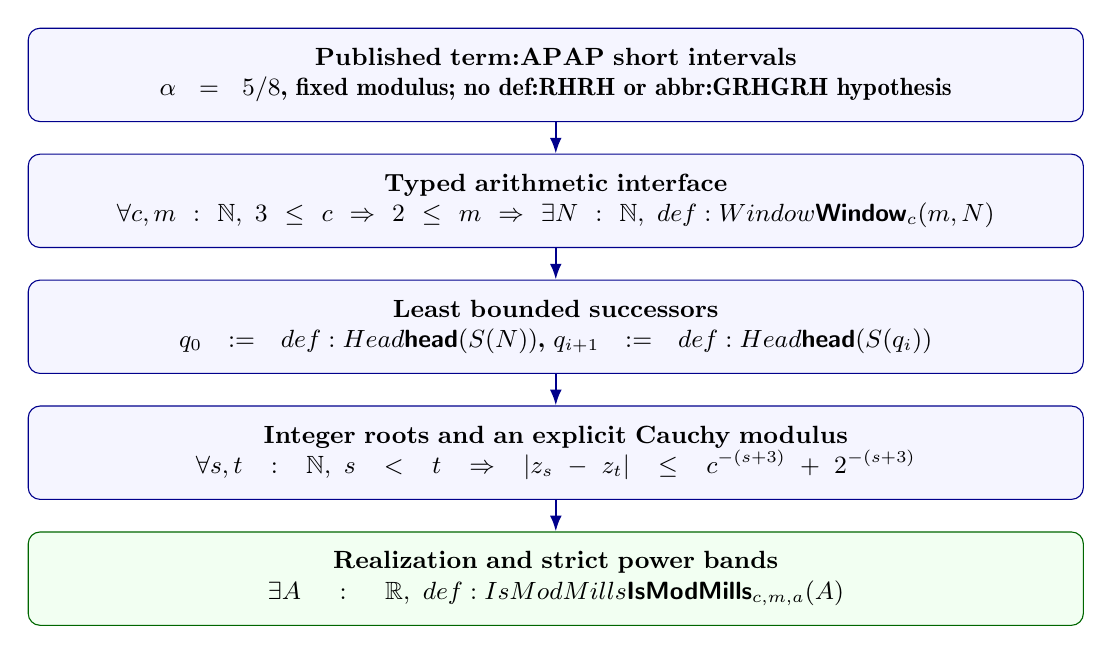
\begin{tikzpicture}[
 node distance=4mm,
 dep/.style={draw=blue!55!black,fill=blue!4,rounded corners=1.5mm,
 text width=12.9cm,align=center,font=\small,inner sep=2.5mm},
 done/.style={dep,draw=green!40!black,fill=green!5},
 flow/.style={-{Latex[length=2mm]},thick,blue!55!black}]
\node[dep] (ap) {\textbf{Published \hyperlink{term:AP}{AP} short intervals}\\
 $\alpha=5/8$, fixed modulus; no \hyperlink{def:RH}{RH} or \hyperlink{abbr:GRH}{GRH} hypothesis};
\node[dep,below=of ap] (win) {\textbf{Typed arithmetic interface}\\
 $\forall c,m:\N,\ 3\le c\Rightarrow2\le m\Rightarrow
 \exists N:\N,\ \hyperlink{def:Window}{\ensuremath{\textsf{Window}}}_c(m,N)$};
\node[dep,below=of win] (seq) {\textbf{Least bounded successors}\\
 $q_0:=\hyperlink{def:Head}{\ensuremath{\textsf{head}}}(S(N))$,
 $q_{i+1}:=\hyperlink{def:Head}{\ensuremath{\textsf{head}}}(S(q_i))$};
\node[dep,below=of seq] (code) {\textbf{Integer roots and an explicit Cauchy modulus}\\
 $\forall s,t:\N,\ s<t\Rightarrow
 |z_s-z_t|\le c^{-(s+3)}+2^{-(s+3)}$};
\node[done,below=of code] (result) {\textbf{Realization and strict power bands}\\
 $\exists A:\R,\ \hyperlink{def:IsModMills}{\ensuremath{\textsf{IsModMills}}}_{c,m,a}(A)$};
\draw[flow] (ap)--(win);
\draw[flow] (win)--(seq);
\draw[flow] (seq)--(code);
\draw[flow] (code)--(result);
\end{tikzpicture}
\caption{Sufficient dependency chain for the main theorem, for fixed
$\FormulaFit[\textstyle]{c\ge3}$, $\FormulaFit[\textstyle]{m\ge2}$, and $\FormulaFit[\textstyle]{\hyperlink{def:Nat.Coprime}{\ensuremath{\textsf{Nat.Coprime}}}(a,m)}$.
Arrows denote proof steps, not equivalences or necessity results.
No axiom catalogue is used as a substitute for a mathematical hypothesis.}
\label{fig:typed-main-dependencies}
\end{figure}

\subsection{Finite certificates and formalization boundary}
A finite certificate has the different quantifier pattern
\[\FormulaFit[\displaystyle]{
\begin{gathered}
\forall c,m,a,H:\N\ \forall q:\N\to\N\ \forall A,B:\Q, 
 \hyperlink{def:ModFull}{\ensuremath{\textsf{ModFull}}}_{c,m,a}(H,q;A,B)\Rightarrow 
 \forall x:\Q,\ (A\le x\wedge x\le B)\Rightarrow 
 \forall i:\N,\ i\le H
\\[4pt]
\Rightarrow 
 \hyperlink{def:PrimeClass}{\ensuremath{\textsf{PrimeClass}}}_{m,a}(q_i)\wedge q_i<x^{c^{i+1}}<q_i+1.
\end{gathered}
}\]
The bound $\FormulaFit[\textstyle]{H}$ cannot be dropped. Such a certificate verifies an existing
prefix and a rational inner cell; it proves no arbitrary-height extension.
The manuscript supplies mathematical proofs and typed Lean targets, not a
compiled global Lean development. A completed formalization must separately
implement the window theorem, bounded recursion, real-code realization,
and every imported library lemma. Typed notation alone is not kernel verification.

\paragraph{What the three evidence layers establish.}
The global existence result is a mathematical deduction from the stated
published \hyperlink{term:AP}{AP} theorem. The companion computations validate only bounded
examples and their exact arithmetic checks. The Lean listings describe
interfaces and finite proof source; no compiled global Lean theorem or
rendered TeX build is certified here. These forms of evidence must be
reported separately, even when they concern the same displayed predicates.


\subsection{An operational finitist interpretation}\label{sec:conclusion-finitist}
The finite layer supports a definite methodological position: report
integer data, terminating verification rules, and the bounds within which
the rules establish their conclusions. Under an operational finitist
reading, a real-valued assertion is assessed through such finite tests or
through a specified rule producing tests at arbitrary requested
precision. This reading avoids treating a decimal display as an inspected
completed infinity. It is compatible with studying the classical theorem
while withholding an ontological commitment to all classical real objects.
It is not, by itself, a proof that the classical continuum is inconsistent.
Historical finitism, Bishop-style constructivity, and recursive analysis
make different demands, as the sources in
\cref{sec:historical-overview,sec:computation-constructivity} explain
\cite{Zach2023,ConstructiveSEP2022,Bauer2017}.

If ``illusion'' is used to describe an operationally inaccessible
completed expansion, its meaning should remain philosophical and
representation-dependent. It must not be used as a mathematical inference
that irrationality or transcendence is contradictory. Those predicates
concern exact equality with rationals or zeros of integer polynomials,
not the number of decimal places printed. Elementary irrationality proofs
and Liouville's explicit transcendental construction show why finite
proofs and effective approximation are compatible with these predicates.
A strict finitist may instead decline some of the unbounded
quantification used in their usual formulations; that is a change of
framework, not an internal refutation of the classical assertions.

There is therefore a distinction between finite \emph{observations} and
finite \emph{specifications}. An observed rational interval cannot
classify every point within it. A program, formula, or inductive rule can
specify infinitely many finite tasks and support a proof about all of
them in an appropriate theory. The latter claim still incurs a proof
obligation: totality, the claimed error estimate, and the logical
principles used must be justified. Merely writing a finite symbol for an
object does not discharge that obligation, but neither does the absence
of a terminating expansion refute it.

\subsection{Uniform approximation and the remaining analytic obligation}\label{sec:conclusion-effectivity}
For the modular parameter, \cref{sec:threshold-effectivity} isolates the
computational boundary. A supplied valid threshold yields bounded prime
searches and a single rational approximation rule with an explicit error
bound for every precision. The classical existence proof for a threshold
therefore supports individual existence of a computable parameter for
each fixed admissible triple. This exposition does not turn that proof
into a uniform threshold-finding algorithm, provide a practicable
numerical constant for every triple, or establish computability of any
separately prescribed least modular parameter. These are distinct tasks.
A missing effective bound is a limitation of the presented derivation,
not a proof of noncomputability.

The same distinction prevents a finite verification from being promoted
to global existence. Increasing the height of a successful computation
produces more certified data, but not by itself a theorem that every
future search succeeds. The global proof has precisely that additional
analytic obligation. Conversely, once continuation and a modulus are
proved, it is misleading to describe the result as only a collection of
unrelated finite approximations. The uniform rule then has mathematical
content beyond any one run. A fully constructive reworking must audit the
analytic input and the realization step as well as the decidable
arithmetic; rewriting the quantifiers in typed notation does not complete
that audit.

\subsection{What positional notation does and does not explain}\label{sec:conclusion-positional}
Congruences make part of the finite interpretation particularly concrete.
A residue modulo a base power fixes an integer suffix, while a fractional
prefix fixes a rational interval. Both are finite constraints, but they
have different extension maps. Their shared notation does not identify
real completion with the inverse system of residues. The prescribed
congruence in the theorem applies to the prime outputs, and does not
specify a decimal suffix of \(\FormulaFit[\textstyle]{A}\) or decide its arithmetic classification.
Thorner--Zaman's discussion of prescribed digits supports this use of
congruences without collapsing the two kinds of information
\cite[Section~3.1]{ThornerZaman2024}.

Turing's representation correction also shows why a carry obstruction
should not be elevated into a contradiction in real arithmetic. A
canonical digit name can require a discontinuous boundary decision even
when rational approximations are available with a proved error. The
appropriate response is to state the representation and the uniformity
requirement, not to infer that effective arithmetic is impossible
\cite{TuringCorrection1938}. The integer-root Cauchy code used here is
chosen to avoid unnecessary exact digit decisions.

Arithmetic classification remains separate. Saito's unconditional
irrationality theorem and his later conditional transcendence theorem
concern the \emph{least ordinary cubic} Mills constant
\cite{Saito2025,Saito2026}. They are not consequences of our finite cell
checks, and their conclusions have not been proved here for arbitrary
modular parameters. In particular, the inspected 2026 result answers the
RH-conditional transcendence question affirmatively; citing an earlier
version as though that conditional question remained open would give an
outdated account. Unconditional cubic transcendence remains a separate
open problem in that source.

\subsection{Formal verification and further proof obligations}\label{sec:conclusion-obligations}
The finite source and the mathematical deduction must retain their
separate trust statements. In Lean, \texttt{noncomputable} exempts a
definition from code generation; it is not a theorem that the denoted
object is Turing-incomputable. The official manual even gives a
\texttt{noncomputable} implementation of a halving function using a
recursor unsupported by the compiler~\cite{LeanDefinitions}. Similarly,
a definition without that modifier need not have an axiom-free proof.
Compilation, \texttt{\#print axioms}, and a documented real representation
are different checks. No local Lean kernel run or TeX compilation is
claimed for this revision.

The next mathematical tasks can consequently be stated without
philosophical overreach. An effective numerical modular construction must
provide a usable valid threshold or a different proved continuation
method. A constructive development must specify its logic and real
representation and verify every imported principle against that choice.
A finitist reduction requires an actual translation and proof in the
chosen arithmetic, rather than a source-level absence of certain Lean
commands. A completed formalization must compile the finite checker and
the full post-window argument against pinned Lean and Mathlib versions,
with its remaining analytic dependency declared and audited. These tasks
would strengthen the evidence in different ways; none is replaced by
printing additional digits or by identifying finite suffixes with an
entire real number.

\section{Appendix}\label{sec:appendix}
\subsection{Tables}\label{sec:appendix-tables}

Abbreviations link to precise definitions, statements, usage passages, or bibliography entries.

% Insert immediately after subsection Tables (sec:appendix-tables).
% Uses simple continuous tabular blocks and existing hyperlink macros.
\begingroup
\small
\setlength{\tabcolsep}{5pt}


\renewcommand{\arraystretch}{1.15}
\begingroup
\SplitTableCaption{Abbreviations and shortened proof tags.}\label{tab:abbreviations}
\par\nobreak
\noindent
\begin{tabular}{|@{}p{0.22500\linewidth}|p{0.67500\linewidth}|}\hline
\textbf{Abbreviation or tag}&\textbf{Meaning}\\\hline
\multicolumn{2}{|c|}{\textbf{Number theory and mathematical principles}}\\\hline
\hypertarget{abbr:AP}{}\hyperlink{term:AP}{\textsf{AP}} & Arithmetic progression; here, a residue class $\FormulaFit[\textstyle]{r\equiv a\pmod m}$.\\\hline
\end{tabular}%
\par\setlength{\parskip}{0pt}\nointerlineskip
\noindent
\begin{tabular}{|@{}p{0.22500\linewidth}|p{0.67500\linewidth}|}\hline
\hypertarget{abbr:APShort}{}\hyperlink{def:APShort}{\ensuremath{\textsf{APShort}}} & Short-interval prime assertion in an arithmetic progression; the modulus is fixed.\\\hline
\end{tabular}%
\par\setlength{\parskip}{0pt}\nointerlineskip
\noindent
\begin{tabular}{|@{}p{0.22500\linewidth}|p{0.67500\linewidth}|}\hline
\hypertarget{abbr:CRT}{}\hyperlink{term:CRT}{\textsf{CRT}} & \hyperlink{term:CRT}{Chinese remainder theorem} (\hyperlink{def:CRTCompatible}{compatibility predicate}).\\\hline
\end{tabular}%
\par\setlength{\parskip}{0pt}\nointerlineskip
\noindent
\begin{tabular}{|@{}p{0.22500\linewidth}|p{0.67500\linewidth}|}\hline
\hypertarget{abbr:RH}{}\hyperlink{def:RH}{\ensuremath{\textsf{RH}}} & Riemann hypothesis for the Riemann zeta function.\\\hline
\end{tabular}%
\par\setlength{\parskip}{0pt}\nointerlineskip
\noindent
\begin{tabular}{|@{}p{0.22500\linewidth}|p{0.67500\linewidth}|}\hline
\hypertarget{abbr:GRH}{}\hyperlink{term:GRH}{\textsf{GRH}} & Generalized Riemann hypothesis; in the \hyperlink{term:AP}{AP} context, for Dirichlet $\FormulaFit[\textstyle]{L}$-functions. It is not assumed in the main modular theorem.\\\hline
\end{tabular}%
\par\setlength{\parskip}{0pt}\nointerlineskip
\noindent
\begin{tabular}{|@{}p{0.22500\linewidth}|p{0.67500\linewidth}|}\hline
\hypertarget{abbr:PRA}{}\hyperlink{term:PRA}{\textsf{PRA}} & Primitive recursive arithmetic.\\\hline
\end{tabular}%
\par\setlength{\parskip}{0pt}\nointerlineskip
\noindent
\begin{tabular}{|@{}p{0.22500\linewidth}|p{0.67500\linewidth}|}\hline
\hypertarget{abbr:gcd}{}\hyperlink{term:CRT}{$\FormulaFit[\textstyle]{\gcd}$} & Greatest common divisor.\\\hline
\end{tabular}%
\par\setlength{\parskip}{0pt}\nointerlineskip
\noindent
\begin{tabular}{|@{}p{0.22500\linewidth}|p{0.67500\linewidth}|}\hline
\hypertarget{abbr:lcm}{}\hyperlink{term:CRT}{$\FormulaFit[\textstyle]{\operatorname{lcm}}$} & Least common multiple.\\\hline
\end{tabular}%
\par\setlength{\parskip}{0pt}\nointerlineskip
\noindent
\begin{tabular}{|@{}p{0.22500\linewidth}|p{0.67500\linewidth}|}\hline
\hypertarget{abbr:GLB}{}\hyperlink{def:GLB}{\ensuremath{\textsf{GLB}}} & Greatest lower bound (infimum).\\\hline
\end{tabular}%
\par\setlength{\parskip}{0pt}\nointerlineskip
\noindent
\begin{tabular}{|@{}p{0.22500\linewidth}|p{0.67500\linewidth}|}\hline
\hypertarget{abbr:LUB}{}\hyperlink{def:LUB}{\ensuremath{\textsf{LUB}}} & Least upper bound (supremum).\\\hline
\end{tabular}%
\par\setlength{\parskip}{0pt}\nointerlineskip
\noindent
\begin{tabular}{|@{}p{0.22500\linewidth}|p{0.67500\linewidth}|}\hline
\hypertarget{abbr:MVT}{}\hyperlink{def:MVT}{\ensuremath{\textsf{MVT}}} & Mean value theorem.\\\hline
\end{tabular}%
\par\setlength{\parskip}{0pt}\nointerlineskip
\noindent
\begin{tabular}{|@{}p{0.22500\linewidth}|p{0.67500\linewidth}|}\hline
\hypertarget{abbr:IVT}{}\hyperlink{def:IVT}{\ensuremath{\textsf{IVT}}} & Intermediate value theorem.\\\hline
\end{tabular}%
\par\setlength{\parskip}{0pt}\nointerlineskip
\noindent
\begin{tabular}{|@{}p{0.22500\linewidth}|p{0.67500\linewidth}|}\hline
\hypertarget{abbr:MCT}{}\hyperlink{def:MCT}{\ensuremath{\textsf{MCT}}} & Monotone convergence theorem for real sequences.\\\hline
\end{tabular}%
\par\setlength{\parskip}{0pt}\nointerlineskip
\noindent
\begin{tabular}{|@{}p{0.22500\linewidth}|p{0.67500\linewidth}|}\hline
\hypertarget{abbr:CSB}{}\hyperlink{def:CSB}{\ensuremath{\textsf{CSB}}} & Cantor--Schr\"oder--Bernstein theorem.\\\hline
\end{tabular}%
\par\setlength{\parskip}{0pt}\nointerlineskip
\noindent
\begin{tabular}{|@{}p{0.22500\linewidth}|p{0.67500\linewidth}|}\hline
\hypertarget{abbr:LEM}{}\hyperlink{def:LEM}{\ensuremath{\textsf{LEM}}} & Law of excluded middle.\\\hline
\end{tabular}%
\par\setlength{\parskip}{0pt}\nointerlineskip
\noindent
\begin{tabular}{|@{}p{0.22500\linewidth}|p{0.67500\linewidth}|}\hline
\hypertarget{abbr:WO}{}\hyperlink{def:WO}{\ensuremath{\textsf{WO}}} & Well-ordering principle for the natural numbers.\\\hline
\end{tabular}%
\par\setlength{\parskip}{0pt}\nointerlineskip
\noindent
\begin{tabular}{|@{}p{0.22500\linewidth}|p{0.67500\linewidth}|}\hline
\hypertarget{abbr:PSeq}{}\hyperlink{def:PSeq}{\ensuremath{\textsf{PSeq}}} & Prime sequence: the strictly increasing, exhaustive enumeration of primes specified in the catalogue.\\\hline
\end{tabular}%
\par\setlength{\parskip}{0pt}\nointerlineskip
\noindent
\begin{tabular}{|@{}p{0.22500\linewidth}|p{0.67500\linewidth}|}\hline
\hypertarget{abbr:UV}{}\hyperlink{def:UV}{\ensuremath{\textsf{UV}}} & Paired lower and upper root-endpoint sequences $\FormulaFit[\textstyle]{u_n,v_n}$; the subscript $\FormulaFit[\textstyle]{c}$ denotes the general-exponent version.\\\hline
\end{tabular}%
\par\setlength{\parskip}{0pt}\nointerlineskip
\noindent
\begin{tabular}{|@{}p{0.22500\linewidth}|p{0.67500\linewidth}|}\hline
\multicolumn{2}{|c|}{\textbf{Shortened proof and predicate tags}}\\\hline
\hypertarget{abbr:Hyp}{}\hyperlink{def:Hyp}{\ensuremath{\textsf{Hyp}}} & Hypothesis available in the current proof scope.\\\hline
\end{tabular}%
\par\setlength{\parskip}{0pt}\nointerlineskip
\noindent
\begin{tabular}{|@{}p{0.22500\linewidth}|p{0.67500\linewidth}|}\hline
\hypertarget{abbr:Def}{}\hyperlink{def:Def}{\ensuremath{\textsf{Def}}} & Definition: introduce a typed local definition or unfold a catalogue definition.\\\hline
\end{tabular}%
\par\setlength{\parskip}{0pt}\nointerlineskip
\noindent
\begin{tabular}{|@{}p{0.22500\linewidth}|p{0.67500\linewidth}|}\hline
\hypertarget{abbr:Eq}{}\hyperlink{def:Eq}{\ensuremath{\textsf{Eq}}} & Equality substitution or transport.\\\hline
\end{tabular}%
\par\setlength{\parskip}{0pt}\nointerlineskip
\noindent
\begin{tabular}{|@{}p{0.22500\linewidth}|p{0.67500\linewidth}|}\hline
\hypertarget{abbr:I}{}\hyperlink{def:I}{\ensuremath{\textsf{I}}} & Introduction rule; a preceding logical symbol identifies the connective or quantifier.\\\hline
\end{tabular}%
\par\setlength{\parskip}{0pt}\nointerlineskip
\noindent
\begin{tabular}{|@{}p{0.22500\linewidth}|p{0.67500\linewidth}|}\hline
\hypertarget{abbr:E}{}\hyperlink{def:E}{\ensuremath{\textsf{E}}} & Elimination rule; a preceding logical symbol identifies the connective or quantifier.\\\hline
\end{tabular}%
\par\setlength{\parskip}{0pt}\nointerlineskip
\noindent
\begin{tabular}{|@{}p{0.22500\linewidth}|p{0.67500\linewidth}|}\hline
\hypertarget{abbr:Ext}{}\hyperlink{def:Ext}{\ensuremath{\textsf{Ext}}} & Externally cited mathematical fact; its subscript identifies the particular source.\\\hline
\end{tabular}%
\par\setlength{\parskip}{0pt}\nointerlineskip
\noindent
\begin{tabular}{|@{}p{0.22500\linewidth}|p{0.67500\linewidth}|}\hline
\hypertarget{abbr:Ind}{}\hyperlink{def:Ind}{\ensuremath{\textsf{Ind}}} & Induction on the natural-number index.\\\hline
\end{tabular}%
\par\setlength{\parskip}{0pt}\nointerlineskip
\noindent
\begin{tabular}{|@{}p{0.22500\linewidth}|p{0.67500\linewidth}|}\hline
\hypertarget{abbr:NatInduction}{}\hyperlink{def:NatInduction}{\ensuremath{\textsf{NatInduction}}} & Natural-number induction.\\\hline
\end{tabular}%
\par\setlength{\parskip}{0pt}\nointerlineskip
\noindent
\begin{tabular}{|@{}p{0.22500\linewidth}|p{0.67500\linewidth}|}\hline
\hypertarget{abbr:FiniteInd}{}\hyperlink{def:FiniteInd}{\ensuremath{\textsf{FiniteInd}}} & Finite or bounded induction.\\\hline
\end{tabular}%
\par\setlength{\parskip}{0pt}\nointerlineskip
\noindent
\begin{tabular}{|@{}p{0.22500\linewidth}|p{0.67500\linewidth}|}\hline
\hypertarget{abbr:IndHyp}{}\hyperlink{def:IndHyp}{\ensuremath{\textsf{IndHyp}}} & Induction hypothesis in the current scope.\\\hline
\end{tabular}%
\par\setlength{\parskip}{0pt}\nointerlineskip
\noindent
\begin{tabular}{|@{}p{0.22500\linewidth}|p{0.67500\linewidth}|}\hline
\hypertarget{abbr:Rec}{}\hyperlink{def:RecN}{\ensuremath{\textsf{Rec}}}, \hyperlink{def:Nat.rec}{\ensuremath{\textsf{Nat.rec}}} & Natural-number recursion or its recursor.\\\hline
\end{tabular}%
\par\setlength{\parskip}{0pt}\nointerlineskip
\noindent
\begin{tabular}{|@{}p{0.22500\linewidth}|p{0.67500\linewidth}|}\hline
\hypertarget{abbr:Conv}{}\hyperlink{def:Conv}{\ensuremath{\textsf{Conv}}} & Convergence of a sequence to the stated limit.\\\hline
\end{tabular}%
\par\setlength{\parskip}{0pt}\nointerlineskip
\noindent
\begin{tabular}{|@{}p{0.22500\linewidth}|p{0.67500\linewidth}|}\hline
\hypertarget{abbr:Lim}{}\hyperlink{def:Lim}{\ensuremath{\textsf{Lim}}} & Limit/convergence proof tag.\\\hline
\end{tabular}%
\par\setlength{\parskip}{0pt}\nointerlineskip
\noindent
\begin{tabular}{|@{}p{0.22500\linewidth}|p{0.67500\linewidth}|}\hline
\hypertarget{abbr:Inc}{}\hyperlink{def:Inc}{\ensuremath{\textsf{Inc}}}, \hyperlink{def:Dec}{\ensuremath{\textsf{Dec}}} & Nondecreasing and nonincreasing sequences, respectively; strictness is not implied.\\\hline
\end{tabular}%
\par\setlength{\parskip}{0pt}\nointerlineskip
\noindent
\begin{tabular}{|@{}p{0.22500\linewidth}|p{0.67500\linewidth}|}\hline
\hypertarget{abbr:Mono}{}\hyperlink{def:Mono}{\ensuremath{\textsf{Mono}}} & Monotonicity of functions on their stated domains.\\\hline
\end{tabular}%
\par\setlength{\parskip}{0pt}\nointerlineskip
\noindent
\begin{tabular}{|@{}p{0.22500\linewidth}|p{0.67500\linewidth}|}\hline
\hypertarget{abbr:Ord}{}\hyperlink{def:Ord}{\ensuremath{\textsf{Ord}}} & Order laws on the displayed carrier.\\\hline
\end{tabular}%
\par\setlength{\parskip}{0pt}\nointerlineskip
\noindent
\begin{tabular}{|@{}p{0.22500\linewidth}|p{0.67500\linewidth}|}\hline
\hypertarget{abbr:OrdField}{}\hyperlink{def:OrdField}{\ensuremath{\textsf{OrdField}}} & Ordered-field laws.\\\hline
\end{tabular}%
\par\setlength{\parskip}{0pt}\nointerlineskip
\noindent
\begin{tabular}{|@{}p{0.22500\linewidth}|p{0.67500\linewidth}|}\hline
\hypertarget{abbr:Arith}{}\hyperlink{def:Arith}{\ensuremath{\textsf{Arith}}} & Arithmetic laws with the displayed types.\\\hline
\end{tabular}%
\par\setlength{\parskip}{0pt}\nointerlineskip
\noindent
\begin{tabular}{|@{}p{0.22500\linewidth}|p{0.67500\linewidth}|}\hline
\hypertarget{abbr:Div}{}\hyperlink{def:Div}{\ensuremath{\textsf{Div}}} & Divisibility laws; not a division-with-remainder algorithm.\\\hline
\end{tabular}%
\par\setlength{\parskip}{0pt}\nointerlineskip
\noindent
\begin{tabular}{|@{}p{0.22500\linewidth}|p{0.67500\linewidth}|}\hline
\hypertarget{abbr:Abs}{}\hyperlink{def:Abs}{\ensuremath{\textsf{Abs}}} & Absolute-value and midpoint estimates.\\\hline
\end{tabular}%
\par\setlength{\parskip}{0pt}\nointerlineskip
\noindent
\begin{tabular}{|@{}p{0.22500\linewidth}|p{0.67500\linewidth}|}\hline
\hypertarget{abbr:Pow}{}\hyperlink{def:Pow}{\ensuremath{\textsf{Pow}}} & Power identities and their stated monotonicity rules.\\\hline
\end{tabular}%
\par\setlength{\parskip}{0pt}\nointerlineskip
\noindent
\begin{tabular}{|@{}p{0.22500\linewidth}|p{0.67500\linewidth}|}\hline
\hypertarget{abbr:Diff}{}\hyperlink{def:Diff}{\ensuremath{\textsf{Diff}}} & Differentiation rules.\\\hline
\end{tabular}%
\par\setlength{\parskip}{0pt}\nointerlineskip
\noindent
\begin{tabular}{|@{}p{0.22500\linewidth}|p{0.67500\linewidth}|}\hline
\hypertarget{abbr:Inv}{}\hyperlink{def:Inv}{\ensuremath{\textsf{Inv}}} & Inverse-function identities and order transport.\\\hline
\end{tabular}%
\par\setlength{\parskip}{0pt}\nointerlineskip
\noindent
\begin{tabular}{|@{}p{0.22500\linewidth}|p{0.67500\linewidth}|}\hline
\hypertarget{abbr:Sup}{}\hyperlink{def:Sup}{\ensuremath{\textsf{Sup}}}, \hyperlink{def:Min}{\ensuremath{\textsf{Min}}} & Supremum and least-element proof tags, respectively.\\\hline
\end{tabular}%
\par\setlength{\parskip}{0pt}\nointerlineskip
\noindent
\begin{tabular}{|@{}p{0.22500\linewidth}|p{0.67500\linewidth}|}\hline
\hypertarget{abbr:Cl}{}\hyperlink{def:Cl}{\ensuremath{\textsf{Cl}}} & Closure of a real set.\\\hline
\end{tabular}%
\par\setlength{\parskip}{0pt}\nointerlineskip
\noindent
\begin{tabular}{|@{}p{0.22500\linewidth}|p{0.67500\linewidth}|}\hline
\hypertarget{abbr:Int}{}\hyperlink{def:Int}{\ensuremath{\textsf{Int}}} & Interior of a real set; distinct from the Lean type \hyperlink{def:IntType}{\texttt{Int}}.\\\hline
\end{tabular}%
\par\setlength{\parskip}{0pt}\nointerlineskip
\noindent
\begin{tabular}{|@{}p{0.22500\linewidth}|p{0.67500\linewidth}|}\hline
\hypertarget{abbr:len}{}\hyperlink{def:len}{\ensuremath{\textsf{len}}} & Length of an interval.\\\hline
\end{tabular}%
\par\setlength{\parskip}{0pt}\nointerlineskip
\noindent
\begin{tabular}{|@{}p{0.22500\linewidth}|p{0.67500\linewidth}|}\hline
\hypertarget{abbr:FV}{}\hyperlink{def:ProofAnnotations}{$\FormulaFit[\textstyle]{\operatorname{FV}}$} & Free variables of a formula, term, or proof context.\\\hline
\end{tabular}%
\par\setlength{\parskip}{0pt}\nointerlineskip
\noindent
\begin{tabular}{|@{}p{0.22500\linewidth}|p{0.67500\linewidth}|}\hline
\hypertarget{abbr:L-blocks}{}\hyperlink{proof:L-E}{$\FormulaFit[\textstyle]{\textsf{L}_{\ast}}$} & Auxiliary lemma proof block; the subscript identifies the lemma.\\\hline
\end{tabular}%
\par\setlength{\parskip}{0pt}\nointerlineskip
\noindent
\begin{tabular}{|@{}p{0.22500\linewidth}|p{0.67500\linewidth}|}\hline
\hypertarget{abbr:R-blocks}{}\hyperlink{proof:R-1a}{$\FormulaFit[\textstyle]{\textsf{R}_{\ast}}$} & Classical route proof block.\\\hline
\end{tabular}%
\par\setlength{\parskip}{0pt}\nointerlineskip
\noindent
\begin{tabular}{|@{}p{0.22500\linewidth}|p{0.67500\linewidth}|}\hline
\hypertarget{abbr:F-blocks}{}\hyperlink{proof:F-1}{$\FormulaFit[\textstyle]{\textsf{F}_{\ast}}$} & Finite-route proof block; $\FormulaFit[\textstyle]{\hyperlink{proof:F-S}{\textsf{F}_{S}}}$ is the finite-stability supplement.\\\hline
\end{tabular}%
\par\setlength{\parskip}{0pt}\nointerlineskip
\noindent
\begin{tabular}{|@{}p{0.22500\linewidth}|p{0.67500\linewidth}|}\hline
\hypertarget{abbr:M-blocks}{}\hyperlink{proof:M-1}{$\FormulaFit[\textstyle]{\textsf{M}_{\ast}}$} & Modular (prescribed-congruence) proof block.\\\hline
\end{tabular}%
\par\setlength{\parskip}{0pt}\nointerlineskip
\noindent
\begin{tabular}{|@{}p{0.22500\linewidth}|p{0.67500\linewidth}|}\hline
\hypertarget{abbr:C-blocks}{}\hyperlink{proof:C-rat}{$\FormulaFit[\textstyle]{\textsf{C}_{\ast}}$} & Certificate or corollary proof block, including rational-enclosure and real-root interpretations.\\\hline
\end{tabular}%
\par\setlength{\parskip}{0pt}\nointerlineskip
\noindent
\begin{tabular}{|@{}p{0.22500\linewidth}|p{0.67500\linewidth}|}\hline
\hypertarget{abbr:L-QR}{}\proofref{L-QR}{\ensuremath{\textsf{L}_{QR}}} & Tag of the general root-sequence squeeze/limit lemma. Here $\FormulaFit[\textstyle]{\hyperlink{proof:L-QR}{QR}}$ is a proof identifier, not a quadratic-residue assumption.\\\hline
\end{tabular}%
\par\setlength{\parskip}{0pt}\nointerlineskip
\noindent
\begin{tabular}{|@{}p{0.22500\linewidth}|p{0.67500\linewidth}|}\hline
\multicolumn{2}{|c|}{\textbf{Type and implementation abbreviations}}\\\hline
\hypertarget{abbr:Prop}{}\hyperlink{def:Prop}{\ensuremath{\textsf{Prop}}} & Proposition sort.\\\hline
\end{tabular}%
\par\setlength{\parskip}{0pt}\nointerlineskip
\noindent
\begin{tabular}{|@{}p{0.22500\linewidth}|p{0.67500\linewidth}|}\hline
\hypertarget{abbr:Universe}{}\hyperlink{def:Universe}{\ensuremath{\textsf{Type}}} & Type universe; its level is written as a subscript when needed.\\\hline
\end{tabular}%
\par\setlength{\parskip}{0pt}\nointerlineskip
\noindent
\begin{tabular}{|@{}p{0.22500\linewidth}|p{0.67500\linewidth}|}\hline
\hypertarget{abbr:Fin}{}\hyperlink{def:Fin}{\ensuremath{\textsf{Fin}}} & Finite index type $\FormulaFit[\textstyle]{\{i:\mathbb N:i<n\}}$.\\\hline
\end{tabular}%
\par\setlength{\parskip}{0pt}\nointerlineskip
\noindent
\begin{tabular}{|@{}p{0.22500\linewidth}|p{0.67500\linewidth}|}\hline
\hypertarget{abbr:LeanNumberTypes}{}\hyperlink{def:Nat}{\texttt{Nat}}, \hyperlink{def:IntType}{\texttt{Int}} & Lean types of natural numbers and integers, respectively.\\\hline
\end{tabular}%
\par\setlength{\parskip}{0pt}\nointerlineskip
\noindent
\begin{tabular}{|@{}p{0.22500\linewidth}|p{0.67500\linewidth}|}\hline
\hypertarget{abbr:CLI}{}\hyperlink{term:CLI}{\textsf{CLI}} & Command-line interface.\\\hline
\end{tabular}%
\par\setlength{\parskip}{0pt}\nointerlineskip
\noindent
\begin{tabular}{|@{}p{0.22500\linewidth}|p{0.67500\linewidth}|}\hline
\hypertarget{abbr:JSON}{}\hyperlink{term:JSON}{\textsf{JSON}} & JavaScript Object Notation; the structured certificate-data format.\\\hline
\end{tabular}%
\par\setlength{\parskip}{0pt}\nointerlineskip
\noindent
\begin{tabular}{|@{}p{0.22500\linewidth}|p{0.67500\linewidth}|}\hline
\hypertarget{abbr:CSV}{}\hyperlink{term:CSV}{\textsf{CSV}} & Comma-separated values; the tabular data-file format.\\\hline
\end{tabular}%
\par\setlength{\parskip}{0pt}\nointerlineskip
\noindent
\begin{tabular}{|@{}p{0.22500\linewidth}|p{0.67500\linewidth}|}\hline
\hypertarget{abbr:DAG}{}\hyperlink{abbr-source:MathlibGraph}{\textsf{DAG}} & Directed acyclic graph; used for the cited declaration-dependency data.\\\hline
\end{tabular}%
\par\setlength{\parskip}{0pt}\nointerlineskip
\noindent
\begin{tabular}{|@{}p{0.22500\linewidth}|p{0.67500\linewidth}|}\hline
\multicolumn{2}{|c|}{\textbf{Bibliographic initialisms}}\\\hline
\hypertarget{abbr:LNCS}{}\hyperlink{abbr-source:OConnor2008}{\textsf{LNCS}} & Lecture Notes in Computer Science.\\\hline
\end{tabular}%
\par\setlength{\parskip}{0pt}\nointerlineskip
\noindent
\begin{tabular}{|@{}p{0.22500\linewidth}|p{0.67500\linewidth}|}\hline
\hypertarget{abbr:LEUS}{}\hyperlink{abbr-source:Tait2012}{\textsf{LEUS}} & Logic, Epistemology, and the Unity of Science.\\\hline
\end{tabular}%
\par\setlength{\parskip}{0pt}\nointerlineskip
\noindent
\begin{tabular}{|@{}p{0.22500\linewidth}|p{0.67500\linewidth}|}\hline
\hypertarget{abbr:SIAM}{}\hyperlink{abbr-source:Pratt1975}{\textsf{SIAM}} & Society for Industrial and Applied Mathematics.\\\hline
\end{tabular}%
\par\setlength{\parskip}{0pt}\nointerlineskip
\noindent
\begin{tabular}{|@{}p{0.22500\linewidth}|p{0.67500\linewidth}|}\hline
\hypertarget{abbr:TPHOLs}{}\hyperlink{abbr-source:OConnor2008}{\textsf{TPHOLs}} & Theorem Proving in Higher Order Logics.\\\hline
\end{tabular}%
\par\setlength{\parskip}{0pt}\nointerlineskip
\noindent
\begin{tabular}{|@{}p{0.22500\linewidth}|p{0.67500\linewidth}|}\hline
\hypertarget{abbr:NeurIPS}{}\hyperlink{abbr-source:MathlibGraph}{\textsf{NeurIPS}} & Neural Information Processing Systems.\\\hline
\end{tabular}%
\par\setlength{\parskip}{0pt}\nointerlineskip
\noindent
\begin{tabular}{|@{}p{0.22500\linewidth}|p{0.67500\linewidth}|}\hline
\hypertarget{abbr:N.S.}{}\hyperlink{abbr-source:Srinivasan1961}{\textsf{N.S.}} & New series, in a bibliographic volume designation.\\\hline
\end{tabular}%
\par\setlength{\parskip}{0pt}\nointerlineskip
\noindent
\begin{tabular}{|@{}p{0.22500\linewidth}|p{0.67500\linewidth}|}\hline
\multicolumn{2}{|c|}{\textbf{Shortened journal titles in the bibliography}}\\\hline
\hypertarget{abbr:journal-Acta-Arith}{}\hyperlink{abbr-source:Haneke1962}{\emph{Acta Arith.}} & Acta Arithmetica.\\\hline
\end{tabular}%
\par\setlength{\parskip}{0pt}\nointerlineskip
\noindent
\begin{tabular}{|@{}p{0.22500\linewidth}|p{0.67500\linewidth}|}\hline
\hypertarget{abbr:journal-Amer-Math-Monthly}{}\hyperlink{abbr-source:Wright1951}{\emph{Amer. Math. Monthly}} & The American Mathematical Monthly.\\\hline
\end{tabular}%
\par\setlength{\parskip}{0pt}\nointerlineskip
\noindent
\begin{tabular}{|@{}p{0.22500\linewidth}|p{0.67500\linewidth}|}\hline
\hypertarget{abbr:journal-Bull-Amer-Math-Soc}{}\hyperlink{abbr-source:Mills1947}{\emph{Bull. Amer. Math. Soc.}} & Bulletin of the American Mathematical Society.\\\hline
\end{tabular}%
\par\setlength{\parskip}{0pt}\nointerlineskip
\noindent
\begin{tabular}{|@{}p{0.22500\linewidth}|p{0.67500\linewidth}|}\hline
\hypertarget{abbr:journal-C-R-Acad-Sci-Paris}{}\hyperlink{abbr-source:Sierpinski1952}{\emph{C. R. Acad. Sci. Paris}} & Comptes rendus de l'Acad\'emie des sciences (Paris).\\\hline
\end{tabular}%
\par\setlength{\parskip}{0pt}\nointerlineskip
\noindent
\begin{tabular}{|@{}p{0.22500\linewidth}|p{0.67500\linewidth}|}\hline
\hypertarget{abbr:journal-Illinois-J-Math}{}\hyperlink{abbr-source:BennettMartinOBryantRechnitzer2018}{\emph{Illinois J. Math.}} & Illinois Journal of Mathematics.\\\hline
\end{tabular}%
\par\setlength{\parskip}{0pt}\nointerlineskip
\noindent
\begin{tabular}{|@{}p{0.22500\linewidth}|p{0.67500\linewidth}|}\hline
\hypertarget{abbr:journal-Indag-Math}{}\hyperlink{abbr-source:Kuipers1950}{\emph{Indag. Math.}} & Indagationes Mathematicae.\\\hline
\end{tabular}%
\par\setlength{\parskip}{0pt}\nointerlineskip
\noindent
\begin{tabular}{|@{}p{0.22500\linewidth}|p{0.67500\linewidth}|}\hline
\hypertarget{abbr:journal-J-Indian-Math-Soc}{}\hyperlink{abbr-source:Srinivasan1961}{\emph{J. Indian Math. Soc.}} & Journal of the Indian Mathematical Society.\\\hline
\end{tabular}%
\par\setlength{\parskip}{0pt}\nointerlineskip
\noindent
\begin{tabular}{|@{}p{0.22500\linewidth}|p{0.67500\linewidth}|}\hline
\hypertarget{abbr:journal-J-Integer-Seq}{}\hyperlink{abbr-source:CaldwellCheng2005}{\emph{J. Integer Seq.}} & Journal of Integer Sequences.\\\hline
\end{tabular}%
\par\setlength{\parskip}{0pt}\nointerlineskip
\noindent
\begin{tabular}{|@{}p{0.22500\linewidth}|p{0.67500\linewidth}|}\hline
\hypertarget{abbr:journal-J-Logic-Comput}{}\hyperlink{abbr-source:Leivant2021}{\emph{J. Logic Comput.}} & Journal of Logic and Computation.\\\hline
\end{tabular}%
\par\setlength{\parskip}{0pt}\nointerlineskip
\noindent
\begin{tabular}{|@{}p{0.22500\linewidth}|p{0.67500\linewidth}|}\hline
\hypertarget{abbr:journal-J-London-Math-Soc}{}\hyperlink{abbr-source:Wright1954}{\emph{J. London Math. Soc.}} & Journal of the London Mathematical Society.\\\hline
\end{tabular}%
\par\setlength{\parskip}{0pt}\nointerlineskip
\noindent
\begin{tabular}{|@{}p{0.22500\linewidth}|p{0.67500\linewidth}|}\hline
\hypertarget{abbr:journal-J-Number-Theory}{}\hyperlink{abbr-source:CullyHugill2023}{\emph{J. Number Theory}} & Journal of Number Theory.\\\hline
\end{tabular}%
\par\setlength{\parskip}{0pt}\nointerlineskip
\noindent
\begin{tabular}{|@{}p{0.22500\linewidth}|p{0.67500\linewidth}|}\hline
\hypertarget{abbr:journal-J-Philosophy}{}\hyperlink{abbr-source:Tait1981}{\emph{J. Philosophy}} & The Journal of Philosophy.\\\hline
\end{tabular}%
\par\setlength{\parskip}{0pt}\nointerlineskip
\noindent
\begin{tabular}{|@{}p{0.22500\linewidth}|p{0.67500\linewidth}|}\hline
\hypertarget{abbr:journal-Math-Gaz}{}\hyperlink{abbr-source:Willans1964}{\emph{Math. Gaz.}} & The Mathematical Gazette.\\\hline
\end{tabular}%
\par\setlength{\parskip}{0pt}\nointerlineskip
\noindent
\begin{tabular}{|@{}p{0.22500\linewidth}|p{0.67500\linewidth}|}\hline
\hypertarget{abbr:journal-Math-Z}{}\hyperlink{abbr-source:ThornerZaman2024}{\emph{Math. Z.}} & Mathematische Zeitschrift.\\\hline
\end{tabular}%
\par\setlength{\parskip}{0pt}\nointerlineskip
\noindent
\begin{tabular}{|@{}p{0.22500\linewidth}|p{0.67500\linewidth}|}\hline
\hypertarget{abbr:journal-Nordisk-Mat-Tidskr}{}\hyperlink{abbr-source:Bang1952}{\emph{Nordisk Mat. Tidskr.}} & Nordisk Matematisk Tidskrift.\\\hline
\end{tabular}%
\par\setlength{\parskip}{0pt}\nointerlineskip
\noindent
\begin{tabular}{|@{}p{0.22500\linewidth}|p{0.67500\linewidth}|}\hline
\hypertarget{abbr:journal-Norske-Vid-Selsk-Forh-Trondheim}{}\hyperlink{abbr-source:Srinivasan1962}{\emph{Norske Vid. Selsk. Forh. Trondheim}} & Det Kongelige Norske Videnskabers Selskab, Forhandlinger (Trondheim).\\\hline
\end{tabular}%
\par\setlength{\parskip}{0pt}\nointerlineskip
\noindent
\begin{tabular}{|@{}p{0.22500\linewidth}|p{0.67500\linewidth}|}\hline
\hypertarget{abbr:journal-Proc-Amer-Math-Soc}{}\hyperlink{abbr-source:Ore1952}{\emph{Proc. Amer. Math. Soc.}} & Proceedings of the American Mathematical Society.\\\hline
\end{tabular}%
\par\setlength{\parskip}{0pt}\nointerlineskip
\noindent
\begin{tabular}{|@{}p{0.22500\linewidth}|p{0.67500\linewidth}|}\hline
\hypertarget{abbr:journal-Quart-J-Math-Oxford-Ser}{}\hyperlink{abbr-source:Ingham1937}{\emph{Quart. J. Math. Oxford Ser.}} & The Quarterly Journal of Mathematics, Oxford Series.\\\hline
\end{tabular}%
\par\setlength{\parskip}{0pt}\nointerlineskip
\noindent
\begin{tabular}{|@{}p{0.22500\linewidth}|p{0.67500\linewidth}|}\hline
\hypertarget{abbr:journal-SIAM-J-Comput}{}\hyperlink{abbr-source:Pratt1975}{\emph{SIAM J. Comput.}} & \hyperlink{abbr:SIAM}{SIAM} Journal on Computing.\\\hline
\end{tabular}%
\par\setlength{\parskip}{0pt}\nointerlineskip
\noindent
\begin{tabular}{|@{}p{0.22500\linewidth}|p{0.67500\linewidth}|}\hline
\hypertarget{abbr:journal-Trans-Amer-Math-Soc}{}\hyperlink{abbr-source:AvigadGerhardyTowsner2010}{\emph{Trans. Amer. Math. Soc.}} & Transactions of the American Mathematical Society.\\\hline
\end{tabular}\par
\endgroup

\endgroup

% Each numerical dataset is tabulated once; exact certificates are retained separately.
{\scriptsize

\begingroup
\SplitTableCaption{Summary of the ten routes and their assertions.}\label{tab:routes}\label{tab:routes-compact}
\par\nobreak
\noindent
\begin{tabular}{|@{}p{0.05844\linewidth}|p{0.40909\linewidth}|p{0.14026\linewidth}|p{0.29221\linewidth}|}\hline
{Route} & {Presentation} & {Year} & {Assertion}\\
\hline
{1} & {Mills} & {1947} & {\cref{asser:mills}}\\
\hline
\end{tabular}%
\par\setlength{\parskip}{0pt}\nointerlineskip
\noindent
\begin{tabular}{|@{}p{0.05844\linewidth}|p{0.40909\linewidth}|p{0.14026\linewidth}|p{0.29221\linewidth}|}\hline
{2} & {Kuipers} & {1950} & {\cref{asser:kuipers}}\\
\hline
\end{tabular}%
\par\setlength{\parskip}{0pt}\nointerlineskip
\noindent
\begin{tabular}{|@{}p{0.05844\linewidth}|p{0.40909\linewidth}|p{0.14026\linewidth}|p{0.29221\linewidth}|}\hline
{3} & {Ansari-type range} & {1951} & {\cref{asser:ansari}}\\
\hline
\end{tabular}%
\par\setlength{\parskip}{0pt}\nointerlineskip
\noindent
\begin{tabular}{|@{}p{0.05844\linewidth}|p{0.40909\linewidth}|p{0.14026\linewidth}|p{0.29221\linewidth}|}\hline
{4} & {Wright} & {1951} & {\cref{asser:wright}}\\
\hline
\end{tabular}%
\par\setlength{\parskip}{0pt}\nointerlineskip
\noindent
\begin{tabular}{|@{}p{0.05844\linewidth}|p{0.40909\linewidth}|p{0.14026\linewidth}|p{0.29221\linewidth}|}\hline
{5} & {Ore-type selection} & {1952} & {\cref{asser:ore}}\\
\hline
\end{tabular}%
\par\setlength{\parskip}{0pt}\nointerlineskip
\noindent
\begin{tabular}{|@{}p{0.05844\linewidth}|p{0.40909\linewidth}|p{0.14026\linewidth}|p{0.29221\linewidth}|}\hline
{6} & {Polynomial gap} & {---} & {\cref{asser:direct}}\\
\hline
\end{tabular}%
\par\setlength{\parskip}{0pt}\nointerlineskip
\noindent
\begin{tabular}{|@{}p{0.05844\linewidth}|p{0.40909\linewidth}|p{0.14026\linewidth}|p{0.29221\linewidth}|}\hline
{7} & {Niven, fixed base} & {1951} & {\cref{asser:niven}}\\
\hline
\end{tabular}%
\par\setlength{\parskip}{0pt}\nointerlineskip
\noindent
\begin{tabular}{|@{}p{0.05844\linewidth}|p{0.40909\linewidth}|p{0.14026\linewidth}|p{0.29221\linewidth}|}\hline
{8} & {Wright-type compact sets} & {1954} & {\cref{asser:wright-metrical}}\\
\hline
\end{tabular}%
\par\setlength{\parskip}{0pt}\nointerlineskip
\noindent
\begin{tabular}{|@{}p{0.05844\linewidth}|p{0.40909\linewidth}|p{0.14026\linewidth}|p{0.29221\linewidth}|}\hline
{9} & {Lean-style interface statements} & {---} & {\cref{asser:lean-exists}}\\
\hline
\end{tabular}%
\par\setlength{\parskip}{0pt}\nointerlineskip
\noindent
\begin{tabular}{|@{}p{0.05844\linewidth}|p{0.40909\linewidth}|p{0.14026\linewidth}|p{0.29221\linewidth}|}\hline
{10} & {Prime-recurrence limit} & {---} & {\cref{asser:lean-detailed}}\\
\hline
\end{tabular}\par
\endgroup



\[\FormulaFit[\displaystyle]{
\begin{gathered}
\hyperlink{def:Ingham}{\ensuremath{\textsf{Ingham}}}\Rightarrow\exists A:\R_{>1},\ \hyperlink{def:IsMills}{\ensuremath{\textsf{IsMills}}}(A),
\\[4pt]
\hyperlink{def:Ingham}{\ensuremath{\textsf{Ingham}}}\Rightarrow\forall c:\R_{>8/3}\ \exists A:\R_{>1},\ \hyperlink{def:PrimeRep}{\ensuremath{\textsf{PrimeRep}}}(c,A),
\\[4pt]
\hyperlink{def:Bertrand}{\ensuremath{\textsf{Bertrand}}}\Rightarrow\exists A:\R_{>1},\ \hyperlink{def:IsWright}{\ensuremath{\textsf{IsWright}}}(A),
\\[4pt]
\hyperlink{def:Ingham}{\ensuremath{\textsf{Ingham}}}\Rightarrow\forall b:\R_{>1}\ \exists A:\R_{>1},\ \hyperlink{def:IsNiven}{\ensuremath{\textsf{IsNiven}}}(b,A).
\end{gathered}
}\]
The typed contracts are collected in \cref{tab:formal-predicates}.
These implications describe mathematical proofs, not compiler output.

\begingroup
\SplitTableCaption{$\FormulaFit[\textstyle]{\textsf{Pos}}$}\label{tab:postulates}
\par\nobreak
\noindent
\begin{tabular}{|@{}p{0.24545\linewidth}|p{0.65455\linewidth}|}\hline
	{$\FormulaFit[\textstyle]{\textsf{Pred}}$} & {$\FormulaFit[\textstyle]{\textsf{Formula}}$}\\
	\hline
	{\(\FormulaFit[\textstyle]{\textsf{P}_1}\)} & {\(\FormulaFit[\textstyle]{\hyperlink{def:PolyGap}{\ensuremath{\textsf{PolyGap}}}(\alpha\comma k)\Rightarrow\forall x:\R_{\ge2}\ \exists r:\N\comma \ \hyperlink{def:Prime}{\ensuremath{\textsf{Prime}}}(r)\wedge x<r\le x+kx^\alpha}\)}\\
	\hline
\end{tabular}%
\par\setlength{\parskip}{0pt}\nointerlineskip
\noindent
\begin{tabular}{|@{}p{0.24545\linewidth}|p{0.65455\linewidth}|}\hline
	{\(\FormulaFit[\textstyle]{\textsf{P}_2}\)} & {\(\FormulaFit[\textstyle]{

\hyperlink{def:PolyGap}{\ensuremath{\textsf{PolyGap}}}(\alpha\comma k)\wedge c>(1-\alpha)^{-1}
\quad 
{}\Rightarrow\exists N_0:\N_{\ge2}\ \forall N:\N_{\ge N_0}\ \exists r:\N\comma \ \hyperlink{def:Prime}{\ensuremath{\textsf{Prime}}}(r)\wedge N^c<r<(N+1)^c-1

}\)}\\
	\hline
\end{tabular}%
\par\setlength{\parskip}{0pt}\nointerlineskip
\noindent
\begin{tabular}{|@{}p{0.24545\linewidth}|p{0.65455\linewidth}|}\hline
	{\(\FormulaFit[\textstyle]{\textsf{P}_3}\)} & {\(\FormulaFit[\textstyle]{\hyperlink{def:MillsRecGeneral}{\ensuremath{\textsf{MillsRec}}}_c(q)\wedge\hyperlink{def:UVGeneral}{\ensuremath{\textsf{UV}}}_c(q\comma u\comma v)\Rightarrow\exists L:\R\comma \ \hyperlink{def:MillsSqueezeAt}{\ensuremath{\textsf{MillsSqueezeAt}}}_c(q\comma u\comma v\comma L)}\)}\\
	\hline
\end{tabular}%
\par\setlength{\parskip}{0pt}\nointerlineskip
\noindent
\begin{tabular}{|@{}p{0.24545\linewidth}|p{0.65455\linewidth}|}\hline
	{\(\FormulaFit[\textstyle]{\textsf{P}_4}\)} & {\(\FormulaFit[\textstyle]{

\hyperlink{def:PolyGap}{\ensuremath{\textsf{PolyGap}}}(\alpha\comma k)\Rightarrow\exists X_0:\R_{\ge3}\ \forall x:\R_{\ge X_0}\ \exists r:\N\comma s\comma
\quad 
\hyperlink{def:Prime}{\ensuremath{\textsf{Prime}}}(r)\wedge\hyperlink{def:Prime}{\ensuremath{\textsf{Prime}}}(s)\wedge x<r<r+1<s<x+k(1+2^\alpha)x^\alpha

}\)}\\
	\hline
\end{tabular}%
\par\setlength{\parskip}{0pt}\nointerlineskip
\noindent
\begin{tabular}{|@{}p{0.24545\linewidth}|p{0.65455\linewidth}|}\hline
	{\(\FormulaFit[\textstyle]{\textsf{P}_5}\)} & {\(\FormulaFit[\textstyle]{\hyperlink{def:BinaryTree}{\ensuremath{\textsf{Tree}}}(J)\wedge\hyperlink{def:Conv}{\ensuremath{\textsf{Conv}}}((\mu(F_m(J)))_m\comma 0)\Rightarrow\hyperlink{def:Good}{\ensuremath{\textsf{Good}}}(\Sigma(J))}\)}\\
	\hline
\end{tabular}%
\par\setlength{\parskip}{0pt}\nointerlineskip
\noindent
\begin{tabular}{|@{}p{0.24545\linewidth}|p{0.65455\linewidth}|}\hline
	{\(\FormulaFit[\textstyle]{\textsf{P}_6}\)} & {\(\FormulaFit[\textstyle]{

[K\ge2\wedge\hyperlink{def:TailPrefix}{\ensuremath{\textsf{TailPrefix}}}(q\comma m\comma K)]\Rightarrow\exists\widetilde q:\Np\to\N\ \exists L:\R\ \exists u,v:\Np\to\R\comma
\quad 
(\forall j:\{1\comma\ldots\comma m\}\comma \ \widetilde q_j=q_j)\wedge\hyperlink{def:PrimeValued}{\ensuremath{\textsf{PrimeValued}}}(\widetilde q)\wedge\hyperlink{def:MillsSqueezeAt}{\ensuremath{\textsf{MillsSqueezeAt}}}_3(\widetilde q\comma u\comma v\comma L)

}\)}\\
	\hline
\end{tabular}%
\par\setlength{\parskip}{0pt}\nointerlineskip
\noindent
\begin{tabular}{|@{}p{0.24545\linewidth}|p{0.65455\linewidth}|}\hline
	{\(\FormulaFit[\textstyle]{\hyperlink{def:Status}{\ensuremath{\textsf{Status}}}}\)} & {\(\FormulaFit[\textstyle]{\textsf{P}_1,\ldots,\textsf{P}_6:\hyperlink{def:Prop}{\ensuremath{\textsf{Prop}}};\text{proved under their displayed hypotheses}}\)}\\
	\hline
\end{tabular}\par
\endgroup


\begingroup
\SplitTableCaption{$\FormulaFit[\textstyle]{\textsf{Thm}}$}\label{tab:theorems}
\par\nobreak
\noindent
\begin{tabular}{|@{}p{0.11688\linewidth}|p{0.78312\linewidth}|}\hline
	{$\FormulaFit[\textstyle]{\textsf{Pred}}$} & {$\FormulaFit[\textstyle]{\textsf{Formula}}$}\\
	\hline
	{\(\FormulaFit[\textstyle]{\proofref{R-1a}{\textsf{R}_{1a}}}\)} & {\(\FormulaFit[\textstyle]{\hyperlink{def:Ingham}{\ensuremath{\textsf{Ingham}}}\Rightarrow\exists A:\R_{>1}\comma \ \hyperlink{def:IsMills}{\ensuremath{\textsf{IsMills}}}(A)}\)}\\
	\hline
\end{tabular}%
\par\setlength{\parskip}{0pt}\nointerlineskip
\noindent
\begin{tabular}{|@{}p{0.11688\linewidth}|p{0.78312\linewidth}|}\hline
	{\(\FormulaFit[\textstyle]{\proofref{R-1b}{\textsf{R}_{1b}}}\)} & {\(\FormulaFit[\textstyle]{\hyperlink{def:MillsRec}{\ensuremath{\textsf{MillsRec}}}(q)\wedge\hyperlink{def:UV}{\ensuremath{\textsf{UV}}}(q\comma u\comma v)\Rightarrow\forall n:\Np\comma \ u_n<u_{n+1}<v_{n+1}<v_n}\)}\\
	\hline
\end{tabular}%
\par\setlength{\parskip}{0pt}\nointerlineskip
\noindent
\begin{tabular}{|@{}p{0.11688\linewidth}|p{0.78312\linewidth}|}\hline
	{\(\FormulaFit[\textstyle]{\proofref{R-1p}{\textsf{R}_{1p}}}\)} & {\(\FormulaFit[\textstyle]{

[K\ge2\wedge\hyperlink{def:TailPrefix}{\ensuremath{\textsf{TailPrefix}}}(q\comma m\comma K)]\Rightarrow\exists\widetilde q:\Np\to\N\ \exists A:\R\ \exists u,v:\Np\to\R\comma
\quad 
\hyperlink{def:PrimeValued}{\ensuremath{\textsf{PrimeValued}}}(\widetilde q)\wedge\hyperlink{def:MillsSqueezeAt}{\ensuremath{\textsf{MillsSqueezeAt}}}_3(\widetilde q\comma u\comma v\comma A)
\quad 
{}\wedge\ (\forall j:\{1\comma\ldots\comma m\}\comma \ \widetilde q_j=q_j)
\quad 
{}\wedge\forall n:\Np\comma \ \fl{A^{3^n}}=\iota(\widetilde q_n)\comma \quad v_n-u_n\le(q_1+1)3^{-n}

}\)}\\
	\hline
\end{tabular}%
\par\setlength{\parskip}{0pt}\nointerlineskip
\noindent
\begin{tabular}{|@{}p{0.11688\linewidth}|p{0.78312\linewidth}|}\hline
	{\(\FormulaFit[\textstyle]{\proofref{R-2}{\textsf{R}_2}}\)} & {\(\FormulaFit[\textstyle]{\hyperlink{def:Ingham}{\ensuremath{\textsf{Ingham}}}\Rightarrow\forall c:\N_{\ge3}\ \exists A:\R_{>1}\comma \ \hyperlink{def:IsKuipers}{\ensuremath{\textsf{IsKuipers}}}(c\comma A)}\)}\\
	\hline
\end{tabular}%
\par\setlength{\parskip}{0pt}\nointerlineskip
\noindent
\begin{tabular}{|@{}p{0.11688\linewidth}|p{0.78312\linewidth}|}\hline
	{\(\FormulaFit[\textstyle]{\proofref{R-3}{\textsf{R}_3}}\)} & {\(\FormulaFit[\textstyle]{\hyperlink{def:Ingham}{\ensuremath{\textsf{Ingham}}}\Rightarrow\forall c:\R_{>8/3}\ \exists A:\R_{>1}\comma \ \hyperlink{def:IsAnsari}{\ensuremath{\textsf{IsAnsari}}}(c\comma A)}\)}\\
	\hline
\end{tabular}%
\par\setlength{\parskip}{0pt}\nointerlineskip
\noindent
\begin{tabular}{|@{}p{0.11688\linewidth}|p{0.78312\linewidth}|}\hline
	{\(\FormulaFit[\textstyle]{\proofref{R-4}{\textsf{R}_4}}\)} & {\(\FormulaFit[\textstyle]{\hyperlink{def:Bertrand}{\ensuremath{\textsf{Bertrand}}}\Rightarrow\exists A:\R_{>1}\comma \ \hyperlink{def:IsWright}{\ensuremath{\textsf{IsWright}}}(A)}\)}\\
	\hline
\end{tabular}%
\par\setlength{\parskip}{0pt}\nointerlineskip
\noindent
\begin{tabular}{|@{}p{0.11688\linewidth}|p{0.78312\linewidth}|}\hline
	{\(\FormulaFit[\textstyle]{\proofref{R-5}{\textsf{R}_5}}\)} & {\(\FormulaFit[\textstyle]{

\hyperlink{def:Continuous}{\ensuremath{\textsf{Continuous}}}(f)\wedge\hyperlink{def:OreBound}{\ensuremath{\textsf{OreBound}}}(f\comma q\comma \delta\comma \epsilon)\wedge q_1-\delta_1>0
\quad 
{}\Rightarrow\exists A:\R_{>0}\ \forall n:\Np\comma \ q_n-\delta_n\le f^{[n-1]}(A)\le q_n+\epsilon_n

}\)}\\
	\hline
\end{tabular}%
\par\setlength{\parskip}{0pt}\nointerlineskip
\noindent
\begin{tabular}{|@{}p{0.11688\linewidth}|p{0.78312\linewidth}|}\hline
	{\(\FormulaFit[\textstyle]{\proofref{R-6}{\textsf{R}_6}}\)} & {\(\FormulaFit[\textstyle]{\hyperlink{def:PolyGap}{\ensuremath{\textsf{PolyGap}}}(\alpha\comma k)\wedge c>(1-\alpha)^{-1}\Rightarrow\exists A:\R_{>1}\comma \ \hyperlink{def:PrimeRep}{\ensuremath{\textsf{PrimeRep}}}(c\comma A)}\)}\\
	\hline
\end{tabular}%
\par\setlength{\parskip}{0pt}\nointerlineskip
\noindent
\begin{tabular}{|@{}p{0.11688\linewidth}|p{0.78312\linewidth}|}\hline
	{\(\FormulaFit[\textstyle]{\proofref{R-7}{\textsf{R}_7}}\)} & {\(\FormulaFit[\textstyle]{\hyperlink{def:Ingham}{\ensuremath{\textsf{Ingham}}}\Rightarrow\forall b:\R_{>1}\ \exists A:\R_{>1}\comma \ \hyperlink{def:IsNiven}{\ensuremath{\textsf{IsNiven}}}(b\comma A)}\)}\\
	\hline
\end{tabular}%
\par\setlength{\parskip}{0pt}\nointerlineskip
\noindent
\begin{tabular}{|@{}p{0.11688\linewidth}|p{0.78312\linewidth}|}\hline
	{\(\FormulaFit[\textstyle]{\proofref{R-8}{\textsf{R}_8}}\)} & {\(\FormulaFit[\textstyle]{

\hyperlink{def:Ingham}{\ensuremath{\textsf{Ingham}}}\Rightarrow\forall c:\R_{>8/3}\ \forall b:\R_{>1}\ \exists\Sigma_a,\Sigma_w,\Sigma_n:\hyperlink{def:Set}{\ensuremath{\textsf{Set}}}(\R)\comma
\quad 
\Sigma_a\subseteq\Theta_{a\comma c}\wedge\Sigma_w\subseteq\Theta_w\wedge\Sigma_n\subseteq\Theta_{n\comma b}
\quad 
{}\wedge\hyperlink{def:Good}{\ensuremath{\textsf{Good}}}(\Sigma_a)\wedge\hyperlink{def:Good}{\ensuremath{\textsf{Good}}}(\Sigma_w)\wedge\hyperlink{def:Good}{\ensuremath{\textsf{Good}}}(\Sigma_n)

}\)}\\
	\hline
\end{tabular}%
\par\setlength{\parskip}{0pt}\nointerlineskip
\noindent
\begin{tabular}{|@{}p{0.11688\linewidth}|p{0.78312\linewidth}|}\hline
	{\(\FormulaFit[\textstyle]{\proofref{R-9e}{\textsf{R}_{9e}}}\)} & {\(\FormulaFit[\textstyle]{\hyperlink{def:Ingham}{\ensuremath{\textsf{Ingham}}}\Rightarrow\exists A:\R_{>1}\comma \ \hyperlink{def:IsMills}{\ensuremath{\textsf{IsMills}}}(A)}\)}\\
	\hline
\end{tabular}%
\par\setlength{\parskip}{0pt}\nointerlineskip
\noindent
\begin{tabular}{|@{}p{0.11688\linewidth}|p{0.78312\linewidth}|}\hline
	{\(\FormulaFit[\textstyle]{\proofref{R-9m}{\textsf{R}_{9m}}}\)} & {\(\FormulaFit[\textstyle]{(\exists A:\R\comma \hyperlink{def:IsMills}{\ensuremath{\textsf{IsMills}}}(A))\Rightarrow\exists! A:\R\comma \hyperlink{def:IsMinMills}{\ensuremath{\textsf{IsMinMills}}}(A)}\)}\\
	\hline
\end{tabular}%
\par\setlength{\parskip}{0pt}\nointerlineskip
\noindent
\begin{tabular}{|@{}p{0.11688\linewidth}|p{0.78312\linewidth}|}\hline
	{\(\FormulaFit[\textstyle]{\proofref{R-9i}{\textsf{R}_{9i}}}\)} & {\(\FormulaFit[\textstyle]{\hyperlink{def:ExtSaito2025}{\ensuremath{\textsf{Ext}_{\mathtt{Saito2025}}}}\Rightarrow\forall A:\R\comma \hyperlink{def:IsMinMills}{\ensuremath{\textsf{IsMinMills}}}(A)\Rightarrow\hyperlink{def:Irrational}{\ensuremath{\textsf{Irrational}}}(A)}\)}\\
	\hline
\end{tabular}%
\par\setlength{\parskip}{0pt}\nointerlineskip
\noindent
\begin{tabular}{|@{}p{0.11688\linewidth}|p{0.78312\linewidth}|}\hline
	{\(\FormulaFit[\textstyle]{\proofref{R-9r}{\textsf{R}_{9r}}}\)} & {\(\FormulaFit[\textstyle]{

\hyperlink{def:ExtCaldwellCheng2005}{\ensuremath{\textsf{Ext}_{\mathtt{CaldwellCheng2005}}}}\wedge\hyperlink{def:RH}{\ensuremath{\textsf{RH}}}
\quad 
{}\Rightarrow\forall A:\R\comma \hyperlink{def:IsMinMills}{\ensuremath{\textsf{IsMinMills}}}(A)\Rightarrow1.3063778838<A<1.3063778839

}\)}\\
	\hline
\end{tabular}%
\par\setlength{\parskip}{0pt}\nointerlineskip
\noindent
\begin{tabular}{|@{}p{0.11688\linewidth}|p{0.78312\linewidth}|}\hline
	{\(\FormulaFit[\textstyle]{\proofref{R-10}{\textsf{R}_{10}}}\)} & {\(\FormulaFit[\textstyle]{

\hyperlink{def:PrimeValued}{\ensuremath{\textsf{PrimeValued}}}(q)\wedge\hyperlink{def:MillsRec}{\ensuremath{\textsf{MillsRec}}}(q)\Rightarrow\exists A:\R_{>1}\comma
\quad 
\hyperlink{def:IsMills}{\ensuremath{\textsf{IsMills}}}(A)\wedge\forall n:\Np\comma \ \fl{A^{3^n}}=\iota(q_n)

}\)}\\
	\hline
\end{tabular}%
\par\setlength{\parskip}{0pt}\nointerlineskip
\noindent
\begin{tabular}{|@{}p{0.11688\linewidth}|p{0.78312\linewidth}|}\hline
	{\(\FormulaFit[\textstyle]{\proofref{C-rat}{\textsf{C}_{\mathrm{rat}}}}\)} & {\(\FormulaFit[\textstyle]{

\hyperlink{def:MillsSqueezeAt}{\ensuremath{\textsf{MillsSqueezeAt}}}_3(q\comma u\comma v\comma A)\wedge\hyperlink{def:RationalCert}{\ensuremath{\textsf{RationalCert}}}(a\comma b\comma q_m\comma m)
\quad 
{}\Rightarrow a<A<b\ \wedge\ |A-(a+b)/2|<(b-a)/2

}\)}\\
	\hline
\end{tabular}\par
\endgroup


% Proofs, including the algorithmic lemmas, occur only in the main proof table.

The algorithmic predicates and computational status records are in \cref{tab:formal-predicates}.

\[\FormulaFit[\displaystyle]{
\begin{gathered}
\proofref{R-1a}{\textsf{R}_{1a}}\comma \proofref{R-2}{\textsf{R}_2}\comma \proofref{R-3}{\textsf{R}_3}\comma \proofref{R-6}{\textsf{R}_6}\ \longleftarrow\ \proofref{L-P}{\textsf{L}_P}\ \longleftarrow\ \proofref{L-G}{\textsf{L}_G}\comma
\\[4pt]
\proofref{R-4}{\textsf{R}_4}\ \longleftarrow\ \proofref{L-W}{\textsf{L}_W}\ \longleftarrow\ \hyperlink{def:Bertrand}{\ensuremath{\textsf{Bertrand}}}\comma
\\[4pt]
\proofref{R-8}{\textsf{R}_8}\ \longleftarrow\ \{\proofref{L-2P}{\textsf{L}_{2P}}\comma \proofref{L-T}{\textsf{L}_T}\comma \proofref{R-7}{\textsf{R}_7}\}\comma
\\[4pt]
\proofref{R-9i}{\textsf{R}_{9i}}\ \longleftarrow\ \hyperlink{def:ExtSaito2025}{\ensuremath{\textsf{Ext}_{\mathtt{Saito2025}}}}\comma 
\proofref{R-9r}{\textsf{R}_{9r}}\ \longleftarrow\ \{\hyperlink{def:RH}{\ensuremath{\textsf{RH}}}\comma \hyperlink{def:ExtCaldwellCheng2005}{\ensuremath{\textsf{Ext}_{\mathtt{CaldwellCheng2005}}}}\}\comma
\\[4pt]
\proofref{R-10}{\textsf{R}_{10}}\ \longleftarrow\ \proofref{L-QR}{\textsf{L}_{QR}}.
\end{gathered}
}\]

\[\FormulaFit[\displaystyle]{
(q_1\comma q_2\comma q_3\comma q_4):=(2\comma 11\comma 1361\comma 2521008887)\comma 
(u_n\comma v_n):=(q_n^{3^{-n}}\comma (q_n+1)^{3^{-n}})(1\le n\le4).
}\]


\begingroup
\scriptsize
\begingroup
\SplitTableCaption{$\FormulaFit[\textstyle]{u_n^{(c)}=q_n^{c^{-n}}\comma  v_n^{(c)}=(q_n+1)^{c^{-n}}}$ ($\FormulaFit[\textstyle]{c=3\comma 5}$). Decimal entries are rounded, not interval certificates.}\label{tab:exponent-typo}\label{tab:monotonicity}
\par\nobreak
\noindent
\begin{tabular}{|@{}p{0.03506\linewidth}|p{0.14610\linewidth}|p{0.17971\linewidth}|p{0.17971\linewidth}|p{0.17971\linewidth}|p{0.17971\linewidth}|}\hline
{$\FormulaFit[\textstyle]{n}$} & {$\FormulaFit[\textstyle]{q_n}$} & {$\FormulaFit[\textstyle]{u_n^{(3)}}$} & {$\FormulaFit[\textstyle]{v_n^{(3)}}$} & {$\FormulaFit[\textstyle]{u_n^{(5)}}$} & {$\FormulaFit[\textstyle]{v_n^{(5)}}$}\\
\hline
{$\FormulaFit[\textstyle]{1}$} & {$\FormulaFit[\textstyle]{2}$} & {$\FormulaFit[\textstyle]{1.259921049895}$} & {$\FormulaFit[\textstyle]{1.442249570307}$} & {$\FormulaFit[\textstyle]{1.148698354997}$} & {$\FormulaFit[\textstyle]{1.245730939616}$}\\
\hline
\end{tabular}%
\par\setlength{\parskip}{0pt}\nointerlineskip
\noindent
\begin{tabular}{|@{}p{0.03506\linewidth}|p{0.14610\linewidth}|p{0.17971\linewidth}|p{0.17971\linewidth}|p{0.17971\linewidth}|p{0.17971\linewidth}|}\hline
{$\FormulaFit[\textstyle]{2}$} & {$\FormulaFit[\textstyle]{11}$} & {$\FormulaFit[\textstyle]{1.305299880795}$} & {$\FormulaFit[\textstyle]{1.317980629213}$} & {$\FormulaFit[\textstyle]{1.100666395993}$} & {$\FormulaFit[\textstyle]{1.104503890181}$}\\
\hline
\end{tabular}%
\par\setlength{\parskip}{0pt}\nointerlineskip
\noindent
\begin{tabular}{|@{}p{0.03506\linewidth}|p{0.14610\linewidth}|p{0.17971\linewidth}|p{0.17971\linewidth}|p{0.17971\linewidth}|p{0.17971\linewidth}|}\hline
{$\FormulaFit[\textstyle]{3}$} & {$\FormulaFit[\textstyle]{1361}$} & {$\FormulaFit[\textstyle]{1.306377883825}$} & {$\FormulaFit[\textstyle]{1.306413421854}$} & {$\FormulaFit[\textstyle]{1.059426580566}$} & {$\FormulaFit[\textstyle]{1.059432805640}$}\\
\hline
\end{tabular}%
\par\setlength{\parskip}{0pt}\nointerlineskip
\noindent
\begin{tabular}{|@{}p{0.03506\linewidth}|p{0.14610\linewidth}|p{0.17971\linewidth}|p{0.17971\linewidth}|p{0.17971\linewidth}|p{0.17971\linewidth}|}\hline
{$\FormulaFit[\textstyle]{4}$} & {$\FormulaFit[\textstyle]{2521008887}$} & {$\FormulaFit[\textstyle]{1.306377883863}$} & {$\FormulaFit[\textstyle]{1.306377883869}$} & {$\FormulaFit[\textstyle]{1.035243515808}$} & {$\FormulaFit[\textstyle]{1.035243515808}$}\\
\hline
\end{tabular}\par
\endgroup

\[\FormulaFit[\displaystyle]{
\begin{gathered}
u_1^{(3)}<u_2^{(3)}<u_3^{(3)}<u_4^{(3)}\comma \
v_1^{(3)}>v_2^{(3)}>v_3^{(3)}>v_4^{(3)}\comma
\\[4pt]
\
u_1^{(5)}>u_2^{(5)}>u_3^{(5)}>u_4^{(5)}\comma \
v_1^{(5)}>v_2^{(5)}>v_3^{(5)}>v_4^{(5)}.
\end{gathered}
}\]
\endgroup

\begingroup
\SplitTableCaption{$\FormulaFit[\textstyle]{\hyperlink{def:CubicPrefix}{\ensuremath{\textsf{CubicPrefix}}}}$}\label{tab:cubic-prefix}
\par\nobreak
\noindent
\begin{tabular}{|@{}p{0.03506\linewidth}|p{0.18117\linewidth}|p{0.34188\linewidth}|p{0.34188\linewidth}|}\hline
	{$\FormulaFit[\textstyle]{\textsf{n}}$} & {$\FormulaFit[\textstyle]{\textsf{\ensuremath{q_n}}}$} & {$\FormulaFit[\textstyle]{\textsf{\ensuremath{a_n\le u_n}}}$} & {$\FormulaFit[\textstyle]{\textsf{\ensuremath{v_n\le b_n}}}$}\\
	\hline
	{$\FormulaFit[\textstyle]{1}$} & {$\FormulaFit[\textstyle]{2}$} & {$\FormulaFit[\textstyle]{\dfrac{1259921049894873164}{10^{18}}}$} & {$\FormulaFit[\textstyle]{\dfrac{1442249570307408383}{10^{18}}}$}\\
	\hline
\end{tabular}%
\par\setlength{\parskip}{0pt}\nointerlineskip
\noindent
\begin{tabular}{|@{}p{0.03506\linewidth}|p{0.18117\linewidth}|p{0.34188\linewidth}|p{0.34188\linewidth}|}\hline
	{$\FormulaFit[\textstyle]{2}$} & {$\FormulaFit[\textstyle]{11}$} & {$\FormulaFit[\textstyle]{\dfrac{1305299880794919784}{10^{18}}}$} & {$\FormulaFit[\textstyle]{\dfrac{1317980629213002240}{10^{18}}}$}\\
	\hline
\end{tabular}%
\par\setlength{\parskip}{0pt}\nointerlineskip
\noindent
\begin{tabular}{|@{}p{0.03506\linewidth}|p{0.18117\linewidth}|p{0.34188\linewidth}|p{0.34188\linewidth}|}\hline
	{$\FormulaFit[\textstyle]{3}$} & {$\FormulaFit[\textstyle]{1361}$} & {$\FormulaFit[\textstyle]{\dfrac{1306377883824695767}{10^{18}}}$} & {$\FormulaFit[\textstyle]{\dfrac{1306413421853598757}{10^{18}}}$}\\
	\hline
\end{tabular}%
\par\setlength{\parskip}{0pt}\nointerlineskip
\noindent
\begin{tabular}{|@{}p{0.03506\linewidth}|p{0.18117\linewidth}|p{0.34188\linewidth}|p{0.34188\linewidth}|}\hline
	{$\FormulaFit[\textstyle]{4}$} & {$\FormulaFit[\textstyle]{2521008887}$} & {$\FormulaFit[\textstyle]{\dfrac{1306377883863080690}{10^{18}}}$} & {$\FormulaFit[\textstyle]{\dfrac{1306377883869478178}{10^{18}}}$}\\
	\hline
\end{tabular}\par
\endgroup



\begin{spreadlines}{10pt}
	\[
\FormulaFit[\displaystyle]{\begin{gathered}

	\hyperlink{def:CubicPrefix}{\ensuremath{\textsf{CubicPrefix}}}((2\comma 11\comma 1361\comma 2521008887)\comma 4)\comma \\
	\forall j:\{1\comma 2\comma 3\}\comma  q_j^3<q_{j+1}<(q_j+1)^3-1\comma \\
	\left(\frac{13063778838}{10^{10}}\right)^{81}<2521008887\comma 
	2521008888<\left(\frac{13063778839}{10^{10}}\right)^{81}\comma \\
	\frac{13063778838}{10^{10}}<q_4^{1/81}<(q_4+1)^{1/81}<\frac{13063778839}{10^{10}}.
	
\end{gathered}}
\]
\end{spreadlines}


\begingroup
\SplitTableCaption{$\FormulaFit[\textstyle]{N^c<r<(N+1)^c-1\comma \hyperlink{def:Prime}{\ensuremath{\textsf{Prime}}}(r)}$. The witness is the least prime greater than $\FormulaFit[\textstyle]{N^c}$.}\label{tab:prime-intervals}
\par\nobreak
\noindent
\begin{tabular}{|@{}p{0.04675\linewidth}|p{0.05844\linewidth}|p{0.23961\linewidth}|p{0.25130\linewidth}|p{0.30390\linewidth}|}\hline
{$\FormulaFit[\textstyle]{N}$} & {$\FormulaFit[\textstyle]{c}$} & {$\FormulaFit[\textstyle]{N^c}$} & {$\FormulaFit[\textstyle]{(N+1)^c-1}$} & {$\FormulaFit[\textstyle]{r}$}\\
\hline
{$\FormulaFit[\textstyle]{2}$} & {$\FormulaFit[\textstyle]{3}$} & {$\FormulaFit[\textstyle]{8}$} & {$\FormulaFit[\textstyle]{26}$} & {$\FormulaFit[\textstyle]{11}$}\\
\hline
\end{tabular}%
\par\setlength{\parskip}{0pt}\nointerlineskip
\noindent
\begin{tabular}{|@{}p{0.04675\linewidth}|p{0.05844\linewidth}|p{0.23961\linewidth}|p{0.25130\linewidth}|p{0.30390\linewidth}|}\hline
{$\FormulaFit[\textstyle]{3}$} & {$\FormulaFit[\textstyle]{3}$} & {$\FormulaFit[\textstyle]{27}$} & {$\FormulaFit[\textstyle]{63}$} & {$\FormulaFit[\textstyle]{29}$}\\
\hline
\end{tabular}%
\par\setlength{\parskip}{0pt}\nointerlineskip
\noindent
\begin{tabular}{|@{}p{0.04675\linewidth}|p{0.05844\linewidth}|p{0.23961\linewidth}|p{0.25130\linewidth}|p{0.30390\linewidth}|}\hline
{$\FormulaFit[\textstyle]{4}$} & {$\FormulaFit[\textstyle]{3}$} & {$\FormulaFit[\textstyle]{64}$} & {$\FormulaFit[\textstyle]{124}$} & {$\FormulaFit[\textstyle]{67}$}\\
\hline
\end{tabular}%
\par\setlength{\parskip}{0pt}\nointerlineskip
\noindent
\begin{tabular}{|@{}p{0.04675\linewidth}|p{0.05844\linewidth}|p{0.23961\linewidth}|p{0.25130\linewidth}|p{0.30390\linewidth}|}\hline
{$\FormulaFit[\textstyle]{5}$} & {$\FormulaFit[\textstyle]{3}$} & {$\FormulaFit[\textstyle]{125}$} & {$\FormulaFit[\textstyle]{215}$} & {$\FormulaFit[\textstyle]{127}$}\\
\hline
\end{tabular}%
\par\setlength{\parskip}{0pt}\nointerlineskip
\noindent
\begin{tabular}{|@{}p{0.04675\linewidth}|p{0.05844\linewidth}|p{0.23961\linewidth}|p{0.25130\linewidth}|p{0.30390\linewidth}|}\hline
{$\FormulaFit[\textstyle]{6}$} & {$\FormulaFit[\textstyle]{3}$} & {$\FormulaFit[\textstyle]{216}$} & {$\FormulaFit[\textstyle]{342}$} & {$\FormulaFit[\textstyle]{223}$}\\
\hline
\end{tabular}%
\par\setlength{\parskip}{0pt}\nointerlineskip
\noindent
\begin{tabular}{|@{}p{0.04675\linewidth}|p{0.05844\linewidth}|p{0.23961\linewidth}|p{0.25130\linewidth}|p{0.30390\linewidth}|}\hline
{$\FormulaFit[\textstyle]{7}$} & {$\FormulaFit[\textstyle]{3}$} & {$\FormulaFit[\textstyle]{343}$} & {$\FormulaFit[\textstyle]{511}$} & {$\FormulaFit[\textstyle]{347}$}\\
\hline
\end{tabular}%
\par\setlength{\parskip}{0pt}\nointerlineskip
\noindent
\begin{tabular}{|@{}p{0.04675\linewidth}|p{0.05844\linewidth}|p{0.23961\linewidth}|p{0.25130\linewidth}|p{0.30390\linewidth}|}\hline
{$\FormulaFit[\textstyle]{8}$} & {$\FormulaFit[\textstyle]{3}$} & {$\FormulaFit[\textstyle]{512}$} & {$\FormulaFit[\textstyle]{728}$} & {$\FormulaFit[\textstyle]{521}$}\\
\hline
\end{tabular}%
\par\setlength{\parskip}{0pt}\nointerlineskip
\noindent
\begin{tabular}{|@{}p{0.04675\linewidth}|p{0.05844\linewidth}|p{0.23961\linewidth}|p{0.25130\linewidth}|p{0.30390\linewidth}|}\hline
{$\FormulaFit[\textstyle]{9}$} & {$\FormulaFit[\textstyle]{3}$} & {$\FormulaFit[\textstyle]{729}$} & {$\FormulaFit[\textstyle]{999}$} & {$\FormulaFit[\textstyle]{733}$}\\
\hline
\end{tabular}%
\par\setlength{\parskip}{0pt}\nointerlineskip
\noindent
\begin{tabular}{|@{}p{0.04675\linewidth}|p{0.05844\linewidth}|p{0.23961\linewidth}|p{0.25130\linewidth}|p{0.30390\linewidth}|}\hline
{$\FormulaFit[\textstyle]{10}$} & {$\FormulaFit[\textstyle]{3}$} & {$\FormulaFit[\textstyle]{1000}$} & {$\FormulaFit[\textstyle]{1330}$} & {$\FormulaFit[\textstyle]{1009}$}\\
\hline
\end{tabular}%
\par\setlength{\parskip}{0pt}\nointerlineskip
\noindent
\begin{tabular}{|@{}p{0.04675\linewidth}|p{0.05844\linewidth}|p{0.23961\linewidth}|p{0.25130\linewidth}|p{0.30390\linewidth}|}\hline
{$\FormulaFit[\textstyle]{11}$} & {$\FormulaFit[\textstyle]{3}$} & {$\FormulaFit[\textstyle]{1331}$} & {$\FormulaFit[\textstyle]{1727}$} & {$\FormulaFit[\textstyle]{1361}$}\\
\hline
\end{tabular}%
\par\setlength{\parskip}{0pt}\nointerlineskip
\noindent
\begin{tabular}{|@{}p{0.04675\linewidth}|p{0.05844\linewidth}|p{0.23961\linewidth}|p{0.25130\linewidth}|p{0.30390\linewidth}|}\hline
{$\FormulaFit[\textstyle]{12}$} & {$\FormulaFit[\textstyle]{3}$} & {$\FormulaFit[\textstyle]{1728}$} & {$\FormulaFit[\textstyle]{2196}$} & {$\FormulaFit[\textstyle]{1733}$}\\
\hline
\end{tabular}%
\par\setlength{\parskip}{0pt}\nointerlineskip
\noindent
\begin{tabular}{|@{}p{0.04675\linewidth}|p{0.05844\linewidth}|p{0.23961\linewidth}|p{0.25130\linewidth}|p{0.30390\linewidth}|}\hline
{$\FormulaFit[\textstyle]{13}$} & {$\FormulaFit[\textstyle]{3}$} & {$\FormulaFit[\textstyle]{2197}$} & {$\FormulaFit[\textstyle]{2743}$} & {$\FormulaFit[\textstyle]{2203}$}\\
\hline
\end{tabular}%
\par\setlength{\parskip}{0pt}\nointerlineskip
\noindent
\begin{tabular}{|@{}p{0.04675\linewidth}|p{0.05844\linewidth}|p{0.23961\linewidth}|p{0.25130\linewidth}|p{0.30390\linewidth}|}\hline
{$\FormulaFit[\textstyle]{14}$} & {$\FormulaFit[\textstyle]{3}$} & {$\FormulaFit[\textstyle]{2744}$} & {$\FormulaFit[\textstyle]{3374}$} & {$\FormulaFit[\textstyle]{2749}$}\\
\hline
\end{tabular}%
\par\setlength{\parskip}{0pt}\nointerlineskip
\noindent
\begin{tabular}{|@{}p{0.04675\linewidth}|p{0.05844\linewidth}|p{0.23961\linewidth}|p{0.25130\linewidth}|p{0.30390\linewidth}|}\hline
{$\FormulaFit[\textstyle]{15}$} & {$\FormulaFit[\textstyle]{3}$} & {$\FormulaFit[\textstyle]{3375}$} & {$\FormulaFit[\textstyle]{4095}$} & {$\FormulaFit[\textstyle]{3389}$}\\
\hline
\end{tabular}%
\par\setlength{\parskip}{0pt}\nointerlineskip
\noindent
\begin{tabular}{|@{}p{0.04675\linewidth}|p{0.05844\linewidth}|p{0.23961\linewidth}|p{0.25130\linewidth}|p{0.30390\linewidth}|}\hline
{$\FormulaFit[\textstyle]{16}$} & {$\FormulaFit[\textstyle]{3}$} & {$\FormulaFit[\textstyle]{4096}$} & {$\FormulaFit[\textstyle]{4912}$} & {$\FormulaFit[\textstyle]{4099}$}\\
\hline
\end{tabular}%
\par\setlength{\parskip}{0pt}\nointerlineskip
\noindent
\begin{tabular}{|@{}p{0.04675\linewidth}|p{0.05844\linewidth}|p{0.23961\linewidth}|p{0.25130\linewidth}|p{0.30390\linewidth}|}\hline
{$\FormulaFit[\textstyle]{17}$} & {$\FormulaFit[\textstyle]{3}$} & {$\FormulaFit[\textstyle]{4913}$} & {$\FormulaFit[\textstyle]{5831}$} & {$\FormulaFit[\textstyle]{4919}$}\\
\hline
\end{tabular}%
\par\setlength{\parskip}{0pt}\nointerlineskip
\noindent
\begin{tabular}{|@{}p{0.04675\linewidth}|p{0.05844\linewidth}|p{0.23961\linewidth}|p{0.25130\linewidth}|p{0.30390\linewidth}|}\hline
{$\FormulaFit[\textstyle]{18}$} & {$\FormulaFit[\textstyle]{3}$} & {$\FormulaFit[\textstyle]{5832}$} & {$\FormulaFit[\textstyle]{6858}$} & {$\FormulaFit[\textstyle]{5839}$}\\
\hline
\end{tabular}%
\par\setlength{\parskip}{0pt}\nointerlineskip
\noindent
\begin{tabular}{|@{}p{0.04675\linewidth}|p{0.05844\linewidth}|p{0.23961\linewidth}|p{0.25130\linewidth}|p{0.30390\linewidth}|}\hline
{$\FormulaFit[\textstyle]{19}$} & {$\FormulaFit[\textstyle]{3}$} & {$\FormulaFit[\textstyle]{6859}$} & {$\FormulaFit[\textstyle]{7999}$} & {$\FormulaFit[\textstyle]{6863}$}\\
\hline
\end{tabular}%
\par\setlength{\parskip}{0pt}\nointerlineskip
\noindent
\begin{tabular}{|@{}p{0.04675\linewidth}|p{0.05844\linewidth}|p{0.23961\linewidth}|p{0.25130\linewidth}|p{0.30390\linewidth}|}\hline
{$\FormulaFit[\textstyle]{20}$} & {$\FormulaFit[\textstyle]{3}$} & {$\FormulaFit[\textstyle]{8000}$} & {$\FormulaFit[\textstyle]{9260}$} & {$\FormulaFit[\textstyle]{8009}$}\\
\hline
\end{tabular}%
\par\setlength{\parskip}{0pt}\nointerlineskip
\noindent
\begin{tabular}{|@{}p{0.04675\linewidth}|p{0.05844\linewidth}|p{0.23961\linewidth}|p{0.25130\linewidth}|p{0.30390\linewidth}|}\hline
{$\FormulaFit[\textstyle]{2}$} & {$\FormulaFit[\textstyle]{4}$} & {$\FormulaFit[\textstyle]{16}$} & {$\FormulaFit[\textstyle]{80}$} & {$\FormulaFit[\textstyle]{17}$}\\
\hline
\end{tabular}%
\par\setlength{\parskip}{0pt}\nointerlineskip
\noindent
\begin{tabular}{|@{}p{0.04675\linewidth}|p{0.05844\linewidth}|p{0.23961\linewidth}|p{0.25130\linewidth}|p{0.30390\linewidth}|}\hline
{$\FormulaFit[\textstyle]{5}$} & {$\FormulaFit[\textstyle]{4}$} & {$\FormulaFit[\textstyle]{625}$} & {$\FormulaFit[\textstyle]{1295}$} & {$\FormulaFit[\textstyle]{631}$}\\
\hline
\end{tabular}%
\par\setlength{\parskip}{0pt}\nointerlineskip
\noindent
\begin{tabular}{|@{}p{0.04675\linewidth}|p{0.05844\linewidth}|p{0.23961\linewidth}|p{0.25130\linewidth}|p{0.30390\linewidth}|}\hline
{$\FormulaFit[\textstyle]{10}$} & {$\FormulaFit[\textstyle]{4}$} & {$\FormulaFit[\textstyle]{10000}$} & {$\FormulaFit[\textstyle]{14640}$} & {$\FormulaFit[\textstyle]{10007}$}\\
\hline
\end{tabular}%
\par\setlength{\parskip}{0pt}\nointerlineskip
\noindent
\begin{tabular}{|@{}p{0.04675\linewidth}|p{0.05844\linewidth}|p{0.23961\linewidth}|p{0.25130\linewidth}|p{0.30390\linewidth}|}\hline
{$\FormulaFit[\textstyle]{15}$} & {$\FormulaFit[\textstyle]{4}$} & {$\FormulaFit[\textstyle]{50625}$} & {$\FormulaFit[\textstyle]{65535}$} & {$\FormulaFit[\textstyle]{50627}$}\\
\hline
\end{tabular}%
\par\setlength{\parskip}{0pt}\nointerlineskip
\noindent
\begin{tabular}{|@{}p{0.04675\linewidth}|p{0.05844\linewidth}|p{0.23961\linewidth}|p{0.25130\linewidth}|p{0.30390\linewidth}|}\hline
{$\FormulaFit[\textstyle]{20}$} & {$\FormulaFit[\textstyle]{4}$} & {$\FormulaFit[\textstyle]{160000}$} & {$\FormulaFit[\textstyle]{194480}$} & {$\FormulaFit[\textstyle]{160001}$}\\
\hline
\end{tabular}\par
\endgroup


\begingroup
\SplitTableCaption{$\FormulaFit[\textstyle]{N^3+N^2<(N+1)^3-1<(N+1)^3-\tfrac18}$.}\label{tab:slope}
\par\nobreak
\noindent
\begin{tabular}{|@{}p{0.05844\linewidth}|p{0.28052\linewidth}|p{0.28052\linewidth}|p{0.28052\linewidth}|}\hline
{$\FormulaFit[\textstyle]{N}$} & {$\FormulaFit[\textstyle]{N^3+N^2}$} & {$\FormulaFit[\textstyle]{(N+1)^3-1}$} & {$\FormulaFit[\textstyle]{(N+1)^3-\tfrac18}$}\\
\hline
{$\FormulaFit[\textstyle]{2}$} & {$\FormulaFit[\textstyle]{12}$} & {$\FormulaFit[\textstyle]{26}$} & {$\FormulaFit[\textstyle]{26.875}$}\\
\hline
\end{tabular}%
\par\setlength{\parskip}{0pt}\nointerlineskip
\noindent
\begin{tabular}{|@{}p{0.05844\linewidth}|p{0.28052\linewidth}|p{0.28052\linewidth}|p{0.28052\linewidth}|}\hline
{$\FormulaFit[\textstyle]{5}$} & {$\FormulaFit[\textstyle]{150}$} & {$\FormulaFit[\textstyle]{215}$} & {$\FormulaFit[\textstyle]{215.875}$}\\
\hline
\end{tabular}%
\par\setlength{\parskip}{0pt}\nointerlineskip
\noindent
\begin{tabular}{|@{}p{0.05844\linewidth}|p{0.28052\linewidth}|p{0.28052\linewidth}|p{0.28052\linewidth}|}\hline
{$\FormulaFit[\textstyle]{10}$} & {$\FormulaFit[\textstyle]{1100}$} & {$\FormulaFit[\textstyle]{1330}$} & {$\FormulaFit[\textstyle]{1330.875}$}\\
\hline
\end{tabular}%
\par\setlength{\parskip}{0pt}\nointerlineskip
\noindent
\begin{tabular}{|@{}p{0.05844\linewidth}|p{0.28052\linewidth}|p{0.28052\linewidth}|p{0.28052\linewidth}|}\hline
{$\FormulaFit[\textstyle]{15}$} & {$\FormulaFit[\textstyle]{3600}$} & {$\FormulaFit[\textstyle]{4095}$} & {$\FormulaFit[\textstyle]{4095.875}$}\\
\hline
\end{tabular}%
\par\setlength{\parskip}{0pt}\nointerlineskip
\noindent
\begin{tabular}{|@{}p{0.05844\linewidth}|p{0.28052\linewidth}|p{0.28052\linewidth}|p{0.28052\linewidth}|}\hline
{$\FormulaFit[\textstyle]{20}$} & {$\FormulaFit[\textstyle]{8400}$} & {$\FormulaFit[\textstyle]{9260}$} & {$\FormulaFit[\textstyle]{9260.875}$}\\
\hline
\end{tabular}\par
\endgroup


\begingroup
\SplitTableCaption{$\FormulaFit[\textstyle]{N<r<2N\comma \hyperlink{def:Prime}{\ensuremath{\textsf{Prime}}}(r)}$.}\label{tab:bertrand}
\par\nobreak
\noindent
\begin{tabular}{|@{}p{0.17532\linewidth}|p{0.72468\linewidth}|}\hline
{$\FormulaFit[\textstyle]{N}$} & {$\FormulaFit[\textstyle]{r}$}\\
\hline
{$\FormulaFit[\textstyle]{2}$} & {$\FormulaFit[\textstyle]{3}$}\\
\hline
\end{tabular}%
\par\setlength{\parskip}{0pt}\nointerlineskip
\noindent
\begin{tabular}{|@{}p{0.17532\linewidth}|p{0.72468\linewidth}|}\hline
{$\FormulaFit[\textstyle]{3}$} & {$\FormulaFit[\textstyle]{5}$}\\
\hline
\end{tabular}%
\par\setlength{\parskip}{0pt}\nointerlineskip
\noindent
\begin{tabular}{|@{}p{0.17532\linewidth}|p{0.72468\linewidth}|}\hline
{$\FormulaFit[\textstyle]{5}$} & {$\FormulaFit[\textstyle]{7}$}\\
\hline
\end{tabular}%
\par\setlength{\parskip}{0pt}\nointerlineskip
\noindent
\begin{tabular}{|@{}p{0.17532\linewidth}|p{0.72468\linewidth}|}\hline
{$\FormulaFit[\textstyle]{7}$} & {$\FormulaFit[\textstyle]{11}$}\\
\hline
\end{tabular}%
\par\setlength{\parskip}{0pt}\nointerlineskip
\noindent
\begin{tabular}{|@{}p{0.17532\linewidth}|p{0.72468\linewidth}|}\hline
{$\FormulaFit[\textstyle]{9}$} & {$\FormulaFit[\textstyle]{11}$}\\
\hline
\end{tabular}%
\par\setlength{\parskip}{0pt}\nointerlineskip
\noindent
\begin{tabular}{|@{}p{0.17532\linewidth}|p{0.72468\linewidth}|}\hline
{$\FormulaFit[\textstyle]{10}$} & {$\FormulaFit[\textstyle]{11}$}\\
\hline
\end{tabular}%
\par\setlength{\parskip}{0pt}\nointerlineskip
\noindent
\begin{tabular}{|@{}p{0.17532\linewidth}|p{0.72468\linewidth}|}\hline
{$\FormulaFit[\textstyle]{11}$} & {$\FormulaFit[\textstyle]{13}$}\\
\hline
\end{tabular}%
\par\setlength{\parskip}{0pt}\nointerlineskip
\noindent
\begin{tabular}{|@{}p{0.17532\linewidth}|p{0.72468\linewidth}|}\hline
{$\FormulaFit[\textstyle]{13}$} & {$\FormulaFit[\textstyle]{17}$}\\
\hline
\end{tabular}%
\par\setlength{\parskip}{0pt}\nointerlineskip
\noindent
\begin{tabular}{|@{}p{0.17532\linewidth}|p{0.72468\linewidth}|}\hline
{$\FormulaFit[\textstyle]{17}$} & {$\FormulaFit[\textstyle]{19}$}\\
\hline
\end{tabular}%
\par\setlength{\parskip}{0pt}\nointerlineskip
\noindent
\begin{tabular}{|@{}p{0.17532\linewidth}|p{0.72468\linewidth}|}\hline
{$\FormulaFit[\textstyle]{19}$} & {$\FormulaFit[\textstyle]{23}$}\\
\hline
\end{tabular}%
\par\setlength{\parskip}{0pt}\nointerlineskip
\noindent
\begin{tabular}{|@{}p{0.17532\linewidth}|p{0.72468\linewidth}|}\hline
{$\FormulaFit[\textstyle]{20}$} & {$\FormulaFit[\textstyle]{23}$}\\
\hline
\end{tabular}\par
\endgroup


\begingroup
\SplitTableCaption{$\FormulaFit[\textstyle]{\textsf{GapSamples}}$}\label{tab:gap-samples}
\par\nobreak
\noindent
\begin{tabular}{|@{}p{0.05844\linewidth}|p{0.17532\linewidth}|p{0.23377\linewidth}|p{0.43247\linewidth}|}\hline
	{$\FormulaFit[\textstyle]{\textsf{n}}$} & {$\FormulaFit[\textstyle]{\textsf{\ensuremath{p_n}}}$} & {$\FormulaFit[\textstyle]{\textsf{\ensuremath{p_{n+1}-p_n}}}$} & {$\FormulaFit[\textstyle]{\textsf{\ensuremath{(p_{n+1}-p_n)p_n^{-5/8}}}}$}\\
	\hline
	{\(\FormulaFit[\textstyle]{1}\)} & {\(\FormulaFit[\textstyle]{2}\)} & {\(\FormulaFit[\textstyle]{1}\)} & {\(\FormulaFit[\textstyle]{\approx 0.648420}\)}\\
	\hline
\end{tabular}%
\par\setlength{\parskip}{0pt}\nointerlineskip
\noindent
\begin{tabular}{|@{}p{0.05844\linewidth}|p{0.17532\linewidth}|p{0.23377\linewidth}|p{0.43247\linewidth}|}\hline
	{\(\FormulaFit[\textstyle]{2}\)} & {\(\FormulaFit[\textstyle]{3}\)} & {\(\FormulaFit[\textstyle]{2}\)} & {\(\FormulaFit[\textstyle]{\approx 1.006536}\)}\\
	\hline
\end{tabular}%
\par\setlength{\parskip}{0pt}\nointerlineskip
\noindent
\begin{tabular}{|@{}p{0.05844\linewidth}|p{0.17532\linewidth}|p{0.23377\linewidth}|p{0.43247\linewidth}|}\hline
	{\(\FormulaFit[\textstyle]{3}\)} & {\(\FormulaFit[\textstyle]{5}\)} & {\(\FormulaFit[\textstyle]{2}\)} & {\(\FormulaFit[\textstyle]{\approx 0.731432}\)}\\
	\hline
\end{tabular}%
\par\setlength{\parskip}{0pt}\nointerlineskip
\noindent
\begin{tabular}{|@{}p{0.05844\linewidth}|p{0.17532\linewidth}|p{0.23377\linewidth}|p{0.43247\linewidth}|}\hline
	{\(\FormulaFit[\textstyle]{4}\)} & {\(\FormulaFit[\textstyle]{7}\)} & {\(\FormulaFit[\textstyle]{4}\)} & {\(\FormulaFit[\textstyle]{\approx 1.185424}\)}\\
	\hline
\end{tabular}%
\par\setlength{\parskip}{0pt}\nointerlineskip
\noindent
\begin{tabular}{|@{}p{0.05844\linewidth}|p{0.17532\linewidth}|p{0.23377\linewidth}|p{0.43247\linewidth}|}\hline
	{\(\FormulaFit[\textstyle]{5}\)} & {\(\FormulaFit[\textstyle]{11}\)} & {\(\FormulaFit[\textstyle]{2}\)} & {\(\FormulaFit[\textstyle]{\approx 0.446848}\)}\\
	\hline
\end{tabular}%
\par\setlength{\parskip}{0pt}\nointerlineskip
\noindent
\begin{tabular}{|@{}p{0.05844\linewidth}|p{0.17532\linewidth}|p{0.23377\linewidth}|p{0.43247\linewidth}|}\hline
	{\(\FormulaFit[\textstyle]{6}\)} & {\(\FormulaFit[\textstyle]{13}\)} & {\(\FormulaFit[\textstyle]{4}\)} & {\(\FormulaFit[\textstyle]{\approx 0.805092}\)}\\
	\hline
\end{tabular}%
\par\setlength{\parskip}{0pt}\nointerlineskip
\noindent
\begin{tabular}{|@{}p{0.05844\linewidth}|p{0.17532\linewidth}|p{0.23377\linewidth}|p{0.43247\linewidth}|}\hline
	{\(\FormulaFit[\textstyle]{7}\)} & {\(\FormulaFit[\textstyle]{17}\)} & {\(\FormulaFit[\textstyle]{2}\)} & {\(\FormulaFit[\textstyle]{\approx 0.340408}\)}\\
	\hline
\end{tabular}%
\par\setlength{\parskip}{0pt}\nointerlineskip
\noindent
\begin{tabular}{|@{}p{0.05844\linewidth}|p{0.17532\linewidth}|p{0.23377\linewidth}|p{0.43247\linewidth}|}\hline
	{\(\FormulaFit[\textstyle]{8}\)} & {\(\FormulaFit[\textstyle]{19}\)} & {\(\FormulaFit[\textstyle]{4}\)} & {\(\FormulaFit[\textstyle]{\approx 0.635095}\)}\\
	\hline
\end{tabular}%
\par\setlength{\parskip}{0pt}\nointerlineskip
\noindent
\begin{tabular}{|@{}p{0.05844\linewidth}|p{0.17532\linewidth}|p{0.23377\linewidth}|p{0.43247\linewidth}|}\hline
	{\(\FormulaFit[\textstyle]{9}\)} & {\(\FormulaFit[\textstyle]{23}\)} & {\(\FormulaFit[\textstyle]{6}\)} & {\(\FormulaFit[\textstyle]{\approx 0.845418}\)}\\
	\hline
\end{tabular}%
\par\setlength{\parskip}{0pt}\nointerlineskip
\noindent
\begin{tabular}{|@{}p{0.05844\linewidth}|p{0.17532\linewidth}|p{0.23377\linewidth}|p{0.43247\linewidth}|}\hline
	{\(\FormulaFit[\textstyle]{10}\)} & {\(\FormulaFit[\textstyle]{29}\)} & {\(\FormulaFit[\textstyle]{2}\)} & {\(\FormulaFit[\textstyle]{\approx 0.243799}\)}\\
	\hline
\end{tabular}\par
\endgroup

\begingroup
\SplitTableCaption{$\FormulaFit[\textstyle]{q_1^{(w)}=5\comma \ q_2^{(w)}=37\comma \ 2^5<37<2^6}$. Iterated logarithms are base 2; decimal entries are rounded.}\label{tab:wright-prefix}
\par\nobreak
\noindent
\begin{tabular}{|@{}p{0.05844\linewidth}|p{0.17532\linewidth}|p{0.33312\linewidth}|p{0.33312\linewidth}|}\hline
{$\FormulaFit[\textstyle]{n}$} & {$\FormulaFit[\textstyle]{q_n^{(w)}}$} & {$\FormulaFit[\textstyle]{L_n(q_n^{(w)})}$} & {$\FormulaFit[\textstyle]{L_n(q_n^{(w)}+1)}$}\\
\hline
{$\FormulaFit[\textstyle]{1}$} & {$\FormulaFit[\textstyle]{5}$} & {$\FormulaFit[\textstyle]{2.321928095}$} & {$\FormulaFit[\textstyle]{2.584962501}$}\\
\hline
\end{tabular}%
\par\setlength{\parskip}{0pt}\nointerlineskip
\noindent
\begin{tabular}{|@{}p{0.05844\linewidth}|p{0.17532\linewidth}|p{0.33312\linewidth}|p{0.33312\linewidth}|}\hline
{$\FormulaFit[\textstyle]{2}$} & {$\FormulaFit[\textstyle]{37}$} & {$\FormulaFit[\textstyle]{2.381131997}$} & {$\FormulaFit[\textstyle]{2.391747793}$}\\
\hline
\end{tabular}\par
\endgroup


\[\FormulaFit[\displaystyle]{
\begin{gathered}
q^{(f)}_{\varnothing}=5\comma  q^{(f)}_{\sigma i}=\min\{r>t_i:\hyperlink{def:Prime}{\ensuremath{\textsf{Prime}}}(r)\}\comma  i:\{0\comma 1\}\comma
\\[4pt]
t_0=(q^{(f)}_\sigma)^3\comma  t_1=q^{(f)}_{\sigma0}\comma |\sigma|\le1\comma
\\[4pt]
J^{(f)}_\sigma=[(q^{(f)}_\sigma)^{3^{-n}}\comma (q^{(f)}_\sigma+1)^{3^{-n}}]\comma  n=|\sigma|+1\comma
\\[4pt]
F_m^{(f)}=\bigcup_{|\sigma|=m-1}J_\sigma^{(f)}(1\le m\le3).
\end{gathered}
}\]

\begingroup
\SplitTableCaption{$\FormulaFit[\textstyle]{\textsf{FiniteTree}}$}\label{tab:finite-tree}
\par\nobreak
\noindent
\begin{tabular}{|@{}p{0.07013\linewidth}|p{0.17532\linewidth}|p{0.65455\linewidth}|}\hline
	{$\FormulaFit[\textstyle]{\textsf{m}}$} & {$\FormulaFit[\textstyle]{\textsf{\ensuremath{2^{m-1}}}}$} & {$\FormulaFit[\textstyle]{\textsf{\ensuremath{\mu(F_m^{(f)})\le}}}$}\\
	\hline
	{$\FormulaFit[\textstyle]{1}$} & {$\FormulaFit[\textstyle]{1}$} & {$\FormulaFit[\textstyle]{\dfrac{107144646155442669538104}{10^{24}}}$}\\
	\hline
\end{tabular}%
\par\setlength{\parskip}{0pt}\nointerlineskip
\noindent
\begin{tabular}{|@{}p{0.07013\linewidth}|p{0.17532\linewidth}|p{0.65455\linewidth}|}\hline
	{$\FormulaFit[\textstyle]{2}$} & {$\FormulaFit[\textstyle]{2}$} & {$\FormulaFit[\textstyle]{\dfrac{2946477608538379355668}{10^{24}}}$}\\
	\hline
\end{tabular}%
\par\setlength{\parskip}{0pt}\nointerlineskip
\noindent
\begin{tabular}{|@{}p{0.07013\linewidth}|p{0.17532\linewidth}|p{0.65455\linewidth}|}\hline
	{$\FormulaFit[\textstyle]{3}$} & {$\FormulaFit[\textstyle]{4}$} & {$\FormulaFit[\textstyle]{\dfrac{118581573503021753}{10^{24}}}$}\\
	\hline
\end{tabular}\par
\endgroup


\[\FormulaFit[\displaystyle]{
\begin{gathered}
\hyperlink{def:PrimeValued}{\ensuremath{\textsf{PrimeValued}}}(q)\wedge\hyperlink{def:MillsRec}{\ensuremath{\textsf{MillsRec}}}(q)
\wedge\hyperlink{def:MillsSqueezeAt}{\ensuremath{\textsf{MillsSqueezeAt}}}_3(q\comma u\comma v\comma A) 
 \Longrightarrow 
 \Bigl[
\bigl(\forall n:\N_{\ge1}\comma\
q_n\ge q_1^{3^{n-1}}\ge2^{3^{n-1}}\bigr) 
 {}\wedge
\bigl(\forall B:\N\
\\[4pt]
\exists N:\N_{\ge1}\
\forall n:\N_{\ge N}\comma\ q_n>B\bigr) 
 {}\wedge
\bigl(\forall n:\N_{\ge1}\comma\
3\log q_n<\log q_{n+1}<3\log(q_n+1)\bigr) 
 {}
\\[4pt]
\wedge
\hyperlink{def:Conv}{\ensuremath{\textsf{Conv}}}\!\left(
\left(\dfrac{\log q_{n+1}}{\log q_n}\right)_{n\ge1}
\comma3\right) 
 {}\wedge
\hyperlink{def:Conv}{\ensuremath{\textsf{Conv}}}\!\left(
\left(3^{-n}\log q_n\right)_{n\ge1}
\comma\log A\right) 
 {}\wedge
\bigl(
\\[4pt]
\forall n:\N_{\ge1}\comma\
[u_{n+1}\comma v_{n+1}]\subseteq(u_n\comma v_n)\bigr) 
 {}\wedge
\bigl(\forall x:\R\comma\
[\forall n:\N_{\ge1}\comma\ u_n\le x\le v_n]
\\[4pt]
\iff x=A\bigr) 
 {}\wedge
\bigl(\forall n:\N_{\ge1}\comma\
0<v_n-u_n\le(q_1+1)3^{-n}\bigr) 
 {}\wedge
\hyperlink{def:Conv}{\ensuremath{\textsf{Conv}}}\!\left((v_n-u_n)_{n\ge1}\comma0\right)
\Bigr].
\end{gathered}
}\]
The comparison systems and their unestablished subsystem status are recorded in \cref{tab:formal-predicates}.
\begingroup
\SplitTableCaption{$\FormulaFit[\textstyle]{\textsf{Ref}}$}\label{tab:references}
\par\nobreak
\noindent
\begin{tabular}{|@{}p{0.07013\linewidth}|p{0.82987\linewidth}|}\hline
	{$\FormulaFit[\textstyle]{\textsf{j}}$} & {$\FormulaFit[\textstyle]{\textsf{Ref}}$}\\
	\hline
	{\(\FormulaFit[\textstyle]{1}\)} & {\(\FormulaFit[\textstyle]{\textsf{Ref}_{\mathtt{Mills1947}}}\)}\\
	\hline
\end{tabular}%
\par\setlength{\parskip}{0pt}\nointerlineskip
\noindent
\begin{tabular}{|@{}p{0.07013\linewidth}|p{0.82987\linewidth}|}\hline
	{\(\FormulaFit[\textstyle]{2}\)} & {\(\FormulaFit[\textstyle]{\textsf{Ref}_{\mathtt{Kuipers1950}}}\)}\\
	\hline
\end{tabular}%
\par\setlength{\parskip}{0pt}\nointerlineskip
\noindent
\begin{tabular}{|@{}p{0.07013\linewidth}|p{0.82987\linewidth}|}\hline
	{\(\FormulaFit[\textstyle]{3}\)} & {\(\FormulaFit[\textstyle]{\textsf{Ref}_{\mathtt{Ansari1951}}}\)}\\
	\hline
\end{tabular}%
\par\setlength{\parskip}{0pt}\nointerlineskip
\noindent
\begin{tabular}{|@{}p{0.07013\linewidth}|p{0.82987\linewidth}|}\hline
	{\(\FormulaFit[\textstyle]{4}\)} & {\(\FormulaFit[\textstyle]{\textsf{Ref}_{\mathtt{Wright1951}}}\)}\\
	\hline
\end{tabular}%
\par\setlength{\parskip}{0pt}\nointerlineskip
\noindent
\begin{tabular}{|@{}p{0.07013\linewidth}|p{0.82987\linewidth}|}\hline
	{\(\FormulaFit[\textstyle]{5}\)} & {\(\FormulaFit[\textstyle]{\textsf{Ref}_{\mathtt{Ore1952}}}\)}\\
	\hline
\end{tabular}%
\par\setlength{\parskip}{0pt}\nointerlineskip
\noindent
\begin{tabular}{|@{}p{0.07013\linewidth}|p{0.82987\linewidth}|}\hline
	{\(\FormulaFit[\textstyle]{6}\)} & {\(\FormulaFit[\textstyle]{\textsf{Ref}_{\mathtt{Niven1951}}}\)}\\
	\hline
\end{tabular}%
\par\setlength{\parskip}{0pt}\nointerlineskip
\noindent
\begin{tabular}{|@{}p{0.07013\linewidth}|p{0.82987\linewidth}|}\hline
	{\(\FormulaFit[\textstyle]{7}\)} & {\(\FormulaFit[\textstyle]{\textsf{Ref}_{\mathtt{Wright1954}}}\)}\\
	\hline
\end{tabular}%
\par\setlength{\parskip}{0pt}\nointerlineskip
\noindent
\begin{tabular}{|@{}p{0.07013\linewidth}|p{0.82987\linewidth}|}\hline
	{\(\FormulaFit[\textstyle]{8}\)} & {\(\FormulaFit[\textstyle]{\textsf{Ref}_{\mathtt{Ingham1937}}}\)}\\
	\hline
\end{tabular}%
\par\setlength{\parskip}{0pt}\nointerlineskip
\noindent
\begin{tabular}{|@{}p{0.07013\linewidth}|p{0.82987\linewidth}|}\hline
	{\(\FormulaFit[\textstyle]{9}\)} & {\(\FormulaFit[\textstyle]{\textsf{Ref}_{\mathtt{Dudley1969}}}\)}\\
	\hline
\end{tabular}%
\par\setlength{\parskip}{0pt}\nointerlineskip
\noindent
\begin{tabular}{|@{}p{0.07013\linewidth}|p{0.82987\linewidth}|}\hline
	{\(\FormulaFit[\textstyle]{10}\)} & {\(\FormulaFit[\textstyle]{\textsf{Ref}_{\mathtt{HardyWright1960}}}\)}\\
	\hline
\end{tabular}%
\par\setlength{\parskip}{0pt}\nointerlineskip
\noindent
\begin{tabular}{|@{}p{0.07013\linewidth}|p{0.82987\linewidth}|}\hline
	{\(\FormulaFit[\textstyle]{11}\)} & {\(\FormulaFit[\textstyle]{\textsf{Ref}_{\mathtt{Simpson2009}}}\)}\\
	\hline
\end{tabular}%
\par\setlength{\parskip}{0pt}\nointerlineskip
\noindent
\begin{tabular}{|@{}p{0.07013\linewidth}|p{0.82987\linewidth}|}\hline
	{\(\FormulaFit[\textstyle]{12}\)} & {\(\FormulaFit[\textstyle]{\textsf{Ref}_{\mathtt{FormalConjectures}}}\)}\\
	\hline
\end{tabular}%
\par\setlength{\parskip}{0pt}\nointerlineskip
\noindent
\begin{tabular}{|@{}p{0.07013\linewidth}|p{0.82987\linewidth}|}\hline
	{\(\FormulaFit[\textstyle]{13}\)} & {\(\FormulaFit[\textstyle]{\textsf{Ref}_{\mathtt{MathlibGraph}}}\)}\\
	\hline
\end{tabular}%
\par\setlength{\parskip}{0pt}\nointerlineskip
\noindent
\begin{tabular}{|@{}p{0.07013\linewidth}|p{0.82987\linewidth}|}\hline
	{\(\FormulaFit[\textstyle]{14}\)} & {\(\FormulaFit[\textstyle]{\textsf{Ref}_{\mathtt{Bang1952}}}\)}\\
	\hline
\end{tabular}%
\par\setlength{\parskip}{0pt}\nointerlineskip
\noindent
\begin{tabular}{|@{}p{0.07013\linewidth}|p{0.82987\linewidth}|}\hline
	{\(\FormulaFit[\textstyle]{15}\)} & {\(\FormulaFit[\textstyle]{\textsf{Ref}_{\mathtt{CaldwellCheng2005}}}\)}\\
	\hline
\end{tabular}%
\par\setlength{\parskip}{0pt}\nointerlineskip
\noindent
\begin{tabular}{|@{}p{0.07013\linewidth}|p{0.82987\linewidth}|}\hline
	{\(\FormulaFit[\textstyle]{16}\)} & {\(\FormulaFit[\textstyle]{\textsf{Ref}_{\mathtt{Haneke1962}}}\)}\\
	\hline
\end{tabular}%
\par\setlength{\parskip}{0pt}\nointerlineskip
\noindent
\begin{tabular}{|@{}p{0.07013\linewidth}|p{0.82987\linewidth}|}\hline
	{\(\FormulaFit[\textstyle]{17}\)} & {\(\FormulaFit[\textstyle]{\textsf{Ref}_{\mathtt{Saito2025}}}\)}\\
	\hline
\end{tabular}%
\par\setlength{\parskip}{0pt}\nointerlineskip
\noindent
\begin{tabular}{|@{}p{0.07013\linewidth}|p{0.82987\linewidth}|}\hline
	{\(\FormulaFit[\textstyle]{18}\)} & {\(\FormulaFit[\textstyle]{\textsf{Ref}_{\mathtt{Sierpinski1952}}}\)}\\
	\hline
\end{tabular}%
\par\setlength{\parskip}{0pt}\nointerlineskip
\noindent
\begin{tabular}{|@{}p{0.07013\linewidth}|p{0.82987\linewidth}|}\hline
	{\(\FormulaFit[\textstyle]{19}\)} & {\(\FormulaFit[\textstyle]{\textsf{Ref}_{\mathtt{Srinivasan1961}}}\)}\\
	\hline
\end{tabular}%
\par\setlength{\parskip}{0pt}\nointerlineskip
\noindent
\begin{tabular}{|@{}p{0.07013\linewidth}|p{0.82987\linewidth}|}\hline
	{\(\FormulaFit[\textstyle]{20}\)} & {\(\FormulaFit[\textstyle]{\textsf{Ref}_{\mathtt{Srinivasan1962}}}\)}\\
	\hline
\end{tabular}%
\par\setlength{\parskip}{0pt}\nointerlineskip
\noindent
\begin{tabular}{|@{}p{0.07013\linewidth}|p{0.82987\linewidth}|}\hline
	{\(\FormulaFit[\textstyle]{21}\)} & {\(\FormulaFit[\textstyle]{\textsf{Ref}_{\mathtt{Willans1964}}}\)}\\
	\hline
\end{tabular}\par
\endgroup

}
\subsection{Computed finite certificates}
The table contains results of the included reference checks. Decimal-looking
endpoints are exact fractions; no floating-point comparison was used.
\begingroup\scriptsize
\begingroup
\SplitTableCaption{Selected accepted finite data.}
\par\nobreak
\noindent
\begin{tabular}{|@{}p{0.05696\linewidth}|p{0.34177\linewidth}|p{0.50127\linewidth}|}\hline
{\textbf{Route}} & {\textbf{Data}} & {\textbf{Checked result}}\\
\hline
{1} & {\(\FormulaFit[\textstyle]{c=3\comma\ H=2\comma\ q=(2\comma11\comma1361)\comma\ B_{\rm search}=5000}\)} & {\(\FormulaFit[\textstyle]{A=\frac{13063778839}{10000000000}\comma B=\frac{326594471}{250000000}\comma\hyperlink{def:Full}{\ensuremath{\textsf{Full}}}_3(2\comma q;A\comma B)}\)}\\
\hline
\end{tabular}%
\par\setlength{\parskip}{0pt}\nointerlineskip
\noindent
\begin{tabular}{|@{}p{0.05696\linewidth}|p{0.34177\linewidth}|p{0.50127\linewidth}|}\hline
{2} & {\(\FormulaFit[\textstyle]{c=4\comma\ H=1\comma\ q=(2\comma17)}\)} & {\(\FormulaFit[\textstyle]{A=\frac{746076009}{625000000}\comma B=\frac{2387443229}{2000000000}\comma\hyperlink{def:Full}{\ensuremath{\textsf{Full}}}_4(1\comma q;A\comma B)}\)}\\
\hline
\end{tabular}%
\par\setlength{\parskip}{0pt}\nointerlineskip
\noindent
\begin{tabular}{|@{}p{0.05696\linewidth}|p{0.34177\linewidth}|p{0.50127\linewidth}|}\hline
{3} & {\(\FormulaFit[\textstyle]{(a\comma b)=(11\comma4)\comma\ q=(2\comma7)}\)} & {\(\FormulaFit[\textstyle]{

A=\frac{12934465929}{10000000000}\comma B=\frac{1293446593}{1000000000}\comma (r_i\comma s_i)=(11\comma4)\comma
\quad 
(121\comma16)

}\)}\\
\hline
\end{tabular}%
\par\setlength{\parskip}{0pt}\nointerlineskip
\noindent
\begin{tabular}{|@{}p{0.05696\linewidth}|p{0.34177\linewidth}|p{0.50127\linewidth}|}\hline
{4} & {\(\FormulaFit[\textstyle]{q=(5\comma37)}\)} & {\(\FormulaFit[\textstyle]{2^5<37\comma38<2^6\comma\hyperlink{def:Prime}{\ensuremath{\textsf{Prime}}}(5)\wedge\hyperlink{def:Prime}{\ensuremath{\textsf{Prime}}}(37)}\)}\\
\hline
\end{tabular}%
\par\setlength{\parskip}{0pt}\nointerlineskip
\noindent
\begin{tabular}{|@{}p{0.05696\linewidth}|p{0.34177\linewidth}|p{0.50127\linewidth}|}\hline
{5} & {\(\FormulaFit[\textstyle]{M=10\comma f=(1\comma2\comma\ldots\comma9\comma0)}\)} & {\(\FormulaFit[\textstyle]{(x_0\comma x_1\comma x_2\comma x_3)=(0\comma1\comma2\comma3)}\)}\\
\hline
\end{tabular}%
\par\setlength{\parskip}{0pt}\nointerlineskip
\noindent
\begin{tabular}{|@{}p{0.05696\linewidth}|p{0.34177\linewidth}|p{0.50127\linewidth}|}\hline
{6} & {\(\FormulaFit[\textstyle]{T=100\comma\ B=127\comma\ a=5\comma\ b=8\comma\ K=2}\)} & {25 next-prime pairs accepted; the final pair is \(\FormulaFit[\textstyle]{(97\comma101)}\).}\\
\hline
\end{tabular}%
\par\setlength{\parskip}{0pt}\nointerlineskip
\noindent
\begin{tabular}{|@{}p{0.05696\linewidth}|p{0.34177\linewidth}|p{0.50127\linewidth}|}\hline
{7} & {\(\FormulaFit[\textstyle]{(U\comma V\comma R\comma S)=(2\comma1\comma4\comma3)}\)} & {\(\FormulaFit[\textstyle]{(q_1\comma q_2\comma q_3)=(2\comma3\comma5)}\) passes the three integer-power bands.}\\
\hline
\end{tabular}%
\par\setlength{\parskip}{0pt}\nointerlineskip
\noindent
\begin{tabular}{|@{}p{0.05696\linewidth}|p{0.34177\linewidth}|p{0.50127\linewidth}|}\hline
{8} & {Depth \(\FormulaFit[\textstyle]{H=2}\), cubic prime-prefix labels.} & {Seven checked nodes; four disjoint leaf intervals and rational midpoints.}\\
\hline
\end{tabular}%
\par\setlength{\parskip}{0pt}\nointerlineskip
\noindent
\begin{tabular}{|@{}p{0.05696\linewidth}|p{0.34177\linewidth}|p{0.50127\linewidth}|}\hline
{9} & {Bad prime \(\FormulaFit[\textstyle]{(2\comma12\comma1361)}\); bad cell \(\FormulaFit[\textstyle]{[1\comma2]}\).} & {Both rejected. Requesting three cubic extensions at cap 5000 returns the shorter checked prefix \(\FormulaFit[\textstyle]{(2\comma11\comma1361)}\).}\\
\hline
\end{tabular}%
\par\setlength{\parskip}{0pt}\nointerlineskip
\noindent
\begin{tabular}{|@{}p{0.05696\linewidth}|p{0.34177\linewidth}|p{0.50127\linewidth}|}\hline
{10} & {\(\FormulaFit[\textstyle]{(Q\comma d\comma D\comma L)=(2\comma3\comma1000\comma1259)}\)} & {\(\FormulaFit[\textstyle]{1259^3\le2\cdot1000^3<1260^3\comma B_1-A_1=1/10^{10}}\) for the Route 1 inner cell.}\\
\hline
\end{tabular}\par
\endgroup

\endgroup
\subsection{Finite width and stability scope}
For a supplied \(\FormulaFit[\textstyle]{j\le H}\), Route~8 gives the direct tests
\[\FormulaFit[\displaystyle]{
2^j\varepsilon\ge L_0\Rightarrow L_j\le\varepsilon\comma
4^j\varepsilon\ge L_0\Rightarrow\ell_w\le\varepsilon(|w|=j).
}\]
Each such interval has a midpoint error at most \(\FormulaFit[\textstyle]{\varepsilon/2}\) for
rational points inside it. These conclusions do not locate a global
parameter. The finite stability lemma gives a different guarantee:
one stable block in a supplied monotone table, provided its schedule and
range satisfy the stated inequality. Equality in the range hypothesis
is insufficient for the strict conclusion, as the table
\(\FormulaFit[\textstyle]{x_i=i\varepsilon}\) with \(\FormulaFit[\textstyle]{H=R}\) and \(\FormulaFit[\textstyle]{N_j=j}\) shows.



\subsection{Congruence examples and exact cells}\label{sec:mod-examples}
All six examples request three primes (\(\FormulaFit[\textstyle]{H=2}\)) with \(\FormulaFit[\textstyle]{c=3}\) and
prime cap \(\FormulaFit[\textstyle]{50\,000\,000}\). Values are exact integers; full endpoint
numerators and search traces are in \texttt{modular\_certificates.json}.
\begin{center}\scriptsize
\begingroup
\noindent
\begin{tabular}{|@{}p{0.04675\linewidth}|p{0.04675\linewidth}|p{0.40909\linewidth}|p{0.39740\linewidth}|}\hline
{\(\FormulaFit[\textstyle]{m}\)} & {\(\FormulaFit[\textstyle]{a}\)} & {Checked prefix} & {Run status}\\\hline
{4} & {1} & {\(\FormulaFit[\textstyle]{5\to137\to2571409}\)} & {\texttt{height\_reached}}\\\hline
\end{tabular}%
\par\setlength{\parskip}{0pt}\nointerlineskip
\noindent
\begin{tabular}{|@{}p{0.04675\linewidth}|p{0.04675\linewidth}|p{0.40909\linewidth}|p{0.39740\linewidth}|}\hline
{4} & {3} & {\(\FormulaFit[\textstyle]{3\to31\to29803}\)} & {\texttt{height\_reached}}\\\hline
\end{tabular}%
\par\setlength{\parskip}{0pt}\nointerlineskip
\noindent
\begin{tabular}{|@{}p{0.04675\linewidth}|p{0.04675\linewidth}|p{0.40909\linewidth}|p{0.39740\linewidth}|}\hline
{3} & {1} & {\(\FormulaFit[\textstyle]{7\to349\to42508573}\)} & {\texttt{height\_reached}}\\\hline
\end{tabular}%
\par\setlength{\parskip}{0pt}\nointerlineskip
\noindent
\begin{tabular}{|@{}p{0.04675\linewidth}|p{0.04675\linewidth}|p{0.40909\linewidth}|p{0.39740\linewidth}|}\hline
{12} & {7} & {\(\FormulaFit[\textstyle]{7\to367\to49431127}\)} & {\texttt{height\_reached}}\\\hline
\end{tabular}%
\par\setlength{\parskip}{0pt}\nointerlineskip
\noindent
\begin{tabular}{|@{}p{0.04675\linewidth}|p{0.04675\linewidth}|p{0.40909\linewidth}|p{0.39740\linewidth}|}\hline
{10} & {1} & {\(\FormulaFit[\textstyle]{11\to1361}\)} & {\texttt{cap\_reached}}\\\hline
\end{tabular}%
\par\setlength{\parskip}{0pt}\nointerlineskip
\noindent
\begin{tabular}{|@{}p{0.04675\linewidth}|p{0.04675\linewidth}|p{0.40909\linewidth}|p{0.39740\linewidth}|}\hline
{6} & {5} & {\(\FormulaFit[\textstyle]{5\to131\to2248133}\)} & {\texttt{height\_reached}}\\\hline
\end{tabular}\par
\endgroup
\end{center}
For modulus 10 the next band's lower endpoint already exceeds the cap;
this does not certify an empty full band. Each displayed accepted
successor is least in its class within its full successor band, as
checked independently by the sieve.

For parent 5, the full integer band is \(\FormulaFit[\textstyle]{126\le r\le214}\), containing
17 primes. Its accepted primes congruent to 1 modulo 4 are
\[\FormulaFit[\displaystyle]{
137\comma149\comma157\comma173\comma181\comma193\comma197.
}\]
The four selected branching paths are:
\begin{table}[H]\centering\scriptsize
\caption{Four finite modular paths, not the complete tree.}\label{tab:mod-branches}
\begingroup
\noindent
\begin{tabular}{|@{}p{0.17532\linewidth}|p{0.30390\linewidth}|p{0.42078\linewidth}|}\hline
{\(\FormulaFit[\textstyle]{q_0}\)} & {\(\FormulaFit[\textstyle]{q_1}\)} & {\(\FormulaFit[\textstyle]{q_2}\)}\\\hline
{5} & {137} & {2571409}\\\hline
\end{tabular}%
\par\setlength{\parskip}{0pt}\nointerlineskip
\noindent
\begin{tabular}{|@{}p{0.17532\linewidth}|p{0.30390\linewidth}|p{0.42078\linewidth}|}\hline
{5} & {137} & {2571421}\\\hline
\end{tabular}%
\par\setlength{\parskip}{0pt}\nointerlineskip
\noindent
\begin{tabular}{|@{}p{0.17532\linewidth}|p{0.30390\linewidth}|p{0.42078\linewidth}|}\hline
{5} & {149} & {3307973}\\\hline
\end{tabular}%
\par\setlength{\parskip}{0pt}\nointerlineskip
\noindent
\begin{tabular}{|@{}p{0.17532\linewidth}|p{0.30390\linewidth}|p{0.42078\linewidth}|}\hline
{5} & {149} & {3308057}\\\hline
\end{tabular}\par
\endgroup
\end{table}
For the first path a simple exact closed subcell and witness are
\[\FormulaFit[\displaystyle]{
[A\comma B]=[1.72748286\comma1.72748288]\comma
x=1.72748287.
}\]
At \(\FormulaFit[\textstyle]{(q_i\comma e_i)=(5\comma3)\comma(137\comma9)\comma(2571409\comma27)}\),
the exact checks are
\[\FormulaFit[\displaystyle]{
q_i10^{8e_i}<172748286^{e_i}\comma
172748288^{e_i}<(q_i+1)10^{8e_i}.
}\]
Thus every point in this subcell has the specified three prime floors.
\hypertarget{term:JSON}{}
\hypertarget{term:CSV}{}
The broader grid cells use denominator \(\FormulaFit[\textstyle]{10^{24}}\); their exact
numerators are exported in \texttt{parameter\_intervals.csv}. Rounded
plot labels must not replace the integer certificate. Outer endpoint
cuts in the \hyperlink{abbr:JSON}{JSON} are not the inner cells plotted in the figures.

The ordinary finite cell in the preceding table is also an inner cell:
its lower endpoint is 1.3063778839, whereas the retained \hyperlink{def:RH}{RH} bound for
the least ordinary parameter has strict upper endpoint 1.3063778839.
The two claims concern different objects and do not conflict.

\subsection{Merged scope and verification status}\label{sec:merged-status}
Classical completeness, limiting, measure, least-constant and cited
irrationality/\hyperlink{def:RH}{RH} assertions remain in their stated classical roles.
Extended measure values and the typed algebraic/analytic glossary are
retained; they are not part of the finite arithmetic checker. The main
modular route has a separate explicitly convergent rational construction. All ten finite
route theorems are retained, but only the explicitly supplied elementary
interfaces have Lean source. No numerical example is certified to
continue at every height. No \hyperlink{abbr:PRA}{PRA} translation, weak-subsystem derivation,
complexity bound or completed formal axiom audit is supplied. TeX,
Lean and Lake were unavailable, so compilation and kernel verification
remain unperformed. The included validation records exact bounded tests
and static source checks only.

\subsection{Figures}\label{sec:appendix-figures}


\begin{figure}[H]
\centering
\begin{tikzpicture}[x=1cm,y=.85cm]
\draw[->] (0,0)--(11,0) node[right] {$A$};
\foreach \l/\r/\y/\n in {1/10/1/1,2.7/8.4/2/2,4.1/7.0/3/3} {
  \draw[thick,blue] (\l,\y)--(\r,\y);
  \draw[blue] (\l,\y-.12)--(\l,\y+.12);
  \draw[blue] (\r,\y-.12)--(\r,\y+.12);
  \node[right] at (\r+.1,\y) {$K_{\n}$};
}
\draw[dashed,red] (5.5,-.15)--(5.5,3.65);
\node[above,red] at (5.5,3.65) {$A$};
\end{tikzpicture}
\caption{Schematic nested parameter intervals
$\FormulaFit[\textstyle]{K_n=[q_n^{3^{-n}},(q_n+1)^{3^{-n}}]}$ for a fixed prime chain,
with $\FormulaFit[\textstyle]{n\ge1}$. These root intervals, not the disjoint integer successor
windows, are nested and have widths tending to zero.}
\label{fig:mills-prime-search}
\end{figure}
\begin{figure}[H]
	\centering
	\begin{tikzpicture}[xscale=0.6,yscale=0.6]
	\draw[->] (0,0) -- (11,0) node[right] {$n$};
	\draw[->] (0,0) -- (0,5) node[above] {$\log q_n$};
	\draw[blue,thick] (1,.17) -- (4,.51) -- (7,1.53) -- (10,4.59);
	\fill (1,.17) circle (1.5pt) node[below right, inner sep=2pt] {$q_1$};
	\fill (4,.51)   circle (1.5pt) node[below right, inner sep=2pt] {$q_2$};
	\fill (7,1.53)   circle (1.5pt) node[below right, inner sep=2pt] {$q_3$};
	\fill (10,4.59)  circle (1.5pt) node[below left,  inner sep=2pt] {$q_4$};
	\draw[dashed] (1,0) -- (1,.17);
	\draw[dashed] (4,0)   -- (4,.51);
	\draw[dashed] (7,0)   -- (7,1.53);
	\draw[dashed] (10,0)  -- (10,4.59);
	\node[blue,anchor=west] at (11,3.5) {$\log q_n$};
	\end{tikzpicture}
	\caption{Schematic exponential growth of $\FormulaFit[\textstyle]{\log q_n}$ under the Mills recurrence; vertical scale arbitrary.}
	\label{fig:mills-recurrence}
\end{figure}
\normalsize
For the recurrence in \autoref{fig:mills-recurrence}, $\FormulaFit[\textstyle]{\log q_{n+1}=3\log q_n+O(1/q_n)}$; hence 
\begin{equation}\FormulaFit[\displaystyle]{
\log \theta =\lim 3^{-n}\log q_{n}.\newline
}\end{equation}%
(The printed $\FormulaFit[\textstyle]{5^{-n}}$ in the historical transcription is a typo; see %
\Cref{rem:typo}.) \newline
The recurrence implies
\begin{equation}\FormulaFit[\displaystyle]{
\begin{gathered}
\forall n:\N_{\ge1}\comma
\\[4pt]
\quad 3\log q_n<\log q_{n+1}<3\log(q_n+1)\comma
\\[4pt]
\hyperlink{def:Conv}{\ensuremath{\textsf{Conv}}}\!\left(
(3^{-n}\log q_n)_{n\ge1}\comma\log\theta
\right).
\end{gathered}
}\end{equation}
Thus \(\FormulaFit[\textstyle]{\log q_{n+1}/\log q_n\to3}\); the factor is asymptotic, not exactly 3
at each finite stage
\begin{figure}[H]\centering
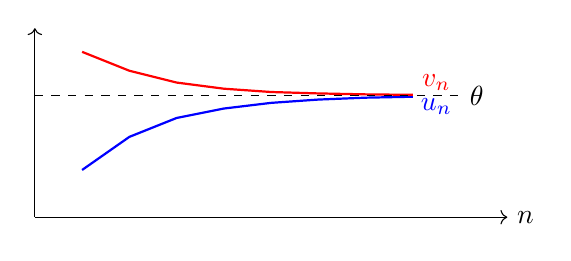
\begin{tikzpicture}[scale=0.6]
\draw[->](0,0)--(10,0) node[right]{$n$};
\draw[->](0,0)--(0,4);
\draw[thick,blue](1,1)--(2,1.7)--(3,2.1)--(4,2.3)--(5,2.42)--(6,2.49)--(7,2.53)--(8,2.55);
\draw[thick,red](1,3.5)--(2,3.1)--(3,2.85)--(4,2.72)--(5,2.65)--(6,2.62)--(7,2.60)--(8,2.59);
\draw[dashed](0,2.57)--(9,2.57) node[right]{$\theta$};
\node[blue]at(8.5,2.35){$u_n$};\node[red]at(8.5,2.85){$v_n$};
\end{tikzpicture}
\caption{Schematic strict bracketing by \(\FormulaFit[\textstyle]{u_n=q_n^{3^{-n}}}\) and \(\FormulaFit[\textstyle]{v_n=(q_n+1)^{3^{-n}}}\). The finite drawn endpoints do not attain the limit.}
\label{fig:mills-recurrence3}
\end{figure}
\begin{figure}[H]\centering
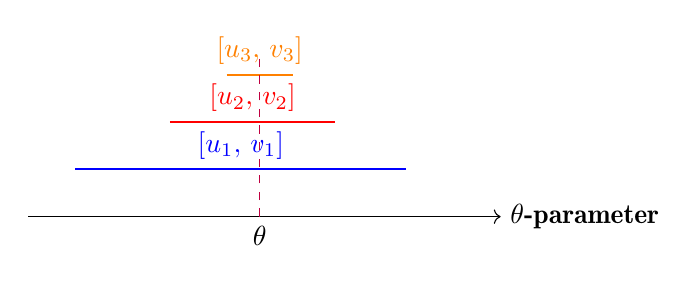
\begin{tikzpicture}[scale=0.6]
\draw[->](0,0)--(10,0) node[right]{$\theta$-parameter};
\draw[thick,blue](1,1)--(8,1) node[midway,above]{$[u_1\comma v_1]$};
\draw[thick,red](3,2)--(6.5,2) node[midway,above]{$[u_2\comma v_2]$};
\draw[thick,orange](4.2,3)--(5.6,3) node[midway,above]{$[u_3\comma v_3]$};
\draw[dashed,purple](4.9,0)--(4.9,3.5);
\node[below]at(4.9,0){$\theta$};
\end{tikzpicture}
\caption{Nested root-transformed intervals \(\FormulaFit[\textstyle]{[q_n^{3^{-n}}\comma (q_n+1)^{3^{-n}}]}\).
The prime-search intervals \(\FormulaFit[\textstyle]{(q_n^3\comma (q_n+1)^3-1)}\) are not nested on the prime scale.}
\label{fig:mills}
\end{figure}
\begin{figure}[H]
	\centering
	\includegraphics[width=0.5\linewidth]{figures/admissible_primes.png}
	\caption{Bounded congruence filtering for parent \(\FormulaFit[\textstyle]{5}\) and four selected
		finite paths with prime values congruent to \(\FormulaFit[\textstyle]{1\pmod4}\).
		The displayed paths do not certify tree extensions to arbitrarily
		large finite heights.}
	\label{fig:mod-primes}
\end{figure}
\begin{figure}[H]
	\centering
	\includegraphics[width=0.4\linewidth]{figures/nested_parameter_cells.png}
	\caption{Three modular inner cells with exact rational endpoints,
		shown on independent axis scales. Decimal labels are approximate;
		exact endpoint numerators are supplied in the \protect\hyperlink{abbr:JSON}{JSON} and \protect\hyperlink{abbr:CSV}{CSV} files.
		These cells certify finite prime-floor conditions, not enclosures
		of a specified global constant.}
	\label{fig:mod-cells}
\end{figure}

\newpage
\begin{thebibliography}{99}
	
	\bibitem{Mills1947}
	\hypertarget{abbr-source:Mills1947}{}
	W.~H.~Mills.
	A prime-representing function.
	\hyperlink{abbr:journal-Bull-Amer-Math-Soc}{\emph{Bull. Amer. Math. Soc.}} \textbf{53} (1947), 604.
	\url{https://doi.org/10.1090/S0002-9904-1947-08849-2}
	
	\bibitem{Kuipers1950}
	\hypertarget{abbr-source:Kuipers1950}{}
	L.~Kuipers.
	Prime-representing functions.
	\hyperlink{abbr:journal-Indag-Math}{\emph{Indag. Math.}} \textbf{12} (1950), 57--58.
	\url{https://zbmath.org/?q=an:0036.05102}
	
	\bibitem{Ansari1951}
	A.~R.~Ansari.
	On prime representing function.
	\emph{Ganita} \textbf{2} (1951), 81--82.
	\url{https://zbmath.org/?q=an:0043.04302}
	
	\bibitem{Wright1951}
	\hypertarget{abbr-source:Wright1951}{}
	E.~M.~Wright.
	A prime-representing function.
	\hyperlink{abbr:journal-Amer-Math-Monthly}{\emph{Amer. Math. Monthly}} \textbf{58} (1951), 616--618.
	\url{https://doi.org/10.2307/2306356}
	
	\bibitem{Ore1952}
	\hypertarget{abbr-source:Ore1952}{}
	O.~Ore.
	On the selection of subsequences.
	\hyperlink{abbr:journal-Proc-Amer-Math-Soc}{\emph{Proc. Amer. Math. Soc.}} \textbf{3} (1952), 706--712.
	\url{https://doi.org/10.1090/S0002-9939-1952-0049977-7}
	
	\bibitem{Niven1951}
	I.~Niven.
	Functions which represent prime numbers.
	\hyperlink{abbr:journal-Proc-Amer-Math-Soc}{\emph{Proc. Amer. Math. Soc.}} \textbf{2} (1951), 753--755.
	\url{https://doi.org/10.1090/S0002-9939-1951-0043804-9}
	
	\bibitem{Wright1954}
	\hypertarget{abbr-source:Wright1954}{}
	E.~M.~Wright.
	A class of representing functions.
	\hyperlink{abbr:journal-J-London-Math-Soc}{\emph{J. London Math. Soc.}} \textbf{29} (1954), 63--71.
	\url{https://doi.org/10.1112/jlms/s1-29.1.63}
	
	\bibitem{Ingham1937}
	\hypertarget{abbr-source:Ingham1937}{}
	A.~E.~Ingham.
	On the difference between consecutive primes.
	\hyperlink{abbr:journal-Quart-J-Math-Oxford-Ser}{\emph{Quart. J. Math. Oxford Ser.}} \textbf{8} (1937), 255--266.
	\url{https://doi.org/10.1093/qmath/os-8.1.255}
	
	\bibitem{Dudley1969}
	U.~Dudley.
	History of a formula for primes.
	\hyperlink{abbr:journal-Amer-Math-Monthly}{\emph{Amer. Math. Monthly}} \textbf{76} (1969), no.~1, 23--28.
	\url{https://doi.org/10.1080/00029890.1969.12000121}
	
	\bibitem{HardyWright1960}
	G.~H.~Hardy and E.~M.~Wright.
	\emph{An Introduction to the Theory of Numbers}, 4th ed.
	Oxford University Press, 1960. Theorem~418.
	\url{https://search.worldcat.org/search?q=An+Introduction+to+the+Theory+of+Numbers+Hardy+Wright}
	
	\bibitem{Simpson2009}
	S.~G.~Simpson.
	\emph{Subsystems of Second Order Arithmetic}, 2nd ed.
	Cambridge University Press, 2009.
	\url{https://doi.org/10.1017/CBO9780511581007}
	
	\bibitem{FormalConjectures}
	Google DeepMind.
	\emph{formal-conjectures}.
	Lean repository, 2026.
	\url{https://github.com/google-deepmind/formal-conjectures}
	\bibitem{MathlibGraph}
	\hypertarget{abbr-source:MathlibGraph}{} X.~Li and P.~Shafto. The Multinetwork of
Mathlib.\newline \hyperlink{abbr:NeurIPS}{NeurIPS} 2026 Datasets and Benchmarks Track (under review).\newline
Dataset files used for the dependency depth:\newline \texttt{v2/declaration/metrics.csv}
(column \texttt{dag\_layer} = topological depth of each declaration in the
declaration \hyperlink{abbr:DAG}{DAG}) and \texttt{mathlib\_edges.csv} (raw dependency edges).\newline
{\scriptsize
	\url{https://huggingface.co/datasets/MathNetwork/MathlibGraph}.\newline
	\url{https://huggingface.co/datasets/MathNetwork/MathlibGraph/resolve/main/v2/declaration/metrics.csv}\newline
	\url{https://huggingface.co/datasets/MathNetwork/MathlibGraph/resolve/main/mathlib_edges.csv}.}

	\bibitem{Bang1952}
	\hypertarget{abbr-source:Bang1952}{}
	T.~Bang.
	A function representing all prime numbers.
	\hyperlink{abbr:journal-Nordisk-Mat-Tidskr}{\emph{Nordisk Mat. Tidskr.}} \textbf{34} (1952), 117--118.
	\url{https://zbmath.org/?q=an:0048.03108}
	
	\bibitem{CaldwellCheng2005}
	\hypertarget{abbr-source:CaldwellCheng2005}{}
	C.~K.~Caldwell and Y.~Cheng.
	Determining Mills' constant and a note on Honaker's problem.
	\hyperlink{abbr:journal-J-Integer-Seq}{\emph{J. Integer Seq.}} \textbf{8} (2005), Article~05.4.1.
	\url{https://cs.uwaterloo.ca/journals/JIS/VOL8/Caldwell/caldwell78.pdf}
	
	\bibitem{Haneke1962}
	\hypertarget{abbr-source:Haneke1962}{}
	W.~Haneke.
	Versch\"arfung der Absch\"atzung von \(\zeta(1/2+it)\).
	\hyperlink{abbr:journal-Acta-Arith}{\emph{Acta Arith.}} \textbf{8} (1962/1963), 357--430.
	\url{https://doi.org/10.4064/aa-8-4-357-430}
	
	\bibitem{Saito2025}
	K.~Saito.
	Mills' constant is irrational.
	\emph{Mathematika} \textbf{71} (2025), no.~3, e70027.
	\url{https://arxiv.org/abs/2404.19461}
	
	\bibitem{Sierpinski1952}
	\hypertarget{abbr-source:Sierpinski1952}{}
	W.~Sierpi\'nski.
	Sur une formule donnant tous les nombres premiers.
	\hyperlink{abbr:journal-C-R-Acad-Sci-Paris}{\emph{C. R. Acad. Sci. Paris}} \textbf{235} (1952), 1078--1079.
	\url{https://gallica.bnf.fr/ark:/12148/bpt6k31936/f1078}
	
	\bibitem{Srinivasan1961}
	\hypertarget{abbr-source:Srinivasan1961}{}
	B.~R.~Srinivasan.
	Formulae for the \(n\)th prime.
	\hyperlink{abbr:journal-J-Indian-Math-Soc}{\emph{J. Indian Math. Soc.}} (\hyperlink{abbr:N.S.}{N.S.}) \textbf{25} (1961), 33--39;
	\textbf{26} (1962), 248.
	\url{https://zbmath.org/?q=an:0111.25002}
	
	\bibitem{Srinivasan1962}
	\hypertarget{abbr-source:Srinivasan1962}{}
	B.~R.~Srinivasan.
	An arithmetical function and an associated formula for the \(n\)th prime,
	I, II.
	\hyperlink{abbr:journal-Norske-Vid-Selsk-Forh-Trondheim}{\emph{Norske Vid. Selsk. Forh. Trondheim}}
	\textbf{35} (1962), 68--71, 72--75.
	\url{https://zbmath.org/?q=an:0117.03003}
	
	\bibitem{Willans1964}
	\hypertarget{abbr-source:Willans1964}{}
	C.~P.~Willans.
	On formulae for the \(n\)th prime number.
	\hyperlink{abbr:journal-Math-Gaz}{\emph{Math. Gaz.}} \textbf{48} (1964), 413--415.
	\url{https://doi.org/10.2307/3611701}
	
	\bibitem{Zach2023}
	R.~Zach.
	Hilbert's Program.
	\emph{Stanford Encyclopedia of Philosophy},
	substantive revision 2023.
	\url{https://plato.stanford.edu/entries/hilbert-program/}
	
	\bibitem{Tait1981}
	\hypertarget{abbr-source:Tait1981}{}
	W.~W.~Tait.
	Finitism.
	\hyperlink{abbr:journal-J-Philosophy}{\emph{J. Philosophy}} \textbf{78} (1981), no.~9, 524--546.
	\url{https://doi.org/10.2307/2026089}
	
	\bibitem{Tait2012}
	\hypertarget{abbr-source:Tait2012}{}
	W.~W.~Tait.
	Primitive Recursive Arithmetic and Its Role in the Foundations of
	Arithmetic: Historical and Philosophical Reflections.
	In \emph{Epistemology versus Ontology},
	\hyperlink{abbr:LEUS}{LEUS} \textbf{27} (2012), 161--180.
	\url{https://doi.org/10.1007/978-94-007-4435-6_8}
	
	\bibitem{Leivant2021}
	\hypertarget{abbr-source:Leivant2021}{}
	D.~Leivant.
	Finitism, imperative programs and primitive recursion.
	\hyperlink{abbr:journal-J-Logic-Comput}{\emph{J. Logic Comput.}} (2021).
	\url{https://doi.org/10.1093/logcom/exaa076}
	
	\bibitem{AvigadGerhardyTowsner2010}
	\hypertarget{abbr-source:AvigadGerhardyTowsner2010}{}
	J.~Avigad, P.~Gerhardy and H.~Towsner.
	Local stability of ergodic averages.
	\hyperlink{abbr:journal-Trans-Amer-Math-Soc}{\emph{Trans. Amer. Math. Soc.}} \textbf{362} (2010), 261--288.
	\url{https://doi.org/10.1090/S0002-9947-09-04814-4}
	
	\bibitem{OConnor2008}
	\hypertarget{abbr-source:OConnor2008}{}
	R.~O'Connor.
	Certified Exact Transcendental Real Number Computation in Coq.
	\emph{\hyperlink{abbr:TPHOLs}{TPHOLs} 2008}, \hyperlink{abbr:LNCS}{LNCS} \textbf{5170}, 246--261.
	\url{https://doi.org/10.1007/978-3-540-71067-7_21}
	
	\bibitem{Elsholtz2020}
	C.~Elsholtz.
	Unconditional Prime-representing Functions, Following Mills.
	\hyperlink{abbr:journal-Amer-Math-Monthly}{\emph{Amer. Math. Monthly}} \textbf{127} (2020), no.~7, 639--642.
	\url{https://doi.org/10.1080/00029890.2020.1751560}
	
	\bibitem{CullyHugill2023}
	\hypertarget{abbr-source:CullyHugill2023}{}
	M.~Cully-Hugill.
	Primes between consecutive powers.
	\hyperlink{abbr:journal-J-Number-Theory}{\emph{J. Number Theory}} \textbf{247} (2023), 100--117.
	\url{https://doi.org/10.1016/j.jnt.2022.12.002}
	
	\bibitem{CullyHugillJohnston2026}
	M.~Cully-Hugill and D.~R.~Johnston.
	On the error term in the explicit formula of Riemann--von Mangoldt II.
	arXiv:2402.04272v3, 23 February 2026; Theorem~1.4.
	\url{https://arxiv.org/abs/2402.04272v3}
	
	\bibitem{Pratt1975}
	\hypertarget{abbr-source:Pratt1975}{}
	V.~R.~Pratt.
	Every Prime Has a Succinct Certificate.
	\hyperlink{abbr:journal-SIAM-J-Comput}{\emph{SIAM J. Comput.}} \textbf{4} (1975), no.~3, 214--220.
	\url{https://doi.org/10.1137/0204018}
	
	\bibitem{MathlibLucas}
	Mathlib contributors.
	The Lucas test for primes.
	Official generated documentation, accessed 20 November 2026.
	\url{https://leanprover-community.github.io/mathlib4_docs/Mathlib/NumberTheory/LucasPrimality.html}
	
	\bibitem{LeanAxioms}
	Lean contributors.
	Axioms.
	\emph{The Lean Language Reference}, chapter~8,
	accessed 20 November 2026.
	\url{https://lean-lang.org/doc/reference/latest/Axioms/}
	
	\bibitem{ThornerZaman2024}
	\hypertarget{abbr-source:ThornerZaman2024}{}
	J.~Thorner and A.~Zaman.
	Refinements to the prime number theorem for arithmetic progressions.
	\hyperlink{abbr:journal-Math-Z}{\emph{Math. Z.}} \textbf{306} (2024), no.~3, Paper~54.
	\url{https://doi.org/10.1007/s00209-023-03414-3}
	Inspected preprint v2, Remark~1.2 and Section~1.2:
	\url{https://arxiv.org/abs/2108.10878v2}.
	
	\bibitem{BennettMartinOBryantRechnitzer2018}
	\hypertarget{abbr-source:BennettMartinOBryantRechnitzer2018}{}
	M.~A.~Bennett, G.~Martin, K.~O'Bryant and A.~Rechnitzer.
	Explicit bounds for primes in arithmetic progressions.
	\hyperlink{abbr:journal-Illinois-J-Math}{\emph{Illinois J. Math.}} \textbf{62} (2018),
	nos.~1--4, 427--532.
	\url{https://arxiv.org/abs/1802.00085v3}
	
	\bibitem{MatomakiMerikoskiTeravainen2024}
	K.~Matom\"aki, J.~Merikoski and J.~Ter\"av\"ainen.
	Primes in arithmetic progressions and short intervals without L-functions.
	Inspected preprint arXiv:2401.17570v1 (2024).
	\url{https://arxiv.org/abs/2401.17570v1}
	

	\bibitem{RealNumbersHistory2005}
	J.~J.~O'Connor and E.~F.~Robertson.
	The real numbers: Stevin to Hilbert.
	\emph{MacTutor History of Mathematics Archive}, October 2005.
	\url{https://mathshistory.st-andrews.ac.uk/HistTopics/Real_numbers_2/}

	\bibitem{Liouville1851}
	J.~Liouville.
	Sur des classes tr\`es-\'etendues de quantit\'es dont la valeur n'est ni
	alg\'ebrique, ni m\^eme r\'eductible \`a des irrationnelles alg\'ebriques.
	\emph{Journal de Math\'ematiques Pures et Appliqu\'ees},
	series~1, \textbf{16} (1851), 133--142.
	\url{https://numdam.org/item/JMPA_1851_1_16__133_0/}

	\bibitem{Turing1936}
	A.~M.~Turing.
	On computable numbers, with an application to the Entscheidungsproblem.
	\emph{Proceedings of the London Mathematical Society},
	series~2, \textbf{42} (1936--1937), 230--265.
	\url{https://doi.org/10.1112/plms/s2-42.1.230}

	\bibitem{TuringCorrection1938}
	A.~M.~Turing.
	On computable numbers, with an application to the Entscheidungsproblem.
	A correction.
	\emph{Proceedings of the London Mathematical Society},
	series~2, \textbf{43} (1938), 544--546.
	\url{https://doi.org/10.1112/plms/s2-43.6.544}
	Open scan: \url{https://www.alice.id.tue.nl/references/turing-1938.pdf}.

	\bibitem{Specker1949}
	E.~Specker.
	Nicht konstruktiv beweisbare S\"atze der Analysis.
	\emph{Journal of Symbolic Logic} \textbf{14} (1949), no.~3, 145--158.
	\url{https://doi.org/10.2307/2267043}

	\bibitem{ConstructiveSEP2022}
	D.~Bridges, E.~Palmgren and H.~Ishihara.
	Constructive Mathematics.
	\emph{Stanford Encyclopedia of Philosophy},
	substantive revision 25 August 2022.
	\url{https://plato.stanford.edu/entries/mathematics-constructive/}

	\bibitem{Bauer2017}
	A.~Bauer.
	Five stages of accepting constructive mathematics.
	\emph{Bulletin of the American Mathematical Society (New Series)}
	\textbf{54} (2017), no.~3, 481--498.
	\url{https://doi.org/10.1090/bull/1556}

	\bibitem{Saito2026}
	K.~Saito.
	Transcendency of variants of Mills' constant.
	\emph{The Ramanujan Journal} \textbf{70} (2026), Article~69.
	Published 10 August 2026.
	\url{https://doi.org/10.1007/s11139-026-01443-0}
	Open preprint: arXiv:2508.16068v3, 7 December 2025,
	Theorems~1.7--1.8.
	\url{https://arxiv.org/abs/2508.16068v3}

	\bibitem{KaratarakisWiedijk2026}
	M.~Karatarakis and F.~Wiedijk.
	A formalization of the Gelfond-Schneider theorem.
	Preprint, arXiv:2603.24823v1, 25 March 2026;
	Theorem~3.1 and Lemma~7.
	\url{https://arxiv.org/abs/2603.24823v1}

	\bibitem{LeanDefinitions}
	Lean contributors.
	Modifiers; Recursive Definitions.
	\emph{The Lean Language Reference}, Sections~7.1 and~7.6.2.4,
	accessed 20 November 2026.
	\url{https://lean-lang.org/doc/reference/latest/Definitions/Modifiers/}
	\url{https://lean-lang.org/doc/reference/latest/Definitions/Recursive-Definitions/}

\end{thebibliography}

\end{document}
